\documentclass[a4paper]{book}
\usepackage{makeidx}
\usepackage{natbib}
\usepackage{graphicx}
\usepackage{multicol}
\usepackage{float}
\usepackage{listings}
\usepackage{color}
\usepackage{ifthen}
\usepackage[table]{xcolor}
\usepackage{textcomp}
\usepackage{alltt}
\usepackage{ifpdf}
\ifpdf
\usepackage[pdftex,
            pagebackref=true,
            colorlinks=true,
            linkcolor=blue,
            unicode
           ]{hyperref}
\else
\usepackage[ps2pdf,
            pagebackref=true,
            colorlinks=true,
            linkcolor=blue,
            unicode
           ]{hyperref}
\usepackage{pspicture}
\fi
\usepackage[utf8]{inputenc}
\usepackage{mathptmx}
\usepackage[scaled=.90]{helvet}
\usepackage{courier}
\usepackage{sectsty}
\usepackage[titles]{tocloft}
\usepackage{doxygen}
\lstset{language=C++,inputencoding=utf8,basicstyle=\footnotesize,breaklines=true,breakatwhitespace=true,tabsize=4,numbers=left }
\usepackage{amsmath}
\usepackage{amsfonts}
\usepackage{mathtools}
\makeindex
\setcounter{tocdepth}{3}
\renewcommand{\footrulewidth}{0.4pt}
\renewcommand{\familydefault}{\sfdefault}
\hfuzz=15pt
\setlength{\emergencystretch}{15pt}
\hbadness=750
\tolerance=750
\begin{document}
\hypersetup{pageanchor=false,citecolor=blue}
\begin{titlepage}
\vspace*{7cm}
\begin{center}
{\Large ocra-\/wbi-\/plugins }\\
\vspace*{1cm}
{\large \-Generated by Doxygen 1.7.6.1}\\
\vspace*{0.5cm}
{\small Fri Dec 16 2016 17:50:12}\\
\end{center}
\end{titlepage}
\clearemptydoublepage
\pagenumbering{roman}
\tableofcontents
\clearemptydoublepage
\pagenumbering{arabic}
\hypersetup{pageanchor=true,citecolor=blue}
\chapter{\-Todo \-List}
\label{todo}
\hypertarget{todo}{}

\begin{DoxyRefList}
\item[\label{todo__todo000002}%
\hypertarget{todo__todo000002}{}%
\-Member \hyperlink{classSteppingDemoClient_ad8fbc186267a47a73bb77e78199f2b8c}{\-Stepping\-Demo\-Client\-:\-:is\-Balanced} ()]\-A more balance-\/centered criterion should be used for this, \-Z\-M\-P-\/based for example.  
\item[\label{todo__todo000001}%
\hypertarget{todo__todo000001}{}%
\-Class \hyperlink{classThread}{\-Thread} ]\-Remove task sequences. \-This class sets up an ocra\-::\-Model which is constructed from an \-Ocra\-Wbi\-Model and an ocra\-::\-Controller which can be specified as either a \-Wocra\-Controller, a \-Gocra\-Controller, or a \-Hocra\-Controller. \-The thread is looped at the period specified by the user (defaults to 10ms) and on each loop the \-Model is updated and the control torques are recalculated. $\ast$\-At the writing of this comment, task sequences are still in use and they too are initialized and updated here. \-They will be removed eventually.$\ast$ 
\end{DoxyRefList}
\chapter{\-Namespace \-Index}
\section{\-Namespace \-List}
\-Here is a list of all namespaces with brief descriptions\-:\begin{DoxyCompactList}
\item\contentsline{section}{\hyperlink{namespaceocra__icub}{ocra\-\_\-icub} }{\pageref{namespaceocra__icub}}{}
\end{DoxyCompactList}

\chapter{\-Class \-Index}
\section{\-Class \-List}
\-Here are the classes, structs, unions and interfaces with brief descriptions\-:\begin{DoxyCompactList}
\item\contentsline{section}{\hyperlink{classAdmissibilityConstraints}{\-Admissibility\-Constraints} }{\pageref{classAdmissibilityConstraints}}{}
\item\contentsline{section}{\hyperlink{structAdmissibilityConstraintsStruct}{\-Admissibility\-Constraints\-Struct} }{\pageref{structAdmissibilityConstraintsStruct}}{}
\item\contentsline{section}{\hyperlink{classBaseOfSupport}{\-Base\-Of\-Support} \\*\-Builds base of support and corresponding constraints based on the robot's feet location }{\pageref{classBaseOfSupport}}{}
\item\contentsline{section}{\hyperlink{classBounding}{\-Bounding} }{\pageref{classBounding}}{}
\item\contentsline{section}{\hyperlink{structShapeConstraintsStruct_1_1boundingStruct}{\-Shape\-Constraints\-Struct\-::bounding\-Struct} }{\pageref{structShapeConstraintsStruct_1_1boundingStruct}}{}
\item\contentsline{section}{\hyperlink{classConstancy}{\-Constancy} }{\pageref{classConstancy}}{}
\item\contentsline{section}{\hyperlink{structShapeConstraintsStruct_1_1constancyStruct}{\-Shape\-Constraints\-Struct\-::constancy\-Struct} }{\pageref{structShapeConstraintsStruct_1_1constancyStruct}}{}
\item\contentsline{section}{\hyperlink{classConstraint}{\-Constraint} }{\pageref{classConstraint}}{}
\item\contentsline{section}{\hyperlink{classContactConfigEnforcement}{\-Contact\-Config\-Enforcement} }{\pageref{classContactConfigEnforcement}}{}
\item\contentsline{section}{\hyperlink{classContactConfigHistory}{\-Contact\-Config\-History} }{\pageref{classContactConfigHistory}}{}
\item\contentsline{section}{\hyperlink{structAdmissibilityConstraintsStruct_1_1ContactConfigurationEnforcement}{\-Admissibility\-Constraints\-Struct\-::\-Contact\-Configuration\-Enforcement} }{\pageref{structAdmissibilityConstraintsStruct_1_1ContactConfigurationEnforcement}}{}
\item\contentsline{section}{\hyperlink{structAdmissibilityConstraintsStruct_1_1ContactConfigurationHistory}{\-Admissibility\-Constraints\-Struct\-::\-Contact\-Configuration\-History} }{\pageref{structAdmissibilityConstraintsStruct_1_1ContactConfigurationHistory}}{}
\item\contentsline{section}{\hyperlink{classThread_1_1ControllerRpcServerCallback}{\-Thread\-::\-Controller\-Rpc\-Server\-Callback} \\*\-A callback function which binds the rpc server port opened in the contoller server module to the controller thread's parsing function }{\pageref{classThread_1_1ControllerRpcServerCallback}}{}
\item\contentsline{section}{\hyperlink{classThread_1_1DebugRpcServerCallback}{\-Thread\-::\-Debug\-Rpc\-Server\-Callback} \\*\-A callback function which binds the rpc server port opened in the contoller server module to the controller thread's parsing function }{\pageref{classThread_1_1DebugRpcServerCallback}}{}
\item\contentsline{section}{\hyperlink{classExampleClient}{\-Example\-Client} }{\pageref{classExampleClient}}{}
\item\contentsline{section}{\hyperlink{classIcubControllerServer}{\-Icub\-Controller\-Server} }{\pageref{classIcubControllerServer}}{}
\item\contentsline{section}{\hyperlink{classMIQPController}{\-M\-I\-Q\-P\-Controller} }{\pageref{classMIQPController}}{}
\item\contentsline{section}{\hyperlink{classMIQPLinearConstraints}{\-M\-I\-Q\-P\-Linear\-Constraints} }{\pageref{classMIQPLinearConstraints}}{}
\item\contentsline{section}{\hyperlink{structMIQPParameters}{\-M\-I\-Q\-P\-Parameters} }{\pageref{structMIQPParameters}}{}
\item\contentsline{section}{\hyperlink{classMIQP_1_1MIQPState}{\-M\-I\-Q\-P\-::\-M\-I\-Q\-P\-State} }{\pageref{classMIQP_1_1MIQPState}}{}
\item\contentsline{section}{\hyperlink{classMIQPState}{\-M\-I\-Q\-P\-State} \\*\-Takes care of updating the state defined for the \hyperlink{namespaceMIQP}{\-M\-I\-Q\-P} problem }{\pageref{classMIQPState}}{}
\item\contentsline{section}{\hyperlink{classocra__icub_1_1ModelInitializer}{ocra\-\_\-icub\-::\-Model\-Initializer} }{\pageref{classocra__icub_1_1ModelInitializer}}{}
\item\contentsline{section}{\hyperlink{classModule}{\-Module} \\*\-The controller module which launches the controller thread }{\pageref{classModule}}{}
\item\contentsline{section}{\hyperlink{classOcraControllerOptions}{\-Ocra\-Controller\-Options} }{\pageref{classOcraControllerOptions}}{}
\item\contentsline{section}{\hyperlink{classocra__icub_1_1OcraWbiConversions}{ocra\-\_\-icub\-::\-Ocra\-Wbi\-Conversions} }{\pageref{classocra__icub_1_1OcraWbiConversions}}{}
\item\contentsline{section}{\hyperlink{classocra__icub_1_1OcraWbiModel}{ocra\-\_\-icub\-::\-Ocra\-Wbi\-Model} }{\pageref{classocra__icub_1_1OcraWbiModel}}{}
\item\contentsline{section}{\hyperlink{structOcraWbiModel_1_1OcraWbiModel__pimpl}{ocra\-\_\-icub\-::\-Ocra\-Wbi\-Model\-::\-Ocra\-Wbi\-Model\-\_\-pimpl} }{\pageref{structOcraWbiModel_1_1OcraWbiModel__pimpl}}{}
\item\contentsline{section}{\hyperlink{classSequentiality}{\-Sequentiality} }{\pageref{classSequentiality}}{}
\item\contentsline{section}{\hyperlink{structShapeConstraintsStruct_1_1sequentialityStruct}{\-Shape\-Constraints\-Struct\-::sequentiality\-Struct} }{\pageref{structShapeConstraintsStruct_1_1sequentialityStruct}}{}
\item\contentsline{section}{\hyperlink{classShapeConstraints}{\-Shape\-Constraints} }{\pageref{classShapeConstraints}}{}
\item\contentsline{section}{\hyperlink{structShapeConstraintsStruct}{\-Shape\-Constraints\-Struct} }{\pageref{structShapeConstraintsStruct}}{}
\item\contentsline{section}{\hyperlink{structsingleStepTestParams}{single\-Step\-Test\-Params} }{\pageref{structsingleStepTestParams}}{}
\item\contentsline{section}{\hyperlink{classSingleSupport}{\-Single\-Support} }{\pageref{classSingleSupport}}{}
\item\contentsline{section}{\hyperlink{structAdmissibilityConstraintsStruct_1_1SingleSupport}{\-Admissibility\-Constraints\-Struct\-::\-Single\-Support} }{\pageref{structAdmissibilityConstraintsStruct_1_1SingleSupport}}{}
\item\contentsline{section}{\hyperlink{classSittingDemoClient}{\-Sitting\-Demo\-Client} }{\pageref{classSittingDemoClient}}{}
\item\contentsline{section}{\hyperlink{structAdmissibilityConstraintsStruct_1_1SSandDSAlternation}{\-Admissibility\-Constraints\-Struct\-::\-S\-Sand\-D\-S\-Alternation} }{\pageref{structAdmissibilityConstraintsStruct_1_1SSandDSAlternation}}{}
\item\contentsline{section}{\hyperlink{classSSDSAlternation}{\-S\-S\-D\-S\-Alternation} }{\pageref{classSSDSAlternation}}{}
\item\contentsline{section}{\hyperlink{classStandingDemoClient}{\-Standing\-Demo\-Client} }{\pageref{classStandingDemoClient}}{}
\item\contentsline{section}{\hyperlink{classStepController}{\-Step\-Controller} }{\pageref{classStepController}}{}
\item\contentsline{section}{\hyperlink{classSteppingDemoClient}{\-Stepping\-Demo\-Client} }{\pageref{classSteppingDemoClient}}{}
\item\contentsline{section}{\hyperlink{structsteppingTestParams}{stepping\-Test\-Params} }{\pageref{structsteppingTestParams}}{}
\item\contentsline{section}{\hyperlink{classTaskOpsClient}{\-Task\-Ops\-Client} }{\pageref{classTaskOpsClient}}{}
\item\contentsline{section}{\hyperlink{classThread}{\-Thread} \\*\-The meat and potatoes of the controller server }{\pageref{classThread}}{}
\item\contentsline{section}{\hyperlink{classWalkingClient}{\-Walking\-Client} }{\pageref{classWalkingClient}}{}
\item\contentsline{section}{\hyperlink{structWalkingParams}{\-Walking\-Params} }{\pageref{structWalkingParams}}{}
\item\contentsline{section}{\hyperlink{classZmpController}{\-Zmp\-Controller} \\*\-Implementes a \-Z\-M\-P controller as a force set point regulator }{\pageref{classZmpController}}{}
\item\contentsline{section}{\hyperlink{structZmpControllerParams}{\-Zmp\-Controller\-Params} }{\pageref{structZmpControllerParams}}{}
\item\contentsline{section}{\hyperlink{classZmpPreviewController}{\-Zmp\-Preview\-Controller} \\*\-Implementes an extended \-Z\-M\-P preview controller as an unconstrained \-Q\-P problem }{\pageref{classZmpPreviewController}}{}
\item\contentsline{section}{\hyperlink{structZmpPreviewParams}{\-Zmp\-Preview\-Params} }{\pageref{structZmpPreviewParams}}{}
\end{DoxyCompactList}

\chapter{\-File \-Index}
\section{\-File \-List}
\-Here is a list of all files with brief descriptions\-:\begin{DoxyCompactList}
\item\contentsline{section}{ocra-\/wbi-\/plugins/\hyperlink{README_8md}{\-R\-E\-A\-D\-M\-E.\-md} }{\pageref{README_8md}}{}
\item\contentsline{section}{ocra-\/wbi-\/plugins/ocra-\/icub-\/clients/example-\/client/include/example-\/client/\hyperlink{ExampleClient_8h}{\-Example\-Client.\-h} }{\pageref{ExampleClient_8h}}{}
\item\contentsline{section}{ocra-\/wbi-\/plugins/ocra-\/icub-\/clients/example-\/client/src/\hyperlink{example-client_8cpp}{example-\/client.\-cpp} }{\pageref{example-client_8cpp}}{}
\item\contentsline{section}{ocra-\/wbi-\/plugins/ocra-\/icub-\/clients/example-\/client/src/\hyperlink{ExampleClient_8cpp}{\-Example\-Client.\-cpp} }{\pageref{ExampleClient_8cpp}}{}
\item\contentsline{section}{ocra-\/wbi-\/plugins/ocra-\/icub-\/clients/sitting-\/demo/include/sitting-\/demo/\hyperlink{SittingDemoClient_8h}{\-Sitting\-Demo\-Client.\-h} }{\pageref{SittingDemoClient_8h}}{}
\item\contentsline{section}{ocra-\/wbi-\/plugins/ocra-\/icub-\/clients/sitting-\/demo/src/\hyperlink{ocra-icub-clients_2sitting-demo_2src_2main_8cpp}{main.\-cpp} }{\pageref{ocra-icub-clients_2sitting-demo_2src_2main_8cpp}}{}
\item\contentsline{section}{ocra-\/wbi-\/plugins/ocra-\/icub-\/clients/sitting-\/demo/src/\hyperlink{SittingDemoClient_8cpp}{\-Sitting\-Demo\-Client.\-cpp} }{\pageref{SittingDemoClient_8cpp}}{}
\item\contentsline{section}{ocra-\/wbi-\/plugins/ocra-\/icub-\/clients/standing-\/demo/include/standing-\/demo/\hyperlink{StandingDemoClient_8h}{\-Standing\-Demo\-Client.\-h} }{\pageref{StandingDemoClient_8h}}{}
\item\contentsline{section}{ocra-\/wbi-\/plugins/ocra-\/icub-\/clients/standing-\/demo/src/\hyperlink{ocra-icub-clients_2standing-demo_2src_2main_8cpp}{main.\-cpp} }{\pageref{ocra-icub-clients_2standing-demo_2src_2main_8cpp}}{}
\item\contentsline{section}{ocra-\/wbi-\/plugins/ocra-\/icub-\/clients/standing-\/demo/src/\hyperlink{StandingDemoClient_8cpp}{\-Standing\-Demo\-Client.\-cpp} }{\pageref{StandingDemoClient_8cpp}}{}
\item\contentsline{section}{ocra-\/wbi-\/plugins/ocra-\/icub-\/clients/stepping-\/demo/include/stepping-\/demo/\hyperlink{SteppingDemoClient_8h}{\-Stepping\-Demo\-Client.\-h} }{\pageref{SteppingDemoClient_8h}}{}
\item\contentsline{section}{ocra-\/wbi-\/plugins/ocra-\/icub-\/clients/stepping-\/demo/src/\hyperlink{stepping-demo_8cpp}{stepping-\/demo.\-cpp} }{\pageref{stepping-demo_8cpp}}{}
\item\contentsline{section}{ocra-\/wbi-\/plugins/ocra-\/icub-\/clients/stepping-\/demo/src/\hyperlink{SteppingDemoClient_8cpp}{\-Stepping\-Demo\-Client.\-cpp} }{\pageref{SteppingDemoClient_8cpp}}{}
\item\contentsline{section}{ocra-\/wbi-\/plugins/ocra-\/icub-\/clients/task-\/operations-\/demo/include/task-\/operations-\/demo/\hyperlink{TaskOpsClient_8h}{\-Task\-Ops\-Client.\-h} }{\pageref{TaskOpsClient_8h}}{}
\item\contentsline{section}{ocra-\/wbi-\/plugins/ocra-\/icub-\/clients/task-\/operations-\/demo/src/\hyperlink{task-operations-demo_8cpp}{task-\/operations-\/demo.\-cpp} }{\pageref{task-operations-demo_8cpp}}{}
\item\contentsline{section}{ocra-\/wbi-\/plugins/ocra-\/icub-\/clients/task-\/operations-\/demo/src/\hyperlink{TaskOpsClient_8cpp}{\-Task\-Ops\-Client.\-cpp} }{\pageref{TaskOpsClient_8cpp}}{}
\item\contentsline{section}{ocra-\/wbi-\/plugins/ocra-\/icub-\/clients/walking-\/client/include/walking-\/client/\hyperlink{WalkingClient_8h}{\-Walking\-Client.\-h} }{\pageref{WalkingClient_8h}}{}
\item\contentsline{section}{ocra-\/wbi-\/plugins/ocra-\/icub-\/clients/walking-\/client/include/walking-\/client/\hyperlink{ZmpController_8h}{\-Zmp\-Controller.\-h} }{\pageref{ZmpController_8h}}{}
\item\contentsline{section}{ocra-\/wbi-\/plugins/ocra-\/icub-\/clients/walking-\/client/include/walking-\/client/\hyperlink{ZmpPreviewController_8h}{\-Zmp\-Preview\-Controller.\-h} }{\pageref{ZmpPreviewController_8h}}{}
\item\contentsline{section}{ocra-\/wbi-\/plugins/ocra-\/icub-\/clients/walking-\/client/src/\hyperlink{ocra-icub-clients_2walking-client_2src_2main_8cpp}{main.\-cpp} }{\pageref{ocra-icub-clients_2walking-client_2src_2main_8cpp}}{}
\item\contentsline{section}{ocra-\/wbi-\/plugins/ocra-\/icub-\/clients/walking-\/client/src/\hyperlink{WalkingClient_8cpp}{\-Walking\-Client.\-cpp} }{\pageref{WalkingClient_8cpp}}{}
\item\contentsline{section}{ocra-\/wbi-\/plugins/ocra-\/icub-\/clients/walking-\/client/src/\hyperlink{ZmpController_8cpp}{\-Zmp\-Controller.\-cpp} }{\pageref{ZmpController_8cpp}}{}
\item\contentsline{section}{ocra-\/wbi-\/plugins/ocra-\/icub-\/clients/walking-\/client/src/\hyperlink{ZmpPreviewController_8cpp}{\-Zmp\-Preview\-Controller.\-cpp} }{\pageref{ZmpPreviewController_8cpp}}{}
\item\contentsline{section}{ocra-\/wbi-\/plugins/ocra-\/icub-\/server/include/ocra-\/icub-\/server/\hyperlink{IcubControllerServer_8h}{\-Icub\-Controller\-Server.\-h} }{\pageref{IcubControllerServer_8h}}{}
\item\contentsline{section}{ocra-\/wbi-\/plugins/ocra-\/icub-\/server/include/ocra-\/icub-\/server/\hyperlink{Module_8h}{\-Module.\-h} \\*\hyperlink{classModule}{\-Module} class for the controller server }{\pageref{Module_8h}}{}
\item\contentsline{section}{ocra-\/wbi-\/plugins/ocra-\/icub-\/server/include/ocra-\/icub-\/server/\hyperlink{Thread_8h}{\-Thread.\-h} \\*\-The thread class for the controller server }{\pageref{Thread_8h}}{}
\item\contentsline{section}{ocra-\/wbi-\/plugins/ocra-\/icub-\/server/src/\hyperlink{IcubControllerServer_8cpp}{\-Icub\-Controller\-Server.\-cpp} }{\pageref{IcubControllerServer_8cpp}}{}
\item\contentsline{section}{ocra-\/wbi-\/plugins/ocra-\/icub-\/server/src/\hyperlink{ocra-icub-server_2src_2main_8cpp}{main.\-cpp} }{\pageref{ocra-icub-server_2src_2main_8cpp}}{}
\item\contentsline{section}{ocra-\/wbi-\/plugins/ocra-\/icub-\/server/src/\hyperlink{Module_8cpp}{\-Module.\-cpp} }{\pageref{Module_8cpp}}{}
\item\contentsline{section}{ocra-\/wbi-\/plugins/ocra-\/icub-\/server/src/\hyperlink{Thread_8cpp}{\-Thread.\-cpp} \\*\-The thread class for the controller server }{\pageref{Thread_8cpp}}{}
\item\contentsline{section}{ocra-\/wbi-\/plugins/ocra-\/icub/include/ocra-\/icub/\hyperlink{IcubClient_8h}{\-Icub\-Client.\-h} }{\pageref{IcubClient_8h}}{}
\item\contentsline{section}{ocra-\/wbi-\/plugins/ocra-\/icub/include/ocra-\/icub/\hyperlink{ModelInitializer_8h}{\-Model\-Initializer.\-h} }{\pageref{ModelInitializer_8h}}{}
\item\contentsline{section}{ocra-\/wbi-\/plugins/ocra-\/icub/include/ocra-\/icub/\hyperlink{OcraWbiConversions_8h}{\-Ocra\-Wbi\-Conversions.\-h} \\*\-A utility class full of static conversion functions }{\pageref{OcraWbiConversions_8h}}{}
\item\contentsline{section}{ocra-\/wbi-\/plugins/ocra-\/icub/include/ocra-\/icub/\hyperlink{OcraWbiModel_8h}{\-Ocra\-Wbi\-Model.\-h} \\*\-Implementation of ocra\-::\-Model using whole\-Body\-Interface }{\pageref{OcraWbiModel_8h}}{}
\item\contentsline{section}{ocra-\/wbi-\/plugins/ocra-\/icub/include/ocra-\/icub/\hyperlink{Utilities_8h}{\-Utilities.\-h} \\*\-Some useful tools for the ocra-\/icub lib }{\pageref{Utilities_8h}}{}
\item\contentsline{section}{ocra-\/wbi-\/plugins/ocra-\/icub/src/\hyperlink{ModelInitializer_8cpp}{\-Model\-Initializer.\-cpp} }{\pageref{ModelInitializer_8cpp}}{}
\item\contentsline{section}{ocra-\/wbi-\/plugins/ocra-\/icub/src/\hyperlink{OcraWbiConversions_8cpp}{\-Ocra\-Wbi\-Conversions.\-cpp} \\*\-A utility class full of static conversion functions }{\pageref{OcraWbiConversions_8cpp}}{}
\item\contentsline{section}{ocra-\/wbi-\/plugins/ocra-\/icub/src/\hyperlink{OcraWbiModel_8cpp}{\-Ocra\-Wbi\-Model.\-cpp} \\*\-Implementation of ocra\-::\-Model using whole\-Body\-Interface }{\pageref{OcraWbiModel_8cpp}}{}
\item\contentsline{section}{ocra-\/wbi-\/plugins/ocra-\/icub/src/\hyperlink{Utilities_8cpp}{\-Utilities.\-cpp} \\*\-Some useful tools for the ocra-\/icub lib }{\pageref{Utilities_8cpp}}{}
\end{DoxyCompactList}

\chapter{\-Namespace \-Documentation}
\hypertarget{namespaceocra__icub}{\section{ocra\-\_\-icub \-Namespace \-Reference}
\label{namespaceocra__icub}\index{ocra\-\_\-icub@{ocra\-\_\-icub}}
}
\subsection*{\-Classes}
\begin{DoxyCompactItemize}
\item 
class \hyperlink{classocra__icub_1_1ModelInitializer}{\-Model\-Initializer}
\item 
class \hyperlink{classocra__icub_1_1OcraWbiConversions}{\-Ocra\-Wbi\-Conversions}
\item 
class \hyperlink{classocra__icub_1_1OcraWbiModel}{\-Ocra\-Wbi\-Model}
\end{DoxyCompactItemize}
\subsection*{\-Typedefs}
\begin{DoxyCompactItemize}
\item 
typedef \-Eigen\-::\-Matrix$<$ double, \*
\-Eigen\-::\-Dynamic, \-Eigen\-::\-Dynamic, \*
\-Eigen\-::\-Row\-Major $>$ \hyperlink{namespaceocra__icub_aa5e36a19ed031c28ca83c207bd7dd83f}{\-Matrix\-Xd\-Rm}
\end{DoxyCompactItemize}
\subsection*{\-Enumerations}
\begin{DoxyCompactItemize}
\item 
enum \hyperlink{namespaceocra__icub_afbd2db66b68005fb7cfac19210caf83f}{\-O\-C\-R\-A\-\_\-\-I\-C\-U\-B\-\_\-\-M\-E\-S\-S\-A\-G\-E} \{ \*
\hyperlink{namespaceocra__icub_afbd2db66b68005fb7cfac19210caf83fafa982af27b4e13f109d8769472d75217}{\-S\-T\-R\-I\-N\-G\-\_\-\-M\-E\-S\-S\-A\-G\-E} =  -\/1, 
\hyperlink{namespaceocra__icub_afbd2db66b68005fb7cfac19210caf83faa0c1832978fad84ef108d48265af68d2}{\-F\-A\-I\-L\-U\-R\-E} =  0, 
\hyperlink{namespaceocra__icub_afbd2db66b68005fb7cfac19210caf83fa67c96e3afcb39533f69c97dc5e9734e5}{\-S\-U\-C\-C\-E\-S\-S}, 
\hyperlink{namespaceocra__icub_afbd2db66b68005fb7cfac19210caf83fae8fe02f5f3b1b11d4749e720b9ec3636}{\-G\-E\-T\-\_\-\-M\-O\-D\-E\-L\-\_\-\-C\-O\-N\-F\-I\-G\-\_\-\-I\-N\-F\-O}, 
\*
\hyperlink{namespaceocra__icub_afbd2db66b68005fb7cfac19210caf83fa772ab917d1ff28db029af9271208a69a}{\-G\-E\-T\-\_\-\-C\-O\-N\-T\-R\-O\-L\-L\-E\-R\-\_\-\-S\-E\-R\-V\-E\-R\-\_\-\-S\-T\-A\-T\-U\-S}, 
\hyperlink{namespaceocra__icub_afbd2db66b68005fb7cfac19210caf83fa5dee3cfa0ab6c29f5546bc9e30c0aef5}{\-C\-O\-N\-T\-R\-O\-L\-L\-E\-R\-\_\-\-S\-E\-R\-V\-E\-R\-\_\-\-R\-U\-N\-N\-I\-N\-G}, 
\hyperlink{namespaceocra__icub_afbd2db66b68005fb7cfac19210caf83fafd31e40d18e553fc09105d360455bc49}{\-C\-O\-N\-T\-R\-O\-L\-L\-E\-R\-\_\-\-S\-E\-R\-V\-E\-R\-\_\-\-S\-T\-O\-P\-P\-E\-D}, 
\hyperlink{namespaceocra__icub_afbd2db66b68005fb7cfac19210caf83fa48ad7962d035a58257a0381872ce27b1}{\-C\-O\-N\-T\-R\-O\-L\-L\-E\-R\-\_\-\-S\-E\-R\-V\-E\-R\-\_\-\-P\-A\-U\-S\-E\-D}, 
\*
\hyperlink{namespaceocra__icub_afbd2db66b68005fb7cfac19210caf83fafd78d107914396f475c3b12d2b31ea2a}{\-G\-E\-T\-\_\-\-L\-\_\-\-F\-O\-O\-T\-\_\-\-P\-O\-S\-E}, 
\hyperlink{namespaceocra__icub_afbd2db66b68005fb7cfac19210caf83fae7c9fa2563b6c0b14e5b05d1794dac36}{\-H\-E\-L\-P}
 \}
\end{DoxyCompactItemize}
\subsection*{\-Functions}
\begin{DoxyCompactItemize}
\item 
void \hyperlink{namespaceocra__icub_a07ffe33877389b6b111944e8a666e221}{get\-Nominal\-Posture} (const ocra\-::\-Model \&model, \-Eigen\-::\-Vector\-Xd \&q)
\item 
void \hyperlink{namespaceocra__icub_a91c3caf94014ea9988e56dd2572768ce}{get\-Home\-Posture} (const ocra\-::\-Model \&model, \-Eigen\-::\-Vector\-Xd \&q)
\end{DoxyCompactItemize}
\subsection*{\-Variables}
\begin{DoxyCompactItemize}
\item 
static constexpr double \hyperlink{namespaceocra__icub_ab06477ded34ed5514b911a3511b22e3d}{\-D\-E\-G\-\_\-\-T\-O\-\_\-\-R\-A\-D} = \-M\-\_\-\-P\-I/180.\-0
\end{DoxyCompactItemize}


\subsection{\-Typedef \-Documentation}
\hypertarget{namespaceocra__icub_aa5e36a19ed031c28ca83c207bd7dd83f}{\index{ocra\-\_\-icub@{ocra\-\_\-icub}!\-Matrix\-Xd\-Rm@{\-Matrix\-Xd\-Rm}}
\index{\-Matrix\-Xd\-Rm@{\-Matrix\-Xd\-Rm}!ocra_icub@{ocra\-\_\-icub}}
\subsubsection[{\-Matrix\-Xd\-Rm}]{\setlength{\rightskip}{0pt plus 5cm}typedef \-Eigen\-::\-Matrix$<$double, \-Eigen\-::\-Dynamic, \-Eigen\-::\-Dynamic, \-Eigen\-::\-Row\-Major$>$ {\bf ocra\-\_\-icub\-::\-Matrix\-Xd\-Rm}}}\label{namespaceocra__icub_aa5e36a19ed031c28ca83c207bd7dd83f}


\subsection{\-Enumeration \-Type \-Documentation}
\hypertarget{namespaceocra__icub_afbd2db66b68005fb7cfac19210caf83f}{\index{ocra\-\_\-icub@{ocra\-\_\-icub}!\-O\-C\-R\-A\-\_\-\-I\-C\-U\-B\-\_\-\-M\-E\-S\-S\-A\-G\-E@{\-O\-C\-R\-A\-\_\-\-I\-C\-U\-B\-\_\-\-M\-E\-S\-S\-A\-G\-E}}
\index{\-O\-C\-R\-A\-\_\-\-I\-C\-U\-B\-\_\-\-M\-E\-S\-S\-A\-G\-E@{\-O\-C\-R\-A\-\_\-\-I\-C\-U\-B\-\_\-\-M\-E\-S\-S\-A\-G\-E}!ocra_icub@{ocra\-\_\-icub}}
\subsubsection[{\-O\-C\-R\-A\-\_\-\-I\-C\-U\-B\-\_\-\-M\-E\-S\-S\-A\-G\-E}]{\setlength{\rightskip}{0pt plus 5cm}enum {\bf ocra\-\_\-icub\-::\-O\-C\-R\-A\-\_\-\-I\-C\-U\-B\-\_\-\-M\-E\-S\-S\-A\-G\-E}}}\label{namespaceocra__icub_afbd2db66b68005fb7cfac19210caf83f}
\begin{Desc}
\item[\-Enumerator\-: ]\par
\begin{description}
\index{\-S\-T\-R\-I\-N\-G\-\_\-\-M\-E\-S\-S\-A\-G\-E@{\-S\-T\-R\-I\-N\-G\-\_\-\-M\-E\-S\-S\-A\-G\-E}!ocra\-\_\-icub@{ocra\-\_\-icub}}\index{ocra\-\_\-icub@{ocra\-\_\-icub}!\-S\-T\-R\-I\-N\-G\-\_\-\-M\-E\-S\-S\-A\-G\-E@{\-S\-T\-R\-I\-N\-G\-\_\-\-M\-E\-S\-S\-A\-G\-E}}\item[{\em 
\hypertarget{namespaceocra__icub_afbd2db66b68005fb7cfac19210caf83fafa982af27b4e13f109d8769472d75217}{\-S\-T\-R\-I\-N\-G\-\_\-\-M\-E\-S\-S\-A\-G\-E}\label{namespaceocra__icub_afbd2db66b68005fb7cfac19210caf83fafa982af27b4e13f109d8769472d75217}
}]\index{\-F\-A\-I\-L\-U\-R\-E@{\-F\-A\-I\-L\-U\-R\-E}!ocra\-\_\-icub@{ocra\-\_\-icub}}\index{ocra\-\_\-icub@{ocra\-\_\-icub}!\-F\-A\-I\-L\-U\-R\-E@{\-F\-A\-I\-L\-U\-R\-E}}\item[{\em 
\hypertarget{namespaceocra__icub_afbd2db66b68005fb7cfac19210caf83faa0c1832978fad84ef108d48265af68d2}{\-F\-A\-I\-L\-U\-R\-E}\label{namespaceocra__icub_afbd2db66b68005fb7cfac19210caf83faa0c1832978fad84ef108d48265af68d2}
}]\index{\-S\-U\-C\-C\-E\-S\-S@{\-S\-U\-C\-C\-E\-S\-S}!ocra\-\_\-icub@{ocra\-\_\-icub}}\index{ocra\-\_\-icub@{ocra\-\_\-icub}!\-S\-U\-C\-C\-E\-S\-S@{\-S\-U\-C\-C\-E\-S\-S}}\item[{\em 
\hypertarget{namespaceocra__icub_afbd2db66b68005fb7cfac19210caf83fa67c96e3afcb39533f69c97dc5e9734e5}{\-S\-U\-C\-C\-E\-S\-S}\label{namespaceocra__icub_afbd2db66b68005fb7cfac19210caf83fa67c96e3afcb39533f69c97dc5e9734e5}
}]\index{\-G\-E\-T\-\_\-\-M\-O\-D\-E\-L\-\_\-\-C\-O\-N\-F\-I\-G\-\_\-\-I\-N\-F\-O@{\-G\-E\-T\-\_\-\-M\-O\-D\-E\-L\-\_\-\-C\-O\-N\-F\-I\-G\-\_\-\-I\-N\-F\-O}!ocra\-\_\-icub@{ocra\-\_\-icub}}\index{ocra\-\_\-icub@{ocra\-\_\-icub}!\-G\-E\-T\-\_\-\-M\-O\-D\-E\-L\-\_\-\-C\-O\-N\-F\-I\-G\-\_\-\-I\-N\-F\-O@{\-G\-E\-T\-\_\-\-M\-O\-D\-E\-L\-\_\-\-C\-O\-N\-F\-I\-G\-\_\-\-I\-N\-F\-O}}\item[{\em 
\hypertarget{namespaceocra__icub_afbd2db66b68005fb7cfac19210caf83fae8fe02f5f3b1b11d4749e720b9ec3636}{\-G\-E\-T\-\_\-\-M\-O\-D\-E\-L\-\_\-\-C\-O\-N\-F\-I\-G\-\_\-\-I\-N\-F\-O}\label{namespaceocra__icub_afbd2db66b68005fb7cfac19210caf83fae8fe02f5f3b1b11d4749e720b9ec3636}
}]\index{\-G\-E\-T\-\_\-\-C\-O\-N\-T\-R\-O\-L\-L\-E\-R\-\_\-\-S\-E\-R\-V\-E\-R\-\_\-\-S\-T\-A\-T\-U\-S@{\-G\-E\-T\-\_\-\-C\-O\-N\-T\-R\-O\-L\-L\-E\-R\-\_\-\-S\-E\-R\-V\-E\-R\-\_\-\-S\-T\-A\-T\-U\-S}!ocra\-\_\-icub@{ocra\-\_\-icub}}\index{ocra\-\_\-icub@{ocra\-\_\-icub}!\-G\-E\-T\-\_\-\-C\-O\-N\-T\-R\-O\-L\-L\-E\-R\-\_\-\-S\-E\-R\-V\-E\-R\-\_\-\-S\-T\-A\-T\-U\-S@{\-G\-E\-T\-\_\-\-C\-O\-N\-T\-R\-O\-L\-L\-E\-R\-\_\-\-S\-E\-R\-V\-E\-R\-\_\-\-S\-T\-A\-T\-U\-S}}\item[{\em 
\hypertarget{namespaceocra__icub_afbd2db66b68005fb7cfac19210caf83fa772ab917d1ff28db029af9271208a69a}{\-G\-E\-T\-\_\-\-C\-O\-N\-T\-R\-O\-L\-L\-E\-R\-\_\-\-S\-E\-R\-V\-E\-R\-\_\-\-S\-T\-A\-T\-U\-S}\label{namespaceocra__icub_afbd2db66b68005fb7cfac19210caf83fa772ab917d1ff28db029af9271208a69a}
}]\index{\-C\-O\-N\-T\-R\-O\-L\-L\-E\-R\-\_\-\-S\-E\-R\-V\-E\-R\-\_\-\-R\-U\-N\-N\-I\-N\-G@{\-C\-O\-N\-T\-R\-O\-L\-L\-E\-R\-\_\-\-S\-E\-R\-V\-E\-R\-\_\-\-R\-U\-N\-N\-I\-N\-G}!ocra\-\_\-icub@{ocra\-\_\-icub}}\index{ocra\-\_\-icub@{ocra\-\_\-icub}!\-C\-O\-N\-T\-R\-O\-L\-L\-E\-R\-\_\-\-S\-E\-R\-V\-E\-R\-\_\-\-R\-U\-N\-N\-I\-N\-G@{\-C\-O\-N\-T\-R\-O\-L\-L\-E\-R\-\_\-\-S\-E\-R\-V\-E\-R\-\_\-\-R\-U\-N\-N\-I\-N\-G}}\item[{\em 
\hypertarget{namespaceocra__icub_afbd2db66b68005fb7cfac19210caf83fa5dee3cfa0ab6c29f5546bc9e30c0aef5}{\-C\-O\-N\-T\-R\-O\-L\-L\-E\-R\-\_\-\-S\-E\-R\-V\-E\-R\-\_\-\-R\-U\-N\-N\-I\-N\-G}\label{namespaceocra__icub_afbd2db66b68005fb7cfac19210caf83fa5dee3cfa0ab6c29f5546bc9e30c0aef5}
}]\index{\-C\-O\-N\-T\-R\-O\-L\-L\-E\-R\-\_\-\-S\-E\-R\-V\-E\-R\-\_\-\-S\-T\-O\-P\-P\-E\-D@{\-C\-O\-N\-T\-R\-O\-L\-L\-E\-R\-\_\-\-S\-E\-R\-V\-E\-R\-\_\-\-S\-T\-O\-P\-P\-E\-D}!ocra\-\_\-icub@{ocra\-\_\-icub}}\index{ocra\-\_\-icub@{ocra\-\_\-icub}!\-C\-O\-N\-T\-R\-O\-L\-L\-E\-R\-\_\-\-S\-E\-R\-V\-E\-R\-\_\-\-S\-T\-O\-P\-P\-E\-D@{\-C\-O\-N\-T\-R\-O\-L\-L\-E\-R\-\_\-\-S\-E\-R\-V\-E\-R\-\_\-\-S\-T\-O\-P\-P\-E\-D}}\item[{\em 
\hypertarget{namespaceocra__icub_afbd2db66b68005fb7cfac19210caf83fafd31e40d18e553fc09105d360455bc49}{\-C\-O\-N\-T\-R\-O\-L\-L\-E\-R\-\_\-\-S\-E\-R\-V\-E\-R\-\_\-\-S\-T\-O\-P\-P\-E\-D}\label{namespaceocra__icub_afbd2db66b68005fb7cfac19210caf83fafd31e40d18e553fc09105d360455bc49}
}]\index{\-C\-O\-N\-T\-R\-O\-L\-L\-E\-R\-\_\-\-S\-E\-R\-V\-E\-R\-\_\-\-P\-A\-U\-S\-E\-D@{\-C\-O\-N\-T\-R\-O\-L\-L\-E\-R\-\_\-\-S\-E\-R\-V\-E\-R\-\_\-\-P\-A\-U\-S\-E\-D}!ocra\-\_\-icub@{ocra\-\_\-icub}}\index{ocra\-\_\-icub@{ocra\-\_\-icub}!\-C\-O\-N\-T\-R\-O\-L\-L\-E\-R\-\_\-\-S\-E\-R\-V\-E\-R\-\_\-\-P\-A\-U\-S\-E\-D@{\-C\-O\-N\-T\-R\-O\-L\-L\-E\-R\-\_\-\-S\-E\-R\-V\-E\-R\-\_\-\-P\-A\-U\-S\-E\-D}}\item[{\em 
\hypertarget{namespaceocra__icub_afbd2db66b68005fb7cfac19210caf83fa48ad7962d035a58257a0381872ce27b1}{\-C\-O\-N\-T\-R\-O\-L\-L\-E\-R\-\_\-\-S\-E\-R\-V\-E\-R\-\_\-\-P\-A\-U\-S\-E\-D}\label{namespaceocra__icub_afbd2db66b68005fb7cfac19210caf83fa48ad7962d035a58257a0381872ce27b1}
}]\index{\-G\-E\-T\-\_\-\-L\-\_\-\-F\-O\-O\-T\-\_\-\-P\-O\-S\-E@{\-G\-E\-T\-\_\-\-L\-\_\-\-F\-O\-O\-T\-\_\-\-P\-O\-S\-E}!ocra\-\_\-icub@{ocra\-\_\-icub}}\index{ocra\-\_\-icub@{ocra\-\_\-icub}!\-G\-E\-T\-\_\-\-L\-\_\-\-F\-O\-O\-T\-\_\-\-P\-O\-S\-E@{\-G\-E\-T\-\_\-\-L\-\_\-\-F\-O\-O\-T\-\_\-\-P\-O\-S\-E}}\item[{\em 
\hypertarget{namespaceocra__icub_afbd2db66b68005fb7cfac19210caf83fafd78d107914396f475c3b12d2b31ea2a}{\-G\-E\-T\-\_\-\-L\-\_\-\-F\-O\-O\-T\-\_\-\-P\-O\-S\-E}\label{namespaceocra__icub_afbd2db66b68005fb7cfac19210caf83fafd78d107914396f475c3b12d2b31ea2a}
}]\index{\-H\-E\-L\-P@{\-H\-E\-L\-P}!ocra\-\_\-icub@{ocra\-\_\-icub}}\index{ocra\-\_\-icub@{ocra\-\_\-icub}!\-H\-E\-L\-P@{\-H\-E\-L\-P}}\item[{\em 
\hypertarget{namespaceocra__icub_afbd2db66b68005fb7cfac19210caf83fae7c9fa2563b6c0b14e5b05d1794dac36}{\-H\-E\-L\-P}\label{namespaceocra__icub_afbd2db66b68005fb7cfac19210caf83fae7c9fa2563b6c0b14e5b05d1794dac36}
}]\end{description}
\end{Desc}



\subsection{\-Function \-Documentation}
\hypertarget{namespaceocra__icub_a91c3caf94014ea9988e56dd2572768ce}{\index{ocra\-\_\-icub@{ocra\-\_\-icub}!get\-Home\-Posture@{get\-Home\-Posture}}
\index{get\-Home\-Posture@{get\-Home\-Posture}!ocra_icub@{ocra\-\_\-icub}}
\subsubsection[{get\-Home\-Posture}]{\setlength{\rightskip}{0pt plus 5cm}void {\bf ocra\-\_\-icub\-::get\-Home\-Posture} (
\begin{DoxyParamCaption}
\item[{const ocra\-::\-Model \&}]{model, }
\item[{\-Eigen\-::\-Vector\-Xd \&}]{q}
\end{DoxyParamCaption}
)}}\label{namespaceocra__icub_a91c3caf94014ea9988e56dd2572768ce}
\hypertarget{namespaceocra__icub_a07ffe33877389b6b111944e8a666e221}{\index{ocra\-\_\-icub@{ocra\-\_\-icub}!get\-Nominal\-Posture@{get\-Nominal\-Posture}}
\index{get\-Nominal\-Posture@{get\-Nominal\-Posture}!ocra_icub@{ocra\-\_\-icub}}
\subsubsection[{get\-Nominal\-Posture}]{\setlength{\rightskip}{0pt plus 5cm}void {\bf ocra\-\_\-icub\-::get\-Nominal\-Posture} (
\begin{DoxyParamCaption}
\item[{const ocra\-::\-Model \&}]{model, }
\item[{\-Eigen\-::\-Vector\-Xd \&}]{q}
\end{DoxyParamCaption}
)}}\label{namespaceocra__icub_a07ffe33877389b6b111944e8a666e221}


\subsection{\-Variable \-Documentation}
\hypertarget{namespaceocra__icub_ab06477ded34ed5514b911a3511b22e3d}{\index{ocra\-\_\-icub@{ocra\-\_\-icub}!\-D\-E\-G\-\_\-\-T\-O\-\_\-\-R\-A\-D@{\-D\-E\-G\-\_\-\-T\-O\-\_\-\-R\-A\-D}}
\index{\-D\-E\-G\-\_\-\-T\-O\-\_\-\-R\-A\-D@{\-D\-E\-G\-\_\-\-T\-O\-\_\-\-R\-A\-D}!ocra_icub@{ocra\-\_\-icub}}
\subsubsection[{\-D\-E\-G\-\_\-\-T\-O\-\_\-\-R\-A\-D}]{\setlength{\rightskip}{0pt plus 5cm}constexpr double {\bf ocra\-\_\-icub\-::\-D\-E\-G\-\_\-\-T\-O\-\_\-\-R\-A\-D} = \-M\-\_\-\-P\-I/180.\-0\hspace{0.3cm}{\ttfamily  \mbox{[}static\mbox{]}}}}\label{namespaceocra__icub_ab06477ded34ed5514b911a3511b22e3d}

\chapter{\-Class \-Documentation}
\hypertarget{classThread_1_1ControllerRpcServerCallback}{\section{\-Thread\-:\-:\-Controller\-Rpc\-Server\-Callback \-Class \-Reference}
\label{classThread_1_1ControllerRpcServerCallback}\index{\-Thread\-::\-Controller\-Rpc\-Server\-Callback@{\-Thread\-::\-Controller\-Rpc\-Server\-Callback}}
}


\-A callback function which binds the rpc server port opened in the contoller server module to the controller thread's parsing function.  




{\ttfamily \#include $<$\-Thread.\-h$>$}



\-Collaboration diagram for \-Thread\-:\-:\-Controller\-Rpc\-Server\-Callback\-:
\nopagebreak
\begin{figure}[H]
\begin{center}
\leavevmode
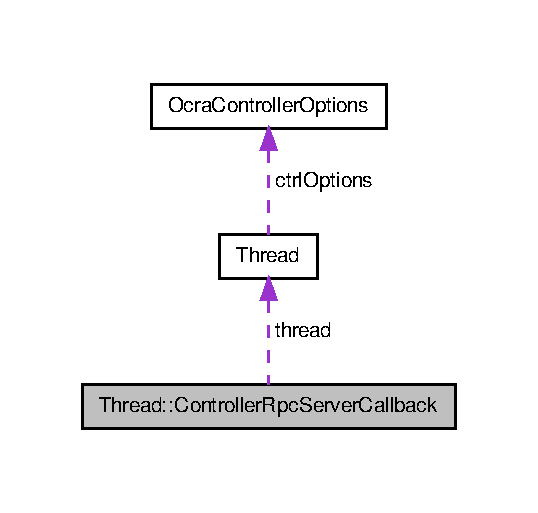
\includegraphics[width=258pt]{classThread_1_1ControllerRpcServerCallback__coll__graph}
\end{center}
\end{figure}
\subsection*{\-Public \-Member \-Functions}
\begin{DoxyCompactItemize}
\item 
\hyperlink{classThread_1_1ControllerRpcServerCallback_ad836e4cdaafc42ad309b5248ef38c280}{\-Controller\-Rpc\-Server\-Callback} (\hyperlink{classThread}{\-Thread} \&thread\-Ref)
\item 
virtual bool \hyperlink{classThread_1_1ControllerRpcServerCallback_a61f5510543f1bb96793dceca13eb6865}{read} (yarp\-::os\-::\-Connection\-Reader \&connection)
\end{DoxyCompactItemize}
\subsection*{\-Private \-Attributes}
\begin{DoxyCompactItemize}
\item 
\hyperlink{classThread}{\-Thread} \& \hyperlink{classThread_1_1ControllerRpcServerCallback_a466f100742fdac49e0016ec2f0c43536}{thread}
\end{DoxyCompactItemize}


\subsection{\-Detailed \-Description}
\-A callback function which binds the rpc server port opened in the contoller server module to the controller thread's parsing function. 

\subsection{\-Constructor \& \-Destructor \-Documentation}
\hypertarget{classThread_1_1ControllerRpcServerCallback_ad836e4cdaafc42ad309b5248ef38c280}{\index{\-Thread\-::\-Controller\-Rpc\-Server\-Callback@{\-Thread\-::\-Controller\-Rpc\-Server\-Callback}!\-Controller\-Rpc\-Server\-Callback@{\-Controller\-Rpc\-Server\-Callback}}
\index{\-Controller\-Rpc\-Server\-Callback@{\-Controller\-Rpc\-Server\-Callback}!Thread::ControllerRpcServerCallback@{\-Thread\-::\-Controller\-Rpc\-Server\-Callback}}
\subsubsection[{\-Controller\-Rpc\-Server\-Callback}]{\setlength{\rightskip}{0pt plus 5cm}{\bf \-Thread\-::\-Controller\-Rpc\-Server\-Callback\-::\-Controller\-Rpc\-Server\-Callback} (
\begin{DoxyParamCaption}
\item[{{\bf \-Thread} \&}]{thread\-Ref}
\end{DoxyParamCaption}
)}}\label{classThread_1_1ControllerRpcServerCallback_ad836e4cdaafc42ad309b5248ef38c280}
\-Constructor 
\begin{DoxyParams}{\-Parameters}
{\em ct\-Thread\-Ptr} & \-A shared pointer to the control thread. \\
\hline
\end{DoxyParams}


\subsection{\-Member \-Function \-Documentation}
\hypertarget{classThread_1_1ControllerRpcServerCallback_a61f5510543f1bb96793dceca13eb6865}{\index{\-Thread\-::\-Controller\-Rpc\-Server\-Callback@{\-Thread\-::\-Controller\-Rpc\-Server\-Callback}!read@{read}}
\index{read@{read}!Thread::ControllerRpcServerCallback@{\-Thread\-::\-Controller\-Rpc\-Server\-Callback}}
\subsubsection[{read}]{\setlength{\rightskip}{0pt plus 5cm}bool {\bf \-Thread\-::\-Controller\-Rpc\-Server\-Callback\-::read} (
\begin{DoxyParamCaption}
\item[{yarp\-::os\-::\-Connection\-Reader \&}]{connection}
\end{DoxyParamCaption}
)\hspace{0.3cm}{\ttfamily  \mbox{[}virtual\mbox{]}}}}\label{classThread_1_1ControllerRpcServerCallback_a61f5510543f1bb96793dceca13eb6865}
read 
\begin{DoxyParams}{\-Parameters}
{\em connection} & \-Reads a port connection.\\
\hline
\end{DoxyParams}
\begin{DoxyReturn}{\-Returns}
\-A boolean which tells whether or not a message was read. 
\end{DoxyReturn}


\subsection{\-Member \-Data \-Documentation}
\hypertarget{classThread_1_1ControllerRpcServerCallback_a466f100742fdac49e0016ec2f0c43536}{\index{\-Thread\-::\-Controller\-Rpc\-Server\-Callback@{\-Thread\-::\-Controller\-Rpc\-Server\-Callback}!thread@{thread}}
\index{thread@{thread}!Thread::ControllerRpcServerCallback@{\-Thread\-::\-Controller\-Rpc\-Server\-Callback}}
\subsubsection[{thread}]{\setlength{\rightskip}{0pt plus 5cm}{\bf \-Thread}\& {\bf \-Thread\-::\-Controller\-Rpc\-Server\-Callback\-::thread}\hspace{0.3cm}{\ttfamily  \mbox{[}private\mbox{]}}}}\label{classThread_1_1ControllerRpcServerCallback_a466f100742fdac49e0016ec2f0c43536}
\-A shared pointer to the control thread. 

\-The documentation for this class was generated from the following files\-:\begin{DoxyCompactItemize}
\item 
ocra-\/wbi-\/plugins/ocra-\/icub-\/server/include/ocra-\/icub-\/server/\hyperlink{Thread_8h}{\-Thread.\-h}\item 
ocra-\/wbi-\/plugins/ocra-\/icub-\/server/src/\hyperlink{Thread_8cpp}{\-Thread.\-cpp}\end{DoxyCompactItemize}

\hypertarget{classThread_1_1DebugRpcServerCallback}{\section{\-Thread\-:\-:\-Debug\-Rpc\-Server\-Callback \-Class \-Reference}
\label{classThread_1_1DebugRpcServerCallback}\index{\-Thread\-::\-Debug\-Rpc\-Server\-Callback@{\-Thread\-::\-Debug\-Rpc\-Server\-Callback}}
}


\-A callback function which binds the rpc server port opened in the contoller server module to the controller thread's parsing function.  




{\ttfamily \#include $<$\-Thread.\-h$>$}



\-Collaboration diagram for \-Thread\-:\-:\-Debug\-Rpc\-Server\-Callback\-:\nopagebreak
\begin{figure}[H]
\begin{center}
\leavevmode
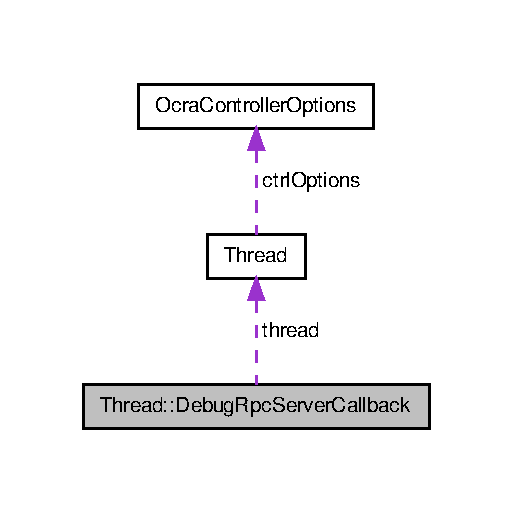
\includegraphics[width=246pt]{classThread_1_1DebugRpcServerCallback__coll__graph}
\end{center}
\end{figure}
\subsection*{\-Public \-Member \-Functions}
\begin{DoxyCompactItemize}
\item 
\hyperlink{classThread_1_1DebugRpcServerCallback_a479142cdf2f840df23b4605a532aaddf}{\-Debug\-Rpc\-Server\-Callback} (\hyperlink{classThread}{\-Thread} \&thread\-Ref)
\item 
virtual bool \hyperlink{classThread_1_1DebugRpcServerCallback_a3b39ac9b379ce3212bb2b05a89fa6024}{read} (yarp\-::os\-::\-Connection\-Reader \&connection)
\end{DoxyCompactItemize}
\subsection*{\-Private \-Attributes}
\begin{DoxyCompactItemize}
\item 
\hyperlink{classThread}{\-Thread} \& \hyperlink{classThread_1_1DebugRpcServerCallback_ad75683fc200019e8f681ad441b6ce84b}{thread}
\end{DoxyCompactItemize}


\subsection{\-Detailed \-Description}
\-A callback function which binds the rpc server port opened in the contoller server module to the controller thread's parsing function. 

\subsection{\-Constructor \& \-Destructor \-Documentation}
\hypertarget{classThread_1_1DebugRpcServerCallback_a479142cdf2f840df23b4605a532aaddf}{\index{\-Thread\-::\-Debug\-Rpc\-Server\-Callback@{\-Thread\-::\-Debug\-Rpc\-Server\-Callback}!\-Debug\-Rpc\-Server\-Callback@{\-Debug\-Rpc\-Server\-Callback}}
\index{\-Debug\-Rpc\-Server\-Callback@{\-Debug\-Rpc\-Server\-Callback}!Thread::DebugRpcServerCallback@{\-Thread\-::\-Debug\-Rpc\-Server\-Callback}}
\subsubsection[{\-Debug\-Rpc\-Server\-Callback}]{\setlength{\rightskip}{0pt plus 5cm}{\bf \-Thread\-::\-Debug\-Rpc\-Server\-Callback\-::\-Debug\-Rpc\-Server\-Callback} (
\begin{DoxyParamCaption}
\item[{{\bf \-Thread} \&}]{thread\-Ref}
\end{DoxyParamCaption}
)}}\label{classThread_1_1DebugRpcServerCallback_a479142cdf2f840df23b4605a532aaddf}
\-Constructor 
\begin{DoxyParams}{\-Parameters}
{\em ct\-Thread\-Ptr} & \-A shared pointer to the control thread. \\
\hline
\end{DoxyParams}


\subsection{\-Member \-Function \-Documentation}
\hypertarget{classThread_1_1DebugRpcServerCallback_a3b39ac9b379ce3212bb2b05a89fa6024}{\index{\-Thread\-::\-Debug\-Rpc\-Server\-Callback@{\-Thread\-::\-Debug\-Rpc\-Server\-Callback}!read@{read}}
\index{read@{read}!Thread::DebugRpcServerCallback@{\-Thread\-::\-Debug\-Rpc\-Server\-Callback}}
\subsubsection[{read}]{\setlength{\rightskip}{0pt plus 5cm}bool {\bf \-Thread\-::\-Debug\-Rpc\-Server\-Callback\-::read} (
\begin{DoxyParamCaption}
\item[{yarp\-::os\-::\-Connection\-Reader \&}]{connection}
\end{DoxyParamCaption}
)\hspace{0.3cm}{\ttfamily  \mbox{[}virtual\mbox{]}}}}\label{classThread_1_1DebugRpcServerCallback_a3b39ac9b379ce3212bb2b05a89fa6024}
read 
\begin{DoxyParams}{\-Parameters}
{\em connection} & \-Reads a port connection.\\
\hline
\end{DoxyParams}
\begin{DoxyReturn}{\-Returns}
\-A boolean which tells whether or not a message was read. 
\end{DoxyReturn}


\subsection{\-Member \-Data \-Documentation}
\hypertarget{classThread_1_1DebugRpcServerCallback_ad75683fc200019e8f681ad441b6ce84b}{\index{\-Thread\-::\-Debug\-Rpc\-Server\-Callback@{\-Thread\-::\-Debug\-Rpc\-Server\-Callback}!thread@{thread}}
\index{thread@{thread}!Thread::DebugRpcServerCallback@{\-Thread\-::\-Debug\-Rpc\-Server\-Callback}}
\subsubsection[{thread}]{\setlength{\rightskip}{0pt plus 5cm}{\bf \-Thread}\& {\bf \-Thread\-::\-Debug\-Rpc\-Server\-Callback\-::thread}\hspace{0.3cm}{\ttfamily  \mbox{[}private\mbox{]}}}}\label{classThread_1_1DebugRpcServerCallback_ad75683fc200019e8f681ad441b6ce84b}
\-A shared pointer to the control thread. 

\-The documentation for this class was generated from the following files\-:\begin{DoxyCompactItemize}
\item 
ocra-\/wbi-\/plugins/ocra-\/icub-\/server/include/ocra-\/icub-\/server/\hyperlink{Thread_8h}{\-Thread.\-h}\item 
ocra-\/wbi-\/plugins/ocra-\/icub-\/server/src/\hyperlink{Thread_8cpp}{\-Thread.\-cpp}\end{DoxyCompactItemize}

\hypertarget{classExampleClient}{\section{\-Example\-Client \-Class \-Reference}
\label{classExampleClient}\index{\-Example\-Client@{\-Example\-Client}}
}


{\ttfamily \#include $<$\-Example\-Client.\-h$>$}

\subsection*{\-Public \-Member \-Functions}
\begin{DoxyCompactItemize}
\item 
\hyperlink{classExampleClient_aed7d851662cba1484ecf1db8161d6e62}{\-Example\-Client} (std\-::shared\-\_\-ptr$<$ ocra\-::\-Model $>$ model\-Ptr, const int loop\-Period)
\item 
virtual \hyperlink{classExampleClient_abdca7dbe5fdab81d7d661a677e5ccd14}{$\sim$\-Example\-Client} ()
\end{DoxyCompactItemize}
\subsection*{\-Protected \-Member \-Functions}
\begin{DoxyCompactItemize}
\item 
virtual bool \hyperlink{classExampleClient_ad504d1d87997fc95bfeca6aa925a4fa6}{initialize} ()
\item 
virtual void \hyperlink{classExampleClient_a5acf25784c1c5b51c2c085327f195002}{release} ()
\item 
virtual void \hyperlink{classExampleClient_afb58f3425aafe2d4c38195cb3c667dbc}{loop} ()
\end{DoxyCompactItemize}
\subsection*{\-Private \-Attributes}
\begin{DoxyCompactItemize}
\item 
double \hyperlink{classExampleClient_aaa5ec782e9aaa1e94d7182872f743c02}{start\-Time}
\item 
double \hyperlink{classExampleClient_acade7035d4e39290cbda08b98249a629}{wait\-Time}
\item 
bool \hyperlink{classExampleClient_a90ce0c4d970c903b3e6afb6f5ca2a228}{trigger}
\item 
bool \hyperlink{classExampleClient_acd2cf0f0479ff8bbf5b64924d83beb60}{done}
\item 
\-Eigen\-::\-Matrix\-Xd \hyperlink{classExampleClient_acf4657277ecb08168d9a17c208814823}{waypoints}
\item 
std\-::shared\-\_\-ptr\*
$<$ ocra\-\_\-recipes\-::\-Trajectory\-Thread $>$ \hyperlink{classExampleClient_a4311b0e8c4878c23df2b5ba048d8bc05}{left\-Hand\-Traj\-Thread}
\item 
bool \hyperlink{classExampleClient_a7fb2b50cbdac0ec3a32e44b5bbc3b11f}{p1}
\item 
bool \hyperlink{classExampleClient_a07c2bc5c5c522e77a726017c28db2ec9}{p2}
\item 
bool \hyperlink{classExampleClient_ab41df6f34a51e649051adbac6d3077f9}{p3}
\end{DoxyCompactItemize}


\subsection{\-Constructor \& \-Destructor \-Documentation}
\hypertarget{classExampleClient_aed7d851662cba1484ecf1db8161d6e62}{\index{\-Example\-Client@{\-Example\-Client}!\-Example\-Client@{\-Example\-Client}}
\index{\-Example\-Client@{\-Example\-Client}!ExampleClient@{\-Example\-Client}}
\subsubsection[{\-Example\-Client}]{\setlength{\rightskip}{0pt plus 5cm}{\bf \-Example\-Client\-::\-Example\-Client} (
\begin{DoxyParamCaption}
\item[{std\-::shared\-\_\-ptr$<$ ocra\-::\-Model $>$}]{model\-Ptr, }
\item[{const int}]{loop\-Period}
\end{DoxyParamCaption}
)}}\label{classExampleClient_aed7d851662cba1484ecf1db8161d6e62}
\hypertarget{classExampleClient_abdca7dbe5fdab81d7d661a677e5ccd14}{\index{\-Example\-Client@{\-Example\-Client}!$\sim$\-Example\-Client@{$\sim$\-Example\-Client}}
\index{$\sim$\-Example\-Client@{$\sim$\-Example\-Client}!ExampleClient@{\-Example\-Client}}
\subsubsection[{$\sim$\-Example\-Client}]{\setlength{\rightskip}{0pt plus 5cm}{\bf \-Example\-Client\-::$\sim$\-Example\-Client} (
\begin{DoxyParamCaption}
{}
\end{DoxyParamCaption}
)\hspace{0.3cm}{\ttfamily  \mbox{[}virtual\mbox{]}}}}\label{classExampleClient_abdca7dbe5fdab81d7d661a677e5ccd14}


\subsection{\-Member \-Function \-Documentation}
\hypertarget{classExampleClient_ad504d1d87997fc95bfeca6aa925a4fa6}{\index{\-Example\-Client@{\-Example\-Client}!initialize@{initialize}}
\index{initialize@{initialize}!ExampleClient@{\-Example\-Client}}
\subsubsection[{initialize}]{\setlength{\rightskip}{0pt plus 5cm}bool {\bf \-Example\-Client\-::initialize} (
\begin{DoxyParamCaption}
{}
\end{DoxyParamCaption}
)\hspace{0.3cm}{\ttfamily  \mbox{[}protected, virtual\mbox{]}}}}\label{classExampleClient_ad504d1d87997fc95bfeca6aa925a4fa6}
\hypertarget{classExampleClient_afb58f3425aafe2d4c38195cb3c667dbc}{\index{\-Example\-Client@{\-Example\-Client}!loop@{loop}}
\index{loop@{loop}!ExampleClient@{\-Example\-Client}}
\subsubsection[{loop}]{\setlength{\rightskip}{0pt plus 5cm}void {\bf \-Example\-Client\-::loop} (
\begin{DoxyParamCaption}
{}
\end{DoxyParamCaption}
)\hspace{0.3cm}{\ttfamily  \mbox{[}protected, virtual\mbox{]}}}}\label{classExampleClient_afb58f3425aafe2d4c38195cb3c667dbc}
\hypertarget{classExampleClient_a5acf25784c1c5b51c2c085327f195002}{\index{\-Example\-Client@{\-Example\-Client}!release@{release}}
\index{release@{release}!ExampleClient@{\-Example\-Client}}
\subsubsection[{release}]{\setlength{\rightskip}{0pt plus 5cm}void {\bf \-Example\-Client\-::release} (
\begin{DoxyParamCaption}
{}
\end{DoxyParamCaption}
)\hspace{0.3cm}{\ttfamily  \mbox{[}protected, virtual\mbox{]}}}}\label{classExampleClient_a5acf25784c1c5b51c2c085327f195002}


\subsection{\-Member \-Data \-Documentation}
\hypertarget{classExampleClient_acd2cf0f0479ff8bbf5b64924d83beb60}{\index{\-Example\-Client@{\-Example\-Client}!done@{done}}
\index{done@{done}!ExampleClient@{\-Example\-Client}}
\subsubsection[{done}]{\setlength{\rightskip}{0pt plus 5cm}bool {\bf \-Example\-Client\-::done}\hspace{0.3cm}{\ttfamily  \mbox{[}private\mbox{]}}}}\label{classExampleClient_acd2cf0f0479ff8bbf5b64924d83beb60}
\hypertarget{classExampleClient_a4311b0e8c4878c23df2b5ba048d8bc05}{\index{\-Example\-Client@{\-Example\-Client}!left\-Hand\-Traj\-Thread@{left\-Hand\-Traj\-Thread}}
\index{left\-Hand\-Traj\-Thread@{left\-Hand\-Traj\-Thread}!ExampleClient@{\-Example\-Client}}
\subsubsection[{left\-Hand\-Traj\-Thread}]{\setlength{\rightskip}{0pt plus 5cm}std\-::shared\-\_\-ptr$<$ocra\-\_\-recipes\-::\-Trajectory\-Thread$>$ {\bf \-Example\-Client\-::left\-Hand\-Traj\-Thread}\hspace{0.3cm}{\ttfamily  \mbox{[}private\mbox{]}}}}\label{classExampleClient_a4311b0e8c4878c23df2b5ba048d8bc05}
\hypertarget{classExampleClient_a7fb2b50cbdac0ec3a32e44b5bbc3b11f}{\index{\-Example\-Client@{\-Example\-Client}!p1@{p1}}
\index{p1@{p1}!ExampleClient@{\-Example\-Client}}
\subsubsection[{p1}]{\setlength{\rightskip}{0pt plus 5cm}bool {\bf \-Example\-Client\-::p1}\hspace{0.3cm}{\ttfamily  \mbox{[}private\mbox{]}}}}\label{classExampleClient_a7fb2b50cbdac0ec3a32e44b5bbc3b11f}
\hypertarget{classExampleClient_a07c2bc5c5c522e77a726017c28db2ec9}{\index{\-Example\-Client@{\-Example\-Client}!p2@{p2}}
\index{p2@{p2}!ExampleClient@{\-Example\-Client}}
\subsubsection[{p2}]{\setlength{\rightskip}{0pt plus 5cm}bool {\bf \-Example\-Client\-::p2}\hspace{0.3cm}{\ttfamily  \mbox{[}private\mbox{]}}}}\label{classExampleClient_a07c2bc5c5c522e77a726017c28db2ec9}
\hypertarget{classExampleClient_ab41df6f34a51e649051adbac6d3077f9}{\index{\-Example\-Client@{\-Example\-Client}!p3@{p3}}
\index{p3@{p3}!ExampleClient@{\-Example\-Client}}
\subsubsection[{p3}]{\setlength{\rightskip}{0pt plus 5cm}bool {\bf \-Example\-Client\-::p3}\hspace{0.3cm}{\ttfamily  \mbox{[}private\mbox{]}}}}\label{classExampleClient_ab41df6f34a51e649051adbac6d3077f9}
\hypertarget{classExampleClient_aaa5ec782e9aaa1e94d7182872f743c02}{\index{\-Example\-Client@{\-Example\-Client}!start\-Time@{start\-Time}}
\index{start\-Time@{start\-Time}!ExampleClient@{\-Example\-Client}}
\subsubsection[{start\-Time}]{\setlength{\rightskip}{0pt plus 5cm}double {\bf \-Example\-Client\-::start\-Time}\hspace{0.3cm}{\ttfamily  \mbox{[}private\mbox{]}}}}\label{classExampleClient_aaa5ec782e9aaa1e94d7182872f743c02}
\hypertarget{classExampleClient_a90ce0c4d970c903b3e6afb6f5ca2a228}{\index{\-Example\-Client@{\-Example\-Client}!trigger@{trigger}}
\index{trigger@{trigger}!ExampleClient@{\-Example\-Client}}
\subsubsection[{trigger}]{\setlength{\rightskip}{0pt plus 5cm}bool {\bf \-Example\-Client\-::trigger}\hspace{0.3cm}{\ttfamily  \mbox{[}private\mbox{]}}}}\label{classExampleClient_a90ce0c4d970c903b3e6afb6f5ca2a228}
\hypertarget{classExampleClient_acade7035d4e39290cbda08b98249a629}{\index{\-Example\-Client@{\-Example\-Client}!wait\-Time@{wait\-Time}}
\index{wait\-Time@{wait\-Time}!ExampleClient@{\-Example\-Client}}
\subsubsection[{wait\-Time}]{\setlength{\rightskip}{0pt plus 5cm}double {\bf \-Example\-Client\-::wait\-Time}\hspace{0.3cm}{\ttfamily  \mbox{[}private\mbox{]}}}}\label{classExampleClient_acade7035d4e39290cbda08b98249a629}
\hypertarget{classExampleClient_acf4657277ecb08168d9a17c208814823}{\index{\-Example\-Client@{\-Example\-Client}!waypoints@{waypoints}}
\index{waypoints@{waypoints}!ExampleClient@{\-Example\-Client}}
\subsubsection[{waypoints}]{\setlength{\rightskip}{0pt plus 5cm}\-Eigen\-::\-Matrix\-Xd {\bf \-Example\-Client\-::waypoints}\hspace{0.3cm}{\ttfamily  \mbox{[}private\mbox{]}}}}\label{classExampleClient_acf4657277ecb08168d9a17c208814823}


\-The documentation for this class was generated from the following files\-:\begin{DoxyCompactItemize}
\item 
ocra-\/wbi-\/plugins/ocra-\/icub-\/clients/example-\/client/include/example-\/client/\hyperlink{ExampleClient_8h}{\-Example\-Client.\-h}\item 
ocra-\/wbi-\/plugins/ocra-\/icub-\/clients/example-\/client/src/\hyperlink{ExampleClient_8cpp}{\-Example\-Client.\-cpp}\end{DoxyCompactItemize}

\hypertarget{classIcubControllerServer}{\section{\-Icub\-Controller\-Server \-Class \-Reference}
\label{classIcubControllerServer}\index{\-Icub\-Controller\-Server@{\-Icub\-Controller\-Server}}
}


{\ttfamily \#include $<$\-Icub\-Controller\-Server.\-h$>$}

\subsection*{\-Public \-Member \-Functions}
\begin{DoxyCompactItemize}
\item 
\hyperlink{classIcubControllerServer_a6b0a6021e3c82e72ac97ad30d3f0c082}{\-Icub\-Controller\-Server} (std\-::shared\-\_\-ptr$<$ wbi\-::whole\-Body\-Interface $>$ robot, std\-::string icub\-Name, const bool using\-Floating\-Base, const ocra\-\_\-recipes\-::\-C\-O\-N\-T\-R\-O\-L\-L\-E\-R\-\_\-\-T\-Y\-P\-E ctrl\-Type=ocra\-\_\-recipes\-::\-W\-O\-C\-R\-A\-\_\-\-C\-O\-N\-T\-R\-O\-L\-L\-E\-R, const ocra\-\_\-recipes\-::\-S\-O\-L\-V\-E\-R\-\_\-\-T\-Y\-P\-E solver=ocra\-\_\-recipes\-::\-Q\-U\-A\-D\-P\-R\-O\-G, const bool using\-Interprocess\-Communication=true, const bool \hyperlink{classIcubControllerServer_adc410f503b14ed288c01e877ac405114}{use\-Odometry}=false)
\item 
virtual \hyperlink{classIcubControllerServer_a7582d4bbf9851ee9b58913ea2a89e5fd}{$\sim$\-Icub\-Controller\-Server} ()
\item 
virtual ocra\-::\-Model\-::\-Ptr \hyperlink{classIcubControllerServer_a025d8e257a69ef3d2c5a10b3cbfe2350}{load\-Robot\-Model} ()
\item 
virtual void \hyperlink{classIcubControllerServer_ac068c7930f342bb0cb0969d0d04267cf}{get\-Robot\-State} (\-Eigen\-::\-Vector\-Xd \&q, \-Eigen\-::\-Vector\-Xd \&qd, \-Eigen\-::\-Displacementd \&\-H\-\_\-root, \-Eigen\-::\-Twistd \&\-T\-\_\-root)
\item 
bool \hyperlink{classIcubControllerServer_a810f139a27e06458549ccbb3fde12359}{initialize\-Odometry} (std\-::string model\-\_\-file, std\-::string initial\-Fixed\-Frame)
\item 
std\-::vector$<$ std\-::string $>$ \hyperlink{classIcubControllerServer_a892bb43e568d3f112465dff1e0c6b348}{get\-Canonical\-\_\-i\-Cub\-Joints} ()
\item 
void \hyperlink{classIcubControllerServer_a032c035880f8ec2b77ef14521be6e75a}{root\-Frame\-Velocity} (\-Eigen\-::\-Vector\-Xd \&q, \-Eigen\-::\-Vector\-Xd \&qd, i\-Dyn\-Tree\-::\-Transform \&wbi\-\_\-\-H\-\_\-root\-\_\-\-Transform, double regularization, int \-L\-E\-F\-T\-\_\-\-F\-O\-O\-T\-\_\-\-C\-O\-N\-T\-A\-C\-T, int \-R\-I\-G\-H\-T\-\_\-\-F\-O\-O\-T\-\_\-\-C\-O\-N\-T\-A\-C\-T, \-Eigen\-::\-Vector\-Xd \&twist)
\item 
void \hyperlink{classIcubControllerServer_a27211ecba9fc8618733bcaea9ff7d140}{root\-Frame\-Velocity\-Piv\-L\-U} (\-Eigen\-::\-Vector\-Xd \&q, \-Eigen\-::\-Vector\-Xd \&qd, i\-Dyn\-Tree\-::\-Transform \&wbi\-\_\-\-H\-\_\-root\-\_\-\-Transform, \-Eigen\-::\-Vector\-Xd \&twist)
\item 
void \hyperlink{classIcubControllerServer_a82650f373c3c2c52a91cc744c67b0dcf}{root\-Frame\-Velocity\-Piv\-L\-U} (\-Eigen\-::\-Vector\-Xd \&q, \-Eigen\-::\-Vector\-Xd \&qd, i\-Dyn\-Tree\-::\-Transform \&wbi\-\_\-\-H\-\_\-root\-\_\-\-Transform, int \-L\-E\-F\-T\-\_\-\-F\-O\-O\-T\-\_\-\-C\-O\-N\-T\-A\-C\-T, int \-R\-I\-G\-H\-T\-\_\-\-F\-O\-O\-T\-\_\-\-C\-O\-N\-T\-A\-C\-T, \-Eigen\-::\-Vector\-Xd \&twist)
\item 
void \hyperlink{classIcubControllerServer_a0132b1ddc3dafd29506e4684ea42cf58}{pinv} (\-Eigen\-::\-Matrix\-Xd mat, \-Eigen\-::\-Matrix\-Xd \&pinvmat, double pinvtoler=1.\-0e-\/6) const 
\item 
void \hyperlink{classIcubControllerServer_aaedff28c5d9ac9a7cdbc24c9e0cbc5b3}{velocity\-Error} (\-Eigen\-::\-Matrix\-Xd \-A, \-Eigen\-::\-Matrix\-Xd \-B, \-Eigen\-::\-Matrix\-Xd \-X)
\end{DoxyCompactItemize}
\subsection*{\-Private \-Attributes}
\begin{DoxyCompactItemize}
\item 
std\-::shared\-\_\-ptr\*
$<$ wbi\-::whole\-Body\-Interface $>$ \hyperlink{classIcubControllerServer_ae8a89707675adb58bb3006bc085828b7}{wbi}
\item 
std\-::string \hyperlink{classIcubControllerServer_a041d6687258c36677914b1d15f18e153}{robot\-Name}
\item 
bool \hyperlink{classIcubControllerServer_aebc2019921c3eabb53c01012fbd2355a}{is\-Floating\-Base}
\item 
bool \hyperlink{classIcubControllerServer_adc410f503b14ed288c01e877ac405114}{use\-Odometry}
\item 
int \hyperlink{classIcubControllerServer_ab5fb1f18775cfe3036894c73dc21ebcf}{n\-Do\-F}
\item 
\-Eigen\-::\-Vector\-Xd \hyperlink{classIcubControllerServer_a42f6a8db660da9dbafbc57941b1ee12f}{wbi\-\_\-\-H\-\_\-root\-\_\-\-Vector}
\item 
\-Eigen\-::\-Vector\-Xd \hyperlink{classIcubControllerServer_a818b66e75b7f9457a6a5bcbb3c1306a7}{wbi\-\_\-\-T\-\_\-root\-\_\-\-Vector}
\item 
wbi\-::\-Frame \hyperlink{classIcubControllerServer_afd983b69c043eedf958e53582b22195a}{wbi\-\_\-\-H\-\_\-root}
\item 
i\-Dyn\-Tree\-::\-Simple\-Legged\-Odometry \hyperlink{classIcubControllerServer_ad0484106ab9d7fd42e2bd682338871c7}{odometry}
\end{DoxyCompactItemize}
\subsection*{\-Static \-Private \-Attributes}
\begin{DoxyCompactItemize}
\item 
static const int \hyperlink{classIcubControllerServer_aa977ca558c184e4331121522cc58d2e7}{\-A\-L\-L\-\_\-\-J\-O\-I\-N\-T\-S} = -\/1
\end{DoxyCompactItemize}


\subsection{\-Constructor \& \-Destructor \-Documentation}
\hypertarget{classIcubControllerServer_a6b0a6021e3c82e72ac97ad30d3f0c082}{\index{\-Icub\-Controller\-Server@{\-Icub\-Controller\-Server}!\-Icub\-Controller\-Server@{\-Icub\-Controller\-Server}}
\index{\-Icub\-Controller\-Server@{\-Icub\-Controller\-Server}!IcubControllerServer@{\-Icub\-Controller\-Server}}
\subsubsection[{\-Icub\-Controller\-Server}]{\setlength{\rightskip}{0pt plus 5cm}{\bf \-Icub\-Controller\-Server\-::\-Icub\-Controller\-Server} (
\begin{DoxyParamCaption}
\item[{std\-::shared\-\_\-ptr$<$ wbi\-::whole\-Body\-Interface $>$}]{robot, }
\item[{std\-::string}]{icub\-Name, }
\item[{const bool}]{using\-Floating\-Base, }
\item[{const ocra\-\_\-recipes\-::\-C\-O\-N\-T\-R\-O\-L\-L\-E\-R\-\_\-\-T\-Y\-P\-E}]{ctrl\-Type = {\ttfamily ocra\-\_\-recipes\-:\-:\-W\-O\-C\-R\-A\-\_\-\-C\-O\-N\-T\-R\-O\-L\-L\-E\-R}, }
\item[{const ocra\-\_\-recipes\-::\-S\-O\-L\-V\-E\-R\-\_\-\-T\-Y\-P\-E}]{solver = {\ttfamily ocra\-\_\-recipes\-:\-:\-Q\-U\-A\-D\-P\-R\-O\-G}, }
\item[{const bool}]{using\-Interprocess\-Communication = {\ttfamily true}, }
\item[{const bool}]{use\-Odometry = {\ttfamily false}}
\end{DoxyParamCaption}
)}}\label{classIcubControllerServer_a6b0a6021e3c82e72ac97ad30d3f0c082}
\hypertarget{classIcubControllerServer_a7582d4bbf9851ee9b58913ea2a89e5fd}{\index{\-Icub\-Controller\-Server@{\-Icub\-Controller\-Server}!$\sim$\-Icub\-Controller\-Server@{$\sim$\-Icub\-Controller\-Server}}
\index{$\sim$\-Icub\-Controller\-Server@{$\sim$\-Icub\-Controller\-Server}!IcubControllerServer@{\-Icub\-Controller\-Server}}
\subsubsection[{$\sim$\-Icub\-Controller\-Server}]{\setlength{\rightskip}{0pt plus 5cm}{\bf \-Icub\-Controller\-Server\-::$\sim$\-Icub\-Controller\-Server} (
\begin{DoxyParamCaption}
{}
\end{DoxyParamCaption}
)\hspace{0.3cm}{\ttfamily  \mbox{[}virtual\mbox{]}}}}\label{classIcubControllerServer_a7582d4bbf9851ee9b58913ea2a89e5fd}


\subsection{\-Member \-Function \-Documentation}
\hypertarget{classIcubControllerServer_a892bb43e568d3f112465dff1e0c6b348}{\index{\-Icub\-Controller\-Server@{\-Icub\-Controller\-Server}!get\-Canonical\-\_\-i\-Cub\-Joints@{get\-Canonical\-\_\-i\-Cub\-Joints}}
\index{get\-Canonical\-\_\-i\-Cub\-Joints@{get\-Canonical\-\_\-i\-Cub\-Joints}!IcubControllerServer@{\-Icub\-Controller\-Server}}
\subsubsection[{get\-Canonical\-\_\-i\-Cub\-Joints}]{\setlength{\rightskip}{0pt plus 5cm}std\-::vector$<$ std\-::string $>$ {\bf \-Icub\-Controller\-Server\-::get\-Canonical\-\_\-i\-Cub\-Joints} (
\begin{DoxyParamCaption}
{}
\end{DoxyParamCaption}
)}}\label{classIcubControllerServer_a892bb43e568d3f112465dff1e0c6b348}
\hypertarget{classIcubControllerServer_ac068c7930f342bb0cb0969d0d04267cf}{\index{\-Icub\-Controller\-Server@{\-Icub\-Controller\-Server}!get\-Robot\-State@{get\-Robot\-State}}
\index{get\-Robot\-State@{get\-Robot\-State}!IcubControllerServer@{\-Icub\-Controller\-Server}}
\subsubsection[{get\-Robot\-State}]{\setlength{\rightskip}{0pt plus 5cm}void {\bf \-Icub\-Controller\-Server\-::get\-Robot\-State} (
\begin{DoxyParamCaption}
\item[{\-Eigen\-::\-Vector\-Xd \&}]{q, }
\item[{\-Eigen\-::\-Vector\-Xd \&}]{qd, }
\item[{\-Eigen\-::\-Displacementd \&}]{\-H\-\_\-root, }
\item[{\-Eigen\-::\-Twistd \&}]{\-T\-\_\-root}
\end{DoxyParamCaption}
)\hspace{0.3cm}{\ttfamily  \mbox{[}virtual\mbox{]}}}}\label{classIcubControllerServer_ac068c7930f342bb0cb0969d0d04267cf}
\hypertarget{classIcubControllerServer_a810f139a27e06458549ccbb3fde12359}{\index{\-Icub\-Controller\-Server@{\-Icub\-Controller\-Server}!initialize\-Odometry@{initialize\-Odometry}}
\index{initialize\-Odometry@{initialize\-Odometry}!IcubControllerServer@{\-Icub\-Controller\-Server}}
\subsubsection[{initialize\-Odometry}]{\setlength{\rightskip}{0pt plus 5cm}bool {\bf \-Icub\-Controller\-Server\-::initialize\-Odometry} (
\begin{DoxyParamCaption}
\item[{std\-::string}]{model\-\_\-file, }
\item[{std\-::string}]{initial\-Fixed\-Frame}
\end{DoxyParamCaption}
)}}\label{classIcubControllerServer_a810f139a27e06458549ccbb3fde12359}
\hypertarget{classIcubControllerServer_a025d8e257a69ef3d2c5a10b3cbfe2350}{\index{\-Icub\-Controller\-Server@{\-Icub\-Controller\-Server}!load\-Robot\-Model@{load\-Robot\-Model}}
\index{load\-Robot\-Model@{load\-Robot\-Model}!IcubControllerServer@{\-Icub\-Controller\-Server}}
\subsubsection[{load\-Robot\-Model}]{\setlength{\rightskip}{0pt plus 5cm}ocra\-::\-Model\-::\-Ptr {\bf \-Icub\-Controller\-Server\-::load\-Robot\-Model} (
\begin{DoxyParamCaption}
{}
\end{DoxyParamCaption}
)\hspace{0.3cm}{\ttfamily  \mbox{[}virtual\mbox{]}}}}\label{classIcubControllerServer_a025d8e257a69ef3d2c5a10b3cbfe2350}
\hypertarget{classIcubControllerServer_a0132b1ddc3dafd29506e4684ea42cf58}{\index{\-Icub\-Controller\-Server@{\-Icub\-Controller\-Server}!pinv@{pinv}}
\index{pinv@{pinv}!IcubControllerServer@{\-Icub\-Controller\-Server}}
\subsubsection[{pinv}]{\setlength{\rightskip}{0pt plus 5cm}void {\bf \-Icub\-Controller\-Server\-::pinv} (
\begin{DoxyParamCaption}
\item[{\-Eigen\-::\-Matrix\-Xd}]{mat, }
\item[{\-Eigen\-::\-Matrix\-Xd \&}]{pinvmat, }
\item[{double}]{pinvtoler = {\ttfamily 1.0e-\/6}}
\end{DoxyParamCaption}
) const}}\label{classIcubControllerServer_a0132b1ddc3dafd29506e4684ea42cf58}
\hypertarget{classIcubControllerServer_a032c035880f8ec2b77ef14521be6e75a}{\index{\-Icub\-Controller\-Server@{\-Icub\-Controller\-Server}!root\-Frame\-Velocity@{root\-Frame\-Velocity}}
\index{root\-Frame\-Velocity@{root\-Frame\-Velocity}!IcubControllerServer@{\-Icub\-Controller\-Server}}
\subsubsection[{root\-Frame\-Velocity}]{\setlength{\rightskip}{0pt plus 5cm}void {\bf \-Icub\-Controller\-Server\-::root\-Frame\-Velocity} (
\begin{DoxyParamCaption}
\item[{\-Eigen\-::\-Vector\-Xd \&}]{q, }
\item[{\-Eigen\-::\-Vector\-Xd \&}]{qd, }
\item[{i\-Dyn\-Tree\-::\-Transform \&}]{wbi\-\_\-\-H\-\_\-root\-\_\-\-Transform, }
\item[{double}]{regularization, }
\item[{int}]{\-L\-E\-F\-T\-\_\-\-F\-O\-O\-T\-\_\-\-C\-O\-N\-T\-A\-C\-T, }
\item[{int}]{\-R\-I\-G\-H\-T\-\_\-\-F\-O\-O\-T\-\_\-\-C\-O\-N\-T\-A\-C\-T, }
\item[{\-Eigen\-::\-Vector\-Xd \&}]{twist}
\end{DoxyParamCaption}
)}}\label{classIcubControllerServer_a032c035880f8ec2b77ef14521be6e75a}
\hypertarget{classIcubControllerServer_a27211ecba9fc8618733bcaea9ff7d140}{\index{\-Icub\-Controller\-Server@{\-Icub\-Controller\-Server}!root\-Frame\-Velocity\-Piv\-L\-U@{root\-Frame\-Velocity\-Piv\-L\-U}}
\index{root\-Frame\-Velocity\-Piv\-L\-U@{root\-Frame\-Velocity\-Piv\-L\-U}!IcubControllerServer@{\-Icub\-Controller\-Server}}
\subsubsection[{root\-Frame\-Velocity\-Piv\-L\-U}]{\setlength{\rightskip}{0pt plus 5cm}void {\bf \-Icub\-Controller\-Server\-::root\-Frame\-Velocity\-Piv\-L\-U} (
\begin{DoxyParamCaption}
\item[{\-Eigen\-::\-Vector\-Xd \&}]{q, }
\item[{\-Eigen\-::\-Vector\-Xd \&}]{qd, }
\item[{i\-Dyn\-Tree\-::\-Transform \&}]{wbi\-\_\-\-H\-\_\-root\-\_\-\-Transform, }
\item[{\-Eigen\-::\-Vector\-Xd \&}]{twist}
\end{DoxyParamCaption}
)}}\label{classIcubControllerServer_a27211ecba9fc8618733bcaea9ff7d140}
\hypertarget{classIcubControllerServer_a82650f373c3c2c52a91cc744c67b0dcf}{\index{\-Icub\-Controller\-Server@{\-Icub\-Controller\-Server}!root\-Frame\-Velocity\-Piv\-L\-U@{root\-Frame\-Velocity\-Piv\-L\-U}}
\index{root\-Frame\-Velocity\-Piv\-L\-U@{root\-Frame\-Velocity\-Piv\-L\-U}!IcubControllerServer@{\-Icub\-Controller\-Server}}
\subsubsection[{root\-Frame\-Velocity\-Piv\-L\-U}]{\setlength{\rightskip}{0pt plus 5cm}void {\bf \-Icub\-Controller\-Server\-::root\-Frame\-Velocity\-Piv\-L\-U} (
\begin{DoxyParamCaption}
\item[{\-Eigen\-::\-Vector\-Xd \&}]{q, }
\item[{\-Eigen\-::\-Vector\-Xd \&}]{qd, }
\item[{i\-Dyn\-Tree\-::\-Transform \&}]{wbi\-\_\-\-H\-\_\-root\-\_\-\-Transform, }
\item[{int}]{\-L\-E\-F\-T\-\_\-\-F\-O\-O\-T\-\_\-\-C\-O\-N\-T\-A\-C\-T, }
\item[{int}]{\-R\-I\-G\-H\-T\-\_\-\-F\-O\-O\-T\-\_\-\-C\-O\-N\-T\-A\-C\-T, }
\item[{\-Eigen\-::\-Vector\-Xd \&}]{twist}
\end{DoxyParamCaption}
)}}\label{classIcubControllerServer_a82650f373c3c2c52a91cc744c67b0dcf}
\hypertarget{classIcubControllerServer_aaedff28c5d9ac9a7cdbc24c9e0cbc5b3}{\index{\-Icub\-Controller\-Server@{\-Icub\-Controller\-Server}!velocity\-Error@{velocity\-Error}}
\index{velocity\-Error@{velocity\-Error}!IcubControllerServer@{\-Icub\-Controller\-Server}}
\subsubsection[{velocity\-Error}]{\setlength{\rightskip}{0pt plus 5cm}void {\bf \-Icub\-Controller\-Server\-::velocity\-Error} (
\begin{DoxyParamCaption}
\item[{\-Eigen\-::\-Matrix\-Xd}]{\-A, }
\item[{\-Eigen\-::\-Matrix\-Xd}]{\-B, }
\item[{\-Eigen\-::\-Matrix\-Xd}]{\-X}
\end{DoxyParamCaption}
)}}\label{classIcubControllerServer_aaedff28c5d9ac9a7cdbc24c9e0cbc5b3}


\subsection{\-Member \-Data \-Documentation}
\hypertarget{classIcubControllerServer_aa977ca558c184e4331121522cc58d2e7}{\index{\-Icub\-Controller\-Server@{\-Icub\-Controller\-Server}!\-A\-L\-L\-\_\-\-J\-O\-I\-N\-T\-S@{\-A\-L\-L\-\_\-\-J\-O\-I\-N\-T\-S}}
\index{\-A\-L\-L\-\_\-\-J\-O\-I\-N\-T\-S@{\-A\-L\-L\-\_\-\-J\-O\-I\-N\-T\-S}!IcubControllerServer@{\-Icub\-Controller\-Server}}
\subsubsection[{\-A\-L\-L\-\_\-\-J\-O\-I\-N\-T\-S}]{\setlength{\rightskip}{0pt plus 5cm}const int {\bf \-Icub\-Controller\-Server\-::\-A\-L\-L\-\_\-\-J\-O\-I\-N\-T\-S} = -\/1\hspace{0.3cm}{\ttfamily  \mbox{[}static, private\mbox{]}}}}\label{classIcubControllerServer_aa977ca558c184e4331121522cc58d2e7}
\hypertarget{classIcubControllerServer_aebc2019921c3eabb53c01012fbd2355a}{\index{\-Icub\-Controller\-Server@{\-Icub\-Controller\-Server}!is\-Floating\-Base@{is\-Floating\-Base}}
\index{is\-Floating\-Base@{is\-Floating\-Base}!IcubControllerServer@{\-Icub\-Controller\-Server}}
\subsubsection[{is\-Floating\-Base}]{\setlength{\rightskip}{0pt plus 5cm}bool {\bf \-Icub\-Controller\-Server\-::is\-Floating\-Base}\hspace{0.3cm}{\ttfamily  \mbox{[}private\mbox{]}}}}\label{classIcubControllerServer_aebc2019921c3eabb53c01012fbd2355a}
\hypertarget{classIcubControllerServer_ab5fb1f18775cfe3036894c73dc21ebcf}{\index{\-Icub\-Controller\-Server@{\-Icub\-Controller\-Server}!n\-Do\-F@{n\-Do\-F}}
\index{n\-Do\-F@{n\-Do\-F}!IcubControllerServer@{\-Icub\-Controller\-Server}}
\subsubsection[{n\-Do\-F}]{\setlength{\rightskip}{0pt plus 5cm}int {\bf \-Icub\-Controller\-Server\-::n\-Do\-F}\hspace{0.3cm}{\ttfamily  \mbox{[}private\mbox{]}}}}\label{classIcubControllerServer_ab5fb1f18775cfe3036894c73dc21ebcf}
\hypertarget{classIcubControllerServer_ad0484106ab9d7fd42e2bd682338871c7}{\index{\-Icub\-Controller\-Server@{\-Icub\-Controller\-Server}!odometry@{odometry}}
\index{odometry@{odometry}!IcubControllerServer@{\-Icub\-Controller\-Server}}
\subsubsection[{odometry}]{\setlength{\rightskip}{0pt plus 5cm}i\-Dyn\-Tree\-::\-Simple\-Legged\-Odometry {\bf \-Icub\-Controller\-Server\-::odometry}\hspace{0.3cm}{\ttfamily  \mbox{[}private\mbox{]}}}}\label{classIcubControllerServer_ad0484106ab9d7fd42e2bd682338871c7}
\hypertarget{classIcubControllerServer_a041d6687258c36677914b1d15f18e153}{\index{\-Icub\-Controller\-Server@{\-Icub\-Controller\-Server}!robot\-Name@{robot\-Name}}
\index{robot\-Name@{robot\-Name}!IcubControllerServer@{\-Icub\-Controller\-Server}}
\subsubsection[{robot\-Name}]{\setlength{\rightskip}{0pt plus 5cm}std\-::string {\bf \-Icub\-Controller\-Server\-::robot\-Name}\hspace{0.3cm}{\ttfamily  \mbox{[}private\mbox{]}}}}\label{classIcubControllerServer_a041d6687258c36677914b1d15f18e153}
\hypertarget{classIcubControllerServer_adc410f503b14ed288c01e877ac405114}{\index{\-Icub\-Controller\-Server@{\-Icub\-Controller\-Server}!use\-Odometry@{use\-Odometry}}
\index{use\-Odometry@{use\-Odometry}!IcubControllerServer@{\-Icub\-Controller\-Server}}
\subsubsection[{use\-Odometry}]{\setlength{\rightskip}{0pt plus 5cm}bool {\bf \-Icub\-Controller\-Server\-::use\-Odometry}\hspace{0.3cm}{\ttfamily  \mbox{[}private\mbox{]}}}}\label{classIcubControllerServer_adc410f503b14ed288c01e877ac405114}
\hypertarget{classIcubControllerServer_ae8a89707675adb58bb3006bc085828b7}{\index{\-Icub\-Controller\-Server@{\-Icub\-Controller\-Server}!wbi@{wbi}}
\index{wbi@{wbi}!IcubControllerServer@{\-Icub\-Controller\-Server}}
\subsubsection[{wbi}]{\setlength{\rightskip}{0pt plus 5cm}std\-::shared\-\_\-ptr$<$wbi\-::whole\-Body\-Interface$>$ {\bf \-Icub\-Controller\-Server\-::wbi}\hspace{0.3cm}{\ttfamily  \mbox{[}private\mbox{]}}}}\label{classIcubControllerServer_ae8a89707675adb58bb3006bc085828b7}
\-The \-W\-B\-I used to talk to the robot. \hypertarget{classIcubControllerServer_afd983b69c043eedf958e53582b22195a}{\index{\-Icub\-Controller\-Server@{\-Icub\-Controller\-Server}!wbi\-\_\-\-H\-\_\-root@{wbi\-\_\-\-H\-\_\-root}}
\index{wbi\-\_\-\-H\-\_\-root@{wbi\-\_\-\-H\-\_\-root}!IcubControllerServer@{\-Icub\-Controller\-Server}}
\subsubsection[{wbi\-\_\-\-H\-\_\-root}]{\setlength{\rightskip}{0pt plus 5cm}wbi\-::\-Frame {\bf \-Icub\-Controller\-Server\-::wbi\-\_\-\-H\-\_\-root}\hspace{0.3cm}{\ttfamily  \mbox{[}private\mbox{]}}}}\label{classIcubControllerServer_afd983b69c043eedf958e53582b22195a}
\hypertarget{classIcubControllerServer_a42f6a8db660da9dbafbc57941b1ee12f}{\index{\-Icub\-Controller\-Server@{\-Icub\-Controller\-Server}!wbi\-\_\-\-H\-\_\-root\-\_\-\-Vector@{wbi\-\_\-\-H\-\_\-root\-\_\-\-Vector}}
\index{wbi\-\_\-\-H\-\_\-root\-\_\-\-Vector@{wbi\-\_\-\-H\-\_\-root\-\_\-\-Vector}!IcubControllerServer@{\-Icub\-Controller\-Server}}
\subsubsection[{wbi\-\_\-\-H\-\_\-root\-\_\-\-Vector}]{\setlength{\rightskip}{0pt plus 5cm}\-Eigen\-::\-Vector\-Xd {\bf \-Icub\-Controller\-Server\-::wbi\-\_\-\-H\-\_\-root\-\_\-\-Vector}\hspace{0.3cm}{\ttfamily  \mbox{[}private\mbox{]}}}}\label{classIcubControllerServer_a42f6a8db660da9dbafbc57941b1ee12f}
\hypertarget{classIcubControllerServer_a818b66e75b7f9457a6a5bcbb3c1306a7}{\index{\-Icub\-Controller\-Server@{\-Icub\-Controller\-Server}!wbi\-\_\-\-T\-\_\-root\-\_\-\-Vector@{wbi\-\_\-\-T\-\_\-root\-\_\-\-Vector}}
\index{wbi\-\_\-\-T\-\_\-root\-\_\-\-Vector@{wbi\-\_\-\-T\-\_\-root\-\_\-\-Vector}!IcubControllerServer@{\-Icub\-Controller\-Server}}
\subsubsection[{wbi\-\_\-\-T\-\_\-root\-\_\-\-Vector}]{\setlength{\rightskip}{0pt plus 5cm}\-Eigen\-::\-Vector\-Xd {\bf \-Icub\-Controller\-Server\-::wbi\-\_\-\-T\-\_\-root\-\_\-\-Vector}\hspace{0.3cm}{\ttfamily  \mbox{[}private\mbox{]}}}}\label{classIcubControllerServer_a818b66e75b7f9457a6a5bcbb3c1306a7}


\-The documentation for this class was generated from the following files\-:\begin{DoxyCompactItemize}
\item 
ocra-\/wbi-\/plugins/ocra-\/icub-\/server/include/ocra-\/icub-\/server/\hyperlink{IcubControllerServer_8h}{\-Icub\-Controller\-Server.\-h}\item 
ocra-\/wbi-\/plugins/ocra-\/icub-\/server/src/\hyperlink{IcubControllerServer_8cpp}{\-Icub\-Controller\-Server.\-cpp}\end{DoxyCompactItemize}

\hypertarget{classocra__icub_1_1ModelInitializer}{\section{ocra\-\_\-icub\-:\-:\-Model\-Initializer \-Class \-Reference}
\label{classocra__icub_1_1ModelInitializer}\index{ocra\-\_\-icub\-::\-Model\-Initializer@{ocra\-\_\-icub\-::\-Model\-Initializer}}
}


{\ttfamily \#include $<$\-Model\-Initializer.\-h$>$}

\subsection*{\-Public \-Member \-Functions}
\begin{DoxyCompactItemize}
\item 
\hyperlink{classocra__icub_1_1ModelInitializer_a14a314ebc05e38e472607b76951d31cc}{\-Model\-Initializer} ()
\item 
virtual \hyperlink{classocra__icub_1_1ModelInitializer_af72e47a78f20f34f77be2b9e6921ca19}{$\sim$\-Model\-Initializer} ()
\item 
std\-::shared\-\_\-ptr$<$ ocra\-::\-Model $>$ \hyperlink{classocra__icub_1_1ModelInitializer_aa8fbe9e7f20a2b4a29b6fce403c500c8}{get\-Model} ()
\end{DoxyCompactItemize}
\subsection*{\-Private \-Member \-Functions}
\begin{DoxyCompactItemize}
\item 
bool \hyperlink{classocra__icub_1_1ModelInitializer_afa7e888280149483f0ff27ced546801b}{configure\-Wbi} ()
\item 
void \hyperlink{classocra__icub_1_1ModelInitializer_a90747ff9773627f37ca9453491377b2c}{construct\-Model} ()
\item 
bool \hyperlink{classocra__icub_1_1ModelInitializer_abb762b28a1e7b57103f609c4fab4e94e}{get\-Configuration\-Info\-From\-Controller\-Server} ()
\item 
std\-::string \hyperlink{classocra__icub_1_1ModelInitializer_a086ea4822765ab6daff59fae1db0bd11}{get\-Unique\-Wbi\-Name} ()
\end{DoxyCompactItemize}
\subsection*{\-Private \-Attributes}
\begin{DoxyCompactItemize}
\item 
std\-::shared\-\_\-ptr\*
$<$ yarp\-Wbi\-::yarp\-Whole\-Body\-Interface $>$ \hyperlink{classocra__icub_1_1ModelInitializer_a86b4917ca6ebc3ec9239a4c417cb6b2a}{robot\-Interface}
\item 
std\-::shared\-\_\-ptr$<$ ocra\-::\-Model $>$ \hyperlink{classocra__icub_1_1ModelInitializer_ab7fb1fe2773837be8b3b41b75ef8f9d6}{model}
\item 
std\-::string \hyperlink{classocra__icub_1_1ModelInitializer_add617233dd3940f79f03cb6a2ed6adb5}{wbi\-Config\-File\-Path}
\item 
std\-::string \hyperlink{classocra__icub_1_1ModelInitializer_aef3121c44b93b22cf24c4ccbbc477128}{robot\-Name}
\item 
bool \hyperlink{classocra__icub_1_1ModelInitializer_a51d73f808c75fbc1284f460e7ff66d6a}{is\-Floating\-Base}
\item 
yarp\-::os\-::\-Log \hyperlink{classocra__icub_1_1ModelInitializer_a7ecf8156a05245831e51cc212eec5985}{y\-Log}
\item 
int \hyperlink{classocra__icub_1_1ModelInitializer_ab63cc70107cab38cc01a87d7a5465d85}{mod\-Init\-Number}
\end{DoxyCompactItemize}
\subsection*{\-Static \-Private \-Attributes}
\begin{DoxyCompactItemize}
\item 
static int \hyperlink{classocra__icub_1_1ModelInitializer_a8ec0a5af61b4a972ea22b71a5d3511eb}{\-M\-O\-D\-E\-L\-\_\-\-I\-N\-I\-T\-I\-A\-L\-I\-Z\-E\-R\-\_\-\-C\-O\-U\-N\-T} = 0
\end{DoxyCompactItemize}


\subsection{\-Constructor \& \-Destructor \-Documentation}
\hypertarget{classocra__icub_1_1ModelInitializer_a14a314ebc05e38e472607b76951d31cc}{\index{ocra\-\_\-icub\-::\-Model\-Initializer@{ocra\-\_\-icub\-::\-Model\-Initializer}!\-Model\-Initializer@{\-Model\-Initializer}}
\index{\-Model\-Initializer@{\-Model\-Initializer}!ocra_icub::ModelInitializer@{ocra\-\_\-icub\-::\-Model\-Initializer}}
\subsubsection[{\-Model\-Initializer}]{\setlength{\rightskip}{0pt plus 5cm}{\bf \-Model\-Initializer\-::\-Model\-Initializer} (
\begin{DoxyParamCaption}
{}
\end{DoxyParamCaption}
)}}\label{classocra__icub_1_1ModelInitializer_a14a314ebc05e38e472607b76951d31cc}
\hypertarget{classocra__icub_1_1ModelInitializer_af72e47a78f20f34f77be2b9e6921ca19}{\index{ocra\-\_\-icub\-::\-Model\-Initializer@{ocra\-\_\-icub\-::\-Model\-Initializer}!$\sim$\-Model\-Initializer@{$\sim$\-Model\-Initializer}}
\index{$\sim$\-Model\-Initializer@{$\sim$\-Model\-Initializer}!ocra_icub::ModelInitializer@{ocra\-\_\-icub\-::\-Model\-Initializer}}
\subsubsection[{$\sim$\-Model\-Initializer}]{\setlength{\rightskip}{0pt plus 5cm}{\bf \-Model\-Initializer\-::$\sim$\-Model\-Initializer} (
\begin{DoxyParamCaption}
{}
\end{DoxyParamCaption}
)\hspace{0.3cm}{\ttfamily  \mbox{[}virtual\mbox{]}}}}\label{classocra__icub_1_1ModelInitializer_af72e47a78f20f34f77be2b9e6921ca19}


\subsection{\-Member \-Function \-Documentation}
\hypertarget{classocra__icub_1_1ModelInitializer_afa7e888280149483f0ff27ced546801b}{\index{ocra\-\_\-icub\-::\-Model\-Initializer@{ocra\-\_\-icub\-::\-Model\-Initializer}!configure\-Wbi@{configure\-Wbi}}
\index{configure\-Wbi@{configure\-Wbi}!ocra_icub::ModelInitializer@{ocra\-\_\-icub\-::\-Model\-Initializer}}
\subsubsection[{configure\-Wbi}]{\setlength{\rightskip}{0pt plus 5cm}bool {\bf \-Model\-Initializer\-::configure\-Wbi} (
\begin{DoxyParamCaption}
{}
\end{DoxyParamCaption}
)\hspace{0.3cm}{\ttfamily  \mbox{[}private\mbox{]}}}}\label{classocra__icub_1_1ModelInitializer_afa7e888280149483f0ff27ced546801b}
\hypertarget{classocra__icub_1_1ModelInitializer_a90747ff9773627f37ca9453491377b2c}{\index{ocra\-\_\-icub\-::\-Model\-Initializer@{ocra\-\_\-icub\-::\-Model\-Initializer}!construct\-Model@{construct\-Model}}
\index{construct\-Model@{construct\-Model}!ocra_icub::ModelInitializer@{ocra\-\_\-icub\-::\-Model\-Initializer}}
\subsubsection[{construct\-Model}]{\setlength{\rightskip}{0pt plus 5cm}void {\bf \-Model\-Initializer\-::construct\-Model} (
\begin{DoxyParamCaption}
{}
\end{DoxyParamCaption}
)\hspace{0.3cm}{\ttfamily  \mbox{[}private\mbox{]}}}}\label{classocra__icub_1_1ModelInitializer_a90747ff9773627f37ca9453491377b2c}
\hypertarget{classocra__icub_1_1ModelInitializer_abb762b28a1e7b57103f609c4fab4e94e}{\index{ocra\-\_\-icub\-::\-Model\-Initializer@{ocra\-\_\-icub\-::\-Model\-Initializer}!get\-Configuration\-Info\-From\-Controller\-Server@{get\-Configuration\-Info\-From\-Controller\-Server}}
\index{get\-Configuration\-Info\-From\-Controller\-Server@{get\-Configuration\-Info\-From\-Controller\-Server}!ocra_icub::ModelInitializer@{ocra\-\_\-icub\-::\-Model\-Initializer}}
\subsubsection[{get\-Configuration\-Info\-From\-Controller\-Server}]{\setlength{\rightskip}{0pt plus 5cm}bool {\bf \-Model\-Initializer\-::get\-Configuration\-Info\-From\-Controller\-Server} (
\begin{DoxyParamCaption}
{}
\end{DoxyParamCaption}
)\hspace{0.3cm}{\ttfamily  \mbox{[}private\mbox{]}}}}\label{classocra__icub_1_1ModelInitializer_abb762b28a1e7b57103f609c4fab4e94e}
\hypertarget{classocra__icub_1_1ModelInitializer_aa8fbe9e7f20a2b4a29b6fce403c500c8}{\index{ocra\-\_\-icub\-::\-Model\-Initializer@{ocra\-\_\-icub\-::\-Model\-Initializer}!get\-Model@{get\-Model}}
\index{get\-Model@{get\-Model}!ocra_icub::ModelInitializer@{ocra\-\_\-icub\-::\-Model\-Initializer}}
\subsubsection[{get\-Model}]{\setlength{\rightskip}{0pt plus 5cm}std\-::shared\-\_\-ptr$<$ocra\-::\-Model$>$ {\bf ocra\-\_\-icub\-::\-Model\-Initializer\-::get\-Model} (
\begin{DoxyParamCaption}
{}
\end{DoxyParamCaption}
)\hspace{0.3cm}{\ttfamily  \mbox{[}inline\mbox{]}}}}\label{classocra__icub_1_1ModelInitializer_aa8fbe9e7f20a2b4a29b6fce403c500c8}
\hypertarget{classocra__icub_1_1ModelInitializer_a086ea4822765ab6daff59fae1db0bd11}{\index{ocra\-\_\-icub\-::\-Model\-Initializer@{ocra\-\_\-icub\-::\-Model\-Initializer}!get\-Unique\-Wbi\-Name@{get\-Unique\-Wbi\-Name}}
\index{get\-Unique\-Wbi\-Name@{get\-Unique\-Wbi\-Name}!ocra_icub::ModelInitializer@{ocra\-\_\-icub\-::\-Model\-Initializer}}
\subsubsection[{get\-Unique\-Wbi\-Name}]{\setlength{\rightskip}{0pt plus 5cm}std\-::string {\bf \-Model\-Initializer\-::get\-Unique\-Wbi\-Name} (
\begin{DoxyParamCaption}
{}
\end{DoxyParamCaption}
)\hspace{0.3cm}{\ttfamily  \mbox{[}private\mbox{]}}}}\label{classocra__icub_1_1ModelInitializer_a086ea4822765ab6daff59fae1db0bd11}


\subsection{\-Member \-Data \-Documentation}
\hypertarget{classocra__icub_1_1ModelInitializer_a51d73f808c75fbc1284f460e7ff66d6a}{\index{ocra\-\_\-icub\-::\-Model\-Initializer@{ocra\-\_\-icub\-::\-Model\-Initializer}!is\-Floating\-Base@{is\-Floating\-Base}}
\index{is\-Floating\-Base@{is\-Floating\-Base}!ocra_icub::ModelInitializer@{ocra\-\_\-icub\-::\-Model\-Initializer}}
\subsubsection[{is\-Floating\-Base}]{\setlength{\rightskip}{0pt plus 5cm}bool {\bf ocra\-\_\-icub\-::\-Model\-Initializer\-::is\-Floating\-Base}\hspace{0.3cm}{\ttfamily  \mbox{[}private\mbox{]}}}}\label{classocra__icub_1_1ModelInitializer_a51d73f808c75fbc1284f460e7ff66d6a}
\hypertarget{classocra__icub_1_1ModelInitializer_ab7fb1fe2773837be8b3b41b75ef8f9d6}{\index{ocra\-\_\-icub\-::\-Model\-Initializer@{ocra\-\_\-icub\-::\-Model\-Initializer}!model@{model}}
\index{model@{model}!ocra_icub::ModelInitializer@{ocra\-\_\-icub\-::\-Model\-Initializer}}
\subsubsection[{model}]{\setlength{\rightskip}{0pt plus 5cm}std\-::shared\-\_\-ptr$<$ocra\-::\-Model$>$ {\bf ocra\-\_\-icub\-::\-Model\-Initializer\-::model}\hspace{0.3cm}{\ttfamily  \mbox{[}private\mbox{]}}}}\label{classocra__icub_1_1ModelInitializer_ab7fb1fe2773837be8b3b41b75ef8f9d6}
\hypertarget{classocra__icub_1_1ModelInitializer_a8ec0a5af61b4a972ea22b71a5d3511eb}{\index{ocra\-\_\-icub\-::\-Model\-Initializer@{ocra\-\_\-icub\-::\-Model\-Initializer}!\-M\-O\-D\-E\-L\-\_\-\-I\-N\-I\-T\-I\-A\-L\-I\-Z\-E\-R\-\_\-\-C\-O\-U\-N\-T@{\-M\-O\-D\-E\-L\-\_\-\-I\-N\-I\-T\-I\-A\-L\-I\-Z\-E\-R\-\_\-\-C\-O\-U\-N\-T}}
\index{\-M\-O\-D\-E\-L\-\_\-\-I\-N\-I\-T\-I\-A\-L\-I\-Z\-E\-R\-\_\-\-C\-O\-U\-N\-T@{\-M\-O\-D\-E\-L\-\_\-\-I\-N\-I\-T\-I\-A\-L\-I\-Z\-E\-R\-\_\-\-C\-O\-U\-N\-T}!ocra_icub::ModelInitializer@{ocra\-\_\-icub\-::\-Model\-Initializer}}
\subsubsection[{\-M\-O\-D\-E\-L\-\_\-\-I\-N\-I\-T\-I\-A\-L\-I\-Z\-E\-R\-\_\-\-C\-O\-U\-N\-T}]{\setlength{\rightskip}{0pt plus 5cm}int {\bf \-Model\-Initializer\-::\-M\-O\-D\-E\-L\-\_\-\-I\-N\-I\-T\-I\-A\-L\-I\-Z\-E\-R\-\_\-\-C\-O\-U\-N\-T} = 0\hspace{0.3cm}{\ttfamily  \mbox{[}static, private\mbox{]}}}}\label{classocra__icub_1_1ModelInitializer_a8ec0a5af61b4a972ea22b71a5d3511eb}
\hypertarget{classocra__icub_1_1ModelInitializer_ab63cc70107cab38cc01a87d7a5465d85}{\index{ocra\-\_\-icub\-::\-Model\-Initializer@{ocra\-\_\-icub\-::\-Model\-Initializer}!mod\-Init\-Number@{mod\-Init\-Number}}
\index{mod\-Init\-Number@{mod\-Init\-Number}!ocra_icub::ModelInitializer@{ocra\-\_\-icub\-::\-Model\-Initializer}}
\subsubsection[{mod\-Init\-Number}]{\setlength{\rightskip}{0pt plus 5cm}int {\bf ocra\-\_\-icub\-::\-Model\-Initializer\-::mod\-Init\-Number}\hspace{0.3cm}{\ttfamily  \mbox{[}private\mbox{]}}}}\label{classocra__icub_1_1ModelInitializer_ab63cc70107cab38cc01a87d7a5465d85}
\hypertarget{classocra__icub_1_1ModelInitializer_a86b4917ca6ebc3ec9239a4c417cb6b2a}{\index{ocra\-\_\-icub\-::\-Model\-Initializer@{ocra\-\_\-icub\-::\-Model\-Initializer}!robot\-Interface@{robot\-Interface}}
\index{robot\-Interface@{robot\-Interface}!ocra_icub::ModelInitializer@{ocra\-\_\-icub\-::\-Model\-Initializer}}
\subsubsection[{robot\-Interface}]{\setlength{\rightskip}{0pt plus 5cm}std\-::shared\-\_\-ptr$<$yarp\-Wbi\-::yarp\-Whole\-Body\-Interface$>$ {\bf ocra\-\_\-icub\-::\-Model\-Initializer\-::robot\-Interface}\hspace{0.3cm}{\ttfamily  \mbox{[}private\mbox{]}}}}\label{classocra__icub_1_1ModelInitializer_a86b4917ca6ebc3ec9239a4c417cb6b2a}
\hypertarget{classocra__icub_1_1ModelInitializer_aef3121c44b93b22cf24c4ccbbc477128}{\index{ocra\-\_\-icub\-::\-Model\-Initializer@{ocra\-\_\-icub\-::\-Model\-Initializer}!robot\-Name@{robot\-Name}}
\index{robot\-Name@{robot\-Name}!ocra_icub::ModelInitializer@{ocra\-\_\-icub\-::\-Model\-Initializer}}
\subsubsection[{robot\-Name}]{\setlength{\rightskip}{0pt plus 5cm}std\-::string {\bf ocra\-\_\-icub\-::\-Model\-Initializer\-::robot\-Name}\hspace{0.3cm}{\ttfamily  \mbox{[}private\mbox{]}}}}\label{classocra__icub_1_1ModelInitializer_aef3121c44b93b22cf24c4ccbbc477128}
\hypertarget{classocra__icub_1_1ModelInitializer_add617233dd3940f79f03cb6a2ed6adb5}{\index{ocra\-\_\-icub\-::\-Model\-Initializer@{ocra\-\_\-icub\-::\-Model\-Initializer}!wbi\-Config\-File\-Path@{wbi\-Config\-File\-Path}}
\index{wbi\-Config\-File\-Path@{wbi\-Config\-File\-Path}!ocra_icub::ModelInitializer@{ocra\-\_\-icub\-::\-Model\-Initializer}}
\subsubsection[{wbi\-Config\-File\-Path}]{\setlength{\rightskip}{0pt plus 5cm}std\-::string {\bf ocra\-\_\-icub\-::\-Model\-Initializer\-::wbi\-Config\-File\-Path}\hspace{0.3cm}{\ttfamily  \mbox{[}private\mbox{]}}}}\label{classocra__icub_1_1ModelInitializer_add617233dd3940f79f03cb6a2ed6adb5}
\hypertarget{classocra__icub_1_1ModelInitializer_a7ecf8156a05245831e51cc212eec5985}{\index{ocra\-\_\-icub\-::\-Model\-Initializer@{ocra\-\_\-icub\-::\-Model\-Initializer}!y\-Log@{y\-Log}}
\index{y\-Log@{y\-Log}!ocra_icub::ModelInitializer@{ocra\-\_\-icub\-::\-Model\-Initializer}}
\subsubsection[{y\-Log}]{\setlength{\rightskip}{0pt plus 5cm}yarp\-::os\-::\-Log {\bf ocra\-\_\-icub\-::\-Model\-Initializer\-::y\-Log}\hspace{0.3cm}{\ttfamily  \mbox{[}private\mbox{]}}}}\label{classocra__icub_1_1ModelInitializer_a7ecf8156a05245831e51cc212eec5985}


\-The documentation for this class was generated from the following files\-:\begin{DoxyCompactItemize}
\item 
ocra-\/wbi-\/plugins/ocra-\/icub/include/ocra-\/icub/\hyperlink{ModelInitializer_8h}{\-Model\-Initializer.\-h}\item 
ocra-\/wbi-\/plugins/ocra-\/icub/src/\hyperlink{ModelInitializer_8cpp}{\-Model\-Initializer.\-cpp}\end{DoxyCompactItemize}

\hypertarget{classModule}{\section{\-Module \-Class \-Reference}
\label{classModule}\index{\-Module@{\-Module}}
}


\-The controller module which launches the controller thread.  




{\ttfamily \#include $<$\-Module.\-h$>$}



\-Collaboration diagram for \-Module\-:\nopagebreak
\begin{figure}[H]
\begin{center}
\leavevmode
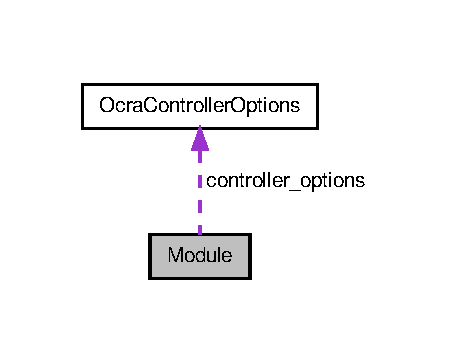
\includegraphics[width=216pt]{classModule__coll__graph}
\end{center}
\end{figure}
\subsection*{\-Public \-Member \-Functions}
\begin{DoxyCompactItemize}
\item 
\hyperlink{classModule_a5a240a8a9ab1813b17bcb810b24ceaea}{\-Module} ()
\item 
\hyperlink{classModule_a7c9d9c096786d127590fdd8aa2b7d681}{$\sim$\-Module} ()
\item 
bool \hyperlink{classModule_a1f18c762538086e1304ea18e00e51abb}{configure} (yarp\-::os\-::\-Resource\-Finder \&rf)
\item 
bool \hyperlink{classModule_ad53295be6c51e834eec92009c2d7bbf3}{interrupt\-Module} ()
\item 
bool \hyperlink{classModule_ab07583e4393148dfe0fd2ae6e7998a4b}{close} ()
\item 
bool \hyperlink{classModule_a1b1c4963512941537cef766217329a8a}{update\-Module} ()
\item 
void \hyperlink{classModule_a861f70d79b8f36dccf5daae182763bd8}{print\-Help} ()
\end{DoxyCompactItemize}
\subsection*{\-Private \-Attributes}
\begin{DoxyCompactItemize}
\item 
std\-::shared\-\_\-ptr$<$ \hyperlink{classThread}{\-Thread} $>$ \hyperlink{classModule_a39346aa2e2a00801e07f4c127ff004ba}{ctrl\-Thread}
\item 
std\-::shared\-\_\-ptr\*
$<$ wbi\-::whole\-Body\-Interface $>$ \hyperlink{classModule_a0d3efedabcef6ec0db88011ccc2e7205}{robot\-Interface}
\item 
yarp\-::os\-::\-Log \hyperlink{classModule_ae029b50069bf4ff53a6f69a5bae824f6}{y\-Log}
\item 
\hyperlink{classOcraControllerOptions}{\-Ocra\-Controller\-Options} \hyperlink{classModule_a04156183c6e15f118595e3637ab5372f}{controller\-\_\-options}
\item 
double \hyperlink{classModule_a1a20dbf0d18e5020ad85d38a0ba22b88}{avg\-Time}
\item 
double \hyperlink{classModule_af66a2dab82208cb2ea25da22fcaaa4a3}{std\-Dev}
\item 
double \hyperlink{classModule_a5baf8260eb8a45ebbb75474f2b277edc}{avg\-Time\-Used}
\item 
double \hyperlink{classModule_a57060f2788b6dc9906e66432e775e5ac}{std\-Dev\-Used}
\item 
double \hyperlink{classModule_a33fee1e7f977b4f27a2e1488480996fb}{danger\-Period\-Loop\-Time}
\end{DoxyCompactItemize}
\subsection*{\-Static \-Private \-Attributes}
\begin{DoxyCompactItemize}
\item 
static const int \hyperlink{classModule_af73cdfdae53c52ea8488d0d8c4f9083f}{\-D\-E\-F\-A\-U\-L\-T\-\_\-\-T\-H\-R\-E\-A\-D\-\_\-\-P\-E\-R\-I\-O\-D} = 10
\end{DoxyCompactItemize}


\subsection{\-Detailed \-Description}
\-The controller module which launches the controller thread. 

\-Basically all this does is parse the command line arguments and look for the various config and task set files. \-It then instantiates a \-W\-B\-I instance (yarp\-W\-B\-I specifically) and a \hyperlink{classThread}{\-Thread} instance. \-It launches these threads and then basically just waits till it gets a kill (ctrl+c) command to close them down. \-Does a little keeping track of time as well. 

\subsection{\-Constructor \& \-Destructor \-Documentation}
\hypertarget{classModule_a5a240a8a9ab1813b17bcb810b24ceaea}{\index{\-Module@{\-Module}!\-Module@{\-Module}}
\index{\-Module@{\-Module}!Module@{\-Module}}
\subsubsection[{\-Module}]{\setlength{\rightskip}{0pt plus 5cm}{\bf \-Module\-::\-Module} (
\begin{DoxyParamCaption}
{}
\end{DoxyParamCaption}
)}}\label{classModule_a5a240a8a9ab1813b17bcb810b24ceaea}
\-Constructor which essentially does nothing. \hypertarget{classModule_a7c9d9c096786d127590fdd8aa2b7d681}{\index{\-Module@{\-Module}!$\sim$\-Module@{$\sim$\-Module}}
\index{$\sim$\-Module@{$\sim$\-Module}!Module@{\-Module}}
\subsubsection[{$\sim$\-Module}]{\setlength{\rightskip}{0pt plus 5cm}{\bf \-Module\-::$\sim$\-Module} (
\begin{DoxyParamCaption}
{}
\end{DoxyParamCaption}
)}}\label{classModule_a7c9d9c096786d127590fdd8aa2b7d681}
\-Destructor which essentially does nothing. 

\subsection{\-Member \-Function \-Documentation}
\hypertarget{classModule_ab07583e4393148dfe0fd2ae6e7998a4b}{\index{\-Module@{\-Module}!close@{close}}
\index{close@{close}!Module@{\-Module}}
\subsubsection[{close}]{\setlength{\rightskip}{0pt plus 5cm}bool {\bf \-Module\-::close} (
\begin{DoxyParamCaption}
{}
\end{DoxyParamCaption}
)}}\label{classModule_ab07583e4393148dfe0fd2ae6e7998a4b}
\-Closes the module. \-First shuts down the threads. \hypertarget{classModule_a1f18c762538086e1304ea18e00e51abb}{\index{\-Module@{\-Module}!configure@{configure}}
\index{configure@{configure}!Module@{\-Module}}
\subsubsection[{configure}]{\setlength{\rightskip}{0pt plus 5cm}bool {\bf \-Module\-::configure} (
\begin{DoxyParamCaption}
\item[{yarp\-::os\-::\-Resource\-Finder \&}]{rf}
\end{DoxyParamCaption}
)}}\label{classModule_a1f18c762538086e1304ea18e00e51abb}
\-Configures the module by parsing the \-R\-F contents. 
\begin{DoxyParams}{\-Parameters}
{\em rf} & \-A resource finder instance which is initialized from the command line args.\\
\hline
\end{DoxyParams}
\begin{DoxyReturn}{\-Returns}
\-True or false if the configuration was successful. 
\end{DoxyReturn}
\hypertarget{classModule_ad53295be6c51e834eec92009c2d7bbf3}{\index{\-Module@{\-Module}!interrupt\-Module@{interrupt\-Module}}
\index{interrupt\-Module@{interrupt\-Module}!Module@{\-Module}}
\subsubsection[{interrupt\-Module}]{\setlength{\rightskip}{0pt plus 5cm}bool {\bf \-Module\-::interrupt\-Module} (
\begin{DoxyParamCaption}
{}
\end{DoxyParamCaption}
)}}\label{classModule_ad53295be6c51e834eec92009c2d7bbf3}
\-Interrupts the module execution and stops the control and wbi threads. \hypertarget{classModule_a861f70d79b8f36dccf5daae182763bd8}{\index{\-Module@{\-Module}!print\-Help@{print\-Help}}
\index{print\-Help@{print\-Help}!Module@{\-Module}}
\subsubsection[{print\-Help}]{\setlength{\rightskip}{0pt plus 5cm}void {\bf \-Module\-::print\-Help} (
\begin{DoxyParamCaption}
{}
\end{DoxyParamCaption}
)}}\label{classModule_a861f70d79b8f36dccf5daae182763bd8}
\-Prints all the command line args one could use. \hypertarget{classModule_a1b1c4963512941537cef766217329a8a}{\index{\-Module@{\-Module}!update\-Module@{update\-Module}}
\index{update\-Module@{update\-Module}!Module@{\-Module}}
\subsubsection[{update\-Module}]{\setlength{\rightskip}{0pt plus 5cm}bool {\bf \-Module\-::update\-Module} (
\begin{DoxyParamCaption}
{}
\end{DoxyParamCaption}
)}}\label{classModule_a1b1c4963512941537cef766217329a8a}
\-Updates the \hyperlink{classModule}{\-Module}. \-Basically just clocks the thread run() method. \begin{DoxyReturn}{\-Returns}
\-Whether or not the clocking functions worked. 
\end{DoxyReturn}


\subsection{\-Member \-Data \-Documentation}
\hypertarget{classModule_a1a20dbf0d18e5020ad85d38a0ba22b88}{\index{\-Module@{\-Module}!avg\-Time@{avg\-Time}}
\index{avg\-Time@{avg\-Time}!Module@{\-Module}}
\subsubsection[{avg\-Time}]{\setlength{\rightskip}{0pt plus 5cm}double {\bf \-Module\-::avg\-Time}\hspace{0.3cm}{\ttfamily  \mbox{[}private\mbox{]}}}}\label{classModule_a1a20dbf0d18e5020ad85d38a0ba22b88}
\-Average time between successive calls of the `run()` method. \hypertarget{classModule_a5baf8260eb8a45ebbb75474f2b277edc}{\index{\-Module@{\-Module}!avg\-Time\-Used@{avg\-Time\-Used}}
\index{avg\-Time\-Used@{avg\-Time\-Used}!Module@{\-Module}}
\subsubsection[{avg\-Time\-Used}]{\setlength{\rightskip}{0pt plus 5cm}double {\bf \-Module\-::avg\-Time\-Used}\hspace{0.3cm}{\ttfamily  \mbox{[}private\mbox{]}}}}\label{classModule_a5baf8260eb8a45ebbb75474f2b277edc}
\-Average time for the `run()` method to execute. \-Should be close to avg\-Time. \hypertarget{classModule_a04156183c6e15f118595e3637ab5372f}{\index{\-Module@{\-Module}!controller\-\_\-options@{controller\-\_\-options}}
\index{controller\-\_\-options@{controller\-\_\-options}!Module@{\-Module}}
\subsubsection[{controller\-\_\-options}]{\setlength{\rightskip}{0pt plus 5cm}{\bf \-Ocra\-Controller\-Options} {\bf \-Module\-::controller\-\_\-options}\hspace{0.3cm}{\ttfamily  \mbox{[}private\mbox{]}}}}\label{classModule_a04156183c6e15f118595e3637ab5372f}
\-Options used for the controller. \hypertarget{classModule_a39346aa2e2a00801e07f4c127ff004ba}{\index{\-Module@{\-Module}!ctrl\-Thread@{ctrl\-Thread}}
\index{ctrl\-Thread@{ctrl\-Thread}!Module@{\-Module}}
\subsubsection[{ctrl\-Thread}]{\setlength{\rightskip}{0pt plus 5cm}std\-::shared\-\_\-ptr$<${\bf \-Thread}$>$ {\bf \-Module\-::ctrl\-Thread}\hspace{0.3cm}{\ttfamily  \mbox{[}private\mbox{]}}}}\label{classModule_a39346aa2e2a00801e07f4c127ff004ba}
\-The controller thread. \-This is where the magic happens. \hypertarget{classModule_a33fee1e7f977b4f27a2e1488480996fb}{\index{\-Module@{\-Module}!danger\-Period\-Loop\-Time@{danger\-Period\-Loop\-Time}}
\index{danger\-Period\-Loop\-Time@{danger\-Period\-Loop\-Time}!Module@{\-Module}}
\subsubsection[{danger\-Period\-Loop\-Time}]{\setlength{\rightskip}{0pt plus 5cm}double {\bf \-Module\-::danger\-Period\-Loop\-Time}\hspace{0.3cm}{\ttfamily  \mbox{[}private\mbox{]}}}}\label{classModule_a33fee1e7f977b4f27a2e1488480996fb}
\-A value which the thread period loop time should not exceed. \hypertarget{classModule_af73cdfdae53c52ea8488d0d8c4f9083f}{\index{\-Module@{\-Module}!\-D\-E\-F\-A\-U\-L\-T\-\_\-\-T\-H\-R\-E\-A\-D\-\_\-\-P\-E\-R\-I\-O\-D@{\-D\-E\-F\-A\-U\-L\-T\-\_\-\-T\-H\-R\-E\-A\-D\-\_\-\-P\-E\-R\-I\-O\-D}}
\index{\-D\-E\-F\-A\-U\-L\-T\-\_\-\-T\-H\-R\-E\-A\-D\-\_\-\-P\-E\-R\-I\-O\-D@{\-D\-E\-F\-A\-U\-L\-T\-\_\-\-T\-H\-R\-E\-A\-D\-\_\-\-P\-E\-R\-I\-O\-D}!Module@{\-Module}}
\subsubsection[{\-D\-E\-F\-A\-U\-L\-T\-\_\-\-T\-H\-R\-E\-A\-D\-\_\-\-P\-E\-R\-I\-O\-D}]{\setlength{\rightskip}{0pt plus 5cm}const int {\bf \-Module\-::\-D\-E\-F\-A\-U\-L\-T\-\_\-\-T\-H\-R\-E\-A\-D\-\_\-\-P\-E\-R\-I\-O\-D} = 10\hspace{0.3cm}{\ttfamily  \mbox{[}static, private\mbox{]}}}}\label{classModule_af73cdfdae53c52ea8488d0d8c4f9083f}
\-If the user doesn't provide a thread period make it 10ms. \hypertarget{classModule_a0d3efedabcef6ec0db88011ccc2e7205}{\index{\-Module@{\-Module}!robot\-Interface@{robot\-Interface}}
\index{robot\-Interface@{robot\-Interface}!Module@{\-Module}}
\subsubsection[{robot\-Interface}]{\setlength{\rightskip}{0pt plus 5cm}std\-::shared\-\_\-ptr$<$wbi\-::whole\-Body\-Interface$>$ {\bf \-Module\-::robot\-Interface}\hspace{0.3cm}{\ttfamily  \mbox{[}private\mbox{]}}}}\label{classModule_a0d3efedabcef6ec0db88011ccc2e7205}
\-The yarp\-W\-B\-I interface used to get estimates from the robot. \hypertarget{classModule_af66a2dab82208cb2ea25da22fcaaa4a3}{\index{\-Module@{\-Module}!std\-Dev@{std\-Dev}}
\index{std\-Dev@{std\-Dev}!Module@{\-Module}}
\subsubsection[{std\-Dev}]{\setlength{\rightskip}{0pt plus 5cm}double {\bf \-Module\-::std\-Dev}\hspace{0.3cm}{\ttfamily  \mbox{[}private\mbox{]}}}}\label{classModule_af66a2dab82208cb2ea25da22fcaaa4a3}
\-Standard deviation of the average time between successive calls of the `run()` method. \hypertarget{classModule_a57060f2788b6dc9906e66432e775e5ac}{\index{\-Module@{\-Module}!std\-Dev\-Used@{std\-Dev\-Used}}
\index{std\-Dev\-Used@{std\-Dev\-Used}!Module@{\-Module}}
\subsubsection[{std\-Dev\-Used}]{\setlength{\rightskip}{0pt plus 5cm}double {\bf \-Module\-::std\-Dev\-Used}\hspace{0.3cm}{\ttfamily  \mbox{[}private\mbox{]}}}}\label{classModule_a57060f2788b6dc9906e66432e775e5ac}
\-Standard deviation of the average time for the `run()` method to execute. \hypertarget{classModule_ae029b50069bf4ff53a6f69a5bae824f6}{\index{\-Module@{\-Module}!y\-Log@{y\-Log}}
\index{y\-Log@{y\-Log}!Module@{\-Module}}
\subsubsection[{y\-Log}]{\setlength{\rightskip}{0pt plus 5cm}yarp\-::os\-::\-Log {\bf \-Module\-::y\-Log}\hspace{0.3cm}{\ttfamily  \mbox{[}private\mbox{]}}}}\label{classModule_ae029b50069bf4ff53a6f69a5bae824f6}
\-A yarp logging tool. 

\-The documentation for this class was generated from the following files\-:\begin{DoxyCompactItemize}
\item 
ocra-\/wbi-\/plugins/ocra-\/icub-\/server/include/ocra-\/icub-\/server/\hyperlink{Module_8h}{\-Module.\-h}\item 
ocra-\/wbi-\/plugins/ocra-\/icub-\/server/src/\hyperlink{Module_8cpp}{\-Module.\-cpp}\end{DoxyCompactItemize}

\hypertarget{classOcraControllerOptions}{\section{\-Ocra\-Controller\-Options \-Class \-Reference}
\label{classOcraControllerOptions}\index{\-Ocra\-Controller\-Options@{\-Ocra\-Controller\-Options}}
}


{\ttfamily \#include $<$\-Thread.\-h$>$}

\subsection*{\-Public \-Member \-Functions}
\begin{DoxyCompactItemize}
\item 
\hyperlink{classOcraControllerOptions_a1a91de992c42c6da488e95cd594eca80}{\-Ocra\-Controller\-Options} ()
\item 
\hyperlink{classOcraControllerOptions_a22f514e92ccf91cc362c48a6c340ac19}{$\sim$\-Ocra\-Controller\-Options} ()
\end{DoxyCompactItemize}
\subsection*{\-Public \-Attributes}
\begin{DoxyCompactItemize}
\item 
int \hyperlink{classOcraControllerOptions_ab706ae593bf5b30433cfd6f957b51db4}{thread\-Period}
\item 
std\-::string \hyperlink{classOcraControllerOptions_a22380b083fbf0b202993d0415d1d4c83}{server\-Name}
\item 
std\-::string \hyperlink{classOcraControllerOptions_a897948011f23b08ba20e1707033458d4}{robot\-Name}
\item 
std\-::string \hyperlink{classOcraControllerOptions_af91566ecff3f7ed02571369c7af061ce}{startup\-Task\-Set\-Path}
\item 
std\-::string \hyperlink{classOcraControllerOptions_ab01efbd786ad8bc5beb6de02dbcd0936}{startup\-Sequence}
\item 
std\-::string \hyperlink{classOcraControllerOptions_af3a98210531cf667c2838e45b470a66e}{wbi\-Config\-File\-Path}
\item 
std\-::string \hyperlink{classOcraControllerOptions_a697196e6267b2a519dd0bcc2bc03ab73}{urdf\-Model\-Path}
\item 
bool \hyperlink{classOcraControllerOptions_a26dce90c0e6cf7ba608020d01cd08f3c}{run\-In\-Debug\-Mode}
\item 
bool \hyperlink{classOcraControllerOptions_af05db2783f36f469fa535fd4ba5c12b1}{no\-Output\-Mode}
\item 
bool \hyperlink{classOcraControllerOptions_a1edf322553d88c1ac2bf8947e9d942d7}{is\-Floating\-Base}
\item 
bool \hyperlink{classOcraControllerOptions_a335f09b446b6d10e2a8e6eb453391d9e}{use\-Odometry}
\item 
bool \hyperlink{classOcraControllerOptions_a34c0a162302f4f2c462d9ce4818292d5}{idle\-Ankles}
\item 
double \hyperlink{classOcraControllerOptions_af09053d38fbafe448a35804ea86d27aa}{idle\-Ankle\-Time}
\item 
bool \hyperlink{classOcraControllerOptions_ae7b16a5b8264abd18ee8761eb1091ccf}{maintain\-Final\-Posture}
\item 
yarp\-::os\-::\-Property \hyperlink{classOcraControllerOptions_ac3965bdcce6cb2ce3e4a335f855acd63}{yarp\-Wbi\-Options}
\item 
ocra\-\_\-recipes\-::\-C\-O\-N\-T\-R\-O\-L\-L\-E\-R\-\_\-\-T\-Y\-P\-E \hyperlink{classOcraControllerOptions_aa533fe11c53b7fb17105f1edf48e1c0d}{controller\-Type}
\item 
ocra\-\_\-recipes\-::\-S\-O\-L\-V\-E\-R\-\_\-\-T\-Y\-P\-E \hyperlink{classOcraControllerOptions_af79b8705c3f3097b642262bc877eaa8e}{solver}
\item 
double \hyperlink{classOcraControllerOptions_aab63ca12dec23284464b978c4e3e1c62}{w\-Ddq}
\item 
double \hyperlink{classOcraControllerOptions_ada37aedbe3639334803637b55c650bc0}{w\-Tau}
\item 
double \hyperlink{classOcraControllerOptions_a96706a52ac56f2598d03e80c9c778ce7}{w\-Fc}
\end{DoxyCompactItemize}


\subsection{\-Constructor \& \-Destructor \-Documentation}
\hypertarget{classOcraControllerOptions_a1a91de992c42c6da488e95cd594eca80}{\index{\-Ocra\-Controller\-Options@{\-Ocra\-Controller\-Options}!\-Ocra\-Controller\-Options@{\-Ocra\-Controller\-Options}}
\index{\-Ocra\-Controller\-Options@{\-Ocra\-Controller\-Options}!OcraControllerOptions@{\-Ocra\-Controller\-Options}}
\subsubsection[{\-Ocra\-Controller\-Options}]{\setlength{\rightskip}{0pt plus 5cm}{\bf \-Ocra\-Controller\-Options\-::\-Ocra\-Controller\-Options} (
\begin{DoxyParamCaption}
{}
\end{DoxyParamCaption}
)}}\label{classOcraControllerOptions_a1a91de992c42c6da488e95cd594eca80}
\-Constructor. \-Initializes all of the possible values. \hypertarget{classOcraControllerOptions_a22f514e92ccf91cc362c48a6c340ac19}{\index{\-Ocra\-Controller\-Options@{\-Ocra\-Controller\-Options}!$\sim$\-Ocra\-Controller\-Options@{$\sim$\-Ocra\-Controller\-Options}}
\index{$\sim$\-Ocra\-Controller\-Options@{$\sim$\-Ocra\-Controller\-Options}!OcraControllerOptions@{\-Ocra\-Controller\-Options}}
\subsubsection[{$\sim$\-Ocra\-Controller\-Options}]{\setlength{\rightskip}{0pt plus 5cm}{\bf \-Ocra\-Controller\-Options\-::$\sim$\-Ocra\-Controller\-Options} (
\begin{DoxyParamCaption}
{}
\end{DoxyParamCaption}
)}}\label{classOcraControllerOptions_a22f514e92ccf91cc362c48a6c340ac19}
\-Destructor. \-Does nothing. 

\subsection{\-Member \-Data \-Documentation}
\hypertarget{classOcraControllerOptions_aa533fe11c53b7fb17105f1edf48e1c0d}{\index{\-Ocra\-Controller\-Options@{\-Ocra\-Controller\-Options}!controller\-Type@{controller\-Type}}
\index{controller\-Type@{controller\-Type}!OcraControllerOptions@{\-Ocra\-Controller\-Options}}
\subsubsection[{controller\-Type}]{\setlength{\rightskip}{0pt plus 5cm}ocra\-\_\-recipes\-::\-C\-O\-N\-T\-R\-O\-L\-L\-E\-R\-\_\-\-T\-Y\-P\-E {\bf \-Ocra\-Controller\-Options\-::controller\-Type}}}\label{classOcraControllerOptions_aa533fe11c53b7fb17105f1edf48e1c0d}
\-The type of \-O\-C\-R\-A controller to use. \hypertarget{classOcraControllerOptions_a34c0a162302f4f2c462d9ce4818292d5}{\index{\-Ocra\-Controller\-Options@{\-Ocra\-Controller\-Options}!idle\-Ankles@{idle\-Ankles}}
\index{idle\-Ankles@{idle\-Ankles}!OcraControllerOptions@{\-Ocra\-Controller\-Options}}
\subsubsection[{idle\-Ankles}]{\setlength{\rightskip}{0pt plus 5cm}bool {\bf \-Ocra\-Controller\-Options\-::idle\-Ankles}}}\label{classOcraControllerOptions_a34c0a162302f4f2c462d9ce4818292d5}
\-A boolean which tells the controller to idle the ankles for a short period and then pass on to normal operation. \-This is to get the feet flush with the ground. \hypertarget{classOcraControllerOptions_af09053d38fbafe448a35804ea86d27aa}{\index{\-Ocra\-Controller\-Options@{\-Ocra\-Controller\-Options}!idle\-Ankle\-Time@{idle\-Ankle\-Time}}
\index{idle\-Ankle\-Time@{idle\-Ankle\-Time}!OcraControllerOptions@{\-Ocra\-Controller\-Options}}
\subsubsection[{idle\-Ankle\-Time}]{\setlength{\rightskip}{0pt plus 5cm}double {\bf \-Ocra\-Controller\-Options\-::idle\-Ankle\-Time}}}\label{classOcraControllerOptions_af09053d38fbafe448a35804ea86d27aa}
\-Number of seconds to idle the ankle. \-By default 1.\-5s. \hypertarget{classOcraControllerOptions_a1edf322553d88c1ac2bf8947e9d942d7}{\index{\-Ocra\-Controller\-Options@{\-Ocra\-Controller\-Options}!is\-Floating\-Base@{is\-Floating\-Base}}
\index{is\-Floating\-Base@{is\-Floating\-Base}!OcraControllerOptions@{\-Ocra\-Controller\-Options}}
\subsubsection[{is\-Floating\-Base}]{\setlength{\rightskip}{0pt plus 5cm}bool {\bf \-Ocra\-Controller\-Options\-::is\-Floating\-Base}}}\label{classOcraControllerOptions_a1edf322553d88c1ac2bf8947e9d942d7}
a boolean which tells the controller whether the robot has a fixed or floating base. \hypertarget{classOcraControllerOptions_ae7b16a5b8264abd18ee8761eb1091ccf}{\index{\-Ocra\-Controller\-Options@{\-Ocra\-Controller\-Options}!maintain\-Final\-Posture@{maintain\-Final\-Posture}}
\index{maintain\-Final\-Posture@{maintain\-Final\-Posture}!OcraControllerOptions@{\-Ocra\-Controller\-Options}}
\subsubsection[{maintain\-Final\-Posture}]{\setlength{\rightskip}{0pt plus 5cm}bool {\bf \-Ocra\-Controller\-Options\-::maintain\-Final\-Posture}}}\label{classOcraControllerOptions_ae7b16a5b8264abd18ee8761eb1091ccf}
\-A boolean which tells the controller to stay in its final posture when the controller is switched to position mode at the end of usage. \hypertarget{classOcraControllerOptions_af05db2783f36f469fa535fd4ba5c12b1}{\index{\-Ocra\-Controller\-Options@{\-Ocra\-Controller\-Options}!no\-Output\-Mode@{no\-Output\-Mode}}
\index{no\-Output\-Mode@{no\-Output\-Mode}!OcraControllerOptions@{\-Ocra\-Controller\-Options}}
\subsubsection[{no\-Output\-Mode}]{\setlength{\rightskip}{0pt plus 5cm}bool {\bf \-Ocra\-Controller\-Options\-::no\-Output\-Mode}}}\label{classOcraControllerOptions_af05db2783f36f469fa535fd4ba5c12b1}
a boolean which runs the controller in a debugging mode but never sends the torques to the robot. \hypertarget{classOcraControllerOptions_a897948011f23b08ba20e1707033458d4}{\index{\-Ocra\-Controller\-Options@{\-Ocra\-Controller\-Options}!robot\-Name@{robot\-Name}}
\index{robot\-Name@{robot\-Name}!OcraControllerOptions@{\-Ocra\-Controller\-Options}}
\subsubsection[{robot\-Name}]{\setlength{\rightskip}{0pt plus 5cm}std\-::string {\bf \-Ocra\-Controller\-Options\-::robot\-Name}}}\label{classOcraControllerOptions_a897948011f23b08ba20e1707033458d4}
a string with the name of the robot. \hypertarget{classOcraControllerOptions_a26dce90c0e6cf7ba608020d01cd08f3c}{\index{\-Ocra\-Controller\-Options@{\-Ocra\-Controller\-Options}!run\-In\-Debug\-Mode@{run\-In\-Debug\-Mode}}
\index{run\-In\-Debug\-Mode@{run\-In\-Debug\-Mode}!OcraControllerOptions@{\-Ocra\-Controller\-Options}}
\subsubsection[{run\-In\-Debug\-Mode}]{\setlength{\rightskip}{0pt plus 5cm}bool {\bf \-Ocra\-Controller\-Options\-::run\-In\-Debug\-Mode}}}\label{classOcraControllerOptions_a26dce90c0e6cf7ba608020d01cd08f3c}
a boolean which runs the controller in a debugging mode which allows one to check the controller ouput joint by joint. \hypertarget{classOcraControllerOptions_a22380b083fbf0b202993d0415d1d4c83}{\index{\-Ocra\-Controller\-Options@{\-Ocra\-Controller\-Options}!server\-Name@{server\-Name}}
\index{server\-Name@{server\-Name}!OcraControllerOptions@{\-Ocra\-Controller\-Options}}
\subsubsection[{server\-Name}]{\setlength{\rightskip}{0pt plus 5cm}std\-::string {\bf \-Ocra\-Controller\-Options\-::server\-Name}}}\label{classOcraControllerOptions_a22380b083fbf0b202993d0415d1d4c83}
a string with the name of the controller server. \hypertarget{classOcraControllerOptions_af79b8705c3f3097b642262bc877eaa8e}{\index{\-Ocra\-Controller\-Options@{\-Ocra\-Controller\-Options}!solver@{solver}}
\index{solver@{solver}!OcraControllerOptions@{\-Ocra\-Controller\-Options}}
\subsubsection[{solver}]{\setlength{\rightskip}{0pt plus 5cm}ocra\-\_\-recipes\-::\-S\-O\-L\-V\-E\-R\-\_\-\-T\-Y\-P\-E {\bf \-Ocra\-Controller\-Options\-::solver}}}\label{classOcraControllerOptions_af79b8705c3f3097b642262bc877eaa8e}
\-The type of \-O\-C\-R\-A controller to use. \hypertarget{classOcraControllerOptions_ab01efbd786ad8bc5beb6de02dbcd0936}{\index{\-Ocra\-Controller\-Options@{\-Ocra\-Controller\-Options}!startup\-Sequence@{startup\-Sequence}}
\index{startup\-Sequence@{startup\-Sequence}!OcraControllerOptions@{\-Ocra\-Controller\-Options}}
\subsubsection[{startup\-Sequence}]{\setlength{\rightskip}{0pt plus 5cm}std\-::string {\bf \-Ocra\-Controller\-Options\-::startup\-Sequence}}}\label{classOcraControllerOptions_ab01efbd786ad8bc5beb6de02dbcd0936}
a string with the name of a sequence to run $\ast$$\ast$(will be removed)$\ast$$\ast$. \hypertarget{classOcraControllerOptions_af91566ecff3f7ed02571369c7af061ce}{\index{\-Ocra\-Controller\-Options@{\-Ocra\-Controller\-Options}!startup\-Task\-Set\-Path@{startup\-Task\-Set\-Path}}
\index{startup\-Task\-Set\-Path@{startup\-Task\-Set\-Path}!OcraControllerOptions@{\-Ocra\-Controller\-Options}}
\subsubsection[{startup\-Task\-Set\-Path}]{\setlength{\rightskip}{0pt plus 5cm}std\-::string {\bf \-Ocra\-Controller\-Options\-::startup\-Task\-Set\-Path}}}\label{classOcraControllerOptions_af91566ecff3f7ed02571369c7af061ce}
a string with the absolute path to an xml file with a set of tasks. \hypertarget{classOcraControllerOptions_ab706ae593bf5b30433cfd6f957b51db4}{\index{\-Ocra\-Controller\-Options@{\-Ocra\-Controller\-Options}!thread\-Period@{thread\-Period}}
\index{thread\-Period@{thread\-Period}!OcraControllerOptions@{\-Ocra\-Controller\-Options}}
\subsubsection[{thread\-Period}]{\setlength{\rightskip}{0pt plus 5cm}int {\bf \-Ocra\-Controller\-Options\-::thread\-Period}}}\label{classOcraControllerOptions_ab706ae593bf5b30433cfd6f957b51db4}
\-An int representing the looping period of the controller. \hypertarget{classOcraControllerOptions_a697196e6267b2a519dd0bcc2bc03ab73}{\index{\-Ocra\-Controller\-Options@{\-Ocra\-Controller\-Options}!urdf\-Model\-Path@{urdf\-Model\-Path}}
\index{urdf\-Model\-Path@{urdf\-Model\-Path}!OcraControllerOptions@{\-Ocra\-Controller\-Options}}
\subsubsection[{urdf\-Model\-Path}]{\setlength{\rightskip}{0pt plus 5cm}std\-::string {\bf \-Ocra\-Controller\-Options\-::urdf\-Model\-Path}}}\label{classOcraControllerOptions_a697196e6267b2a519dd0bcc2bc03ab73}
\-Absolute path to the urdf model. \-Used for the odometry. \hypertarget{classOcraControllerOptions_a335f09b446b6d10e2a8e6eb453391d9e}{\index{\-Ocra\-Controller\-Options@{\-Ocra\-Controller\-Options}!use\-Odometry@{use\-Odometry}}
\index{use\-Odometry@{use\-Odometry}!OcraControllerOptions@{\-Ocra\-Controller\-Options}}
\subsubsection[{use\-Odometry}]{\setlength{\rightskip}{0pt plus 5cm}bool {\bf \-Ocra\-Controller\-Options\-::use\-Odometry}}}\label{classOcraControllerOptions_a335f09b446b6d10e2a8e6eb453391d9e}
a boolean which tells the controller to start the odometry, meaning that the world reference frame remains attached to the ground \hypertarget{classOcraControllerOptions_af3a98210531cf667c2838e45b470a66e}{\index{\-Ocra\-Controller\-Options@{\-Ocra\-Controller\-Options}!wbi\-Config\-File\-Path@{wbi\-Config\-File\-Path}}
\index{wbi\-Config\-File\-Path@{wbi\-Config\-File\-Path}!OcraControllerOptions@{\-Ocra\-Controller\-Options}}
\subsubsection[{wbi\-Config\-File\-Path}]{\setlength{\rightskip}{0pt plus 5cm}std\-::string {\bf \-Ocra\-Controller\-Options\-::wbi\-Config\-File\-Path}}}\label{classOcraControllerOptions_af3a98210531cf667c2838e45b470a66e}
\-The absolute path to the configuration file used to initialize the yarp\-W\-B\-I. \hypertarget{classOcraControllerOptions_aab63ca12dec23284464b978c4e3e1c62}{\index{\-Ocra\-Controller\-Options@{\-Ocra\-Controller\-Options}!w\-Ddq@{w\-Ddq}}
\index{w\-Ddq@{w\-Ddq}!OcraControllerOptions@{\-Ocra\-Controller\-Options}}
\subsubsection[{w\-Ddq}]{\setlength{\rightskip}{0pt plus 5cm}double {\bf \-Ocra\-Controller\-Options\-::w\-Ddq}}}\label{classOcraControllerOptions_aab63ca12dec23284464b978c4e3e1c62}
\hypertarget{classOcraControllerOptions_a96706a52ac56f2598d03e80c9c778ce7}{\index{\-Ocra\-Controller\-Options@{\-Ocra\-Controller\-Options}!w\-Fc@{w\-Fc}}
\index{w\-Fc@{w\-Fc}!OcraControllerOptions@{\-Ocra\-Controller\-Options}}
\subsubsection[{w\-Fc}]{\setlength{\rightskip}{0pt plus 5cm}double {\bf \-Ocra\-Controller\-Options\-::w\-Fc}}}\label{classOcraControllerOptions_a96706a52ac56f2598d03e80c9c778ce7}
\hypertarget{classOcraControllerOptions_ada37aedbe3639334803637b55c650bc0}{\index{\-Ocra\-Controller\-Options@{\-Ocra\-Controller\-Options}!w\-Tau@{w\-Tau}}
\index{w\-Tau@{w\-Tau}!OcraControllerOptions@{\-Ocra\-Controller\-Options}}
\subsubsection[{w\-Tau}]{\setlength{\rightskip}{0pt plus 5cm}double {\bf \-Ocra\-Controller\-Options\-::w\-Tau}}}\label{classOcraControllerOptions_ada37aedbe3639334803637b55c650bc0}
\hypertarget{classOcraControllerOptions_ac3965bdcce6cb2ce3e4a335f855acd63}{\index{\-Ocra\-Controller\-Options@{\-Ocra\-Controller\-Options}!yarp\-Wbi\-Options@{yarp\-Wbi\-Options}}
\index{yarp\-Wbi\-Options@{yarp\-Wbi\-Options}!OcraControllerOptions@{\-Ocra\-Controller\-Options}}
\subsubsection[{yarp\-Wbi\-Options}]{\setlength{\rightskip}{0pt plus 5cm}yarp\-::os\-::\-Property {\bf \-Ocra\-Controller\-Options\-::yarp\-Wbi\-Options}}}\label{classOcraControllerOptions_ac3965bdcce6cb2ce3e4a335f855acd63}
\-Options for the \-W\-B\-I used to update the model. 

\-The documentation for this class was generated from the following files\-:\begin{DoxyCompactItemize}
\item 
ocra-\/wbi-\/plugins/ocra-\/icub-\/server/include/ocra-\/icub-\/server/\hyperlink{Thread_8h}{\-Thread.\-h}\item 
ocra-\/wbi-\/plugins/ocra-\/icub-\/server/src/\hyperlink{Thread_8cpp}{\-Thread.\-cpp}\end{DoxyCompactItemize}

\hypertarget{classocra__icub_1_1OcraWbiConversions}{\section{ocra\-\_\-icub\-:\-:\-Ocra\-Wbi\-Conversions \-Class \-Reference}
\label{classocra__icub_1_1OcraWbiConversions}\index{ocra\-\_\-icub\-::\-Ocra\-Wbi\-Conversions@{ocra\-\_\-icub\-::\-Ocra\-Wbi\-Conversions}}
}


{\ttfamily \#include $<$\-Ocra\-Wbi\-Conversions.\-h$>$}

\subsection*{\-Static \-Public \-Member \-Functions}
\begin{DoxyCompactItemize}
\item 
static bool \hyperlink{classocra__icub_1_1OcraWbiConversions_af71562a5f3d4f6e649f1cec0a3d9996b}{eigen\-Dispd\-To\-Wbi\-Frame} (const \-Eigen\-::\-Displacementd \&disp, wbi\-::\-Frame \&frame)
\item 
static bool \hyperlink{classocra__icub_1_1OcraWbiConversions_a403627efa183c8ddbbccabf0dcd5bcaf}{wbi\-Frame\-To\-Eigen\-Dispd} (const wbi\-::\-Frame \&frame, \-Eigen\-::\-Displacementd \&disp)
\item 
static bool \hyperlink{classocra__icub_1_1OcraWbiConversions_a37c2aea3bf156928cb90a16655c24cc9}{wbi\-To\-Ocra\-Twist\-Vector} (\-Eigen\-::\-Twistd \&t\-\_\-wbi, \-Eigen\-::\-Twistd \&t\-\_\-ocra)
\item 
static bool \hyperlink{classocra__icub_1_1OcraWbiConversions_a7725aea95eb71c805def4a064a2693fa}{ocra\-To\-Wbi\-Twist\-Vector} (\-Eigen\-::\-Twistd \&t\-\_\-ocra, \-Eigen\-::\-Twistd \&t\-\_\-wbi)
\item 
static bool \hyperlink{classocra__icub_1_1OcraWbiConversions_a25a64172ebb14db9ddf301880a433964}{wbi\-To\-Ocra\-Seg\-Jacobian} (const \-Eigen\-::\-Matrix\-Xd \&jac, \-Eigen\-::\-Matrix\-Xd \&\-J)
\item 
static bool \hyperlink{classocra__icub_1_1OcraWbiConversions_a86458de950caa3bde3aa1d1aff448be1}{wbi\-To\-Ocra\-Co\-M\-Jacobian} (const \-Eigen\-::\-Matrix\-Xd \&jac, \-Eigen\-::\-Matrix$<$ double, 3, \-Eigen\-::\-Dynamic $>$ \&\-J)
\item 
static bool \hyperlink{classocra__icub_1_1OcraWbiConversions_ac03ed9581c49479b3ade94d58a3295b4}{eigen\-Row\-Major\-To\-Col\-Major} (const \hyperlink{namespaceocra__icub_aa5e36a19ed031c28ca83c207bd7dd83f}{\-Matrix\-Xd\-Rm} \&\-M\-\_\-rm, \-Eigen\-::\-Matrix\-Xd \&\-M)
\item 
static bool \hyperlink{classocra__icub_1_1OcraWbiConversions_abaa2b7a9069b60cfb36cb21e89b98177}{wbi\-To\-Ocra\-Mass\-Matrix} (int qdof, const \-Eigen\-::\-Matrix\-Xd \&\-M\-\_\-wbi, \-Eigen\-::\-Matrix\-Xd \&\-M\-\_\-ocra)
\item 
static bool \hyperlink{classocra__icub_1_1OcraWbiConversions_ae8839dfdc97e2239f4ed8a257d32fb21}{wbi\-To\-Ocra\-Body\-Vector} (int qdof, const \-Eigen\-::\-Vector\-Xd \&v\-\_\-wbi, \-Eigen\-::\-Vector\-Xd \&v\-\_\-ocra)
\item 
static bool \hyperlink{classocra__icub_1_1OcraWbiConversions_a1197be5b35329fbec85de8ee3c4abbd5}{eigen\-To\-Yarp\-Vector} (const \-Eigen\-::\-Vector\-Xd \&eigen\-Vector, yarp\-::sig\-::\-Vector \&yarp\-Vector)
\end{DoxyCompactItemize}
\subsection*{\-Static \-Public \-Attributes}
\begin{DoxyCompactItemize}
\item 
static const int \hyperlink{classocra__icub_1_1OcraWbiConversions_a7c628bd1208c5e70be458d4dffda4d06}{\-D\-I\-M\-\_\-\-T\-R\-A\-N\-S\-L\-A\-T\-I\-O\-N} = 3
\item 
static const int \hyperlink{classocra__icub_1_1OcraWbiConversions_a05e66392df58e9dda2d4db590bdd65a0}{\-D\-I\-M\-\_\-\-R\-O\-T\-A\-T\-I\-O\-N} = 3
\end{DoxyCompactItemize}


\subsection{\-Member \-Function \-Documentation}
\hypertarget{classocra__icub_1_1OcraWbiConversions_af71562a5f3d4f6e649f1cec0a3d9996b}{\index{ocra\-\_\-icub\-::\-Ocra\-Wbi\-Conversions@{ocra\-\_\-icub\-::\-Ocra\-Wbi\-Conversions}!eigen\-Dispd\-To\-Wbi\-Frame@{eigen\-Dispd\-To\-Wbi\-Frame}}
\index{eigen\-Dispd\-To\-Wbi\-Frame@{eigen\-Dispd\-To\-Wbi\-Frame}!ocra_icub::OcraWbiConversions@{ocra\-\_\-icub\-::\-Ocra\-Wbi\-Conversions}}
\subsubsection[{eigen\-Dispd\-To\-Wbi\-Frame}]{\setlength{\rightskip}{0pt plus 5cm}bool {\bf \-Ocra\-Wbi\-Conversions\-::eigen\-Dispd\-To\-Wbi\-Frame} (
\begin{DoxyParamCaption}
\item[{const \-Eigen\-::\-Displacementd \&}]{disp, }
\item[{wbi\-::\-Frame \&}]{frame}
\end{DoxyParamCaption}
)\hspace{0.3cm}{\ttfamily  \mbox{[}static\mbox{]}}}}\label{classocra__icub_1_1OcraWbiConversions_af71562a5f3d4f6e649f1cec0a3d9996b}
\hypertarget{classocra__icub_1_1OcraWbiConversions_ac03ed9581c49479b3ade94d58a3295b4}{\index{ocra\-\_\-icub\-::\-Ocra\-Wbi\-Conversions@{ocra\-\_\-icub\-::\-Ocra\-Wbi\-Conversions}!eigen\-Row\-Major\-To\-Col\-Major@{eigen\-Row\-Major\-To\-Col\-Major}}
\index{eigen\-Row\-Major\-To\-Col\-Major@{eigen\-Row\-Major\-To\-Col\-Major}!ocra_icub::OcraWbiConversions@{ocra\-\_\-icub\-::\-Ocra\-Wbi\-Conversions}}
\subsubsection[{eigen\-Row\-Major\-To\-Col\-Major}]{\setlength{\rightskip}{0pt plus 5cm}bool {\bf \-Ocra\-Wbi\-Conversions\-::eigen\-Row\-Major\-To\-Col\-Major} (
\begin{DoxyParamCaption}
\item[{const {\bf \-Matrix\-Xd\-Rm} \&}]{\-M\-\_\-rm, }
\item[{\-Eigen\-::\-Matrix\-Xd \&}]{\-M}
\end{DoxyParamCaption}
)\hspace{0.3cm}{\ttfamily  \mbox{[}static\mbox{]}}}}\label{classocra__icub_1_1OcraWbiConversions_ac03ed9581c49479b3ade94d58a3295b4}
\hypertarget{classocra__icub_1_1OcraWbiConversions_a1197be5b35329fbec85de8ee3c4abbd5}{\index{ocra\-\_\-icub\-::\-Ocra\-Wbi\-Conversions@{ocra\-\_\-icub\-::\-Ocra\-Wbi\-Conversions}!eigen\-To\-Yarp\-Vector@{eigen\-To\-Yarp\-Vector}}
\index{eigen\-To\-Yarp\-Vector@{eigen\-To\-Yarp\-Vector}!ocra_icub::OcraWbiConversions@{ocra\-\_\-icub\-::\-Ocra\-Wbi\-Conversions}}
\subsubsection[{eigen\-To\-Yarp\-Vector}]{\setlength{\rightskip}{0pt plus 5cm}bool {\bf \-Ocra\-Wbi\-Conversions\-::eigen\-To\-Yarp\-Vector} (
\begin{DoxyParamCaption}
\item[{const \-Eigen\-::\-Vector\-Xd \&}]{eigen\-Vector, }
\item[{yarp\-::sig\-::\-Vector \&}]{yarp\-Vector}
\end{DoxyParamCaption}
)\hspace{0.3cm}{\ttfamily  \mbox{[}static\mbox{]}}}}\label{classocra__icub_1_1OcraWbiConversions_a1197be5b35329fbec85de8ee3c4abbd5}
\hypertarget{classocra__icub_1_1OcraWbiConversions_a7725aea95eb71c805def4a064a2693fa}{\index{ocra\-\_\-icub\-::\-Ocra\-Wbi\-Conversions@{ocra\-\_\-icub\-::\-Ocra\-Wbi\-Conversions}!ocra\-To\-Wbi\-Twist\-Vector@{ocra\-To\-Wbi\-Twist\-Vector}}
\index{ocra\-To\-Wbi\-Twist\-Vector@{ocra\-To\-Wbi\-Twist\-Vector}!ocra_icub::OcraWbiConversions@{ocra\-\_\-icub\-::\-Ocra\-Wbi\-Conversions}}
\subsubsection[{ocra\-To\-Wbi\-Twist\-Vector}]{\setlength{\rightskip}{0pt plus 5cm}bool {\bf \-Ocra\-Wbi\-Conversions\-::ocra\-To\-Wbi\-Twist\-Vector} (
\begin{DoxyParamCaption}
\item[{\-Eigen\-::\-Twistd \&}]{t\-\_\-ocra, }
\item[{\-Eigen\-::\-Twistd \&}]{t\-\_\-wbi}
\end{DoxyParamCaption}
)\hspace{0.3cm}{\ttfamily  \mbox{[}static\mbox{]}}}}\label{classocra__icub_1_1OcraWbiConversions_a7725aea95eb71c805def4a064a2693fa}
\hypertarget{classocra__icub_1_1OcraWbiConversions_a403627efa183c8ddbbccabf0dcd5bcaf}{\index{ocra\-\_\-icub\-::\-Ocra\-Wbi\-Conversions@{ocra\-\_\-icub\-::\-Ocra\-Wbi\-Conversions}!wbi\-Frame\-To\-Eigen\-Dispd@{wbi\-Frame\-To\-Eigen\-Dispd}}
\index{wbi\-Frame\-To\-Eigen\-Dispd@{wbi\-Frame\-To\-Eigen\-Dispd}!ocra_icub::OcraWbiConversions@{ocra\-\_\-icub\-::\-Ocra\-Wbi\-Conversions}}
\subsubsection[{wbi\-Frame\-To\-Eigen\-Dispd}]{\setlength{\rightskip}{0pt plus 5cm}bool {\bf \-Ocra\-Wbi\-Conversions\-::wbi\-Frame\-To\-Eigen\-Dispd} (
\begin{DoxyParamCaption}
\item[{const wbi\-::\-Frame \&}]{frame, }
\item[{\-Eigen\-::\-Displacementd \&}]{disp}
\end{DoxyParamCaption}
)\hspace{0.3cm}{\ttfamily  \mbox{[}static\mbox{]}}}}\label{classocra__icub_1_1OcraWbiConversions_a403627efa183c8ddbbccabf0dcd5bcaf}
\hypertarget{classocra__icub_1_1OcraWbiConversions_ae8839dfdc97e2239f4ed8a257d32fb21}{\index{ocra\-\_\-icub\-::\-Ocra\-Wbi\-Conversions@{ocra\-\_\-icub\-::\-Ocra\-Wbi\-Conversions}!wbi\-To\-Ocra\-Body\-Vector@{wbi\-To\-Ocra\-Body\-Vector}}
\index{wbi\-To\-Ocra\-Body\-Vector@{wbi\-To\-Ocra\-Body\-Vector}!ocra_icub::OcraWbiConversions@{ocra\-\_\-icub\-::\-Ocra\-Wbi\-Conversions}}
\subsubsection[{wbi\-To\-Ocra\-Body\-Vector}]{\setlength{\rightskip}{0pt plus 5cm}bool {\bf \-Ocra\-Wbi\-Conversions\-::wbi\-To\-Ocra\-Body\-Vector} (
\begin{DoxyParamCaption}
\item[{int}]{qdof, }
\item[{const \-Eigen\-::\-Vector\-Xd \&}]{v\-\_\-wbi, }
\item[{\-Eigen\-::\-Vector\-Xd \&}]{v\-\_\-ocra}
\end{DoxyParamCaption}
)\hspace{0.3cm}{\ttfamily  \mbox{[}static\mbox{]}}}}\label{classocra__icub_1_1OcraWbiConversions_ae8839dfdc97e2239f4ed8a257d32fb21}
\hypertarget{classocra__icub_1_1OcraWbiConversions_a86458de950caa3bde3aa1d1aff448be1}{\index{ocra\-\_\-icub\-::\-Ocra\-Wbi\-Conversions@{ocra\-\_\-icub\-::\-Ocra\-Wbi\-Conversions}!wbi\-To\-Ocra\-Co\-M\-Jacobian@{wbi\-To\-Ocra\-Co\-M\-Jacobian}}
\index{wbi\-To\-Ocra\-Co\-M\-Jacobian@{wbi\-To\-Ocra\-Co\-M\-Jacobian}!ocra_icub::OcraWbiConversions@{ocra\-\_\-icub\-::\-Ocra\-Wbi\-Conversions}}
\subsubsection[{wbi\-To\-Ocra\-Co\-M\-Jacobian}]{\setlength{\rightskip}{0pt plus 5cm}bool {\bf \-Ocra\-Wbi\-Conversions\-::wbi\-To\-Ocra\-Co\-M\-Jacobian} (
\begin{DoxyParamCaption}
\item[{const \-Eigen\-::\-Matrix\-Xd \&}]{jac, }
\item[{\-Eigen\-::\-Matrix$<$ double, 3, \-Eigen\-::\-Dynamic $>$ \&}]{\-J}
\end{DoxyParamCaption}
)\hspace{0.3cm}{\ttfamily  \mbox{[}static\mbox{]}}}}\label{classocra__icub_1_1OcraWbiConversions_a86458de950caa3bde3aa1d1aff448be1}
\hypertarget{classocra__icub_1_1OcraWbiConversions_abaa2b7a9069b60cfb36cb21e89b98177}{\index{ocra\-\_\-icub\-::\-Ocra\-Wbi\-Conversions@{ocra\-\_\-icub\-::\-Ocra\-Wbi\-Conversions}!wbi\-To\-Ocra\-Mass\-Matrix@{wbi\-To\-Ocra\-Mass\-Matrix}}
\index{wbi\-To\-Ocra\-Mass\-Matrix@{wbi\-To\-Ocra\-Mass\-Matrix}!ocra_icub::OcraWbiConversions@{ocra\-\_\-icub\-::\-Ocra\-Wbi\-Conversions}}
\subsubsection[{wbi\-To\-Ocra\-Mass\-Matrix}]{\setlength{\rightskip}{0pt plus 5cm}bool {\bf \-Ocra\-Wbi\-Conversions\-::wbi\-To\-Ocra\-Mass\-Matrix} (
\begin{DoxyParamCaption}
\item[{int}]{qdof, }
\item[{const \-Eigen\-::\-Matrix\-Xd \&}]{\-M\-\_\-wbi, }
\item[{\-Eigen\-::\-Matrix\-Xd \&}]{\-M\-\_\-ocra}
\end{DoxyParamCaption}
)\hspace{0.3cm}{\ttfamily  \mbox{[}static\mbox{]}}}}\label{classocra__icub_1_1OcraWbiConversions_abaa2b7a9069b60cfb36cb21e89b98177}
\hypertarget{classocra__icub_1_1OcraWbiConversions_a25a64172ebb14db9ddf301880a433964}{\index{ocra\-\_\-icub\-::\-Ocra\-Wbi\-Conversions@{ocra\-\_\-icub\-::\-Ocra\-Wbi\-Conversions}!wbi\-To\-Ocra\-Seg\-Jacobian@{wbi\-To\-Ocra\-Seg\-Jacobian}}
\index{wbi\-To\-Ocra\-Seg\-Jacobian@{wbi\-To\-Ocra\-Seg\-Jacobian}!ocra_icub::OcraWbiConversions@{ocra\-\_\-icub\-::\-Ocra\-Wbi\-Conversions}}
\subsubsection[{wbi\-To\-Ocra\-Seg\-Jacobian}]{\setlength{\rightskip}{0pt plus 5cm}bool {\bf \-Ocra\-Wbi\-Conversions\-::wbi\-To\-Ocra\-Seg\-Jacobian} (
\begin{DoxyParamCaption}
\item[{const \-Eigen\-::\-Matrix\-Xd \&}]{jac, }
\item[{\-Eigen\-::\-Matrix\-Xd \&}]{\-J}
\end{DoxyParamCaption}
)\hspace{0.3cm}{\ttfamily  \mbox{[}static\mbox{]}}}}\label{classocra__icub_1_1OcraWbiConversions_a25a64172ebb14db9ddf301880a433964}
\hypertarget{classocra__icub_1_1OcraWbiConversions_a37c2aea3bf156928cb90a16655c24cc9}{\index{ocra\-\_\-icub\-::\-Ocra\-Wbi\-Conversions@{ocra\-\_\-icub\-::\-Ocra\-Wbi\-Conversions}!wbi\-To\-Ocra\-Twist\-Vector@{wbi\-To\-Ocra\-Twist\-Vector}}
\index{wbi\-To\-Ocra\-Twist\-Vector@{wbi\-To\-Ocra\-Twist\-Vector}!ocra_icub::OcraWbiConversions@{ocra\-\_\-icub\-::\-Ocra\-Wbi\-Conversions}}
\subsubsection[{wbi\-To\-Ocra\-Twist\-Vector}]{\setlength{\rightskip}{0pt plus 5cm}bool {\bf \-Ocra\-Wbi\-Conversions\-::wbi\-To\-Ocra\-Twist\-Vector} (
\begin{DoxyParamCaption}
\item[{\-Eigen\-::\-Twistd \&}]{t\-\_\-wbi, }
\item[{\-Eigen\-::\-Twistd \&}]{t\-\_\-ocra}
\end{DoxyParamCaption}
)\hspace{0.3cm}{\ttfamily  \mbox{[}static\mbox{]}}}}\label{classocra__icub_1_1OcraWbiConversions_a37c2aea3bf156928cb90a16655c24cc9}


\subsection{\-Member \-Data \-Documentation}
\hypertarget{classocra__icub_1_1OcraWbiConversions_a05e66392df58e9dda2d4db590bdd65a0}{\index{ocra\-\_\-icub\-::\-Ocra\-Wbi\-Conversions@{ocra\-\_\-icub\-::\-Ocra\-Wbi\-Conversions}!\-D\-I\-M\-\_\-\-R\-O\-T\-A\-T\-I\-O\-N@{\-D\-I\-M\-\_\-\-R\-O\-T\-A\-T\-I\-O\-N}}
\index{\-D\-I\-M\-\_\-\-R\-O\-T\-A\-T\-I\-O\-N@{\-D\-I\-M\-\_\-\-R\-O\-T\-A\-T\-I\-O\-N}!ocra_icub::OcraWbiConversions@{ocra\-\_\-icub\-::\-Ocra\-Wbi\-Conversions}}
\subsubsection[{\-D\-I\-M\-\_\-\-R\-O\-T\-A\-T\-I\-O\-N}]{\setlength{\rightskip}{0pt plus 5cm}const int {\bf ocra\-\_\-icub\-::\-Ocra\-Wbi\-Conversions\-::\-D\-I\-M\-\_\-\-R\-O\-T\-A\-T\-I\-O\-N} = 3\hspace{0.3cm}{\ttfamily  \mbox{[}static\mbox{]}}}}\label{classocra__icub_1_1OcraWbiConversions_a05e66392df58e9dda2d4db590bdd65a0}
\hypertarget{classocra__icub_1_1OcraWbiConversions_a7c628bd1208c5e70be458d4dffda4d06}{\index{ocra\-\_\-icub\-::\-Ocra\-Wbi\-Conversions@{ocra\-\_\-icub\-::\-Ocra\-Wbi\-Conversions}!\-D\-I\-M\-\_\-\-T\-R\-A\-N\-S\-L\-A\-T\-I\-O\-N@{\-D\-I\-M\-\_\-\-T\-R\-A\-N\-S\-L\-A\-T\-I\-O\-N}}
\index{\-D\-I\-M\-\_\-\-T\-R\-A\-N\-S\-L\-A\-T\-I\-O\-N@{\-D\-I\-M\-\_\-\-T\-R\-A\-N\-S\-L\-A\-T\-I\-O\-N}!ocra_icub::OcraWbiConversions@{ocra\-\_\-icub\-::\-Ocra\-Wbi\-Conversions}}
\subsubsection[{\-D\-I\-M\-\_\-\-T\-R\-A\-N\-S\-L\-A\-T\-I\-O\-N}]{\setlength{\rightskip}{0pt plus 5cm}const int {\bf ocra\-\_\-icub\-::\-Ocra\-Wbi\-Conversions\-::\-D\-I\-M\-\_\-\-T\-R\-A\-N\-S\-L\-A\-T\-I\-O\-N} = 3\hspace{0.3cm}{\ttfamily  \mbox{[}static\mbox{]}}}}\label{classocra__icub_1_1OcraWbiConversions_a7c628bd1208c5e70be458d4dffda4d06}


\-The documentation for this class was generated from the following files\-:\begin{DoxyCompactItemize}
\item 
ocra-\/wbi-\/plugins/ocra-\/icub/include/ocra-\/icub/\hyperlink{OcraWbiConversions_8h}{\-Ocra\-Wbi\-Conversions.\-h}\item 
ocra-\/wbi-\/plugins/ocra-\/icub/src/\hyperlink{OcraWbiConversions_8cpp}{\-Ocra\-Wbi\-Conversions.\-cpp}\end{DoxyCompactItemize}

\hypertarget{classocra__icub_1_1OcraWbiModel}{\section{ocra\-\_\-icub\-:\-:\-Ocra\-Wbi\-Model \-Class \-Reference}
\label{classocra__icub_1_1OcraWbiModel}\index{ocra\-\_\-icub\-::\-Ocra\-Wbi\-Model@{ocra\-\_\-icub\-::\-Ocra\-Wbi\-Model}}
}


{\ttfamily \#include $<$\-Ocra\-Wbi\-Model.\-h$>$}

\subsection*{\-Classes}
\begin{DoxyCompactItemize}
\item 
struct \hyperlink{structOcraWbiModel_1_1OcraWbiModel__pimpl}{\-Ocra\-Wbi\-Model\-\_\-pimpl}
\end{DoxyCompactItemize}
\subsection*{\-Public \-Member \-Functions}
\begin{DoxyCompactItemize}
\item 
\hyperlink{classocra__icub_1_1OcraWbiModel_a57a4f0f140f56d7ec0a00b31e16f9673}{\-Ocra\-Wbi\-Model} (const std\-::string \&robot\-Name, const int robot\-Num\-D\-O\-F, std\-::shared\-\_\-ptr$<$ wbi\-::whole\-Body\-Interface $>$ wbi, const bool free\-Root)
\item 
virtual \hyperlink{classocra__icub_1_1OcraWbiModel_ade110b2e003ccd49d2baa4f56a954e4b}{$\sim$\-Ocra\-Wbi\-Model} ()
\item 
virtual int \hyperlink{classocra__icub_1_1OcraWbiModel_adf952842e3c031a5000ee37c51fe9b77}{nb\-Segments} () const 
\item 
virtual const \-Eigen\-::\-Vector\-Xd \& \hyperlink{classocra__icub_1_1OcraWbiModel_aecb11984be8a80c66b45d37f5fb992ce}{get\-Actuated\-Dofs} () const 
\item 
virtual const \-Eigen\-::\-Vector\-Xd \& \hyperlink{classocra__icub_1_1OcraWbiModel_a7eeb8088b632036c56841cee96aef7ff}{get\-Joint\-Lower\-Limits} () const 
\item 
virtual const \-Eigen\-::\-Vector\-Xd \& \hyperlink{classocra__icub_1_1OcraWbiModel_aa9303621ea64de2378780e2f5e6618b6}{get\-Joint\-Upper\-Limits} () const 
\item 
virtual const \-Eigen\-::\-Vector\-Xd \& \hyperlink{classocra__icub_1_1OcraWbiModel_adeacb1988bd5a4edfde5ec30caae2df3}{get\-Joint\-Positions} () const 
\item 
virtual const \-Eigen\-::\-Vector\-Xd \& \hyperlink{classocra__icub_1_1OcraWbiModel_a403d66cbc41b7cc5e1323c49d578e447}{get\-Joint\-Velocities} () const 
\item 
virtual const \-Eigen\-::\-Vector\-Xd \& \hyperlink{classocra__icub_1_1OcraWbiModel_a639baccfdc1ca6409e14a4839e0394fe}{get\-Joint\-Torques} () const 
\item 
virtual const \*
\-Eigen\-::\-Displacementd \& \hyperlink{classocra__icub_1_1OcraWbiModel_a3e9c4db6d1ee56984fea44cdd592a1ac}{get\-Free\-Flyer\-Position} () const 
\item 
virtual const \-Eigen\-::\-Twistd \& \hyperlink{classocra__icub_1_1OcraWbiModel_a9fbfa4c9da43f0b1957f25d8ecb792d9}{get\-Free\-Flyer\-Velocity} () const 
\item 
virtual const std\-::string \& \hyperlink{classocra__icub_1_1OcraWbiModel_a83d6bc29496259e0f23cc085e29aa431}{get\-Joint\-Name} (int index) const 
\item 
virtual const int \hyperlink{classocra__icub_1_1OcraWbiModel_a1d0f2eb31988a8c91b11a3343392fcf9}{get\-Segment\-Index} (std\-::string segment\-Name) const 
\item 
virtual const \-Eigen\-::\-Matrix\-Xd \& \hyperlink{classocra__icub_1_1OcraWbiModel_a49df5e4d811b660c72b35b6d822bb529}{get\-Inertia\-Matrix} () const 
\item 
virtual const \-Eigen\-::\-Matrix\-Xd \& \hyperlink{classocra__icub_1_1OcraWbiModel_a2dfc6cc2f527cc3aec668607b36e5fe9}{get\-Inertia\-Matrix\-Inverse} () const 
\item 
virtual const \-Eigen\-::\-Matrix\-Xd \& \hyperlink{classocra__icub_1_1OcraWbiModel_ae8bc8fbe99ae23b45a40ec867ca066f9}{get\-Damping\-Matrix} () const 
\item 
virtual const \-Eigen\-::\-Vector\-Xd \& \hyperlink{classocra__icub_1_1OcraWbiModel_a8cf1d870edf8c069cb1b196e0cab1f67}{get\-Non\-Linear\-Terms} () const 
\item 
virtual const \-Eigen\-::\-Vector\-Xd \& \hyperlink{classocra__icub_1_1OcraWbiModel_aa85e588223e6c40dabb740089b2cf3ea}{get\-Linear\-Terms} () const 
\item 
virtual const \-Eigen\-::\-Vector\-Xd \& \hyperlink{classocra__icub_1_1OcraWbiModel_a57742157dce7e3526a388be7d11321d3}{get\-Gravity\-Terms} () const 
\item 
virtual double \hyperlink{classocra__icub_1_1OcraWbiModel_a7f52d830940df32916f46b905d985505}{get\-Mass} () const 
\item 
virtual const \-Eigen\-::\-Vector3d \& \hyperlink{classocra__icub_1_1OcraWbiModel_a3af6973d940c01a80085d65841bb27a8}{get\-Co\-M\-Position} () const 
\item 
virtual const \-Eigen\-::\-Vector3d \& \hyperlink{classocra__icub_1_1OcraWbiModel_af7f16945aafd4881f1cfd94498a78ebf}{get\-Co\-M\-Velocity} () const 
\item 
virtual const \-Eigen\-::\-Vector3d \& \hyperlink{classocra__icub_1_1OcraWbiModel_a0985fe02b87fa9bcf90439163c622a71}{get\-Co\-M\-Jdot\-Qdot} () const 
\item 
virtual const \-Eigen\-::\-Matrix\*
$<$ double, 3, \-Eigen\-::\-Dynamic $>$ \& \hyperlink{classocra__icub_1_1OcraWbiModel_abc79b9dec9e96e4e8125d26c6be479d6}{get\-Co\-M\-Jacobian} () const 
\item 
virtual const \-Eigen\-::\-Matrix\*
$<$ double, 3, \-Eigen\-::\-Dynamic $>$ \& \hyperlink{classocra__icub_1_1OcraWbiModel_acc2992d42ea92d55e172622c83ec1bdc}{get\-Co\-M\-Jacobian\-Dot} () const 
\item 
virtual const \-Eigen\-::\-Vector3d \& \hyperlink{classocra__icub_1_1OcraWbiModel_a98c163c5f051c36b78ff24810421664c}{get\-Co\-M\-Angular\-Velocity} () const 
\item 
virtual const \-Eigen\-::\-Matrix\*
$<$ double, 3, \-Eigen\-::\-Dynamic $>$ \& \hyperlink{classocra__icub_1_1OcraWbiModel_aede9be679109798e7342351d13ffdfcd}{get\-Co\-M\-Angular\-Jacobian} () const 
\item 
virtual const \*
\-Eigen\-::\-Displacementd \& \hyperlink{classocra__icub_1_1OcraWbiModel_ad6b33c312d04c4bba05e0df67d8bae06}{get\-Segment\-Position} (int index) const 
\item 
virtual const \-Eigen\-::\-Twistd \& \hyperlink{classocra__icub_1_1OcraWbiModel_a273d90e5ad6d3c1e849b996b1cfc1860}{get\-Segment\-Velocity} (int index) const 
\item 
virtual double \hyperlink{classocra__icub_1_1OcraWbiModel_a2d04857d60138f1664b7828e0d3a307d}{get\-Segment\-Mass} (int index) const 
\item 
virtual const \-Eigen\-::\-Vector3d \& \hyperlink{classocra__icub_1_1OcraWbiModel_a2e2dc6611ff436dcd09ba979197e712d}{get\-Segment\-Co\-M} (int index) const 
\item 
virtual const \-Eigen\-::\-Matrix\*
$<$ double, 6, 6 $>$ \& \hyperlink{classocra__icub_1_1OcraWbiModel_af5849bc569b86523cf515a031b5e14a7}{get\-Segment\-Mass\-Matrix} (int index) const 
\item 
virtual const \-Eigen\-::\-Vector3d \& \hyperlink{classocra__icub_1_1OcraWbiModel_a383b0fc03ffb220899aba6b25fcb6272}{get\-Segment\-Moments\-Of\-Inertia} (int index) const 
\item 
virtual const \-Eigen\-::\-Rotation3d \& \hyperlink{classocra__icub_1_1OcraWbiModel_ad9f9d9013433b1bbf5a59914bee38b14}{get\-Segment\-Inertia\-Axes} (int index) const 
\item 
virtual const \-Eigen\-::\-Matrix\*
$<$ double, 6, \-Eigen\-::\-Dynamic $>$ \& \hyperlink{classocra__icub_1_1OcraWbiModel_a5f0aa99b6b6e85b465ad3a5238caeb9d}{get\-Segment\-Jacobian} (int index) const 
\item 
virtual const \-Eigen\-::\-Matrix\*
$<$ double, 6, \-Eigen\-::\-Dynamic $>$ \& \hyperlink{classocra__icub_1_1OcraWbiModel_a5c556d66e590314fa6c44ceb8658d540}{get\-Segment\-Jacobian} (int index, wbi\-::\-Frame \-H\-\_\-world\-\_\-root) const 
\item 
virtual const \-Eigen\-::\-Matrix\*
$<$ double, 6, \-Eigen\-::\-Dynamic $>$ \& \hyperlink{classocra__icub_1_1OcraWbiModel_a0c391aaf9a10840346b35952e89e32fc}{get\-Segment\-Jdot} (int index) const 
\item 
virtual const \-Eigen\-::\-Matrix\*
$<$ double, 6, \-Eigen\-::\-Dynamic $>$ \& \hyperlink{classocra__icub_1_1OcraWbiModel_a4dd0a4cd9f8d710c64e67c0336169321}{get\-Joint\-Jacobian} (int index) const 
\item 
virtual const \-Eigen\-::\-Twistd \& \hyperlink{classocra__icub_1_1OcraWbiModel_a3261757fab0ab980f8b92748bf5d350e}{get\-Segment\-Jdot\-Qdot} (int index) const 
\item 
void \hyperlink{classocra__icub_1_1OcraWbiModel_a309b3554c4eefda46c05b766476f40fb}{print\-All\-Data} ()
\end{DoxyCompactItemize}
\subsection*{\-Protected \-Member \-Functions}
\begin{DoxyCompactItemize}
\item 
virtual void \hyperlink{classocra__icub_1_1OcraWbiModel_a8639b19a514624953e5e58dbde1c8227}{do\-Set\-State} (const \-Eigen\-::\-Vector\-Xd \&q, const \-Eigen\-::\-Vector\-Xd \&q\-\_\-dot)
\item 
virtual void \hyperlink{classocra__icub_1_1OcraWbiModel_a411c844cbde565ed54a224e39a2e65c1}{do\-Set\-State} (const \-Eigen\-::\-Displacementd \&\-H\-\_\-root, const \-Eigen\-::\-Vector\-Xd \&q, const \-Eigen\-::\-Twistd \&\-T\-\_\-root, const \-Eigen\-::\-Vector\-Xd \&q\-\_\-dot)
\item 
virtual void \hyperlink{classocra__icub_1_1OcraWbiModel_a64d40044dff11a6302992d52f1dbde0d}{do\-Set\-Joint\-Positions} (const \-Eigen\-::\-Vector\-Xd \&q)
\item 
virtual void \hyperlink{classocra__icub_1_1OcraWbiModel_a26a758c5ecb02601c066bdfffe5db194}{do\-Set\-Joint\-Velocities} (const \-Eigen\-::\-Vector\-Xd \&dq)
\item 
virtual void \hyperlink{classocra__icub_1_1OcraWbiModel_aa2bb481dc7fdb55c363ac1a404a807e5}{do\-Set\-Free\-Flyer\-Position} (const \-Eigen\-::\-Displacementd \&\-Hroot)
\item 
virtual void \hyperlink{classocra__icub_1_1OcraWbiModel_af740a36f6cc2899dcd6f3507b9703c7f}{do\-Set\-Free\-Flyer\-Velocity} (const \-Eigen\-::\-Twistd \&\-Troot)
\item 
virtual int \hyperlink{classocra__icub_1_1OcraWbiModel_ad6a498c6c66d6145b99e91bc631efb77}{do\-Get\-Segment\-Index} (const std\-::string \&name) const 
\item 
virtual const std\-::string \& \hyperlink{classocra__icub_1_1OcraWbiModel_a6a2231f2baece1608297aa3a256edb79}{do\-Get\-Segment\-Name} (int index) const 
\item 
virtual int \hyperlink{classocra__icub_1_1OcraWbiModel_a88842af1291a413848fc500554b12a36}{do\-Get\-Dof\-Index} (const std\-::string \&name) const 
\item 
virtual const std\-::string \& \hyperlink{classocra__icub_1_1OcraWbiModel_ac4ba9f8c3964d3f043543c8196fee185}{do\-Get\-Dof\-Name} (int index) const 
\item 
virtual const std\-::string \hyperlink{classocra__icub_1_1OcraWbiModel_adfe5a0f1fb82248f8cbf309f88a95e6c}{do\-Segment\-Name} (const std\-::string \&name) const 
\item 
virtual const std\-::string \hyperlink{classocra__icub_1_1OcraWbiModel_a3c6be0fe7bb4f205f9fd6a44bb275fc2}{do\-Dof\-Name} (const std\-::string \&name) const 
\end{DoxyCompactItemize}
\subsection*{\-Private \-Attributes}
\begin{DoxyCompactItemize}
\item 
std\-::shared\-\_\-ptr\*
$<$ wbi\-::whole\-Body\-Interface $>$ \hyperlink{classocra__icub_1_1OcraWbiModel_ae377f000580656227fa9ef69f2f2e71d}{robot}
\item 
boost\-::shared\-\_\-ptr\*
$<$ \hyperlink{structOcraWbiModel_1_1OcraWbiModel__pimpl}{\-Ocra\-Wbi\-Model\-\_\-pimpl} $>$ \hyperlink{classocra__icub_1_1OcraWbiModel_ab649cb769ca4edd345b3c09c43a69bde}{owm\-\_\-pimpl}
\item 
yarp\-::os\-::\-Log \hyperlink{classocra__icub_1_1OcraWbiModel_a047fe9f9a96794af218ea844f09cd402}{y\-Log}
\end{DoxyCompactItemize}


\subsection{\-Constructor \& \-Destructor \-Documentation}
\hypertarget{classocra__icub_1_1OcraWbiModel_a57a4f0f140f56d7ec0a00b31e16f9673}{\index{ocra\-\_\-icub\-::\-Ocra\-Wbi\-Model@{ocra\-\_\-icub\-::\-Ocra\-Wbi\-Model}!\-Ocra\-Wbi\-Model@{\-Ocra\-Wbi\-Model}}
\index{\-Ocra\-Wbi\-Model@{\-Ocra\-Wbi\-Model}!ocra_icub::OcraWbiModel@{ocra\-\_\-icub\-::\-Ocra\-Wbi\-Model}}
\subsubsection[{\-Ocra\-Wbi\-Model}]{\setlength{\rightskip}{0pt plus 5cm}{\bf \-Ocra\-Wbi\-Model\-::\-Ocra\-Wbi\-Model} (
\begin{DoxyParamCaption}
\item[{const std\-::string \&}]{robot\-Name, }
\item[{const int}]{robot\-Num\-D\-O\-F, }
\item[{std\-::shared\-\_\-ptr$<$ wbi\-::whole\-Body\-Interface $>$}]{wbi, }
\item[{const bool}]{free\-Root}
\end{DoxyParamCaption}
)}}\label{classocra__icub_1_1OcraWbiModel_a57a4f0f140f56d7ec0a00b31e16f9673}
\hypertarget{classocra__icub_1_1OcraWbiModel_ade110b2e003ccd49d2baa4f56a954e4b}{\index{ocra\-\_\-icub\-::\-Ocra\-Wbi\-Model@{ocra\-\_\-icub\-::\-Ocra\-Wbi\-Model}!$\sim$\-Ocra\-Wbi\-Model@{$\sim$\-Ocra\-Wbi\-Model}}
\index{$\sim$\-Ocra\-Wbi\-Model@{$\sim$\-Ocra\-Wbi\-Model}!ocra_icub::OcraWbiModel@{ocra\-\_\-icub\-::\-Ocra\-Wbi\-Model}}
\subsubsection[{$\sim$\-Ocra\-Wbi\-Model}]{\setlength{\rightskip}{0pt plus 5cm}{\bf \-Ocra\-Wbi\-Model\-::$\sim$\-Ocra\-Wbi\-Model} (
\begin{DoxyParamCaption}
{}
\end{DoxyParamCaption}
)\hspace{0.3cm}{\ttfamily  \mbox{[}virtual\mbox{]}}}}\label{classocra__icub_1_1OcraWbiModel_ade110b2e003ccd49d2baa4f56a954e4b}


\subsection{\-Member \-Function \-Documentation}
\hypertarget{classocra__icub_1_1OcraWbiModel_a3c6be0fe7bb4f205f9fd6a44bb275fc2}{\index{ocra\-\_\-icub\-::\-Ocra\-Wbi\-Model@{ocra\-\_\-icub\-::\-Ocra\-Wbi\-Model}!do\-Dof\-Name@{do\-Dof\-Name}}
\index{do\-Dof\-Name@{do\-Dof\-Name}!ocra_icub::OcraWbiModel@{ocra\-\_\-icub\-::\-Ocra\-Wbi\-Model}}
\subsubsection[{do\-Dof\-Name}]{\setlength{\rightskip}{0pt plus 5cm}const std\-::string {\bf \-Ocra\-Wbi\-Model\-::do\-Dof\-Name} (
\begin{DoxyParamCaption}
\item[{const std\-::string \&}]{name}
\end{DoxyParamCaption}
) const\hspace{0.3cm}{\ttfamily  \mbox{[}protected, virtual\mbox{]}}}}\label{classocra__icub_1_1OcraWbiModel_a3c6be0fe7bb4f205f9fd6a44bb275fc2}
\hypertarget{classocra__icub_1_1OcraWbiModel_a88842af1291a413848fc500554b12a36}{\index{ocra\-\_\-icub\-::\-Ocra\-Wbi\-Model@{ocra\-\_\-icub\-::\-Ocra\-Wbi\-Model}!do\-Get\-Dof\-Index@{do\-Get\-Dof\-Index}}
\index{do\-Get\-Dof\-Index@{do\-Get\-Dof\-Index}!ocra_icub::OcraWbiModel@{ocra\-\_\-icub\-::\-Ocra\-Wbi\-Model}}
\subsubsection[{do\-Get\-Dof\-Index}]{\setlength{\rightskip}{0pt plus 5cm}int {\bf \-Ocra\-Wbi\-Model\-::do\-Get\-Dof\-Index} (
\begin{DoxyParamCaption}
\item[{const std\-::string \&}]{name}
\end{DoxyParamCaption}
) const\hspace{0.3cm}{\ttfamily  \mbox{[}protected, virtual\mbox{]}}}}\label{classocra__icub_1_1OcraWbiModel_a88842af1291a413848fc500554b12a36}
\hypertarget{classocra__icub_1_1OcraWbiModel_ac4ba9f8c3964d3f043543c8196fee185}{\index{ocra\-\_\-icub\-::\-Ocra\-Wbi\-Model@{ocra\-\_\-icub\-::\-Ocra\-Wbi\-Model}!do\-Get\-Dof\-Name@{do\-Get\-Dof\-Name}}
\index{do\-Get\-Dof\-Name@{do\-Get\-Dof\-Name}!ocra_icub::OcraWbiModel@{ocra\-\_\-icub\-::\-Ocra\-Wbi\-Model}}
\subsubsection[{do\-Get\-Dof\-Name}]{\setlength{\rightskip}{0pt plus 5cm}const std\-::string \& {\bf \-Ocra\-Wbi\-Model\-::do\-Get\-Dof\-Name} (
\begin{DoxyParamCaption}
\item[{int}]{index}
\end{DoxyParamCaption}
) const\hspace{0.3cm}{\ttfamily  \mbox{[}protected, virtual\mbox{]}}}}\label{classocra__icub_1_1OcraWbiModel_ac4ba9f8c3964d3f043543c8196fee185}
\hypertarget{classocra__icub_1_1OcraWbiModel_ad6a498c6c66d6145b99e91bc631efb77}{\index{ocra\-\_\-icub\-::\-Ocra\-Wbi\-Model@{ocra\-\_\-icub\-::\-Ocra\-Wbi\-Model}!do\-Get\-Segment\-Index@{do\-Get\-Segment\-Index}}
\index{do\-Get\-Segment\-Index@{do\-Get\-Segment\-Index}!ocra_icub::OcraWbiModel@{ocra\-\_\-icub\-::\-Ocra\-Wbi\-Model}}
\subsubsection[{do\-Get\-Segment\-Index}]{\setlength{\rightskip}{0pt plus 5cm}int {\bf \-Ocra\-Wbi\-Model\-::do\-Get\-Segment\-Index} (
\begin{DoxyParamCaption}
\item[{const std\-::string \&}]{name}
\end{DoxyParamCaption}
) const\hspace{0.3cm}{\ttfamily  \mbox{[}protected, virtual\mbox{]}}}}\label{classocra__icub_1_1OcraWbiModel_ad6a498c6c66d6145b99e91bc631efb77}
\hypertarget{classocra__icub_1_1OcraWbiModel_a6a2231f2baece1608297aa3a256edb79}{\index{ocra\-\_\-icub\-::\-Ocra\-Wbi\-Model@{ocra\-\_\-icub\-::\-Ocra\-Wbi\-Model}!do\-Get\-Segment\-Name@{do\-Get\-Segment\-Name}}
\index{do\-Get\-Segment\-Name@{do\-Get\-Segment\-Name}!ocra_icub::OcraWbiModel@{ocra\-\_\-icub\-::\-Ocra\-Wbi\-Model}}
\subsubsection[{do\-Get\-Segment\-Name}]{\setlength{\rightskip}{0pt plus 5cm}const std\-::string \& {\bf \-Ocra\-Wbi\-Model\-::do\-Get\-Segment\-Name} (
\begin{DoxyParamCaption}
\item[{int}]{index}
\end{DoxyParamCaption}
) const\hspace{0.3cm}{\ttfamily  \mbox{[}protected, virtual\mbox{]}}}}\label{classocra__icub_1_1OcraWbiModel_a6a2231f2baece1608297aa3a256edb79}
\hypertarget{classocra__icub_1_1OcraWbiModel_adfe5a0f1fb82248f8cbf309f88a95e6c}{\index{ocra\-\_\-icub\-::\-Ocra\-Wbi\-Model@{ocra\-\_\-icub\-::\-Ocra\-Wbi\-Model}!do\-Segment\-Name@{do\-Segment\-Name}}
\index{do\-Segment\-Name@{do\-Segment\-Name}!ocra_icub::OcraWbiModel@{ocra\-\_\-icub\-::\-Ocra\-Wbi\-Model}}
\subsubsection[{do\-Segment\-Name}]{\setlength{\rightskip}{0pt plus 5cm}const std\-::string {\bf \-Ocra\-Wbi\-Model\-::do\-Segment\-Name} (
\begin{DoxyParamCaption}
\item[{const std\-::string \&}]{name}
\end{DoxyParamCaption}
) const\hspace{0.3cm}{\ttfamily  \mbox{[}protected, virtual\mbox{]}}}}\label{classocra__icub_1_1OcraWbiModel_adfe5a0f1fb82248f8cbf309f88a95e6c}
\hypertarget{classocra__icub_1_1OcraWbiModel_aa2bb481dc7fdb55c363ac1a404a807e5}{\index{ocra\-\_\-icub\-::\-Ocra\-Wbi\-Model@{ocra\-\_\-icub\-::\-Ocra\-Wbi\-Model}!do\-Set\-Free\-Flyer\-Position@{do\-Set\-Free\-Flyer\-Position}}
\index{do\-Set\-Free\-Flyer\-Position@{do\-Set\-Free\-Flyer\-Position}!ocra_icub::OcraWbiModel@{ocra\-\_\-icub\-::\-Ocra\-Wbi\-Model}}
\subsubsection[{do\-Set\-Free\-Flyer\-Position}]{\setlength{\rightskip}{0pt plus 5cm}void {\bf \-Ocra\-Wbi\-Model\-::do\-Set\-Free\-Flyer\-Position} (
\begin{DoxyParamCaption}
\item[{const \-Eigen\-::\-Displacementd \&}]{\-Hroot}
\end{DoxyParamCaption}
)\hspace{0.3cm}{\ttfamily  \mbox{[}protected, virtual\mbox{]}}}}\label{classocra__icub_1_1OcraWbiModel_aa2bb481dc7fdb55c363ac1a404a807e5}
\hypertarget{classocra__icub_1_1OcraWbiModel_af740a36f6cc2899dcd6f3507b9703c7f}{\index{ocra\-\_\-icub\-::\-Ocra\-Wbi\-Model@{ocra\-\_\-icub\-::\-Ocra\-Wbi\-Model}!do\-Set\-Free\-Flyer\-Velocity@{do\-Set\-Free\-Flyer\-Velocity}}
\index{do\-Set\-Free\-Flyer\-Velocity@{do\-Set\-Free\-Flyer\-Velocity}!ocra_icub::OcraWbiModel@{ocra\-\_\-icub\-::\-Ocra\-Wbi\-Model}}
\subsubsection[{do\-Set\-Free\-Flyer\-Velocity}]{\setlength{\rightskip}{0pt plus 5cm}void {\bf \-Ocra\-Wbi\-Model\-::do\-Set\-Free\-Flyer\-Velocity} (
\begin{DoxyParamCaption}
\item[{const \-Eigen\-::\-Twistd \&}]{\-Troot}
\end{DoxyParamCaption}
)\hspace{0.3cm}{\ttfamily  \mbox{[}protected, virtual\mbox{]}}}}\label{classocra__icub_1_1OcraWbiModel_af740a36f6cc2899dcd6f3507b9703c7f}
\hypertarget{classocra__icub_1_1OcraWbiModel_a64d40044dff11a6302992d52f1dbde0d}{\index{ocra\-\_\-icub\-::\-Ocra\-Wbi\-Model@{ocra\-\_\-icub\-::\-Ocra\-Wbi\-Model}!do\-Set\-Joint\-Positions@{do\-Set\-Joint\-Positions}}
\index{do\-Set\-Joint\-Positions@{do\-Set\-Joint\-Positions}!ocra_icub::OcraWbiModel@{ocra\-\_\-icub\-::\-Ocra\-Wbi\-Model}}
\subsubsection[{do\-Set\-Joint\-Positions}]{\setlength{\rightskip}{0pt plus 5cm}void {\bf \-Ocra\-Wbi\-Model\-::do\-Set\-Joint\-Positions} (
\begin{DoxyParamCaption}
\item[{const \-Eigen\-::\-Vector\-Xd \&}]{q}
\end{DoxyParamCaption}
)\hspace{0.3cm}{\ttfamily  \mbox{[}protected, virtual\mbox{]}}}}\label{classocra__icub_1_1OcraWbiModel_a64d40044dff11a6302992d52f1dbde0d}
\hypertarget{classocra__icub_1_1OcraWbiModel_a26a758c5ecb02601c066bdfffe5db194}{\index{ocra\-\_\-icub\-::\-Ocra\-Wbi\-Model@{ocra\-\_\-icub\-::\-Ocra\-Wbi\-Model}!do\-Set\-Joint\-Velocities@{do\-Set\-Joint\-Velocities}}
\index{do\-Set\-Joint\-Velocities@{do\-Set\-Joint\-Velocities}!ocra_icub::OcraWbiModel@{ocra\-\_\-icub\-::\-Ocra\-Wbi\-Model}}
\subsubsection[{do\-Set\-Joint\-Velocities}]{\setlength{\rightskip}{0pt plus 5cm}void {\bf \-Ocra\-Wbi\-Model\-::do\-Set\-Joint\-Velocities} (
\begin{DoxyParamCaption}
\item[{const \-Eigen\-::\-Vector\-Xd \&}]{dq}
\end{DoxyParamCaption}
)\hspace{0.3cm}{\ttfamily  \mbox{[}protected, virtual\mbox{]}}}}\label{classocra__icub_1_1OcraWbiModel_a26a758c5ecb02601c066bdfffe5db194}
\hypertarget{classocra__icub_1_1OcraWbiModel_a8639b19a514624953e5e58dbde1c8227}{\index{ocra\-\_\-icub\-::\-Ocra\-Wbi\-Model@{ocra\-\_\-icub\-::\-Ocra\-Wbi\-Model}!do\-Set\-State@{do\-Set\-State}}
\index{do\-Set\-State@{do\-Set\-State}!ocra_icub::OcraWbiModel@{ocra\-\_\-icub\-::\-Ocra\-Wbi\-Model}}
\subsubsection[{do\-Set\-State}]{\setlength{\rightskip}{0pt plus 5cm}void {\bf \-Ocra\-Wbi\-Model\-::do\-Set\-State} (
\begin{DoxyParamCaption}
\item[{const \-Eigen\-::\-Vector\-Xd \&}]{q, }
\item[{const \-Eigen\-::\-Vector\-Xd \&}]{q\-\_\-dot}
\end{DoxyParamCaption}
)\hspace{0.3cm}{\ttfamily  \mbox{[}protected, virtual\mbox{]}}}}\label{classocra__icub_1_1OcraWbiModel_a8639b19a514624953e5e58dbde1c8227}
\hypertarget{classocra__icub_1_1OcraWbiModel_a411c844cbde565ed54a224e39a2e65c1}{\index{ocra\-\_\-icub\-::\-Ocra\-Wbi\-Model@{ocra\-\_\-icub\-::\-Ocra\-Wbi\-Model}!do\-Set\-State@{do\-Set\-State}}
\index{do\-Set\-State@{do\-Set\-State}!ocra_icub::OcraWbiModel@{ocra\-\_\-icub\-::\-Ocra\-Wbi\-Model}}
\subsubsection[{do\-Set\-State}]{\setlength{\rightskip}{0pt plus 5cm}void {\bf \-Ocra\-Wbi\-Model\-::do\-Set\-State} (
\begin{DoxyParamCaption}
\item[{const \-Eigen\-::\-Displacementd \&}]{\-H\-\_\-root, }
\item[{const \-Eigen\-::\-Vector\-Xd \&}]{q, }
\item[{const \-Eigen\-::\-Twistd \&}]{\-T\-\_\-root, }
\item[{const \-Eigen\-::\-Vector\-Xd \&}]{q\-\_\-dot}
\end{DoxyParamCaption}
)\hspace{0.3cm}{\ttfamily  \mbox{[}protected, virtual\mbox{]}}}}\label{classocra__icub_1_1OcraWbiModel_a411c844cbde565ed54a224e39a2e65c1}
\hypertarget{classocra__icub_1_1OcraWbiModel_aecb11984be8a80c66b45d37f5fb992ce}{\index{ocra\-\_\-icub\-::\-Ocra\-Wbi\-Model@{ocra\-\_\-icub\-::\-Ocra\-Wbi\-Model}!get\-Actuated\-Dofs@{get\-Actuated\-Dofs}}
\index{get\-Actuated\-Dofs@{get\-Actuated\-Dofs}!ocra_icub::OcraWbiModel@{ocra\-\_\-icub\-::\-Ocra\-Wbi\-Model}}
\subsubsection[{get\-Actuated\-Dofs}]{\setlength{\rightskip}{0pt plus 5cm}const \-Eigen\-::\-Vector\-Xd \& {\bf \-Ocra\-Wbi\-Model\-::get\-Actuated\-Dofs} (
\begin{DoxyParamCaption}
{}
\end{DoxyParamCaption}
) const\hspace{0.3cm}{\ttfamily  \mbox{[}virtual\mbox{]}}}}\label{classocra__icub_1_1OcraWbiModel_aecb11984be8a80c66b45d37f5fb992ce}
\hypertarget{classocra__icub_1_1OcraWbiModel_aede9be679109798e7342351d13ffdfcd}{\index{ocra\-\_\-icub\-::\-Ocra\-Wbi\-Model@{ocra\-\_\-icub\-::\-Ocra\-Wbi\-Model}!get\-Co\-M\-Angular\-Jacobian@{get\-Co\-M\-Angular\-Jacobian}}
\index{get\-Co\-M\-Angular\-Jacobian@{get\-Co\-M\-Angular\-Jacobian}!ocra_icub::OcraWbiModel@{ocra\-\_\-icub\-::\-Ocra\-Wbi\-Model}}
\subsubsection[{get\-Co\-M\-Angular\-Jacobian}]{\setlength{\rightskip}{0pt plus 5cm}const \-Eigen\-::\-Matrix$<$ double, {\bf \-C\-O\-M\-\_\-\-P\-O\-S\-\_\-\-D\-I\-M}, \-Eigen\-::\-Dynamic $>$ \& {\bf \-Ocra\-Wbi\-Model\-::get\-Co\-M\-Angular\-Jacobian} (
\begin{DoxyParamCaption}
{}
\end{DoxyParamCaption}
) const\hspace{0.3cm}{\ttfamily  \mbox{[}virtual\mbox{]}}}}\label{classocra__icub_1_1OcraWbiModel_aede9be679109798e7342351d13ffdfcd}
\hypertarget{classocra__icub_1_1OcraWbiModel_a98c163c5f051c36b78ff24810421664c}{\index{ocra\-\_\-icub\-::\-Ocra\-Wbi\-Model@{ocra\-\_\-icub\-::\-Ocra\-Wbi\-Model}!get\-Co\-M\-Angular\-Velocity@{get\-Co\-M\-Angular\-Velocity}}
\index{get\-Co\-M\-Angular\-Velocity@{get\-Co\-M\-Angular\-Velocity}!ocra_icub::OcraWbiModel@{ocra\-\_\-icub\-::\-Ocra\-Wbi\-Model}}
\subsubsection[{get\-Co\-M\-Angular\-Velocity}]{\setlength{\rightskip}{0pt plus 5cm}const \-Eigen\-::\-Vector3d \& {\bf \-Ocra\-Wbi\-Model\-::get\-Co\-M\-Angular\-Velocity} (
\begin{DoxyParamCaption}
{}
\end{DoxyParamCaption}
) const\hspace{0.3cm}{\ttfamily  \mbox{[}virtual\mbox{]}}}}\label{classocra__icub_1_1OcraWbiModel_a98c163c5f051c36b78ff24810421664c}
\hypertarget{classocra__icub_1_1OcraWbiModel_abc79b9dec9e96e4e8125d26c6be479d6}{\index{ocra\-\_\-icub\-::\-Ocra\-Wbi\-Model@{ocra\-\_\-icub\-::\-Ocra\-Wbi\-Model}!get\-Co\-M\-Jacobian@{get\-Co\-M\-Jacobian}}
\index{get\-Co\-M\-Jacobian@{get\-Co\-M\-Jacobian}!ocra_icub::OcraWbiModel@{ocra\-\_\-icub\-::\-Ocra\-Wbi\-Model}}
\subsubsection[{get\-Co\-M\-Jacobian}]{\setlength{\rightskip}{0pt plus 5cm}const \-Eigen\-::\-Matrix$<$ double, {\bf \-C\-O\-M\-\_\-\-P\-O\-S\-\_\-\-D\-I\-M}, \-Eigen\-::\-Dynamic $>$ \& {\bf \-Ocra\-Wbi\-Model\-::get\-Co\-M\-Jacobian} (
\begin{DoxyParamCaption}
{}
\end{DoxyParamCaption}
) const\hspace{0.3cm}{\ttfamily  \mbox{[}virtual\mbox{]}}}}\label{classocra__icub_1_1OcraWbiModel_abc79b9dec9e96e4e8125d26c6be479d6}
\hypertarget{classocra__icub_1_1OcraWbiModel_acc2992d42ea92d55e172622c83ec1bdc}{\index{ocra\-\_\-icub\-::\-Ocra\-Wbi\-Model@{ocra\-\_\-icub\-::\-Ocra\-Wbi\-Model}!get\-Co\-M\-Jacobian\-Dot@{get\-Co\-M\-Jacobian\-Dot}}
\index{get\-Co\-M\-Jacobian\-Dot@{get\-Co\-M\-Jacobian\-Dot}!ocra_icub::OcraWbiModel@{ocra\-\_\-icub\-::\-Ocra\-Wbi\-Model}}
\subsubsection[{get\-Co\-M\-Jacobian\-Dot}]{\setlength{\rightskip}{0pt plus 5cm}const \-Eigen\-::\-Matrix$<$ double, {\bf \-C\-O\-M\-\_\-\-P\-O\-S\-\_\-\-D\-I\-M}, \-Eigen\-::\-Dynamic $>$ \& {\bf \-Ocra\-Wbi\-Model\-::get\-Co\-M\-Jacobian\-Dot} (
\begin{DoxyParamCaption}
{}
\end{DoxyParamCaption}
) const\hspace{0.3cm}{\ttfamily  \mbox{[}virtual\mbox{]}}}}\label{classocra__icub_1_1OcraWbiModel_acc2992d42ea92d55e172622c83ec1bdc}
\hypertarget{classocra__icub_1_1OcraWbiModel_a0985fe02b87fa9bcf90439163c622a71}{\index{ocra\-\_\-icub\-::\-Ocra\-Wbi\-Model@{ocra\-\_\-icub\-::\-Ocra\-Wbi\-Model}!get\-Co\-M\-Jdot\-Qdot@{get\-Co\-M\-Jdot\-Qdot}}
\index{get\-Co\-M\-Jdot\-Qdot@{get\-Co\-M\-Jdot\-Qdot}!ocra_icub::OcraWbiModel@{ocra\-\_\-icub\-::\-Ocra\-Wbi\-Model}}
\subsubsection[{get\-Co\-M\-Jdot\-Qdot}]{\setlength{\rightskip}{0pt plus 5cm}const \-Eigen\-::\-Vector3d \& {\bf \-Ocra\-Wbi\-Model\-::get\-Co\-M\-Jdot\-Qdot} (
\begin{DoxyParamCaption}
{}
\end{DoxyParamCaption}
) const\hspace{0.3cm}{\ttfamily  \mbox{[}virtual\mbox{]}}}}\label{classocra__icub_1_1OcraWbiModel_a0985fe02b87fa9bcf90439163c622a71}
\hypertarget{classocra__icub_1_1OcraWbiModel_a3af6973d940c01a80085d65841bb27a8}{\index{ocra\-\_\-icub\-::\-Ocra\-Wbi\-Model@{ocra\-\_\-icub\-::\-Ocra\-Wbi\-Model}!get\-Co\-M\-Position@{get\-Co\-M\-Position}}
\index{get\-Co\-M\-Position@{get\-Co\-M\-Position}!ocra_icub::OcraWbiModel@{ocra\-\_\-icub\-::\-Ocra\-Wbi\-Model}}
\subsubsection[{get\-Co\-M\-Position}]{\setlength{\rightskip}{0pt plus 5cm}const \-Eigen\-::\-Vector3d \& {\bf \-Ocra\-Wbi\-Model\-::get\-Co\-M\-Position} (
\begin{DoxyParamCaption}
{}
\end{DoxyParamCaption}
) const\hspace{0.3cm}{\ttfamily  \mbox{[}virtual\mbox{]}}}}\label{classocra__icub_1_1OcraWbiModel_a3af6973d940c01a80085d65841bb27a8}
\hypertarget{classocra__icub_1_1OcraWbiModel_af7f16945aafd4881f1cfd94498a78ebf}{\index{ocra\-\_\-icub\-::\-Ocra\-Wbi\-Model@{ocra\-\_\-icub\-::\-Ocra\-Wbi\-Model}!get\-Co\-M\-Velocity@{get\-Co\-M\-Velocity}}
\index{get\-Co\-M\-Velocity@{get\-Co\-M\-Velocity}!ocra_icub::OcraWbiModel@{ocra\-\_\-icub\-::\-Ocra\-Wbi\-Model}}
\subsubsection[{get\-Co\-M\-Velocity}]{\setlength{\rightskip}{0pt plus 5cm}const \-Eigen\-::\-Vector3d \& {\bf \-Ocra\-Wbi\-Model\-::get\-Co\-M\-Velocity} (
\begin{DoxyParamCaption}
{}
\end{DoxyParamCaption}
) const\hspace{0.3cm}{\ttfamily  \mbox{[}virtual\mbox{]}}}}\label{classocra__icub_1_1OcraWbiModel_af7f16945aafd4881f1cfd94498a78ebf}
\hypertarget{classocra__icub_1_1OcraWbiModel_ae8bc8fbe99ae23b45a40ec867ca066f9}{\index{ocra\-\_\-icub\-::\-Ocra\-Wbi\-Model@{ocra\-\_\-icub\-::\-Ocra\-Wbi\-Model}!get\-Damping\-Matrix@{get\-Damping\-Matrix}}
\index{get\-Damping\-Matrix@{get\-Damping\-Matrix}!ocra_icub::OcraWbiModel@{ocra\-\_\-icub\-::\-Ocra\-Wbi\-Model}}
\subsubsection[{get\-Damping\-Matrix}]{\setlength{\rightskip}{0pt plus 5cm}const \-Eigen\-::\-Matrix\-Xd \& {\bf \-Ocra\-Wbi\-Model\-::get\-Damping\-Matrix} (
\begin{DoxyParamCaption}
{}
\end{DoxyParamCaption}
) const\hspace{0.3cm}{\ttfamily  \mbox{[}virtual\mbox{]}}}}\label{classocra__icub_1_1OcraWbiModel_ae8bc8fbe99ae23b45a40ec867ca066f9}
\hypertarget{classocra__icub_1_1OcraWbiModel_a3e9c4db6d1ee56984fea44cdd592a1ac}{\index{ocra\-\_\-icub\-::\-Ocra\-Wbi\-Model@{ocra\-\_\-icub\-::\-Ocra\-Wbi\-Model}!get\-Free\-Flyer\-Position@{get\-Free\-Flyer\-Position}}
\index{get\-Free\-Flyer\-Position@{get\-Free\-Flyer\-Position}!ocra_icub::OcraWbiModel@{ocra\-\_\-icub\-::\-Ocra\-Wbi\-Model}}
\subsubsection[{get\-Free\-Flyer\-Position}]{\setlength{\rightskip}{0pt plus 5cm}const \-Eigen\-::\-Displacementd \& {\bf \-Ocra\-Wbi\-Model\-::get\-Free\-Flyer\-Position} (
\begin{DoxyParamCaption}
{}
\end{DoxyParamCaption}
) const\hspace{0.3cm}{\ttfamily  \mbox{[}virtual\mbox{]}}}}\label{classocra__icub_1_1OcraWbiModel_a3e9c4db6d1ee56984fea44cdd592a1ac}
\hypertarget{classocra__icub_1_1OcraWbiModel_a9fbfa4c9da43f0b1957f25d8ecb792d9}{\index{ocra\-\_\-icub\-::\-Ocra\-Wbi\-Model@{ocra\-\_\-icub\-::\-Ocra\-Wbi\-Model}!get\-Free\-Flyer\-Velocity@{get\-Free\-Flyer\-Velocity}}
\index{get\-Free\-Flyer\-Velocity@{get\-Free\-Flyer\-Velocity}!ocra_icub::OcraWbiModel@{ocra\-\_\-icub\-::\-Ocra\-Wbi\-Model}}
\subsubsection[{get\-Free\-Flyer\-Velocity}]{\setlength{\rightskip}{0pt plus 5cm}const \-Eigen\-::\-Twistd \& {\bf \-Ocra\-Wbi\-Model\-::get\-Free\-Flyer\-Velocity} (
\begin{DoxyParamCaption}
{}
\end{DoxyParamCaption}
) const\hspace{0.3cm}{\ttfamily  \mbox{[}virtual\mbox{]}}}}\label{classocra__icub_1_1OcraWbiModel_a9fbfa4c9da43f0b1957f25d8ecb792d9}
\hypertarget{classocra__icub_1_1OcraWbiModel_a57742157dce7e3526a388be7d11321d3}{\index{ocra\-\_\-icub\-::\-Ocra\-Wbi\-Model@{ocra\-\_\-icub\-::\-Ocra\-Wbi\-Model}!get\-Gravity\-Terms@{get\-Gravity\-Terms}}
\index{get\-Gravity\-Terms@{get\-Gravity\-Terms}!ocra_icub::OcraWbiModel@{ocra\-\_\-icub\-::\-Ocra\-Wbi\-Model}}
\subsubsection[{get\-Gravity\-Terms}]{\setlength{\rightskip}{0pt plus 5cm}const \-Eigen\-::\-Vector\-Xd \& {\bf \-Ocra\-Wbi\-Model\-::get\-Gravity\-Terms} (
\begin{DoxyParamCaption}
{}
\end{DoxyParamCaption}
) const\hspace{0.3cm}{\ttfamily  \mbox{[}virtual\mbox{]}}}}\label{classocra__icub_1_1OcraWbiModel_a57742157dce7e3526a388be7d11321d3}
\hypertarget{classocra__icub_1_1OcraWbiModel_a49df5e4d811b660c72b35b6d822bb529}{\index{ocra\-\_\-icub\-::\-Ocra\-Wbi\-Model@{ocra\-\_\-icub\-::\-Ocra\-Wbi\-Model}!get\-Inertia\-Matrix@{get\-Inertia\-Matrix}}
\index{get\-Inertia\-Matrix@{get\-Inertia\-Matrix}!ocra_icub::OcraWbiModel@{ocra\-\_\-icub\-::\-Ocra\-Wbi\-Model}}
\subsubsection[{get\-Inertia\-Matrix}]{\setlength{\rightskip}{0pt plus 5cm}const \-Eigen\-::\-Matrix\-Xd \& {\bf \-Ocra\-Wbi\-Model\-::get\-Inertia\-Matrix} (
\begin{DoxyParamCaption}
{}
\end{DoxyParamCaption}
) const\hspace{0.3cm}{\ttfamily  \mbox{[}virtual\mbox{]}}}}\label{classocra__icub_1_1OcraWbiModel_a49df5e4d811b660c72b35b6d822bb529}
\hypertarget{classocra__icub_1_1OcraWbiModel_a2dfc6cc2f527cc3aec668607b36e5fe9}{\index{ocra\-\_\-icub\-::\-Ocra\-Wbi\-Model@{ocra\-\_\-icub\-::\-Ocra\-Wbi\-Model}!get\-Inertia\-Matrix\-Inverse@{get\-Inertia\-Matrix\-Inverse}}
\index{get\-Inertia\-Matrix\-Inverse@{get\-Inertia\-Matrix\-Inverse}!ocra_icub::OcraWbiModel@{ocra\-\_\-icub\-::\-Ocra\-Wbi\-Model}}
\subsubsection[{get\-Inertia\-Matrix\-Inverse}]{\setlength{\rightskip}{0pt plus 5cm}const \-Eigen\-::\-Matrix\-Xd \& {\bf \-Ocra\-Wbi\-Model\-::get\-Inertia\-Matrix\-Inverse} (
\begin{DoxyParamCaption}
{}
\end{DoxyParamCaption}
) const\hspace{0.3cm}{\ttfamily  \mbox{[}virtual\mbox{]}}}}\label{classocra__icub_1_1OcraWbiModel_a2dfc6cc2f527cc3aec668607b36e5fe9}
\hypertarget{classocra__icub_1_1OcraWbiModel_a4dd0a4cd9f8d710c64e67c0336169321}{\index{ocra\-\_\-icub\-::\-Ocra\-Wbi\-Model@{ocra\-\_\-icub\-::\-Ocra\-Wbi\-Model}!get\-Joint\-Jacobian@{get\-Joint\-Jacobian}}
\index{get\-Joint\-Jacobian@{get\-Joint\-Jacobian}!ocra_icub::OcraWbiModel@{ocra\-\_\-icub\-::\-Ocra\-Wbi\-Model}}
\subsubsection[{get\-Joint\-Jacobian}]{\setlength{\rightskip}{0pt plus 5cm}const \-Eigen\-::\-Matrix$<$ double, 6, \-Eigen\-::\-Dynamic $>$ \& {\bf \-Ocra\-Wbi\-Model\-::get\-Joint\-Jacobian} (
\begin{DoxyParamCaption}
\item[{int}]{index}
\end{DoxyParamCaption}
) const\hspace{0.3cm}{\ttfamily  \mbox{[}virtual\mbox{]}}}}\label{classocra__icub_1_1OcraWbiModel_a4dd0a4cd9f8d710c64e67c0336169321}
\hypertarget{classocra__icub_1_1OcraWbiModel_a7eeb8088b632036c56841cee96aef7ff}{\index{ocra\-\_\-icub\-::\-Ocra\-Wbi\-Model@{ocra\-\_\-icub\-::\-Ocra\-Wbi\-Model}!get\-Joint\-Lower\-Limits@{get\-Joint\-Lower\-Limits}}
\index{get\-Joint\-Lower\-Limits@{get\-Joint\-Lower\-Limits}!ocra_icub::OcraWbiModel@{ocra\-\_\-icub\-::\-Ocra\-Wbi\-Model}}
\subsubsection[{get\-Joint\-Lower\-Limits}]{\setlength{\rightskip}{0pt plus 5cm}const \-Eigen\-::\-Vector\-Xd \& {\bf \-Ocra\-Wbi\-Model\-::get\-Joint\-Lower\-Limits} (
\begin{DoxyParamCaption}
{}
\end{DoxyParamCaption}
) const\hspace{0.3cm}{\ttfamily  \mbox{[}virtual\mbox{]}}}}\label{classocra__icub_1_1OcraWbiModel_a7eeb8088b632036c56841cee96aef7ff}
\hypertarget{classocra__icub_1_1OcraWbiModel_a83d6bc29496259e0f23cc085e29aa431}{\index{ocra\-\_\-icub\-::\-Ocra\-Wbi\-Model@{ocra\-\_\-icub\-::\-Ocra\-Wbi\-Model}!get\-Joint\-Name@{get\-Joint\-Name}}
\index{get\-Joint\-Name@{get\-Joint\-Name}!ocra_icub::OcraWbiModel@{ocra\-\_\-icub\-::\-Ocra\-Wbi\-Model}}
\subsubsection[{get\-Joint\-Name}]{\setlength{\rightskip}{0pt plus 5cm}const std\-::string \& {\bf \-Ocra\-Wbi\-Model\-::get\-Joint\-Name} (
\begin{DoxyParamCaption}
\item[{int}]{index}
\end{DoxyParamCaption}
) const\hspace{0.3cm}{\ttfamily  \mbox{[}virtual\mbox{]}}}}\label{classocra__icub_1_1OcraWbiModel_a83d6bc29496259e0f23cc085e29aa431}
\hypertarget{classocra__icub_1_1OcraWbiModel_adeacb1988bd5a4edfde5ec30caae2df3}{\index{ocra\-\_\-icub\-::\-Ocra\-Wbi\-Model@{ocra\-\_\-icub\-::\-Ocra\-Wbi\-Model}!get\-Joint\-Positions@{get\-Joint\-Positions}}
\index{get\-Joint\-Positions@{get\-Joint\-Positions}!ocra_icub::OcraWbiModel@{ocra\-\_\-icub\-::\-Ocra\-Wbi\-Model}}
\subsubsection[{get\-Joint\-Positions}]{\setlength{\rightskip}{0pt plus 5cm}const \-Eigen\-::\-Vector\-Xd \& {\bf \-Ocra\-Wbi\-Model\-::get\-Joint\-Positions} (
\begin{DoxyParamCaption}
{}
\end{DoxyParamCaption}
) const\hspace{0.3cm}{\ttfamily  \mbox{[}virtual\mbox{]}}}}\label{classocra__icub_1_1OcraWbiModel_adeacb1988bd5a4edfde5ec30caae2df3}
\hypertarget{classocra__icub_1_1OcraWbiModel_a639baccfdc1ca6409e14a4839e0394fe}{\index{ocra\-\_\-icub\-::\-Ocra\-Wbi\-Model@{ocra\-\_\-icub\-::\-Ocra\-Wbi\-Model}!get\-Joint\-Torques@{get\-Joint\-Torques}}
\index{get\-Joint\-Torques@{get\-Joint\-Torques}!ocra_icub::OcraWbiModel@{ocra\-\_\-icub\-::\-Ocra\-Wbi\-Model}}
\subsubsection[{get\-Joint\-Torques}]{\setlength{\rightskip}{0pt plus 5cm}const \-Eigen\-::\-Vector\-Xd \& {\bf \-Ocra\-Wbi\-Model\-::get\-Joint\-Torques} (
\begin{DoxyParamCaption}
{}
\end{DoxyParamCaption}
) const\hspace{0.3cm}{\ttfamily  \mbox{[}virtual\mbox{]}}}}\label{classocra__icub_1_1OcraWbiModel_a639baccfdc1ca6409e14a4839e0394fe}
\hypertarget{classocra__icub_1_1OcraWbiModel_aa9303621ea64de2378780e2f5e6618b6}{\index{ocra\-\_\-icub\-::\-Ocra\-Wbi\-Model@{ocra\-\_\-icub\-::\-Ocra\-Wbi\-Model}!get\-Joint\-Upper\-Limits@{get\-Joint\-Upper\-Limits}}
\index{get\-Joint\-Upper\-Limits@{get\-Joint\-Upper\-Limits}!ocra_icub::OcraWbiModel@{ocra\-\_\-icub\-::\-Ocra\-Wbi\-Model}}
\subsubsection[{get\-Joint\-Upper\-Limits}]{\setlength{\rightskip}{0pt plus 5cm}const \-Eigen\-::\-Vector\-Xd \& {\bf \-Ocra\-Wbi\-Model\-::get\-Joint\-Upper\-Limits} (
\begin{DoxyParamCaption}
{}
\end{DoxyParamCaption}
) const\hspace{0.3cm}{\ttfamily  \mbox{[}virtual\mbox{]}}}}\label{classocra__icub_1_1OcraWbiModel_aa9303621ea64de2378780e2f5e6618b6}
\hypertarget{classocra__icub_1_1OcraWbiModel_a403d66cbc41b7cc5e1323c49d578e447}{\index{ocra\-\_\-icub\-::\-Ocra\-Wbi\-Model@{ocra\-\_\-icub\-::\-Ocra\-Wbi\-Model}!get\-Joint\-Velocities@{get\-Joint\-Velocities}}
\index{get\-Joint\-Velocities@{get\-Joint\-Velocities}!ocra_icub::OcraWbiModel@{ocra\-\_\-icub\-::\-Ocra\-Wbi\-Model}}
\subsubsection[{get\-Joint\-Velocities}]{\setlength{\rightskip}{0pt plus 5cm}const \-Eigen\-::\-Vector\-Xd \& {\bf \-Ocra\-Wbi\-Model\-::get\-Joint\-Velocities} (
\begin{DoxyParamCaption}
{}
\end{DoxyParamCaption}
) const\hspace{0.3cm}{\ttfamily  \mbox{[}virtual\mbox{]}}}}\label{classocra__icub_1_1OcraWbiModel_a403d66cbc41b7cc5e1323c49d578e447}
\hypertarget{classocra__icub_1_1OcraWbiModel_aa85e588223e6c40dabb740089b2cf3ea}{\index{ocra\-\_\-icub\-::\-Ocra\-Wbi\-Model@{ocra\-\_\-icub\-::\-Ocra\-Wbi\-Model}!get\-Linear\-Terms@{get\-Linear\-Terms}}
\index{get\-Linear\-Terms@{get\-Linear\-Terms}!ocra_icub::OcraWbiModel@{ocra\-\_\-icub\-::\-Ocra\-Wbi\-Model}}
\subsubsection[{get\-Linear\-Terms}]{\setlength{\rightskip}{0pt plus 5cm}const \-Eigen\-::\-Vector\-Xd \& {\bf \-Ocra\-Wbi\-Model\-::get\-Linear\-Terms} (
\begin{DoxyParamCaption}
{}
\end{DoxyParamCaption}
) const\hspace{0.3cm}{\ttfamily  \mbox{[}virtual\mbox{]}}}}\label{classocra__icub_1_1OcraWbiModel_aa85e588223e6c40dabb740089b2cf3ea}
\hypertarget{classocra__icub_1_1OcraWbiModel_a7f52d830940df32916f46b905d985505}{\index{ocra\-\_\-icub\-::\-Ocra\-Wbi\-Model@{ocra\-\_\-icub\-::\-Ocra\-Wbi\-Model}!get\-Mass@{get\-Mass}}
\index{get\-Mass@{get\-Mass}!ocra_icub::OcraWbiModel@{ocra\-\_\-icub\-::\-Ocra\-Wbi\-Model}}
\subsubsection[{get\-Mass}]{\setlength{\rightskip}{0pt plus 5cm}double {\bf \-Ocra\-Wbi\-Model\-::get\-Mass} (
\begin{DoxyParamCaption}
{}
\end{DoxyParamCaption}
) const\hspace{0.3cm}{\ttfamily  \mbox{[}virtual\mbox{]}}}}\label{classocra__icub_1_1OcraWbiModel_a7f52d830940df32916f46b905d985505}
\hypertarget{classocra__icub_1_1OcraWbiModel_a8cf1d870edf8c069cb1b196e0cab1f67}{\index{ocra\-\_\-icub\-::\-Ocra\-Wbi\-Model@{ocra\-\_\-icub\-::\-Ocra\-Wbi\-Model}!get\-Non\-Linear\-Terms@{get\-Non\-Linear\-Terms}}
\index{get\-Non\-Linear\-Terms@{get\-Non\-Linear\-Terms}!ocra_icub::OcraWbiModel@{ocra\-\_\-icub\-::\-Ocra\-Wbi\-Model}}
\subsubsection[{get\-Non\-Linear\-Terms}]{\setlength{\rightskip}{0pt plus 5cm}const \-Eigen\-::\-Vector\-Xd \& {\bf \-Ocra\-Wbi\-Model\-::get\-Non\-Linear\-Terms} (
\begin{DoxyParamCaption}
{}
\end{DoxyParamCaption}
) const\hspace{0.3cm}{\ttfamily  \mbox{[}virtual\mbox{]}}}}\label{classocra__icub_1_1OcraWbiModel_a8cf1d870edf8c069cb1b196e0cab1f67}
\hypertarget{classocra__icub_1_1OcraWbiModel_a2e2dc6611ff436dcd09ba979197e712d}{\index{ocra\-\_\-icub\-::\-Ocra\-Wbi\-Model@{ocra\-\_\-icub\-::\-Ocra\-Wbi\-Model}!get\-Segment\-Co\-M@{get\-Segment\-Co\-M}}
\index{get\-Segment\-Co\-M@{get\-Segment\-Co\-M}!ocra_icub::OcraWbiModel@{ocra\-\_\-icub\-::\-Ocra\-Wbi\-Model}}
\subsubsection[{get\-Segment\-Co\-M}]{\setlength{\rightskip}{0pt plus 5cm}const \-Eigen\-::\-Vector3d \& {\bf \-Ocra\-Wbi\-Model\-::get\-Segment\-Co\-M} (
\begin{DoxyParamCaption}
\item[{int}]{index}
\end{DoxyParamCaption}
) const\hspace{0.3cm}{\ttfamily  \mbox{[}virtual\mbox{]}}}}\label{classocra__icub_1_1OcraWbiModel_a2e2dc6611ff436dcd09ba979197e712d}
\hypertarget{classocra__icub_1_1OcraWbiModel_a1d0f2eb31988a8c91b11a3343392fcf9}{\index{ocra\-\_\-icub\-::\-Ocra\-Wbi\-Model@{ocra\-\_\-icub\-::\-Ocra\-Wbi\-Model}!get\-Segment\-Index@{get\-Segment\-Index}}
\index{get\-Segment\-Index@{get\-Segment\-Index}!ocra_icub::OcraWbiModel@{ocra\-\_\-icub\-::\-Ocra\-Wbi\-Model}}
\subsubsection[{get\-Segment\-Index}]{\setlength{\rightskip}{0pt plus 5cm}const int {\bf \-Ocra\-Wbi\-Model\-::get\-Segment\-Index} (
\begin{DoxyParamCaption}
\item[{std\-::string}]{segment\-Name}
\end{DoxyParamCaption}
) const\hspace{0.3cm}{\ttfamily  \mbox{[}virtual\mbox{]}}}}\label{classocra__icub_1_1OcraWbiModel_a1d0f2eb31988a8c91b11a3343392fcf9}
\hypertarget{classocra__icub_1_1OcraWbiModel_ad9f9d9013433b1bbf5a59914bee38b14}{\index{ocra\-\_\-icub\-::\-Ocra\-Wbi\-Model@{ocra\-\_\-icub\-::\-Ocra\-Wbi\-Model}!get\-Segment\-Inertia\-Axes@{get\-Segment\-Inertia\-Axes}}
\index{get\-Segment\-Inertia\-Axes@{get\-Segment\-Inertia\-Axes}!ocra_icub::OcraWbiModel@{ocra\-\_\-icub\-::\-Ocra\-Wbi\-Model}}
\subsubsection[{get\-Segment\-Inertia\-Axes}]{\setlength{\rightskip}{0pt plus 5cm}const \-Eigen\-::\-Rotation3d \& {\bf \-Ocra\-Wbi\-Model\-::get\-Segment\-Inertia\-Axes} (
\begin{DoxyParamCaption}
\item[{int}]{index}
\end{DoxyParamCaption}
) const\hspace{0.3cm}{\ttfamily  \mbox{[}virtual\mbox{]}}}}\label{classocra__icub_1_1OcraWbiModel_ad9f9d9013433b1bbf5a59914bee38b14}
\hypertarget{classocra__icub_1_1OcraWbiModel_a5f0aa99b6b6e85b465ad3a5238caeb9d}{\index{ocra\-\_\-icub\-::\-Ocra\-Wbi\-Model@{ocra\-\_\-icub\-::\-Ocra\-Wbi\-Model}!get\-Segment\-Jacobian@{get\-Segment\-Jacobian}}
\index{get\-Segment\-Jacobian@{get\-Segment\-Jacobian}!ocra_icub::OcraWbiModel@{ocra\-\_\-icub\-::\-Ocra\-Wbi\-Model}}
\subsubsection[{get\-Segment\-Jacobian}]{\setlength{\rightskip}{0pt plus 5cm}const \-Eigen\-::\-Matrix$<$ double, 6, \-Eigen\-::\-Dynamic $>$ \& {\bf \-Ocra\-Wbi\-Model\-::get\-Segment\-Jacobian} (
\begin{DoxyParamCaption}
\item[{int}]{index}
\end{DoxyParamCaption}
) const\hspace{0.3cm}{\ttfamily  \mbox{[}virtual\mbox{]}}}}\label{classocra__icub_1_1OcraWbiModel_a5f0aa99b6b6e85b465ad3a5238caeb9d}
\-We must project the jacobian in the segment frame orientation in order to work with the controller.\hypertarget{classocra__icub_1_1OcraWbiModel_a5c556d66e590314fa6c44ceb8658d540}{\index{ocra\-\_\-icub\-::\-Ocra\-Wbi\-Model@{ocra\-\_\-icub\-::\-Ocra\-Wbi\-Model}!get\-Segment\-Jacobian@{get\-Segment\-Jacobian}}
\index{get\-Segment\-Jacobian@{get\-Segment\-Jacobian}!ocra_icub::OcraWbiModel@{ocra\-\_\-icub\-::\-Ocra\-Wbi\-Model}}
\subsubsection[{get\-Segment\-Jacobian}]{\setlength{\rightskip}{0pt plus 5cm}const \-Eigen\-::\-Matrix$<$ double, 6, \-Eigen\-::\-Dynamic $>$ \& {\bf \-Ocra\-Wbi\-Model\-::get\-Segment\-Jacobian} (
\begin{DoxyParamCaption}
\item[{int}]{index, }
\item[{wbi\-::\-Frame}]{\-H\-\_\-world\-\_\-root}
\end{DoxyParamCaption}
) const\hspace{0.3cm}{\ttfamily  \mbox{[}virtual\mbox{]}}}}\label{classocra__icub_1_1OcraWbiModel_a5c556d66e590314fa6c44ceb8658d540}
\hypertarget{classocra__icub_1_1OcraWbiModel_a0c391aaf9a10840346b35952e89e32fc}{\index{ocra\-\_\-icub\-::\-Ocra\-Wbi\-Model@{ocra\-\_\-icub\-::\-Ocra\-Wbi\-Model}!get\-Segment\-Jdot@{get\-Segment\-Jdot}}
\index{get\-Segment\-Jdot@{get\-Segment\-Jdot}!ocra_icub::OcraWbiModel@{ocra\-\_\-icub\-::\-Ocra\-Wbi\-Model}}
\subsubsection[{get\-Segment\-Jdot}]{\setlength{\rightskip}{0pt plus 5cm}const \-Eigen\-::\-Matrix$<$ double, 6, \-Eigen\-::\-Dynamic $>$ \& {\bf \-Ocra\-Wbi\-Model\-::get\-Segment\-Jdot} (
\begin{DoxyParamCaption}
\item[{int}]{index}
\end{DoxyParamCaption}
) const\hspace{0.3cm}{\ttfamily  \mbox{[}virtual\mbox{]}}}}\label{classocra__icub_1_1OcraWbiModel_a0c391aaf9a10840346b35952e89e32fc}
\hypertarget{classocra__icub_1_1OcraWbiModel_a3261757fab0ab980f8b92748bf5d350e}{\index{ocra\-\_\-icub\-::\-Ocra\-Wbi\-Model@{ocra\-\_\-icub\-::\-Ocra\-Wbi\-Model}!get\-Segment\-Jdot\-Qdot@{get\-Segment\-Jdot\-Qdot}}
\index{get\-Segment\-Jdot\-Qdot@{get\-Segment\-Jdot\-Qdot}!ocra_icub::OcraWbiModel@{ocra\-\_\-icub\-::\-Ocra\-Wbi\-Model}}
\subsubsection[{get\-Segment\-Jdot\-Qdot}]{\setlength{\rightskip}{0pt plus 5cm}const \-Eigen\-::\-Twistd \& {\bf \-Ocra\-Wbi\-Model\-::get\-Segment\-Jdot\-Qdot} (
\begin{DoxyParamCaption}
\item[{int}]{index}
\end{DoxyParamCaption}
) const\hspace{0.3cm}{\ttfamily  \mbox{[}virtual\mbox{]}}}}\label{classocra__icub_1_1OcraWbiModel_a3261757fab0ab980f8b92748bf5d350e}
\hypertarget{classocra__icub_1_1OcraWbiModel_a2d04857d60138f1664b7828e0d3a307d}{\index{ocra\-\_\-icub\-::\-Ocra\-Wbi\-Model@{ocra\-\_\-icub\-::\-Ocra\-Wbi\-Model}!get\-Segment\-Mass@{get\-Segment\-Mass}}
\index{get\-Segment\-Mass@{get\-Segment\-Mass}!ocra_icub::OcraWbiModel@{ocra\-\_\-icub\-::\-Ocra\-Wbi\-Model}}
\subsubsection[{get\-Segment\-Mass}]{\setlength{\rightskip}{0pt plus 5cm}double {\bf \-Ocra\-Wbi\-Model\-::get\-Segment\-Mass} (
\begin{DoxyParamCaption}
\item[{int}]{index}
\end{DoxyParamCaption}
) const\hspace{0.3cm}{\ttfamily  \mbox{[}virtual\mbox{]}}}}\label{classocra__icub_1_1OcraWbiModel_a2d04857d60138f1664b7828e0d3a307d}
\hypertarget{classocra__icub_1_1OcraWbiModel_af5849bc569b86523cf515a031b5e14a7}{\index{ocra\-\_\-icub\-::\-Ocra\-Wbi\-Model@{ocra\-\_\-icub\-::\-Ocra\-Wbi\-Model}!get\-Segment\-Mass\-Matrix@{get\-Segment\-Mass\-Matrix}}
\index{get\-Segment\-Mass\-Matrix@{get\-Segment\-Mass\-Matrix}!ocra_icub::OcraWbiModel@{ocra\-\_\-icub\-::\-Ocra\-Wbi\-Model}}
\subsubsection[{get\-Segment\-Mass\-Matrix}]{\setlength{\rightskip}{0pt plus 5cm}const \-Eigen\-::\-Matrix$<$ double, 6, 6 $>$ \& {\bf \-Ocra\-Wbi\-Model\-::get\-Segment\-Mass\-Matrix} (
\begin{DoxyParamCaption}
\item[{int}]{index}
\end{DoxyParamCaption}
) const\hspace{0.3cm}{\ttfamily  \mbox{[}virtual\mbox{]}}}}\label{classocra__icub_1_1OcraWbiModel_af5849bc569b86523cf515a031b5e14a7}
\hypertarget{classocra__icub_1_1OcraWbiModel_a383b0fc03ffb220899aba6b25fcb6272}{\index{ocra\-\_\-icub\-::\-Ocra\-Wbi\-Model@{ocra\-\_\-icub\-::\-Ocra\-Wbi\-Model}!get\-Segment\-Moments\-Of\-Inertia@{get\-Segment\-Moments\-Of\-Inertia}}
\index{get\-Segment\-Moments\-Of\-Inertia@{get\-Segment\-Moments\-Of\-Inertia}!ocra_icub::OcraWbiModel@{ocra\-\_\-icub\-::\-Ocra\-Wbi\-Model}}
\subsubsection[{get\-Segment\-Moments\-Of\-Inertia}]{\setlength{\rightskip}{0pt plus 5cm}const \-Eigen\-::\-Vector3d \& {\bf \-Ocra\-Wbi\-Model\-::get\-Segment\-Moments\-Of\-Inertia} (
\begin{DoxyParamCaption}
\item[{int}]{index}
\end{DoxyParamCaption}
) const\hspace{0.3cm}{\ttfamily  \mbox{[}virtual\mbox{]}}}}\label{classocra__icub_1_1OcraWbiModel_a383b0fc03ffb220899aba6b25fcb6272}
\hypertarget{classocra__icub_1_1OcraWbiModel_ad6b33c312d04c4bba05e0df67d8bae06}{\index{ocra\-\_\-icub\-::\-Ocra\-Wbi\-Model@{ocra\-\_\-icub\-::\-Ocra\-Wbi\-Model}!get\-Segment\-Position@{get\-Segment\-Position}}
\index{get\-Segment\-Position@{get\-Segment\-Position}!ocra_icub::OcraWbiModel@{ocra\-\_\-icub\-::\-Ocra\-Wbi\-Model}}
\subsubsection[{get\-Segment\-Position}]{\setlength{\rightskip}{0pt plus 5cm}const \-Eigen\-::\-Displacementd \& {\bf \-Ocra\-Wbi\-Model\-::get\-Segment\-Position} (
\begin{DoxyParamCaption}
\item[{int}]{index}
\end{DoxyParamCaption}
) const\hspace{0.3cm}{\ttfamily  \mbox{[}virtual\mbox{]}}}}\label{classocra__icub_1_1OcraWbiModel_ad6b33c312d04c4bba05e0df67d8bae06}
\hypertarget{classocra__icub_1_1OcraWbiModel_a273d90e5ad6d3c1e849b996b1cfc1860}{\index{ocra\-\_\-icub\-::\-Ocra\-Wbi\-Model@{ocra\-\_\-icub\-::\-Ocra\-Wbi\-Model}!get\-Segment\-Velocity@{get\-Segment\-Velocity}}
\index{get\-Segment\-Velocity@{get\-Segment\-Velocity}!ocra_icub::OcraWbiModel@{ocra\-\_\-icub\-::\-Ocra\-Wbi\-Model}}
\subsubsection[{get\-Segment\-Velocity}]{\setlength{\rightskip}{0pt plus 5cm}const \-Eigen\-::\-Twistd \& {\bf \-Ocra\-Wbi\-Model\-::get\-Segment\-Velocity} (
\begin{DoxyParamCaption}
\item[{int}]{index}
\end{DoxyParamCaption}
) const\hspace{0.3cm}{\ttfamily  \mbox{[}virtual\mbox{]}}}}\label{classocra__icub_1_1OcraWbiModel_a273d90e5ad6d3c1e849b996b1cfc1860}
\hypertarget{classocra__icub_1_1OcraWbiModel_adf952842e3c031a5000ee37c51fe9b77}{\index{ocra\-\_\-icub\-::\-Ocra\-Wbi\-Model@{ocra\-\_\-icub\-::\-Ocra\-Wbi\-Model}!nb\-Segments@{nb\-Segments}}
\index{nb\-Segments@{nb\-Segments}!ocra_icub::OcraWbiModel@{ocra\-\_\-icub\-::\-Ocra\-Wbi\-Model}}
\subsubsection[{nb\-Segments}]{\setlength{\rightskip}{0pt plus 5cm}int {\bf \-Ocra\-Wbi\-Model\-::nb\-Segments} (
\begin{DoxyParamCaption}
{}
\end{DoxyParamCaption}
) const\hspace{0.3cm}{\ttfamily  \mbox{[}virtual\mbox{]}}}}\label{classocra__icub_1_1OcraWbiModel_adf952842e3c031a5000ee37c51fe9b77}
\hypertarget{classocra__icub_1_1OcraWbiModel_a309b3554c4eefda46c05b766476f40fb}{\index{ocra\-\_\-icub\-::\-Ocra\-Wbi\-Model@{ocra\-\_\-icub\-::\-Ocra\-Wbi\-Model}!print\-All\-Data@{print\-All\-Data}}
\index{print\-All\-Data@{print\-All\-Data}!ocra_icub::OcraWbiModel@{ocra\-\_\-icub\-::\-Ocra\-Wbi\-Model}}
\subsubsection[{print\-All\-Data}]{\setlength{\rightskip}{0pt plus 5cm}void {\bf \-Ocra\-Wbi\-Model\-::print\-All\-Data} (
\begin{DoxyParamCaption}
{}
\end{DoxyParamCaption}
)}}\label{classocra__icub_1_1OcraWbiModel_a309b3554c4eefda46c05b766476f40fb}


\subsection{\-Member \-Data \-Documentation}
\hypertarget{classocra__icub_1_1OcraWbiModel_ab649cb769ca4edd345b3c09c43a69bde}{\index{ocra\-\_\-icub\-::\-Ocra\-Wbi\-Model@{ocra\-\_\-icub\-::\-Ocra\-Wbi\-Model}!owm\-\_\-pimpl@{owm\-\_\-pimpl}}
\index{owm\-\_\-pimpl@{owm\-\_\-pimpl}!ocra_icub::OcraWbiModel@{ocra\-\_\-icub\-::\-Ocra\-Wbi\-Model}}
\subsubsection[{owm\-\_\-pimpl}]{\setlength{\rightskip}{0pt plus 5cm}boost\-::shared\-\_\-ptr$<${\bf \-Ocra\-Wbi\-Model\-\_\-pimpl}$>$ {\bf ocra\-\_\-icub\-::\-Ocra\-Wbi\-Model\-::owm\-\_\-pimpl}\hspace{0.3cm}{\ttfamily  \mbox{[}private\mbox{]}}}}\label{classocra__icub_1_1OcraWbiModel_ab649cb769ca4edd345b3c09c43a69bde}
\hypertarget{classocra__icub_1_1OcraWbiModel_ae377f000580656227fa9ef69f2f2e71d}{\index{ocra\-\_\-icub\-::\-Ocra\-Wbi\-Model@{ocra\-\_\-icub\-::\-Ocra\-Wbi\-Model}!robot@{robot}}
\index{robot@{robot}!ocra_icub::OcraWbiModel@{ocra\-\_\-icub\-::\-Ocra\-Wbi\-Model}}
\subsubsection[{robot}]{\setlength{\rightskip}{0pt plus 5cm}std\-::shared\-\_\-ptr$<$wbi\-::whole\-Body\-Interface$>$ {\bf ocra\-\_\-icub\-::\-Ocra\-Wbi\-Model\-::robot}\hspace{0.3cm}{\ttfamily  \mbox{[}private\mbox{]}}}}\label{classocra__icub_1_1OcraWbiModel_ae377f000580656227fa9ef69f2f2e71d}
\hypertarget{classocra__icub_1_1OcraWbiModel_a047fe9f9a96794af218ea844f09cd402}{\index{ocra\-\_\-icub\-::\-Ocra\-Wbi\-Model@{ocra\-\_\-icub\-::\-Ocra\-Wbi\-Model}!y\-Log@{y\-Log}}
\index{y\-Log@{y\-Log}!ocra_icub::OcraWbiModel@{ocra\-\_\-icub\-::\-Ocra\-Wbi\-Model}}
\subsubsection[{y\-Log}]{\setlength{\rightskip}{0pt plus 5cm}yarp\-::os\-::\-Log {\bf ocra\-\_\-icub\-::\-Ocra\-Wbi\-Model\-::y\-Log}\hspace{0.3cm}{\ttfamily  \mbox{[}private\mbox{]}}}}\label{classocra__icub_1_1OcraWbiModel_a047fe9f9a96794af218ea844f09cd402}


\-The documentation for this class was generated from the following files\-:\begin{DoxyCompactItemize}
\item 
ocra-\/wbi-\/plugins/ocra-\/icub/include/ocra-\/icub/\hyperlink{OcraWbiModel_8h}{\-Ocra\-Wbi\-Model.\-h}\item 
ocra-\/wbi-\/plugins/ocra-\/icub/src/\hyperlink{OcraWbiModel_8cpp}{\-Ocra\-Wbi\-Model.\-cpp}\end{DoxyCompactItemize}

\hypertarget{structOcraWbiModel_1_1OcraWbiModel__pimpl}{\section{ocra\-\_\-icub\-:\-:\-Ocra\-Wbi\-Model\-:\-:\-Ocra\-Wbi\-Model\-\_\-pimpl \-Struct \-Reference}
\label{structOcraWbiModel_1_1OcraWbiModel__pimpl}\index{ocra\-\_\-icub\-::\-Ocra\-Wbi\-Model\-::\-Ocra\-Wbi\-Model\-\_\-pimpl@{ocra\-\_\-icub\-::\-Ocra\-Wbi\-Model\-::\-Ocra\-Wbi\-Model\-\_\-pimpl}}
}
\subsection*{\-Public \-Member \-Functions}
\begin{DoxyCompactItemize}
\item 
\hyperlink{structOcraWbiModel_1_1OcraWbiModel__pimpl_a160077c75e80a7d0fcc8b2491de7f86c}{\-Ocra\-Wbi\-Model\-\_\-pimpl} (int nb\-Seg, int ndof, int n\-Dof\-Free)
\end{DoxyCompactItemize}
\subsection*{\-Public \-Attributes}
\begin{DoxyCompactItemize}
\item 
bool \hyperlink{structOcraWbiModel_1_1OcraWbiModel__pimpl_ac779ed6d908a6e1773ce4be340bd8182}{free\-Root}
\item 
int \hyperlink{structOcraWbiModel_1_1OcraWbiModel__pimpl_a311221586ff8ca7d778b3c51129f8dd2}{nb\-Dofs}
\item 
int \hyperlink{structOcraWbiModel_1_1OcraWbiModel__pimpl_aa90eceb0093c8efcdb63be8712c3855c}{nb\-Internal\-Dofs}
\item 
int \hyperlink{structOcraWbiModel_1_1OcraWbiModel__pimpl_aae0928d1a4394598af740ab151e0d7db}{nb\-Segments}
\item 
\-Eigen\-::\-Vector\-Xd \hyperlink{structOcraWbiModel_1_1OcraWbiModel__pimpl_aca1e7991e3aa3941dfb08b58b4f8e82c}{actuated\-Dofs}
\item 
\-Eigen\-::\-Vector\-Xd \hyperlink{structOcraWbiModel_1_1OcraWbiModel__pimpl_aafa8af9a88392dbb874459894cbf181a}{lower\-Limits}
\item 
\-Eigen\-::\-Vector\-Xd \hyperlink{structOcraWbiModel_1_1OcraWbiModel__pimpl_a632b9a37d054a1dc6fcf6403e52e62e7}{upper\-Limits}
\item 
\-Eigen\-::\-Vector\-Xd \hyperlink{structOcraWbiModel_1_1OcraWbiModel__pimpl_a1f83373b2d975e1882ee7812215df997}{q}
\item 
\-Eigen\-::\-Vector\-Xd \hyperlink{structOcraWbiModel_1_1OcraWbiModel__pimpl_a6584a086fe050dab90cd4f0a0e7e970d}{dq}
\item 
\-Eigen\-::\-Vector\-Xd \hyperlink{structOcraWbiModel_1_1OcraWbiModel__pimpl_a08e61e2559239017a2dcbf99f5777d50}{ddq}
\item 
\-Eigen\-::\-Vector\-Xd \hyperlink{structOcraWbiModel_1_1OcraWbiModel__pimpl_a3dc9c0b3d43f7406a6b89bd2a2af5642}{tau}
\item 
\-Eigen\-::\-Displacementd \hyperlink{structOcraWbiModel_1_1OcraWbiModel__pimpl_a123381dc5b78bd79aed493801e3e6b35}{\-Hroot}
\item 
wbi\-::\-Frame \hyperlink{structOcraWbiModel_1_1OcraWbiModel__pimpl_a633b61e128305d5437d8e8c61ae63849}{\-Hroot\-\_\-wbi}
\item 
\-Eigen\-::\-Twistd \hyperlink{structOcraWbiModel_1_1OcraWbiModel__pimpl_a7028a65d7121f197364f3e5265387771}{\-Troot}
\item 
\-Eigen\-::\-Twistd \hyperlink{structOcraWbiModel_1_1OcraWbiModel__pimpl_acd5e52a21301d36f453dd9a43fc6f50b}{\-Troot\-\_\-wbi}
\item 
\-Eigen\-::\-Matrix\-Xd \hyperlink{structOcraWbiModel_1_1OcraWbiModel__pimpl_a56b6cb4adf9dead06b4d09fe38daa26e}{\-M}
\item 
\-Eigen\-::\-Matrix\-Xd \hyperlink{structOcraWbiModel_1_1OcraWbiModel__pimpl_af57ebe4c5c15477a9592dd91a5c96f12}{\-M\-\_\-full}
\item 
\hyperlink{namespaceocra__icub_aa5e36a19ed031c28ca83c207bd7dd83f}{\-Matrix\-Xd\-Rm} \hyperlink{structOcraWbiModel_1_1OcraWbiModel__pimpl_a6ed8d69d83b0321920c0f79cf8e58bde}{\-M\-\_\-full\-\_\-rm}
\item 
\-Eigen\-::\-Matrix\-Xd \hyperlink{structOcraWbiModel_1_1OcraWbiModel__pimpl_a4d95e99d368b2e61c2945c1eeabff823}{\-Minv}
\item 
\-Eigen\-::\-Matrix\-Xd \hyperlink{structOcraWbiModel_1_1OcraWbiModel__pimpl_a71a78aa74a5b1422df339991ea6c6974}{\-B}
\item 
\-Eigen\-::\-Vector\-Xd \hyperlink{structOcraWbiModel_1_1OcraWbiModel__pimpl_aabdfee290923f49af80f11c524bae456}{nl}
\item 
\-Eigen\-::\-Vector\-Xd \hyperlink{structOcraWbiModel_1_1OcraWbiModel__pimpl_abea2880fe7e4fa2672ce55635ab9ea6c}{nl\-\_\-full}
\item 
\-Eigen\-::\-Vector\-Xd \hyperlink{structOcraWbiModel_1_1OcraWbiModel__pimpl_acc77ea549dd56164264c9436d8188b50}{l}
\item 
\-Eigen\-::\-Vector\-Xd \hyperlink{structOcraWbiModel_1_1OcraWbiModel__pimpl_ac9a96e0afe19e395bfadf4a21b6d0f5b}{g}
\item 
\-Eigen\-::\-Vector\-Xd \hyperlink{structOcraWbiModel_1_1OcraWbiModel__pimpl_a76adc7eb17d82f9234a4f130c2712be5}{g\-\_\-full}
\item 
double \hyperlink{structOcraWbiModel_1_1OcraWbiModel__pimpl_a992e0b522d3e3b9206f90dbcdd4727cf}{total\-\_\-mass}
\item 
\-Eigen\-::\-Vector3d \hyperlink{structOcraWbiModel_1_1OcraWbiModel__pimpl_acc028d57a70c3b36838f28ea518f65c4}{pos\-\_\-com}
\item 
\-Eigen\-::\-Vector3d \hyperlink{structOcraWbiModel_1_1OcraWbiModel__pimpl_a96c3cdb51b2a2b69c0738605c30e1b2e}{vel\-\_\-com}
\item 
\-Eigen\-::\-Vector3d \hyperlink{structOcraWbiModel_1_1OcraWbiModel__pimpl_ac7d61b2e1fff0ce7f15a472c6785f640}{acc\-\_\-com}
\item 
\-Eigen\-::\-Vector3d \hyperlink{structOcraWbiModel_1_1OcraWbiModel__pimpl_a696d73e62837978589a2730c8feb325c}{vel\-\_\-com\-\_\-angular}
\item 
\-Eigen\-::\-Matrix$<$ double, \*
\hyperlink{OcraWbiModel_8cpp_a72cb22de2538ae949cc73fa3d7c33bdc}{\-C\-O\-M\-\_\-\-P\-O\-S\-\_\-\-D\-I\-M}, \-Eigen\-::\-Dynamic $>$ \hyperlink{structOcraWbiModel_1_1OcraWbiModel__pimpl_ab724e92a7f74f03c3842f22129b2ad94}{\-J\-\_\-com}
\item 
\-Eigen\-::\-Matrix\-Xd \hyperlink{structOcraWbiModel_1_1OcraWbiModel__pimpl_a73c9391019a2e36ddd2c2f9ef1773a41}{\-J\-\_\-com\-\_\-full}
\item 
\hyperlink{namespaceocra__icub_aa5e36a19ed031c28ca83c207bd7dd83f}{\-Matrix\-Xd\-Rm} \hyperlink{structOcraWbiModel_1_1OcraWbiModel__pimpl_a58b26a33ee0449f71a3d338c23ea29d5}{\-J\-\_\-com\-\_\-rm}
\item 
\-Eigen\-::\-Matrix$<$ double, \*
\hyperlink{OcraWbiModel_8cpp_a72cb22de2538ae949cc73fa3d7c33bdc}{\-C\-O\-M\-\_\-\-P\-O\-S\-\_\-\-D\-I\-M}, \-Eigen\-::\-Dynamic $>$ \hyperlink{structOcraWbiModel_1_1OcraWbiModel__pimpl_a1755993b2e425c6a49c55874c6c455e4}{\-J\-\_\-com\-\_\-angular}
\item 
\-Eigen\-::\-Matrix\-Xd \hyperlink{structOcraWbiModel_1_1OcraWbiModel__pimpl_ac064807ab1c8a89585cb7aa5f49d8744}{\-J\-\_\-com\-\_\-full\-\_\-angular}
\item 
\hyperlink{namespaceocra__icub_aa5e36a19ed031c28ca83c207bd7dd83f}{\-Matrix\-Xd\-Rm} \hyperlink{structOcraWbiModel_1_1OcraWbiModel__pimpl_ad52987f0908ab1b44779e3d752a7b97b}{\-J\-\_\-com\-\_\-rm\-\_\-angular}
\item 
\-Eigen\-::\-Matrix$<$ double, \*
\hyperlink{OcraWbiModel_8cpp_a72cb22de2538ae949cc73fa3d7c33bdc}{\-C\-O\-M\-\_\-\-P\-O\-S\-\_\-\-D\-I\-M}, \-Eigen\-::\-Dynamic $>$ \hyperlink{structOcraWbiModel_1_1OcraWbiModel__pimpl_a38a8628ca93524e08beada55f455249b}{\-D\-J\-\_\-com}
\item 
\hyperlink{namespaceocra__icub_aa5e36a19ed031c28ca83c207bd7dd83f}{\-Matrix\-Xd\-Rm} \hyperlink{structOcraWbiModel_1_1OcraWbiModel__pimpl_a864b4ce170b3526fba0f7e832bfbb2d8}{\-D\-J\-\_\-com\-\_\-rm}
\item 
\-Eigen\-::\-Vector3d \hyperlink{structOcraWbiModel_1_1OcraWbiModel__pimpl_accd197872291c3e90272b8ebd87cefc8}{\-D\-J\-Dq}
\item 
\-Eigen\-::\-Displacementd \hyperlink{structOcraWbiModel_1_1OcraWbiModel__pimpl_a5e031088136b048a403c9df06e62c2b8}{\-H\-\_\-com}
\item 
std\-::vector$<$ \-Eigen\-::\-Displacementd $>$ \hyperlink{structOcraWbiModel_1_1OcraWbiModel__pimpl_a47b0a577b990fa7db3bc04a7a8107c31}{seg\-Position}
\item 
std\-::vector$<$ \-Eigen\-::\-Twistd $>$ \hyperlink{structOcraWbiModel_1_1OcraWbiModel__pimpl_a6e95ae9d994aa67c9a2fc4021f80bb54}{seg\-Velocity}
\item 
std\-::vector$<$ double $>$ \hyperlink{structOcraWbiModel_1_1OcraWbiModel__pimpl_a6cdb912e87fd9cea517e098615c8f945}{seg\-Mass}
\item 
std\-::vector$<$ \-Eigen\-::\-Vector3d $>$ \hyperlink{structOcraWbiModel_1_1OcraWbiModel__pimpl_af244a33c7309714ca793d29247ead8b8}{seg\-Co\-M}
\item 
std\-::vector$<$ \-Eigen\-::\-Matrix\*
$<$ double, \hyperlink{OcraWbiModel_8cpp_ab4a87cb824ceff256c6b8bce7701af58}{\-T\-R\-A\-N\-S\-\_\-\-R\-O\-T\-\_\-\-D\-I\-M}, \*
\hyperlink{OcraWbiModel_8cpp_ab4a87cb824ceff256c6b8bce7701af58}{\-T\-R\-A\-N\-S\-\_\-\-R\-O\-T\-\_\-\-D\-I\-M} $>$ $>$ \hyperlink{structOcraWbiModel_1_1OcraWbiModel__pimpl_a3d0cb4cfda4c6ce54020d61f5845dedb}{seg\-Mass\-Matrix}
\item 
std\-::vector$<$ \-Eigen\-::\-Vector3d $>$ \hyperlink{structOcraWbiModel_1_1OcraWbiModel__pimpl_a478fcde74e00dc9b8235bbe5a2c2cb75}{seg\-Moments\-Of\-Inertia}
\item 
std\-::vector$<$ \-Eigen\-::\-Rotation3d $>$ \hyperlink{structOcraWbiModel_1_1OcraWbiModel__pimpl_aba2d3ed2e0c2a1a1b8b4d40c3df6a4a5}{seg\-Inertia\-Axes}
\item 
std\-::vector$<$ \-Eigen\-::\-Matrix\*
$<$ double, \hyperlink{OcraWbiModel_8cpp_ab4a87cb824ceff256c6b8bce7701af58}{\-T\-R\-A\-N\-S\-\_\-\-R\-O\-T\-\_\-\-D\-I\-M}, \*
\-Eigen\-::\-Dynamic $>$ $>$ \hyperlink{structOcraWbiModel_1_1OcraWbiModel__pimpl_a3430097cc1a200a4ff5abcafd52a7d44}{seg\-Jacobian}
\item 
std\-::vector$<$ \-Eigen\-::\-Matrix\-Xd $>$ \hyperlink{structOcraWbiModel_1_1OcraWbiModel__pimpl_abdfc807c93bad49781c9ad0f1588b203}{seg\-Jacobian\-\_\-full}
\item 
std\-::vector$<$ \-Eigen\-::\-Matrix\-Xd $>$ \hyperlink{structOcraWbiModel_1_1OcraWbiModel__pimpl_ad4acb4942706d77c1dfd480132592ded}{seg\-Jacobian\-\_\-full\-\_\-ocra}
\item 
std\-::vector$<$ \hyperlink{namespaceocra__icub_aa5e36a19ed031c28ca83c207bd7dd83f}{\-Matrix\-Xd\-Rm} $>$ \hyperlink{structOcraWbiModel_1_1OcraWbiModel__pimpl_a08c7db0bf6de072dc07a5810311aba48}{seg\-Jacobian\-\_\-rm}
\item 
std\-::vector$<$ \-Eigen\-::\-Matrix\*
$<$ double, \hyperlink{OcraWbiModel_8cpp_ab4a87cb824ceff256c6b8bce7701af58}{\-T\-R\-A\-N\-S\-\_\-\-R\-O\-T\-\_\-\-D\-I\-M}, \*
\-Eigen\-::\-Dynamic $>$ $>$ \hyperlink{structOcraWbiModel_1_1OcraWbiModel__pimpl_ab0371f4015f7abdf795636003e302de1}{seg\-Jdot}
\item 
std\-::vector$<$ \-Eigen\-::\-Matrix\*
$<$ double, \hyperlink{OcraWbiModel_8cpp_ab4a87cb824ceff256c6b8bce7701af58}{\-T\-R\-A\-N\-S\-\_\-\-R\-O\-T\-\_\-\-D\-I\-M}, \*
\-Eigen\-::\-Dynamic $>$ $>$ \hyperlink{structOcraWbiModel_1_1OcraWbiModel__pimpl_a4e1b970fc381b8c93bb41e4b3854986c}{seg\-Joint\-Jacobian}
\item 
std\-::vector$<$ \-Eigen\-::\-Twistd $>$ \hyperlink{structOcraWbiModel_1_1OcraWbiModel__pimpl_aa8c16d833a534ce9975a10202aa145a3}{seg\-Jdot\-Qdot}
\item 
std\-::map$<$ std\-::string, int $>$ \hyperlink{structOcraWbiModel_1_1OcraWbiModel__pimpl_ad172a7f70ea862fa849e859dc3c8e4f1}{seg\-Index\-From\-Name}
\item 
std\-::vector$<$ std\-::string $>$ \hyperlink{structOcraWbiModel_1_1OcraWbiModel__pimpl_ad1592df54a2ce8043dc2bc050fd61905}{seg\-Name\-From\-Index}
\item 
\-Eigen\-::\-Matrix$<$ double, \*
\hyperlink{OcraWbiModel_8cpp_ab4a87cb824ceff256c6b8bce7701af58}{\-T\-R\-A\-N\-S\-\_\-\-R\-O\-T\-\_\-\-D\-I\-M}, \-Eigen\-::\-Dynamic $>$ \hyperlink{structOcraWbiModel_1_1OcraWbiModel__pimpl_a4a70bcc50b618443daf9fed6f5303403}{\-Jroot}
\item 
\-Eigen\-::\-Matrix$<$ double, \*
\hyperlink{OcraWbiModel_8cpp_ab4a87cb824ceff256c6b8bce7701af58}{\-T\-R\-A\-N\-S\-\_\-\-R\-O\-T\-\_\-\-D\-I\-M}, \-Eigen\-::\-Dynamic $>$ \hyperlink{structOcraWbiModel_1_1OcraWbiModel__pimpl_afaba1181f7d08272208e372e2e23106c}{d\-Jroot}
\end{DoxyCompactItemize}


\subsection{\-Constructor \& \-Destructor \-Documentation}
\hypertarget{structOcraWbiModel_1_1OcraWbiModel__pimpl_a160077c75e80a7d0fcc8b2491de7f86c}{\index{\-Ocra\-Wbi\-Model\-::\-Ocra\-Wbi\-Model\-\_\-pimpl@{\-Ocra\-Wbi\-Model\-::\-Ocra\-Wbi\-Model\-\_\-pimpl}!\-Ocra\-Wbi\-Model\-\_\-pimpl@{\-Ocra\-Wbi\-Model\-\_\-pimpl}}
\index{\-Ocra\-Wbi\-Model\-\_\-pimpl@{\-Ocra\-Wbi\-Model\-\_\-pimpl}!OcraWbiModel::OcraWbiModel_pimpl@{\-Ocra\-Wbi\-Model\-::\-Ocra\-Wbi\-Model\-\_\-pimpl}}
\subsubsection[{\-Ocra\-Wbi\-Model\-\_\-pimpl}]{\setlength{\rightskip}{0pt plus 5cm}{\bf ocra\-\_\-icub\-::\-Ocra\-Wbi\-Model\-::\-Ocra\-Wbi\-Model\-\_\-pimpl\-::\-Ocra\-Wbi\-Model\-\_\-pimpl} (
\begin{DoxyParamCaption}
\item[{int}]{nb\-Seg, }
\item[{int}]{ndof, }
\item[{int}]{n\-Dof\-Free}
\end{DoxyParamCaption}
)\hspace{0.3cm}{\ttfamily  \mbox{[}inline\mbox{]}}}}\label{structOcraWbiModel_1_1OcraWbiModel__pimpl_a160077c75e80a7d0fcc8b2491de7f86c}


\subsection{\-Member \-Data \-Documentation}
\hypertarget{structOcraWbiModel_1_1OcraWbiModel__pimpl_ac7d61b2e1fff0ce7f15a472c6785f640}{\index{\-Ocra\-Wbi\-Model\-::\-Ocra\-Wbi\-Model\-\_\-pimpl@{\-Ocra\-Wbi\-Model\-::\-Ocra\-Wbi\-Model\-\_\-pimpl}!acc\-\_\-com@{acc\-\_\-com}}
\index{acc\-\_\-com@{acc\-\_\-com}!OcraWbiModel::OcraWbiModel_pimpl@{\-Ocra\-Wbi\-Model\-::\-Ocra\-Wbi\-Model\-\_\-pimpl}}
\subsubsection[{acc\-\_\-com}]{\setlength{\rightskip}{0pt plus 5cm}\-Eigen\-::\-Vector3d {\bf ocra\-\_\-icub\-::\-Ocra\-Wbi\-Model\-::\-Ocra\-Wbi\-Model\-\_\-pimpl\-::acc\-\_\-com}}}\label{structOcraWbiModel_1_1OcraWbiModel__pimpl_ac7d61b2e1fff0ce7f15a472c6785f640}
\hypertarget{structOcraWbiModel_1_1OcraWbiModel__pimpl_aca1e7991e3aa3941dfb08b58b4f8e82c}{\index{\-Ocra\-Wbi\-Model\-::\-Ocra\-Wbi\-Model\-\_\-pimpl@{\-Ocra\-Wbi\-Model\-::\-Ocra\-Wbi\-Model\-\_\-pimpl}!actuated\-Dofs@{actuated\-Dofs}}
\index{actuated\-Dofs@{actuated\-Dofs}!OcraWbiModel::OcraWbiModel_pimpl@{\-Ocra\-Wbi\-Model\-::\-Ocra\-Wbi\-Model\-\_\-pimpl}}
\subsubsection[{actuated\-Dofs}]{\setlength{\rightskip}{0pt plus 5cm}\-Eigen\-::\-Vector\-Xd {\bf ocra\-\_\-icub\-::\-Ocra\-Wbi\-Model\-::\-Ocra\-Wbi\-Model\-\_\-pimpl\-::actuated\-Dofs}}}\label{structOcraWbiModel_1_1OcraWbiModel__pimpl_aca1e7991e3aa3941dfb08b58b4f8e82c}
\hypertarget{structOcraWbiModel_1_1OcraWbiModel__pimpl_a71a78aa74a5b1422df339991ea6c6974}{\index{\-Ocra\-Wbi\-Model\-::\-Ocra\-Wbi\-Model\-\_\-pimpl@{\-Ocra\-Wbi\-Model\-::\-Ocra\-Wbi\-Model\-\_\-pimpl}!\-B@{\-B}}
\index{\-B@{\-B}!OcraWbiModel::OcraWbiModel_pimpl@{\-Ocra\-Wbi\-Model\-::\-Ocra\-Wbi\-Model\-\_\-pimpl}}
\subsubsection[{\-B}]{\setlength{\rightskip}{0pt plus 5cm}\-Eigen\-::\-Matrix\-Xd {\bf ocra\-\_\-icub\-::\-Ocra\-Wbi\-Model\-::\-Ocra\-Wbi\-Model\-\_\-pimpl\-::\-B}}}\label{structOcraWbiModel_1_1OcraWbiModel__pimpl_a71a78aa74a5b1422df339991ea6c6974}
\hypertarget{structOcraWbiModel_1_1OcraWbiModel__pimpl_a08e61e2559239017a2dcbf99f5777d50}{\index{\-Ocra\-Wbi\-Model\-::\-Ocra\-Wbi\-Model\-\_\-pimpl@{\-Ocra\-Wbi\-Model\-::\-Ocra\-Wbi\-Model\-\_\-pimpl}!ddq@{ddq}}
\index{ddq@{ddq}!OcraWbiModel::OcraWbiModel_pimpl@{\-Ocra\-Wbi\-Model\-::\-Ocra\-Wbi\-Model\-\_\-pimpl}}
\subsubsection[{ddq}]{\setlength{\rightskip}{0pt plus 5cm}\-Eigen\-::\-Vector\-Xd {\bf ocra\-\_\-icub\-::\-Ocra\-Wbi\-Model\-::\-Ocra\-Wbi\-Model\-\_\-pimpl\-::ddq}}}\label{structOcraWbiModel_1_1OcraWbiModel__pimpl_a08e61e2559239017a2dcbf99f5777d50}
\hypertarget{structOcraWbiModel_1_1OcraWbiModel__pimpl_a38a8628ca93524e08beada55f455249b}{\index{\-Ocra\-Wbi\-Model\-::\-Ocra\-Wbi\-Model\-\_\-pimpl@{\-Ocra\-Wbi\-Model\-::\-Ocra\-Wbi\-Model\-\_\-pimpl}!\-D\-J\-\_\-com@{\-D\-J\-\_\-com}}
\index{\-D\-J\-\_\-com@{\-D\-J\-\_\-com}!OcraWbiModel::OcraWbiModel_pimpl@{\-Ocra\-Wbi\-Model\-::\-Ocra\-Wbi\-Model\-\_\-pimpl}}
\subsubsection[{\-D\-J\-\_\-com}]{\setlength{\rightskip}{0pt plus 5cm}\-Eigen\-::\-Matrix$<$double,{\bf \-C\-O\-M\-\_\-\-P\-O\-S\-\_\-\-D\-I\-M},\-Eigen\-::\-Dynamic$>$ {\bf ocra\-\_\-icub\-::\-Ocra\-Wbi\-Model\-::\-Ocra\-Wbi\-Model\-\_\-pimpl\-::\-D\-J\-\_\-com}}}\label{structOcraWbiModel_1_1OcraWbiModel__pimpl_a38a8628ca93524e08beada55f455249b}
\hypertarget{structOcraWbiModel_1_1OcraWbiModel__pimpl_a864b4ce170b3526fba0f7e832bfbb2d8}{\index{\-Ocra\-Wbi\-Model\-::\-Ocra\-Wbi\-Model\-\_\-pimpl@{\-Ocra\-Wbi\-Model\-::\-Ocra\-Wbi\-Model\-\_\-pimpl}!\-D\-J\-\_\-com\-\_\-rm@{\-D\-J\-\_\-com\-\_\-rm}}
\index{\-D\-J\-\_\-com\-\_\-rm@{\-D\-J\-\_\-com\-\_\-rm}!OcraWbiModel::OcraWbiModel_pimpl@{\-Ocra\-Wbi\-Model\-::\-Ocra\-Wbi\-Model\-\_\-pimpl}}
\subsubsection[{\-D\-J\-\_\-com\-\_\-rm}]{\setlength{\rightskip}{0pt plus 5cm}{\bf \-Matrix\-Xd\-Rm} {\bf ocra\-\_\-icub\-::\-Ocra\-Wbi\-Model\-::\-Ocra\-Wbi\-Model\-\_\-pimpl\-::\-D\-J\-\_\-com\-\_\-rm}}}\label{structOcraWbiModel_1_1OcraWbiModel__pimpl_a864b4ce170b3526fba0f7e832bfbb2d8}
\hypertarget{structOcraWbiModel_1_1OcraWbiModel__pimpl_accd197872291c3e90272b8ebd87cefc8}{\index{\-Ocra\-Wbi\-Model\-::\-Ocra\-Wbi\-Model\-\_\-pimpl@{\-Ocra\-Wbi\-Model\-::\-Ocra\-Wbi\-Model\-\_\-pimpl}!\-D\-J\-Dq@{\-D\-J\-Dq}}
\index{\-D\-J\-Dq@{\-D\-J\-Dq}!OcraWbiModel::OcraWbiModel_pimpl@{\-Ocra\-Wbi\-Model\-::\-Ocra\-Wbi\-Model\-\_\-pimpl}}
\subsubsection[{\-D\-J\-Dq}]{\setlength{\rightskip}{0pt plus 5cm}\-Eigen\-::\-Vector3d {\bf ocra\-\_\-icub\-::\-Ocra\-Wbi\-Model\-::\-Ocra\-Wbi\-Model\-\_\-pimpl\-::\-D\-J\-Dq}}}\label{structOcraWbiModel_1_1OcraWbiModel__pimpl_accd197872291c3e90272b8ebd87cefc8}
\hypertarget{structOcraWbiModel_1_1OcraWbiModel__pimpl_afaba1181f7d08272208e372e2e23106c}{\index{\-Ocra\-Wbi\-Model\-::\-Ocra\-Wbi\-Model\-\_\-pimpl@{\-Ocra\-Wbi\-Model\-::\-Ocra\-Wbi\-Model\-\_\-pimpl}!d\-Jroot@{d\-Jroot}}
\index{d\-Jroot@{d\-Jroot}!OcraWbiModel::OcraWbiModel_pimpl@{\-Ocra\-Wbi\-Model\-::\-Ocra\-Wbi\-Model\-\_\-pimpl}}
\subsubsection[{d\-Jroot}]{\setlength{\rightskip}{0pt plus 5cm}\-Eigen\-::\-Matrix$<$double,{\bf \-T\-R\-A\-N\-S\-\_\-\-R\-O\-T\-\_\-\-D\-I\-M},\-Eigen\-::\-Dynamic$>$ {\bf ocra\-\_\-icub\-::\-Ocra\-Wbi\-Model\-::\-Ocra\-Wbi\-Model\-\_\-pimpl\-::d\-Jroot}}}\label{structOcraWbiModel_1_1OcraWbiModel__pimpl_afaba1181f7d08272208e372e2e23106c}
\hypertarget{structOcraWbiModel_1_1OcraWbiModel__pimpl_a6584a086fe050dab90cd4f0a0e7e970d}{\index{\-Ocra\-Wbi\-Model\-::\-Ocra\-Wbi\-Model\-\_\-pimpl@{\-Ocra\-Wbi\-Model\-::\-Ocra\-Wbi\-Model\-\_\-pimpl}!dq@{dq}}
\index{dq@{dq}!OcraWbiModel::OcraWbiModel_pimpl@{\-Ocra\-Wbi\-Model\-::\-Ocra\-Wbi\-Model\-\_\-pimpl}}
\subsubsection[{dq}]{\setlength{\rightskip}{0pt plus 5cm}\-Eigen\-::\-Vector\-Xd {\bf ocra\-\_\-icub\-::\-Ocra\-Wbi\-Model\-::\-Ocra\-Wbi\-Model\-\_\-pimpl\-::dq}}}\label{structOcraWbiModel_1_1OcraWbiModel__pimpl_a6584a086fe050dab90cd4f0a0e7e970d}
\hypertarget{structOcraWbiModel_1_1OcraWbiModel__pimpl_ac779ed6d908a6e1773ce4be340bd8182}{\index{\-Ocra\-Wbi\-Model\-::\-Ocra\-Wbi\-Model\-\_\-pimpl@{\-Ocra\-Wbi\-Model\-::\-Ocra\-Wbi\-Model\-\_\-pimpl}!free\-Root@{free\-Root}}
\index{free\-Root@{free\-Root}!OcraWbiModel::OcraWbiModel_pimpl@{\-Ocra\-Wbi\-Model\-::\-Ocra\-Wbi\-Model\-\_\-pimpl}}
\subsubsection[{free\-Root}]{\setlength{\rightskip}{0pt plus 5cm}bool {\bf ocra\-\_\-icub\-::\-Ocra\-Wbi\-Model\-::\-Ocra\-Wbi\-Model\-\_\-pimpl\-::free\-Root}}}\label{structOcraWbiModel_1_1OcraWbiModel__pimpl_ac779ed6d908a6e1773ce4be340bd8182}
\hypertarget{structOcraWbiModel_1_1OcraWbiModel__pimpl_ac9a96e0afe19e395bfadf4a21b6d0f5b}{\index{\-Ocra\-Wbi\-Model\-::\-Ocra\-Wbi\-Model\-\_\-pimpl@{\-Ocra\-Wbi\-Model\-::\-Ocra\-Wbi\-Model\-\_\-pimpl}!g@{g}}
\index{g@{g}!OcraWbiModel::OcraWbiModel_pimpl@{\-Ocra\-Wbi\-Model\-::\-Ocra\-Wbi\-Model\-\_\-pimpl}}
\subsubsection[{g}]{\setlength{\rightskip}{0pt plus 5cm}\-Eigen\-::\-Vector\-Xd {\bf ocra\-\_\-icub\-::\-Ocra\-Wbi\-Model\-::\-Ocra\-Wbi\-Model\-\_\-pimpl\-::g}}}\label{structOcraWbiModel_1_1OcraWbiModel__pimpl_ac9a96e0afe19e395bfadf4a21b6d0f5b}
\hypertarget{structOcraWbiModel_1_1OcraWbiModel__pimpl_a76adc7eb17d82f9234a4f130c2712be5}{\index{\-Ocra\-Wbi\-Model\-::\-Ocra\-Wbi\-Model\-\_\-pimpl@{\-Ocra\-Wbi\-Model\-::\-Ocra\-Wbi\-Model\-\_\-pimpl}!g\-\_\-full@{g\-\_\-full}}
\index{g\-\_\-full@{g\-\_\-full}!OcraWbiModel::OcraWbiModel_pimpl@{\-Ocra\-Wbi\-Model\-::\-Ocra\-Wbi\-Model\-\_\-pimpl}}
\subsubsection[{g\-\_\-full}]{\setlength{\rightskip}{0pt plus 5cm}\-Eigen\-::\-Vector\-Xd {\bf ocra\-\_\-icub\-::\-Ocra\-Wbi\-Model\-::\-Ocra\-Wbi\-Model\-\_\-pimpl\-::g\-\_\-full}}}\label{structOcraWbiModel_1_1OcraWbiModel__pimpl_a76adc7eb17d82f9234a4f130c2712be5}
\hypertarget{structOcraWbiModel_1_1OcraWbiModel__pimpl_a5e031088136b048a403c9df06e62c2b8}{\index{\-Ocra\-Wbi\-Model\-::\-Ocra\-Wbi\-Model\-\_\-pimpl@{\-Ocra\-Wbi\-Model\-::\-Ocra\-Wbi\-Model\-\_\-pimpl}!\-H\-\_\-com@{\-H\-\_\-com}}
\index{\-H\-\_\-com@{\-H\-\_\-com}!OcraWbiModel::OcraWbiModel_pimpl@{\-Ocra\-Wbi\-Model\-::\-Ocra\-Wbi\-Model\-\_\-pimpl}}
\subsubsection[{\-H\-\_\-com}]{\setlength{\rightskip}{0pt plus 5cm}\-Eigen\-::\-Displacementd {\bf ocra\-\_\-icub\-::\-Ocra\-Wbi\-Model\-::\-Ocra\-Wbi\-Model\-\_\-pimpl\-::\-H\-\_\-com}}}\label{structOcraWbiModel_1_1OcraWbiModel__pimpl_a5e031088136b048a403c9df06e62c2b8}
\hypertarget{structOcraWbiModel_1_1OcraWbiModel__pimpl_a123381dc5b78bd79aed493801e3e6b35}{\index{\-Ocra\-Wbi\-Model\-::\-Ocra\-Wbi\-Model\-\_\-pimpl@{\-Ocra\-Wbi\-Model\-::\-Ocra\-Wbi\-Model\-\_\-pimpl}!\-Hroot@{\-Hroot}}
\index{\-Hroot@{\-Hroot}!OcraWbiModel::OcraWbiModel_pimpl@{\-Ocra\-Wbi\-Model\-::\-Ocra\-Wbi\-Model\-\_\-pimpl}}
\subsubsection[{\-Hroot}]{\setlength{\rightskip}{0pt plus 5cm}\-Eigen\-::\-Displacementd {\bf ocra\-\_\-icub\-::\-Ocra\-Wbi\-Model\-::\-Ocra\-Wbi\-Model\-\_\-pimpl\-::\-Hroot}}}\label{structOcraWbiModel_1_1OcraWbiModel__pimpl_a123381dc5b78bd79aed493801e3e6b35}
\hypertarget{structOcraWbiModel_1_1OcraWbiModel__pimpl_a633b61e128305d5437d8e8c61ae63849}{\index{\-Ocra\-Wbi\-Model\-::\-Ocra\-Wbi\-Model\-\_\-pimpl@{\-Ocra\-Wbi\-Model\-::\-Ocra\-Wbi\-Model\-\_\-pimpl}!\-Hroot\-\_\-wbi@{\-Hroot\-\_\-wbi}}
\index{\-Hroot\-\_\-wbi@{\-Hroot\-\_\-wbi}!OcraWbiModel::OcraWbiModel_pimpl@{\-Ocra\-Wbi\-Model\-::\-Ocra\-Wbi\-Model\-\_\-pimpl}}
\subsubsection[{\-Hroot\-\_\-wbi}]{\setlength{\rightskip}{0pt plus 5cm}wbi\-::\-Frame {\bf ocra\-\_\-icub\-::\-Ocra\-Wbi\-Model\-::\-Ocra\-Wbi\-Model\-\_\-pimpl\-::\-Hroot\-\_\-wbi}}}\label{structOcraWbiModel_1_1OcraWbiModel__pimpl_a633b61e128305d5437d8e8c61ae63849}
\hypertarget{structOcraWbiModel_1_1OcraWbiModel__pimpl_ab724e92a7f74f03c3842f22129b2ad94}{\index{\-Ocra\-Wbi\-Model\-::\-Ocra\-Wbi\-Model\-\_\-pimpl@{\-Ocra\-Wbi\-Model\-::\-Ocra\-Wbi\-Model\-\_\-pimpl}!\-J\-\_\-com@{\-J\-\_\-com}}
\index{\-J\-\_\-com@{\-J\-\_\-com}!OcraWbiModel::OcraWbiModel_pimpl@{\-Ocra\-Wbi\-Model\-::\-Ocra\-Wbi\-Model\-\_\-pimpl}}
\subsubsection[{\-J\-\_\-com}]{\setlength{\rightskip}{0pt plus 5cm}\-Eigen\-::\-Matrix$<$double,{\bf \-C\-O\-M\-\_\-\-P\-O\-S\-\_\-\-D\-I\-M},\-Eigen\-::\-Dynamic$>$ {\bf ocra\-\_\-icub\-::\-Ocra\-Wbi\-Model\-::\-Ocra\-Wbi\-Model\-\_\-pimpl\-::\-J\-\_\-com}}}\label{structOcraWbiModel_1_1OcraWbiModel__pimpl_ab724e92a7f74f03c3842f22129b2ad94}
\hypertarget{structOcraWbiModel_1_1OcraWbiModel__pimpl_a1755993b2e425c6a49c55874c6c455e4}{\index{\-Ocra\-Wbi\-Model\-::\-Ocra\-Wbi\-Model\-\_\-pimpl@{\-Ocra\-Wbi\-Model\-::\-Ocra\-Wbi\-Model\-\_\-pimpl}!\-J\-\_\-com\-\_\-angular@{\-J\-\_\-com\-\_\-angular}}
\index{\-J\-\_\-com\-\_\-angular@{\-J\-\_\-com\-\_\-angular}!OcraWbiModel::OcraWbiModel_pimpl@{\-Ocra\-Wbi\-Model\-::\-Ocra\-Wbi\-Model\-\_\-pimpl}}
\subsubsection[{\-J\-\_\-com\-\_\-angular}]{\setlength{\rightskip}{0pt plus 5cm}\-Eigen\-::\-Matrix$<$double,{\bf \-C\-O\-M\-\_\-\-P\-O\-S\-\_\-\-D\-I\-M},\-Eigen\-::\-Dynamic$>$ {\bf ocra\-\_\-icub\-::\-Ocra\-Wbi\-Model\-::\-Ocra\-Wbi\-Model\-\_\-pimpl\-::\-J\-\_\-com\-\_\-angular}}}\label{structOcraWbiModel_1_1OcraWbiModel__pimpl_a1755993b2e425c6a49c55874c6c455e4}
\hypertarget{structOcraWbiModel_1_1OcraWbiModel__pimpl_a73c9391019a2e36ddd2c2f9ef1773a41}{\index{\-Ocra\-Wbi\-Model\-::\-Ocra\-Wbi\-Model\-\_\-pimpl@{\-Ocra\-Wbi\-Model\-::\-Ocra\-Wbi\-Model\-\_\-pimpl}!\-J\-\_\-com\-\_\-full@{\-J\-\_\-com\-\_\-full}}
\index{\-J\-\_\-com\-\_\-full@{\-J\-\_\-com\-\_\-full}!OcraWbiModel::OcraWbiModel_pimpl@{\-Ocra\-Wbi\-Model\-::\-Ocra\-Wbi\-Model\-\_\-pimpl}}
\subsubsection[{\-J\-\_\-com\-\_\-full}]{\setlength{\rightskip}{0pt plus 5cm}\-Eigen\-::\-Matrix\-Xd {\bf ocra\-\_\-icub\-::\-Ocra\-Wbi\-Model\-::\-Ocra\-Wbi\-Model\-\_\-pimpl\-::\-J\-\_\-com\-\_\-full}}}\label{structOcraWbiModel_1_1OcraWbiModel__pimpl_a73c9391019a2e36ddd2c2f9ef1773a41}
\hypertarget{structOcraWbiModel_1_1OcraWbiModel__pimpl_ac064807ab1c8a89585cb7aa5f49d8744}{\index{\-Ocra\-Wbi\-Model\-::\-Ocra\-Wbi\-Model\-\_\-pimpl@{\-Ocra\-Wbi\-Model\-::\-Ocra\-Wbi\-Model\-\_\-pimpl}!\-J\-\_\-com\-\_\-full\-\_\-angular@{\-J\-\_\-com\-\_\-full\-\_\-angular}}
\index{\-J\-\_\-com\-\_\-full\-\_\-angular@{\-J\-\_\-com\-\_\-full\-\_\-angular}!OcraWbiModel::OcraWbiModel_pimpl@{\-Ocra\-Wbi\-Model\-::\-Ocra\-Wbi\-Model\-\_\-pimpl}}
\subsubsection[{\-J\-\_\-com\-\_\-full\-\_\-angular}]{\setlength{\rightskip}{0pt plus 5cm}\-Eigen\-::\-Matrix\-Xd {\bf ocra\-\_\-icub\-::\-Ocra\-Wbi\-Model\-::\-Ocra\-Wbi\-Model\-\_\-pimpl\-::\-J\-\_\-com\-\_\-full\-\_\-angular}}}\label{structOcraWbiModel_1_1OcraWbiModel__pimpl_ac064807ab1c8a89585cb7aa5f49d8744}
\hypertarget{structOcraWbiModel_1_1OcraWbiModel__pimpl_a58b26a33ee0449f71a3d338c23ea29d5}{\index{\-Ocra\-Wbi\-Model\-::\-Ocra\-Wbi\-Model\-\_\-pimpl@{\-Ocra\-Wbi\-Model\-::\-Ocra\-Wbi\-Model\-\_\-pimpl}!\-J\-\_\-com\-\_\-rm@{\-J\-\_\-com\-\_\-rm}}
\index{\-J\-\_\-com\-\_\-rm@{\-J\-\_\-com\-\_\-rm}!OcraWbiModel::OcraWbiModel_pimpl@{\-Ocra\-Wbi\-Model\-::\-Ocra\-Wbi\-Model\-\_\-pimpl}}
\subsubsection[{\-J\-\_\-com\-\_\-rm}]{\setlength{\rightskip}{0pt plus 5cm}{\bf \-Matrix\-Xd\-Rm} {\bf ocra\-\_\-icub\-::\-Ocra\-Wbi\-Model\-::\-Ocra\-Wbi\-Model\-\_\-pimpl\-::\-J\-\_\-com\-\_\-rm}}}\label{structOcraWbiModel_1_1OcraWbiModel__pimpl_a58b26a33ee0449f71a3d338c23ea29d5}
\hypertarget{structOcraWbiModel_1_1OcraWbiModel__pimpl_ad52987f0908ab1b44779e3d752a7b97b}{\index{\-Ocra\-Wbi\-Model\-::\-Ocra\-Wbi\-Model\-\_\-pimpl@{\-Ocra\-Wbi\-Model\-::\-Ocra\-Wbi\-Model\-\_\-pimpl}!\-J\-\_\-com\-\_\-rm\-\_\-angular@{\-J\-\_\-com\-\_\-rm\-\_\-angular}}
\index{\-J\-\_\-com\-\_\-rm\-\_\-angular@{\-J\-\_\-com\-\_\-rm\-\_\-angular}!OcraWbiModel::OcraWbiModel_pimpl@{\-Ocra\-Wbi\-Model\-::\-Ocra\-Wbi\-Model\-\_\-pimpl}}
\subsubsection[{\-J\-\_\-com\-\_\-rm\-\_\-angular}]{\setlength{\rightskip}{0pt plus 5cm}{\bf \-Matrix\-Xd\-Rm} {\bf ocra\-\_\-icub\-::\-Ocra\-Wbi\-Model\-::\-Ocra\-Wbi\-Model\-\_\-pimpl\-::\-J\-\_\-com\-\_\-rm\-\_\-angular}}}\label{structOcraWbiModel_1_1OcraWbiModel__pimpl_ad52987f0908ab1b44779e3d752a7b97b}
\hypertarget{structOcraWbiModel_1_1OcraWbiModel__pimpl_a4a70bcc50b618443daf9fed6f5303403}{\index{\-Ocra\-Wbi\-Model\-::\-Ocra\-Wbi\-Model\-\_\-pimpl@{\-Ocra\-Wbi\-Model\-::\-Ocra\-Wbi\-Model\-\_\-pimpl}!\-Jroot@{\-Jroot}}
\index{\-Jroot@{\-Jroot}!OcraWbiModel::OcraWbiModel_pimpl@{\-Ocra\-Wbi\-Model\-::\-Ocra\-Wbi\-Model\-\_\-pimpl}}
\subsubsection[{\-Jroot}]{\setlength{\rightskip}{0pt plus 5cm}\-Eigen\-::\-Matrix$<$double,{\bf \-T\-R\-A\-N\-S\-\_\-\-R\-O\-T\-\_\-\-D\-I\-M},\-Eigen\-::\-Dynamic$>$ {\bf ocra\-\_\-icub\-::\-Ocra\-Wbi\-Model\-::\-Ocra\-Wbi\-Model\-\_\-pimpl\-::\-Jroot}}}\label{structOcraWbiModel_1_1OcraWbiModel__pimpl_a4a70bcc50b618443daf9fed6f5303403}
\hypertarget{structOcraWbiModel_1_1OcraWbiModel__pimpl_acc77ea549dd56164264c9436d8188b50}{\index{\-Ocra\-Wbi\-Model\-::\-Ocra\-Wbi\-Model\-\_\-pimpl@{\-Ocra\-Wbi\-Model\-::\-Ocra\-Wbi\-Model\-\_\-pimpl}!l@{l}}
\index{l@{l}!OcraWbiModel::OcraWbiModel_pimpl@{\-Ocra\-Wbi\-Model\-::\-Ocra\-Wbi\-Model\-\_\-pimpl}}
\subsubsection[{l}]{\setlength{\rightskip}{0pt plus 5cm}\-Eigen\-::\-Vector\-Xd {\bf ocra\-\_\-icub\-::\-Ocra\-Wbi\-Model\-::\-Ocra\-Wbi\-Model\-\_\-pimpl\-::l}}}\label{structOcraWbiModel_1_1OcraWbiModel__pimpl_acc77ea549dd56164264c9436d8188b50}
\hypertarget{structOcraWbiModel_1_1OcraWbiModel__pimpl_aafa8af9a88392dbb874459894cbf181a}{\index{\-Ocra\-Wbi\-Model\-::\-Ocra\-Wbi\-Model\-\_\-pimpl@{\-Ocra\-Wbi\-Model\-::\-Ocra\-Wbi\-Model\-\_\-pimpl}!lower\-Limits@{lower\-Limits}}
\index{lower\-Limits@{lower\-Limits}!OcraWbiModel::OcraWbiModel_pimpl@{\-Ocra\-Wbi\-Model\-::\-Ocra\-Wbi\-Model\-\_\-pimpl}}
\subsubsection[{lower\-Limits}]{\setlength{\rightskip}{0pt plus 5cm}\-Eigen\-::\-Vector\-Xd {\bf ocra\-\_\-icub\-::\-Ocra\-Wbi\-Model\-::\-Ocra\-Wbi\-Model\-\_\-pimpl\-::lower\-Limits}}}\label{structOcraWbiModel_1_1OcraWbiModel__pimpl_aafa8af9a88392dbb874459894cbf181a}
\hypertarget{structOcraWbiModel_1_1OcraWbiModel__pimpl_a56b6cb4adf9dead06b4d09fe38daa26e}{\index{\-Ocra\-Wbi\-Model\-::\-Ocra\-Wbi\-Model\-\_\-pimpl@{\-Ocra\-Wbi\-Model\-::\-Ocra\-Wbi\-Model\-\_\-pimpl}!\-M@{\-M}}
\index{\-M@{\-M}!OcraWbiModel::OcraWbiModel_pimpl@{\-Ocra\-Wbi\-Model\-::\-Ocra\-Wbi\-Model\-\_\-pimpl}}
\subsubsection[{\-M}]{\setlength{\rightskip}{0pt plus 5cm}\-Eigen\-::\-Matrix\-Xd {\bf ocra\-\_\-icub\-::\-Ocra\-Wbi\-Model\-::\-Ocra\-Wbi\-Model\-\_\-pimpl\-::\-M}}}\label{structOcraWbiModel_1_1OcraWbiModel__pimpl_a56b6cb4adf9dead06b4d09fe38daa26e}
\hypertarget{structOcraWbiModel_1_1OcraWbiModel__pimpl_af57ebe4c5c15477a9592dd91a5c96f12}{\index{\-Ocra\-Wbi\-Model\-::\-Ocra\-Wbi\-Model\-\_\-pimpl@{\-Ocra\-Wbi\-Model\-::\-Ocra\-Wbi\-Model\-\_\-pimpl}!\-M\-\_\-full@{\-M\-\_\-full}}
\index{\-M\-\_\-full@{\-M\-\_\-full}!OcraWbiModel::OcraWbiModel_pimpl@{\-Ocra\-Wbi\-Model\-::\-Ocra\-Wbi\-Model\-\_\-pimpl}}
\subsubsection[{\-M\-\_\-full}]{\setlength{\rightskip}{0pt plus 5cm}\-Eigen\-::\-Matrix\-Xd {\bf ocra\-\_\-icub\-::\-Ocra\-Wbi\-Model\-::\-Ocra\-Wbi\-Model\-\_\-pimpl\-::\-M\-\_\-full}}}\label{structOcraWbiModel_1_1OcraWbiModel__pimpl_af57ebe4c5c15477a9592dd91a5c96f12}
\hypertarget{structOcraWbiModel_1_1OcraWbiModel__pimpl_a6ed8d69d83b0321920c0f79cf8e58bde}{\index{\-Ocra\-Wbi\-Model\-::\-Ocra\-Wbi\-Model\-\_\-pimpl@{\-Ocra\-Wbi\-Model\-::\-Ocra\-Wbi\-Model\-\_\-pimpl}!\-M\-\_\-full\-\_\-rm@{\-M\-\_\-full\-\_\-rm}}
\index{\-M\-\_\-full\-\_\-rm@{\-M\-\_\-full\-\_\-rm}!OcraWbiModel::OcraWbiModel_pimpl@{\-Ocra\-Wbi\-Model\-::\-Ocra\-Wbi\-Model\-\_\-pimpl}}
\subsubsection[{\-M\-\_\-full\-\_\-rm}]{\setlength{\rightskip}{0pt plus 5cm}{\bf \-Matrix\-Xd\-Rm} {\bf ocra\-\_\-icub\-::\-Ocra\-Wbi\-Model\-::\-Ocra\-Wbi\-Model\-\_\-pimpl\-::\-M\-\_\-full\-\_\-rm}}}\label{structOcraWbiModel_1_1OcraWbiModel__pimpl_a6ed8d69d83b0321920c0f79cf8e58bde}
\hypertarget{structOcraWbiModel_1_1OcraWbiModel__pimpl_a4d95e99d368b2e61c2945c1eeabff823}{\index{\-Ocra\-Wbi\-Model\-::\-Ocra\-Wbi\-Model\-\_\-pimpl@{\-Ocra\-Wbi\-Model\-::\-Ocra\-Wbi\-Model\-\_\-pimpl}!\-Minv@{\-Minv}}
\index{\-Minv@{\-Minv}!OcraWbiModel::OcraWbiModel_pimpl@{\-Ocra\-Wbi\-Model\-::\-Ocra\-Wbi\-Model\-\_\-pimpl}}
\subsubsection[{\-Minv}]{\setlength{\rightskip}{0pt plus 5cm}\-Eigen\-::\-Matrix\-Xd {\bf ocra\-\_\-icub\-::\-Ocra\-Wbi\-Model\-::\-Ocra\-Wbi\-Model\-\_\-pimpl\-::\-Minv}}}\label{structOcraWbiModel_1_1OcraWbiModel__pimpl_a4d95e99d368b2e61c2945c1eeabff823}
\hypertarget{structOcraWbiModel_1_1OcraWbiModel__pimpl_a311221586ff8ca7d778b3c51129f8dd2}{\index{\-Ocra\-Wbi\-Model\-::\-Ocra\-Wbi\-Model\-\_\-pimpl@{\-Ocra\-Wbi\-Model\-::\-Ocra\-Wbi\-Model\-\_\-pimpl}!nb\-Dofs@{nb\-Dofs}}
\index{nb\-Dofs@{nb\-Dofs}!OcraWbiModel::OcraWbiModel_pimpl@{\-Ocra\-Wbi\-Model\-::\-Ocra\-Wbi\-Model\-\_\-pimpl}}
\subsubsection[{nb\-Dofs}]{\setlength{\rightskip}{0pt plus 5cm}int {\bf ocra\-\_\-icub\-::\-Ocra\-Wbi\-Model\-::\-Ocra\-Wbi\-Model\-\_\-pimpl\-::nb\-Dofs}}}\label{structOcraWbiModel_1_1OcraWbiModel__pimpl_a311221586ff8ca7d778b3c51129f8dd2}
\hypertarget{structOcraWbiModel_1_1OcraWbiModel__pimpl_aa90eceb0093c8efcdb63be8712c3855c}{\index{\-Ocra\-Wbi\-Model\-::\-Ocra\-Wbi\-Model\-\_\-pimpl@{\-Ocra\-Wbi\-Model\-::\-Ocra\-Wbi\-Model\-\_\-pimpl}!nb\-Internal\-Dofs@{nb\-Internal\-Dofs}}
\index{nb\-Internal\-Dofs@{nb\-Internal\-Dofs}!OcraWbiModel::OcraWbiModel_pimpl@{\-Ocra\-Wbi\-Model\-::\-Ocra\-Wbi\-Model\-\_\-pimpl}}
\subsubsection[{nb\-Internal\-Dofs}]{\setlength{\rightskip}{0pt plus 5cm}int {\bf ocra\-\_\-icub\-::\-Ocra\-Wbi\-Model\-::\-Ocra\-Wbi\-Model\-\_\-pimpl\-::nb\-Internal\-Dofs}}}\label{structOcraWbiModel_1_1OcraWbiModel__pimpl_aa90eceb0093c8efcdb63be8712c3855c}
\hypertarget{structOcraWbiModel_1_1OcraWbiModel__pimpl_aae0928d1a4394598af740ab151e0d7db}{\index{\-Ocra\-Wbi\-Model\-::\-Ocra\-Wbi\-Model\-\_\-pimpl@{\-Ocra\-Wbi\-Model\-::\-Ocra\-Wbi\-Model\-\_\-pimpl}!nb\-Segments@{nb\-Segments}}
\index{nb\-Segments@{nb\-Segments}!OcraWbiModel::OcraWbiModel_pimpl@{\-Ocra\-Wbi\-Model\-::\-Ocra\-Wbi\-Model\-\_\-pimpl}}
\subsubsection[{nb\-Segments}]{\setlength{\rightskip}{0pt plus 5cm}int {\bf ocra\-\_\-icub\-::\-Ocra\-Wbi\-Model\-::\-Ocra\-Wbi\-Model\-\_\-pimpl\-::nb\-Segments}}}\label{structOcraWbiModel_1_1OcraWbiModel__pimpl_aae0928d1a4394598af740ab151e0d7db}
\hypertarget{structOcraWbiModel_1_1OcraWbiModel__pimpl_aabdfee290923f49af80f11c524bae456}{\index{\-Ocra\-Wbi\-Model\-::\-Ocra\-Wbi\-Model\-\_\-pimpl@{\-Ocra\-Wbi\-Model\-::\-Ocra\-Wbi\-Model\-\_\-pimpl}!nl@{nl}}
\index{nl@{nl}!OcraWbiModel::OcraWbiModel_pimpl@{\-Ocra\-Wbi\-Model\-::\-Ocra\-Wbi\-Model\-\_\-pimpl}}
\subsubsection[{nl}]{\setlength{\rightskip}{0pt plus 5cm}\-Eigen\-::\-Vector\-Xd {\bf ocra\-\_\-icub\-::\-Ocra\-Wbi\-Model\-::\-Ocra\-Wbi\-Model\-\_\-pimpl\-::nl}}}\label{structOcraWbiModel_1_1OcraWbiModel__pimpl_aabdfee290923f49af80f11c524bae456}
\hypertarget{structOcraWbiModel_1_1OcraWbiModel__pimpl_abea2880fe7e4fa2672ce55635ab9ea6c}{\index{\-Ocra\-Wbi\-Model\-::\-Ocra\-Wbi\-Model\-\_\-pimpl@{\-Ocra\-Wbi\-Model\-::\-Ocra\-Wbi\-Model\-\_\-pimpl}!nl\-\_\-full@{nl\-\_\-full}}
\index{nl\-\_\-full@{nl\-\_\-full}!OcraWbiModel::OcraWbiModel_pimpl@{\-Ocra\-Wbi\-Model\-::\-Ocra\-Wbi\-Model\-\_\-pimpl}}
\subsubsection[{nl\-\_\-full}]{\setlength{\rightskip}{0pt plus 5cm}\-Eigen\-::\-Vector\-Xd {\bf ocra\-\_\-icub\-::\-Ocra\-Wbi\-Model\-::\-Ocra\-Wbi\-Model\-\_\-pimpl\-::nl\-\_\-full}}}\label{structOcraWbiModel_1_1OcraWbiModel__pimpl_abea2880fe7e4fa2672ce55635ab9ea6c}
\hypertarget{structOcraWbiModel_1_1OcraWbiModel__pimpl_acc028d57a70c3b36838f28ea518f65c4}{\index{\-Ocra\-Wbi\-Model\-::\-Ocra\-Wbi\-Model\-\_\-pimpl@{\-Ocra\-Wbi\-Model\-::\-Ocra\-Wbi\-Model\-\_\-pimpl}!pos\-\_\-com@{pos\-\_\-com}}
\index{pos\-\_\-com@{pos\-\_\-com}!OcraWbiModel::OcraWbiModel_pimpl@{\-Ocra\-Wbi\-Model\-::\-Ocra\-Wbi\-Model\-\_\-pimpl}}
\subsubsection[{pos\-\_\-com}]{\setlength{\rightskip}{0pt plus 5cm}\-Eigen\-::\-Vector3d {\bf ocra\-\_\-icub\-::\-Ocra\-Wbi\-Model\-::\-Ocra\-Wbi\-Model\-\_\-pimpl\-::pos\-\_\-com}}}\label{structOcraWbiModel_1_1OcraWbiModel__pimpl_acc028d57a70c3b36838f28ea518f65c4}
\hypertarget{structOcraWbiModel_1_1OcraWbiModel__pimpl_a1f83373b2d975e1882ee7812215df997}{\index{\-Ocra\-Wbi\-Model\-::\-Ocra\-Wbi\-Model\-\_\-pimpl@{\-Ocra\-Wbi\-Model\-::\-Ocra\-Wbi\-Model\-\_\-pimpl}!q@{q}}
\index{q@{q}!OcraWbiModel::OcraWbiModel_pimpl@{\-Ocra\-Wbi\-Model\-::\-Ocra\-Wbi\-Model\-\_\-pimpl}}
\subsubsection[{q}]{\setlength{\rightskip}{0pt plus 5cm}\-Eigen\-::\-Vector\-Xd {\bf ocra\-\_\-icub\-::\-Ocra\-Wbi\-Model\-::\-Ocra\-Wbi\-Model\-\_\-pimpl\-::q}}}\label{structOcraWbiModel_1_1OcraWbiModel__pimpl_a1f83373b2d975e1882ee7812215df997}
\hypertarget{structOcraWbiModel_1_1OcraWbiModel__pimpl_af244a33c7309714ca793d29247ead8b8}{\index{\-Ocra\-Wbi\-Model\-::\-Ocra\-Wbi\-Model\-\_\-pimpl@{\-Ocra\-Wbi\-Model\-::\-Ocra\-Wbi\-Model\-\_\-pimpl}!seg\-Co\-M@{seg\-Co\-M}}
\index{seg\-Co\-M@{seg\-Co\-M}!OcraWbiModel::OcraWbiModel_pimpl@{\-Ocra\-Wbi\-Model\-::\-Ocra\-Wbi\-Model\-\_\-pimpl}}
\subsubsection[{seg\-Co\-M}]{\setlength{\rightskip}{0pt plus 5cm}std\-::vector$<$ \-Eigen\-::\-Vector3d $>$ {\bf ocra\-\_\-icub\-::\-Ocra\-Wbi\-Model\-::\-Ocra\-Wbi\-Model\-\_\-pimpl\-::seg\-Co\-M}}}\label{structOcraWbiModel_1_1OcraWbiModel__pimpl_af244a33c7309714ca793d29247ead8b8}
\hypertarget{structOcraWbiModel_1_1OcraWbiModel__pimpl_ad172a7f70ea862fa849e859dc3c8e4f1}{\index{\-Ocra\-Wbi\-Model\-::\-Ocra\-Wbi\-Model\-\_\-pimpl@{\-Ocra\-Wbi\-Model\-::\-Ocra\-Wbi\-Model\-\_\-pimpl}!seg\-Index\-From\-Name@{seg\-Index\-From\-Name}}
\index{seg\-Index\-From\-Name@{seg\-Index\-From\-Name}!OcraWbiModel::OcraWbiModel_pimpl@{\-Ocra\-Wbi\-Model\-::\-Ocra\-Wbi\-Model\-\_\-pimpl}}
\subsubsection[{seg\-Index\-From\-Name}]{\setlength{\rightskip}{0pt plus 5cm}std\-::map$<$ std\-::string, int $>$ {\bf ocra\-\_\-icub\-::\-Ocra\-Wbi\-Model\-::\-Ocra\-Wbi\-Model\-\_\-pimpl\-::seg\-Index\-From\-Name}}}\label{structOcraWbiModel_1_1OcraWbiModel__pimpl_ad172a7f70ea862fa849e859dc3c8e4f1}
\hypertarget{structOcraWbiModel_1_1OcraWbiModel__pimpl_aba2d3ed2e0c2a1a1b8b4d40c3df6a4a5}{\index{\-Ocra\-Wbi\-Model\-::\-Ocra\-Wbi\-Model\-\_\-pimpl@{\-Ocra\-Wbi\-Model\-::\-Ocra\-Wbi\-Model\-\_\-pimpl}!seg\-Inertia\-Axes@{seg\-Inertia\-Axes}}
\index{seg\-Inertia\-Axes@{seg\-Inertia\-Axes}!OcraWbiModel::OcraWbiModel_pimpl@{\-Ocra\-Wbi\-Model\-::\-Ocra\-Wbi\-Model\-\_\-pimpl}}
\subsubsection[{seg\-Inertia\-Axes}]{\setlength{\rightskip}{0pt plus 5cm}std\-::vector$<$ \-Eigen\-::\-Rotation3d $>$ {\bf ocra\-\_\-icub\-::\-Ocra\-Wbi\-Model\-::\-Ocra\-Wbi\-Model\-\_\-pimpl\-::seg\-Inertia\-Axes}}}\label{structOcraWbiModel_1_1OcraWbiModel__pimpl_aba2d3ed2e0c2a1a1b8b4d40c3df6a4a5}
\hypertarget{structOcraWbiModel_1_1OcraWbiModel__pimpl_a3430097cc1a200a4ff5abcafd52a7d44}{\index{\-Ocra\-Wbi\-Model\-::\-Ocra\-Wbi\-Model\-\_\-pimpl@{\-Ocra\-Wbi\-Model\-::\-Ocra\-Wbi\-Model\-\_\-pimpl}!seg\-Jacobian@{seg\-Jacobian}}
\index{seg\-Jacobian@{seg\-Jacobian}!OcraWbiModel::OcraWbiModel_pimpl@{\-Ocra\-Wbi\-Model\-::\-Ocra\-Wbi\-Model\-\_\-pimpl}}
\subsubsection[{seg\-Jacobian}]{\setlength{\rightskip}{0pt plus 5cm}std\-::vector$<$ \-Eigen\-::\-Matrix$<$double,{\bf \-T\-R\-A\-N\-S\-\_\-\-R\-O\-T\-\_\-\-D\-I\-M},\-Eigen\-::\-Dynamic$>$ $>$ {\bf ocra\-\_\-icub\-::\-Ocra\-Wbi\-Model\-::\-Ocra\-Wbi\-Model\-\_\-pimpl\-::seg\-Jacobian}}}\label{structOcraWbiModel_1_1OcraWbiModel__pimpl_a3430097cc1a200a4ff5abcafd52a7d44}
\hypertarget{structOcraWbiModel_1_1OcraWbiModel__pimpl_abdfc807c93bad49781c9ad0f1588b203}{\index{\-Ocra\-Wbi\-Model\-::\-Ocra\-Wbi\-Model\-\_\-pimpl@{\-Ocra\-Wbi\-Model\-::\-Ocra\-Wbi\-Model\-\_\-pimpl}!seg\-Jacobian\-\_\-full@{seg\-Jacobian\-\_\-full}}
\index{seg\-Jacobian\-\_\-full@{seg\-Jacobian\-\_\-full}!OcraWbiModel::OcraWbiModel_pimpl@{\-Ocra\-Wbi\-Model\-::\-Ocra\-Wbi\-Model\-\_\-pimpl}}
\subsubsection[{seg\-Jacobian\-\_\-full}]{\setlength{\rightskip}{0pt plus 5cm}std\-::vector$<$ \-Eigen\-::\-Matrix\-Xd $>$ {\bf ocra\-\_\-icub\-::\-Ocra\-Wbi\-Model\-::\-Ocra\-Wbi\-Model\-\_\-pimpl\-::seg\-Jacobian\-\_\-full}}}\label{structOcraWbiModel_1_1OcraWbiModel__pimpl_abdfc807c93bad49781c9ad0f1588b203}
\hypertarget{structOcraWbiModel_1_1OcraWbiModel__pimpl_ad4acb4942706d77c1dfd480132592ded}{\index{\-Ocra\-Wbi\-Model\-::\-Ocra\-Wbi\-Model\-\_\-pimpl@{\-Ocra\-Wbi\-Model\-::\-Ocra\-Wbi\-Model\-\_\-pimpl}!seg\-Jacobian\-\_\-full\-\_\-ocra@{seg\-Jacobian\-\_\-full\-\_\-ocra}}
\index{seg\-Jacobian\-\_\-full\-\_\-ocra@{seg\-Jacobian\-\_\-full\-\_\-ocra}!OcraWbiModel::OcraWbiModel_pimpl@{\-Ocra\-Wbi\-Model\-::\-Ocra\-Wbi\-Model\-\_\-pimpl}}
\subsubsection[{seg\-Jacobian\-\_\-full\-\_\-ocra}]{\setlength{\rightskip}{0pt plus 5cm}std\-::vector$<$ \-Eigen\-::\-Matrix\-Xd $>$ {\bf ocra\-\_\-icub\-::\-Ocra\-Wbi\-Model\-::\-Ocra\-Wbi\-Model\-\_\-pimpl\-::seg\-Jacobian\-\_\-full\-\_\-ocra}}}\label{structOcraWbiModel_1_1OcraWbiModel__pimpl_ad4acb4942706d77c1dfd480132592ded}
\hypertarget{structOcraWbiModel_1_1OcraWbiModel__pimpl_a08c7db0bf6de072dc07a5810311aba48}{\index{\-Ocra\-Wbi\-Model\-::\-Ocra\-Wbi\-Model\-\_\-pimpl@{\-Ocra\-Wbi\-Model\-::\-Ocra\-Wbi\-Model\-\_\-pimpl}!seg\-Jacobian\-\_\-rm@{seg\-Jacobian\-\_\-rm}}
\index{seg\-Jacobian\-\_\-rm@{seg\-Jacobian\-\_\-rm}!OcraWbiModel::OcraWbiModel_pimpl@{\-Ocra\-Wbi\-Model\-::\-Ocra\-Wbi\-Model\-\_\-pimpl}}
\subsubsection[{seg\-Jacobian\-\_\-rm}]{\setlength{\rightskip}{0pt plus 5cm}std\-::vector$<$ {\bf \-Matrix\-Xd\-Rm} $>$ {\bf ocra\-\_\-icub\-::\-Ocra\-Wbi\-Model\-::\-Ocra\-Wbi\-Model\-\_\-pimpl\-::seg\-Jacobian\-\_\-rm}}}\label{structOcraWbiModel_1_1OcraWbiModel__pimpl_a08c7db0bf6de072dc07a5810311aba48}
\hypertarget{structOcraWbiModel_1_1OcraWbiModel__pimpl_ab0371f4015f7abdf795636003e302de1}{\index{\-Ocra\-Wbi\-Model\-::\-Ocra\-Wbi\-Model\-\_\-pimpl@{\-Ocra\-Wbi\-Model\-::\-Ocra\-Wbi\-Model\-\_\-pimpl}!seg\-Jdot@{seg\-Jdot}}
\index{seg\-Jdot@{seg\-Jdot}!OcraWbiModel::OcraWbiModel_pimpl@{\-Ocra\-Wbi\-Model\-::\-Ocra\-Wbi\-Model\-\_\-pimpl}}
\subsubsection[{seg\-Jdot}]{\setlength{\rightskip}{0pt plus 5cm}std\-::vector$<$ \-Eigen\-::\-Matrix$<$double,{\bf \-T\-R\-A\-N\-S\-\_\-\-R\-O\-T\-\_\-\-D\-I\-M},\-Eigen\-::\-Dynamic$>$ $>$ {\bf ocra\-\_\-icub\-::\-Ocra\-Wbi\-Model\-::\-Ocra\-Wbi\-Model\-\_\-pimpl\-::seg\-Jdot}}}\label{structOcraWbiModel_1_1OcraWbiModel__pimpl_ab0371f4015f7abdf795636003e302de1}
\hypertarget{structOcraWbiModel_1_1OcraWbiModel__pimpl_aa8c16d833a534ce9975a10202aa145a3}{\index{\-Ocra\-Wbi\-Model\-::\-Ocra\-Wbi\-Model\-\_\-pimpl@{\-Ocra\-Wbi\-Model\-::\-Ocra\-Wbi\-Model\-\_\-pimpl}!seg\-Jdot\-Qdot@{seg\-Jdot\-Qdot}}
\index{seg\-Jdot\-Qdot@{seg\-Jdot\-Qdot}!OcraWbiModel::OcraWbiModel_pimpl@{\-Ocra\-Wbi\-Model\-::\-Ocra\-Wbi\-Model\-\_\-pimpl}}
\subsubsection[{seg\-Jdot\-Qdot}]{\setlength{\rightskip}{0pt plus 5cm}std\-::vector$<$ \-Eigen\-::\-Twistd $>$ {\bf ocra\-\_\-icub\-::\-Ocra\-Wbi\-Model\-::\-Ocra\-Wbi\-Model\-\_\-pimpl\-::seg\-Jdot\-Qdot}}}\label{structOcraWbiModel_1_1OcraWbiModel__pimpl_aa8c16d833a534ce9975a10202aa145a3}
\hypertarget{structOcraWbiModel_1_1OcraWbiModel__pimpl_a4e1b970fc381b8c93bb41e4b3854986c}{\index{\-Ocra\-Wbi\-Model\-::\-Ocra\-Wbi\-Model\-\_\-pimpl@{\-Ocra\-Wbi\-Model\-::\-Ocra\-Wbi\-Model\-\_\-pimpl}!seg\-Joint\-Jacobian@{seg\-Joint\-Jacobian}}
\index{seg\-Joint\-Jacobian@{seg\-Joint\-Jacobian}!OcraWbiModel::OcraWbiModel_pimpl@{\-Ocra\-Wbi\-Model\-::\-Ocra\-Wbi\-Model\-\_\-pimpl}}
\subsubsection[{seg\-Joint\-Jacobian}]{\setlength{\rightskip}{0pt plus 5cm}std\-::vector$<$ \-Eigen\-::\-Matrix$<$double,{\bf \-T\-R\-A\-N\-S\-\_\-\-R\-O\-T\-\_\-\-D\-I\-M},\-Eigen\-::\-Dynamic$>$ $>$ {\bf ocra\-\_\-icub\-::\-Ocra\-Wbi\-Model\-::\-Ocra\-Wbi\-Model\-\_\-pimpl\-::seg\-Joint\-Jacobian}}}\label{structOcraWbiModel_1_1OcraWbiModel__pimpl_a4e1b970fc381b8c93bb41e4b3854986c}
\hypertarget{structOcraWbiModel_1_1OcraWbiModel__pimpl_a6cdb912e87fd9cea517e098615c8f945}{\index{\-Ocra\-Wbi\-Model\-::\-Ocra\-Wbi\-Model\-\_\-pimpl@{\-Ocra\-Wbi\-Model\-::\-Ocra\-Wbi\-Model\-\_\-pimpl}!seg\-Mass@{seg\-Mass}}
\index{seg\-Mass@{seg\-Mass}!OcraWbiModel::OcraWbiModel_pimpl@{\-Ocra\-Wbi\-Model\-::\-Ocra\-Wbi\-Model\-\_\-pimpl}}
\subsubsection[{seg\-Mass}]{\setlength{\rightskip}{0pt plus 5cm}std\-::vector$<$ double $>$ {\bf ocra\-\_\-icub\-::\-Ocra\-Wbi\-Model\-::\-Ocra\-Wbi\-Model\-\_\-pimpl\-::seg\-Mass}}}\label{structOcraWbiModel_1_1OcraWbiModel__pimpl_a6cdb912e87fd9cea517e098615c8f945}
\hypertarget{structOcraWbiModel_1_1OcraWbiModel__pimpl_a3d0cb4cfda4c6ce54020d61f5845dedb}{\index{\-Ocra\-Wbi\-Model\-::\-Ocra\-Wbi\-Model\-\_\-pimpl@{\-Ocra\-Wbi\-Model\-::\-Ocra\-Wbi\-Model\-\_\-pimpl}!seg\-Mass\-Matrix@{seg\-Mass\-Matrix}}
\index{seg\-Mass\-Matrix@{seg\-Mass\-Matrix}!OcraWbiModel::OcraWbiModel_pimpl@{\-Ocra\-Wbi\-Model\-::\-Ocra\-Wbi\-Model\-\_\-pimpl}}
\subsubsection[{seg\-Mass\-Matrix}]{\setlength{\rightskip}{0pt plus 5cm}std\-::vector$<$ \-Eigen\-::\-Matrix$<$double,{\bf \-T\-R\-A\-N\-S\-\_\-\-R\-O\-T\-\_\-\-D\-I\-M},{\bf \-T\-R\-A\-N\-S\-\_\-\-R\-O\-T\-\_\-\-D\-I\-M}$>$ $>$ {\bf ocra\-\_\-icub\-::\-Ocra\-Wbi\-Model\-::\-Ocra\-Wbi\-Model\-\_\-pimpl\-::seg\-Mass\-Matrix}}}\label{structOcraWbiModel_1_1OcraWbiModel__pimpl_a3d0cb4cfda4c6ce54020d61f5845dedb}
\hypertarget{structOcraWbiModel_1_1OcraWbiModel__pimpl_a478fcde74e00dc9b8235bbe5a2c2cb75}{\index{\-Ocra\-Wbi\-Model\-::\-Ocra\-Wbi\-Model\-\_\-pimpl@{\-Ocra\-Wbi\-Model\-::\-Ocra\-Wbi\-Model\-\_\-pimpl}!seg\-Moments\-Of\-Inertia@{seg\-Moments\-Of\-Inertia}}
\index{seg\-Moments\-Of\-Inertia@{seg\-Moments\-Of\-Inertia}!OcraWbiModel::OcraWbiModel_pimpl@{\-Ocra\-Wbi\-Model\-::\-Ocra\-Wbi\-Model\-\_\-pimpl}}
\subsubsection[{seg\-Moments\-Of\-Inertia}]{\setlength{\rightskip}{0pt plus 5cm}std\-::vector$<$ \-Eigen\-::\-Vector3d $>$ {\bf ocra\-\_\-icub\-::\-Ocra\-Wbi\-Model\-::\-Ocra\-Wbi\-Model\-\_\-pimpl\-::seg\-Moments\-Of\-Inertia}}}\label{structOcraWbiModel_1_1OcraWbiModel__pimpl_a478fcde74e00dc9b8235bbe5a2c2cb75}
\hypertarget{structOcraWbiModel_1_1OcraWbiModel__pimpl_ad1592df54a2ce8043dc2bc050fd61905}{\index{\-Ocra\-Wbi\-Model\-::\-Ocra\-Wbi\-Model\-\_\-pimpl@{\-Ocra\-Wbi\-Model\-::\-Ocra\-Wbi\-Model\-\_\-pimpl}!seg\-Name\-From\-Index@{seg\-Name\-From\-Index}}
\index{seg\-Name\-From\-Index@{seg\-Name\-From\-Index}!OcraWbiModel::OcraWbiModel_pimpl@{\-Ocra\-Wbi\-Model\-::\-Ocra\-Wbi\-Model\-\_\-pimpl}}
\subsubsection[{seg\-Name\-From\-Index}]{\setlength{\rightskip}{0pt plus 5cm}std\-::vector$<$ std\-::string $>$ {\bf ocra\-\_\-icub\-::\-Ocra\-Wbi\-Model\-::\-Ocra\-Wbi\-Model\-\_\-pimpl\-::seg\-Name\-From\-Index}}}\label{structOcraWbiModel_1_1OcraWbiModel__pimpl_ad1592df54a2ce8043dc2bc050fd61905}
\hypertarget{structOcraWbiModel_1_1OcraWbiModel__pimpl_a47b0a577b990fa7db3bc04a7a8107c31}{\index{\-Ocra\-Wbi\-Model\-::\-Ocra\-Wbi\-Model\-\_\-pimpl@{\-Ocra\-Wbi\-Model\-::\-Ocra\-Wbi\-Model\-\_\-pimpl}!seg\-Position@{seg\-Position}}
\index{seg\-Position@{seg\-Position}!OcraWbiModel::OcraWbiModel_pimpl@{\-Ocra\-Wbi\-Model\-::\-Ocra\-Wbi\-Model\-\_\-pimpl}}
\subsubsection[{seg\-Position}]{\setlength{\rightskip}{0pt plus 5cm}std\-::vector$<$ \-Eigen\-::\-Displacementd $>$ {\bf ocra\-\_\-icub\-::\-Ocra\-Wbi\-Model\-::\-Ocra\-Wbi\-Model\-\_\-pimpl\-::seg\-Position}}}\label{structOcraWbiModel_1_1OcraWbiModel__pimpl_a47b0a577b990fa7db3bc04a7a8107c31}
\hypertarget{structOcraWbiModel_1_1OcraWbiModel__pimpl_a6e95ae9d994aa67c9a2fc4021f80bb54}{\index{\-Ocra\-Wbi\-Model\-::\-Ocra\-Wbi\-Model\-\_\-pimpl@{\-Ocra\-Wbi\-Model\-::\-Ocra\-Wbi\-Model\-\_\-pimpl}!seg\-Velocity@{seg\-Velocity}}
\index{seg\-Velocity@{seg\-Velocity}!OcraWbiModel::OcraWbiModel_pimpl@{\-Ocra\-Wbi\-Model\-::\-Ocra\-Wbi\-Model\-\_\-pimpl}}
\subsubsection[{seg\-Velocity}]{\setlength{\rightskip}{0pt plus 5cm}std\-::vector$<$ \-Eigen\-::\-Twistd $>$ {\bf ocra\-\_\-icub\-::\-Ocra\-Wbi\-Model\-::\-Ocra\-Wbi\-Model\-\_\-pimpl\-::seg\-Velocity}}}\label{structOcraWbiModel_1_1OcraWbiModel__pimpl_a6e95ae9d994aa67c9a2fc4021f80bb54}
\hypertarget{structOcraWbiModel_1_1OcraWbiModel__pimpl_a3dc9c0b3d43f7406a6b89bd2a2af5642}{\index{\-Ocra\-Wbi\-Model\-::\-Ocra\-Wbi\-Model\-\_\-pimpl@{\-Ocra\-Wbi\-Model\-::\-Ocra\-Wbi\-Model\-\_\-pimpl}!tau@{tau}}
\index{tau@{tau}!OcraWbiModel::OcraWbiModel_pimpl@{\-Ocra\-Wbi\-Model\-::\-Ocra\-Wbi\-Model\-\_\-pimpl}}
\subsubsection[{tau}]{\setlength{\rightskip}{0pt plus 5cm}\-Eigen\-::\-Vector\-Xd {\bf ocra\-\_\-icub\-::\-Ocra\-Wbi\-Model\-::\-Ocra\-Wbi\-Model\-\_\-pimpl\-::tau}}}\label{structOcraWbiModel_1_1OcraWbiModel__pimpl_a3dc9c0b3d43f7406a6b89bd2a2af5642}
\hypertarget{structOcraWbiModel_1_1OcraWbiModel__pimpl_a992e0b522d3e3b9206f90dbcdd4727cf}{\index{\-Ocra\-Wbi\-Model\-::\-Ocra\-Wbi\-Model\-\_\-pimpl@{\-Ocra\-Wbi\-Model\-::\-Ocra\-Wbi\-Model\-\_\-pimpl}!total\-\_\-mass@{total\-\_\-mass}}
\index{total\-\_\-mass@{total\-\_\-mass}!OcraWbiModel::OcraWbiModel_pimpl@{\-Ocra\-Wbi\-Model\-::\-Ocra\-Wbi\-Model\-\_\-pimpl}}
\subsubsection[{total\-\_\-mass}]{\setlength{\rightskip}{0pt plus 5cm}double {\bf ocra\-\_\-icub\-::\-Ocra\-Wbi\-Model\-::\-Ocra\-Wbi\-Model\-\_\-pimpl\-::total\-\_\-mass}}}\label{structOcraWbiModel_1_1OcraWbiModel__pimpl_a992e0b522d3e3b9206f90dbcdd4727cf}
\hypertarget{structOcraWbiModel_1_1OcraWbiModel__pimpl_a7028a65d7121f197364f3e5265387771}{\index{\-Ocra\-Wbi\-Model\-::\-Ocra\-Wbi\-Model\-\_\-pimpl@{\-Ocra\-Wbi\-Model\-::\-Ocra\-Wbi\-Model\-\_\-pimpl}!\-Troot@{\-Troot}}
\index{\-Troot@{\-Troot}!OcraWbiModel::OcraWbiModel_pimpl@{\-Ocra\-Wbi\-Model\-::\-Ocra\-Wbi\-Model\-\_\-pimpl}}
\subsubsection[{\-Troot}]{\setlength{\rightskip}{0pt plus 5cm}\-Eigen\-::\-Twistd {\bf ocra\-\_\-icub\-::\-Ocra\-Wbi\-Model\-::\-Ocra\-Wbi\-Model\-\_\-pimpl\-::\-Troot}}}\label{structOcraWbiModel_1_1OcraWbiModel__pimpl_a7028a65d7121f197364f3e5265387771}
\hypertarget{structOcraWbiModel_1_1OcraWbiModel__pimpl_acd5e52a21301d36f453dd9a43fc6f50b}{\index{\-Ocra\-Wbi\-Model\-::\-Ocra\-Wbi\-Model\-\_\-pimpl@{\-Ocra\-Wbi\-Model\-::\-Ocra\-Wbi\-Model\-\_\-pimpl}!\-Troot\-\_\-wbi@{\-Troot\-\_\-wbi}}
\index{\-Troot\-\_\-wbi@{\-Troot\-\_\-wbi}!OcraWbiModel::OcraWbiModel_pimpl@{\-Ocra\-Wbi\-Model\-::\-Ocra\-Wbi\-Model\-\_\-pimpl}}
\subsubsection[{\-Troot\-\_\-wbi}]{\setlength{\rightskip}{0pt plus 5cm}\-Eigen\-::\-Twistd {\bf ocra\-\_\-icub\-::\-Ocra\-Wbi\-Model\-::\-Ocra\-Wbi\-Model\-\_\-pimpl\-::\-Troot\-\_\-wbi}}}\label{structOcraWbiModel_1_1OcraWbiModel__pimpl_acd5e52a21301d36f453dd9a43fc6f50b}
\hypertarget{structOcraWbiModel_1_1OcraWbiModel__pimpl_a632b9a37d054a1dc6fcf6403e52e62e7}{\index{\-Ocra\-Wbi\-Model\-::\-Ocra\-Wbi\-Model\-\_\-pimpl@{\-Ocra\-Wbi\-Model\-::\-Ocra\-Wbi\-Model\-\_\-pimpl}!upper\-Limits@{upper\-Limits}}
\index{upper\-Limits@{upper\-Limits}!OcraWbiModel::OcraWbiModel_pimpl@{\-Ocra\-Wbi\-Model\-::\-Ocra\-Wbi\-Model\-\_\-pimpl}}
\subsubsection[{upper\-Limits}]{\setlength{\rightskip}{0pt plus 5cm}\-Eigen\-::\-Vector\-Xd {\bf ocra\-\_\-icub\-::\-Ocra\-Wbi\-Model\-::\-Ocra\-Wbi\-Model\-\_\-pimpl\-::upper\-Limits}}}\label{structOcraWbiModel_1_1OcraWbiModel__pimpl_a632b9a37d054a1dc6fcf6403e52e62e7}
\hypertarget{structOcraWbiModel_1_1OcraWbiModel__pimpl_a96c3cdb51b2a2b69c0738605c30e1b2e}{\index{\-Ocra\-Wbi\-Model\-::\-Ocra\-Wbi\-Model\-\_\-pimpl@{\-Ocra\-Wbi\-Model\-::\-Ocra\-Wbi\-Model\-\_\-pimpl}!vel\-\_\-com@{vel\-\_\-com}}
\index{vel\-\_\-com@{vel\-\_\-com}!OcraWbiModel::OcraWbiModel_pimpl@{\-Ocra\-Wbi\-Model\-::\-Ocra\-Wbi\-Model\-\_\-pimpl}}
\subsubsection[{vel\-\_\-com}]{\setlength{\rightskip}{0pt plus 5cm}\-Eigen\-::\-Vector3d {\bf ocra\-\_\-icub\-::\-Ocra\-Wbi\-Model\-::\-Ocra\-Wbi\-Model\-\_\-pimpl\-::vel\-\_\-com}}}\label{structOcraWbiModel_1_1OcraWbiModel__pimpl_a96c3cdb51b2a2b69c0738605c30e1b2e}
\hypertarget{structOcraWbiModel_1_1OcraWbiModel__pimpl_a696d73e62837978589a2730c8feb325c}{\index{\-Ocra\-Wbi\-Model\-::\-Ocra\-Wbi\-Model\-\_\-pimpl@{\-Ocra\-Wbi\-Model\-::\-Ocra\-Wbi\-Model\-\_\-pimpl}!vel\-\_\-com\-\_\-angular@{vel\-\_\-com\-\_\-angular}}
\index{vel\-\_\-com\-\_\-angular@{vel\-\_\-com\-\_\-angular}!OcraWbiModel::OcraWbiModel_pimpl@{\-Ocra\-Wbi\-Model\-::\-Ocra\-Wbi\-Model\-\_\-pimpl}}
\subsubsection[{vel\-\_\-com\-\_\-angular}]{\setlength{\rightskip}{0pt plus 5cm}\-Eigen\-::\-Vector3d {\bf ocra\-\_\-icub\-::\-Ocra\-Wbi\-Model\-::\-Ocra\-Wbi\-Model\-\_\-pimpl\-::vel\-\_\-com\-\_\-angular}}}\label{structOcraWbiModel_1_1OcraWbiModel__pimpl_a696d73e62837978589a2730c8feb325c}


\-The documentation for this struct was generated from the following file\-:\begin{DoxyCompactItemize}
\item 
ocra-\/wbi-\/plugins/ocra-\/icub/src/\hyperlink{OcraWbiModel_8cpp}{\-Ocra\-Wbi\-Model.\-cpp}\end{DoxyCompactItemize}

\hypertarget{classSittingDemoClient}{\section{\-Sitting\-Demo\-Client \-Class \-Reference}
\label{classSittingDemoClient}\index{\-Sitting\-Demo\-Client@{\-Sitting\-Demo\-Client}}
}


{\ttfamily \#include $<$\-Sitting\-Demo\-Client.\-h$>$}

\subsection*{\-Public \-Member \-Functions}
\begin{DoxyCompactItemize}
\item 
\hyperlink{classSittingDemoClient_aedcb6c4ad7b4fa19f1b188e700c0a079}{\-Sitting\-Demo\-Client} (std\-::shared\-\_\-ptr$<$ ocra\-::\-Model $>$ model\-Ptr, const int loop\-Period)
\item 
virtual \hyperlink{classSittingDemoClient_a0fb7ded5e44b2b60d7f89c22386154b7}{$\sim$\-Sitting\-Demo\-Client} ()
\end{DoxyCompactItemize}
\subsection*{\-Protected \-Member \-Functions}
\begin{DoxyCompactItemize}
\item 
virtual bool \hyperlink{classSittingDemoClient_aff04405d690f2ae8abbd05ea4b55b64d}{initialize} ()
\item 
virtual void \hyperlink{classSittingDemoClient_a18d30d70a9b17e8f64f87f5cb01b746e}{release} ()
\item 
virtual void \hyperlink{classSittingDemoClient_ad08cf3328c8a4f22a1677b5ad67de645}{loop} ()
\end{DoxyCompactItemize}
\subsection*{\-Private \-Attributes}
\begin{DoxyCompactItemize}
\item 
ocra\-\_\-recipes\-::\-Trajectory\-Thread\-::\-Ptr \hyperlink{classSittingDemoClient_a1d5616269e9a673022542bb86f380bfd}{root\-Traj\-Thread}
\end{DoxyCompactItemize}


\subsection{\-Constructor \& \-Destructor \-Documentation}
\hypertarget{classSittingDemoClient_aedcb6c4ad7b4fa19f1b188e700c0a079}{\index{\-Sitting\-Demo\-Client@{\-Sitting\-Demo\-Client}!\-Sitting\-Demo\-Client@{\-Sitting\-Demo\-Client}}
\index{\-Sitting\-Demo\-Client@{\-Sitting\-Demo\-Client}!SittingDemoClient@{\-Sitting\-Demo\-Client}}
\subsubsection[{\-Sitting\-Demo\-Client}]{\setlength{\rightskip}{0pt plus 5cm}{\bf \-Sitting\-Demo\-Client\-::\-Sitting\-Demo\-Client} (
\begin{DoxyParamCaption}
\item[{std\-::shared\-\_\-ptr$<$ ocra\-::\-Model $>$}]{model\-Ptr, }
\item[{const int}]{loop\-Period}
\end{DoxyParamCaption}
)}}\label{classSittingDemoClient_aedcb6c4ad7b4fa19f1b188e700c0a079}
\hypertarget{classSittingDemoClient_a0fb7ded5e44b2b60d7f89c22386154b7}{\index{\-Sitting\-Demo\-Client@{\-Sitting\-Demo\-Client}!$\sim$\-Sitting\-Demo\-Client@{$\sim$\-Sitting\-Demo\-Client}}
\index{$\sim$\-Sitting\-Demo\-Client@{$\sim$\-Sitting\-Demo\-Client}!SittingDemoClient@{\-Sitting\-Demo\-Client}}
\subsubsection[{$\sim$\-Sitting\-Demo\-Client}]{\setlength{\rightskip}{0pt plus 5cm}{\bf \-Sitting\-Demo\-Client\-::$\sim$\-Sitting\-Demo\-Client} (
\begin{DoxyParamCaption}
{}
\end{DoxyParamCaption}
)\hspace{0.3cm}{\ttfamily  \mbox{[}virtual\mbox{]}}}}\label{classSittingDemoClient_a0fb7ded5e44b2b60d7f89c22386154b7}


\subsection{\-Member \-Function \-Documentation}
\hypertarget{classSittingDemoClient_aff04405d690f2ae8abbd05ea4b55b64d}{\index{\-Sitting\-Demo\-Client@{\-Sitting\-Demo\-Client}!initialize@{initialize}}
\index{initialize@{initialize}!SittingDemoClient@{\-Sitting\-Demo\-Client}}
\subsubsection[{initialize}]{\setlength{\rightskip}{0pt plus 5cm}bool {\bf \-Sitting\-Demo\-Client\-::initialize} (
\begin{DoxyParamCaption}
{}
\end{DoxyParamCaption}
)\hspace{0.3cm}{\ttfamily  \mbox{[}protected, virtual\mbox{]}}}}\label{classSittingDemoClient_aff04405d690f2ae8abbd05ea4b55b64d}
\hypertarget{classSittingDemoClient_ad08cf3328c8a4f22a1677b5ad67de645}{\index{\-Sitting\-Demo\-Client@{\-Sitting\-Demo\-Client}!loop@{loop}}
\index{loop@{loop}!SittingDemoClient@{\-Sitting\-Demo\-Client}}
\subsubsection[{loop}]{\setlength{\rightskip}{0pt plus 5cm}void {\bf \-Sitting\-Demo\-Client\-::loop} (
\begin{DoxyParamCaption}
{}
\end{DoxyParamCaption}
)\hspace{0.3cm}{\ttfamily  \mbox{[}protected, virtual\mbox{]}}}}\label{classSittingDemoClient_ad08cf3328c8a4f22a1677b5ad67de645}
\hypertarget{classSittingDemoClient_a18d30d70a9b17e8f64f87f5cb01b746e}{\index{\-Sitting\-Demo\-Client@{\-Sitting\-Demo\-Client}!release@{release}}
\index{release@{release}!SittingDemoClient@{\-Sitting\-Demo\-Client}}
\subsubsection[{release}]{\setlength{\rightskip}{0pt plus 5cm}void {\bf \-Sitting\-Demo\-Client\-::release} (
\begin{DoxyParamCaption}
{}
\end{DoxyParamCaption}
)\hspace{0.3cm}{\ttfamily  \mbox{[}protected, virtual\mbox{]}}}}\label{classSittingDemoClient_a18d30d70a9b17e8f64f87f5cb01b746e}


\subsection{\-Member \-Data \-Documentation}
\hypertarget{classSittingDemoClient_a1d5616269e9a673022542bb86f380bfd}{\index{\-Sitting\-Demo\-Client@{\-Sitting\-Demo\-Client}!root\-Traj\-Thread@{root\-Traj\-Thread}}
\index{root\-Traj\-Thread@{root\-Traj\-Thread}!SittingDemoClient@{\-Sitting\-Demo\-Client}}
\subsubsection[{root\-Traj\-Thread}]{\setlength{\rightskip}{0pt plus 5cm}ocra\-\_\-recipes\-::\-Trajectory\-Thread\-::\-Ptr {\bf \-Sitting\-Demo\-Client\-::root\-Traj\-Thread}\hspace{0.3cm}{\ttfamily  \mbox{[}private\mbox{]}}}}\label{classSittingDemoClient_a1d5616269e9a673022542bb86f380bfd}


\-The documentation for this class was generated from the following files\-:\begin{DoxyCompactItemize}
\item 
ocra-\/wbi-\/plugins/ocra-\/icub-\/clients/sitting-\/demo/include/sitting-\/demo/\hyperlink{SittingDemoClient_8h}{\-Sitting\-Demo\-Client.\-h}\item 
ocra-\/wbi-\/plugins/ocra-\/icub-\/clients/sitting-\/demo/src/\hyperlink{SittingDemoClient_8cpp}{\-Sitting\-Demo\-Client.\-cpp}\end{DoxyCompactItemize}

\hypertarget{classStandingDemoClient}{\section{\-Standing\-Demo\-Client \-Class \-Reference}
\label{classStandingDemoClient}\index{\-Standing\-Demo\-Client@{\-Standing\-Demo\-Client}}
}


{\ttfamily \#include $<$\-Standing\-Demo\-Client.\-h$>$}

\subsection*{\-Public \-Member \-Functions}
\begin{DoxyCompactItemize}
\item 
\hyperlink{classStandingDemoClient_a7fc81439cf274825e81f243fab4ee94a}{\-Standing\-Demo\-Client} (std\-::shared\-\_\-ptr$<$ ocra\-::\-Model $>$ model\-Ptr, const int loop\-Period)
\item 
virtual \hyperlink{classStandingDemoClient_a36afdcb86f9e304c53f9903d6b286dd7}{$\sim$\-Standing\-Demo\-Client} ()
\item 
bool \hyperlink{classStandingDemoClient_a9cca697399c183d9e2e5fe5b45dbc815}{configure} (yarp\-::os\-::\-Resource\-Finder \&rf)
\end{DoxyCompactItemize}
\subsection*{\-Protected \-Member \-Functions}
\begin{DoxyCompactItemize}
\item 
virtual bool \hyperlink{classStandingDemoClient_a0219c4ae161543b6ea797f27f345593c}{initialize} ()
\item 
virtual void \hyperlink{classStandingDemoClient_abdc4f3642b1ab31ba16375e55a7a68f4}{release} ()
\item 
virtual void \hyperlink{classStandingDemoClient_a294411fb3f128a6a8f5011ea6330af6e}{loop} ()
\item 
virtual void \hyperlink{classStandingDemoClient_ae1f321428f6b67b2f8bf7e1e7a1cd3d4}{print\-Help} ()
\end{DoxyCompactItemize}
\subsection*{\-Private \-Member \-Functions}
\begin{DoxyCompactItemize}
\item 
void \hyperlink{classStandingDemoClient_a6a16f7c8b66d49c6fc63f75ce8eaaf0b}{deactivate\-Leg\-Contacts} ()
\end{DoxyCompactItemize}
\subsection*{\-Private \-Attributes}
\begin{DoxyCompactItemize}
\item 
double \hyperlink{classStandingDemoClient_a638e427aef4c4dc6fa38081ab5f9f405}{max\-Vel}
\item 
double \hyperlink{classStandingDemoClient_abc06fc0343cbca7a3faac4dbb1eaa842}{max\-Acc}
\item 
bool \hyperlink{classStandingDemoClient_a47132d5336d2e3b02085d2f153db6385}{use\-Min\-Jerk}
\item 
ocra\-\_\-recipes\-::\-Trajectory\-Thread\-::\-Ptr \hyperlink{classStandingDemoClient_a223aa634ceba696716779461ec1d3f63}{com\-Traj\-Thread}
\item 
ocra\-\_\-recipes\-::\-Trajectory\-Thread\-::\-Ptr \hyperlink{classStandingDemoClient_a4f84e52d8be94fb7fae7a6c0ad8e8adb}{root\-Traj\-Thread}
\item 
ocra\-\_\-recipes\-::\-Task\-Connection\-::\-Ptr \hyperlink{classStandingDemoClient_ad5dfa4632f03e75095c810b6ff2301b4}{left\-Leg\-Contact\-Task}
\item 
ocra\-\_\-recipes\-::\-Task\-Connection\-::\-Ptr \hyperlink{classStandingDemoClient_ad53b834a0927d48917f5b6e830feb0f8}{right\-Leg\-Contact\-Task}
\item 
double \hyperlink{classStandingDemoClient_af05ac205216c20f9780f7e48a9ee4648}{start\-Time}
\item 
double \hyperlink{classStandingDemoClient_a4a13f8bdbc84e3645c7a1ab69012c652}{contact\-Release\-Delay}
\item 
bool \hyperlink{classStandingDemoClient_ac6744005797ac8071776a68b35a7da6d}{contacts\-Released}
\end{DoxyCompactItemize}


\subsection{\-Constructor \& \-Destructor \-Documentation}
\hypertarget{classStandingDemoClient_a7fc81439cf274825e81f243fab4ee94a}{\index{\-Standing\-Demo\-Client@{\-Standing\-Demo\-Client}!\-Standing\-Demo\-Client@{\-Standing\-Demo\-Client}}
\index{\-Standing\-Demo\-Client@{\-Standing\-Demo\-Client}!StandingDemoClient@{\-Standing\-Demo\-Client}}
\subsubsection[{\-Standing\-Demo\-Client}]{\setlength{\rightskip}{0pt plus 5cm}{\bf \-Standing\-Demo\-Client\-::\-Standing\-Demo\-Client} (
\begin{DoxyParamCaption}
\item[{std\-::shared\-\_\-ptr$<$ ocra\-::\-Model $>$}]{model\-Ptr, }
\item[{const int}]{loop\-Period}
\end{DoxyParamCaption}
)}}\label{classStandingDemoClient_a7fc81439cf274825e81f243fab4ee94a}
\hypertarget{classStandingDemoClient_a36afdcb86f9e304c53f9903d6b286dd7}{\index{\-Standing\-Demo\-Client@{\-Standing\-Demo\-Client}!$\sim$\-Standing\-Demo\-Client@{$\sim$\-Standing\-Demo\-Client}}
\index{$\sim$\-Standing\-Demo\-Client@{$\sim$\-Standing\-Demo\-Client}!StandingDemoClient@{\-Standing\-Demo\-Client}}
\subsubsection[{$\sim$\-Standing\-Demo\-Client}]{\setlength{\rightskip}{0pt plus 5cm}{\bf \-Standing\-Demo\-Client\-::$\sim$\-Standing\-Demo\-Client} (
\begin{DoxyParamCaption}
{}
\end{DoxyParamCaption}
)\hspace{0.3cm}{\ttfamily  \mbox{[}virtual\mbox{]}}}}\label{classStandingDemoClient_a36afdcb86f9e304c53f9903d6b286dd7}


\subsection{\-Member \-Function \-Documentation}
\hypertarget{classStandingDemoClient_a9cca697399c183d9e2e5fe5b45dbc815}{\index{\-Standing\-Demo\-Client@{\-Standing\-Demo\-Client}!configure@{configure}}
\index{configure@{configure}!StandingDemoClient@{\-Standing\-Demo\-Client}}
\subsubsection[{configure}]{\setlength{\rightskip}{0pt plus 5cm}bool {\bf \-Standing\-Demo\-Client\-::configure} (
\begin{DoxyParamCaption}
\item[{yarp\-::os\-::\-Resource\-Finder \&}]{rf}
\end{DoxyParamCaption}
)}}\label{classStandingDemoClient_a9cca697399c183d9e2e5fe5b45dbc815}
\hypertarget{classStandingDemoClient_a6a16f7c8b66d49c6fc63f75ce8eaaf0b}{\index{\-Standing\-Demo\-Client@{\-Standing\-Demo\-Client}!deactivate\-Leg\-Contacts@{deactivate\-Leg\-Contacts}}
\index{deactivate\-Leg\-Contacts@{deactivate\-Leg\-Contacts}!StandingDemoClient@{\-Standing\-Demo\-Client}}
\subsubsection[{deactivate\-Leg\-Contacts}]{\setlength{\rightskip}{0pt plus 5cm}void {\bf \-Standing\-Demo\-Client\-::deactivate\-Leg\-Contacts} (
\begin{DoxyParamCaption}
{}
\end{DoxyParamCaption}
)\hspace{0.3cm}{\ttfamily  \mbox{[}private\mbox{]}}}}\label{classStandingDemoClient_a6a16f7c8b66d49c6fc63f75ce8eaaf0b}
\hypertarget{classStandingDemoClient_a0219c4ae161543b6ea797f27f345593c}{\index{\-Standing\-Demo\-Client@{\-Standing\-Demo\-Client}!initialize@{initialize}}
\index{initialize@{initialize}!StandingDemoClient@{\-Standing\-Demo\-Client}}
\subsubsection[{initialize}]{\setlength{\rightskip}{0pt plus 5cm}bool {\bf \-Standing\-Demo\-Client\-::initialize} (
\begin{DoxyParamCaption}
{}
\end{DoxyParamCaption}
)\hspace{0.3cm}{\ttfamily  \mbox{[}protected, virtual\mbox{]}}}}\label{classStandingDemoClient_a0219c4ae161543b6ea797f27f345593c}
\hypertarget{classStandingDemoClient_a294411fb3f128a6a8f5011ea6330af6e}{\index{\-Standing\-Demo\-Client@{\-Standing\-Demo\-Client}!loop@{loop}}
\index{loop@{loop}!StandingDemoClient@{\-Standing\-Demo\-Client}}
\subsubsection[{loop}]{\setlength{\rightskip}{0pt plus 5cm}void {\bf \-Standing\-Demo\-Client\-::loop} (
\begin{DoxyParamCaption}
{}
\end{DoxyParamCaption}
)\hspace{0.3cm}{\ttfamily  \mbox{[}protected, virtual\mbox{]}}}}\label{classStandingDemoClient_a294411fb3f128a6a8f5011ea6330af6e}
\hypertarget{classStandingDemoClient_ae1f321428f6b67b2f8bf7e1e7a1cd3d4}{\index{\-Standing\-Demo\-Client@{\-Standing\-Demo\-Client}!print\-Help@{print\-Help}}
\index{print\-Help@{print\-Help}!StandingDemoClient@{\-Standing\-Demo\-Client}}
\subsubsection[{print\-Help}]{\setlength{\rightskip}{0pt plus 5cm}void {\bf \-Standing\-Demo\-Client\-::print\-Help} (
\begin{DoxyParamCaption}
{}
\end{DoxyParamCaption}
)\hspace{0.3cm}{\ttfamily  \mbox{[}protected, virtual\mbox{]}}}}\label{classStandingDemoClient_ae1f321428f6b67b2f8bf7e1e7a1cd3d4}
\hypertarget{classStandingDemoClient_abdc4f3642b1ab31ba16375e55a7a68f4}{\index{\-Standing\-Demo\-Client@{\-Standing\-Demo\-Client}!release@{release}}
\index{release@{release}!StandingDemoClient@{\-Standing\-Demo\-Client}}
\subsubsection[{release}]{\setlength{\rightskip}{0pt plus 5cm}void {\bf \-Standing\-Demo\-Client\-::release} (
\begin{DoxyParamCaption}
{}
\end{DoxyParamCaption}
)\hspace{0.3cm}{\ttfamily  \mbox{[}protected, virtual\mbox{]}}}}\label{classStandingDemoClient_abdc4f3642b1ab31ba16375e55a7a68f4}


\subsection{\-Member \-Data \-Documentation}
\hypertarget{classStandingDemoClient_a223aa634ceba696716779461ec1d3f63}{\index{\-Standing\-Demo\-Client@{\-Standing\-Demo\-Client}!com\-Traj\-Thread@{com\-Traj\-Thread}}
\index{com\-Traj\-Thread@{com\-Traj\-Thread}!StandingDemoClient@{\-Standing\-Demo\-Client}}
\subsubsection[{com\-Traj\-Thread}]{\setlength{\rightskip}{0pt plus 5cm}ocra\-\_\-recipes\-::\-Trajectory\-Thread\-::\-Ptr {\bf \-Standing\-Demo\-Client\-::com\-Traj\-Thread}\hspace{0.3cm}{\ttfamily  \mbox{[}private\mbox{]}}}}\label{classStandingDemoClient_a223aa634ceba696716779461ec1d3f63}
\hypertarget{classStandingDemoClient_a4a13f8bdbc84e3645c7a1ab69012c652}{\index{\-Standing\-Demo\-Client@{\-Standing\-Demo\-Client}!contact\-Release\-Delay@{contact\-Release\-Delay}}
\index{contact\-Release\-Delay@{contact\-Release\-Delay}!StandingDemoClient@{\-Standing\-Demo\-Client}}
\subsubsection[{contact\-Release\-Delay}]{\setlength{\rightskip}{0pt plus 5cm}double {\bf \-Standing\-Demo\-Client\-::contact\-Release\-Delay}\hspace{0.3cm}{\ttfamily  \mbox{[}private\mbox{]}}}}\label{classStandingDemoClient_a4a13f8bdbc84e3645c7a1ab69012c652}
\hypertarget{classStandingDemoClient_ac6744005797ac8071776a68b35a7da6d}{\index{\-Standing\-Demo\-Client@{\-Standing\-Demo\-Client}!contacts\-Released@{contacts\-Released}}
\index{contacts\-Released@{contacts\-Released}!StandingDemoClient@{\-Standing\-Demo\-Client}}
\subsubsection[{contacts\-Released}]{\setlength{\rightskip}{0pt plus 5cm}bool {\bf \-Standing\-Demo\-Client\-::contacts\-Released}\hspace{0.3cm}{\ttfamily  \mbox{[}private\mbox{]}}}}\label{classStandingDemoClient_ac6744005797ac8071776a68b35a7da6d}
\hypertarget{classStandingDemoClient_ad5dfa4632f03e75095c810b6ff2301b4}{\index{\-Standing\-Demo\-Client@{\-Standing\-Demo\-Client}!left\-Leg\-Contact\-Task@{left\-Leg\-Contact\-Task}}
\index{left\-Leg\-Contact\-Task@{left\-Leg\-Contact\-Task}!StandingDemoClient@{\-Standing\-Demo\-Client}}
\subsubsection[{left\-Leg\-Contact\-Task}]{\setlength{\rightskip}{0pt plus 5cm}ocra\-\_\-recipes\-::\-Task\-Connection\-::\-Ptr {\bf \-Standing\-Demo\-Client\-::left\-Leg\-Contact\-Task}\hspace{0.3cm}{\ttfamily  \mbox{[}private\mbox{]}}}}\label{classStandingDemoClient_ad5dfa4632f03e75095c810b6ff2301b4}
\hypertarget{classStandingDemoClient_abc06fc0343cbca7a3faac4dbb1eaa842}{\index{\-Standing\-Demo\-Client@{\-Standing\-Demo\-Client}!max\-Acc@{max\-Acc}}
\index{max\-Acc@{max\-Acc}!StandingDemoClient@{\-Standing\-Demo\-Client}}
\subsubsection[{max\-Acc}]{\setlength{\rightskip}{0pt plus 5cm}double {\bf \-Standing\-Demo\-Client\-::max\-Acc}\hspace{0.3cm}{\ttfamily  \mbox{[}private\mbox{]}}}}\label{classStandingDemoClient_abc06fc0343cbca7a3faac4dbb1eaa842}
\hypertarget{classStandingDemoClient_a638e427aef4c4dc6fa38081ab5f9f405}{\index{\-Standing\-Demo\-Client@{\-Standing\-Demo\-Client}!max\-Vel@{max\-Vel}}
\index{max\-Vel@{max\-Vel}!StandingDemoClient@{\-Standing\-Demo\-Client}}
\subsubsection[{max\-Vel}]{\setlength{\rightskip}{0pt plus 5cm}double {\bf \-Standing\-Demo\-Client\-::max\-Vel}\hspace{0.3cm}{\ttfamily  \mbox{[}private\mbox{]}}}}\label{classStandingDemoClient_a638e427aef4c4dc6fa38081ab5f9f405}
\hypertarget{classStandingDemoClient_ad53b834a0927d48917f5b6e830feb0f8}{\index{\-Standing\-Demo\-Client@{\-Standing\-Demo\-Client}!right\-Leg\-Contact\-Task@{right\-Leg\-Contact\-Task}}
\index{right\-Leg\-Contact\-Task@{right\-Leg\-Contact\-Task}!StandingDemoClient@{\-Standing\-Demo\-Client}}
\subsubsection[{right\-Leg\-Contact\-Task}]{\setlength{\rightskip}{0pt plus 5cm}ocra\-\_\-recipes\-::\-Task\-Connection\-::\-Ptr {\bf \-Standing\-Demo\-Client\-::right\-Leg\-Contact\-Task}\hspace{0.3cm}{\ttfamily  \mbox{[}private\mbox{]}}}}\label{classStandingDemoClient_ad53b834a0927d48917f5b6e830feb0f8}
\hypertarget{classStandingDemoClient_a4f84e52d8be94fb7fae7a6c0ad8e8adb}{\index{\-Standing\-Demo\-Client@{\-Standing\-Demo\-Client}!root\-Traj\-Thread@{root\-Traj\-Thread}}
\index{root\-Traj\-Thread@{root\-Traj\-Thread}!StandingDemoClient@{\-Standing\-Demo\-Client}}
\subsubsection[{root\-Traj\-Thread}]{\setlength{\rightskip}{0pt plus 5cm}ocra\-\_\-recipes\-::\-Trajectory\-Thread\-::\-Ptr {\bf \-Standing\-Demo\-Client\-::root\-Traj\-Thread}\hspace{0.3cm}{\ttfamily  \mbox{[}private\mbox{]}}}}\label{classStandingDemoClient_a4f84e52d8be94fb7fae7a6c0ad8e8adb}
\hypertarget{classStandingDemoClient_af05ac205216c20f9780f7e48a9ee4648}{\index{\-Standing\-Demo\-Client@{\-Standing\-Demo\-Client}!start\-Time@{start\-Time}}
\index{start\-Time@{start\-Time}!StandingDemoClient@{\-Standing\-Demo\-Client}}
\subsubsection[{start\-Time}]{\setlength{\rightskip}{0pt plus 5cm}double {\bf \-Standing\-Demo\-Client\-::start\-Time}\hspace{0.3cm}{\ttfamily  \mbox{[}private\mbox{]}}}}\label{classStandingDemoClient_af05ac205216c20f9780f7e48a9ee4648}
\hypertarget{classStandingDemoClient_a47132d5336d2e3b02085d2f153db6385}{\index{\-Standing\-Demo\-Client@{\-Standing\-Demo\-Client}!use\-Min\-Jerk@{use\-Min\-Jerk}}
\index{use\-Min\-Jerk@{use\-Min\-Jerk}!StandingDemoClient@{\-Standing\-Demo\-Client}}
\subsubsection[{use\-Min\-Jerk}]{\setlength{\rightskip}{0pt plus 5cm}bool {\bf \-Standing\-Demo\-Client\-::use\-Min\-Jerk}\hspace{0.3cm}{\ttfamily  \mbox{[}private\mbox{]}}}}\label{classStandingDemoClient_a47132d5336d2e3b02085d2f153db6385}


\-The documentation for this class was generated from the following files\-:\begin{DoxyCompactItemize}
\item 
ocra-\/wbi-\/plugins/ocra-\/icub-\/clients/standing-\/demo/include/standing-\/demo/\hyperlink{StandingDemoClient_8h}{\-Standing\-Demo\-Client.\-h}\item 
ocra-\/wbi-\/plugins/ocra-\/icub-\/clients/standing-\/demo/src/\hyperlink{StandingDemoClient_8cpp}{\-Standing\-Demo\-Client.\-cpp}\end{DoxyCompactItemize}

\hypertarget{classSteppingDemoClient}{\section{\-Stepping\-Demo\-Client \-Class \-Reference}
\label{classSteppingDemoClient}\index{\-Stepping\-Demo\-Client@{\-Stepping\-Demo\-Client}}
}


{\ttfamily \#include $<$\-Stepping\-Demo\-Client.\-h$>$}



\-Collaboration diagram for \-Stepping\-Demo\-Client\-:
\nopagebreak
\begin{figure}[H]
\begin{center}
\leavevmode
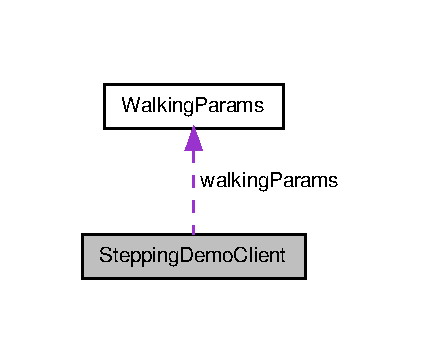
\includegraphics[width=203pt]{classSteppingDemoClient__coll__graph}
\end{center}
\end{figure}
\subsection*{\-Public \-Member \-Functions}
\begin{DoxyCompactItemize}
\item 
\hyperlink{classSteppingDemoClient_a28e41547ba5641741ceb3b378a5983db}{\-Stepping\-Demo\-Client} (std\-::shared\-\_\-ptr$<$ ocra\-::\-Model $>$ model\-Ptr, const int loop\-Period)
\item 
virtual \hyperlink{classSteppingDemoClient_a573eed904c7262c5cdbaf6e254d72559}{$\sim$\-Stepping\-Demo\-Client} ()
\end{DoxyCompactItemize}
\subsection*{\-Public \-Attributes}
\begin{DoxyCompactItemize}
\item 
\hyperlink{SteppingDemoClient_8h_abd6d177d63e98aa1b4ed4b8329e2a379}{\-M\-O\-T\-I\-O\-N\-\_\-\-T\-Y\-P\-E} \hyperlink{classSteppingDemoClient_aa880debbcbed0298ae1769dd8a3f721b}{motion\-Type}
\end{DoxyCompactItemize}
\subsection*{\-Protected \-Member \-Functions}
\begin{DoxyCompactItemize}
\item 
virtual bool \hyperlink{classSteppingDemoClient_a08dce195eece162eed175ac9487667c2}{initialize} ()
\item 
virtual void \hyperlink{classSteppingDemoClient_aafcb227c0d7ce24823957e2331caa88b}{release} ()
\item 
virtual void \hyperlink{classSteppingDemoClient_a37dba4764b5849cf33c395cd0d4b0eb5}{loop} ()
\end{DoxyCompactItemize}
\subsection*{\-Private \-Member \-Functions}
\begin{DoxyCompactItemize}
\item 
void \hyperlink{classSteppingDemoClient_a0f6b689c5f032351484b03e71a3530e1}{static\-Walking\-Loop} ()
\item 
void \hyperlink{classSteppingDemoClient_a94b990ae53b1b40ef8f9469b427d171c}{left\-To\-Right\-Loop} ()
\item 
\-Eigen\-::\-Vector3d \hyperlink{classSteppingDemoClient_af6a814243828f5136476aa5e99ea0079}{get\-Left\-Foot\-Position} ()
\item 
\-Eigen\-::\-Vector3d \hyperlink{classSteppingDemoClient_ae9c0d72756c109f49c269a7e1b06454a}{get\-Right\-Foot\-Position} ()
\item 
\-Eigen\-::\-Vector3d \hyperlink{classSteppingDemoClient_a857aa530a4ab94443d0b0869121baf76}{get\-Co\-M\-Position} ()
\item 
void \hyperlink{classSteppingDemoClient_a18609e5634a283423c228106bb0e3a45}{position\-Co\-M\-Over} (\hyperlink{SteppingDemoClient_8h_ac0c3848a609566394821d9826e0fdd5b}{\-C\-O\-M\-\_\-\-S\-U\-P\-P\-O\-R\-T\-\_\-\-P\-O\-S\-I\-T\-I\-O\-N} new\-Support\-Pos)
\item 
bool \hyperlink{classSteppingDemoClient_ad8fbc186267a47a73bb77e78199f2b8c}{is\-Balanced} ()
\item 
void \hyperlink{classSteppingDemoClient_a62b5028bdc99de117cfffc576478a0f1}{deactivate\-Foot\-Contacts} (\hyperlink{SteppingDemoClient_8h_ab0673d7f17cdd57b8fa124abb330287f}{\-F\-O\-O\-T\-\_\-\-C\-O\-N\-T\-A\-C\-T\-S} foot)
\item 
void \hyperlink{classSteppingDemoClient_abf583698c8c03620516acf3ec6eb9e41}{activate\-Foot\-Contacts} (\hyperlink{SteppingDemoClient_8h_ab0673d7f17cdd57b8fa124abb330287f}{\-F\-O\-O\-T\-\_\-\-C\-O\-N\-T\-A\-C\-T\-S} foot)
\item 
bool \hyperlink{classSteppingDemoClient_aeeaa9fac47e3e5a141647b07fa2feaa3}{is\-Foot\-In\-Contact} (\hyperlink{SteppingDemoClient_8h_ab0673d7f17cdd57b8fa124abb330287f}{\-F\-O\-O\-T\-\_\-\-C\-O\-N\-T\-A\-C\-T\-S} foot)
\item 
void \hyperlink{classSteppingDemoClient_a6b5d8bf0ce08c8b9f66ac2c1bbd5bcd7}{pause\-For} (double \-\_\-pause\-Duration)
\item 
bool \hyperlink{classSteppingDemoClient_afe78b799d8b8c63cff7d1e8765b7e1fa}{pause\-Finished} ()
\item 
bool \hyperlink{classSteppingDemoClient_ae406e5c8f755f234272b63de4d6a774f}{lift\-Foot} (\hyperlink{SteppingDemoClient_8h_ab0673d7f17cdd57b8fa124abb330287f}{\-F\-O\-O\-T\-\_\-\-C\-O\-N\-T\-A\-C\-T\-S} foot, bool is\-Left\-Foot\-In\-Contact, bool is\-Right\-Foot\-In\-Contact)
\item 
bool \hyperlink{classSteppingDemoClient_a930123dad5658ea8a3bb5f23cb4cb369}{set\-Down\-Foot} (\hyperlink{SteppingDemoClient_8h_ab0673d7f17cdd57b8fa124abb330287f}{\-F\-O\-O\-T\-\_\-\-C\-O\-N\-T\-A\-C\-T\-S} foot)
\item 
void \hyperlink{classSteppingDemoClient_a346a8fd10641897532a26f598db7799d}{state\-Machine\-With\-Pause\-In\-Double\-Support} ()
\item 
void \hyperlink{classSteppingDemoClient_a256284578a6b9818a8f726451d2fb2c4}{state\-Machine\-Without\-Pause\-In\-Double\-Support} ()
\end{DoxyCompactItemize}
\subsection*{\-Private \-Attributes}
\begin{DoxyCompactItemize}
\item 
ocra\-\_\-recipes\-::\-Task\-Connection\-::\-Ptr \hyperlink{classSteppingDemoClient_a5dd71720cd8f7a17d21f74d20b3c23ff}{\-Left\-Foot\-Contact\-\_\-\-Back\-Left}
\item 
ocra\-\_\-recipes\-::\-Task\-Connection\-::\-Ptr \hyperlink{classSteppingDemoClient_a32e69816ec216b3d6502385e2346d22d}{\-Left\-Foot\-Contact\-\_\-\-Front\-Left}
\item 
ocra\-\_\-recipes\-::\-Task\-Connection\-::\-Ptr \hyperlink{classSteppingDemoClient_a946ab9de6d55274e5cb9b9a8743a30b8}{\-Left\-Foot\-Contact\-\_\-\-Back\-Right}
\item 
ocra\-\_\-recipes\-::\-Task\-Connection\-::\-Ptr \hyperlink{classSteppingDemoClient_ae2c0ca1ba0ef69b5f09fd3cd982fb772}{\-Left\-Foot\-Contact\-\_\-\-Front\-Right}
\item 
ocra\-\_\-recipes\-::\-Task\-Connection\-::\-Ptr \hyperlink{classSteppingDemoClient_aaaf5dee15bf151def4b4070751d1ca84}{\-Right\-Foot\-Contact\-\_\-\-Back\-Left}
\item 
ocra\-\_\-recipes\-::\-Task\-Connection\-::\-Ptr \hyperlink{classSteppingDemoClient_ad10f639e025b003fd383f4cc933da15f}{\-Right\-Foot\-Contact\-\_\-\-Front\-Left}
\item 
ocra\-\_\-recipes\-::\-Task\-Connection\-::\-Ptr \hyperlink{classSteppingDemoClient_a93e209732588c3ef2b04e39e3df40d3e}{\-Right\-Foot\-Contact\-\_\-\-Back\-Right}
\item 
ocra\-\_\-recipes\-::\-Task\-Connection\-::\-Ptr \hyperlink{classSteppingDemoClient_a781be1c0ffd7e7147eb2b2de66ba3231}{\-Right\-Foot\-Contact\-\_\-\-Front\-Right}
\item 
double \hyperlink{classSteppingDemoClient_a13a5deff16d52936f788bb9b0af6e9c9}{pause\-Trigger\-Time}
\item 
double \hyperlink{classSteppingDemoClient_a92b810b2d2c50e359da18e5d91163340}{pause\-Duration}
\item 
double \hyperlink{classSteppingDemoClient_a1bb7d42cf09778349ae1ecd31d2ac116}{current\-Time}
\item 
bool \hyperlink{classSteppingDemoClient_a29e7765300c7d2e2d5108025fbdcbc2c}{is\-Pausing}
\item 
bool \hyperlink{classSteppingDemoClient_a88b84ed8fc7808ea3fb68f2ec3d29ebe}{is\-In\-Left\-Support\-Mode}
\item 
bool \hyperlink{classSteppingDemoClient_a7697070e5db6c635aa2eff70bce29176}{is\-In\-Right\-Support\-Mode}
\item 
bool \hyperlink{classSteppingDemoClient_a6036e2d0b604648ca39e4d64b41a9d6e}{foot\-Trajectory\-Started}
\item 
std\-::shared\-\_\-ptr\*
$<$ ocra\-\_\-recipes\-::\-Trajectory\-Thread $>$ \hyperlink{classSteppingDemoClient_afd18627088c2c12f172ff9e976da5330}{left\-Foot\-\_\-\-Traj\-Thread}
\item 
std\-::shared\-\_\-ptr\*
$<$ ocra\-\_\-recipes\-::\-Trajectory\-Thread $>$ \hyperlink{classSteppingDemoClient_a8b4b931d41b47d9923417506fac107f3}{right\-Foot\-\_\-\-Traj\-Thread}
\item 
std\-::shared\-\_\-ptr\*
$<$ ocra\-\_\-recipes\-::\-Trajectory\-Thread $>$ \hyperlink{classSteppingDemoClient_a9f3d1cdc49cc26a10f9b8fb0d0c68cab}{com\-\_\-\-Traj\-Thread}
\item 
\-Eigen\-::\-Vector3d \hyperlink{classSteppingDemoClient_acd4cb9dbe053979701574f5d1d4ef349}{left\-Foot\-Home}
\item 
\-Eigen\-::\-Vector3d \hyperlink{classSteppingDemoClient_ae2a3bdaafc7784b5afece8ae9ebaff7d}{right\-Foot\-Home}
\item 
\-Eigen\-::\-Vector3d \hyperlink{classSteppingDemoClient_aa018c1f2734d63f962be512461c9e010}{com\-Home}
\item 
\-Eigen\-::\-Vector3d \hyperlink{classSteppingDemoClient_a2360933e2902d1b1a374787bd67e14e7}{left\-Foot\-Target}
\item 
\-Eigen\-::\-Vector3d \hyperlink{classSteppingDemoClient_abfe6635a0ad50fa4baa6fa10b8c56d9e}{right\-Foot\-Target}
\item 
\-Eigen\-::\-Vector3d \hyperlink{classSteppingDemoClient_af9e0358390f12ed0135275b20bf1f6f5}{next\-Step}
\item 
\-Eigen\-::\-Vector3d \hyperlink{classSteppingDemoClient_ab4a77111abbf3630280a64d17ac59eef}{new\-Co\-M\-Goal\-Position}
\item 
double \hyperlink{classSteppingDemoClient_af7b6e48319ef9d35fb975edc3bb2a137}{start\-Time}
\item 
bool \hyperlink{classSteppingDemoClient_aedd8bb5bca60afbdd2b8de3b5d1829d7}{get\-Initial\-Values}
\item 
\hyperlink{SteppingDemoClient_8h_af2a8507bf21c3ce9b0e67a23381251c6}{\-C\-O\-N\-T\-R\-O\-L\-\_\-\-P\-H\-A\-S\-E} \hyperlink{classSteppingDemoClient_afe0aa2a02ea8117d644bf5444a03ac62}{current\-Phase}
\item 
\hyperlink{SteppingDemoClient_8h_af2a8507bf21c3ce9b0e67a23381251c6}{\-C\-O\-N\-T\-R\-O\-L\-\_\-\-P\-H\-A\-S\-E} \hyperlink{classSteppingDemoClient_ab5a3b82049a9786162a60d0ae94f96d9}{next\-Phase}
\item 
bool \hyperlink{classSteppingDemoClient_ad7e3950d053af7c1aca33b3e7c3b20c5}{is\-Moving\-Co\-M}
\item 
\hyperlink{structWalkingParams}{\-Walking\-Params} \hyperlink{classSteppingDemoClient_a113c2d838e3db1d18f4843a8828e30d4}{walking\-Params}
\end{DoxyCompactItemize}


\subsection{\-Constructor \& \-Destructor \-Documentation}
\hypertarget{classSteppingDemoClient_a28e41547ba5641741ceb3b378a5983db}{\index{\-Stepping\-Demo\-Client@{\-Stepping\-Demo\-Client}!\-Stepping\-Demo\-Client@{\-Stepping\-Demo\-Client}}
\index{\-Stepping\-Demo\-Client@{\-Stepping\-Demo\-Client}!SteppingDemoClient@{\-Stepping\-Demo\-Client}}
\subsubsection[{\-Stepping\-Demo\-Client}]{\setlength{\rightskip}{0pt plus 5cm}{\bf \-Stepping\-Demo\-Client\-::\-Stepping\-Demo\-Client} (
\begin{DoxyParamCaption}
\item[{std\-::shared\-\_\-ptr$<$ ocra\-::\-Model $>$}]{model\-Ptr, }
\item[{const int}]{loop\-Period}
\end{DoxyParamCaption}
)}}\label{classSteppingDemoClient_a28e41547ba5641741ceb3b378a5983db}
\hypertarget{classSteppingDemoClient_a573eed904c7262c5cdbaf6e254d72559}{\index{\-Stepping\-Demo\-Client@{\-Stepping\-Demo\-Client}!$\sim$\-Stepping\-Demo\-Client@{$\sim$\-Stepping\-Demo\-Client}}
\index{$\sim$\-Stepping\-Demo\-Client@{$\sim$\-Stepping\-Demo\-Client}!SteppingDemoClient@{\-Stepping\-Demo\-Client}}
\subsubsection[{$\sim$\-Stepping\-Demo\-Client}]{\setlength{\rightskip}{0pt plus 5cm}{\bf \-Stepping\-Demo\-Client\-::$\sim$\-Stepping\-Demo\-Client} (
\begin{DoxyParamCaption}
{}
\end{DoxyParamCaption}
)\hspace{0.3cm}{\ttfamily  \mbox{[}virtual\mbox{]}}}}\label{classSteppingDemoClient_a573eed904c7262c5cdbaf6e254d72559}


\subsection{\-Member \-Function \-Documentation}
\hypertarget{classSteppingDemoClient_abf583698c8c03620516acf3ec6eb9e41}{\index{\-Stepping\-Demo\-Client@{\-Stepping\-Demo\-Client}!activate\-Foot\-Contacts@{activate\-Foot\-Contacts}}
\index{activate\-Foot\-Contacts@{activate\-Foot\-Contacts}!SteppingDemoClient@{\-Stepping\-Demo\-Client}}
\subsubsection[{activate\-Foot\-Contacts}]{\setlength{\rightskip}{0pt plus 5cm}void {\bf \-Stepping\-Demo\-Client\-::activate\-Foot\-Contacts} (
\begin{DoxyParamCaption}
\item[{{\bf \-F\-O\-O\-T\-\_\-\-C\-O\-N\-T\-A\-C\-T\-S}}]{foot}
\end{DoxyParamCaption}
)\hspace{0.3cm}{\ttfamily  \mbox{[}private\mbox{]}}}}\label{classSteppingDemoClient_abf583698c8c03620516acf3ec6eb9e41}
\-This method asks the ocra-\/icub-\/server to activate one by one the feet \char`\"{}corner\char`\"{} contact tasks for the specified foot.


\begin{DoxyParams}{\-Parameters}
{\em foot} & \-L\-E\-F\-T\-\_\-\-F\-O\-O\-T or \-R\-I\-G\-H\-T\-\_\-\-F\-O\-O\-T. \\
\hline
\end{DoxyParams}
\hypertarget{classSteppingDemoClient_a62b5028bdc99de117cfffc576478a0f1}{\index{\-Stepping\-Demo\-Client@{\-Stepping\-Demo\-Client}!deactivate\-Foot\-Contacts@{deactivate\-Foot\-Contacts}}
\index{deactivate\-Foot\-Contacts@{deactivate\-Foot\-Contacts}!SteppingDemoClient@{\-Stepping\-Demo\-Client}}
\subsubsection[{deactivate\-Foot\-Contacts}]{\setlength{\rightskip}{0pt plus 5cm}void {\bf \-Stepping\-Demo\-Client\-::deactivate\-Foot\-Contacts} (
\begin{DoxyParamCaption}
\item[{{\bf \-F\-O\-O\-T\-\_\-\-C\-O\-N\-T\-A\-C\-T\-S}}]{foot}
\end{DoxyParamCaption}
)\hspace{0.3cm}{\ttfamily  \mbox{[}private\mbox{]}}}}\label{classSteppingDemoClient_a62b5028bdc99de117cfffc576478a0f1}
\-Remember the right and left feet contact tasks? created in \hyperlink{classSteppingDemoClient_a08dce195eece162eed175ac9487667c2}{initialize()}. \-This method acts the ocra-\/icub-\/server to deactivate one by one the feet \char`\"{}corner\char`\"{} contact tasks for the specified foot.


\begin{DoxyParams}{\-Parameters}
{\em foot} & \-L\-E\-F\-T\-\_\-\-F\-O\-O\-T or \-R\-I\-G\-H\-T\-\_\-\-F\-O\-O\-T. \\
\hline
\end{DoxyParams}
\hypertarget{classSteppingDemoClient_a857aa530a4ab94443d0b0869121baf76}{\index{\-Stepping\-Demo\-Client@{\-Stepping\-Demo\-Client}!get\-Co\-M\-Position@{get\-Co\-M\-Position}}
\index{get\-Co\-M\-Position@{get\-Co\-M\-Position}!SteppingDemoClient@{\-Stepping\-Demo\-Client}}
\subsubsection[{get\-Co\-M\-Position}]{\setlength{\rightskip}{0pt plus 5cm}\-Eigen\-::\-Vector3d {\bf \-Stepping\-Demo\-Client\-::get\-Co\-M\-Position} (
\begin{DoxyParamCaption}
{}
\end{DoxyParamCaption}
)\hspace{0.3cm}{\ttfamily  \mbox{[}private\mbox{]}}}}\label{classSteppingDemoClient_a857aa530a4ab94443d0b0869121baf76}
\-Retrieves the 3\-D position of the \char`\"{}\-Co\-M\char`\"{} as done by the yarp\-Whole\-Body\-Interface.

\begin{DoxyReturn}{\-Returns}
3\-D position of the \-C\-O\-M. 
\end{DoxyReturn}
\hypertarget{classSteppingDemoClient_af6a814243828f5136476aa5e99ea0079}{\index{\-Stepping\-Demo\-Client@{\-Stepping\-Demo\-Client}!get\-Left\-Foot\-Position@{get\-Left\-Foot\-Position}}
\index{get\-Left\-Foot\-Position@{get\-Left\-Foot\-Position}!SteppingDemoClient@{\-Stepping\-Demo\-Client}}
\subsubsection[{get\-Left\-Foot\-Position}]{\setlength{\rightskip}{0pt plus 5cm}\-Eigen\-::\-Vector3d {\bf \-Stepping\-Demo\-Client\-::get\-Left\-Foot\-Position} (
\begin{DoxyParamCaption}
{}
\end{DoxyParamCaption}
)\hspace{0.3cm}{\ttfamily  \mbox{[}private\mbox{]}}}}\label{classSteppingDemoClient_af6a814243828f5136476aa5e99ea0079}
\-Retrieves the 3\-D position of the \char`\"{}l\-\_\-sole\char`\"{} frame from the i\-Cub model.

\begin{DoxyReturn}{\-Returns}
3\-D position of the left foot. 
\end{DoxyReturn}
\hypertarget{classSteppingDemoClient_ae9c0d72756c109f49c269a7e1b06454a}{\index{\-Stepping\-Demo\-Client@{\-Stepping\-Demo\-Client}!get\-Right\-Foot\-Position@{get\-Right\-Foot\-Position}}
\index{get\-Right\-Foot\-Position@{get\-Right\-Foot\-Position}!SteppingDemoClient@{\-Stepping\-Demo\-Client}}
\subsubsection[{get\-Right\-Foot\-Position}]{\setlength{\rightskip}{0pt plus 5cm}\-Eigen\-::\-Vector3d {\bf \-Stepping\-Demo\-Client\-::get\-Right\-Foot\-Position} (
\begin{DoxyParamCaption}
{}
\end{DoxyParamCaption}
)\hspace{0.3cm}{\ttfamily  \mbox{[}private\mbox{]}}}}\label{classSteppingDemoClient_ae9c0d72756c109f49c269a7e1b06454a}
\-Retrieves the 3\-D position of the \char`\"{}r\-\_\-sole\char`\"{} frame from the i\-Cub model.

\begin{DoxyReturn}{\-Returns}
3\-D position of the right foot. 
\end{DoxyReturn}
\hypertarget{classSteppingDemoClient_a08dce195eece162eed175ac9487667c2}{\index{\-Stepping\-Demo\-Client@{\-Stepping\-Demo\-Client}!initialize@{initialize}}
\index{initialize@{initialize}!SteppingDemoClient@{\-Stepping\-Demo\-Client}}
\subsubsection[{initialize}]{\setlength{\rightskip}{0pt plus 5cm}bool {\bf \-Stepping\-Demo\-Client\-::initialize} (
\begin{DoxyParamCaption}
{}
\end{DoxyParamCaption}
)\hspace{0.3cm}{\ttfamily  \mbox{[}protected, virtual\mbox{]}}}}\label{classSteppingDemoClient_a08dce195eece162eed175ac9487667c2}
\-The initialization consists of the following\-: 1. \-Defines trajectory types (e.\-g. \-Min. \-Jerk) 2. \-Defines the termination strategy 3. \-Instantiates trajectory threads for the left and right foot as well as for the \-Co\-M, sets them up (max velocity, error threshold) and finally starts them. 4. \-Instantiates ocra\-::\-Task\-Connection objects for the left and right feet contacts (4 per foot on each corner).


\begin{DoxyItemize}
\item returns\-: \-True if everything has been initialized properly, false otherwise. 
\end{DoxyItemize}\hypertarget{classSteppingDemoClient_ad8fbc186267a47a73bb77e78199f2b8c}{\index{\-Stepping\-Demo\-Client@{\-Stepping\-Demo\-Client}!is\-Balanced@{is\-Balanced}}
\index{is\-Balanced@{is\-Balanced}!SteppingDemoClient@{\-Stepping\-Demo\-Client}}
\subsubsection[{is\-Balanced}]{\setlength{\rightskip}{0pt plus 5cm}bool {\bf \-Stepping\-Demo\-Client\-::is\-Balanced} (
\begin{DoxyParamCaption}
{}
\end{DoxyParamCaption}
)\hspace{0.3cm}{\ttfamily  \mbox{[}private\mbox{]}}}}\label{classSteppingDemoClient_ad8fbc186267a47a73bb77e78199f2b8c}
\-Uses the norm of the \-C\-O\-M and joint velocities to understand if the robot is balanced.

\begin{DoxyReturn}{\-Returns}
\-True when both the norm of the \-C\-O\-M and joint velocities are below com\-Vel\-Threshold and joint\-Threshold. 
\end{DoxyReturn}
\begin{DoxyRefDesc}{\-Todo}
\item[\hyperlink{todo__todo000002}{\-Todo}]\-A more balance-\/centered criterion should be used for this, \-Z\-M\-P-\/based for example. \end{DoxyRefDesc}
\hypertarget{classSteppingDemoClient_aeeaa9fac47e3e5a141647b07fa2feaa3}{\index{\-Stepping\-Demo\-Client@{\-Stepping\-Demo\-Client}!is\-Foot\-In\-Contact@{is\-Foot\-In\-Contact}}
\index{is\-Foot\-In\-Contact@{is\-Foot\-In\-Contact}!SteppingDemoClient@{\-Stepping\-Demo\-Client}}
\subsubsection[{is\-Foot\-In\-Contact}]{\setlength{\rightskip}{0pt plus 5cm}bool {\bf \-Stepping\-Demo\-Client\-::is\-Foot\-In\-Contact} (
\begin{DoxyParamCaption}
\item[{{\bf \-F\-O\-O\-T\-\_\-\-C\-O\-N\-T\-A\-C\-T\-S}}]{foot}
\end{DoxyParamCaption}
)\hspace{0.3cm}{\ttfamily  \mbox{[}private\mbox{]}}}}\label{classSteppingDemoClient_aeeaa9fac47e3e5a141647b07fa2feaa3}
\-If the foot height is less than or equal to foot\-Contact\-Release\-Threshold, the feet contacts tasks are activated.


\begin{DoxyParams}{\-Parameters}
{\em foot} & \-L\-E\-F\-T\-\_\-\-F\-O\-O\-T or \-R\-I\-G\-H\-T\-\_\-\-F\-O\-O\-T.\\
\hline
\end{DoxyParams}
\begin{DoxyReturn}{\-Returns}
\-True if the activation of the contact happens successfully. \-False if the foot's elevation is not under the foot\-Contact\-Release\-Threshold. 
\end{DoxyReturn}
\hypertarget{classSteppingDemoClient_a94b990ae53b1b40ef8f9469b427d171c}{\index{\-Stepping\-Demo\-Client@{\-Stepping\-Demo\-Client}!left\-To\-Right\-Loop@{left\-To\-Right\-Loop}}
\index{left\-To\-Right\-Loop@{left\-To\-Right\-Loop}!SteppingDemoClient@{\-Stepping\-Demo\-Client}}
\subsubsection[{left\-To\-Right\-Loop}]{\setlength{\rightskip}{0pt plus 5cm}void {\bf \-Stepping\-Demo\-Client\-::left\-To\-Right\-Loop} (
\begin{DoxyParamCaption}
{}
\end{DoxyParamCaption}
)\hspace{0.3cm}{\ttfamily  \mbox{[}private\mbox{]}}}}\label{classSteppingDemoClient_a94b990ae53b1b40ef8f9469b427d171c}
\hypertarget{classSteppingDemoClient_ae406e5c8f755f234272b63de4d6a774f}{\index{\-Stepping\-Demo\-Client@{\-Stepping\-Demo\-Client}!lift\-Foot@{lift\-Foot}}
\index{lift\-Foot@{lift\-Foot}!SteppingDemoClient@{\-Stepping\-Demo\-Client}}
\subsubsection[{lift\-Foot}]{\setlength{\rightskip}{0pt plus 5cm}bool {\bf \-Stepping\-Demo\-Client\-::lift\-Foot} (
\begin{DoxyParamCaption}
\item[{{\bf \-F\-O\-O\-T\-\_\-\-C\-O\-N\-T\-A\-C\-T\-S}}]{foot, }
\item[{bool}]{is\-Left\-Foot\-In\-Contact, }
\item[{bool}]{is\-Right\-Foot\-In\-Contact}
\end{DoxyParamCaption}
)\hspace{0.3cm}{\ttfamily  \mbox{[}private\mbox{]}}}}\label{classSteppingDemoClient_ae406e5c8f755f234272b63de4d6a774f}
\-Sets the right or left foot waypoint to right\-Foot\-Target or left\-Foot\-Target accordingly (where the foot will be lifted). \-These values are harcoded in the \hyperlink{classSteppingDemoClient_a37dba4764b5849cf33c395cd0d4b0eb5}{loop()} method and updated only during the very first iteration when the variable get\-Initial\-Values is set to true.


\begin{DoxyParams}{\-Parameters}
{\em foot} & \-L\-E\-F\-T\-\_\-\-F\-O\-O\-T or \-R\-I\-G\-H\-T\-\_\-\-F\-O\-O\-T \\
\hline
{\em is\-Left\-Foot\-In\-Contact} & \-Updates the current state of the left foot contact. \\
\hline
{\em is\-Right\-Foot\-In\-Contact} & \-Updates the current state of the right foot contact.\\
\hline
\end{DoxyParams}
\begin{DoxyReturn}{\-Returns}
\-True after the foot contact is deactivated. 
\end{DoxyReturn}
\hypertarget{classSteppingDemoClient_a37dba4764b5849cf33c395cd0d4b0eb5}{\index{\-Stepping\-Demo\-Client@{\-Stepping\-Demo\-Client}!loop@{loop}}
\index{loop@{loop}!SteppingDemoClient@{\-Stepping\-Demo\-Client}}
\subsubsection[{loop}]{\setlength{\rightskip}{0pt plus 5cm}void {\bf \-Stepping\-Demo\-Client\-::loop} (
\begin{DoxyParamCaption}
{}
\end{DoxyParamCaption}
)\hspace{0.3cm}{\ttfamily  \mbox{[}protected, virtual\mbox{]}}}}\label{classSteppingDemoClient_a37dba4764b5849cf33c395cd0d4b0eb5}
\-Initially waits for two seconds, to make sure that all model states have been correctly updated during the initialization. \-During the first loop it retrieves left and right feet positions along with the com's. \hypertarget{classSteppingDemoClient_afe78b799d8b8c63cff7d1e8765b7e1fa}{\index{\-Stepping\-Demo\-Client@{\-Stepping\-Demo\-Client}!pause\-Finished@{pause\-Finished}}
\index{pause\-Finished@{pause\-Finished}!SteppingDemoClient@{\-Stepping\-Demo\-Client}}
\subsubsection[{pause\-Finished}]{\setlength{\rightskip}{0pt plus 5cm}bool {\bf \-Stepping\-Demo\-Client\-::pause\-Finished} (
\begin{DoxyParamCaption}
{}
\end{DoxyParamCaption}
)\hspace{0.3cm}{\ttfamily  \mbox{[}private\mbox{]}}}}\label{classSteppingDemoClient_afe78b799d8b8c63cff7d1e8765b7e1fa}
\-Sets is\-Pausing to false when pause\-Duration has passed.

\begin{DoxyReturn}{\-Returns}
\-True when the pause duration is over. \-False otherwise. 
\end{DoxyReturn}
\hypertarget{classSteppingDemoClient_a6b5d8bf0ce08c8b9f66ac2c1bbd5bcd7}{\index{\-Stepping\-Demo\-Client@{\-Stepping\-Demo\-Client}!pause\-For@{pause\-For}}
\index{pause\-For@{pause\-For}!SteppingDemoClient@{\-Stepping\-Demo\-Client}}
\subsubsection[{pause\-For}]{\setlength{\rightskip}{0pt plus 5cm}void {\bf \-Stepping\-Demo\-Client\-::pause\-For} (
\begin{DoxyParamCaption}
\item[{double}]{\-\_\-pause\-Duration}
\end{DoxyParamCaption}
)\hspace{0.3cm}{\ttfamily  \mbox{[}private\mbox{]}}}}\label{classSteppingDemoClient_a6b5d8bf0ce08c8b9f66ac2c1bbd5bcd7}
\-Mainly sets is\-Pausing to true and stores the time at which the pause was called.


\begin{DoxyParams}{\-Parameters}
{\em \-\_\-pause\-Duration} & \-Pause duration. \\
\hline
\end{DoxyParams}
\hypertarget{classSteppingDemoClient_a18609e5634a283423c228106bb0e3a45}{\index{\-Stepping\-Demo\-Client@{\-Stepping\-Demo\-Client}!position\-Co\-M\-Over@{position\-Co\-M\-Over}}
\index{position\-Co\-M\-Over@{position\-Co\-M\-Over}!SteppingDemoClient@{\-Stepping\-Demo\-Client}}
\subsubsection[{position\-Co\-M\-Over}]{\setlength{\rightskip}{0pt plus 5cm}void {\bf \-Stepping\-Demo\-Client\-::position\-Co\-M\-Over} (
\begin{DoxyParamCaption}
\item[{{\bf \-C\-O\-M\-\_\-\-S\-U\-P\-P\-O\-R\-T\-\_\-\-P\-O\-S\-I\-T\-I\-O\-N}}]{new\-Support\-Pos}
\end{DoxyParamCaption}
)\hspace{0.3cm}{\ttfamily  \mbox{[}private\mbox{]}}}}\label{classSteppingDemoClient_a18609e5634a283423c228106bb0e3a45}
\-Sets \-C\-O\-M trajectory waypoints according to the desired support position\-: \-L\-E\-F\-T\-\_\-\-F\-O\-O\-T\-\_\-\-X\-Y\-: \-The \-C\-O\-M goal position is set to be on top of the left foot. \-R\-I\-G\-H\-T\-\_\-\-F\-O\-O\-T\-\_\-\-X\-Y\-: \-The \-C\-O\-M goal position is set to be on top of the right foot. \-C\-E\-N\-T\-E\-R\-E\-D\-\_\-\-B\-E\-T\-W\-E\-E\-N\-\_\-\-F\-E\-E\-T\-\_\-\-X\-Y\-: \-The \-C\-O\-M goal position is set between both feet. \-The height of the com is always the current \-C\-O\-M's height. \-Since the thread must have started before calling this method, it will update the current waypoint trajectory it has or start it.


\begin{DoxyParams}{\-Parameters}
{\em new\-Support\-Pos} & \-New support position. \\
\hline
\end{DoxyParams}
\hypertarget{classSteppingDemoClient_aafcb227c0d7ce24823957e2331caa88b}{\index{\-Stepping\-Demo\-Client@{\-Stepping\-Demo\-Client}!release@{release}}
\index{release@{release}!SteppingDemoClient@{\-Stepping\-Demo\-Client}}
\subsubsection[{release}]{\setlength{\rightskip}{0pt plus 5cm}void {\bf \-Stepping\-Demo\-Client\-::release} (
\begin{DoxyParamCaption}
{}
\end{DoxyParamCaption}
)\hspace{0.3cm}{\ttfamily  \mbox{[}protected, virtual\mbox{]}}}}\label{classSteppingDemoClient_aafcb227c0d7ce24823957e2331caa88b}
\-Stops the trajectory threads of the \-Co\-M, left and right feet. \hypertarget{classSteppingDemoClient_a930123dad5658ea8a3bb5f23cb4cb369}{\index{\-Stepping\-Demo\-Client@{\-Stepping\-Demo\-Client}!set\-Down\-Foot@{set\-Down\-Foot}}
\index{set\-Down\-Foot@{set\-Down\-Foot}!SteppingDemoClient@{\-Stepping\-Demo\-Client}}
\subsubsection[{set\-Down\-Foot}]{\setlength{\rightskip}{0pt plus 5cm}bool {\bf \-Stepping\-Demo\-Client\-::set\-Down\-Foot} (
\begin{DoxyParamCaption}
\item[{{\bf \-F\-O\-O\-T\-\_\-\-C\-O\-N\-T\-A\-C\-T\-S}}]{foot}
\end{DoxyParamCaption}
)\hspace{0.3cm}{\ttfamily  \mbox{[}private\mbox{]}}}}\label{classSteppingDemoClient_a930123dad5658ea8a3bb5f23cb4cb369}
\-Sets the right or left foot waypoint to right\-Foot\-Home or left\-Foot\-Home accordingly (where the foot will land). \-These values are harcoded in the \hyperlink{classSteppingDemoClient_a37dba4764b5849cf33c395cd0d4b0eb5}{loop()} method and updated only during the very first iteration when the variable get\-Initial\-Values is set to true.


\begin{DoxyParams}{\-Parameters}
{\em foot} & \-L\-E\-F\-T\-\_\-\-F\-O\-O\-T or \-R\-I\-G\-H\-T\-\_\-\-F\-O\-O\-T\\
\hline
\end{DoxyParams}
\begin{DoxyReturn}{\-Returns}
\-True only after the foot has established contact again and the trajectory is over. \-False while the foot is still moving back down looking for contact or simply, the goal hasn't been attained. 
\end{DoxyReturn}
\hypertarget{classSteppingDemoClient_a256284578a6b9818a8f726451d2fb2c4}{\index{\-Stepping\-Demo\-Client@{\-Stepping\-Demo\-Client}!state\-Machine\-Without\-Pause\-In\-Double\-Support@{state\-Machine\-Without\-Pause\-In\-Double\-Support}}
\index{state\-Machine\-Without\-Pause\-In\-Double\-Support@{state\-Machine\-Without\-Pause\-In\-Double\-Support}!SteppingDemoClient@{\-Stepping\-Demo\-Client}}
\subsubsection[{state\-Machine\-Without\-Pause\-In\-Double\-Support}]{\setlength{\rightskip}{0pt plus 5cm}void {\bf \-Stepping\-Demo\-Client\-::state\-Machine\-Without\-Pause\-In\-Double\-Support} (
\begin{DoxyParamCaption}
{}
\end{DoxyParamCaption}
)\hspace{0.3cm}{\ttfamily  \mbox{[}private\mbox{]}}}}\label{classSteppingDemoClient_a256284578a6b9818a8f726451d2fb2c4}
\hypertarget{classSteppingDemoClient_a346a8fd10641897532a26f598db7799d}{\index{\-Stepping\-Demo\-Client@{\-Stepping\-Demo\-Client}!state\-Machine\-With\-Pause\-In\-Double\-Support@{state\-Machine\-With\-Pause\-In\-Double\-Support}}
\index{state\-Machine\-With\-Pause\-In\-Double\-Support@{state\-Machine\-With\-Pause\-In\-Double\-Support}!SteppingDemoClient@{\-Stepping\-Demo\-Client}}
\subsubsection[{state\-Machine\-With\-Pause\-In\-Double\-Support}]{\setlength{\rightskip}{0pt plus 5cm}void {\bf \-Stepping\-Demo\-Client\-::state\-Machine\-With\-Pause\-In\-Double\-Support} (
\begin{DoxyParamCaption}
{}
\end{DoxyParamCaption}
)\hspace{0.3cm}{\ttfamily  \mbox{[}private\mbox{]}}}}\label{classSteppingDemoClient_a346a8fd10641897532a26f598db7799d}
\hypertarget{classSteppingDemoClient_a0f6b689c5f032351484b03e71a3530e1}{\index{\-Stepping\-Demo\-Client@{\-Stepping\-Demo\-Client}!static\-Walking\-Loop@{static\-Walking\-Loop}}
\index{static\-Walking\-Loop@{static\-Walking\-Loop}!SteppingDemoClient@{\-Stepping\-Demo\-Client}}
\subsubsection[{static\-Walking\-Loop}]{\setlength{\rightskip}{0pt plus 5cm}void {\bf \-Stepping\-Demo\-Client\-::static\-Walking\-Loop} (
\begin{DoxyParamCaption}
{}
\end{DoxyParamCaption}
)\hspace{0.3cm}{\ttfamily  \mbox{[}private\mbox{]}}}}\label{classSteppingDemoClient_a0f6b689c5f032351484b03e71a3530e1}


\subsection{\-Member \-Data \-Documentation}
\hypertarget{classSteppingDemoClient_a9f3d1cdc49cc26a10f9b8fb0d0c68cab}{\index{\-Stepping\-Demo\-Client@{\-Stepping\-Demo\-Client}!com\-\_\-\-Traj\-Thread@{com\-\_\-\-Traj\-Thread}}
\index{com\-\_\-\-Traj\-Thread@{com\-\_\-\-Traj\-Thread}!SteppingDemoClient@{\-Stepping\-Demo\-Client}}
\subsubsection[{com\-\_\-\-Traj\-Thread}]{\setlength{\rightskip}{0pt plus 5cm}std\-::shared\-\_\-ptr$<$ocra\-\_\-recipes\-::\-Trajectory\-Thread$>$ {\bf \-Stepping\-Demo\-Client\-::com\-\_\-\-Traj\-Thread}\hspace{0.3cm}{\ttfamily  \mbox{[}private\mbox{]}}}}\label{classSteppingDemoClient_a9f3d1cdc49cc26a10f9b8fb0d0c68cab}
\hypertarget{classSteppingDemoClient_aa018c1f2734d63f962be512461c9e010}{\index{\-Stepping\-Demo\-Client@{\-Stepping\-Demo\-Client}!com\-Home@{com\-Home}}
\index{com\-Home@{com\-Home}!SteppingDemoClient@{\-Stepping\-Demo\-Client}}
\subsubsection[{com\-Home}]{\setlength{\rightskip}{0pt plus 5cm}\-Eigen\-::\-Vector3d {\bf \-Stepping\-Demo\-Client\-::com\-Home}\hspace{0.3cm}{\ttfamily  \mbox{[}private\mbox{]}}}}\label{classSteppingDemoClient_aa018c1f2734d63f962be512461c9e010}
\hypertarget{classSteppingDemoClient_afe0aa2a02ea8117d644bf5444a03ac62}{\index{\-Stepping\-Demo\-Client@{\-Stepping\-Demo\-Client}!current\-Phase@{current\-Phase}}
\index{current\-Phase@{current\-Phase}!SteppingDemoClient@{\-Stepping\-Demo\-Client}}
\subsubsection[{current\-Phase}]{\setlength{\rightskip}{0pt plus 5cm}{\bf \-C\-O\-N\-T\-R\-O\-L\-\_\-\-P\-H\-A\-S\-E} {\bf \-Stepping\-Demo\-Client\-::current\-Phase}\hspace{0.3cm}{\ttfamily  \mbox{[}private\mbox{]}}}}\label{classSteppingDemoClient_afe0aa2a02ea8117d644bf5444a03ac62}
\hypertarget{classSteppingDemoClient_a1bb7d42cf09778349ae1ecd31d2ac116}{\index{\-Stepping\-Demo\-Client@{\-Stepping\-Demo\-Client}!current\-Time@{current\-Time}}
\index{current\-Time@{current\-Time}!SteppingDemoClient@{\-Stepping\-Demo\-Client}}
\subsubsection[{current\-Time}]{\setlength{\rightskip}{0pt plus 5cm}double {\bf \-Stepping\-Demo\-Client\-::current\-Time}\hspace{0.3cm}{\ttfamily  \mbox{[}private\mbox{]}}}}\label{classSteppingDemoClient_a1bb7d42cf09778349ae1ecd31d2ac116}
\hypertarget{classSteppingDemoClient_a6036e2d0b604648ca39e4d64b41a9d6e}{\index{\-Stepping\-Demo\-Client@{\-Stepping\-Demo\-Client}!foot\-Trajectory\-Started@{foot\-Trajectory\-Started}}
\index{foot\-Trajectory\-Started@{foot\-Trajectory\-Started}!SteppingDemoClient@{\-Stepping\-Demo\-Client}}
\subsubsection[{foot\-Trajectory\-Started}]{\setlength{\rightskip}{0pt plus 5cm}bool {\bf \-Stepping\-Demo\-Client\-::foot\-Trajectory\-Started}\hspace{0.3cm}{\ttfamily  \mbox{[}private\mbox{]}}}}\label{classSteppingDemoClient_a6036e2d0b604648ca39e4d64b41a9d6e}
\hypertarget{classSteppingDemoClient_aedd8bb5bca60afbdd2b8de3b5d1829d7}{\index{\-Stepping\-Demo\-Client@{\-Stepping\-Demo\-Client}!get\-Initial\-Values@{get\-Initial\-Values}}
\index{get\-Initial\-Values@{get\-Initial\-Values}!SteppingDemoClient@{\-Stepping\-Demo\-Client}}
\subsubsection[{get\-Initial\-Values}]{\setlength{\rightskip}{0pt plus 5cm}bool {\bf \-Stepping\-Demo\-Client\-::get\-Initial\-Values}\hspace{0.3cm}{\ttfamily  \mbox{[}private\mbox{]}}}}\label{classSteppingDemoClient_aedd8bb5bca60afbdd2b8de3b5d1829d7}
\hypertarget{classSteppingDemoClient_a88b84ed8fc7808ea3fb68f2ec3d29ebe}{\index{\-Stepping\-Demo\-Client@{\-Stepping\-Demo\-Client}!is\-In\-Left\-Support\-Mode@{is\-In\-Left\-Support\-Mode}}
\index{is\-In\-Left\-Support\-Mode@{is\-In\-Left\-Support\-Mode}!SteppingDemoClient@{\-Stepping\-Demo\-Client}}
\subsubsection[{is\-In\-Left\-Support\-Mode}]{\setlength{\rightskip}{0pt plus 5cm}bool {\bf \-Stepping\-Demo\-Client\-::is\-In\-Left\-Support\-Mode}\hspace{0.3cm}{\ttfamily  \mbox{[}private\mbox{]}}}}\label{classSteppingDemoClient_a88b84ed8fc7808ea3fb68f2ec3d29ebe}
\hypertarget{classSteppingDemoClient_a7697070e5db6c635aa2eff70bce29176}{\index{\-Stepping\-Demo\-Client@{\-Stepping\-Demo\-Client}!is\-In\-Right\-Support\-Mode@{is\-In\-Right\-Support\-Mode}}
\index{is\-In\-Right\-Support\-Mode@{is\-In\-Right\-Support\-Mode}!SteppingDemoClient@{\-Stepping\-Demo\-Client}}
\subsubsection[{is\-In\-Right\-Support\-Mode}]{\setlength{\rightskip}{0pt plus 5cm}bool {\bf \-Stepping\-Demo\-Client\-::is\-In\-Right\-Support\-Mode}\hspace{0.3cm}{\ttfamily  \mbox{[}private\mbox{]}}}}\label{classSteppingDemoClient_a7697070e5db6c635aa2eff70bce29176}
\hypertarget{classSteppingDemoClient_ad7e3950d053af7c1aca33b3e7c3b20c5}{\index{\-Stepping\-Demo\-Client@{\-Stepping\-Demo\-Client}!is\-Moving\-Co\-M@{is\-Moving\-Co\-M}}
\index{is\-Moving\-Co\-M@{is\-Moving\-Co\-M}!SteppingDemoClient@{\-Stepping\-Demo\-Client}}
\subsubsection[{is\-Moving\-Co\-M}]{\setlength{\rightskip}{0pt plus 5cm}bool {\bf \-Stepping\-Demo\-Client\-::is\-Moving\-Co\-M}\hspace{0.3cm}{\ttfamily  \mbox{[}private\mbox{]}}}}\label{classSteppingDemoClient_ad7e3950d053af7c1aca33b3e7c3b20c5}
\hypertarget{classSteppingDemoClient_a29e7765300c7d2e2d5108025fbdcbc2c}{\index{\-Stepping\-Demo\-Client@{\-Stepping\-Demo\-Client}!is\-Pausing@{is\-Pausing}}
\index{is\-Pausing@{is\-Pausing}!SteppingDemoClient@{\-Stepping\-Demo\-Client}}
\subsubsection[{is\-Pausing}]{\setlength{\rightskip}{0pt plus 5cm}bool {\bf \-Stepping\-Demo\-Client\-::is\-Pausing}\hspace{0.3cm}{\ttfamily  \mbox{[}private\mbox{]}}}}\label{classSteppingDemoClient_a29e7765300c7d2e2d5108025fbdcbc2c}
\hypertarget{classSteppingDemoClient_afd18627088c2c12f172ff9e976da5330}{\index{\-Stepping\-Demo\-Client@{\-Stepping\-Demo\-Client}!left\-Foot\-\_\-\-Traj\-Thread@{left\-Foot\-\_\-\-Traj\-Thread}}
\index{left\-Foot\-\_\-\-Traj\-Thread@{left\-Foot\-\_\-\-Traj\-Thread}!SteppingDemoClient@{\-Stepping\-Demo\-Client}}
\subsubsection[{left\-Foot\-\_\-\-Traj\-Thread}]{\setlength{\rightskip}{0pt plus 5cm}std\-::shared\-\_\-ptr$<$ocra\-\_\-recipes\-::\-Trajectory\-Thread$>$ {\bf \-Stepping\-Demo\-Client\-::left\-Foot\-\_\-\-Traj\-Thread}\hspace{0.3cm}{\ttfamily  \mbox{[}private\mbox{]}}}}\label{classSteppingDemoClient_afd18627088c2c12f172ff9e976da5330}
\hypertarget{classSteppingDemoClient_a5dd71720cd8f7a17d21f74d20b3c23ff}{\index{\-Stepping\-Demo\-Client@{\-Stepping\-Demo\-Client}!\-Left\-Foot\-Contact\-\_\-\-Back\-Left@{\-Left\-Foot\-Contact\-\_\-\-Back\-Left}}
\index{\-Left\-Foot\-Contact\-\_\-\-Back\-Left@{\-Left\-Foot\-Contact\-\_\-\-Back\-Left}!SteppingDemoClient@{\-Stepping\-Demo\-Client}}
\subsubsection[{\-Left\-Foot\-Contact\-\_\-\-Back\-Left}]{\setlength{\rightskip}{0pt plus 5cm}ocra\-\_\-recipes\-::\-Task\-Connection\-::\-Ptr {\bf \-Stepping\-Demo\-Client\-::\-Left\-Foot\-Contact\-\_\-\-Back\-Left}\hspace{0.3cm}{\ttfamily  \mbox{[}private\mbox{]}}}}\label{classSteppingDemoClient_a5dd71720cd8f7a17d21f74d20b3c23ff}
\hypertarget{classSteppingDemoClient_a946ab9de6d55274e5cb9b9a8743a30b8}{\index{\-Stepping\-Demo\-Client@{\-Stepping\-Demo\-Client}!\-Left\-Foot\-Contact\-\_\-\-Back\-Right@{\-Left\-Foot\-Contact\-\_\-\-Back\-Right}}
\index{\-Left\-Foot\-Contact\-\_\-\-Back\-Right@{\-Left\-Foot\-Contact\-\_\-\-Back\-Right}!SteppingDemoClient@{\-Stepping\-Demo\-Client}}
\subsubsection[{\-Left\-Foot\-Contact\-\_\-\-Back\-Right}]{\setlength{\rightskip}{0pt plus 5cm}ocra\-\_\-recipes\-::\-Task\-Connection\-::\-Ptr {\bf \-Stepping\-Demo\-Client\-::\-Left\-Foot\-Contact\-\_\-\-Back\-Right}\hspace{0.3cm}{\ttfamily  \mbox{[}private\mbox{]}}}}\label{classSteppingDemoClient_a946ab9de6d55274e5cb9b9a8743a30b8}
\hypertarget{classSteppingDemoClient_a32e69816ec216b3d6502385e2346d22d}{\index{\-Stepping\-Demo\-Client@{\-Stepping\-Demo\-Client}!\-Left\-Foot\-Contact\-\_\-\-Front\-Left@{\-Left\-Foot\-Contact\-\_\-\-Front\-Left}}
\index{\-Left\-Foot\-Contact\-\_\-\-Front\-Left@{\-Left\-Foot\-Contact\-\_\-\-Front\-Left}!SteppingDemoClient@{\-Stepping\-Demo\-Client}}
\subsubsection[{\-Left\-Foot\-Contact\-\_\-\-Front\-Left}]{\setlength{\rightskip}{0pt plus 5cm}ocra\-\_\-recipes\-::\-Task\-Connection\-::\-Ptr {\bf \-Stepping\-Demo\-Client\-::\-Left\-Foot\-Contact\-\_\-\-Front\-Left}\hspace{0.3cm}{\ttfamily  \mbox{[}private\mbox{]}}}}\label{classSteppingDemoClient_a32e69816ec216b3d6502385e2346d22d}
\hypertarget{classSteppingDemoClient_ae2c0ca1ba0ef69b5f09fd3cd982fb772}{\index{\-Stepping\-Demo\-Client@{\-Stepping\-Demo\-Client}!\-Left\-Foot\-Contact\-\_\-\-Front\-Right@{\-Left\-Foot\-Contact\-\_\-\-Front\-Right}}
\index{\-Left\-Foot\-Contact\-\_\-\-Front\-Right@{\-Left\-Foot\-Contact\-\_\-\-Front\-Right}!SteppingDemoClient@{\-Stepping\-Demo\-Client}}
\subsubsection[{\-Left\-Foot\-Contact\-\_\-\-Front\-Right}]{\setlength{\rightskip}{0pt plus 5cm}ocra\-\_\-recipes\-::\-Task\-Connection\-::\-Ptr {\bf \-Stepping\-Demo\-Client\-::\-Left\-Foot\-Contact\-\_\-\-Front\-Right}\hspace{0.3cm}{\ttfamily  \mbox{[}private\mbox{]}}}}\label{classSteppingDemoClient_ae2c0ca1ba0ef69b5f09fd3cd982fb772}
\hypertarget{classSteppingDemoClient_acd4cb9dbe053979701574f5d1d4ef349}{\index{\-Stepping\-Demo\-Client@{\-Stepping\-Demo\-Client}!left\-Foot\-Home@{left\-Foot\-Home}}
\index{left\-Foot\-Home@{left\-Foot\-Home}!SteppingDemoClient@{\-Stepping\-Demo\-Client}}
\subsubsection[{left\-Foot\-Home}]{\setlength{\rightskip}{0pt plus 5cm}\-Eigen\-::\-Vector3d {\bf \-Stepping\-Demo\-Client\-::left\-Foot\-Home}\hspace{0.3cm}{\ttfamily  \mbox{[}private\mbox{]}}}}\label{classSteppingDemoClient_acd4cb9dbe053979701574f5d1d4ef349}
\hypertarget{classSteppingDemoClient_a2360933e2902d1b1a374787bd67e14e7}{\index{\-Stepping\-Demo\-Client@{\-Stepping\-Demo\-Client}!left\-Foot\-Target@{left\-Foot\-Target}}
\index{left\-Foot\-Target@{left\-Foot\-Target}!SteppingDemoClient@{\-Stepping\-Demo\-Client}}
\subsubsection[{left\-Foot\-Target}]{\setlength{\rightskip}{0pt plus 5cm}\-Eigen\-::\-Vector3d {\bf \-Stepping\-Demo\-Client\-::left\-Foot\-Target}\hspace{0.3cm}{\ttfamily  \mbox{[}private\mbox{]}}}}\label{classSteppingDemoClient_a2360933e2902d1b1a374787bd67e14e7}
\hypertarget{classSteppingDemoClient_aa880debbcbed0298ae1769dd8a3f721b}{\index{\-Stepping\-Demo\-Client@{\-Stepping\-Demo\-Client}!motion\-Type@{motion\-Type}}
\index{motion\-Type@{motion\-Type}!SteppingDemoClient@{\-Stepping\-Demo\-Client}}
\subsubsection[{motion\-Type}]{\setlength{\rightskip}{0pt plus 5cm}{\bf \-M\-O\-T\-I\-O\-N\-\_\-\-T\-Y\-P\-E} {\bf \-Stepping\-Demo\-Client\-::motion\-Type}}}\label{classSteppingDemoClient_aa880debbcbed0298ae1769dd8a3f721b}
\hypertarget{classSteppingDemoClient_ab4a77111abbf3630280a64d17ac59eef}{\index{\-Stepping\-Demo\-Client@{\-Stepping\-Demo\-Client}!new\-Co\-M\-Goal\-Position@{new\-Co\-M\-Goal\-Position}}
\index{new\-Co\-M\-Goal\-Position@{new\-Co\-M\-Goal\-Position}!SteppingDemoClient@{\-Stepping\-Demo\-Client}}
\subsubsection[{new\-Co\-M\-Goal\-Position}]{\setlength{\rightskip}{0pt plus 5cm}\-Eigen\-::\-Vector3d {\bf \-Stepping\-Demo\-Client\-::new\-Co\-M\-Goal\-Position}\hspace{0.3cm}{\ttfamily  \mbox{[}private\mbox{]}}}}\label{classSteppingDemoClient_ab4a77111abbf3630280a64d17ac59eef}
\hypertarget{classSteppingDemoClient_ab5a3b82049a9786162a60d0ae94f96d9}{\index{\-Stepping\-Demo\-Client@{\-Stepping\-Demo\-Client}!next\-Phase@{next\-Phase}}
\index{next\-Phase@{next\-Phase}!SteppingDemoClient@{\-Stepping\-Demo\-Client}}
\subsubsection[{next\-Phase}]{\setlength{\rightskip}{0pt plus 5cm}{\bf \-C\-O\-N\-T\-R\-O\-L\-\_\-\-P\-H\-A\-S\-E} {\bf \-Stepping\-Demo\-Client\-::next\-Phase}\hspace{0.3cm}{\ttfamily  \mbox{[}private\mbox{]}}}}\label{classSteppingDemoClient_ab5a3b82049a9786162a60d0ae94f96d9}
\hypertarget{classSteppingDemoClient_af9e0358390f12ed0135275b20bf1f6f5}{\index{\-Stepping\-Demo\-Client@{\-Stepping\-Demo\-Client}!next\-Step@{next\-Step}}
\index{next\-Step@{next\-Step}!SteppingDemoClient@{\-Stepping\-Demo\-Client}}
\subsubsection[{next\-Step}]{\setlength{\rightskip}{0pt plus 5cm}\-Eigen\-::\-Vector3d {\bf \-Stepping\-Demo\-Client\-::next\-Step}\hspace{0.3cm}{\ttfamily  \mbox{[}private\mbox{]}}}}\label{classSteppingDemoClient_af9e0358390f12ed0135275b20bf1f6f5}
\hypertarget{classSteppingDemoClient_a92b810b2d2c50e359da18e5d91163340}{\index{\-Stepping\-Demo\-Client@{\-Stepping\-Demo\-Client}!pause\-Duration@{pause\-Duration}}
\index{pause\-Duration@{pause\-Duration}!SteppingDemoClient@{\-Stepping\-Demo\-Client}}
\subsubsection[{pause\-Duration}]{\setlength{\rightskip}{0pt plus 5cm}double {\bf \-Stepping\-Demo\-Client\-::pause\-Duration}\hspace{0.3cm}{\ttfamily  \mbox{[}private\mbox{]}}}}\label{classSteppingDemoClient_a92b810b2d2c50e359da18e5d91163340}
\hypertarget{classSteppingDemoClient_a13a5deff16d52936f788bb9b0af6e9c9}{\index{\-Stepping\-Demo\-Client@{\-Stepping\-Demo\-Client}!pause\-Trigger\-Time@{pause\-Trigger\-Time}}
\index{pause\-Trigger\-Time@{pause\-Trigger\-Time}!SteppingDemoClient@{\-Stepping\-Demo\-Client}}
\subsubsection[{pause\-Trigger\-Time}]{\setlength{\rightskip}{0pt plus 5cm}double {\bf \-Stepping\-Demo\-Client\-::pause\-Trigger\-Time}\hspace{0.3cm}{\ttfamily  \mbox{[}private\mbox{]}}}}\label{classSteppingDemoClient_a13a5deff16d52936f788bb9b0af6e9c9}
\hypertarget{classSteppingDemoClient_a8b4b931d41b47d9923417506fac107f3}{\index{\-Stepping\-Demo\-Client@{\-Stepping\-Demo\-Client}!right\-Foot\-\_\-\-Traj\-Thread@{right\-Foot\-\_\-\-Traj\-Thread}}
\index{right\-Foot\-\_\-\-Traj\-Thread@{right\-Foot\-\_\-\-Traj\-Thread}!SteppingDemoClient@{\-Stepping\-Demo\-Client}}
\subsubsection[{right\-Foot\-\_\-\-Traj\-Thread}]{\setlength{\rightskip}{0pt plus 5cm}std\-::shared\-\_\-ptr$<$ocra\-\_\-recipes\-::\-Trajectory\-Thread$>$ {\bf \-Stepping\-Demo\-Client\-::right\-Foot\-\_\-\-Traj\-Thread}\hspace{0.3cm}{\ttfamily  \mbox{[}private\mbox{]}}}}\label{classSteppingDemoClient_a8b4b931d41b47d9923417506fac107f3}
\hypertarget{classSteppingDemoClient_aaaf5dee15bf151def4b4070751d1ca84}{\index{\-Stepping\-Demo\-Client@{\-Stepping\-Demo\-Client}!\-Right\-Foot\-Contact\-\_\-\-Back\-Left@{\-Right\-Foot\-Contact\-\_\-\-Back\-Left}}
\index{\-Right\-Foot\-Contact\-\_\-\-Back\-Left@{\-Right\-Foot\-Contact\-\_\-\-Back\-Left}!SteppingDemoClient@{\-Stepping\-Demo\-Client}}
\subsubsection[{\-Right\-Foot\-Contact\-\_\-\-Back\-Left}]{\setlength{\rightskip}{0pt plus 5cm}ocra\-\_\-recipes\-::\-Task\-Connection\-::\-Ptr {\bf \-Stepping\-Demo\-Client\-::\-Right\-Foot\-Contact\-\_\-\-Back\-Left}\hspace{0.3cm}{\ttfamily  \mbox{[}private\mbox{]}}}}\label{classSteppingDemoClient_aaaf5dee15bf151def4b4070751d1ca84}
\hypertarget{classSteppingDemoClient_a93e209732588c3ef2b04e39e3df40d3e}{\index{\-Stepping\-Demo\-Client@{\-Stepping\-Demo\-Client}!\-Right\-Foot\-Contact\-\_\-\-Back\-Right@{\-Right\-Foot\-Contact\-\_\-\-Back\-Right}}
\index{\-Right\-Foot\-Contact\-\_\-\-Back\-Right@{\-Right\-Foot\-Contact\-\_\-\-Back\-Right}!SteppingDemoClient@{\-Stepping\-Demo\-Client}}
\subsubsection[{\-Right\-Foot\-Contact\-\_\-\-Back\-Right}]{\setlength{\rightskip}{0pt plus 5cm}ocra\-\_\-recipes\-::\-Task\-Connection\-::\-Ptr {\bf \-Stepping\-Demo\-Client\-::\-Right\-Foot\-Contact\-\_\-\-Back\-Right}\hspace{0.3cm}{\ttfamily  \mbox{[}private\mbox{]}}}}\label{classSteppingDemoClient_a93e209732588c3ef2b04e39e3df40d3e}
\hypertarget{classSteppingDemoClient_ad10f639e025b003fd383f4cc933da15f}{\index{\-Stepping\-Demo\-Client@{\-Stepping\-Demo\-Client}!\-Right\-Foot\-Contact\-\_\-\-Front\-Left@{\-Right\-Foot\-Contact\-\_\-\-Front\-Left}}
\index{\-Right\-Foot\-Contact\-\_\-\-Front\-Left@{\-Right\-Foot\-Contact\-\_\-\-Front\-Left}!SteppingDemoClient@{\-Stepping\-Demo\-Client}}
\subsubsection[{\-Right\-Foot\-Contact\-\_\-\-Front\-Left}]{\setlength{\rightskip}{0pt plus 5cm}ocra\-\_\-recipes\-::\-Task\-Connection\-::\-Ptr {\bf \-Stepping\-Demo\-Client\-::\-Right\-Foot\-Contact\-\_\-\-Front\-Left}\hspace{0.3cm}{\ttfamily  \mbox{[}private\mbox{]}}}}\label{classSteppingDemoClient_ad10f639e025b003fd383f4cc933da15f}
\hypertarget{classSteppingDemoClient_a781be1c0ffd7e7147eb2b2de66ba3231}{\index{\-Stepping\-Demo\-Client@{\-Stepping\-Demo\-Client}!\-Right\-Foot\-Contact\-\_\-\-Front\-Right@{\-Right\-Foot\-Contact\-\_\-\-Front\-Right}}
\index{\-Right\-Foot\-Contact\-\_\-\-Front\-Right@{\-Right\-Foot\-Contact\-\_\-\-Front\-Right}!SteppingDemoClient@{\-Stepping\-Demo\-Client}}
\subsubsection[{\-Right\-Foot\-Contact\-\_\-\-Front\-Right}]{\setlength{\rightskip}{0pt plus 5cm}ocra\-\_\-recipes\-::\-Task\-Connection\-::\-Ptr {\bf \-Stepping\-Demo\-Client\-::\-Right\-Foot\-Contact\-\_\-\-Front\-Right}\hspace{0.3cm}{\ttfamily  \mbox{[}private\mbox{]}}}}\label{classSteppingDemoClient_a781be1c0ffd7e7147eb2b2de66ba3231}
\hypertarget{classSteppingDemoClient_ae2a3bdaafc7784b5afece8ae9ebaff7d}{\index{\-Stepping\-Demo\-Client@{\-Stepping\-Demo\-Client}!right\-Foot\-Home@{right\-Foot\-Home}}
\index{right\-Foot\-Home@{right\-Foot\-Home}!SteppingDemoClient@{\-Stepping\-Demo\-Client}}
\subsubsection[{right\-Foot\-Home}]{\setlength{\rightskip}{0pt plus 5cm}\-Eigen\-::\-Vector3d {\bf \-Stepping\-Demo\-Client\-::right\-Foot\-Home}\hspace{0.3cm}{\ttfamily  \mbox{[}private\mbox{]}}}}\label{classSteppingDemoClient_ae2a3bdaafc7784b5afece8ae9ebaff7d}
\hypertarget{classSteppingDemoClient_abfe6635a0ad50fa4baa6fa10b8c56d9e}{\index{\-Stepping\-Demo\-Client@{\-Stepping\-Demo\-Client}!right\-Foot\-Target@{right\-Foot\-Target}}
\index{right\-Foot\-Target@{right\-Foot\-Target}!SteppingDemoClient@{\-Stepping\-Demo\-Client}}
\subsubsection[{right\-Foot\-Target}]{\setlength{\rightskip}{0pt plus 5cm}\-Eigen\-::\-Vector3d {\bf \-Stepping\-Demo\-Client\-::right\-Foot\-Target}\hspace{0.3cm}{\ttfamily  \mbox{[}private\mbox{]}}}}\label{classSteppingDemoClient_abfe6635a0ad50fa4baa6fa10b8c56d9e}
\hypertarget{classSteppingDemoClient_af7b6e48319ef9d35fb975edc3bb2a137}{\index{\-Stepping\-Demo\-Client@{\-Stepping\-Demo\-Client}!start\-Time@{start\-Time}}
\index{start\-Time@{start\-Time}!SteppingDemoClient@{\-Stepping\-Demo\-Client}}
\subsubsection[{start\-Time}]{\setlength{\rightskip}{0pt plus 5cm}double {\bf \-Stepping\-Demo\-Client\-::start\-Time}\hspace{0.3cm}{\ttfamily  \mbox{[}private\mbox{]}}}}\label{classSteppingDemoClient_af7b6e48319ef9d35fb975edc3bb2a137}
\hypertarget{classSteppingDemoClient_a113c2d838e3db1d18f4843a8828e30d4}{\index{\-Stepping\-Demo\-Client@{\-Stepping\-Demo\-Client}!walking\-Params@{walking\-Params}}
\index{walking\-Params@{walking\-Params}!SteppingDemoClient@{\-Stepping\-Demo\-Client}}
\subsubsection[{walking\-Params}]{\setlength{\rightskip}{0pt plus 5cm}{\bf \-Walking\-Params} {\bf \-Stepping\-Demo\-Client\-::walking\-Params}\hspace{0.3cm}{\ttfamily  \mbox{[}private\mbox{]}}}}\label{classSteppingDemoClient_a113c2d838e3db1d18f4843a8828e30d4}


\-The documentation for this class was generated from the following files\-:\begin{DoxyCompactItemize}
\item 
ocra-\/wbi-\/plugins/ocra-\/icub-\/clients/stepping-\/demo/include/stepping-\/demo/\hyperlink{SteppingDemoClient_8h}{\-Stepping\-Demo\-Client.\-h}\item 
ocra-\/wbi-\/plugins/ocra-\/icub-\/clients/stepping-\/demo/src/\hyperlink{SteppingDemoClient_8cpp}{\-Stepping\-Demo\-Client.\-cpp}\end{DoxyCompactItemize}

\hypertarget{classTaskOpsClient}{\section{\-Task\-Ops\-Client \-Class \-Reference}
\label{classTaskOpsClient}\index{\-Task\-Ops\-Client@{\-Task\-Ops\-Client}}
}


{\ttfamily \#include $<$\-Task\-Ops\-Client.\-h$>$}

\subsection*{\-Public \-Member \-Functions}
\begin{DoxyCompactItemize}
\item 
\hyperlink{classTaskOpsClient_a6d3842de3255a78526ced7953428452c}{\-Task\-Ops\-Client} (std\-::shared\-\_\-ptr$<$ ocra\-::\-Model $>$ model\-Ptr, const int loop\-Period)
\item 
virtual \hyperlink{classTaskOpsClient_a80a5c71dd04ab7a07d4ffb8116244cdd}{$\sim$\-Task\-Ops\-Client} ()
\end{DoxyCompactItemize}
\subsection*{\-Protected \-Member \-Functions}
\begin{DoxyCompactItemize}
\item 
virtual bool \hyperlink{classTaskOpsClient_a6f5e4c20c1d5f5df28dcc58e3cb4adb0}{initialize} ()
\item 
virtual void \hyperlink{classTaskOpsClient_af54d37bc4a2631c5c47e23d8156f6e95}{release} ()
\item 
virtual void \hyperlink{classTaskOpsClient_a7e7dfab7af0404f0b008da2844ab573e}{loop} ()
\end{DoxyCompactItemize}
\subsection*{\-Private \-Attributes}
\begin{DoxyCompactItemize}
\item 
\hyperlink{TaskOpsClient_8h_a0140057ae3fbe1db5f5c418dfc67d9db}{\-T\-H\-I\-N\-G\-S\-\_\-\-T\-O\-\_\-\-D\-O} \hyperlink{classTaskOpsClient_a3409c4ef6b396943397b5bd9237f0a40}{thing\-To\-Do}
\end{DoxyCompactItemize}


\subsection{\-Constructor \& \-Destructor \-Documentation}
\hypertarget{classTaskOpsClient_a6d3842de3255a78526ced7953428452c}{\index{\-Task\-Ops\-Client@{\-Task\-Ops\-Client}!\-Task\-Ops\-Client@{\-Task\-Ops\-Client}}
\index{\-Task\-Ops\-Client@{\-Task\-Ops\-Client}!TaskOpsClient@{\-Task\-Ops\-Client}}
\subsubsection[{\-Task\-Ops\-Client}]{\setlength{\rightskip}{0pt plus 5cm}{\bf \-Task\-Ops\-Client\-::\-Task\-Ops\-Client} (
\begin{DoxyParamCaption}
\item[{std\-::shared\-\_\-ptr$<$ ocra\-::\-Model $>$}]{model\-Ptr, }
\item[{const int}]{loop\-Period}
\end{DoxyParamCaption}
)}}\label{classTaskOpsClient_a6d3842de3255a78526ced7953428452c}
\hypertarget{classTaskOpsClient_a80a5c71dd04ab7a07d4ffb8116244cdd}{\index{\-Task\-Ops\-Client@{\-Task\-Ops\-Client}!$\sim$\-Task\-Ops\-Client@{$\sim$\-Task\-Ops\-Client}}
\index{$\sim$\-Task\-Ops\-Client@{$\sim$\-Task\-Ops\-Client}!TaskOpsClient@{\-Task\-Ops\-Client}}
\subsubsection[{$\sim$\-Task\-Ops\-Client}]{\setlength{\rightskip}{0pt plus 5cm}{\bf \-Task\-Ops\-Client\-::$\sim$\-Task\-Ops\-Client} (
\begin{DoxyParamCaption}
{}
\end{DoxyParamCaption}
)\hspace{0.3cm}{\ttfamily  \mbox{[}virtual\mbox{]}}}}\label{classTaskOpsClient_a80a5c71dd04ab7a07d4ffb8116244cdd}


\subsection{\-Member \-Function \-Documentation}
\hypertarget{classTaskOpsClient_a6f5e4c20c1d5f5df28dcc58e3cb4adb0}{\index{\-Task\-Ops\-Client@{\-Task\-Ops\-Client}!initialize@{initialize}}
\index{initialize@{initialize}!TaskOpsClient@{\-Task\-Ops\-Client}}
\subsubsection[{initialize}]{\setlength{\rightskip}{0pt plus 5cm}bool {\bf \-Task\-Ops\-Client\-::initialize} (
\begin{DoxyParamCaption}
{}
\end{DoxyParamCaption}
)\hspace{0.3cm}{\ttfamily  \mbox{[}protected, virtual\mbox{]}}}}\label{classTaskOpsClient_a6f5e4c20c1d5f5df28dcc58e3cb4adb0}
\hypertarget{classTaskOpsClient_a7e7dfab7af0404f0b008da2844ab573e}{\index{\-Task\-Ops\-Client@{\-Task\-Ops\-Client}!loop@{loop}}
\index{loop@{loop}!TaskOpsClient@{\-Task\-Ops\-Client}}
\subsubsection[{loop}]{\setlength{\rightskip}{0pt plus 5cm}void {\bf \-Task\-Ops\-Client\-::loop} (
\begin{DoxyParamCaption}
{}
\end{DoxyParamCaption}
)\hspace{0.3cm}{\ttfamily  \mbox{[}protected, virtual\mbox{]}}}}\label{classTaskOpsClient_a7e7dfab7af0404f0b008da2844ab573e}
\hypertarget{classTaskOpsClient_af54d37bc4a2631c5c47e23d8156f6e95}{\index{\-Task\-Ops\-Client@{\-Task\-Ops\-Client}!release@{release}}
\index{release@{release}!TaskOpsClient@{\-Task\-Ops\-Client}}
\subsubsection[{release}]{\setlength{\rightskip}{0pt plus 5cm}void {\bf \-Task\-Ops\-Client\-::release} (
\begin{DoxyParamCaption}
{}
\end{DoxyParamCaption}
)\hspace{0.3cm}{\ttfamily  \mbox{[}protected, virtual\mbox{]}}}}\label{classTaskOpsClient_af54d37bc4a2631c5c47e23d8156f6e95}


\subsection{\-Member \-Data \-Documentation}
\hypertarget{classTaskOpsClient_a3409c4ef6b396943397b5bd9237f0a40}{\index{\-Task\-Ops\-Client@{\-Task\-Ops\-Client}!thing\-To\-Do@{thing\-To\-Do}}
\index{thing\-To\-Do@{thing\-To\-Do}!TaskOpsClient@{\-Task\-Ops\-Client}}
\subsubsection[{thing\-To\-Do}]{\setlength{\rightskip}{0pt plus 5cm}{\bf \-T\-H\-I\-N\-G\-S\-\_\-\-T\-O\-\_\-\-D\-O} {\bf \-Task\-Ops\-Client\-::thing\-To\-Do}\hspace{0.3cm}{\ttfamily  \mbox{[}private\mbox{]}}}}\label{classTaskOpsClient_a3409c4ef6b396943397b5bd9237f0a40}


\-The documentation for this class was generated from the following files\-:\begin{DoxyCompactItemize}
\item 
ocra-\/wbi-\/plugins/ocra-\/icub-\/clients/task-\/operations-\/demo/include/task-\/operations-\/demo/\hyperlink{TaskOpsClient_8h}{\-Task\-Ops\-Client.\-h}\item 
ocra-\/wbi-\/plugins/ocra-\/icub-\/clients/task-\/operations-\/demo/src/\hyperlink{TaskOpsClient_8cpp}{\-Task\-Ops\-Client.\-cpp}\end{DoxyCompactItemize}

\hypertarget{classThread}{\section{\-Thread \-Class \-Reference}
\label{classThread}\index{\-Thread@{\-Thread}}
}


\-The meat and potatoes of the controller server.  




{\ttfamily \#include $<$\-Thread.\-h$>$}



\-Collaboration diagram for \-Thread\-:\nopagebreak
\begin{figure}[H]
\begin{center}
\leavevmode
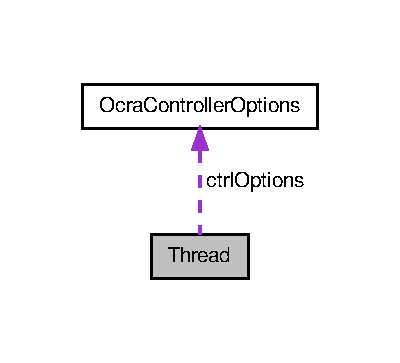
\includegraphics[width=192pt]{classThread__coll__graph}
\end{center}
\end{figure}
\subsection*{\-Classes}
\begin{DoxyCompactItemize}
\item 
class \hyperlink{classThread_1_1ControllerRpcServerCallback}{\-Controller\-Rpc\-Server\-Callback}
\begin{DoxyCompactList}\small\item\em \-A callback function which binds the rpc server port opened in the contoller server module to the controller thread's parsing function. \end{DoxyCompactList}\item 
class \hyperlink{classThread_1_1DebugRpcServerCallback}{\-Debug\-Rpc\-Server\-Callback}
\begin{DoxyCompactList}\small\item\em \-A callback function which binds the rpc server port opened in the contoller server module to the controller thread's parsing function. \end{DoxyCompactList}\end{DoxyCompactItemize}
\subsection*{\-Public \-Member \-Functions}
\begin{DoxyCompactItemize}
\item 
\hyperlink{classThread_a7494a3cf676527432ee724d59ed9ee8f}{\-Thread} (\hyperlink{classOcraControllerOptions}{\-Ocra\-Controller\-Options} \&controller\-\_\-options, std\-::shared\-\_\-ptr$<$ wbi\-::whole\-Body\-Interface $>$ wbi)
\item 
virtual \hyperlink{classThread_a37d9edd3a1a776cbc27dedff949c9726}{$\sim$\-Thread} ()
\item 
bool \hyperlink{classThread_a1e840470cd71d7bfb2430d24169e3dce}{thread\-Init} ()
\item 
void \hyperlink{classThread_ad9373d8d725c46717dfce3130018fe3a}{run} ()
\item 
void \hyperlink{classThread_aa2856c7d45670f45d66bcb319255defe}{thread\-Release} ()
\end{DoxyCompactItemize}
\subsection*{\-Private \-Member \-Functions}
\begin{DoxyCompactItemize}
\item 
\hyperlink{namespaceocra__icub_afbd2db66b68005fb7cfac19210caf83f}{ocra\-\_\-icub\-::\-O\-C\-R\-A\-\_\-\-I\-C\-U\-B\-\_\-\-M\-E\-S\-S\-A\-G\-E} \hyperlink{classThread_a2c64d83df66f7168d34993b76a179dde}{convert\-String\-To\-Ocra\-Icub\-Message} (const std\-::string \&s)
\item 
void \hyperlink{classThread_ae21029d250ac7c720f2411eab71a9414}{parse\-Incoming\-Message} (yarp\-::os\-::\-Bottle \&input, yarp\-::os\-::\-Bottle \&reply)
\item 
void \hyperlink{classThread_a6ce5ef9684cb2793be85e7402ad672f0}{parse\-Debug\-Message} (yarp\-::os\-::\-Bottle \&input, yarp\-::os\-::\-Bottle \&reply)
\item 
void \hyperlink{classThread_a9af0e98aa9b1de2f5c7bfa2f6e5001a2}{write\-Debug\-Data} ()
\item 
void \hyperlink{classThread_a49b65da88eb521ff53ef94d6ec8da7ab}{put\-Ankles\-Into\-Idle} ()
\end{DoxyCompactItemize}
\subsection*{\-Private \-Attributes}
\begin{DoxyCompactItemize}
\item 
ocra\-::\-Model\-::\-Ptr \hyperlink{classThread_a1dcef9aedc1a707e6f04d5fb6e4a0b13}{model}
\item 
std\-::shared\-\_\-ptr\*
$<$ \hyperlink{classIcubControllerServer}{\-Icub\-Controller\-Server} $>$ \hyperlink{classThread_ace1179249de64e545f43dc48529fbbb6}{ctrl\-Server}
\item 
\-Eigen\-::\-Array\-Xd \hyperlink{classThread_a414015415c64371877d6028417c4f9e2}{min\-Torques}
\item 
\-Eigen\-::\-Array\-Xd \hyperlink{classThread_af28a4fcbbcbf77c42237c0be75a25a54}{max\-Torques}
\item 
\hyperlink{classOcraControllerOptions}{\-Ocra\-Controller\-Options} \hyperlink{classThread_af96a166364f0c6a680115600b3bd232e}{ctrl\-Options}
\item 
std\-::shared\-\_\-ptr\*
$<$ wbi\-::whole\-Body\-Interface $>$ \hyperlink{classThread_aa3f4bbc2dca15c247a13de1bdbc4f7a3}{yarp\-Wbi}
\item 
\-Eigen\-::\-Vector\-Xd \hyperlink{classThread_a3238993799b36af06f3858a3f65dcf1e}{torques}
\item 
\-Eigen\-::\-Vector\-Xd \hyperlink{classThread_aa59863bb50c8aa88fe5872e75be44cb7}{initial\-Posture}
\item 
\hyperlink{namespaceocra__icub_afbd2db66b68005fb7cfac19210caf83f}{ocra\-\_\-icub\-::\-O\-C\-R\-A\-\_\-\-I\-C\-U\-B\-\_\-\-M\-E\-S\-S\-A\-G\-E} \hyperlink{classThread_a913cf23e86cdaefd036b782f7417254d}{controller\-Status}
\item 
\-Controller\-Rpc\-Server\-Callback\-::shared\-\_\-ptr \hyperlink{classThread_a602de8d12886c9c57b5420c83804a38b}{rpc\-Server\-Callback}
\item 
yarp\-::os\-::\-Rpc\-Server \hyperlink{classThread_adbec1b4f2c8fc40641df6f118e93fd25}{rpc\-Server\-Port}
\item 
int \hyperlink{classThread_aedf960b8e991868561f35193702245b0}{debug\-Joint\-Index}
\item 
yarp\-::os\-::\-Rpc\-Server \hyperlink{classThread_aa6b8f3712e7776d560b0a535eff73c34}{debug\-Rpc\-Port}
\item 
yarp\-::os\-::\-Port \hyperlink{classThread_a3780b51f82c50fd2738afbd0ae9b9526}{debug\-Ref\-Out\-Port}
\item 
yarp\-::os\-::\-Port \hyperlink{classThread_a9bd7f6aebc0be4709f32f95aa32f1add}{debug\-Real\-Out\-Port}
\item 
\-Debug\-Rpc\-Server\-Callback\-::shared\-\_\-ptr \hyperlink{classThread_a42833af67d5280e6946a31a03737e017}{debug\-Rpc\-Callback}
\item 
\-Eigen\-::\-Vector\-Xd \hyperlink{classThread_aa9cbe8744e51571a17fa726d8d16a0c6}{measured\-Torques}
\item 
bool \hyperlink{classThread_aba345996b91a57d9e1f2dd15c7c75e08}{debugging\-All\-Joints}
\item 
\-Eigen\-::\-Displacementd \hyperlink{classThread_a304e7ee40ec0ceec2fc7ca80353ab478}{l\-\_\-foot\-\_\-disp\-\_\-inverse}
\item 
i\-Dyn\-Tree\-::\-Simple\-Legged\-Odometry \hyperlink{classThread_a23a41c6ccd1df898084112cfd46120f3}{odometry}
\end{DoxyCompactItemize}
\subsection*{\-Static \-Private \-Attributes}
\begin{DoxyCompactItemize}
\item 
static const int \hyperlink{classThread_a875b3311a39e3b87dbc981f2db7b1b9d}{\-A\-L\-L\-\_\-\-J\-O\-I\-N\-T\-S} = -\/1
\item 
static const int \hyperlink{classThread_ad44e5fbda8070c252ea71823a4b9a6db}{\-T\-O\-R\-Q\-U\-E\-\_\-\-M\-I\-N} = -\/24
\item 
static const int \hyperlink{classThread_a5e864394c4bd0fbdf3cba7f6f825e17d}{\-T\-O\-R\-Q\-U\-E\-\_\-\-M\-A\-X} = 24
\end{DoxyCompactItemize}


\subsection{\-Detailed \-Description}
\-The meat and potatoes of the controller server. 

\begin{DoxyRefDesc}{\-Todo}
\item[\hyperlink{todo__todo000001}{\-Todo}]\-Remove task sequences. \-This class sets up an ocra\-::\-Model which is constructed from an \-Ocra\-Wbi\-Model and an ocra\-::\-Controller which can be specified as either a \-Wocra\-Controller, a \-Gocra\-Controller, or a \-Hocra\-Controller. \-The thread is looped at the period specified by the user (defaults to 10ms) and on each loop the \-Model is updated and the control torques are recalculated. $\ast$\-At the writing of this comment, task sequences are still in use and they too are initialized and updated here. \-They will be removed eventually.$\ast$ \end{DoxyRefDesc}


\subsection{\-Constructor \& \-Destructor \-Documentation}
\hypertarget{classThread_a7494a3cf676527432ee724d59ed9ee8f}{\index{\-Thread@{\-Thread}!\-Thread@{\-Thread}}
\index{\-Thread@{\-Thread}!Thread@{\-Thread}}
\subsubsection[{\-Thread}]{\setlength{\rightskip}{0pt plus 5cm}{\bf \-Thread\-::\-Thread} (
\begin{DoxyParamCaption}
\item[{{\bf \-Ocra\-Controller\-Options} \&}]{controller\-\_\-options, }
\item[{std\-::shared\-\_\-ptr$<$ wbi\-::whole\-Body\-Interface $>$}]{wbi}
\end{DoxyParamCaption}
)}}\label{classThread_a7494a3cf676527432ee724d59ed9ee8f}
\-Constructor 
\begin{DoxyParams}{\-Parameters}
{\em controller\-\_\-options} & \-The various arguments and options used to define what type of controller and tasks to use. \-See \hyperlink{classOcraControllerOptions}{\-Ocra\-Controller\-Options}. \\
\hline
{\em wbi} & \-A shared pointer to a whole\-Body\-Interface object. \\
\hline
\end{DoxyParams}
\hypertarget{classThread_a37d9edd3a1a776cbc27dedff949c9726}{\index{\-Thread@{\-Thread}!$\sim$\-Thread@{$\sim$\-Thread}}
\index{$\sim$\-Thread@{$\sim$\-Thread}!Thread@{\-Thread}}
\subsubsection[{$\sim$\-Thread}]{\setlength{\rightskip}{0pt plus 5cm}{\bf \-Thread\-::$\sim$\-Thread} (
\begin{DoxyParamCaption}
{}
\end{DoxyParamCaption}
)\hspace{0.3cm}{\ttfamily  \mbox{[}virtual\mbox{]}}}}\label{classThread_a37d9edd3a1a776cbc27dedff949c9726}


\subsection{\-Member \-Function \-Documentation}
\hypertarget{classThread_a2c64d83df66f7168d34993b76a179dde}{\index{\-Thread@{\-Thread}!convert\-String\-To\-Ocra\-Icub\-Message@{convert\-String\-To\-Ocra\-Icub\-Message}}
\index{convert\-String\-To\-Ocra\-Icub\-Message@{convert\-String\-To\-Ocra\-Icub\-Message}!Thread@{\-Thread}}
\subsubsection[{convert\-String\-To\-Ocra\-Icub\-Message}]{\setlength{\rightskip}{0pt plus 5cm}{\bf ocra\-\_\-icub\-::\-O\-C\-R\-A\-\_\-\-I\-C\-U\-B\-\_\-\-M\-E\-S\-S\-A\-G\-E} {\bf \-Thread\-::convert\-String\-To\-Ocra\-Icub\-Message} (
\begin{DoxyParamCaption}
\item[{const std\-::string \&}]{s}
\end{DoxyParamCaption}
)\hspace{0.3cm}{\ttfamily  \mbox{[}private\mbox{]}}}}\label{classThread_a2c64d83df66f7168d34993b76a179dde}
\hypertarget{classThread_a6ce5ef9684cb2793be85e7402ad672f0}{\index{\-Thread@{\-Thread}!parse\-Debug\-Message@{parse\-Debug\-Message}}
\index{parse\-Debug\-Message@{parse\-Debug\-Message}!Thread@{\-Thread}}
\subsubsection[{parse\-Debug\-Message}]{\setlength{\rightskip}{0pt plus 5cm}void {\bf \-Thread\-::parse\-Debug\-Message} (
\begin{DoxyParamCaption}
\item[{yarp\-::os\-::\-Bottle \&}]{input, }
\item[{yarp\-::os\-::\-Bottle \&}]{reply}
\end{DoxyParamCaption}
)\hspace{0.3cm}{\ttfamily  \mbox{[}private\mbox{]}}}}\label{classThread_a6ce5ef9684cb2793be85e7402ad672f0}
\hypertarget{classThread_ae21029d250ac7c720f2411eab71a9414}{\index{\-Thread@{\-Thread}!parse\-Incoming\-Message@{parse\-Incoming\-Message}}
\index{parse\-Incoming\-Message@{parse\-Incoming\-Message}!Thread@{\-Thread}}
\subsubsection[{parse\-Incoming\-Message}]{\setlength{\rightskip}{0pt plus 5cm}void {\bf \-Thread\-::parse\-Incoming\-Message} (
\begin{DoxyParamCaption}
\item[{yarp\-::os\-::\-Bottle \&}]{input, }
\item[{yarp\-::os\-::\-Bottle \&}]{reply}
\end{DoxyParamCaption}
)\hspace{0.3cm}{\ttfamily  \mbox{[}private\mbox{]}}}}\label{classThread_ae21029d250ac7c720f2411eab71a9414}
\hypertarget{classThread_a49b65da88eb521ff53ef94d6ec8da7ab}{\index{\-Thread@{\-Thread}!put\-Ankles\-Into\-Idle@{put\-Ankles\-Into\-Idle}}
\index{put\-Ankles\-Into\-Idle@{put\-Ankles\-Into\-Idle}!Thread@{\-Thread}}
\subsubsection[{put\-Ankles\-Into\-Idle}]{\setlength{\rightskip}{0pt plus 5cm}void {\bf \-Thread\-::put\-Ankles\-Into\-Idle} (
\begin{DoxyParamCaption}
{}
\end{DoxyParamCaption}
)\hspace{0.3cm}{\ttfamily  \mbox{[}private\mbox{]}}}}\label{classThread_a49b65da88eb521ff53ef94d6ec8da7ab}
\hypertarget{classThread_ad9373d8d725c46717dfce3130018fe3a}{\index{\-Thread@{\-Thread}!run@{run}}
\index{run@{run}!Thread@{\-Thread}}
\subsubsection[{run}]{\setlength{\rightskip}{0pt plus 5cm}void {\bf \-Thread\-::run} (
\begin{DoxyParamCaption}
{}
\end{DoxyParamCaption}
)}}\label{classThread_ad9373d8d725c46717dfce3130018fe3a}
\hypertarget{classThread_a1e840470cd71d7bfb2430d24169e3dce}{\index{\-Thread@{\-Thread}!thread\-Init@{thread\-Init}}
\index{thread\-Init@{thread\-Init}!Thread@{\-Thread}}
\subsubsection[{thread\-Init}]{\setlength{\rightskip}{0pt plus 5cm}bool {\bf \-Thread\-::thread\-Init} (
\begin{DoxyParamCaption}
{}
\end{DoxyParamCaption}
)}}\label{classThread_a1e840470cd71d7bfb2430d24169e3dce}
\hypertarget{classThread_aa2856c7d45670f45d66bcb319255defe}{\index{\-Thread@{\-Thread}!thread\-Release@{thread\-Release}}
\index{thread\-Release@{thread\-Release}!Thread@{\-Thread}}
\subsubsection[{thread\-Release}]{\setlength{\rightskip}{0pt plus 5cm}void {\bf \-Thread\-::thread\-Release} (
\begin{DoxyParamCaption}
{}
\end{DoxyParamCaption}
)}}\label{classThread_aa2856c7d45670f45d66bcb319255defe}
\hypertarget{classThread_a9af0e98aa9b1de2f5c7bfa2f6e5001a2}{\index{\-Thread@{\-Thread}!write\-Debug\-Data@{write\-Debug\-Data}}
\index{write\-Debug\-Data@{write\-Debug\-Data}!Thread@{\-Thread}}
\subsubsection[{write\-Debug\-Data}]{\setlength{\rightskip}{0pt plus 5cm}void {\bf \-Thread\-::write\-Debug\-Data} (
\begin{DoxyParamCaption}
{}
\end{DoxyParamCaption}
)\hspace{0.3cm}{\ttfamily  \mbox{[}private\mbox{]}}}}\label{classThread_a9af0e98aa9b1de2f5c7bfa2f6e5001a2}


\subsection{\-Member \-Data \-Documentation}
\hypertarget{classThread_a875b3311a39e3b87dbc981f2db7b1b9d}{\index{\-Thread@{\-Thread}!\-A\-L\-L\-\_\-\-J\-O\-I\-N\-T\-S@{\-A\-L\-L\-\_\-\-J\-O\-I\-N\-T\-S}}
\index{\-A\-L\-L\-\_\-\-J\-O\-I\-N\-T\-S@{\-A\-L\-L\-\_\-\-J\-O\-I\-N\-T\-S}!Thread@{\-Thread}}
\subsubsection[{\-A\-L\-L\-\_\-\-J\-O\-I\-N\-T\-S}]{\setlength{\rightskip}{0pt plus 5cm}const int {\bf \-Thread\-::\-A\-L\-L\-\_\-\-J\-O\-I\-N\-T\-S} = -\/1\hspace{0.3cm}{\ttfamily  \mbox{[}static, private\mbox{]}}}}\label{classThread_a875b3311a39e3b87dbc981f2db7b1b9d}
\-Maximum possible actuator torques \hypertarget{classThread_a913cf23e86cdaefd036b782f7417254d}{\index{\-Thread@{\-Thread}!controller\-Status@{controller\-Status}}
\index{controller\-Status@{controller\-Status}!Thread@{\-Thread}}
\subsubsection[{controller\-Status}]{\setlength{\rightskip}{0pt plus 5cm}{\bf ocra\-\_\-icub\-::\-O\-C\-R\-A\-\_\-\-I\-C\-U\-B\-\_\-\-M\-E\-S\-S\-A\-G\-E} {\bf \-Thread\-::controller\-Status}\hspace{0.3cm}{\ttfamily  \mbox{[}private\mbox{]}}}}\label{classThread_a913cf23e86cdaefd036b782f7417254d}
\hypertarget{classThread_af96a166364f0c6a680115600b3bd232e}{\index{\-Thread@{\-Thread}!ctrl\-Options@{ctrl\-Options}}
\index{ctrl\-Options@{ctrl\-Options}!Thread@{\-Thread}}
\subsubsection[{ctrl\-Options}]{\setlength{\rightskip}{0pt plus 5cm}{\bf \-Ocra\-Controller\-Options} {\bf \-Thread\-::ctrl\-Options}\hspace{0.3cm}{\ttfamily  \mbox{[}private\mbox{]}}}}\label{classThread_af96a166364f0c6a680115600b3bd232e}
\-The controller options. \hypertarget{classThread_ace1179249de64e545f43dc48529fbbb6}{\index{\-Thread@{\-Thread}!ctrl\-Server@{ctrl\-Server}}
\index{ctrl\-Server@{ctrl\-Server}!Thread@{\-Thread}}
\subsubsection[{ctrl\-Server}]{\setlength{\rightskip}{0pt plus 5cm}std\-::shared\-\_\-ptr$<${\bf \-Icub\-Controller\-Server}$>$ {\bf \-Thread\-::ctrl\-Server}\hspace{0.3cm}{\ttfamily  \mbox{[}private\mbox{]}}}}\label{classThread_ace1179249de64e545f43dc48529fbbb6}
\hypertarget{classThread_aba345996b91a57d9e1f2dd15c7c75e08}{\index{\-Thread@{\-Thread}!debugging\-All\-Joints@{debugging\-All\-Joints}}
\index{debugging\-All\-Joints@{debugging\-All\-Joints}!Thread@{\-Thread}}
\subsubsection[{debugging\-All\-Joints}]{\setlength{\rightskip}{0pt plus 5cm}bool {\bf \-Thread\-::debugging\-All\-Joints}\hspace{0.3cm}{\ttfamily  \mbox{[}private\mbox{]}}}}\label{classThread_aba345996b91a57d9e1f2dd15c7c75e08}
\hypertarget{classThread_aedf960b8e991868561f35193702245b0}{\index{\-Thread@{\-Thread}!debug\-Joint\-Index@{debug\-Joint\-Index}}
\index{debug\-Joint\-Index@{debug\-Joint\-Index}!Thread@{\-Thread}}
\subsubsection[{debug\-Joint\-Index}]{\setlength{\rightskip}{0pt plus 5cm}int {\bf \-Thread\-::debug\-Joint\-Index}\hspace{0.3cm}{\ttfamily  \mbox{[}private\mbox{]}}}}\label{classThread_aedf960b8e991868561f35193702245b0}
\hypertarget{classThread_a9bd7f6aebc0be4709f32f95aa32f1add}{\index{\-Thread@{\-Thread}!debug\-Real\-Out\-Port@{debug\-Real\-Out\-Port}}
\index{debug\-Real\-Out\-Port@{debug\-Real\-Out\-Port}!Thread@{\-Thread}}
\subsubsection[{debug\-Real\-Out\-Port}]{\setlength{\rightskip}{0pt plus 5cm}yarp\-::os\-::\-Port {\bf \-Thread\-::debug\-Real\-Out\-Port}\hspace{0.3cm}{\ttfamily  \mbox{[}private\mbox{]}}}}\label{classThread_a9bd7f6aebc0be4709f32f95aa32f1add}
\hypertarget{classThread_a3780b51f82c50fd2738afbd0ae9b9526}{\index{\-Thread@{\-Thread}!debug\-Ref\-Out\-Port@{debug\-Ref\-Out\-Port}}
\index{debug\-Ref\-Out\-Port@{debug\-Ref\-Out\-Port}!Thread@{\-Thread}}
\subsubsection[{debug\-Ref\-Out\-Port}]{\setlength{\rightskip}{0pt plus 5cm}yarp\-::os\-::\-Port {\bf \-Thread\-::debug\-Ref\-Out\-Port}\hspace{0.3cm}{\ttfamily  \mbox{[}private\mbox{]}}}}\label{classThread_a3780b51f82c50fd2738afbd0ae9b9526}
\hypertarget{classThread_a42833af67d5280e6946a31a03737e017}{\index{\-Thread@{\-Thread}!debug\-Rpc\-Callback@{debug\-Rpc\-Callback}}
\index{debug\-Rpc\-Callback@{debug\-Rpc\-Callback}!Thread@{\-Thread}}
\subsubsection[{debug\-Rpc\-Callback}]{\setlength{\rightskip}{0pt plus 5cm}\-Debug\-Rpc\-Server\-Callback\-::shared\-\_\-ptr {\bf \-Thread\-::debug\-Rpc\-Callback}\hspace{0.3cm}{\ttfamily  \mbox{[}private\mbox{]}}}}\label{classThread_a42833af67d5280e6946a31a03737e017}
\-Rpc server port callback function. \hypertarget{classThread_aa6b8f3712e7776d560b0a535eff73c34}{\index{\-Thread@{\-Thread}!debug\-Rpc\-Port@{debug\-Rpc\-Port}}
\index{debug\-Rpc\-Port@{debug\-Rpc\-Port}!Thread@{\-Thread}}
\subsubsection[{debug\-Rpc\-Port}]{\setlength{\rightskip}{0pt plus 5cm}yarp\-::os\-::\-Rpc\-Server {\bf \-Thread\-::debug\-Rpc\-Port}\hspace{0.3cm}{\ttfamily  \mbox{[}private\mbox{]}}}}\label{classThread_aa6b8f3712e7776d560b0a535eff73c34}
\hypertarget{classThread_aa59863bb50c8aa88fe5872e75be44cb7}{\index{\-Thread@{\-Thread}!initial\-Posture@{initial\-Posture}}
\index{initial\-Posture@{initial\-Posture}!Thread@{\-Thread}}
\subsubsection[{initial\-Posture}]{\setlength{\rightskip}{0pt plus 5cm}\-Eigen\-::\-Vector\-Xd {\bf \-Thread\-::initial\-Posture}\hspace{0.3cm}{\ttfamily  \mbox{[}private\mbox{]}}}}\label{classThread_aa59863bb50c8aa88fe5872e75be44cb7}
\-The torques calculated at each \hyperlink{classThread_ad9373d8d725c46717dfce3130018fe3a}{run()} loop. \hypertarget{classThread_a304e7ee40ec0ceec2fc7ca80353ab478}{\index{\-Thread@{\-Thread}!l\-\_\-foot\-\_\-disp\-\_\-inverse@{l\-\_\-foot\-\_\-disp\-\_\-inverse}}
\index{l\-\_\-foot\-\_\-disp\-\_\-inverse@{l\-\_\-foot\-\_\-disp\-\_\-inverse}!Thread@{\-Thread}}
\subsubsection[{l\-\_\-foot\-\_\-disp\-\_\-inverse}]{\setlength{\rightskip}{0pt plus 5cm}\-Eigen\-::\-Displacementd {\bf \-Thread\-::l\-\_\-foot\-\_\-disp\-\_\-inverse}\hspace{0.3cm}{\ttfamily  \mbox{[}private\mbox{]}}}}\label{classThread_a304e7ee40ec0ceec2fc7ca80353ab478}
\-For gazebo visualization. \-You can't get the l\-\_\-sole pose directly in gazebo, but you can get the l\-\_\-foot, so since all poses from ocra\-::\-Model are calculated in the l\-\_\-sole then we need to go from l\-\_\-sole to l\-\_\-foot. \hypertarget{classThread_af28a4fcbbcbf77c42237c0be75a25a54}{\index{\-Thread@{\-Thread}!max\-Torques@{max\-Torques}}
\index{max\-Torques@{max\-Torques}!Thread@{\-Thread}}
\subsubsection[{max\-Torques}]{\setlength{\rightskip}{0pt plus 5cm}\-Eigen\-::\-Array\-Xd {\bf \-Thread\-::max\-Torques}\hspace{0.3cm}{\ttfamily  \mbox{[}private\mbox{]}}}}\label{classThread_af28a4fcbbcbf77c42237c0be75a25a54}
\-An eigen array filled with the max torques. \hypertarget{classThread_aa9cbe8744e51571a17fa726d8d16a0c6}{\index{\-Thread@{\-Thread}!measured\-Torques@{measured\-Torques}}
\index{measured\-Torques@{measured\-Torques}!Thread@{\-Thread}}
\subsubsection[{measured\-Torques}]{\setlength{\rightskip}{0pt plus 5cm}\-Eigen\-::\-Vector\-Xd {\bf \-Thread\-::measured\-Torques}\hspace{0.3cm}{\ttfamily  \mbox{[}private\mbox{]}}}}\label{classThread_aa9cbe8744e51571a17fa726d8d16a0c6}
\hypertarget{classThread_a414015415c64371877d6028417c4f9e2}{\index{\-Thread@{\-Thread}!min\-Torques@{min\-Torques}}
\index{min\-Torques@{min\-Torques}!Thread@{\-Thread}}
\subsubsection[{min\-Torques}]{\setlength{\rightskip}{0pt plus 5cm}\-Eigen\-::\-Array\-Xd {\bf \-Thread\-::min\-Torques}\hspace{0.3cm}{\ttfamily  \mbox{[}private\mbox{]}}}}\label{classThread_a414015415c64371877d6028417c4f9e2}
\-An eigen array filled with the min torques. \hypertarget{classThread_a1dcef9aedc1a707e6f04d5fb6e4a0b13}{\index{\-Thread@{\-Thread}!model@{model}}
\index{model@{model}!Thread@{\-Thread}}
\subsubsection[{model}]{\setlength{\rightskip}{0pt plus 5cm}ocra\-::\-Model\-::\-Ptr {\bf \-Thread\-::model}\hspace{0.3cm}{\ttfamily  \mbox{[}private\mbox{]}}}}\label{classThread_a1dcef9aedc1a707e6f04d5fb6e4a0b13}
\hypertarget{classThread_a23a41c6ccd1df898084112cfd46120f3}{\index{\-Thread@{\-Thread}!odometry@{odometry}}
\index{odometry@{odometry}!Thread@{\-Thread}}
\subsubsection[{odometry}]{\setlength{\rightskip}{0pt plus 5cm}i\-Dyn\-Tree\-::\-Simple\-Legged\-Odometry {\bf \-Thread\-::odometry}\hspace{0.3cm}{\ttfamily  \mbox{[}private\mbox{]}}}}\label{classThread_a23a41c6ccd1df898084112cfd46120f3}
\-Odometry object \hypertarget{classThread_a602de8d12886c9c57b5420c83804a38b}{\index{\-Thread@{\-Thread}!rpc\-Server\-Callback@{rpc\-Server\-Callback}}
\index{rpc\-Server\-Callback@{rpc\-Server\-Callback}!Thread@{\-Thread}}
\subsubsection[{rpc\-Server\-Callback}]{\setlength{\rightskip}{0pt plus 5cm}\-Controller\-Rpc\-Server\-Callback\-::shared\-\_\-ptr {\bf \-Thread\-::rpc\-Server\-Callback}\hspace{0.3cm}{\ttfamily  \mbox{[}private\mbox{]}}}}\label{classThread_a602de8d12886c9c57b5420c83804a38b}
\-Rpc server port callback function. \hypertarget{classThread_adbec1b4f2c8fc40641df6f118e93fd25}{\index{\-Thread@{\-Thread}!rpc\-Server\-Port@{rpc\-Server\-Port}}
\index{rpc\-Server\-Port@{rpc\-Server\-Port}!Thread@{\-Thread}}
\subsubsection[{rpc\-Server\-Port}]{\setlength{\rightskip}{0pt plus 5cm}yarp\-::os\-::\-Rpc\-Server {\bf \-Thread\-::rpc\-Server\-Port}\hspace{0.3cm}{\ttfamily  \mbox{[}private\mbox{]}}}}\label{classThread_adbec1b4f2c8fc40641df6f118e93fd25}
\-Rpc server port. \hypertarget{classThread_a5e864394c4bd0fbdf3cba7f6f825e17d}{\index{\-Thread@{\-Thread}!\-T\-O\-R\-Q\-U\-E\-\_\-\-M\-A\-X@{\-T\-O\-R\-Q\-U\-E\-\_\-\-M\-A\-X}}
\index{\-T\-O\-R\-Q\-U\-E\-\_\-\-M\-A\-X@{\-T\-O\-R\-Q\-U\-E\-\_\-\-M\-A\-X}!Thread@{\-Thread}}
\subsubsection[{\-T\-O\-R\-Q\-U\-E\-\_\-\-M\-A\-X}]{\setlength{\rightskip}{0pt plus 5cm}const int {\bf \-Thread\-::\-T\-O\-R\-Q\-U\-E\-\_\-\-M\-A\-X} = 24\hspace{0.3cm}{\ttfamily  \mbox{[}static, private\mbox{]}}}}\label{classThread_a5e864394c4bd0fbdf3cba7f6f825e17d}
\-Maximum possible actuator torques \hypertarget{classThread_ad44e5fbda8070c252ea71823a4b9a6db}{\index{\-Thread@{\-Thread}!\-T\-O\-R\-Q\-U\-E\-\_\-\-M\-I\-N@{\-T\-O\-R\-Q\-U\-E\-\_\-\-M\-I\-N}}
\index{\-T\-O\-R\-Q\-U\-E\-\_\-\-M\-I\-N@{\-T\-O\-R\-Q\-U\-E\-\_\-\-M\-I\-N}!Thread@{\-Thread}}
\subsubsection[{\-T\-O\-R\-Q\-U\-E\-\_\-\-M\-I\-N}]{\setlength{\rightskip}{0pt plus 5cm}const int {\bf \-Thread\-::\-T\-O\-R\-Q\-U\-E\-\_\-\-M\-I\-N} = -\/24\hspace{0.3cm}{\ttfamily  \mbox{[}static, private\mbox{]}}}}\label{classThread_ad44e5fbda8070c252ea71823a4b9a6db}
\-Minimum possible actuator torques \hypertarget{classThread_a3238993799b36af06f3858a3f65dcf1e}{\index{\-Thread@{\-Thread}!torques@{torques}}
\index{torques@{torques}!Thread@{\-Thread}}
\subsubsection[{torques}]{\setlength{\rightskip}{0pt plus 5cm}\-Eigen\-::\-Vector\-Xd {\bf \-Thread\-::torques}\hspace{0.3cm}{\ttfamily  \mbox{[}private\mbox{]}}}}\label{classThread_a3238993799b36af06f3858a3f65dcf1e}
\-The torques calculated at each \hyperlink{classThread_ad9373d8d725c46717dfce3130018fe3a}{run()} loop. \hypertarget{classThread_aa3f4bbc2dca15c247a13de1bdbc4f7a3}{\index{\-Thread@{\-Thread}!yarp\-Wbi@{yarp\-Wbi}}
\index{yarp\-Wbi@{yarp\-Wbi}!Thread@{\-Thread}}
\subsubsection[{yarp\-Wbi}]{\setlength{\rightskip}{0pt plus 5cm}std\-::shared\-\_\-ptr$<$wbi\-::whole\-Body\-Interface$>$ {\bf \-Thread\-::yarp\-Wbi}\hspace{0.3cm}{\ttfamily  \mbox{[}private\mbox{]}}}}\label{classThread_aa3f4bbc2dca15c247a13de1bdbc4f7a3}
\-The \-W\-B\-I used to talk to the robot. 

\-The documentation for this class was generated from the following files\-:\begin{DoxyCompactItemize}
\item 
ocra-\/wbi-\/plugins/ocra-\/icub-\/server/include/ocra-\/icub-\/server/\hyperlink{Thread_8h}{\-Thread.\-h}\item 
ocra-\/wbi-\/plugins/ocra-\/icub-\/server/src/\hyperlink{Thread_8cpp}{\-Thread.\-cpp}\end{DoxyCompactItemize}

\hypertarget{classWalkingClient}{\section{\-Walking\-Client \-Class \-Reference}
\label{classWalkingClient}\index{\-Walking\-Client@{\-Walking\-Client}}
}


{\ttfamily \#include $<$\-Walking\-Client.\-h$>$}

\subsection*{\-Public \-Member \-Functions}
\begin{DoxyCompactItemize}
\item 
\hyperlink{classWalkingClient_a6c9002a44a54814c4b482739824e39aa}{\-Walking\-Client} (std\-::shared\-\_\-ptr$<$ ocra\-::\-Model $>$ model\-Ptr, const int loop\-Period)
\item 
virtual \hyperlink{classWalkingClient_a1dbc0308f844aea6542750104fddf8e2}{$\sim$\-Walking\-Client} ()
\item 
bool \hyperlink{classWalkingClient_adb8f972f34cb39c69c02a7c3cb493b81}{configure} (yarp\-::os\-::\-Resource\-Finder \&rf)
\item 
void \hyperlink{classWalkingClient_aff3fabef11d9c8b747a422f879c26067}{print\-Help} ()
\item 
bool \hyperlink{classWalkingClient_a03ea2313c954a97aeb4d5b614f3e6caa}{read\-Foot\-Wrench} (\hyperlink{ZmpController_8h_a4b6a8e135f90bd56e5a57a60efb42529}{\-F\-O\-O\-T} which\-Foot, \-Eigen\-::\-Vector\-Xd \&raw\-Wrench)
\item 
std\-::vector$<$ \-Eigen\-::\-Vector2d $>$ \hyperlink{classWalkingClient_a3185a8ede8bf8b1227f7dd540ba87e3c}{generate\-Z\-M\-P\-Trajectory\-T\-E\-S\-T} (const double t\-Trans, const double feet\-Separation, const double time\-Step, const int amplitude\-Fraction, const int \-N)
\item 
bool \hyperlink{classWalkingClient_a87e70046251149b4b7aff1dc57b3dcc4}{get\-Feet\-Separation} (\-Eigen\-::\-Vector3d \&sep)
\item 
bool \hyperlink{classWalkingClient_ae6d6c046a9a3e51771afe8b4c105b412}{publish3d\-Quantity} (yarp\-::os\-::\-Buffered\-Port$<$ yarp\-::os\-::\-Bottle $>$ \&port, \-Eigen\-::\-Vector3d \&value)
\item 
void \hyperlink{classWalkingClient_ae3c259f7615c85ce53a413f6e7ab4b76}{perform\-Z\-M\-P\-Test} (\hyperlink{WalkingClient_8h_afc01479a47f5a87462a54b6a9e11fffa}{\-Zmp\-Test\-Type} type)
\item 
void \hyperlink{classWalkingClient_a3b1217b7fa17f76f162be0e12e419d96}{perform\-Z\-M\-P\-Preview\-Test} (\hyperlink{WalkingClient_8h_afc01479a47f5a87462a54b6a9e11fffa}{\-Zmp\-Test\-Type} type)
\item 
std\-::string \hyperlink{classWalkingClient_ae8f7dc629313df7d362e3edd6f45ae10}{compose\-Port\-Name} (std\-::string port\-Name)
\item 
void \hyperlink{classWalkingClient_ab4148804702e065310a903112bc10162}{transform\-Std\-Vector\-To\-Eigen\-Vector} (std\-::vector$<$ \-Eigen\-::\-Vector2d $>$ \&full\-Traj, int from, int \-Nc, \-Vector\-Xd \&output)
\item 
std\-::vector$<$ \-Eigen\-::\-Vector2d $>$ \hyperlink{classWalkingClient_a70b2375134ae55a041fbf30180ea3a8f}{generate\-Z\-M\-P\-Step\-Trajectory\-T\-E\-S\-T} (double feet\-Separation, double period, double duration, double rise\-Time, double constant\-Reference\-Y)
\item 
void \hyperlink{classWalkingClient_aad39a3836319f9b7258d8eb129776b47}{prepare\-Andset\-Desired\-Co\-M\-Task\-State} (\-Eigen\-::\-Vector\-Xd com\-State, bool do\-Set)
\end{DoxyCompactItemize}
\subsection*{\-Public \-Attributes}
\begin{DoxyCompactItemize}
\item 
yarp\-::os\-::\-Buffered\-Port\*
$<$ yarp\-::sig\-::\-Vector $>$ \hyperlink{classWalkingClient_a88ee63ff6a341eccd458d24700383457}{port\-Wrench\-Left\-Foot}
\item 
yarp\-::os\-::\-Buffered\-Port\*
$<$ yarp\-::sig\-::\-Vector $>$ \hyperlink{classWalkingClient_a96321dc60e84c193f2dea6e85983ca67}{port\-Wrench\-Right\-Foot}
\end{DoxyCompactItemize}
\subsection*{\-Protected \-Member \-Functions}
\begin{DoxyCompactItemize}
\item 
virtual bool \hyperlink{classWalkingClient_aba6a03fe29a4e947bc6bc0c09a713b2a}{initialize} ()
\item 
virtual void \hyperlink{classWalkingClient_a3b36da9d7649865a13c9318dd73ebc7e}{release} ()
\item 
virtual void \hyperlink{classWalkingClient_afd997bb00534c57fe1b0d5f37f207386}{loop} ()
\end{DoxyCompactItemize}
\subsection*{\-Private \-Attributes}
\begin{DoxyCompactItemize}
\item 
std\-::shared\-\_\-ptr$<$ \hyperlink{structZmpPreviewParams}{\-Zmp\-Preview\-Params} $>$ \hyperlink{classWalkingClient_a9a2cf2d6107ab91fc5bd1d82a3b85a84}{\-\_\-zmp\-Preview\-Params}
\item 
std\-::shared\-\_\-ptr\*
$<$ \hyperlink{classZmpPreviewController}{\-Zmp\-Preview\-Controller} $>$ \hyperlink{classWalkingClient_ae570aa07bed9e336eda93f331f3485fb}{\-\_\-zmp\-Preview\-Controller}
\item 
std\-::shared\-\_\-ptr\*
$<$ ocra\-\_\-recipes\-::\-Task\-Connection $>$ \hyperlink{classWalkingClient_aa798d6193535e80816f8107ee5fb2172}{\-\_\-com\-Task}
\item 
std\-::vector$<$ \-Eigen\-::\-Vector2d $>$ \hyperlink{classWalkingClient_a8b8a3d7fe6e12d49a0e72d05f9938564}{\-\_\-zmp\-Trajectory}
\item 
ocra\-::\-Task\-State \hyperlink{classWalkingClient_a2625bf687aa3141f5a2404c8d9b3c392}{\-\_\-desired\-Com\-State}
\item 
\-Eigen\-::\-Vector\-Xd \hyperlink{classWalkingClient_a1c3fb4d182e33d6d9386e9bb05aa4ae8}{\-\_\-raw\-Left\-Foot\-Wrench}
\item 
\-Eigen\-::\-Vector\-Xd \hyperlink{classWalkingClient_a9df32e0c73632c5f869e5933e20def71}{\-\_\-raw\-Right\-Foot\-Wrench}
\item 
\-Eigen\-::\-Vector2d \hyperlink{classWalkingClient_aa784eac1247f0d858e2364e0c2bc25b2}{\-\_\-global\-Z\-M\-P}
\item 
\-Eigen\-::\-Vector2d \hyperlink{classWalkingClient_a549751e511e023d5fc73eccd1c185317}{\-\_\-previous\-C\-O\-M}
\item 
\-Eigen\-::\-Vector2d \hyperlink{classWalkingClient_aa0c7669193a8a42ed289c79523580033}{\-\_\-previous\-C\-O\-M\-Vel}
\item 
std\-::string \hyperlink{classWalkingClient_aff02b341d5e1f500dc9a849337319a8d}{\-\_\-client\-Name}
\item 
std\-::string \hyperlink{classWalkingClient_a67461634d7e8cb0234400b34fd2865e7}{\-\_\-robot}
\item 
bool \hyperlink{classWalkingClient_a4f9c8688537ddd8a487a212fbb279a9b}{\-\_\-is\-Test\-Run}
\item 
std\-::string \hyperlink{classWalkingClient_a35c00feb4e7dfa532e43241e855fec89}{\-\_\-test\-Type}
\item 
\hyperlink{WalkingClient_8h_afc01479a47f5a87462a54b6a9e11fffa}{\-Zmp\-Test\-Type} \hyperlink{classWalkingClient_a14576258d7fed1b36919145f1b56d74c}{\-\_\-zmp\-Test\-Type}
\item 
std\-::string \hyperlink{classWalkingClient_ade3bf018661152fc0404d3973ea30783}{\-\_\-home\-Data\-Dir}
\item 
double \hyperlink{classWalkingClient_a4e448bc147b41d97e0f17af6ebb0020f}{\-\_\-com\-Y\-Const\-Vel}
\item 
double \hyperlink{classWalkingClient_a9f19b1a1184cbdbf883cc374c6b6b88f}{\-\_\-stop\-Time\-Const\-Com\-Vel}
\item 
double \hyperlink{classWalkingClient_a6cba3194816a0be78a8b17d539806115}{\-\_\-zmp\-Y\-Const\-Ref}
\item 
double \hyperlink{classWalkingClient_a58b08317f6d8b825a21e1db8c7f0ff32}{\-\_\-stop\-Time\-Const\-Zmp}
\item 
double \hyperlink{classWalkingClient_a144518766ec4eb9eeab230fcb291e20c}{\-\_\-t\-Trans}
\item 
int \hyperlink{classWalkingClient_aefb4ed994a32879a526f2bc8c962927f}{\-\_\-number\-Of\-Transitions}
\item 
int \hyperlink{classWalkingClient_ac548ce03ea9ceffb4b42981942f66dd0}{\-\_\-amplitude\-Fraction}
\item 
double \hyperlink{classWalkingClient_a2ed3837afa0c366f1cdef16b2a99b761}{\-\_\-stop\-Time\-Varying\-Zmp}
\item 
yarp\-::os\-::\-Buffered\-Port\*
$<$ yarp\-::os\-::\-Bottle $>$ \hyperlink{classWalkingClient_af2e0817fa94ca802775addd22b09bf7a}{\-\_\-zmp\-Port}
\item 
yarp\-::os\-::\-Buffered\-Port\*
$<$ yarp\-::os\-::\-Bottle $>$ \hyperlink{classWalkingClient_a1b01264c9d9d403a68a149d86d1bc53f}{\-\_\-dcom\-Error\-Port}
\item 
yarp\-::os\-::\-Buffered\-Port\*
$<$ yarp\-::os\-::\-Bottle $>$ \hyperlink{classWalkingClient_a17369473b4fe2ff0eaecc7d41a8430c7}{\-\_\-d\-Com\-Des\-Port}
\item 
yarp\-::os\-::\-Buffered\-Port\*
$<$ yarp\-::os\-::\-Bottle $>$ \hyperlink{classWalkingClient_a1fbc9d7f1e967f24acda745028f865df}{\-\_\-d\-Com\-Cur\-Port}
\item 
yarp\-::os\-::\-Buffered\-Port\*
$<$ yarp\-::os\-::\-Bottle $>$ \hyperlink{classWalkingClient_acbac3e142471448b50dd605e4217b0d0}{\-\_\-zmp\-Des\-Port}
\item 
yarp\-::os\-::\-Buffered\-Port\*
$<$ yarp\-::os\-::\-Bottle $>$ \hyperlink{classWalkingClient_a546e6830e43d19ba7d8a8e808e28ef53}{\-\_\-zmp\-Cur\-Port}
\item 
yarp\-::os\-::\-Buffered\-Port\*
$<$ yarp\-::os\-::\-Bottle $>$ \hyperlink{classWalkingClient_a199a104e0d4d52deae07d88d8229b60d}{\-\_\-com\-Current}
\item 
yarp\-::os\-::\-Buffered\-Port\*
$<$ yarp\-::os\-::\-Bottle $>$ \hyperlink{classWalkingClient_a692d95b3e76a396d107b0c29a3d591f1}{\-\_\-ddcom\-Current}
\item 
yarp\-::os\-::\-Buffered\-Port\*
$<$ yarp\-::os\-::\-Bottle $>$ \hyperlink{classWalkingClient_a41b7320607812418af496b8b2c30204f}{\-\_\-ddcom\-From\-Z\-M\-P}
\item 
\-Vector\-Xd \hyperlink{classWalkingClient_abc3c504305c00a27e9fd38a8bf08ecda}{\-\_\-hkk\-Previous}
\item 
bool \hyperlink{classWalkingClient_ab645ecb2d55e28b57a64ca48ee638b1e}{\-\_\-first\-Loop}
\item 
\-Eigen\-::\-Vector\-Xd \hyperlink{classWalkingClient_af28b3cd3b1202f83e193b098572fbdd3}{zmp\-Ref\-In\-Preview\-Window}
\item 
\-Eigen\-::\-Vector\-Xd \hyperlink{classWalkingClient_ab3b1defedb6d79b5b6eaadd52bbad9f5}{com\-Vel\-Ref\-In\-Preview\-Window}
\item 
\-Eigen\-::\-Vector\-Xd \hyperlink{classWalkingClient_a0e5aee88e377029d79f57e778c583f18}{optimal\-U}
\end{DoxyCompactItemize}


\subsection{\-Constructor \& \-Destructor \-Documentation}
\hypertarget{classWalkingClient_a6c9002a44a54814c4b482739824e39aa}{\index{\-Walking\-Client@{\-Walking\-Client}!\-Walking\-Client@{\-Walking\-Client}}
\index{\-Walking\-Client@{\-Walking\-Client}!WalkingClient@{\-Walking\-Client}}
\subsubsection[{\-Walking\-Client}]{\setlength{\rightskip}{0pt plus 5cm}{\bf \-Walking\-Client\-::\-Walking\-Client} (
\begin{DoxyParamCaption}
\item[{std\-::shared\-\_\-ptr$<$ ocra\-::\-Model $>$}]{model\-Ptr, }
\item[{const int}]{loop\-Period}
\end{DoxyParamCaption}
)}}\label{classWalkingClient_a6c9002a44a54814c4b482739824e39aa}
\hypertarget{classWalkingClient_a1dbc0308f844aea6542750104fddf8e2}{\index{\-Walking\-Client@{\-Walking\-Client}!$\sim$\-Walking\-Client@{$\sim$\-Walking\-Client}}
\index{$\sim$\-Walking\-Client@{$\sim$\-Walking\-Client}!WalkingClient@{\-Walking\-Client}}
\subsubsection[{$\sim$\-Walking\-Client}]{\setlength{\rightskip}{0pt plus 5cm}{\bf \-Walking\-Client\-::$\sim$\-Walking\-Client} (
\begin{DoxyParamCaption}
{}
\end{DoxyParamCaption}
)\hspace{0.3cm}{\ttfamily  \mbox{[}virtual\mbox{]}}}}\label{classWalkingClient_a1dbc0308f844aea6542750104fddf8e2}


\subsection{\-Member \-Function \-Documentation}
\hypertarget{classWalkingClient_ae8f7dc629313df7d362e3edd6f45ae10}{\index{\-Walking\-Client@{\-Walking\-Client}!compose\-Port\-Name@{compose\-Port\-Name}}
\index{compose\-Port\-Name@{compose\-Port\-Name}!WalkingClient@{\-Walking\-Client}}
\subsubsection[{compose\-Port\-Name}]{\setlength{\rightskip}{0pt plus 5cm}std\-::string {\bf \-Walking\-Client\-::compose\-Port\-Name} (
\begin{DoxyParamCaption}
\item[{std\-::string}]{port\-Name}
\end{DoxyParamCaption}
)}}\label{classWalkingClient_ae8f7dc629313df7d362e3edd6f45ae10}
\-Composes a port name with the client name as the suffix. \-This client name is assumed to be passed through command line options or configuration file as per the policies of yarp's \-Resource \-Finder.


\begin{DoxyParams}{\-Parameters}
{\em port\-Name} & \-Name of the port without backslashes. e.\-g. \char`\"{}zmp\-Error\-:o\char`\"{} \\
\hline
\end{DoxyParams}
\begin{DoxyReturn}{\-Returns}
\-A client-\/name-\/prepended port name, e.\-g. \char`\"{}/walking\-Client/zmp\-Error\-:o\char`\"{} 
\end{DoxyReturn}
\hypertarget{classWalkingClient_adb8f972f34cb39c69c02a7c3cb493b81}{\index{\-Walking\-Client@{\-Walking\-Client}!configure@{configure}}
\index{configure@{configure}!WalkingClient@{\-Walking\-Client}}
\subsubsection[{configure}]{\setlength{\rightskip}{0pt plus 5cm}bool {\bf \-Walking\-Client\-::configure} (
\begin{DoxyParamCaption}
\item[{yarp\-::os\-::\-Resource\-Finder \&}]{rf}
\end{DoxyParamCaption}
)}}\label{classWalkingClient_adb8f972f34cb39c69c02a7c3cb493b81}
\-Takes all the parameters used by this client from configuration file and parses them through yarp's \-Resource \-Finder.

\-Details on group \mbox{[}\-Z\-M\-P\-\_\-\-C\-O\-N\-T\-R\-O\-L\-L\-E\-R\-\_\-\-P\-A\-R\-A\-M\-S\mbox{]} in walking-\/client.\-ini \-Options are\-: 0 -\/ \-Z\-M\-P\-\_\-\-C\-O\-N\-S\-T\-A\-N\-T\-\_\-\-R\-E\-F\-E\-R\-E\-N\-C\-E 1 -\/ \-Z\-M\-P\-\_\-\-V\-A\-R\-Y\-I\-N\-G\-\_\-\-R\-E\-F\-E\-R\-E\-N\-C\-E 2 -\/ \-C\-O\-M\-\_\-\-L\-I\-N\-\_\-\-V\-E\-L\-\_\-\-C\-O\-N\-S\-T\-A\-N\-T\-\_\-\-R\-E\-F\-E\-R\-E\-N\-C\-E \-Each of these tests are used to evaluate the correct gains to be used at each level of the control loops. \-These trajectorie will be used during the tests specified through the option 'test' which takes the values \char`\"{}zmp\-Preview\char`\"{} or \char`\"{}zmp\-Controller\char`\"{}. \-When using this client for the first time on a robot, the gains of the com\-Task in its corresponding task\-Set file must be tuned first as well and later those for the \hyperlink{classZmpController}{\-Zmp\-Controller} class. \-Therefore we recommend executing this client first as a way of testing the \char`\"{}low\char`\"{} level \-Com\-Task control in order to find good kp and kd. \-Do this by setting 'type' to 2. \-Data will be saved at the location you specify through the option 'home\-Data\-Dir'. \-After having a good \-C\-O\-M velocity tracking at the task level, you want to test the tracking of the zmp controller by setting 'type' to 0. \-A constant zmp reference is given and the controller gains kfx, kfy, kdx and kdy must be tuned accordingly. \-Finally, the tracking of varying zmp reference can be tested which takes the zmp from left to right, while the robot stands on both feet. \hypertarget{classWalkingClient_a70b2375134ae55a041fbf30180ea3a8f}{\index{\-Walking\-Client@{\-Walking\-Client}!generate\-Z\-M\-P\-Step\-Trajectory\-T\-E\-S\-T@{generate\-Z\-M\-P\-Step\-Trajectory\-T\-E\-S\-T}}
\index{generate\-Z\-M\-P\-Step\-Trajectory\-T\-E\-S\-T@{generate\-Z\-M\-P\-Step\-Trajectory\-T\-E\-S\-T}!WalkingClient@{\-Walking\-Client}}
\subsubsection[{generate\-Z\-M\-P\-Step\-Trajectory\-T\-E\-S\-T}]{\setlength{\rightskip}{0pt plus 5cm}std\-::vector$<$ \-Eigen\-::\-Vector2d $>$ {\bf \-Walking\-Client\-::generate\-Z\-M\-P\-Step\-Trajectory\-T\-E\-S\-T} (
\begin{DoxyParamCaption}
\item[{double}]{feet\-Separation, }
\item[{double}]{period, }
\item[{double}]{duration, }
\item[{double}]{rise\-Time, }
\item[{double}]{constant\-Reference\-Y}
\end{DoxyParamCaption}
)}}\label{classWalkingClient_a70b2375134ae55a041fbf30180ea3a8f}
\-Generates a step-\/like zmp trajectory for testing/assessment purposes. \-This assumes a world reference frame with positive x axis pointing forward and positive z axis pointing up.


\begin{DoxyParams}{\-Parameters}
{\em feet\-Separation} & \-Separation between the feet. \\
\hline
{\em period} & \hyperlink{classThread}{\-Thread} period in ms. \\
\hline
{\em duration} & \-Duration of the trajectory in seconds. \\
\hline
{\em rise\-Time} & \-Time in seconds at which the step should happen. \\
\hline
{\em constant\-Reference\-Y} & \-Value of the \\
\hline
\end{DoxyParams}
\begin{DoxyReturn}{\-Returns}
\-Vector of horizontal \-Z\-M\-P positions. 
\end{DoxyReturn}
\hypertarget{classWalkingClient_a3185a8ede8bf8b1227f7dd540ba87e3c}{\index{\-Walking\-Client@{\-Walking\-Client}!generate\-Z\-M\-P\-Trajectory\-T\-E\-S\-T@{generate\-Z\-M\-P\-Trajectory\-T\-E\-S\-T}}
\index{generate\-Z\-M\-P\-Trajectory\-T\-E\-S\-T@{generate\-Z\-M\-P\-Trajectory\-T\-E\-S\-T}!WalkingClient@{\-Walking\-Client}}
\subsubsection[{generate\-Z\-M\-P\-Trajectory\-T\-E\-S\-T}]{\setlength{\rightskip}{0pt plus 5cm}std\-::vector$<$ \-Eigen\-::\-Vector2d $>$ {\bf \-Walking\-Client\-::generate\-Z\-M\-P\-Trajectory\-T\-E\-S\-T} (
\begin{DoxyParamCaption}
\item[{const double}]{t\-Trans, }
\item[{const double}]{feet\-Separation, }
\item[{const double}]{time\-Step, }
\item[{const int}]{amplitude\-Fraction, }
\item[{const int}]{\-N}
\end{DoxyParamCaption}
)}}\label{classWalkingClient_a3185a8ede8bf8b1227f7dd540ba87e3c}
\-Generates a sinusoidal zmp trajectory on the $y$ expressed in the world reference frame. \-This is intended for testing purposes only.


\begin{DoxyParams}{\-Parameters}
{\em t\-Trans} & \-Time in which you want the \-Z\-M\-P to go from one foot to the other. \\
\hline
{\em feet\-Separation} & \-Separation between the feet in meters. \\
\hline
{\em time\-Step} & \-Desired time step. \\
\hline
{\em amplitude\-Fraction} & \-Fraction of the initial feet separation to determine max amplitude of movement. \\
\hline
{\em \-N} & \-Number of transitions (left to right or right to left).\\
\hline
\end{DoxyParams}
\begin{DoxyReturn}{\-Returns}
\-Trajectory of 2\-D \-Z\-M\-P points. 
\end{DoxyReturn}
\hypertarget{classWalkingClient_a87e70046251149b4b7aff1dc57b3dcc4}{\index{\-Walking\-Client@{\-Walking\-Client}!get\-Feet\-Separation@{get\-Feet\-Separation}}
\index{get\-Feet\-Separation@{get\-Feet\-Separation}!WalkingClient@{\-Walking\-Client}}
\subsubsection[{get\-Feet\-Separation}]{\setlength{\rightskip}{0pt plus 5cm}bool {\bf \-Walking\-Client\-::get\-Feet\-Separation} (
\begin{DoxyParamCaption}
\item[{\-Eigen\-::\-Vector3d \&}]{sep}
\end{DoxyParamCaption}
)}}\label{classWalkingClient_a87e70046251149b4b7aff1dc57b3dcc4}
\-Returns the current feet separation vector;


\begin{DoxyParams}{\-Parameters}
{\em sep} & \-Separation vector.\\
\hline
\end{DoxyParams}
\begin{DoxyReturn}{\-Returns}
\-True if all operations proceed well. \-False otherwise. 
\end{DoxyReturn}
\hypertarget{classWalkingClient_aba6a03fe29a4e947bc6bc0c09a713b2a}{\index{\-Walking\-Client@{\-Walking\-Client}!initialize@{initialize}}
\index{initialize@{initialize}!WalkingClient@{\-Walking\-Client}}
\subsubsection[{initialize}]{\setlength{\rightskip}{0pt plus 5cm}bool {\bf \-Walking\-Client\-::initialize} (
\begin{DoxyParamCaption}
{}
\end{DoxyParamCaption}
)\hspace{0.3cm}{\ttfamily  \mbox{[}protected, virtual\mbox{]}}}}\label{classWalkingClient_aba6a03fe29a4e947bc6bc0c09a713b2a}
\hypertarget{classWalkingClient_afd997bb00534c57fe1b0d5f37f207386}{\index{\-Walking\-Client@{\-Walking\-Client}!loop@{loop}}
\index{loop@{loop}!WalkingClient@{\-Walking\-Client}}
\subsubsection[{loop}]{\setlength{\rightskip}{0pt plus 5cm}void {\bf \-Walking\-Client\-::loop} (
\begin{DoxyParamCaption}
{}
\end{DoxyParamCaption}
)\hspace{0.3cm}{\ttfamily  \mbox{[}protected, virtual\mbox{]}}}}\label{classWalkingClient_afd997bb00534c57fe1b0d5f37f207386}
\hypertarget{classWalkingClient_a3b1217b7fa17f76f162be0e12e419d96}{\index{\-Walking\-Client@{\-Walking\-Client}!perform\-Z\-M\-P\-Preview\-Test@{perform\-Z\-M\-P\-Preview\-Test}}
\index{perform\-Z\-M\-P\-Preview\-Test@{perform\-Z\-M\-P\-Preview\-Test}!WalkingClient@{\-Walking\-Client}}
\subsubsection[{perform\-Z\-M\-P\-Preview\-Test}]{\setlength{\rightskip}{0pt plus 5cm}void {\bf \-Walking\-Client\-::perform\-Z\-M\-P\-Preview\-Test} (
\begin{DoxyParamCaption}
\item[{{\bf \-Zmp\-Test\-Type}}]{type}
\end{DoxyParamCaption}
)}}\label{classWalkingClient_a3b1217b7fa17f76f162be0e12e419d96}
\-Performs a zmp\-Preview\-Test for assessing and tuning of its parameters. \-This test has been succesfully performed with the i\-Cub platform on \-Gazebo using the following configuration set in walking-\/client.\-ini\-:

$|$ \-Parameter $|$ \-Value $|$ $|$ -\/-\/-\/-\/-\/-\/-\/-\/-\/-\/\-: $|$ \-:-\/-\/-\/-\/-\/$|$ $|$ \-Nc $|$ 200 $|$ $|$ nw $|$ 0.\-0 $|$ $|$ nb $|$ 1.\-0 $|$ $|$ nu $|$ 1e-\/6 $|$


\begin{DoxyParams}{\-Parameters}
{\em type} & \-Trajectory type. \\
\hline
\end{DoxyParams}
\begin{DoxySeeAlso}{\-See also}
\hyperlink{WalkingClient_8h_afc01479a47f5a87462a54b6a9e11fffa}{\-Zmp\-Test\-Type}. 
\end{DoxySeeAlso}
\hypertarget{classWalkingClient_ae3c259f7615c85ce53a413f6e7ab4b76}{\index{\-Walking\-Client@{\-Walking\-Client}!perform\-Z\-M\-P\-Test@{perform\-Z\-M\-P\-Test}}
\index{perform\-Z\-M\-P\-Test@{perform\-Z\-M\-P\-Test}!WalkingClient@{\-Walking\-Client}}
\subsubsection[{perform\-Z\-M\-P\-Test}]{\setlength{\rightskip}{0pt plus 5cm}void {\bf \-Walking\-Client\-::perform\-Z\-M\-P\-Test} (
\begin{DoxyParamCaption}
\item[{{\bf \-Zmp\-Test\-Type}}]{type}
\end{DoxyParamCaption}
)}}\label{classWalkingClient_ae3c259f7615c85ce53a413f6e7ab4b76}
\-Performs a zmp test for the specified type of trajectory.


\begin{DoxyParams}{\-Parameters}
{\em type} & \-See \-Zmp\-Test\-Type for possible options. \\
\hline
\end{DoxyParams}
\begin{DoxyNote}{\-Note}
\-To be deprecated as the zmp controller became unnecessary. 
\end{DoxyNote}
\hypertarget{classWalkingClient_aad39a3836319f9b7258d8eb129776b47}{\index{\-Walking\-Client@{\-Walking\-Client}!prepare\-Andset\-Desired\-Co\-M\-Task\-State@{prepare\-Andset\-Desired\-Co\-M\-Task\-State}}
\index{prepare\-Andset\-Desired\-Co\-M\-Task\-State@{prepare\-Andset\-Desired\-Co\-M\-Task\-State}!WalkingClient@{\-Walking\-Client}}
\subsubsection[{prepare\-Andset\-Desired\-Co\-M\-Task\-State}]{\setlength{\rightskip}{0pt plus 5cm}void {\bf \-Walking\-Client\-::prepare\-Andset\-Desired\-Co\-M\-Task\-State} (
\begin{DoxyParamCaption}
\item[{\-Eigen\-::\-Vector\-Xd}]{com\-State, }
\item[{bool}]{do\-Set}
\end{DoxyParamCaption}
)}}\label{classWalkingClient_aad39a3836319f9b7258d8eb129776b47}
\-Prepares an object of type ocra\-::\-Task\-State with the com state passed to this method and when do\-Set is true, applies the control to the robot.


\begin{DoxyParams}{\-Parameters}
{\em com\-State} & 6-\/dim \-Co\-M state vector (horizontal dynamics). \\
\hline
{\em do\-Set} & \-True if the desired state is to be set. \-False otherwise. \\
\hline
\end{DoxyParams}
\hypertarget{classWalkingClient_aff3fabef11d9c8b747a422f879c26067}{\index{\-Walking\-Client@{\-Walking\-Client}!print\-Help@{print\-Help}}
\index{print\-Help@{print\-Help}!WalkingClient@{\-Walking\-Client}}
\subsubsection[{print\-Help}]{\setlength{\rightskip}{0pt plus 5cm}void {\bf \-Walking\-Client\-::print\-Help} (
\begin{DoxyParamCaption}
{}
\end{DoxyParamCaption}
)}}\label{classWalkingClient_aff3fabef11d9c8b747a422f879c26067}
\-Prints a list of options accepted by the client. \hypertarget{classWalkingClient_ae6d6c046a9a3e51771afe8b4c105b412}{\index{\-Walking\-Client@{\-Walking\-Client}!publish3d\-Quantity@{publish3d\-Quantity}}
\index{publish3d\-Quantity@{publish3d\-Quantity}!WalkingClient@{\-Walking\-Client}}
\subsubsection[{publish3d\-Quantity}]{\setlength{\rightskip}{0pt plus 5cm}bool {\bf \-Walking\-Client\-::publish3d\-Quantity} (
\begin{DoxyParamCaption}
\item[{yarp\-::os\-::\-Buffered\-Port$<$ yarp\-::os\-::\-Bottle $>$ \&}]{port, }
\item[{\-Eigen\-::\-Vector3d \&}]{value}
\end{DoxyParamCaption}
)}}\label{classWalkingClient_ae6d6c046a9a3e51771afe8b4c105b412}
\-Write the \-Z\-M\-P error (externally computed, thus, any zmp related measurement) to a port.


\begin{DoxyParams}{\-Parameters}
{\em zmp\-Error} & $\mathbf{p} - \mathbf{p_d}$\\
\hline
\end{DoxyParams}
\begin{DoxyReturn}{\-Returns}
\-True if writing is successful, false otherwise. 
\end{DoxyReturn}
\hypertarget{classWalkingClient_a03ea2313c954a97aeb4d5b614f3e6caa}{\index{\-Walking\-Client@{\-Walking\-Client}!read\-Foot\-Wrench@{read\-Foot\-Wrench}}
\index{read\-Foot\-Wrench@{read\-Foot\-Wrench}!WalkingClient@{\-Walking\-Client}}
\subsubsection[{read\-Foot\-Wrench}]{\setlength{\rightskip}{0pt plus 5cm}bool {\bf \-Walking\-Client\-::read\-Foot\-Wrench} (
\begin{DoxyParamCaption}
\item[{{\bf \-F\-O\-O\-T}}]{which\-Foot, }
\item[{\-Eigen\-::\-Vector\-Xd \&}]{raw\-Wrench}
\end{DoxyParamCaption}
)}}\label{classWalkingClient_a03ea2313c954a97aeb4d5b614f3e6caa}
\-Reads the raw wrench published for the corresponding analog force/torque sensors in i\-Cub's feet.


\begin{DoxyParams}{\-Parameters}
{\em which\-Foot} & \-For which foot is the measurement read. \\
\hline
{\em raw\-Wrench} & \-Result of the reading. \\
\hline
\end{DoxyParams}
\begin{DoxyReturn}{\-Returns}
\-True if reading is successful, false otherwise. 
\end{DoxyReturn}
\hypertarget{classWalkingClient_a3b36da9d7649865a13c9318dd73ebc7e}{\index{\-Walking\-Client@{\-Walking\-Client}!release@{release}}
\index{release@{release}!WalkingClient@{\-Walking\-Client}}
\subsubsection[{release}]{\setlength{\rightskip}{0pt plus 5cm}void {\bf \-Walking\-Client\-::release} (
\begin{DoxyParamCaption}
{}
\end{DoxyParamCaption}
)\hspace{0.3cm}{\ttfamily  \mbox{[}protected, virtual\mbox{]}}}}\label{classWalkingClient_a3b36da9d7649865a13c9318dd73ebc7e}
\hypertarget{classWalkingClient_ab4148804702e065310a903112bc10162}{\index{\-Walking\-Client@{\-Walking\-Client}!transform\-Std\-Vector\-To\-Eigen\-Vector@{transform\-Std\-Vector\-To\-Eigen\-Vector}}
\index{transform\-Std\-Vector\-To\-Eigen\-Vector@{transform\-Std\-Vector\-To\-Eigen\-Vector}!WalkingClient@{\-Walking\-Client}}
\subsubsection[{transform\-Std\-Vector\-To\-Eigen\-Vector}]{\setlength{\rightskip}{0pt plus 5cm}void {\bf \-Walking\-Client\-::transform\-Std\-Vector\-To\-Eigen\-Vector} (
\begin{DoxyParamCaption}
\item[{std\-::vector$<$ \-Eigen\-::\-Vector2d $>$ \&}]{full\-Traj, }
\item[{int}]{from, }
\item[{int}]{\-Nc, }
\item[{\-Vector\-Xd \&}]{output}
\end{DoxyParamCaption}
)}}\label{classWalkingClient_ab4148804702e065310a903112bc10162}
\-Takes an std\-::\-Vector of \-Z\-M\-P trajectories at time $k$ and outputs the \-Z\-M\-P samples from time $k$ until $k + N_c$s, i.\-e. the \-Z\-M\-P preview window.


\begin{DoxyParams}{\-Parameters}
{\em full\-Traj} & \-Vector of horizontal \-Z\-M\-P positions. \\
\hline
{\em from} & \-Index in the vector corresponding to the current time instant. \\
\hline
{\em \-Nc} & \-Length of the preview window. \\
\hline
{\em output} & \-Z\-M\-P samples in the preview window. \\
\hline
\end{DoxyParams}


\subsection{\-Member \-Data \-Documentation}
\hypertarget{classWalkingClient_ac548ce03ea9ceffb4b42981942f66dd0}{\index{\-Walking\-Client@{\-Walking\-Client}!\-\_\-amplitude\-Fraction@{\-\_\-amplitude\-Fraction}}
\index{\-\_\-amplitude\-Fraction@{\-\_\-amplitude\-Fraction}!WalkingClient@{\-Walking\-Client}}
\subsubsection[{\-\_\-amplitude\-Fraction}]{\setlength{\rightskip}{0pt plus 5cm}int {\bf \-Walking\-Client\-::\-\_\-amplitude\-Fraction}\hspace{0.3cm}{\ttfamily  \mbox{[}private\mbox{]}}}}\label{classWalkingClient_ac548ce03ea9ceffb4b42981942f66dd0}
\hypertarget{classWalkingClient_aff02b341d5e1f500dc9a849337319a8d}{\index{\-Walking\-Client@{\-Walking\-Client}!\-\_\-client\-Name@{\-\_\-client\-Name}}
\index{\-\_\-client\-Name@{\-\_\-client\-Name}!WalkingClient@{\-Walking\-Client}}
\subsubsection[{\-\_\-client\-Name}]{\setlength{\rightskip}{0pt plus 5cm}std\-::string {\bf \-Walking\-Client\-::\-\_\-client\-Name}\hspace{0.3cm}{\ttfamily  \mbox{[}private\mbox{]}}}}\label{classWalkingClient_aff02b341d5e1f500dc9a849337319a8d}
\hypertarget{classWalkingClient_a199a104e0d4d52deae07d88d8229b60d}{\index{\-Walking\-Client@{\-Walking\-Client}!\-\_\-com\-Current@{\-\_\-com\-Current}}
\index{\-\_\-com\-Current@{\-\_\-com\-Current}!WalkingClient@{\-Walking\-Client}}
\subsubsection[{\-\_\-com\-Current}]{\setlength{\rightskip}{0pt plus 5cm}yarp\-::os\-::\-Buffered\-Port$<$yarp\-::os\-::\-Bottle$>$ {\bf \-Walking\-Client\-::\-\_\-com\-Current}\hspace{0.3cm}{\ttfamily  \mbox{[}private\mbox{]}}}}\label{classWalkingClient_a199a104e0d4d52deae07d88d8229b60d}
\hypertarget{classWalkingClient_aa798d6193535e80816f8107ee5fb2172}{\index{\-Walking\-Client@{\-Walking\-Client}!\-\_\-com\-Task@{\-\_\-com\-Task}}
\index{\-\_\-com\-Task@{\-\_\-com\-Task}!WalkingClient@{\-Walking\-Client}}
\subsubsection[{\-\_\-com\-Task}]{\setlength{\rightskip}{0pt plus 5cm}std\-::shared\-\_\-ptr$<$ocra\-\_\-recipes\-::\-Task\-Connection$>$ {\bf \-Walking\-Client\-::\-\_\-com\-Task}\hspace{0.3cm}{\ttfamily  \mbox{[}private\mbox{]}}}}\label{classWalkingClient_aa798d6193535e80816f8107ee5fb2172}
\hypertarget{classWalkingClient_a4e448bc147b41d97e0f17af6ebb0020f}{\index{\-Walking\-Client@{\-Walking\-Client}!\-\_\-com\-Y\-Const\-Vel@{\-\_\-com\-Y\-Const\-Vel}}
\index{\-\_\-com\-Y\-Const\-Vel@{\-\_\-com\-Y\-Const\-Vel}!WalkingClient@{\-Walking\-Client}}
\subsubsection[{\-\_\-com\-Y\-Const\-Vel}]{\setlength{\rightskip}{0pt plus 5cm}double {\bf \-Walking\-Client\-::\-\_\-com\-Y\-Const\-Vel}\hspace{0.3cm}{\ttfamily  \mbox{[}private\mbox{]}}}}\label{classWalkingClient_a4e448bc147b41d97e0f17af6ebb0020f}
\hypertarget{classWalkingClient_a1fbc9d7f1e967f24acda745028f865df}{\index{\-Walking\-Client@{\-Walking\-Client}!\-\_\-d\-Com\-Cur\-Port@{\-\_\-d\-Com\-Cur\-Port}}
\index{\-\_\-d\-Com\-Cur\-Port@{\-\_\-d\-Com\-Cur\-Port}!WalkingClient@{\-Walking\-Client}}
\subsubsection[{\-\_\-d\-Com\-Cur\-Port}]{\setlength{\rightskip}{0pt plus 5cm}yarp\-::os\-::\-Buffered\-Port$<$yarp\-::os\-::\-Bottle$>$ {\bf \-Walking\-Client\-::\-\_\-d\-Com\-Cur\-Port}\hspace{0.3cm}{\ttfamily  \mbox{[}private\mbox{]}}}}\label{classWalkingClient_a1fbc9d7f1e967f24acda745028f865df}
\hypertarget{classWalkingClient_a17369473b4fe2ff0eaecc7d41a8430c7}{\index{\-Walking\-Client@{\-Walking\-Client}!\-\_\-d\-Com\-Des\-Port@{\-\_\-d\-Com\-Des\-Port}}
\index{\-\_\-d\-Com\-Des\-Port@{\-\_\-d\-Com\-Des\-Port}!WalkingClient@{\-Walking\-Client}}
\subsubsection[{\-\_\-d\-Com\-Des\-Port}]{\setlength{\rightskip}{0pt plus 5cm}yarp\-::os\-::\-Buffered\-Port$<$yarp\-::os\-::\-Bottle$>$ {\bf \-Walking\-Client\-::\-\_\-d\-Com\-Des\-Port}\hspace{0.3cm}{\ttfamily  \mbox{[}private\mbox{]}}}}\label{classWalkingClient_a17369473b4fe2ff0eaecc7d41a8430c7}
\hypertarget{classWalkingClient_a1b01264c9d9d403a68a149d86d1bc53f}{\index{\-Walking\-Client@{\-Walking\-Client}!\-\_\-dcom\-Error\-Port@{\-\_\-dcom\-Error\-Port}}
\index{\-\_\-dcom\-Error\-Port@{\-\_\-dcom\-Error\-Port}!WalkingClient@{\-Walking\-Client}}
\subsubsection[{\-\_\-dcom\-Error\-Port}]{\setlength{\rightskip}{0pt plus 5cm}yarp\-::os\-::\-Buffered\-Port$<$yarp\-::os\-::\-Bottle$>$ {\bf \-Walking\-Client\-::\-\_\-dcom\-Error\-Port}\hspace{0.3cm}{\ttfamily  \mbox{[}private\mbox{]}}}}\label{classWalkingClient_a1b01264c9d9d403a68a149d86d1bc53f}
\hypertarget{classWalkingClient_a692d95b3e76a396d107b0c29a3d591f1}{\index{\-Walking\-Client@{\-Walking\-Client}!\-\_\-ddcom\-Current@{\-\_\-ddcom\-Current}}
\index{\-\_\-ddcom\-Current@{\-\_\-ddcom\-Current}!WalkingClient@{\-Walking\-Client}}
\subsubsection[{\-\_\-ddcom\-Current}]{\setlength{\rightskip}{0pt plus 5cm}yarp\-::os\-::\-Buffered\-Port$<$yarp\-::os\-::\-Bottle$>$ {\bf \-Walking\-Client\-::\-\_\-ddcom\-Current}\hspace{0.3cm}{\ttfamily  \mbox{[}private\mbox{]}}}}\label{classWalkingClient_a692d95b3e76a396d107b0c29a3d591f1}
\hypertarget{classWalkingClient_a41b7320607812418af496b8b2c30204f}{\index{\-Walking\-Client@{\-Walking\-Client}!\-\_\-ddcom\-From\-Z\-M\-P@{\-\_\-ddcom\-From\-Z\-M\-P}}
\index{\-\_\-ddcom\-From\-Z\-M\-P@{\-\_\-ddcom\-From\-Z\-M\-P}!WalkingClient@{\-Walking\-Client}}
\subsubsection[{\-\_\-ddcom\-From\-Z\-M\-P}]{\setlength{\rightskip}{0pt plus 5cm}yarp\-::os\-::\-Buffered\-Port$<$yarp\-::os\-::\-Bottle$>$ {\bf \-Walking\-Client\-::\-\_\-ddcom\-From\-Z\-M\-P}\hspace{0.3cm}{\ttfamily  \mbox{[}private\mbox{]}}}}\label{classWalkingClient_a41b7320607812418af496b8b2c30204f}
\hypertarget{classWalkingClient_a2625bf687aa3141f5a2404c8d9b3c392}{\index{\-Walking\-Client@{\-Walking\-Client}!\-\_\-desired\-Com\-State@{\-\_\-desired\-Com\-State}}
\index{\-\_\-desired\-Com\-State@{\-\_\-desired\-Com\-State}!WalkingClient@{\-Walking\-Client}}
\subsubsection[{\-\_\-desired\-Com\-State}]{\setlength{\rightskip}{0pt plus 5cm}ocra\-::\-Task\-State {\bf \-Walking\-Client\-::\-\_\-desired\-Com\-State}\hspace{0.3cm}{\ttfamily  \mbox{[}private\mbox{]}}}}\label{classWalkingClient_a2625bf687aa3141f5a2404c8d9b3c392}
\hypertarget{classWalkingClient_ab645ecb2d55e28b57a64ca48ee638b1e}{\index{\-Walking\-Client@{\-Walking\-Client}!\-\_\-first\-Loop@{\-\_\-first\-Loop}}
\index{\-\_\-first\-Loop@{\-\_\-first\-Loop}!WalkingClient@{\-Walking\-Client}}
\subsubsection[{\-\_\-first\-Loop}]{\setlength{\rightskip}{0pt plus 5cm}bool {\bf \-Walking\-Client\-::\-\_\-first\-Loop}\hspace{0.3cm}{\ttfamily  \mbox{[}private\mbox{]}}}}\label{classWalkingClient_ab645ecb2d55e28b57a64ca48ee638b1e}
\hypertarget{classWalkingClient_aa784eac1247f0d858e2364e0c2bc25b2}{\index{\-Walking\-Client@{\-Walking\-Client}!\-\_\-global\-Z\-M\-P@{\-\_\-global\-Z\-M\-P}}
\index{\-\_\-global\-Z\-M\-P@{\-\_\-global\-Z\-M\-P}!WalkingClient@{\-Walking\-Client}}
\subsubsection[{\-\_\-global\-Z\-M\-P}]{\setlength{\rightskip}{0pt plus 5cm}\-Eigen\-::\-Vector2d {\bf \-Walking\-Client\-::\-\_\-global\-Z\-M\-P}\hspace{0.3cm}{\ttfamily  \mbox{[}private\mbox{]}}}}\label{classWalkingClient_aa784eac1247f0d858e2364e0c2bc25b2}
\hypertarget{classWalkingClient_abc3c504305c00a27e9fd38a8bf08ecda}{\index{\-Walking\-Client@{\-Walking\-Client}!\-\_\-hkk\-Previous@{\-\_\-hkk\-Previous}}
\index{\-\_\-hkk\-Previous@{\-\_\-hkk\-Previous}!WalkingClient@{\-Walking\-Client}}
\subsubsection[{\-\_\-hkk\-Previous}]{\setlength{\rightskip}{0pt plus 5cm}\-Vector\-Xd {\bf \-Walking\-Client\-::\-\_\-hkk\-Previous}\hspace{0.3cm}{\ttfamily  \mbox{[}private\mbox{]}}}}\label{classWalkingClient_abc3c504305c00a27e9fd38a8bf08ecda}
\hypertarget{classWalkingClient_ade3bf018661152fc0404d3973ea30783}{\index{\-Walking\-Client@{\-Walking\-Client}!\-\_\-home\-Data\-Dir@{\-\_\-home\-Data\-Dir}}
\index{\-\_\-home\-Data\-Dir@{\-\_\-home\-Data\-Dir}!WalkingClient@{\-Walking\-Client}}
\subsubsection[{\-\_\-home\-Data\-Dir}]{\setlength{\rightskip}{0pt plus 5cm}std\-::string {\bf \-Walking\-Client\-::\-\_\-home\-Data\-Dir}\hspace{0.3cm}{\ttfamily  \mbox{[}private\mbox{]}}}}\label{classWalkingClient_ade3bf018661152fc0404d3973ea30783}
\hypertarget{classWalkingClient_a4f9c8688537ddd8a487a212fbb279a9b}{\index{\-Walking\-Client@{\-Walking\-Client}!\-\_\-is\-Test\-Run@{\-\_\-is\-Test\-Run}}
\index{\-\_\-is\-Test\-Run@{\-\_\-is\-Test\-Run}!WalkingClient@{\-Walking\-Client}}
\subsubsection[{\-\_\-is\-Test\-Run}]{\setlength{\rightskip}{0pt plus 5cm}bool {\bf \-Walking\-Client\-::\-\_\-is\-Test\-Run}\hspace{0.3cm}{\ttfamily  \mbox{[}private\mbox{]}}}}\label{classWalkingClient_a4f9c8688537ddd8a487a212fbb279a9b}
\hypertarget{classWalkingClient_aefb4ed994a32879a526f2bc8c962927f}{\index{\-Walking\-Client@{\-Walking\-Client}!\-\_\-number\-Of\-Transitions@{\-\_\-number\-Of\-Transitions}}
\index{\-\_\-number\-Of\-Transitions@{\-\_\-number\-Of\-Transitions}!WalkingClient@{\-Walking\-Client}}
\subsubsection[{\-\_\-number\-Of\-Transitions}]{\setlength{\rightskip}{0pt plus 5cm}int {\bf \-Walking\-Client\-::\-\_\-number\-Of\-Transitions}\hspace{0.3cm}{\ttfamily  \mbox{[}private\mbox{]}}}}\label{classWalkingClient_aefb4ed994a32879a526f2bc8c962927f}
\hypertarget{classWalkingClient_a549751e511e023d5fc73eccd1c185317}{\index{\-Walking\-Client@{\-Walking\-Client}!\-\_\-previous\-C\-O\-M@{\-\_\-previous\-C\-O\-M}}
\index{\-\_\-previous\-C\-O\-M@{\-\_\-previous\-C\-O\-M}!WalkingClient@{\-Walking\-Client}}
\subsubsection[{\-\_\-previous\-C\-O\-M}]{\setlength{\rightskip}{0pt plus 5cm}\-Eigen\-::\-Vector2d {\bf \-Walking\-Client\-::\-\_\-previous\-C\-O\-M}\hspace{0.3cm}{\ttfamily  \mbox{[}private\mbox{]}}}}\label{classWalkingClient_a549751e511e023d5fc73eccd1c185317}
\hypertarget{classWalkingClient_aa0c7669193a8a42ed289c79523580033}{\index{\-Walking\-Client@{\-Walking\-Client}!\-\_\-previous\-C\-O\-M\-Vel@{\-\_\-previous\-C\-O\-M\-Vel}}
\index{\-\_\-previous\-C\-O\-M\-Vel@{\-\_\-previous\-C\-O\-M\-Vel}!WalkingClient@{\-Walking\-Client}}
\subsubsection[{\-\_\-previous\-C\-O\-M\-Vel}]{\setlength{\rightskip}{0pt plus 5cm}\-Eigen\-::\-Vector2d {\bf \-Walking\-Client\-::\-\_\-previous\-C\-O\-M\-Vel}\hspace{0.3cm}{\ttfamily  \mbox{[}private\mbox{]}}}}\label{classWalkingClient_aa0c7669193a8a42ed289c79523580033}
\hypertarget{classWalkingClient_a1c3fb4d182e33d6d9386e9bb05aa4ae8}{\index{\-Walking\-Client@{\-Walking\-Client}!\-\_\-raw\-Left\-Foot\-Wrench@{\-\_\-raw\-Left\-Foot\-Wrench}}
\index{\-\_\-raw\-Left\-Foot\-Wrench@{\-\_\-raw\-Left\-Foot\-Wrench}!WalkingClient@{\-Walking\-Client}}
\subsubsection[{\-\_\-raw\-Left\-Foot\-Wrench}]{\setlength{\rightskip}{0pt plus 5cm}\-Eigen\-::\-Vector\-Xd {\bf \-Walking\-Client\-::\-\_\-raw\-Left\-Foot\-Wrench}\hspace{0.3cm}{\ttfamily  \mbox{[}private\mbox{]}}}}\label{classWalkingClient_a1c3fb4d182e33d6d9386e9bb05aa4ae8}
\hypertarget{classWalkingClient_a9df32e0c73632c5f869e5933e20def71}{\index{\-Walking\-Client@{\-Walking\-Client}!\-\_\-raw\-Right\-Foot\-Wrench@{\-\_\-raw\-Right\-Foot\-Wrench}}
\index{\-\_\-raw\-Right\-Foot\-Wrench@{\-\_\-raw\-Right\-Foot\-Wrench}!WalkingClient@{\-Walking\-Client}}
\subsubsection[{\-\_\-raw\-Right\-Foot\-Wrench}]{\setlength{\rightskip}{0pt plus 5cm}\-Eigen\-::\-Vector\-Xd {\bf \-Walking\-Client\-::\-\_\-raw\-Right\-Foot\-Wrench}\hspace{0.3cm}{\ttfamily  \mbox{[}private\mbox{]}}}}\label{classWalkingClient_a9df32e0c73632c5f869e5933e20def71}
\hypertarget{classWalkingClient_a67461634d7e8cb0234400b34fd2865e7}{\index{\-Walking\-Client@{\-Walking\-Client}!\-\_\-robot@{\-\_\-robot}}
\index{\-\_\-robot@{\-\_\-robot}!WalkingClient@{\-Walking\-Client}}
\subsubsection[{\-\_\-robot}]{\setlength{\rightskip}{0pt plus 5cm}std\-::string {\bf \-Walking\-Client\-::\-\_\-robot}\hspace{0.3cm}{\ttfamily  \mbox{[}private\mbox{]}}}}\label{classWalkingClient_a67461634d7e8cb0234400b34fd2865e7}
\hypertarget{classWalkingClient_a9f19b1a1184cbdbf883cc374c6b6b88f}{\index{\-Walking\-Client@{\-Walking\-Client}!\-\_\-stop\-Time\-Const\-Com\-Vel@{\-\_\-stop\-Time\-Const\-Com\-Vel}}
\index{\-\_\-stop\-Time\-Const\-Com\-Vel@{\-\_\-stop\-Time\-Const\-Com\-Vel}!WalkingClient@{\-Walking\-Client}}
\subsubsection[{\-\_\-stop\-Time\-Const\-Com\-Vel}]{\setlength{\rightskip}{0pt plus 5cm}double {\bf \-Walking\-Client\-::\-\_\-stop\-Time\-Const\-Com\-Vel}\hspace{0.3cm}{\ttfamily  \mbox{[}private\mbox{]}}}}\label{classWalkingClient_a9f19b1a1184cbdbf883cc374c6b6b88f}
\hypertarget{classWalkingClient_a58b08317f6d8b825a21e1db8c7f0ff32}{\index{\-Walking\-Client@{\-Walking\-Client}!\-\_\-stop\-Time\-Const\-Zmp@{\-\_\-stop\-Time\-Const\-Zmp}}
\index{\-\_\-stop\-Time\-Const\-Zmp@{\-\_\-stop\-Time\-Const\-Zmp}!WalkingClient@{\-Walking\-Client}}
\subsubsection[{\-\_\-stop\-Time\-Const\-Zmp}]{\setlength{\rightskip}{0pt plus 5cm}double {\bf \-Walking\-Client\-::\-\_\-stop\-Time\-Const\-Zmp}\hspace{0.3cm}{\ttfamily  \mbox{[}private\mbox{]}}}}\label{classWalkingClient_a58b08317f6d8b825a21e1db8c7f0ff32}
\hypertarget{classWalkingClient_a2ed3837afa0c366f1cdef16b2a99b761}{\index{\-Walking\-Client@{\-Walking\-Client}!\-\_\-stop\-Time\-Varying\-Zmp@{\-\_\-stop\-Time\-Varying\-Zmp}}
\index{\-\_\-stop\-Time\-Varying\-Zmp@{\-\_\-stop\-Time\-Varying\-Zmp}!WalkingClient@{\-Walking\-Client}}
\subsubsection[{\-\_\-stop\-Time\-Varying\-Zmp}]{\setlength{\rightskip}{0pt plus 5cm}double {\bf \-Walking\-Client\-::\-\_\-stop\-Time\-Varying\-Zmp}\hspace{0.3cm}{\ttfamily  \mbox{[}private\mbox{]}}}}\label{classWalkingClient_a2ed3837afa0c366f1cdef16b2a99b761}
\hypertarget{classWalkingClient_a35c00feb4e7dfa532e43241e855fec89}{\index{\-Walking\-Client@{\-Walking\-Client}!\-\_\-test\-Type@{\-\_\-test\-Type}}
\index{\-\_\-test\-Type@{\-\_\-test\-Type}!WalkingClient@{\-Walking\-Client}}
\subsubsection[{\-\_\-test\-Type}]{\setlength{\rightskip}{0pt plus 5cm}std\-::string {\bf \-Walking\-Client\-::\-\_\-test\-Type}\hspace{0.3cm}{\ttfamily  \mbox{[}private\mbox{]}}}}\label{classWalkingClient_a35c00feb4e7dfa532e43241e855fec89}
\hypertarget{classWalkingClient_a144518766ec4eb9eeab230fcb291e20c}{\index{\-Walking\-Client@{\-Walking\-Client}!\-\_\-t\-Trans@{\-\_\-t\-Trans}}
\index{\-\_\-t\-Trans@{\-\_\-t\-Trans}!WalkingClient@{\-Walking\-Client}}
\subsubsection[{\-\_\-t\-Trans}]{\setlength{\rightskip}{0pt plus 5cm}double {\bf \-Walking\-Client\-::\-\_\-t\-Trans}\hspace{0.3cm}{\ttfamily  \mbox{[}private\mbox{]}}}}\label{classWalkingClient_a144518766ec4eb9eeab230fcb291e20c}
\hypertarget{classWalkingClient_a546e6830e43d19ba7d8a8e808e28ef53}{\index{\-Walking\-Client@{\-Walking\-Client}!\-\_\-zmp\-Cur\-Port@{\-\_\-zmp\-Cur\-Port}}
\index{\-\_\-zmp\-Cur\-Port@{\-\_\-zmp\-Cur\-Port}!WalkingClient@{\-Walking\-Client}}
\subsubsection[{\-\_\-zmp\-Cur\-Port}]{\setlength{\rightskip}{0pt plus 5cm}yarp\-::os\-::\-Buffered\-Port$<$yarp\-::os\-::\-Bottle$>$ {\bf \-Walking\-Client\-::\-\_\-zmp\-Cur\-Port}\hspace{0.3cm}{\ttfamily  \mbox{[}private\mbox{]}}}}\label{classWalkingClient_a546e6830e43d19ba7d8a8e808e28ef53}
\hypertarget{classWalkingClient_acbac3e142471448b50dd605e4217b0d0}{\index{\-Walking\-Client@{\-Walking\-Client}!\-\_\-zmp\-Des\-Port@{\-\_\-zmp\-Des\-Port}}
\index{\-\_\-zmp\-Des\-Port@{\-\_\-zmp\-Des\-Port}!WalkingClient@{\-Walking\-Client}}
\subsubsection[{\-\_\-zmp\-Des\-Port}]{\setlength{\rightskip}{0pt plus 5cm}yarp\-::os\-::\-Buffered\-Port$<$yarp\-::os\-::\-Bottle$>$ {\bf \-Walking\-Client\-::\-\_\-zmp\-Des\-Port}\hspace{0.3cm}{\ttfamily  \mbox{[}private\mbox{]}}}}\label{classWalkingClient_acbac3e142471448b50dd605e4217b0d0}
\hypertarget{classWalkingClient_af2e0817fa94ca802775addd22b09bf7a}{\index{\-Walking\-Client@{\-Walking\-Client}!\-\_\-zmp\-Port@{\-\_\-zmp\-Port}}
\index{\-\_\-zmp\-Port@{\-\_\-zmp\-Port}!WalkingClient@{\-Walking\-Client}}
\subsubsection[{\-\_\-zmp\-Port}]{\setlength{\rightskip}{0pt plus 5cm}yarp\-::os\-::\-Buffered\-Port$<$yarp\-::os\-::\-Bottle$>$ {\bf \-Walking\-Client\-::\-\_\-zmp\-Port}\hspace{0.3cm}{\ttfamily  \mbox{[}private\mbox{]}}}}\label{classWalkingClient_af2e0817fa94ca802775addd22b09bf7a}
\hypertarget{classWalkingClient_ae570aa07bed9e336eda93f331f3485fb}{\index{\-Walking\-Client@{\-Walking\-Client}!\-\_\-zmp\-Preview\-Controller@{\-\_\-zmp\-Preview\-Controller}}
\index{\-\_\-zmp\-Preview\-Controller@{\-\_\-zmp\-Preview\-Controller}!WalkingClient@{\-Walking\-Client}}
\subsubsection[{\-\_\-zmp\-Preview\-Controller}]{\setlength{\rightskip}{0pt plus 5cm}std\-::shared\-\_\-ptr$<${\bf \-Zmp\-Preview\-Controller}$>$ {\bf \-Walking\-Client\-::\-\_\-zmp\-Preview\-Controller}\hspace{0.3cm}{\ttfamily  \mbox{[}private\mbox{]}}}}\label{classWalkingClient_ae570aa07bed9e336eda93f331f3485fb}
\hypertarget{classWalkingClient_a9a2cf2d6107ab91fc5bd1d82a3b85a84}{\index{\-Walking\-Client@{\-Walking\-Client}!\-\_\-zmp\-Preview\-Params@{\-\_\-zmp\-Preview\-Params}}
\index{\-\_\-zmp\-Preview\-Params@{\-\_\-zmp\-Preview\-Params}!WalkingClient@{\-Walking\-Client}}
\subsubsection[{\-\_\-zmp\-Preview\-Params}]{\setlength{\rightskip}{0pt plus 5cm}std\-::shared\-\_\-ptr$<${\bf \-Zmp\-Preview\-Params}$>$ {\bf \-Walking\-Client\-::\-\_\-zmp\-Preview\-Params}\hspace{0.3cm}{\ttfamily  \mbox{[}private\mbox{]}}}}\label{classWalkingClient_a9a2cf2d6107ab91fc5bd1d82a3b85a84}
\hypertarget{classWalkingClient_a14576258d7fed1b36919145f1b56d74c}{\index{\-Walking\-Client@{\-Walking\-Client}!\-\_\-zmp\-Test\-Type@{\-\_\-zmp\-Test\-Type}}
\index{\-\_\-zmp\-Test\-Type@{\-\_\-zmp\-Test\-Type}!WalkingClient@{\-Walking\-Client}}
\subsubsection[{\-\_\-zmp\-Test\-Type}]{\setlength{\rightskip}{0pt plus 5cm}{\bf \-Zmp\-Test\-Type} {\bf \-Walking\-Client\-::\-\_\-zmp\-Test\-Type}\hspace{0.3cm}{\ttfamily  \mbox{[}private\mbox{]}}}}\label{classWalkingClient_a14576258d7fed1b36919145f1b56d74c}
\hypertarget{classWalkingClient_a8b8a3d7fe6e12d49a0e72d05f9938564}{\index{\-Walking\-Client@{\-Walking\-Client}!\-\_\-zmp\-Trajectory@{\-\_\-zmp\-Trajectory}}
\index{\-\_\-zmp\-Trajectory@{\-\_\-zmp\-Trajectory}!WalkingClient@{\-Walking\-Client}}
\subsubsection[{\-\_\-zmp\-Trajectory}]{\setlength{\rightskip}{0pt plus 5cm}std\-::vector$<$\-Eigen\-::\-Vector2d$>$ {\bf \-Walking\-Client\-::\-\_\-zmp\-Trajectory}\hspace{0.3cm}{\ttfamily  \mbox{[}private\mbox{]}}}}\label{classWalkingClient_a8b8a3d7fe6e12d49a0e72d05f9938564}
\hypertarget{classWalkingClient_a6cba3194816a0be78a8b17d539806115}{\index{\-Walking\-Client@{\-Walking\-Client}!\-\_\-zmp\-Y\-Const\-Ref@{\-\_\-zmp\-Y\-Const\-Ref}}
\index{\-\_\-zmp\-Y\-Const\-Ref@{\-\_\-zmp\-Y\-Const\-Ref}!WalkingClient@{\-Walking\-Client}}
\subsubsection[{\-\_\-zmp\-Y\-Const\-Ref}]{\setlength{\rightskip}{0pt plus 5cm}double {\bf \-Walking\-Client\-::\-\_\-zmp\-Y\-Const\-Ref}\hspace{0.3cm}{\ttfamily  \mbox{[}private\mbox{]}}}}\label{classWalkingClient_a6cba3194816a0be78a8b17d539806115}
\hypertarget{classWalkingClient_ab3b1defedb6d79b5b6eaadd52bbad9f5}{\index{\-Walking\-Client@{\-Walking\-Client}!com\-Vel\-Ref\-In\-Preview\-Window@{com\-Vel\-Ref\-In\-Preview\-Window}}
\index{com\-Vel\-Ref\-In\-Preview\-Window@{com\-Vel\-Ref\-In\-Preview\-Window}!WalkingClient@{\-Walking\-Client}}
\subsubsection[{com\-Vel\-Ref\-In\-Preview\-Window}]{\setlength{\rightskip}{0pt plus 5cm}\-Eigen\-::\-Vector\-Xd {\bf \-Walking\-Client\-::com\-Vel\-Ref\-In\-Preview\-Window}\hspace{0.3cm}{\ttfamily  \mbox{[}private\mbox{]}}}}\label{classWalkingClient_ab3b1defedb6d79b5b6eaadd52bbad9f5}
\hypertarget{classWalkingClient_a0e5aee88e377029d79f57e778c583f18}{\index{\-Walking\-Client@{\-Walking\-Client}!optimal\-U@{optimal\-U}}
\index{optimal\-U@{optimal\-U}!WalkingClient@{\-Walking\-Client}}
\subsubsection[{optimal\-U}]{\setlength{\rightskip}{0pt plus 5cm}\-Eigen\-::\-Vector\-Xd {\bf \-Walking\-Client\-::optimal\-U}\hspace{0.3cm}{\ttfamily  \mbox{[}private\mbox{]}}}}\label{classWalkingClient_a0e5aee88e377029d79f57e778c583f18}
\hypertarget{classWalkingClient_a88ee63ff6a341eccd458d24700383457}{\index{\-Walking\-Client@{\-Walking\-Client}!port\-Wrench\-Left\-Foot@{port\-Wrench\-Left\-Foot}}
\index{port\-Wrench\-Left\-Foot@{port\-Wrench\-Left\-Foot}!WalkingClient@{\-Walking\-Client}}
\subsubsection[{port\-Wrench\-Left\-Foot}]{\setlength{\rightskip}{0pt plus 5cm}yarp\-::os\-::\-Buffered\-Port$<$yarp\-::sig\-::\-Vector$>$ {\bf \-Walking\-Client\-::port\-Wrench\-Left\-Foot}}}\label{classWalkingClient_a88ee63ff6a341eccd458d24700383457}
\hypertarget{classWalkingClient_a96321dc60e84c193f2dea6e85983ca67}{\index{\-Walking\-Client@{\-Walking\-Client}!port\-Wrench\-Right\-Foot@{port\-Wrench\-Right\-Foot}}
\index{port\-Wrench\-Right\-Foot@{port\-Wrench\-Right\-Foot}!WalkingClient@{\-Walking\-Client}}
\subsubsection[{port\-Wrench\-Right\-Foot}]{\setlength{\rightskip}{0pt plus 5cm}yarp\-::os\-::\-Buffered\-Port$<$yarp\-::sig\-::\-Vector$>$ {\bf \-Walking\-Client\-::port\-Wrench\-Right\-Foot}}}\label{classWalkingClient_a96321dc60e84c193f2dea6e85983ca67}
\hypertarget{classWalkingClient_af28b3cd3b1202f83e193b098572fbdd3}{\index{\-Walking\-Client@{\-Walking\-Client}!zmp\-Ref\-In\-Preview\-Window@{zmp\-Ref\-In\-Preview\-Window}}
\index{zmp\-Ref\-In\-Preview\-Window@{zmp\-Ref\-In\-Preview\-Window}!WalkingClient@{\-Walking\-Client}}
\subsubsection[{zmp\-Ref\-In\-Preview\-Window}]{\setlength{\rightskip}{0pt plus 5cm}\-Eigen\-::\-Vector\-Xd {\bf \-Walking\-Client\-::zmp\-Ref\-In\-Preview\-Window}\hspace{0.3cm}{\ttfamily  \mbox{[}private\mbox{]}}}}\label{classWalkingClient_af28b3cd3b1202f83e193b098572fbdd3}


\-The documentation for this class was generated from the following files\-:\begin{DoxyCompactItemize}
\item 
ocra-\/wbi-\/plugins/ocra-\/icub-\/clients/walking-\/client/include/walking-\/client/\hyperlink{WalkingClient_8h}{\-Walking\-Client.\-h}\item 
ocra-\/wbi-\/plugins/ocra-\/icub-\/clients/walking-\/client/src/\hyperlink{WalkingClient_8cpp}{\-Walking\-Client.\-cpp}\end{DoxyCompactItemize}

\hypertarget{structWalkingParams}{\section{\-Walking\-Params \-Struct \-Reference}
\label{structWalkingParams}\index{\-Walking\-Params@{\-Walking\-Params}}
}


{\ttfamily \#include $<$\-Stepping\-Demo\-Client.\-h$>$}

\subsection*{\-Public \-Attributes}
\begin{DoxyCompactItemize}
\item 
double \hyperlink{structWalkingParams_ad719bbe7ba3ed5ad027d0c42522693d7}{step\-Length}
\item 
bool \hyperlink{structWalkingParams_ae7de2cc6083d12bbfb2f66772f808b56}{first\-Step\-Done}
\item 
double \hyperlink{structWalkingParams_abfc5b4af75225435731b30bcd882a0ae}{step\-Height}
\end{DoxyCompactItemize}


\subsection{\-Member \-Data \-Documentation}
\hypertarget{structWalkingParams_ae7de2cc6083d12bbfb2f66772f808b56}{\index{\-Walking\-Params@{\-Walking\-Params}!first\-Step\-Done@{first\-Step\-Done}}
\index{first\-Step\-Done@{first\-Step\-Done}!WalkingParams@{\-Walking\-Params}}
\subsubsection[{first\-Step\-Done}]{\setlength{\rightskip}{0pt plus 5cm}bool {\bf \-Walking\-Params\-::first\-Step\-Done}}}\label{structWalkingParams_ae7de2cc6083d12bbfb2f66772f808b56}
\hypertarget{structWalkingParams_abfc5b4af75225435731b30bcd882a0ae}{\index{\-Walking\-Params@{\-Walking\-Params}!step\-Height@{step\-Height}}
\index{step\-Height@{step\-Height}!WalkingParams@{\-Walking\-Params}}
\subsubsection[{step\-Height}]{\setlength{\rightskip}{0pt plus 5cm}double {\bf \-Walking\-Params\-::step\-Height}}}\label{structWalkingParams_abfc5b4af75225435731b30bcd882a0ae}
\hypertarget{structWalkingParams_ad719bbe7ba3ed5ad027d0c42522693d7}{\index{\-Walking\-Params@{\-Walking\-Params}!step\-Length@{step\-Length}}
\index{step\-Length@{step\-Length}!WalkingParams@{\-Walking\-Params}}
\subsubsection[{step\-Length}]{\setlength{\rightskip}{0pt plus 5cm}double {\bf \-Walking\-Params\-::step\-Length}}}\label{structWalkingParams_ad719bbe7ba3ed5ad027d0c42522693d7}


\-The documentation for this struct was generated from the following file\-:\begin{DoxyCompactItemize}
\item 
ocra-\/wbi-\/plugins/ocra-\/icub-\/clients/stepping-\/demo/include/stepping-\/demo/\hyperlink{SteppingDemoClient_8h}{\-Stepping\-Demo\-Client.\-h}\end{DoxyCompactItemize}

\hypertarget{classZmpController}{\section{\-Zmp\-Controller \-Class \-Reference}
\label{classZmpController}\index{\-Zmp\-Controller@{\-Zmp\-Controller}}
}


\-Implementes a \-Z\-M\-P controller as a force set point regulator.  




{\ttfamily \#include $<$\-Zmp\-Controller.\-h$>$}

\subsection*{\-Public \-Member \-Functions}
\begin{DoxyCompactItemize}
\item 
\hyperlink{classZmpController_a4c47608f6d62b6b490808816879c01b7}{\-Zmp\-Controller} (const int period, std\-::shared\-\_\-ptr$<$ ocra\-::\-Model $>$ model\-Ptr, std\-::shared\-\_\-ptr$<$ \hyperlink{structZmpControllerParams}{\-Zmp\-Controller\-Params} $>$ parameters)
\item 
virtual \hyperlink{classZmpController_af308a70e70cfe9a1e9569606da8b1739}{$\sim$\-Zmp\-Controller} ()
\item 
bool \hyperlink{classZmpController_a6fd41771d83a31bd190f4031f82649e0}{compute\-Foot\-Z\-M\-P} (\hyperlink{utils_8h_a4b6a8e135f90bd56e5a57a60efb42529}{\-F\-O\-O\-T} which\-Foot, \-Eigen\-::\-Vector\-Xd wrench, \-Eigen\-::\-Vector2d \&foot\-Z\-M\-P, \-Eigen\-::\-Vector\-Xd \&wrench\-In\-World\-Ref, const double tolerance=1e-\/3)
\item 
bool \hyperlink{classZmpController_aae5cc381a922206dad10ba2d425992ce}{compute\-Global\-Z\-M\-P\-From\-Sensors} (\-Eigen\-::\-Vector\-Xd raw\-Left\-Foot\-Wrench, \-Eigen\-::\-Vector\-Xd raw\-Right\-Foot\-Wrench, \-Eigen\-::\-Vector2d \&global\-Z\-M\-P)
\item 
void \hyperlink{classZmpController_aad272bd33de6fad489ea99618a7e9afa}{get\-F\-T\-Sensor\-Adjoint\-Matrix} (\hyperlink{utils_8h_a4b6a8e135f90bd56e5a57a60efb42529}{\-F\-O\-O\-T} which\-Foot, \-Eigen\-::\-Matrix\-Xd \&\-T, \-Eigen\-::\-Vector3d \&sensor\-Position)
\item 
void \hyperlink{classZmpController_ac8e821f72c79fe86102f02c4c155ad30}{get\-Left\-Foot\-Position} (\-Eigen\-::\-Vector3d \&left\-Foot\-Position)
\item 
void \hyperlink{classZmpController_a815cd495f657cbd93c25610d24982e8c}{get\-Right\-Foot\-Position} (\-Eigen\-::\-Vector3d \&right\-Foot\-Position)
\item 
bool \hyperlink{classZmpController_a5eab881a51fb2ace1a1d494171353bc7}{computehd} (\-Eigen\-::\-Vector2d p, \-Eigen\-::\-Vector2d pd, \-Eigen\-::\-Vector2d \&dhd)
\item 
void \hyperlink{classZmpController_aa450c67048a44fe0dfadf07cd30165e7}{computehdd} (\-Eigen\-::\-Vector3d com\-Position, \-Eigen\-::\-Vector2d global\-Z\-M\-P, \-Eigen\-::\-Vector2d \&ddh)
\item 
void \hyperlink{classZmpController_a3e275de73186b889c755e6dc618d29bf}{computeh} (\-Eigen\-::\-Vector2d prev\-Com\-Position, \-Eigen\-::\-Vector2d prev\-Com\-Vel, \-Eigen\-::\-Vector2d \&int\-Com\-Position)
\item 
ocra\-::\-Task\-State \hyperlink{classZmpController_a23e84c312c71daaf010c9600663db0b7}{create\-Desired\-State} (\-Eigen\-::\-Vector2d com\-Ref\-Position, \-Eigen\-::\-Vector2d com\-Ref\-Velocity, \-Eigen\-::\-Vector2d com\-Ref\-Acceleration)
\end{DoxyCompactItemize}
\subsection*{\-Private \-Attributes}
\begin{DoxyCompactItemize}
\item 
std\-::shared\-\_\-ptr\*
$<$ \hyperlink{structZmpControllerParams}{\-Zmp\-Controller\-Params} $>$ \hyperlink{classZmpController_a59a45aafc8a49a0d49966f7ed061a022}{\-\_\-params}
\item 
std\-::shared\-\_\-ptr$<$ ocra\-::\-Model $>$ \hyperlink{classZmpController_ac86a58d1f870ce27c78b0f6d2294e05f}{\-\_\-model}
\end{DoxyCompactItemize}


\subsection{\-Detailed \-Description}
\-Implementes a \-Z\-M\-P controller as a force set point regulator. 

\begin{DoxyAuthor}{\-Author}
\-Jorhabib \-Eljaik
\end{DoxyAuthor}
\cite{krause2012stabilization}

\begin{DoxyWarning}{\-Warning}
\-Work in progress! \-This is still a barebone class in the process of being tested.
\end{DoxyWarning}
\-In \cite{krause2012stabilization} a position-\/based \-Z\-M\-P controller was implemented by relating the desired \-Z\-M\-P $ \mathbf{p}_d $ to a desired force, given the relationship between \-Co\-M acceleration and the \-Z\-M\-P. \-When the dynamical effects of the vertical motion of the robot together with the change of angular momentum are neglected, the horizontal location of the \-Z\-M\-P $\mathbf{p} = (p_x, p_y)$ can be computed as\-: \label{classZmpController_simplifiedZMP}%
\hypertarget{classZmpController_simplifiedZMP}{}%
 \begin{equation} \ddot{h} = \omega^2(\mathbf{h} - \mathbf{p}) \end{equation}

\-Where $\omega = \sqrt{g/c_z}$ as done in \cite{kajita2003biped}. \-Therefore the desired $\mathbf{p}_d$ can be associated to a desired force on the \-Co\-M\-: \[ F_d = m \omega^2 (\mathbf{h} - \mathbf{p}_d) \] \-Where $m$ is the total mass of the robot and a force set point regulator can be implemented as\-: \[ \dot{\mathbf{h}}_d = k_f(F_d - F) \] \-Where $k_f > 0$ is a force control gain. \-Substituting \hyperlink{classZmpController_simplifiedZMP}{simplified\-Z\-M\-P} we get\-: \[ \dot{\mathbf{h}}_d = k_f m \omega^2(\mathbf{p} - \mathbf{p}_d) \]

\begin{DoxySeeAlso}{\-See also}
\hyperlink{classZmpController_a5eab881a51fb2ace1a1d494171353bc7}{computehd()} 
\end{DoxySeeAlso}


\subsection{\-Constructor \& \-Destructor \-Documentation}
\hypertarget{classZmpController_a4c47608f6d62b6b490808816879c01b7}{\index{\-Zmp\-Controller@{\-Zmp\-Controller}!\-Zmp\-Controller@{\-Zmp\-Controller}}
\index{\-Zmp\-Controller@{\-Zmp\-Controller}!ZmpController@{\-Zmp\-Controller}}
\subsubsection[{\-Zmp\-Controller}]{\setlength{\rightskip}{0pt plus 5cm}{\bf \-Zmp\-Controller\-::\-Zmp\-Controller} (
\begin{DoxyParamCaption}
\item[{const int}]{period, }
\item[{std\-::shared\-\_\-ptr$<$ ocra\-::\-Model $>$}]{model\-Ptr, }
\item[{std\-::shared\-\_\-ptr$<$ {\bf \-Zmp\-Controller\-Params} $>$}]{parameters}
\end{DoxyParamCaption}
)}}\label{classZmpController_a4c47608f6d62b6b490808816879c01b7}
\begin{DoxyRefDesc}{\-Todo}
\item[\hyperlink{todo__todo000013}{\-Todo}]\-Deprecate this class \end{DoxyRefDesc}
\hypertarget{classZmpController_af308a70e70cfe9a1e9569606da8b1739}{\index{\-Zmp\-Controller@{\-Zmp\-Controller}!$\sim$\-Zmp\-Controller@{$\sim$\-Zmp\-Controller}}
\index{$\sim$\-Zmp\-Controller@{$\sim$\-Zmp\-Controller}!ZmpController@{\-Zmp\-Controller}}
\subsubsection[{$\sim$\-Zmp\-Controller}]{\setlength{\rightskip}{0pt plus 5cm}{\bf \-Zmp\-Controller\-::$\sim$\-Zmp\-Controller} (
\begin{DoxyParamCaption}
{}
\end{DoxyParamCaption}
)\hspace{0.3cm}{\ttfamily  \mbox{[}virtual\mbox{]}}}}\label{classZmpController_af308a70e70cfe9a1e9569606da8b1739}


\subsection{\-Member \-Function \-Documentation}
\hypertarget{classZmpController_a6fd41771d83a31bd190f4031f82649e0}{\index{\-Zmp\-Controller@{\-Zmp\-Controller}!compute\-Foot\-Z\-M\-P@{compute\-Foot\-Z\-M\-P}}
\index{compute\-Foot\-Z\-M\-P@{compute\-Foot\-Z\-M\-P}!ZmpController@{\-Zmp\-Controller}}
\subsubsection[{compute\-Foot\-Z\-M\-P}]{\setlength{\rightskip}{0pt plus 5cm}bool {\bf \-Zmp\-Controller\-::compute\-Foot\-Z\-M\-P} (
\begin{DoxyParamCaption}
\item[{{\bf \-F\-O\-O\-T}}]{which\-Foot, }
\item[{\-Eigen\-::\-Vector\-Xd}]{wrench, }
\item[{\-Eigen\-::\-Vector2d \&}]{foot\-Z\-M\-P, }
\item[{\-Eigen\-::\-Vector\-Xd \&}]{wrench\-In\-World\-Ref, }
\item[{const double}]{tolerance = {\ttfamily 1e-\/3}}
\end{DoxyParamCaption}
)}}\label{classZmpController_a6fd41771d83a31bd190f4031f82649e0}
\-Computes the \-Z\-M\-P for a single foot in world reference frame.

\-Assuming that $\mathbf{p}$ is the position of the \-Z\-M\-P for a single foot, $\mathbf{p}_s$ the position of a force torque (\-F/\-T) sensor at the foot, the \-Z\-M\-P position can be computed as\-: \[ \left[\begin{array}{c}p_x \\ p_y \end{array}\right] = \frac{1}{f_z} \left[\begin{array}{cccccc} -p_{s_z} & 0 & p_{s_x} & 0 & -1 & 0 \\ 0 & -p_{s_z} & p_{s_y} & 1 & 0 & 0 \end{array}\right] \left[\begin{array}{c} \mathbf{f}\\ \mathbf{\tau} \end{array}\right] \]


\begin{DoxyParams}[1]{\-Parameters}
 & {\em which\-Foot} & \-L\-E\-F\-T\-\_\-\-F\-O\-O\-T or \-R\-I\-G\-H\-T\-\_\-\-F\-O\-O\-T. \\
\hline
 & {\em wrench} & \-External wrench on the foot as read by the \-F/\-T sensors. \\
\hline
\mbox{\tt out}  & {\em foot\-Z\-M\-P} & \-Foot \-Z\-M\-P in world reference frame. \\
\hline
\mbox{\tt out}  & {\em wrench\-In\-World\-Ref} & \-Transformed wrench in world reference frame. \\
\hline
 & {\em tolerance} & \-Tolerance value below which the \-Z\-M\-P is considered null. \cite{Kajita2014Intro}\\
\hline
\end{DoxyParams}
\begin{DoxyReturn}{\-Returns}
\-True if all operations proceed successfully. 
\end{DoxyReturn}
\hypertarget{classZmpController_aae5cc381a922206dad10ba2d425992ce}{\index{\-Zmp\-Controller@{\-Zmp\-Controller}!compute\-Global\-Z\-M\-P\-From\-Sensors@{compute\-Global\-Z\-M\-P\-From\-Sensors}}
\index{compute\-Global\-Z\-M\-P\-From\-Sensors@{compute\-Global\-Z\-M\-P\-From\-Sensors}!ZmpController@{\-Zmp\-Controller}}
\subsubsection[{compute\-Global\-Z\-M\-P\-From\-Sensors}]{\setlength{\rightskip}{0pt plus 5cm}bool {\bf \-Zmp\-Controller\-::compute\-Global\-Z\-M\-P\-From\-Sensors} (
\begin{DoxyParamCaption}
\item[{\-Eigen\-::\-Vector\-Xd}]{raw\-Left\-Foot\-Wrench, }
\item[{\-Eigen\-::\-Vector\-Xd}]{raw\-Right\-Foot\-Wrench, }
\item[{\-Eigen\-::\-Vector2d \&}]{global\-Z\-M\-P}
\end{DoxyParamCaption}
)}}\label{classZmpController_aae5cc381a922206dad10ba2d425992ce}
\-Computes the global \-Z\-M\-P for two feet in contact.

\-After obtaining the \-Z\-M\-P position for both feet $\mathbf{p}_R$ and $\mathbf{p}_L$ independently and expressed in the world reference frame, in the case where both feet are in contact with the ground (or just one), the global expression of the \-Z\-M\-P $\mathbf{p}$ expressed in the world reference frame is\-: \[ \left[\begin{array}{c} p_x\\ p_y \end{array}\right] = \frac{1}{f_{R_z} + f_{L_z}} \left[\begin{array}{cc} \mathbf{p}_R & \mathbf{p}_L \end{array}\right] \left[\begin{array}{c} f_{R_z}\\ f_{L_z} \end{array}\right] \]


\begin{DoxyParams}{\-Parameters}
{\em raw\-Left\-Foot\-Wrench} & \-Raw left foot wrench as read from the sensors \mbox{[}force $|$ torque\mbox{]} \\
\hline
{\em raw\-Right\-Foot\-Wrench} & \-Raw right foot wrench as read from the sensors. \\
\hline
{\em global\-Z\-M\-P} & \-Global zmp in world reference frame considering both feet. @ \cite{Kajita2014Intro}\\
\hline
\end{DoxyParams}
\begin{DoxyReturn}{\-Returns}
\-True if all operations succeed, false otherwise. 
\end{DoxyReturn}
\hypertarget{classZmpController_a3e275de73186b889c755e6dc618d29bf}{\index{\-Zmp\-Controller@{\-Zmp\-Controller}!computeh@{computeh}}
\index{computeh@{computeh}!ZmpController@{\-Zmp\-Controller}}
\subsubsection[{computeh}]{\setlength{\rightskip}{0pt plus 5cm}void {\bf \-Zmp\-Controller\-::computeh} (
\begin{DoxyParamCaption}
\item[{\-Eigen\-::\-Vector2d}]{prev\-Com\-Position, }
\item[{\-Eigen\-::\-Vector2d}]{prev\-Com\-Vel, }
\item[{\-Eigen\-::\-Vector2d \&}]{int\-Com\-Position}
\end{DoxyParamCaption}
)}}\label{classZmpController_a3e275de73186b889c755e6dc618d29bf}
\hypertarget{classZmpController_a5eab881a51fb2ace1a1d494171353bc7}{\index{\-Zmp\-Controller@{\-Zmp\-Controller}!computehd@{computehd}}
\index{computehd@{computehd}!ZmpController@{\-Zmp\-Controller}}
\subsubsection[{computehd}]{\setlength{\rightskip}{0pt plus 5cm}bool {\bf \-Zmp\-Controller\-::computehd} (
\begin{DoxyParamCaption}
\item[{\-Eigen\-::\-Vector2d}]{p, }
\item[{\-Eigen\-::\-Vector2d}]{pd, }
\item[{\-Eigen\-::\-Vector2d \&}]{dhd}
\end{DoxyParamCaption}
)}}\label{classZmpController_a5eab881a51fb2ace1a1d494171353bc7}
\-Computes the instantaneous desired horizontal \-C\-O\-M velocity for the corresponding desired zmp position.


\begin{DoxyParams}[1]{\-Parameters}
 & {\em p} & \-Horizonal measured zmp position \\
\hline
 & {\em pd} & \-Horizontal desired zmp position \\
\hline
\mbox{\tt out}  & {\em dhd} & \-Horizonal \-Co\-M velocity $\dot{\mathbf{h}}_d$ \\
\hline
\end{DoxyParams}
\hypertarget{classZmpController_aa450c67048a44fe0dfadf07cd30165e7}{\index{\-Zmp\-Controller@{\-Zmp\-Controller}!computehdd@{computehdd}}
\index{computehdd@{computehdd}!ZmpController@{\-Zmp\-Controller}}
\subsubsection[{computehdd}]{\setlength{\rightskip}{0pt plus 5cm}void {\bf \-Zmp\-Controller\-::computehdd} (
\begin{DoxyParamCaption}
\item[{\-Eigen\-::\-Vector3d}]{com\-Position, }
\item[{\-Eigen\-::\-Vector2d}]{global\-Z\-M\-P, }
\item[{\-Eigen\-::\-Vector2d \&}]{ddh}
\end{DoxyParamCaption}
)}}\label{classZmpController_aa450c67048a44fe0dfadf07cd30165e7}
\hypertarget{classZmpController_a23e84c312c71daaf010c9600663db0b7}{\index{\-Zmp\-Controller@{\-Zmp\-Controller}!create\-Desired\-State@{create\-Desired\-State}}
\index{create\-Desired\-State@{create\-Desired\-State}!ZmpController@{\-Zmp\-Controller}}
\subsubsection[{create\-Desired\-State}]{\setlength{\rightskip}{0pt plus 5cm}ocra\-::\-Task\-State {\bf \-Zmp\-Controller\-::create\-Desired\-State} (
\begin{DoxyParamCaption}
\item[{\-Eigen\-::\-Vector2d}]{com\-Ref\-Position, }
\item[{\-Eigen\-::\-Vector2d}]{com\-Ref\-Velocity, }
\item[{\-Eigen\-::\-Vector2d}]{com\-Ref\-Acceleration}
\end{DoxyParamCaption}
)}}\label{classZmpController_a23e84c312c71daaf010c9600663db0b7}
\hypertarget{classZmpController_aad272bd33de6fad489ea99618a7e9afa}{\index{\-Zmp\-Controller@{\-Zmp\-Controller}!get\-F\-T\-Sensor\-Adjoint\-Matrix@{get\-F\-T\-Sensor\-Adjoint\-Matrix}}
\index{get\-F\-T\-Sensor\-Adjoint\-Matrix@{get\-F\-T\-Sensor\-Adjoint\-Matrix}!ZmpController@{\-Zmp\-Controller}}
\subsubsection[{get\-F\-T\-Sensor\-Adjoint\-Matrix}]{\setlength{\rightskip}{0pt plus 5cm}void {\bf \-Zmp\-Controller\-::get\-F\-T\-Sensor\-Adjoint\-Matrix} (
\begin{DoxyParamCaption}
\item[{{\bf \-F\-O\-O\-T}}]{which\-Foot, }
\item[{\-Eigen\-::\-Matrix\-Xd \&}]{\-T, }
\item[{\-Eigen\-::\-Vector3d \&}]{sensor\-Position}
\end{DoxyParamCaption}
)}}\label{classZmpController_aad272bd33de6fad489ea99618a7e9afa}
\-Retrieves the \-F\-T sensor adjoint matrix expressed in the world reference frame which multiplied by the local measurement of the sensor gives you the measurement in the world reference.


\begin{DoxyParams}[1]{\-Parameters}
 & {\em which\-Foot} & \-L\-E\-F\-T\-\_\-\-F\-O\-O\-T or \-R\-I\-G\-H\-T\-\_\-\-F\-O\-O\-T \\
\hline
\mbox{\tt out}  & {\em \-T} & \-Adjoint matrix. \\
\hline
\end{DoxyParams}
\hypertarget{classZmpController_ac8e821f72c79fe86102f02c4c155ad30}{\index{\-Zmp\-Controller@{\-Zmp\-Controller}!get\-Left\-Foot\-Position@{get\-Left\-Foot\-Position}}
\index{get\-Left\-Foot\-Position@{get\-Left\-Foot\-Position}!ZmpController@{\-Zmp\-Controller}}
\subsubsection[{get\-Left\-Foot\-Position}]{\setlength{\rightskip}{0pt plus 5cm}void {\bf \-Zmp\-Controller\-::get\-Left\-Foot\-Position} (
\begin{DoxyParamCaption}
\item[{\-Eigen\-::\-Vector3d \&}]{left\-Foot\-Position}
\end{DoxyParamCaption}
)}}\label{classZmpController_ac8e821f72c79fe86102f02c4c155ad30}
\hypertarget{classZmpController_a815cd495f657cbd93c25610d24982e8c}{\index{\-Zmp\-Controller@{\-Zmp\-Controller}!get\-Right\-Foot\-Position@{get\-Right\-Foot\-Position}}
\index{get\-Right\-Foot\-Position@{get\-Right\-Foot\-Position}!ZmpController@{\-Zmp\-Controller}}
\subsubsection[{get\-Right\-Foot\-Position}]{\setlength{\rightskip}{0pt plus 5cm}void {\bf \-Zmp\-Controller\-::get\-Right\-Foot\-Position} (
\begin{DoxyParamCaption}
\item[{\-Eigen\-::\-Vector3d \&}]{right\-Foot\-Position}
\end{DoxyParamCaption}
)}}\label{classZmpController_a815cd495f657cbd93c25610d24982e8c}


\subsection{\-Member \-Data \-Documentation}
\hypertarget{classZmpController_ac86a58d1f870ce27c78b0f6d2294e05f}{\index{\-Zmp\-Controller@{\-Zmp\-Controller}!\-\_\-model@{\-\_\-model}}
\index{\-\_\-model@{\-\_\-model}!ZmpController@{\-Zmp\-Controller}}
\subsubsection[{\-\_\-model}]{\setlength{\rightskip}{0pt plus 5cm}std\-::shared\-\_\-ptr$<$ocra\-::\-Model$>$ {\bf \-Zmp\-Controller\-::\-\_\-model}\hspace{0.3cm}{\ttfamily  \mbox{[}private\mbox{]}}}}\label{classZmpController_ac86a58d1f870ce27c78b0f6d2294e05f}
\hypertarget{classZmpController_a59a45aafc8a49a0d49966f7ed061a022}{\index{\-Zmp\-Controller@{\-Zmp\-Controller}!\-\_\-params@{\-\_\-params}}
\index{\-\_\-params@{\-\_\-params}!ZmpController@{\-Zmp\-Controller}}
\subsubsection[{\-\_\-params}]{\setlength{\rightskip}{0pt plus 5cm}std\-::shared\-\_\-ptr$<${\bf \-Zmp\-Controller\-Params}$>$ {\bf \-Zmp\-Controller\-::\-\_\-params}\hspace{0.3cm}{\ttfamily  \mbox{[}private\mbox{]}}}}\label{classZmpController_a59a45aafc8a49a0d49966f7ed061a022}


\-The documentation for this class was generated from the following files\-:\begin{DoxyCompactItemize}
\item 
ocra-\/wbi-\/plugins/ocra-\/icub-\/clients/walking-\/client/include/walking-\/client/\hyperlink{ZmpController_8h}{\-Zmp\-Controller.\-h}\item 
ocra-\/wbi-\/plugins/ocra-\/icub-\/clients/walking-\/client/src/\hyperlink{ZmpController_8cpp}{\-Zmp\-Controller.\-cpp}\end{DoxyCompactItemize}

\hypertarget{structZmpControllerParams}{\section{\-Zmp\-Controller\-Params \-Struct \-Reference}
\label{structZmpControllerParams}\index{\-Zmp\-Controller\-Params@{\-Zmp\-Controller\-Params}}
}


{\ttfamily \#include $<$\-Zmp\-Controller.\-h$>$}

\subsection*{\-Public \-Member \-Functions}
\begin{DoxyCompactItemize}
\item 
\hyperlink{structZmpControllerParams_a4f31bfd3657a479f89fd9c8fb5c8cdf4}{\-Zmp\-Controller\-Params} (double \hyperlink{structZmpControllerParams_a92d3cbfd3c0c1f1df5115b97825889fb}{kfx}, double \hyperlink{structZmpControllerParams_ab90ab2a81a4a9060e5afe9ee8d144e6a}{kfy}, double \hyperlink{structZmpControllerParams_a423b5aa189459a96c2a271a656ccef48}{kdx}, double \hyperlink{structZmpControllerParams_ab27d119cdbcb1ce102e7bd0c95e8d78c}{kdy}, double \hyperlink{structZmpControllerParams_a09a7a86043a6b356478105f00ad84049}{m}, double \hyperlink{structZmpControllerParams_ad9ebbe3027001ce1600a8ac556061f7e}{cz}, double \hyperlink{structZmpControllerParams_a66ef6924d304ac0376ee64c2aa8234f9}{g}, double \hyperlink{structZmpControllerParams_a495732ae992cece73c131d04f9ab0cb2}{controller\-Period})
\end{DoxyCompactItemize}
\subsection*{\-Public \-Attributes}
\begin{DoxyCompactItemize}
\item 
double \hyperlink{structZmpControllerParams_a92d3cbfd3c0c1f1df5115b97825889fb}{kfx}
\item 
double \hyperlink{structZmpControllerParams_ab90ab2a81a4a9060e5afe9ee8d144e6a}{kfy}
\item 
double \hyperlink{structZmpControllerParams_a423b5aa189459a96c2a271a656ccef48}{kdx}
\item 
double \hyperlink{structZmpControllerParams_ab27d119cdbcb1ce102e7bd0c95e8d78c}{kdy}
\item 
double \hyperlink{structZmpControllerParams_a09a7a86043a6b356478105f00ad84049}{m}
\item 
double \hyperlink{structZmpControllerParams_ad9ebbe3027001ce1600a8ac556061f7e}{cz}
\item 
double \hyperlink{structZmpControllerParams_a66ef6924d304ac0376ee64c2aa8234f9}{g}
\item 
double \hyperlink{structZmpControllerParams_a495732ae992cece73c131d04f9ab0cb2}{controller\-Period}
\end{DoxyCompactItemize}


\subsection{\-Constructor \& \-Destructor \-Documentation}
\hypertarget{structZmpControllerParams_a4f31bfd3657a479f89fd9c8fb5c8cdf4}{\index{\-Zmp\-Controller\-Params@{\-Zmp\-Controller\-Params}!\-Zmp\-Controller\-Params@{\-Zmp\-Controller\-Params}}
\index{\-Zmp\-Controller\-Params@{\-Zmp\-Controller\-Params}!ZmpControllerParams@{\-Zmp\-Controller\-Params}}
\subsubsection[{\-Zmp\-Controller\-Params}]{\setlength{\rightskip}{0pt plus 5cm}{\bf \-Zmp\-Controller\-Params\-::\-Zmp\-Controller\-Params} (
\begin{DoxyParamCaption}
\item[{double}]{kfx, }
\item[{double}]{kfy, }
\item[{double}]{kdx, }
\item[{double}]{kdy, }
\item[{double}]{m, }
\item[{double}]{cz, }
\item[{double}]{g, }
\item[{double}]{controller\-Period}
\end{DoxyParamCaption}
)\hspace{0.3cm}{\ttfamily  \mbox{[}inline\mbox{]}}}}\label{structZmpControllerParams_a4f31bfd3657a479f89fd9c8fb5c8cdf4}


\subsection{\-Member \-Data \-Documentation}
\hypertarget{structZmpControllerParams_a495732ae992cece73c131d04f9ab0cb2}{\index{\-Zmp\-Controller\-Params@{\-Zmp\-Controller\-Params}!controller\-Period@{controller\-Period}}
\index{controller\-Period@{controller\-Period}!ZmpControllerParams@{\-Zmp\-Controller\-Params}}
\subsubsection[{controller\-Period}]{\setlength{\rightskip}{0pt plus 5cm}double {\bf \-Zmp\-Controller\-Params\-::controller\-Period}}}\label{structZmpControllerParams_a495732ae992cece73c131d04f9ab0cb2}
\-Controller period in seconds \hypertarget{structZmpControllerParams_ad9ebbe3027001ce1600a8ac556061f7e}{\index{\-Zmp\-Controller\-Params@{\-Zmp\-Controller\-Params}!cz@{cz}}
\index{cz@{cz}!ZmpControllerParams@{\-Zmp\-Controller\-Params}}
\subsubsection[{cz}]{\setlength{\rightskip}{0pt plus 5cm}double {\bf \-Zmp\-Controller\-Params\-::cz}}}\label{structZmpControllerParams_ad9ebbe3027001ce1600a8ac556061f7e}
\-Co\-M height \hypertarget{structZmpControllerParams_a66ef6924d304ac0376ee64c2aa8234f9}{\index{\-Zmp\-Controller\-Params@{\-Zmp\-Controller\-Params}!g@{g}}
\index{g@{g}!ZmpControllerParams@{\-Zmp\-Controller\-Params}}
\subsubsection[{g}]{\setlength{\rightskip}{0pt plus 5cm}double {\bf \-Zmp\-Controller\-Params\-::g}}}\label{structZmpControllerParams_a66ef6924d304ac0376ee64c2aa8234f9}
\-Gravity acceleration = 9.\-8m/s$^\wedge$2 \hypertarget{structZmpControllerParams_a423b5aa189459a96c2a271a656ccef48}{\index{\-Zmp\-Controller\-Params@{\-Zmp\-Controller\-Params}!kdx@{kdx}}
\index{kdx@{kdx}!ZmpControllerParams@{\-Zmp\-Controller\-Params}}
\subsubsection[{kdx}]{\setlength{\rightskip}{0pt plus 5cm}double {\bf \-Zmp\-Controller\-Params\-::kdx}}}\label{structZmpControllerParams_a423b5aa189459a96c2a271a656ccef48}
\hypertarget{structZmpControllerParams_ab27d119cdbcb1ce102e7bd0c95e8d78c}{\index{\-Zmp\-Controller\-Params@{\-Zmp\-Controller\-Params}!kdy@{kdy}}
\index{kdy@{kdy}!ZmpControllerParams@{\-Zmp\-Controller\-Params}}
\subsubsection[{kdy}]{\setlength{\rightskip}{0pt plus 5cm}double {\bf \-Zmp\-Controller\-Params\-::kdy}}}\label{structZmpControllerParams_ab27d119cdbcb1ce102e7bd0c95e8d78c}
\hypertarget{structZmpControllerParams_a92d3cbfd3c0c1f1df5115b97825889fb}{\index{\-Zmp\-Controller\-Params@{\-Zmp\-Controller\-Params}!kfx@{kfx}}
\index{kfx@{kfx}!ZmpControllerParams@{\-Zmp\-Controller\-Params}}
\subsubsection[{kfx}]{\setlength{\rightskip}{0pt plus 5cm}double {\bf \-Zmp\-Controller\-Params\-::kfx}}}\label{structZmpControllerParams_a92d3cbfd3c0c1f1df5115b97825889fb}
\-Positive force control gain in the x direction \hypertarget{structZmpControllerParams_ab90ab2a81a4a9060e5afe9ee8d144e6a}{\index{\-Zmp\-Controller\-Params@{\-Zmp\-Controller\-Params}!kfy@{kfy}}
\index{kfy@{kfy}!ZmpControllerParams@{\-Zmp\-Controller\-Params}}
\subsubsection[{kfy}]{\setlength{\rightskip}{0pt plus 5cm}double {\bf \-Zmp\-Controller\-Params\-::kfy}}}\label{structZmpControllerParams_ab90ab2a81a4a9060e5afe9ee8d144e6a}
\-Positive force control gain in the y direction \hypertarget{structZmpControllerParams_a09a7a86043a6b356478105f00ad84049}{\index{\-Zmp\-Controller\-Params@{\-Zmp\-Controller\-Params}!m@{m}}
\index{m@{m}!ZmpControllerParams@{\-Zmp\-Controller\-Params}}
\subsubsection[{m}]{\setlength{\rightskip}{0pt plus 5cm}double {\bf \-Zmp\-Controller\-Params\-::m}}}\label{structZmpControllerParams_a09a7a86043a6b356478105f00ad84049}
\-Total mass of the robot 

\-The documentation for this struct was generated from the following file\-:\begin{DoxyCompactItemize}
\item 
ocra-\/wbi-\/plugins/ocra-\/icub-\/clients/walking-\/client/include/walking-\/client/\hyperlink{ZmpController_8h}{\-Zmp\-Controller.\-h}\end{DoxyCompactItemize}

\hypertarget{classZmpPreviewController}{\section{\-Zmp\-Preview\-Controller \-Class \-Reference}
\label{classZmpPreviewController}\index{\-Zmp\-Preview\-Controller@{\-Zmp\-Preview\-Controller}}
}


\-Implementes an extended \-Z\-M\-P preview controller as an unconstrained \-Q\-P problem.  




{\ttfamily \#include $<$\-Zmp\-Preview\-Controller.\-h$>$}

\subsection*{\-Public \-Member \-Functions}
\begin{DoxyCompactItemize}
\item 
\hyperlink{classZmpPreviewController_a26b5bd0bdd476f70c2009d77d5495b24}{\-Zmp\-Preview\-Controller} (const double period, std\-::shared\-\_\-ptr$<$ \hyperlink{structZmpPreviewParams}{\-Zmp\-Preview\-Params} $>$ parameters)
\item 
virtual \hyperlink{classZmpPreviewController_af702c45f318c7a78310d19cc061886dd}{$\sim$\-Zmp\-Preview\-Controller} ()
\item 
bool \hyperlink{classZmpPreviewController_ac28287e01187bff2cea5a68292d936bd}{initialize} ()
\item 
{\footnotesize template$<$typename Derived $>$ }\\void \hyperlink{classZmpPreviewController_aabdafde9ecc41a6d98134e0a01083d8a}{compute\-Optimal\-Input} (const \-Eigen\-::\-Matrix\-Base$<$ \-Derived $>$ \&zmp\-Ref, const \-Eigen\-::\-Matrix\-Base$<$ \-Derived $>$ \&com\-Vel\-Ref, const \-Eigen\-::\-Matrix\-Base$<$ \-Derived $>$ \&hk, \-Eigen\-::\-Matrix\-Base$<$ \-Derived $>$ \&optimal\-U)
\item 
void \hyperlink{classZmpPreviewController_abbf80c91182c5e41ce60d3b7430a583e}{integrate\-Com} (\-Eigen\-::\-Vector\-Xd com\-Jerk, \-Eigen\-::\-Vector\-Xd hk, \-Eigen\-::\-Vector\-Xd \&hkk)
\item 
void \hyperlink{classZmpPreviewController_a7d559ce7ece62627b58f20cd01c9ce30}{table\-Cart\-Model} (\-Eigen\-::\-Vector2d hk, \-Eigen\-::\-Vector\-Xd ddhk, \-Eigen\-::\-Vector2d \&p)
\item 
\-Eigen\-::\-Matrix\-Xd \hyperlink{classZmpPreviewController_a39ffdba07960f90a6cce247065f12504}{build\-Ah} (const double \hyperlink{classZmpPreviewController_abf1a3ec8d1698afab1c20bba32b5a724}{dt})
\item 
\-Eigen\-::\-Matrix\-Xd \hyperlink{classZmpPreviewController_a0114a8bdba920b9a7fb6b35e7b90ddd1}{build\-Bh} (const double \hyperlink{classZmpPreviewController_abf1a3ec8d1698afab1c20bba32b5a724}{dt})
\item 
\-Eigen\-::\-Matrix\-Xd \hyperlink{classZmpPreviewController_a716fdc040e5eaf9f6fe00c652f205d73}{build\-Cp} (const double \hyperlink{classZmpPreviewController_a3a317d26cc1bbaf8811491724fdd1def}{cz}, const double \hyperlink{classZmpPreviewController_a344571f012aa58250d7625905681bf1b}{g})
\item 
\-Eigen\-::\-Matrix\-Xd \hyperlink{classZmpPreviewController_af9df60a716648bf74467f7a678c8420b}{build\-Gp} (\-Eigen\-::\-Matrix\-Xd \hyperlink{classZmpPreviewController_a1a63870dcc3d51a26c4adc9c97e650ff}{\-Cp}, \-Eigen\-::\-Matrix\-Xd \hyperlink{classZmpPreviewController_a8ee8ec415e25374f4fa687f5a5a6b9df}{\-Ah}, const int \hyperlink{classZmpPreviewController_af0c8b4aa92a6e3e95f80d81a8c91f693}{\-Nc})
\item 
\-Eigen\-::\-Matrix\-Xd \hyperlink{classZmpPreviewController_a4c46593f53f695cb1df53a2af180f4a0}{build\-Hp} (\-Eigen\-::\-Matrix\-Xd \hyperlink{classZmpPreviewController_a1a63870dcc3d51a26c4adc9c97e650ff}{\-Cp}, \-Eigen\-::\-Matrix\-Xd \hyperlink{classZmpPreviewController_a98bd07d03d0a6004b345ef4310cf17b6}{\-Bh}, \-Eigen\-::\-Matrix\-Xd \hyperlink{classZmpPreviewController_a8ee8ec415e25374f4fa687f5a5a6b9df}{\-Ah}, const int \hyperlink{classZmpPreviewController_af0c8b4aa92a6e3e95f80d81a8c91f693}{\-Nc})
\item 
\-Eigen\-::\-Matrix\-Xd \hyperlink{classZmpPreviewController_a58723464a66fc3a1122c613500bb2052}{build\-Ch} ()
\item 
\-Eigen\-::\-Matrix\-Xd \hyperlink{classZmpPreviewController_ac0e73fabb20f31dbbb85ce61414dbb87}{build\-Gh} (\-Eigen\-::\-Matrix\-Xd \hyperlink{classZmpPreviewController_a2093754713ffb2a7adcd1310c73bf775}{\-Ch}, \-Eigen\-::\-Matrix\-Xd \hyperlink{classZmpPreviewController_a8ee8ec415e25374f4fa687f5a5a6b9df}{\-Ah}, const int \hyperlink{classZmpPreviewController_af0c8b4aa92a6e3e95f80d81a8c91f693}{\-Nc})
\item 
\-Eigen\-::\-Matrix\-Xd \hyperlink{classZmpPreviewController_ad6e2263a5d1990e0734537ec6c6c0136}{build\-Hh} (\-Eigen\-::\-Matrix\-Xd \hyperlink{classZmpPreviewController_a2093754713ffb2a7adcd1310c73bf775}{\-Ch}, \-Eigen\-::\-Matrix\-Xd \hyperlink{classZmpPreviewController_a98bd07d03d0a6004b345ef4310cf17b6}{\-Bh}, \-Eigen\-::\-Matrix\-Xd \hyperlink{classZmpPreviewController_a8ee8ec415e25374f4fa687f5a5a6b9df}{\-Ah}, const int \hyperlink{classZmpPreviewController_af0c8b4aa92a6e3e95f80d81a8c91f693}{\-Nc})
\item 
\-Eigen\-::\-Matrix\-Xd \hyperlink{classZmpPreviewController_ad1322ec975c7d022feb24a40fff62f2e}{build\-Nu} (const double \hyperlink{classZmpPreviewController_ac611f084023404faba1ccfab573cd81d}{nu}, const int \hyperlink{classZmpPreviewController_af0c8b4aa92a6e3e95f80d81a8c91f693}{\-Nc})
\item 
\-Eigen\-::\-Matrix\-Xd \hyperlink{classZmpPreviewController_a96bed83f8441cfbd6d6fbff54c5b530d}{build\-Nw} (const double \hyperlink{classZmpPreviewController_a783427b817d77469e1f80426bede5310}{nw}, const int \hyperlink{classZmpPreviewController_af0c8b4aa92a6e3e95f80d81a8c91f693}{\-Nc})
\item 
\-Eigen\-::\-Matrix\-Xd \hyperlink{classZmpPreviewController_ab4ab5756eb9faf991a12b405d116292f}{build\-Nb} (const double \hyperlink{classZmpPreviewController_a6716ee4c94e6f91e608ee1e29fbc7051}{nb}, const int \hyperlink{classZmpPreviewController_af0c8b4aa92a6e3e95f80d81a8c91f693}{\-Nc})
\end{DoxyCompactItemize}
\subsection*{\-Private \-Attributes}
\begin{DoxyCompactItemize}
\item 
const double \hyperlink{classZmpPreviewController_a3a317d26cc1bbaf8811491724fdd1def}{cz}
\item 
const double \hyperlink{classZmpPreviewController_a344571f012aa58250d7625905681bf1b}{g} = 9.\-8
\item 
const double \hyperlink{classZmpPreviewController_abf1a3ec8d1698afab1c20bba32b5a724}{dt}
\item 
const int \hyperlink{classZmpPreviewController_af0c8b4aa92a6e3e95f80d81a8c91f693}{\-Nc}
\item 
const double \hyperlink{classZmpPreviewController_ac611f084023404faba1ccfab573cd81d}{nu}
\item 
const double \hyperlink{classZmpPreviewController_a783427b817d77469e1f80426bede5310}{nw}
\item 
const double \hyperlink{classZmpPreviewController_a6716ee4c94e6f91e608ee1e29fbc7051}{nb}
\item 
const \-Eigen\-::\-Matrix\-Xd \hyperlink{classZmpPreviewController_ac3e92145988993ede7ce2060b997c8db}{\-Nu}
\item 
const \-Eigen\-::\-Matrix\-Xd \hyperlink{classZmpPreviewController_a5e85354a1a7c3f2a8e265dbe7367051c}{\-Nw}
\item 
const \-Eigen\-::\-Matrix\-Xd \hyperlink{classZmpPreviewController_abd345d397e99ae01ad4ea80cd9894802}{\-Nb}
\item 
const \-Eigen\-::\-Matrix\-Xd \hyperlink{classZmpPreviewController_a8ee8ec415e25374f4fa687f5a5a6b9df}{\-Ah}
\item 
const \-Eigen\-::\-Matrix\-Xd \hyperlink{classZmpPreviewController_a98bd07d03d0a6004b345ef4310cf17b6}{\-Bh}
\item 
const \-Eigen\-::\-Matrix\-Xd \hyperlink{classZmpPreviewController_a1a63870dcc3d51a26c4adc9c97e650ff}{\-Cp}
\item 
const \-Eigen\-::\-Matrix\-Xd \hyperlink{classZmpPreviewController_a53a7d8af5be4a5d5cea99fad2ea48979}{\-Gp}
\item 
const \-Eigen\-::\-Matrix\-Xd \hyperlink{classZmpPreviewController_a32ab17a3be30490e4a1e874bf3581843}{\-Hp}
\item 
const \-Eigen\-::\-Matrix\-Xd \hyperlink{classZmpPreviewController_a2093754713ffb2a7adcd1310c73bf775}{\-Ch}
\item 
const \-Eigen\-::\-Matrix\-Xd \hyperlink{classZmpPreviewController_a9429cb06fdd2c3ca5036a2fd48303632}{\-Gh}
\item 
const \-Eigen\-::\-Matrix\-Xd \hyperlink{classZmpPreviewController_a8caaf8bf8f06e5b0b53d2cd5c131eefd}{\-Hh}
\item 
\-Eigen\-::\-Matrix\-Xd \hyperlink{classZmpPreviewController_a2afe60ed4923414ce4e51a8a7a584fde}{\-A\-Optimal}
\item 
\-Eigen\-::\-Matrix\-Xd \hyperlink{classZmpPreviewController_a049829dccbeb5a7a1bf47f7e6679174a}{b\-Optimal}
\end{DoxyCompactItemize}


\subsection{\-Detailed \-Description}
\-Implementes an extended \-Z\-M\-P preview controller as an unconstrained \-Q\-P problem. 

\begin{DoxyNote}{\-Note}
\-Put original \-Z\-M\-P preview control reference along with \-Aurelien's
\end{DoxyNote}
\begin{DoxyAuthor}{\-Author}
\-Jorhabib \-Eljaik
\end{DoxyAuthor}
\cite{ibanezThesis2015}

\begin{DoxyWarning}{\-Warning}
\-Work in progress! \-This is still a barebone class in the process of being tested.
\end{DoxyWarning}
\-Given a rough \-Z\-M\-P trajectory and a corresponding consistent \-Co\-Mvelocity, this class computes at a fast rate optimal \-Co\-Mjerks over a refined preview horizon. \-The \-Z\-M\-P preview control formulation in (reference goes here) is extended to account for a \-Co\-Mtracking objective in order to minimize the error over a preview horizon to reference \-Co\-Mvelocities. \-This preview controller solves with

\[ \mathcal{U}_{k+N|k} = (\mathbf{u}_{k|k}, ... , \mathbf{u}) \]

\-Denoting a horizon of input \-Co\-Mjerks $\mathbf{u}$, the following problem\-:

\begin{align*} \underset{\mathcal{U}_{k+N|k}}{\text{min}} \; \sum_{j=1}^{N} & \eta_b || \mathbf{p}_{k+j|k} - \mathbf{r}_{k+j|k}^r ||^2 + \eta_w ||\mathbf{\dot{h}}_{k+j|k} - \dot{\mathbf{h}}^r_{k+j|k} ||^2 + \eta_u || \mathbf{u} ||^2 \\ \text{such that}&\\ \mathbf{p} &= \mathbf{h} - \mathbf{c}\mathbf{e}_2 \mathbf{\ddot{h}} \\ \mathbf{\hat{h}}_{k+j+1|k} &= \mathbf{A}_h \hat{\mathbf{h}}_{k+j|k} + \mathbf{B}_h \mathbf{u}_{k+j+1|k} \\ \mathbf{h}_{k+j|k} &= \mathbf{h}_k\\ \mathbf{h} &= \mathbf{c} - (\mathbf{c}\cdot\mathbf{e}_2)\mathbf{e}_2 \end{align*}

\-Where $\mathbf{p}$ are horizontal \-Z\-M\-P coordinates, $ \mathbf{r}^r $ \-Z\-M\-P references (in walking-\/client is the interpolated \-Z\-M\-P reference from the walking \-M\-I\-Q\-P problem) $ \mathbf{\dot{h}} $ the horizontal \-Co\-Mvelocity, $ \mathbf{\dot{h}}^r $ \-Co\-Mhorizontal velocity reference (in walking-\/client it's the interpolated \-Co\-Mvelocity reference from the walking \-M\-I\-Q\-P problem). $\mathbf{u}$ are the input \-Co\-Mjerks, $\mathbf{c}$ the three-\/dimensional \-Co\-Mposition. $h$ the horizonal \-Co\-Mposition, $\hat{\mathbf{h}}$ the horizontal \-Co\-Mstate $ (\mathbf{h}, \mathbf{\dot{h}}, \mathbf{\ddot{h}}) $ and $\mathbf{e}_2$ the vertical unit vectory $ [0\;0\;1]^T$. $\mathbf{A}_h$ and $\mathbf{B}_h$ are integration matrices.

\-The previously described problem is an unconstrained \-Q\-P problem which has a closed-\/form solution. \-In order to help us find one, the same minimization problem will be expressed in matrix form as\-:

\[ \underset{\mathbf{U}}{\text{min}} \; (\mathbf{P}_r - \mathbf{P})^T \mathbf{N}_b (\mathbf{P}_r - \mathbf{P}) + (\tilde{\mathbf{H}}_r - \mathbf{H})^T\mathbf{N}_w(\tilde{\mathbf{H}}_r - \mathbf{H}) + \mathbf{U}^T\mathbf{N}_u \mathbf{U} \]

\-Where\-: \begin{align*} \mathbf{U}^T &= \left[ \mathbf{u}^T_{k+1|k}, \cdots, \mathbf{u}^T_{k+N_c|k} \right]^T \\ \mathbf{P}^T &= \left[ \mathbf{p}^T_{k+1|k}, \cdots, \mathbf{p}^T_{k+N_c|k} \right]^T \\ \mathbf{P}^T_r &= \left[ \mathbf{r}^T_{k+1|k}, \cdots, \mathbf{r}^T_{k+N_c|k} \right]^T \\ \mathbf{\tilde{H}}^T &= \left[ \dot{\mathbf{h}}^T_{k+1|k}, \cdots, \dot{\mathbf{h}}^T_{k+N_c|k} \right]^T \\ \mathbf{\tilde{H}}^T_r &= \left[ \dot{\mathbf{h}^r}^T_{k+1|k}, \cdots, \dot{\mathbf{h}^r}^T_{k+N_c|k} \right]^T \\ \mathbf{N}_b &= \eta_b\left[\begin{array}{ccc} 1 & \cdots & 0 \\ \vdots & \ddots & \vdots\\ 0 & \cdots & 1 \end{array}\right] \end{align*}

$\mathbf{N}_w$ and $\mathbf{N}_u$ have a similar structure to $\mathbf{N}_b$

\-A closed-\/form solution can thus be found and is equal to\-: \[ \mathbf{U}_{k+N_c|k} = (\mathbf{H}_p^T \mathbf{N}_b \mathbf{H}_p + \mathbf{N}_u + \mathbf{H}_h^T \mathbf{N}_w \mathbf{H}_h)^{-1} \left(\mathbf{H}^T_p \mathbf{N}_b (\mathbf{P}_r - \mathbf{G}_p \hat{\mathbf{h}}_k) + \mathbf{H}^T_h\mathbf{N}_w(\tilde{\mathbf{H}}_r - \mathbf{G}_h \hat{\mathbf{h}}_k)\right) \] 

\subsection{\-Constructor \& \-Destructor \-Documentation}
\hypertarget{classZmpPreviewController_a26b5bd0bdd476f70c2009d77d5495b24}{\index{\-Zmp\-Preview\-Controller@{\-Zmp\-Preview\-Controller}!\-Zmp\-Preview\-Controller@{\-Zmp\-Preview\-Controller}}
\index{\-Zmp\-Preview\-Controller@{\-Zmp\-Preview\-Controller}!ZmpPreviewController@{\-Zmp\-Preview\-Controller}}
\subsubsection[{\-Zmp\-Preview\-Controller}]{\setlength{\rightskip}{0pt plus 5cm}{\bf \-Zmp\-Preview\-Controller\-::\-Zmp\-Preview\-Controller} (
\begin{DoxyParamCaption}
\item[{const double}]{period, }
\item[{std\-::shared\-\_\-ptr$<$ {\bf \-Zmp\-Preview\-Params} $>$}]{parameters}
\end{DoxyParamCaption}
)}}\label{classZmpPreviewController_a26b5bd0bdd476f70c2009d77d5495b24}
\-Class constructor. \-Builds all the time-\/invariant matrices used to compute the optimal output of the preview controller. 
\begin{DoxyParams}{\-Parameters}
{\em period} & \-Period (in ms) of the thread in which an object of this class is created. \\
\hline
{\em parameters} & \-An object containing the main parameters. \\
\hline
\end{DoxyParams}
\begin{DoxySeeAlso}{\-See also}
struct \hyperlink{structZmpPreviewParams}{\-Zmp\-Preview\-Params} for details on the parameters. 
\end{DoxySeeAlso}
\hypertarget{classZmpPreviewController_af702c45f318c7a78310d19cc061886dd}{\index{\-Zmp\-Preview\-Controller@{\-Zmp\-Preview\-Controller}!$\sim$\-Zmp\-Preview\-Controller@{$\sim$\-Zmp\-Preview\-Controller}}
\index{$\sim$\-Zmp\-Preview\-Controller@{$\sim$\-Zmp\-Preview\-Controller}!ZmpPreviewController@{\-Zmp\-Preview\-Controller}}
\subsubsection[{$\sim$\-Zmp\-Preview\-Controller}]{\setlength{\rightskip}{0pt plus 5cm}{\bf \-Zmp\-Preview\-Controller\-::$\sim$\-Zmp\-Preview\-Controller} (
\begin{DoxyParamCaption}
{}
\end{DoxyParamCaption}
)\hspace{0.3cm}{\ttfamily  \mbox{[}virtual\mbox{]}}}}\label{classZmpPreviewController_af702c45f318c7a78310d19cc061886dd}


\subsection{\-Member \-Function \-Documentation}
\hypertarget{classZmpPreviewController_a39ffdba07960f90a6cce247065f12504}{\index{\-Zmp\-Preview\-Controller@{\-Zmp\-Preview\-Controller}!build\-Ah@{build\-Ah}}
\index{build\-Ah@{build\-Ah}!ZmpPreviewController@{\-Zmp\-Preview\-Controller}}
\subsubsection[{build\-Ah}]{\setlength{\rightskip}{0pt plus 5cm}\-Eigen\-::\-Matrix\-Xd {\bf \-Zmp\-Preview\-Controller\-::build\-Ah} (
\begin{DoxyParamCaption}
\item[{const double}]{dt}
\end{DoxyParamCaption}
)}}\label{classZmpPreviewController_a39ffdba07960f90a6cce247065f12504}
\-Builds $A_h$. \-Called during the member list initialization of the constructor of this class.


\begin{DoxyParams}{\-Parameters}
{\em dt} & \hyperlink{classThread}{\-Thread} period in which this classed in instantiated. \\
\hline
\end{DoxyParams}
\begin{DoxyReturn}{\-Returns}
\-The constant matrix \-Ah. 
\end{DoxyReturn}
\begin{DoxySeeAlso}{\-See also}
\hyperlink{classZmpPreviewController_a8ee8ec415e25374f4fa687f5a5a6b9df}{\-Zmp\-Preview\-Controller\-::\-Ah} 
\end{DoxySeeAlso}
\hypertarget{classZmpPreviewController_a0114a8bdba920b9a7fb6b35e7b90ddd1}{\index{\-Zmp\-Preview\-Controller@{\-Zmp\-Preview\-Controller}!build\-Bh@{build\-Bh}}
\index{build\-Bh@{build\-Bh}!ZmpPreviewController@{\-Zmp\-Preview\-Controller}}
\subsubsection[{build\-Bh}]{\setlength{\rightskip}{0pt plus 5cm}\-Eigen\-::\-Matrix\-Xd {\bf \-Zmp\-Preview\-Controller\-::build\-Bh} (
\begin{DoxyParamCaption}
\item[{const double}]{dt}
\end{DoxyParamCaption}
)}}\label{classZmpPreviewController_a0114a8bdba920b9a7fb6b35e7b90ddd1}
\-Builds $B_h$. \-Called during the member list initialization of the constructor of this class.


\begin{DoxyParams}{\-Parameters}
{\em dt} & \hyperlink{classThread}{\-Thread} period in which this classed in instantiated. \\
\hline
\end{DoxyParams}
\begin{DoxyReturn}{\-Returns}
\-The constant matrix \-Bh. 
\end{DoxyReturn}
\begin{DoxySeeAlso}{\-See also}
\hyperlink{classZmpPreviewController_a98bd07d03d0a6004b345ef4310cf17b6}{\-Zmp\-Preview\-Controller\-::\-Bh} 
\end{DoxySeeAlso}
\hypertarget{classZmpPreviewController_a58723464a66fc3a1122c613500bb2052}{\index{\-Zmp\-Preview\-Controller@{\-Zmp\-Preview\-Controller}!build\-Ch@{build\-Ch}}
\index{build\-Ch@{build\-Ch}!ZmpPreviewController@{\-Zmp\-Preview\-Controller}}
\subsubsection[{build\-Ch}]{\setlength{\rightskip}{0pt plus 5cm}\-Eigen\-::\-Matrix\-Xd {\bf \-Zmp\-Preview\-Controller\-::build\-Ch} (
\begin{DoxyParamCaption}
{}
\end{DoxyParamCaption}
)}}\label{classZmpPreviewController_a58723464a66fc3a1122c613500bb2052}
\-Builds $C_h$. \-Called during the member list initialization of the constructor of this class

\begin{DoxyReturn}{\-Returns}
$C_h$ 
\end{DoxyReturn}
\begin{DoxySeeAlso}{\-See also}
\hyperlink{classZmpPreviewController_a2093754713ffb2a7adcd1310c73bf775}{\-Zmp\-Preview\-Controller\-::\-Ch} 
\end{DoxySeeAlso}
\hypertarget{classZmpPreviewController_a716fdc040e5eaf9f6fe00c652f205d73}{\index{\-Zmp\-Preview\-Controller@{\-Zmp\-Preview\-Controller}!build\-Cp@{build\-Cp}}
\index{build\-Cp@{build\-Cp}!ZmpPreviewController@{\-Zmp\-Preview\-Controller}}
\subsubsection[{build\-Cp}]{\setlength{\rightskip}{0pt plus 5cm}\-Eigen\-::\-Matrix\-Xd {\bf \-Zmp\-Preview\-Controller\-::build\-Cp} (
\begin{DoxyParamCaption}
\item[{const double}]{cz, }
\item[{const double}]{g}
\end{DoxyParamCaption}
)}}\label{classZmpPreviewController_a716fdc040e5eaf9f6fe00c652f205d73}
\-Builds $C_p$. \-Called during the member list initialization of the constructor of this class


\begin{DoxyParams}{\-Parameters}
{\em cz} & \-Constant \-Co\-Mheight. \\
\hline
{\em g} & \-Constant gravity acceleration (m$^\wedge$2/s)\\
\hline
\end{DoxyParams}
\begin{DoxyReturn}{\-Returns}
$C_p$ 
\end{DoxyReturn}
\begin{DoxySeeAlso}{\-See also}
\hyperlink{classZmpPreviewController_a1a63870dcc3d51a26c4adc9c97e650ff}{\-Zmp\-Preview\-Controller\-::\-Cp} 
\end{DoxySeeAlso}
\hypertarget{classZmpPreviewController_ac0e73fabb20f31dbbb85ce61414dbb87}{\index{\-Zmp\-Preview\-Controller@{\-Zmp\-Preview\-Controller}!build\-Gh@{build\-Gh}}
\index{build\-Gh@{build\-Gh}!ZmpPreviewController@{\-Zmp\-Preview\-Controller}}
\subsubsection[{build\-Gh}]{\setlength{\rightskip}{0pt plus 5cm}\-Eigen\-::\-Matrix\-Xd {\bf \-Zmp\-Preview\-Controller\-::build\-Gh} (
\begin{DoxyParamCaption}
\item[{\-Eigen\-::\-Matrix\-Xd}]{\-Ch, }
\item[{\-Eigen\-::\-Matrix\-Xd}]{\-Ah, }
\item[{const int}]{\-Nc}
\end{DoxyParamCaption}
)}}\label{classZmpPreviewController_ac0e73fabb20f31dbbb85ce61414dbb87}
\-Builds $G_h$. \-Called during the member list initialization of the constructor of this class


\begin{DoxyParams}{\-Parameters}
{\em \-Ch} & $C_h$ \\
\hline
{\em \-Ah} & $A_h$ \\
\hline
{\em \-Nc} & $N_c$\\
\hline
\end{DoxyParams}
\begin{DoxyReturn}{\-Returns}
$G_h$ 
\end{DoxyReturn}
\begin{DoxySeeAlso}{\-See also}
\hyperlink{classZmpPreviewController_a9429cb06fdd2c3ca5036a2fd48303632}{\-Zmp\-Preview\-Controller\-::\-Gh} 
\end{DoxySeeAlso}
\hypertarget{classZmpPreviewController_af9df60a716648bf74467f7a678c8420b}{\index{\-Zmp\-Preview\-Controller@{\-Zmp\-Preview\-Controller}!build\-Gp@{build\-Gp}}
\index{build\-Gp@{build\-Gp}!ZmpPreviewController@{\-Zmp\-Preview\-Controller}}
\subsubsection[{build\-Gp}]{\setlength{\rightskip}{0pt plus 5cm}\-Eigen\-::\-Matrix\-Xd {\bf \-Zmp\-Preview\-Controller\-::build\-Gp} (
\begin{DoxyParamCaption}
\item[{\-Eigen\-::\-Matrix\-Xd}]{\-Cp, }
\item[{\-Eigen\-::\-Matrix\-Xd}]{\-Ah, }
\item[{const int}]{\-Nc}
\end{DoxyParamCaption}
)}}\label{classZmpPreviewController_af9df60a716648bf74467f7a678c8420b}
\-Builds $G_p$. \-Called during the member list initialization of the constructor of this class


\begin{DoxyParams}{\-Parameters}
{\em \-Cp} & $C_p$ \\
\hline
{\em \-Ah} & $A_h$ \\
\hline
{\em \-Nc} & $N_c$\\
\hline
\end{DoxyParams}
\begin{DoxyReturn}{\-Returns}
$G_p$ 
\end{DoxyReturn}
\begin{DoxySeeAlso}{\-See also}
\hyperlink{classZmpPreviewController_a53a7d8af5be4a5d5cea99fad2ea48979}{\-Zmp\-Preview\-Controller\-::\-Gp} 
\end{DoxySeeAlso}
\hypertarget{classZmpPreviewController_ad6e2263a5d1990e0734537ec6c6c0136}{\index{\-Zmp\-Preview\-Controller@{\-Zmp\-Preview\-Controller}!build\-Hh@{build\-Hh}}
\index{build\-Hh@{build\-Hh}!ZmpPreviewController@{\-Zmp\-Preview\-Controller}}
\subsubsection[{build\-Hh}]{\setlength{\rightskip}{0pt plus 5cm}\-Eigen\-::\-Matrix\-Xd {\bf \-Zmp\-Preview\-Controller\-::build\-Hh} (
\begin{DoxyParamCaption}
\item[{\-Eigen\-::\-Matrix\-Xd}]{\-Ch, }
\item[{\-Eigen\-::\-Matrix\-Xd}]{\-Bh, }
\item[{\-Eigen\-::\-Matrix\-Xd}]{\-Ah, }
\item[{const int}]{\-Nc}
\end{DoxyParamCaption}
)}}\label{classZmpPreviewController_ad6e2263a5d1990e0734537ec6c6c0136}
\-Builds $H_h$. \-Called during the member list initialization of the constructor of this class


\begin{DoxyParams}{\-Parameters}
{\em \-Ch} & $C_h$ \\
\hline
{\em \-Bh} & $B_h$ \\
\hline
{\em \-Ah} & $A_h$ \\
\hline
{\em \-Nc} & $N_c$\\
\hline
\end{DoxyParams}
\begin{DoxyReturn}{\-Returns}
$H_h$ 
\end{DoxyReturn}
\begin{DoxySeeAlso}{\-See also}
\hyperlink{classZmpPreviewController_a8caaf8bf8f06e5b0b53d2cd5c131eefd}{\-Zmp\-Preview\-Controller\-::\-Hh} 
\end{DoxySeeAlso}
\hypertarget{classZmpPreviewController_a4c46593f53f695cb1df53a2af180f4a0}{\index{\-Zmp\-Preview\-Controller@{\-Zmp\-Preview\-Controller}!build\-Hp@{build\-Hp}}
\index{build\-Hp@{build\-Hp}!ZmpPreviewController@{\-Zmp\-Preview\-Controller}}
\subsubsection[{build\-Hp}]{\setlength{\rightskip}{0pt plus 5cm}\-Eigen\-::\-Matrix\-Xd {\bf \-Zmp\-Preview\-Controller\-::build\-Hp} (
\begin{DoxyParamCaption}
\item[{\-Eigen\-::\-Matrix\-Xd}]{\-Cp, }
\item[{\-Eigen\-::\-Matrix\-Xd}]{\-Bh, }
\item[{\-Eigen\-::\-Matrix\-Xd}]{\-Ah, }
\item[{const int}]{\-Nc}
\end{DoxyParamCaption}
)}}\label{classZmpPreviewController_a4c46593f53f695cb1df53a2af180f4a0}
\-Builds $H_p$. \-Called during the member list initialization of the constructor of this class


\begin{DoxyParams}{\-Parameters}
{\em \-Cp} & $C_p$ \\
\hline
{\em \-Bh} & $B_h$ \\
\hline
{\em \-Ah} & $A_h$ \\
\hline
{\em \-Nc} & $N_c$\\
\hline
\end{DoxyParams}
\begin{DoxyReturn}{\-Returns}
$H_p$ 
\end{DoxyReturn}
\begin{DoxySeeAlso}{\-See also}
\hyperlink{classZmpPreviewController_a32ab17a3be30490e4a1e874bf3581843}{\-Zmp\-Preview\-Controller\-::\-Hp} 
\end{DoxySeeAlso}
\hypertarget{classZmpPreviewController_ab4ab5756eb9faf991a12b405d116292f}{\index{\-Zmp\-Preview\-Controller@{\-Zmp\-Preview\-Controller}!build\-Nb@{build\-Nb}}
\index{build\-Nb@{build\-Nb}!ZmpPreviewController@{\-Zmp\-Preview\-Controller}}
\subsubsection[{build\-Nb}]{\setlength{\rightskip}{0pt plus 5cm}\-Eigen\-::\-Matrix\-Xd {\bf \-Zmp\-Preview\-Controller\-::build\-Nb} (
\begin{DoxyParamCaption}
\item[{const double}]{nb, }
\item[{const int}]{\-Nc}
\end{DoxyParamCaption}
)}}\label{classZmpPreviewController_ab4ab5756eb9faf991a12b405d116292f}
\-Builds $N_b$. \-Called during the member list initialization of the constructor of this class


\begin{DoxyParams}{\-Parameters}
{\em nb} & $\eta_b$ \\
\hline
{\em \-Nc} & $N_c$\\
\hline
\end{DoxyParams}
\begin{DoxyReturn}{\-Returns}
$N_b$ 
\end{DoxyReturn}
\begin{DoxySeeAlso}{\-See also}
\hyperlink{classZmpPreviewController_abd345d397e99ae01ad4ea80cd9894802}{\-Zmp\-Preview\-Controller\-::\-Nb} 
\end{DoxySeeAlso}
\hypertarget{classZmpPreviewController_ad1322ec975c7d022feb24a40fff62f2e}{\index{\-Zmp\-Preview\-Controller@{\-Zmp\-Preview\-Controller}!build\-Nu@{build\-Nu}}
\index{build\-Nu@{build\-Nu}!ZmpPreviewController@{\-Zmp\-Preview\-Controller}}
\subsubsection[{build\-Nu}]{\setlength{\rightskip}{0pt plus 5cm}\-Eigen\-::\-Matrix\-Xd {\bf \-Zmp\-Preview\-Controller\-::build\-Nu} (
\begin{DoxyParamCaption}
\item[{const double}]{nu, }
\item[{const int}]{\-Nc}
\end{DoxyParamCaption}
)}}\label{classZmpPreviewController_ad1322ec975c7d022feb24a40fff62f2e}
\-Builds $N_u$. \-Called during the member list initialization of the constructor of this class


\begin{DoxyParams}{\-Parameters}
{\em nu} & $\eta_u$ \\
\hline
{\em \-Nc} & $N_c$\\
\hline
\end{DoxyParams}
\begin{DoxyReturn}{\-Returns}
$N_u$ 
\end{DoxyReturn}
\begin{DoxySeeAlso}{\-See also}
\hyperlink{classZmpPreviewController_ac3e92145988993ede7ce2060b997c8db}{\-Zmp\-Preview\-Controller\-::\-Nu} 
\end{DoxySeeAlso}
\hypertarget{classZmpPreviewController_a96bed83f8441cfbd6d6fbff54c5b530d}{\index{\-Zmp\-Preview\-Controller@{\-Zmp\-Preview\-Controller}!build\-Nw@{build\-Nw}}
\index{build\-Nw@{build\-Nw}!ZmpPreviewController@{\-Zmp\-Preview\-Controller}}
\subsubsection[{build\-Nw}]{\setlength{\rightskip}{0pt plus 5cm}\-Eigen\-::\-Matrix\-Xd {\bf \-Zmp\-Preview\-Controller\-::build\-Nw} (
\begin{DoxyParamCaption}
\item[{const double}]{nw, }
\item[{const int}]{\-Nc}
\end{DoxyParamCaption}
)}}\label{classZmpPreviewController_a96bed83f8441cfbd6d6fbff54c5b530d}
\-Builds $N_w$. \-Called during the member list initialization of the constructor of this class


\begin{DoxyParams}{\-Parameters}
{\em nw} & $\eta_w$ \\
\hline
{\em \-Nc} & $Nc$\\
\hline
\end{DoxyParams}
\begin{DoxyReturn}{\-Returns}
$N_w$ 
\end{DoxyReturn}
\begin{DoxySeeAlso}{\-See also}
\hyperlink{classZmpPreviewController_a5e85354a1a7c3f2a8e265dbe7367051c}{\-Zmp\-Preview\-Controller\-::\-Nw} 
\end{DoxySeeAlso}
\hypertarget{classZmpPreviewController_aabdafde9ecc41a6d98134e0a01083d8a}{\index{\-Zmp\-Preview\-Controller@{\-Zmp\-Preview\-Controller}!compute\-Optimal\-Input@{compute\-Optimal\-Input}}
\index{compute\-Optimal\-Input@{compute\-Optimal\-Input}!ZmpPreviewController@{\-Zmp\-Preview\-Controller}}
\subsubsection[{compute\-Optimal\-Input}]{\setlength{\rightskip}{0pt plus 5cm}template$<$typename Derived $>$ void {\bf \-Zmp\-Preview\-Controller\-::compute\-Optimal\-Input} (
\begin{DoxyParamCaption}
\item[{const \-Eigen\-::\-Matrix\-Base$<$ \-Derived $>$ \&}]{zmp\-Ref, }
\item[{const \-Eigen\-::\-Matrix\-Base$<$ \-Derived $>$ \&}]{com\-Vel\-Ref, }
\item[{const \-Eigen\-::\-Matrix\-Base$<$ \-Derived $>$ \&}]{hk, }
\item[{\-Eigen\-::\-Matrix\-Base$<$ \-Derived $>$ \&}]{optimal\-U}
\end{DoxyParamCaption}
)\hspace{0.3cm}{\ttfamily  \mbox{[}inline\mbox{]}}}}\label{classZmpPreviewController_aabdafde9ecc41a6d98134e0a01083d8a}
\-Computes a horizon of optimal inputs (\-Co\-M jerks) to be applied to the system, i.\-e.\-: \begin{align*} \mathcal{U}_{k+N|k} &= (\mathbf{H}_p^T \mathbf{N}_b \mathbf{H}_p + \mathbf{N}_u + \mathbf{H}_h^T \mathbf{N}_w \mathbf{H}_h)^{-1} \left(\mathbf{H}^T_p \mathbf{N}_b (\mathbf{P}_r - \mathbf{G}_p \hat{\mathbf{h}}_k) + \mathbf{H}^T_h\mathbf{N}_w(\tilde{\mathbf{H}}_r - \mathbf{G}_h \hat{\mathbf{h}}_k)\right)\\ \mathcal{U}_{k+N|k} &= \mathbf{A}_{\text{opt}}^{-1} \mathbf{b}_{\text{opt}} \end{align*}

\-This solution is computed through standard \-Cholesky decomposition. \-See \-Eigen\-::\-L\-L\-T for more details. \-Matrix \hyperlink{classZmpPreviewController_a2afe60ed4923414ce4e51a8a7a584fde}{\-Zmp\-Preview\-Controller\-::\-A\-Optimal} is precomputed by the constructor for efficiency reasons.


\begin{DoxyParams}{\-Parameters}
{\em zmp\-Ref} & $\mathbf{P}_r$ \-Horizon of $N_c$ \-Z\-M\-P references. \\
\hline
{\em com\-Vel\-Ref} & $\tilde{\mathbf{H}}_r$ \-Horizon of $N_c$ \-Co\-M velocities. \\
\hline
{\em hk} & \-Current measured \-Co\-M state at time $k$, i.\-e. $\hat{\mathbf{h}}_k$ \\
\hline
{\em optimal\-U} & \-Closed-\/form solution to the unconstrained \-Q\-P problem, $\mathcal{U}_{k+N_c|k}$ \\
\hline
\end{DoxyParams}
\begin{DoxySeeAlso}{\-See also}
\hyperlink{classZmpPreviewController_a2afe60ed4923414ce4e51a8a7a584fde}{\-Zmp\-Preview\-Controller\-::\-A\-Optimal}, \hyperlink{classZmpPreviewController_a049829dccbeb5a7a1bf47f7e6679174a}{\-Zmp\-Preview\-Controller\-::b\-Optimal} 
\end{DoxySeeAlso}
\hypertarget{classZmpPreviewController_ac28287e01187bff2cea5a68292d936bd}{\index{\-Zmp\-Preview\-Controller@{\-Zmp\-Preview\-Controller}!initialize@{initialize}}
\index{initialize@{initialize}!ZmpPreviewController@{\-Zmp\-Preview\-Controller}}
\subsubsection[{initialize}]{\setlength{\rightskip}{0pt plus 5cm}bool {\bf \-Zmp\-Preview\-Controller\-::initialize} (
\begin{DoxyParamCaption}
{}
\end{DoxyParamCaption}
)}}\label{classZmpPreviewController_ac28287e01187bff2cea5a68292d936bd}
\-Initializes the matrices and parameters used by the controller.

\-Currently we are not initializing through this method, but through the constructor. \begin{DoxyReturn}{\-Returns}
\-True if successful, false otherwise. 
\end{DoxyReturn}
\hypertarget{classZmpPreviewController_abbf80c91182c5e41ce60d3b7430a583e}{\index{\-Zmp\-Preview\-Controller@{\-Zmp\-Preview\-Controller}!integrate\-Com@{integrate\-Com}}
\index{integrate\-Com@{integrate\-Com}!ZmpPreviewController@{\-Zmp\-Preview\-Controller}}
\subsubsection[{integrate\-Com}]{\setlength{\rightskip}{0pt plus 5cm}void {\bf \-Zmp\-Preview\-Controller\-::integrate\-Com} (
\begin{DoxyParamCaption}
\item[{\-Eigen\-::\-Vector\-Xd}]{com\-Jerk, }
\item[{\-Eigen\-::\-Vector\-Xd}]{hk, }
\item[{\-Eigen\-::\-Vector\-Xd \&}]{hkk}
\end{DoxyParamCaption}
)}}\label{classZmpPreviewController_abbf80c91182c5e41ce60d3b7430a583e}
\-Integrates the \-Co\-M for a given \-Co\-M jerk input.

\[ \mathbf{h}_{k+1} = \mathbf{A}_h \mathbf{h}_k + \mathbf{B}_h \mathbf{u}_k \]


\begin{DoxyParams}[1]{\-Parameters}
 & {\em com\-Jerk} & \-Input com jerk $\mathbf{u}_k$ \\
\hline
 & {\em hk} & \-Current \-C\-O\-M state $\mathbf{h}_k$ \\
\hline
\mbox{\tt out}  & {\em hkk} & \-Integrated \-C\-O\-M state $\mathbf{h}_{k+1}$ \\
\hline
\end{DoxyParams}
\hypertarget{classZmpPreviewController_a7d559ce7ece62627b58f20cd01c9ce30}{\index{\-Zmp\-Preview\-Controller@{\-Zmp\-Preview\-Controller}!table\-Cart\-Model@{table\-Cart\-Model}}
\index{table\-Cart\-Model@{table\-Cart\-Model}!ZmpPreviewController@{\-Zmp\-Preview\-Controller}}
\subsubsection[{table\-Cart\-Model}]{\setlength{\rightskip}{0pt plus 5cm}void {\bf \-Zmp\-Preview\-Controller\-::table\-Cart\-Model} (
\begin{DoxyParamCaption}
\item[{\-Eigen\-::\-Vector2d}]{hk, }
\item[{\-Eigen\-::\-Vector\-Xd}]{ddhk, }
\item[{\-Eigen\-::\-Vector2d \&}]{p}
\end{DoxyParamCaption}
)}}\label{classZmpPreviewController_a7d559ce7ece62627b58f20cd01c9ce30}
\-Computes a simplified model-\/based \-Z\-M\-P.

\-Computes the zero-\/moment point given the robot's horizontal \-Co\-M acceleration and position, besides a constant \-Co\-M height and gravity acceleration.


\begin{DoxyParams}[1]{\-Parameters}
 & {\em hk} & \-Horizontal \-Co\-M position. \\
\hline
 & {\em ddhk} & \-Horizontal \-Co\-M acceleration. \\
\hline
\mbox{\tt out}  & {\em p} & \-Computed \-Z\-M\-P. \\
\hline
\end{DoxyParams}
\begin{DoxyNote}{\-Note}
\-The \-M\-P\-C formulation presented in the description of this controller finds the optimal inputs (jerks) for the system, not the optimal \-Z\-M\-P trajectory! \-This is why, if we want to see what the previewed \-Z\-M\-P reference is, we need to use this table-\/cart model whose inputs are to be integrated from the optimal jerks through \hyperlink{classZmpPreviewController_abbf80c91182c5e41ce60d3b7430a583e}{integrate\-Com()}. 
\end{DoxyNote}


\subsection{\-Member \-Data \-Documentation}
\hypertarget{classZmpPreviewController_a8ee8ec415e25374f4fa687f5a5a6b9df}{\index{\-Zmp\-Preview\-Controller@{\-Zmp\-Preview\-Controller}!\-Ah@{\-Ah}}
\index{\-Ah@{\-Ah}!ZmpPreviewController@{\-Zmp\-Preview\-Controller}}
\subsubsection[{\-Ah}]{\setlength{\rightskip}{0pt plus 5cm}const \-Eigen\-::\-Matrix\-Xd {\bf \-Zmp\-Preview\-Controller\-::\-Ah}\hspace{0.3cm}{\ttfamily  \mbox{[}private\mbox{]}}}}\label{classZmpPreviewController_a8ee8ec415e25374f4fa687f5a5a6b9df}
\-State matrix $\mathbf{A}_h$ from the linear state process of the \-Co\-Mstate $\hat{\mathbf{h}}$. \-It is a constant matrix of size $6\times6$ equal to\-: \[ \mathbf{A_h} = \left[ \begin{array}{ccc} \mathbf{I}_2 & \delta t \mathbf{I}_2 & \frac{\delta t^2}{2} \mathbf{I}_2 \\ 0 & \mathbf{I}_2 & \delta t \\ 0 & 0 & \mathbf{I}_2 \end{array} \right] \] \hypertarget{classZmpPreviewController_a2afe60ed4923414ce4e51a8a7a584fde}{\index{\-Zmp\-Preview\-Controller@{\-Zmp\-Preview\-Controller}!\-A\-Optimal@{\-A\-Optimal}}
\index{\-A\-Optimal@{\-A\-Optimal}!ZmpPreviewController@{\-Zmp\-Preview\-Controller}}
\subsubsection[{\-A\-Optimal}]{\setlength{\rightskip}{0pt plus 5cm}\-Eigen\-::\-Matrix\-Xd {\bf \-Zmp\-Preview\-Controller\-::\-A\-Optimal}\hspace{0.3cm}{\ttfamily  \mbox{[}private\mbox{]}}}}\label{classZmpPreviewController_a2afe60ed4923414ce4e51a8a7a584fde}
\-Matrix $\mathbf{A}_{\text{opt}}$ in \hyperlink{classZmpPreviewController_aabdafde9ecc41a6d98134e0a01083d8a}{compute\-Optimal\-Input()}. \hypertarget{classZmpPreviewController_a98bd07d03d0a6004b345ef4310cf17b6}{\index{\-Zmp\-Preview\-Controller@{\-Zmp\-Preview\-Controller}!\-Bh@{\-Bh}}
\index{\-Bh@{\-Bh}!ZmpPreviewController@{\-Zmp\-Preview\-Controller}}
\subsubsection[{\-Bh}]{\setlength{\rightskip}{0pt plus 5cm}const \-Eigen\-::\-Matrix\-Xd {\bf \-Zmp\-Preview\-Controller\-::\-Bh}\hspace{0.3cm}{\ttfamily  \mbox{[}private\mbox{]}}}}\label{classZmpPreviewController_a98bd07d03d0a6004b345ef4310cf17b6}
\-Input matrix $\mathbf{B}_h$ from the linear state process of the \-Co\-Mstate $\hat{\mathbf{h}}$. \-It is constant of size $6\times2$ and equal to\-: \[ \mathbf{B_h} = \left[ \begin{array}{c} \frac{\delta^3}{6}\mathbf{I}_2 \\ \frac{\delta t^2}{2} \mathbf{I}_2 \\ \delta t \mathbf{I}_2 \end{array} \right] \] \hypertarget{classZmpPreviewController_a049829dccbeb5a7a1bf47f7e6679174a}{\index{\-Zmp\-Preview\-Controller@{\-Zmp\-Preview\-Controller}!b\-Optimal@{b\-Optimal}}
\index{b\-Optimal@{b\-Optimal}!ZmpPreviewController@{\-Zmp\-Preview\-Controller}}
\subsubsection[{b\-Optimal}]{\setlength{\rightskip}{0pt plus 5cm}\-Eigen\-::\-Matrix\-Xd {\bf \-Zmp\-Preview\-Controller\-::b\-Optimal}\hspace{0.3cm}{\ttfamily  \mbox{[}private\mbox{]}}}}\label{classZmpPreviewController_a049829dccbeb5a7a1bf47f7e6679174a}
\-Vector $\mathbf{b}_{\text{opt}}$ in \hyperlink{classZmpPreviewController_aabdafde9ecc41a6d98134e0a01083d8a}{compute\-Optimal\-Input()}. \hypertarget{classZmpPreviewController_a2093754713ffb2a7adcd1310c73bf775}{\index{\-Zmp\-Preview\-Controller@{\-Zmp\-Preview\-Controller}!\-Ch@{\-Ch}}
\index{\-Ch@{\-Ch}!ZmpPreviewController@{\-Zmp\-Preview\-Controller}}
\subsubsection[{\-Ch}]{\setlength{\rightskip}{0pt plus 5cm}const \-Eigen\-::\-Matrix\-Xd {\bf \-Zmp\-Preview\-Controller\-::\-Ch}\hspace{0.3cm}{\ttfamily  \mbox{[}private\mbox{]}}}}\label{classZmpPreviewController_a2093754713ffb2a7adcd1310c73bf775}
\-Output matrix of the \-Co\-Mlinear process state transition where the \-Co\-Mhorizontal velocity is the output. \-It is of size $2\times6$ and equal to\-: \[ \mathbf{C}_h = \left[\begin{array}{ccc} \mathbf{0}_2 & \mathbf{I}_2 & \mathbf{0}_2 \\ \end{array}\right] \] \hypertarget{classZmpPreviewController_a1a63870dcc3d51a26c4adc9c97e650ff}{\index{\-Zmp\-Preview\-Controller@{\-Zmp\-Preview\-Controller}!\-Cp@{\-Cp}}
\index{\-Cp@{\-Cp}!ZmpPreviewController@{\-Zmp\-Preview\-Controller}}
\subsubsection[{\-Cp}]{\setlength{\rightskip}{0pt plus 5cm}const \-Eigen\-::\-Matrix\-Xd {\bf \-Zmp\-Preview\-Controller\-::\-Cp}\hspace{0.3cm}{\ttfamily  \mbox{[}private\mbox{]}}}}\label{classZmpPreviewController_a1a63870dcc3d51a26c4adc9c97e650ff}
\-Output matrix $C_p$ from the linear state process relating \-Z\-M\-P to the \-Co\-Mdynamics $\hat{\mathbf{h}}$. \-It is time-\/invariant of size $2\times6$ and equal to\-: \[ \mathbf{C}_p = \left[\begin{array}{ccc} \mathbf{I}_2 & \mathbf{0}_2 & -\frac{c_z}{g}\mathbf{I}_2 \\ \end{array}\right] \] \hypertarget{classZmpPreviewController_a3a317d26cc1bbaf8811491724fdd1def}{\index{\-Zmp\-Preview\-Controller@{\-Zmp\-Preview\-Controller}!cz@{cz}}
\index{cz@{cz}!ZmpPreviewController@{\-Zmp\-Preview\-Controller}}
\subsubsection[{cz}]{\setlength{\rightskip}{0pt plus 5cm}const double {\bf \-Zmp\-Preview\-Controller\-::cz}\hspace{0.3cm}{\ttfamily  \mbox{[}private\mbox{]}}}}\label{classZmpPreviewController_a3a317d26cc1bbaf8811491724fdd1def}
\-Co\-Mconstant height. \-It is not hardcoded but corresponds to the vertical coordinate (height) of the \-Co\-Mat the beginning of execution, i.\-e. $ c_z $. \hypertarget{classZmpPreviewController_abf1a3ec8d1698afab1c20bba32b5a724}{\index{\-Zmp\-Preview\-Controller@{\-Zmp\-Preview\-Controller}!dt@{dt}}
\index{dt@{dt}!ZmpPreviewController@{\-Zmp\-Preview\-Controller}}
\subsubsection[{dt}]{\setlength{\rightskip}{0pt plus 5cm}const double {\bf \-Zmp\-Preview\-Controller\-::dt}\hspace{0.3cm}{\ttfamily  \mbox{[}private\mbox{]}}}}\label{classZmpPreviewController_abf1a3ec8d1698afab1c20bba32b5a724}
\-Rate of the thread where this \hyperlink{classZmpPreviewController}{\-Zmp\-Preview\-Controller} is executed. \hypertarget{classZmpPreviewController_a344571f012aa58250d7625905681bf1b}{\index{\-Zmp\-Preview\-Controller@{\-Zmp\-Preview\-Controller}!g@{g}}
\index{g@{g}!ZmpPreviewController@{\-Zmp\-Preview\-Controller}}
\subsubsection[{g}]{\setlength{\rightskip}{0pt plus 5cm}const double {\bf \-Zmp\-Preview\-Controller\-::g} = 9.\-8\hspace{0.3cm}{\ttfamily  \mbox{[}private\mbox{]}}}}\label{classZmpPreviewController_a344571f012aa58250d7625905681bf1b}
\-Gravity constant value in m/s$^\wedge$2, $ g $. \hypertarget{classZmpPreviewController_a9429cb06fdd2c3ca5036a2fd48303632}{\index{\-Zmp\-Preview\-Controller@{\-Zmp\-Preview\-Controller}!\-Gh@{\-Gh}}
\index{\-Gh@{\-Gh}!ZmpPreviewController@{\-Zmp\-Preview\-Controller}}
\subsubsection[{\-Gh}]{\setlength{\rightskip}{0pt plus 5cm}const \-Eigen\-::\-Matrix\-Xd {\bf \-Zmp\-Preview\-Controller\-::\-Gh}\hspace{0.3cm}{\ttfamily  \mbox{[}private\mbox{]}}}}\label{classZmpPreviewController_a9429cb06fdd2c3ca5036a2fd48303632}
\-State matrix $\mathbf{G}_h$ of size $2N_c \times 6$ from the preview horizon of \-Co\-Mvelocities. \-It is constant and equal to\-: \[ \mathbf{G}_h = \left[\begin{array}{c} \mathbf{C}_h\mathbf{A}_h \\ \vdots \\ \mathbf{C}_h\mathbf{A}^{N_c}_h \end{array}\right] \] \hypertarget{classZmpPreviewController_a53a7d8af5be4a5d5cea99fad2ea48979}{\index{\-Zmp\-Preview\-Controller@{\-Zmp\-Preview\-Controller}!\-Gp@{\-Gp}}
\index{\-Gp@{\-Gp}!ZmpPreviewController@{\-Zmp\-Preview\-Controller}}
\subsubsection[{\-Gp}]{\setlength{\rightskip}{0pt plus 5cm}const \-Eigen\-::\-Matrix\-Xd {\bf \-Zmp\-Preview\-Controller\-::\-Gp}\hspace{0.3cm}{\ttfamily  \mbox{[}private\mbox{]}}}}\label{classZmpPreviewController_a53a7d8af5be4a5d5cea99fad2ea48979}
\-State matrix $\mathbf{G}_p$ from the preview horizon of \-Z\-M\-P outputs $\mathbf{P}$. \-It is of size $2Nc \times 6$ and equal to\-: \[ \mathbf{G}_p = \left[\begin{array}{c} \mathbf{C}_p\mathbf{A}_h \\ \vdots \\ \mathbf{C}_p\mathbf{A}^{N_c}_h \end{array}\right] \] \hypertarget{classZmpPreviewController_a8caaf8bf8f06e5b0b53d2cd5c131eefd}{\index{\-Zmp\-Preview\-Controller@{\-Zmp\-Preview\-Controller}!\-Hh@{\-Hh}}
\index{\-Hh@{\-Hh}!ZmpPreviewController@{\-Zmp\-Preview\-Controller}}
\subsubsection[{\-Hh}]{\setlength{\rightskip}{0pt plus 5cm}const \-Eigen\-::\-Matrix\-Xd {\bf \-Zmp\-Preview\-Controller\-::\-Hh}\hspace{0.3cm}{\ttfamily  \mbox{[}private\mbox{]}}}}\label{classZmpPreviewController_a8caaf8bf8f06e5b0b53d2cd5c131eefd}
\-Input matrix $\mathbf{H}_h$ from the preview horizon of \-Co\-Mvelocities $\tilde{\mathbf{H}}$, of size $2N_c \times 2N_c$ and equal to\-: \[ \mathbf{H}_h = \left[\begin{array}{cccc} \mathbf{C}_h\mathbf{B}_h & 0 & \cdots & 0 \\ \mathbf{C}_h\mathbf{A}_h\mathbf{B}_h & \mathbf{C}_h\mathbf{B}_h & \cdots & 0 \\ \vdots & \vdots & \ddots & \vdots \\ \mathbf{C}_h\mathbf{A}^{N_c-1}_h\mathbf{B}_h & \mathbf{C}_h\mathbf{A}^{N_c-2}_h\mathbf{B}_h & \cdots & \mathbf{C}_h\mathbf{B}_h \end{array}\right] \] \hypertarget{classZmpPreviewController_a32ab17a3be30490e4a1e874bf3581843}{\index{\-Zmp\-Preview\-Controller@{\-Zmp\-Preview\-Controller}!\-Hp@{\-Hp}}
\index{\-Hp@{\-Hp}!ZmpPreviewController@{\-Zmp\-Preview\-Controller}}
\subsubsection[{\-Hp}]{\setlength{\rightskip}{0pt plus 5cm}const \-Eigen\-::\-Matrix\-Xd {\bf \-Zmp\-Preview\-Controller\-::\-Hp}\hspace{0.3cm}{\ttfamily  \mbox{[}private\mbox{]}}}}\label{classZmpPreviewController_a32ab17a3be30490e4a1e874bf3581843}
\-Input matrix $\mathbf{H}_p$ from the preview horizon of \-Z\-M\-P outputs $\mathbf{P}$. \-It is of size $2N_c \times 2N_c$ and equal to\-: \[ \mathbf{H}_p = \left[\begin{array}{cccc} \mathbf{C}_p\mathbf{B}_h & 0 & \cdots & 0 \\ \mathbf{C}_p\mathbf{A}_h\mathbf{B}_h & \mathbf{C}_p\mathbf{B}_h & \cdots & 0 \\ \vdots & \vdots & \ddots & \vdots \\ \mathbf{C}_p\mathbf{A}^{N_c-1}_h\mathbf{B}_h & \mathbf{C}_p\mathbf{A}^{N_c-2}_h\mathbf{B}_h & \cdots & \mathbf{C}_p\mathbf{B}_h \end{array}\right] \] \hypertarget{classZmpPreviewController_a6716ee4c94e6f91e608ee1e29fbc7051}{\index{\-Zmp\-Preview\-Controller@{\-Zmp\-Preview\-Controller}!nb@{nb}}
\index{nb@{nb}!ZmpPreviewController@{\-Zmp\-Preview\-Controller}}
\subsubsection[{nb}]{\setlength{\rightskip}{0pt plus 5cm}const double {\bf \-Zmp\-Preview\-Controller\-::nb}\hspace{0.3cm}{\ttfamily  \mbox{[}private\mbox{]}}}}\label{classZmpPreviewController_a6716ee4c94e6f91e608ee1e29fbc7051}
\-Weight of the balancing cost function $ \eta_b $ \hypertarget{classZmpPreviewController_abd345d397e99ae01ad4ea80cd9894802}{\index{\-Zmp\-Preview\-Controller@{\-Zmp\-Preview\-Controller}!\-Nb@{\-Nb}}
\index{\-Nb@{\-Nb}!ZmpPreviewController@{\-Zmp\-Preview\-Controller}}
\subsubsection[{\-Nb}]{\setlength{\rightskip}{0pt plus 5cm}const \-Eigen\-::\-Matrix\-Xd {\bf \-Zmp\-Preview\-Controller\-::\-Nb}\hspace{0.3cm}{\ttfamily  \mbox{[}private\mbox{]}}}}\label{classZmpPreviewController_abd345d397e99ae01ad4ea80cd9894802}
\-Diagonal matrix $N_b = \eta_b\mathbf{I}_{2N_c}$ of size $[2N_c \times 2N_c]$ weighting the balancing cost function in its matrix form. \hypertarget{classZmpPreviewController_af0c8b4aa92a6e3e95f80d81a8c91f693}{\index{\-Zmp\-Preview\-Controller@{\-Zmp\-Preview\-Controller}!\-Nc@{\-Nc}}
\index{\-Nc@{\-Nc}!ZmpPreviewController@{\-Zmp\-Preview\-Controller}}
\subsubsection[{\-Nc}]{\setlength{\rightskip}{0pt plus 5cm}const int {\bf \-Zmp\-Preview\-Controller\-::\-Nc}\hspace{0.3cm}{\ttfamily  \mbox{[}private\mbox{]}}}}\label{classZmpPreviewController_af0c8b4aa92a6e3e95f80d81a8c91f693}
\-Size of preview window $ N_c $ \hypertarget{classZmpPreviewController_ac611f084023404faba1ccfab573cd81d}{\index{\-Zmp\-Preview\-Controller@{\-Zmp\-Preview\-Controller}!nu@{nu}}
\index{nu@{nu}!ZmpPreviewController@{\-Zmp\-Preview\-Controller}}
\subsubsection[{nu}]{\setlength{\rightskip}{0pt plus 5cm}const double {\bf \-Zmp\-Preview\-Controller\-::nu}\hspace{0.3cm}{\ttfamily  \mbox{[}private\mbox{]}}}}\label{classZmpPreviewController_ac611f084023404faba1ccfab573cd81d}
\-Weight of the input regularization term in the cost function $\eta_u$ \hypertarget{classZmpPreviewController_ac3e92145988993ede7ce2060b997c8db}{\index{\-Zmp\-Preview\-Controller@{\-Zmp\-Preview\-Controller}!\-Nu@{\-Nu}}
\index{\-Nu@{\-Nu}!ZmpPreviewController@{\-Zmp\-Preview\-Controller}}
\subsubsection[{\-Nu}]{\setlength{\rightskip}{0pt plus 5cm}const \-Eigen\-::\-Matrix\-Xd {\bf \-Zmp\-Preview\-Controller\-::\-Nu}\hspace{0.3cm}{\ttfamily  \mbox{[}private\mbox{]}}}}\label{classZmpPreviewController_ac3e92145988993ede7ce2060b997c8db}
\-Diagonal matrix $N_u = \eta_u\mathbf{I}_{2N_c}$ of size $[2N_c \times 2N_c]$ weighting the input regularization term in the matricial expression of the controller's cost function. \hypertarget{classZmpPreviewController_a783427b817d77469e1f80426bede5310}{\index{\-Zmp\-Preview\-Controller@{\-Zmp\-Preview\-Controller}!nw@{nw}}
\index{nw@{nw}!ZmpPreviewController@{\-Zmp\-Preview\-Controller}}
\subsubsection[{nw}]{\setlength{\rightskip}{0pt plus 5cm}const double {\bf \-Zmp\-Preview\-Controller\-::nw}\hspace{0.3cm}{\ttfamily  \mbox{[}private\mbox{]}}}}\label{classZmpPreviewController_a783427b817d77469e1f80426bede5310}
\-Weight of the walking cost function $ \eta_w $ \hypertarget{classZmpPreviewController_a5e85354a1a7c3f2a8e265dbe7367051c}{\index{\-Zmp\-Preview\-Controller@{\-Zmp\-Preview\-Controller}!\-Nw@{\-Nw}}
\index{\-Nw@{\-Nw}!ZmpPreviewController@{\-Zmp\-Preview\-Controller}}
\subsubsection[{\-Nw}]{\setlength{\rightskip}{0pt plus 5cm}const \-Eigen\-::\-Matrix\-Xd {\bf \-Zmp\-Preview\-Controller\-::\-Nw}\hspace{0.3cm}{\ttfamily  \mbox{[}private\mbox{]}}}}\label{classZmpPreviewController_a5e85354a1a7c3f2a8e265dbe7367051c}
\-Diagonal matrix $N_w\ = \eta_w\mathbf{I}_{2N_c}$ of size $[2N_c \times 2N_c]$ weighting the walking cost function in its matrix form. 

\-The documentation for this class was generated from the following files\-:\begin{DoxyCompactItemize}
\item 
ocra-\/wbi-\/plugins/ocra-\/icub-\/clients/walking-\/client/include/walking-\/client/\hyperlink{ZmpPreviewController_8h}{\-Zmp\-Preview\-Controller.\-h}\item 
ocra-\/wbi-\/plugins/ocra-\/icub-\/clients/walking-\/client/src/\hyperlink{ZmpPreviewController_8cpp}{\-Zmp\-Preview\-Controller.\-cpp}\end{DoxyCompactItemize}

\hypertarget{structZmpPreviewParams}{\section{\-Zmp\-Preview\-Params \-Struct \-Reference}
\label{structZmpPreviewParams}\index{\-Zmp\-Preview\-Params@{\-Zmp\-Preview\-Params}}
}


{\ttfamily \#include $<$\-Zmp\-Preview\-Controller.\-h$>$}

\subsection*{\-Public \-Member \-Functions}
\begin{DoxyCompactItemize}
\item 
\hyperlink{structZmpPreviewParams_a60dc0e7e12bfe40b7a3a5d5704f9ace5}{\-Zmp\-Preview\-Params} (int \hyperlink{structZmpPreviewParams_a04f1e9d5d0bd952d09187e3a67cdf33c}{\-Np}, int \hyperlink{structZmpPreviewParams_adf022d12c133e9a17a41c1a9864fdef0}{\-Nc}, double \hyperlink{structZmpPreviewParams_a4bddbdd99f911c9dddfcb2445da1b7dc}{cz}, double \hyperlink{structZmpPreviewParams_a3be5d92df5593e2a7c5694beaf912dac}{nu}, double \hyperlink{structZmpPreviewParams_ae09ca5b74feda7b0af99c07cd7a36c64}{nw}, double \hyperlink{structZmpPreviewParams_abaa39df27b9d8993a940e753b297dcea}{nb})
\end{DoxyCompactItemize}
\subsection*{\-Public \-Attributes}
\begin{DoxyCompactItemize}
\item 
int \hyperlink{structZmpPreviewParams_adf022d12c133e9a17a41c1a9864fdef0}{\-Nc}
\item 
int \hyperlink{structZmpPreviewParams_a04f1e9d5d0bd952d09187e3a67cdf33c}{\-Np}
\item 
double \hyperlink{structZmpPreviewParams_a4bddbdd99f911c9dddfcb2445da1b7dc}{cz}
\item 
double \hyperlink{structZmpPreviewParams_a3be5d92df5593e2a7c5694beaf912dac}{nu}
\item 
double \hyperlink{structZmpPreviewParams_ae09ca5b74feda7b0af99c07cd7a36c64}{nw}
\item 
double \hyperlink{structZmpPreviewParams_abaa39df27b9d8993a940e753b297dcea}{nb}
\end{DoxyCompactItemize}


\subsection{\-Constructor \& \-Destructor \-Documentation}
\hypertarget{structZmpPreviewParams_a60dc0e7e12bfe40b7a3a5d5704f9ace5}{\index{\-Zmp\-Preview\-Params@{\-Zmp\-Preview\-Params}!\-Zmp\-Preview\-Params@{\-Zmp\-Preview\-Params}}
\index{\-Zmp\-Preview\-Params@{\-Zmp\-Preview\-Params}!ZmpPreviewParams@{\-Zmp\-Preview\-Params}}
\subsubsection[{\-Zmp\-Preview\-Params}]{\setlength{\rightskip}{0pt plus 5cm}{\bf \-Zmp\-Preview\-Params\-::\-Zmp\-Preview\-Params} (
\begin{DoxyParamCaption}
\item[{int}]{\-Np, }
\item[{int}]{\-Nc, }
\item[{double}]{cz, }
\item[{double}]{nu, }
\item[{double}]{nw, }
\item[{double}]{nb}
\end{DoxyParamCaption}
)\hspace{0.3cm}{\ttfamily  \mbox{[}inline\mbox{]}}}}\label{structZmpPreviewParams_a60dc0e7e12bfe40b7a3a5d5704f9ace5}
\-Constructor 

\subsection{\-Member \-Data \-Documentation}
\hypertarget{structZmpPreviewParams_a4bddbdd99f911c9dddfcb2445da1b7dc}{\index{\-Zmp\-Preview\-Params@{\-Zmp\-Preview\-Params}!cz@{cz}}
\index{cz@{cz}!ZmpPreviewParams@{\-Zmp\-Preview\-Params}}
\subsubsection[{cz}]{\setlength{\rightskip}{0pt plus 5cm}double {\bf \-Zmp\-Preview\-Params\-::cz}}}\label{structZmpPreviewParams_a4bddbdd99f911c9dddfcb2445da1b7dc}
\-Robot's \-Co\-Mconstant height. \hypertarget{structZmpPreviewParams_abaa39df27b9d8993a940e753b297dcea}{\index{\-Zmp\-Preview\-Params@{\-Zmp\-Preview\-Params}!nb@{nb}}
\index{nb@{nb}!ZmpPreviewParams@{\-Zmp\-Preview\-Params}}
\subsubsection[{nb}]{\setlength{\rightskip}{0pt plus 5cm}double {\bf \-Zmp\-Preview\-Params\-::nb}}}\label{structZmpPreviewParams_abaa39df27b9d8993a940e753b297dcea}
\-Weight of the balancing cost function $ \eta_b $. \hypertarget{structZmpPreviewParams_adf022d12c133e9a17a41c1a9864fdef0}{\index{\-Zmp\-Preview\-Params@{\-Zmp\-Preview\-Params}!\-Nc@{\-Nc}}
\index{\-Nc@{\-Nc}!ZmpPreviewParams@{\-Zmp\-Preview\-Params}}
\subsubsection[{\-Nc}]{\setlength{\rightskip}{0pt plus 5cm}int {\bf \-Zmp\-Preview\-Params\-::\-Nc}}}\label{structZmpPreviewParams_adf022d12c133e9a17a41c1a9864fdef0}
\-Size of the control window. \hypertarget{structZmpPreviewParams_a04f1e9d5d0bd952d09187e3a67cdf33c}{\index{\-Zmp\-Preview\-Params@{\-Zmp\-Preview\-Params}!\-Np@{\-Np}}
\index{\-Np@{\-Np}!ZmpPreviewParams@{\-Zmp\-Preview\-Params}}
\subsubsection[{\-Np}]{\setlength{\rightskip}{0pt plus 5cm}int {\bf \-Zmp\-Preview\-Params\-::\-Np}}}\label{structZmpPreviewParams_a04f1e9d5d0bd952d09187e3a67cdf33c}
\-Size of the preview window. \hypertarget{structZmpPreviewParams_a3be5d92df5593e2a7c5694beaf912dac}{\index{\-Zmp\-Preview\-Params@{\-Zmp\-Preview\-Params}!nu@{nu}}
\index{nu@{nu}!ZmpPreviewParams@{\-Zmp\-Preview\-Params}}
\subsubsection[{nu}]{\setlength{\rightskip}{0pt plus 5cm}double {\bf \-Zmp\-Preview\-Params\-::nu}}}\label{structZmpPreviewParams_a3be5d92df5593e2a7c5694beaf912dac}
\-Weight of the input regularization term in the cost function $\eta_u$. \hypertarget{structZmpPreviewParams_ae09ca5b74feda7b0af99c07cd7a36c64}{\index{\-Zmp\-Preview\-Params@{\-Zmp\-Preview\-Params}!nw@{nw}}
\index{nw@{nw}!ZmpPreviewParams@{\-Zmp\-Preview\-Params}}
\subsubsection[{nw}]{\setlength{\rightskip}{0pt plus 5cm}double {\bf \-Zmp\-Preview\-Params\-::nw}}}\label{structZmpPreviewParams_ae09ca5b74feda7b0af99c07cd7a36c64}
\-Weight of the walking cost function $ \eta_w $. 

\-The documentation for this struct was generated from the following file\-:\begin{DoxyCompactItemize}
\item 
ocra-\/wbi-\/plugins/ocra-\/icub-\/clients/walking-\/client/include/walking-\/client/\hyperlink{ZmpPreviewController_8h}{\-Zmp\-Preview\-Controller.\-h}\end{DoxyCompactItemize}

\chapter{\-File \-Documentation}
\hypertarget{ExampleClient_8h}{\section{ocra-\/wbi-\/plugins/ocra-\/icub-\/clients/example-\/client/include/example-\/client/\-Example\-Client.h \-File \-Reference}
\label{ExampleClient_8h}\index{ocra-\/wbi-\/plugins/ocra-\/icub-\/clients/example-\/client/include/example-\/client/\-Example\-Client.\-h@{ocra-\/wbi-\/plugins/ocra-\/icub-\/clients/example-\/client/include/example-\/client/\-Example\-Client.\-h}}
}
{\ttfamily \#include $<$ocra-\/icub/\-Icub\-Client.\-h$>$}\*
{\ttfamily \#include $<$ocra-\/recipes/\-Trajectory\-Thread.\-h$>$}\*
{\ttfamily \#include $<$ocra-\/recipes/\-Controller\-Client.\-h$>$}\*
\-Include dependency graph for \-Example\-Client.\-h\-:
\nopagebreak
\begin{figure}[H]
\begin{center}
\leavevmode
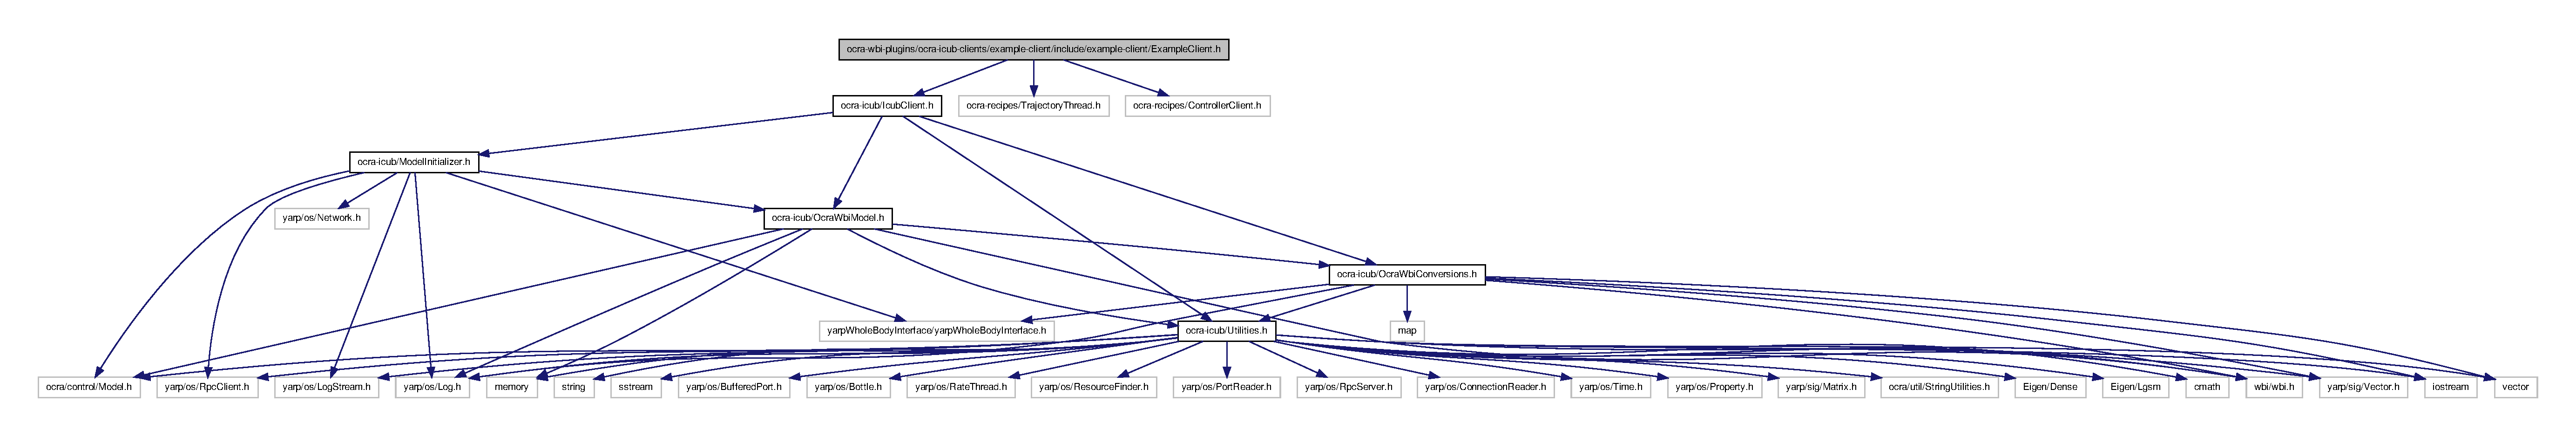
\includegraphics[width=350pt]{ExampleClient_8h__incl}
\end{center}
\end{figure}
\-This graph shows which files directly or indirectly include this file\-:
\nopagebreak
\begin{figure}[H]
\begin{center}
\leavevmode
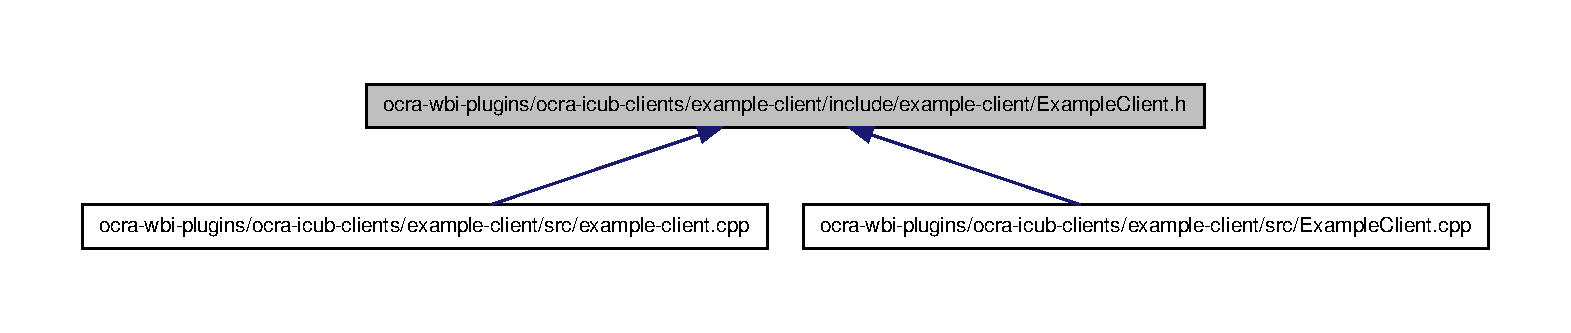
\includegraphics[width=350pt]{ExampleClient_8h__dep__incl}
\end{center}
\end{figure}
\subsection*{\-Classes}
\begin{DoxyCompactItemize}
\item 
class \hyperlink{classExampleClient}{\-Example\-Client}
\end{DoxyCompactItemize}

\hypertarget{example-client_8cpp}{\section{ocra-\/wbi-\/plugins/ocra-\/icub-\/clients/example-\/client/src/example-\/client.cpp \-File \-Reference}
\label{example-client_8cpp}\index{ocra-\/wbi-\/plugins/ocra-\/icub-\/clients/example-\/client/src/example-\/client.\-cpp@{ocra-\/wbi-\/plugins/ocra-\/icub-\/clients/example-\/client/src/example-\/client.\-cpp}}
}
{\ttfamily \#include $<$yarp/os/\-Resource\-Finder.\-h$>$}\*
{\ttfamily \#include $<$yarp/os/\-Network.\-h$>$}\*
{\ttfamily \#include $<$yarp/os/\-Log.\-h$>$}\*
{\ttfamily \#include $<$yarp/os/\-Log\-Stream.\-h$>$}\*
{\ttfamily \#include $<$yarp/os/\-Time.\-h$>$}\*
{\ttfamily \#include \char`\"{}example-\/client/\-Example\-Client.\-h\char`\"{}}\*
{\ttfamily \#include $<$ocra-\/icub/\-Icub\-Client.\-h$>$}\*
{\ttfamily \#include $<$ocra-\/recipes/\-Controller\-Client.\-h$>$}\*
{\ttfamily \#include $<$ocra-\/recipes/\-Client\-Manager.\-h$>$}\*
\-Include dependency graph for example-\/client.cpp\-:\nopagebreak
\begin{figure}[H]
\begin{center}
\leavevmode
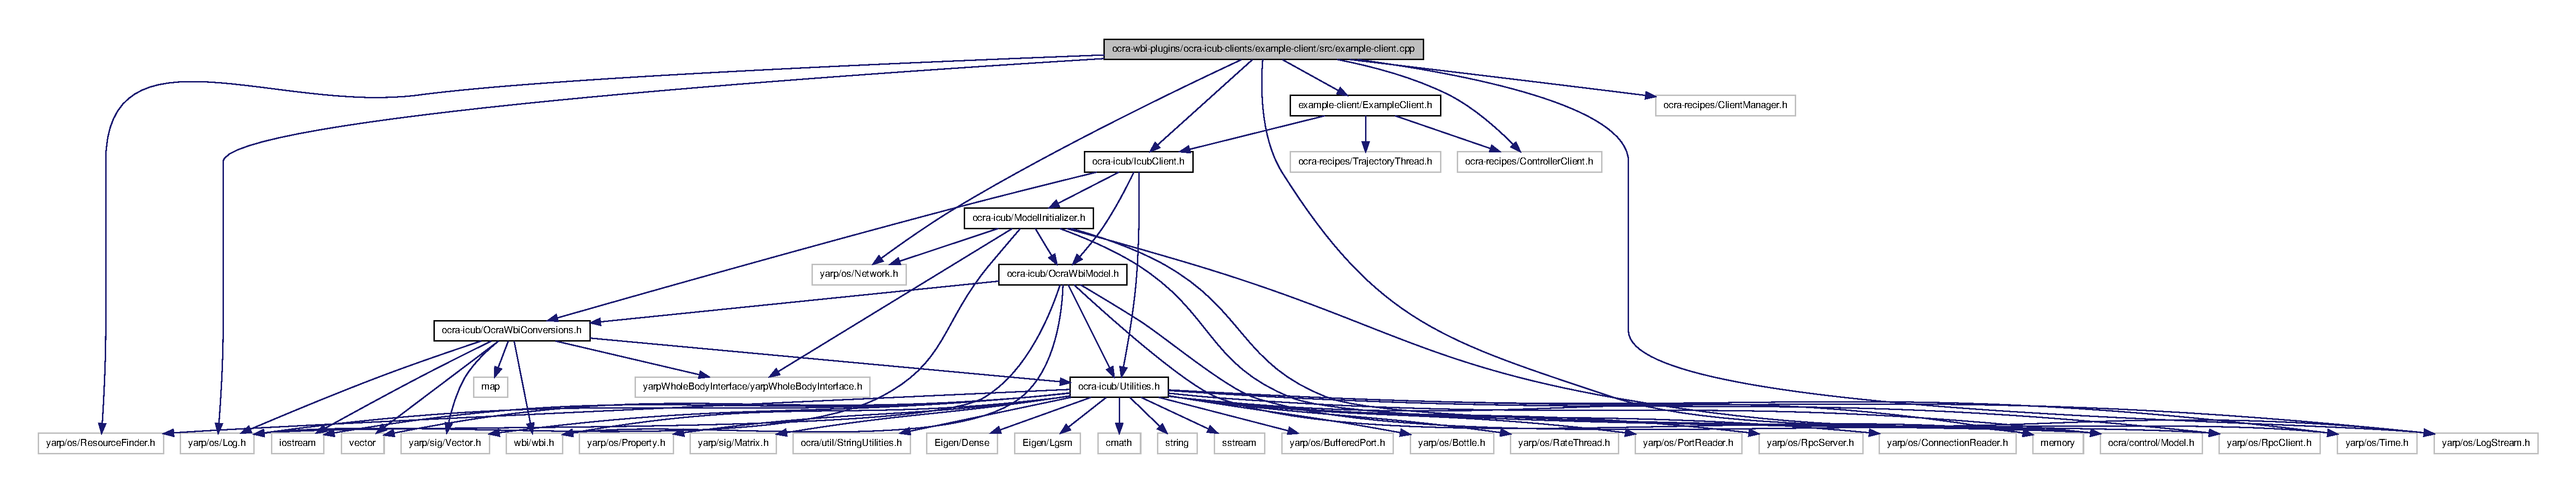
\includegraphics[width=350pt]{example-client_8cpp__incl}
\end{center}
\end{figure}
\subsection*{\-Functions}
\begin{DoxyCompactItemize}
\item 
int \hyperlink{example-client_8cpp_a0ddf1224851353fc92bfbff6f499fa97}{main} (int argc, char $\ast$argv\mbox{[}$\,$\mbox{]})
\end{DoxyCompactItemize}


\subsection{\-Detailed \-Description}
\begin{DoxyAuthor}{\-Author}
\mbox{[}\-Ryan \-Lober\mbox{]}(\href{http://www.ryanlober.com}{\tt http\-://www.\-ryanlober.\-com}) 

\mbox{[}\-Antoine \-Hoarau\mbox{]}(\href{http://ahoarau.github.io}{\tt http\-://ahoarau.\-github.\-io}) 
\end{DoxyAuthor}
\begin{DoxyDate}{\-Date}
\-Feb 2016 
\end{DoxyDate}
\begin{DoxyCopyright}{\-Copyright}
\-G\-N\-U \-General \-Public \-License. 
\end{DoxyCopyright}


\subsection{\-Function \-Documentation}
\hypertarget{example-client_8cpp_a0ddf1224851353fc92bfbff6f499fa97}{\index{example-\/client.\-cpp@{example-\/client.\-cpp}!main@{main}}
\index{main@{main}!example-client.cpp@{example-\/client.\-cpp}}
\subsubsection[{main}]{\setlength{\rightskip}{0pt plus 5cm}int {\bf main} (
\begin{DoxyParamCaption}
\item[{int}]{argc, }
\item[{char $\ast$}]{argv\mbox{[}$\,$\mbox{]}}
\end{DoxyParamCaption}
)}}\label{example-client_8cpp_a0ddf1224851353fc92bfbff6f499fa97}

\hypertarget{ExampleClient_8cpp}{\section{ocra-\/wbi-\/plugins/ocra-\/icub-\/clients/example-\/client/src/\-Example\-Client.cpp \-File \-Reference}
\label{ExampleClient_8cpp}\index{ocra-\/wbi-\/plugins/ocra-\/icub-\/clients/example-\/client/src/\-Example\-Client.\-cpp@{ocra-\/wbi-\/plugins/ocra-\/icub-\/clients/example-\/client/src/\-Example\-Client.\-cpp}}
}
{\ttfamily \#include \char`\"{}example-\/client/\-Example\-Client.\-h\char`\"{}}\*
\-Include dependency graph for \-Example\-Client.\-cpp\-:\nopagebreak
\begin{figure}[H]
\begin{center}
\leavevmode
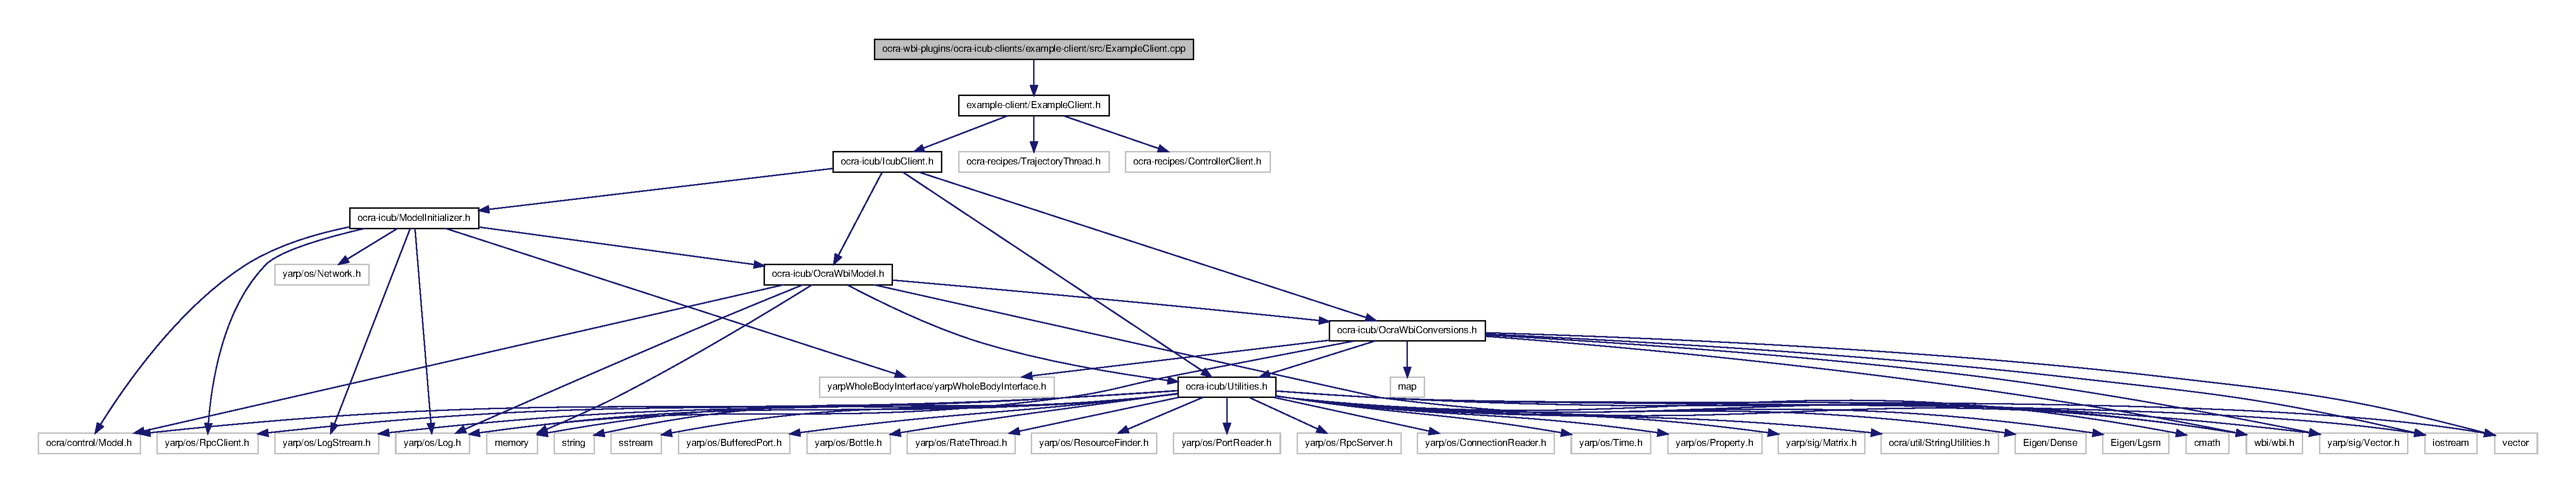
\includegraphics[width=350pt]{ExampleClient_8cpp__incl}
\end{center}
\end{figure}

\hypertarget{SittingDemoClient_8h}{\section{ocra-\/wbi-\/plugins/ocra-\/icub-\/clients/sitting-\/demo/include/sitting-\/demo/\-Sitting\-Demo\-Client.h \-File \-Reference}
\label{SittingDemoClient_8h}\index{ocra-\/wbi-\/plugins/ocra-\/icub-\/clients/sitting-\/demo/include/sitting-\/demo/\-Sitting\-Demo\-Client.\-h@{ocra-\/wbi-\/plugins/ocra-\/icub-\/clients/sitting-\/demo/include/sitting-\/demo/\-Sitting\-Demo\-Client.\-h}}
}
{\ttfamily \#include $<$ocra-\/icub/\-Icub\-Client.\-h$>$}\*
{\ttfamily \#include $<$ocra-\/recipes/\-Trajectory\-Thread.\-h$>$}\*
{\ttfamily \#include $<$ocra-\/recipes/\-Controller\-Client.\-h$>$}\*
\-Include dependency graph for \-Sitting\-Demo\-Client.\-h\-:\nopagebreak
\begin{figure}[H]
\begin{center}
\leavevmode
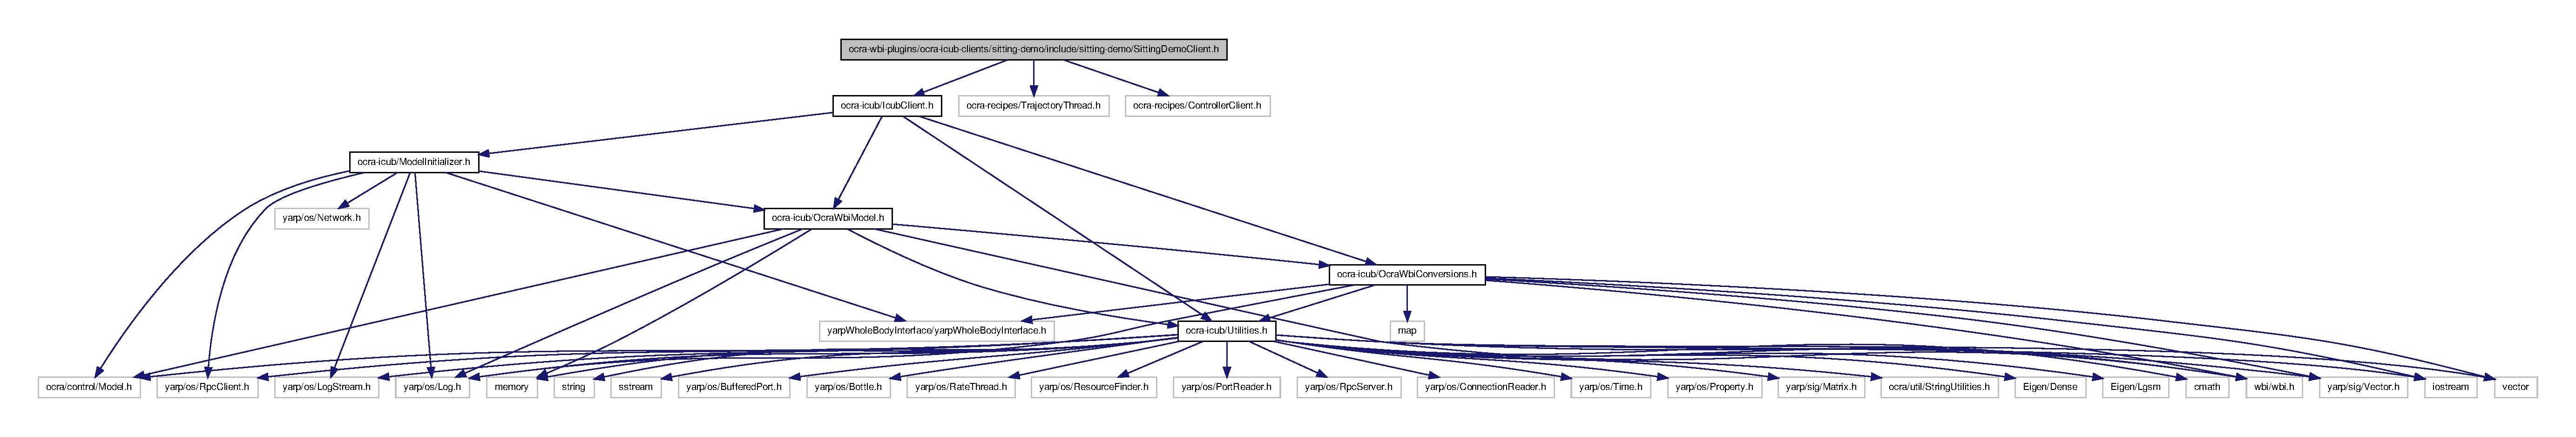
\includegraphics[width=350pt]{SittingDemoClient_8h__incl}
\end{center}
\end{figure}
\-This graph shows which files directly or indirectly include this file\-:\nopagebreak
\begin{figure}[H]
\begin{center}
\leavevmode
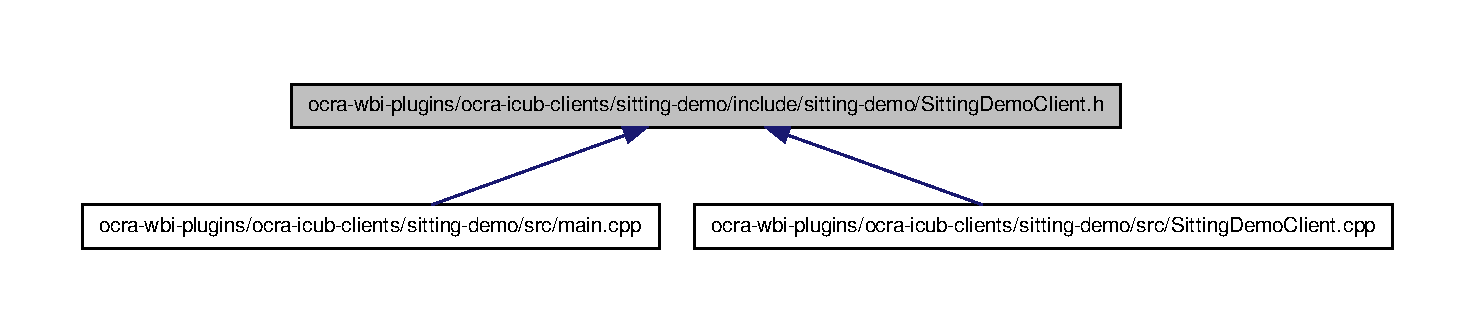
\includegraphics[width=350pt]{SittingDemoClient_8h__dep__incl}
\end{center}
\end{figure}
\subsection*{\-Classes}
\begin{DoxyCompactItemize}
\item 
class \hyperlink{classSittingDemoClient}{\-Sitting\-Demo\-Client}
\end{DoxyCompactItemize}

\hypertarget{SittingDemoClient_8cpp}{\section{ocra-\/wbi-\/plugins/ocra-\/icub-\/clients/sitting-\/demo/src/\-Sitting\-Demo\-Client.cpp \-File \-Reference}
\label{SittingDemoClient_8cpp}\index{ocra-\/wbi-\/plugins/ocra-\/icub-\/clients/sitting-\/demo/src/\-Sitting\-Demo\-Client.\-cpp@{ocra-\/wbi-\/plugins/ocra-\/icub-\/clients/sitting-\/demo/src/\-Sitting\-Demo\-Client.\-cpp}}
}
{\ttfamily \#include \char`\"{}sitting-\/demo/\-Sitting\-Demo\-Client.\-h\char`\"{}}\*
\-Include dependency graph for \-Sitting\-Demo\-Client.\-cpp\-:\nopagebreak
\begin{figure}[H]
\begin{center}
\leavevmode
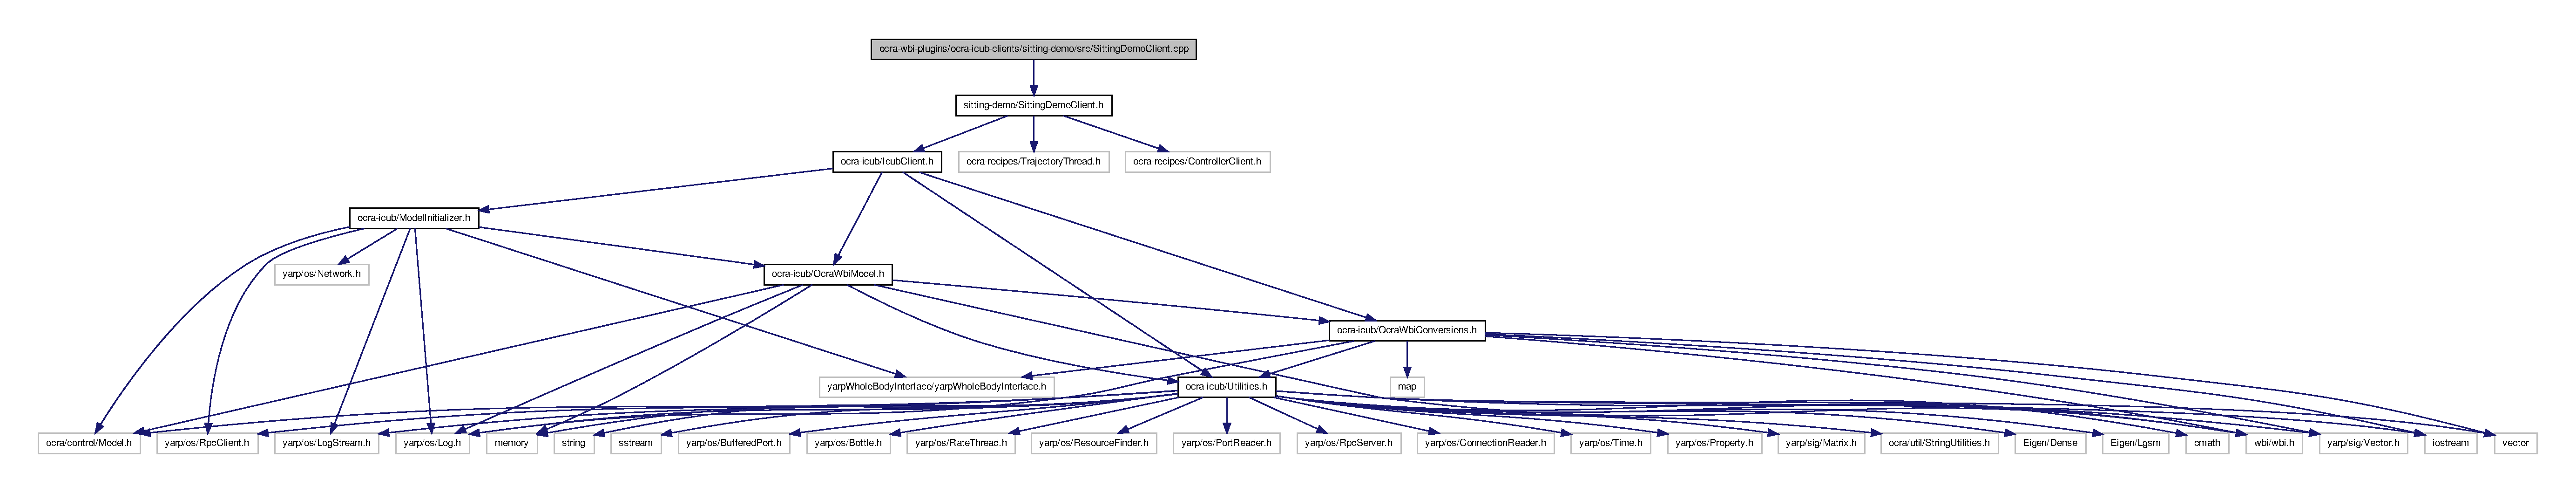
\includegraphics[width=350pt]{SittingDemoClient_8cpp__incl}
\end{center}
\end{figure}

\hypertarget{StandingDemoClient_8h}{\section{ocra-\/wbi-\/plugins/ocra-\/icub-\/clients/standing-\/demo/include/standing-\/demo/\-Standing\-Demo\-Client.h \-File \-Reference}
\label{StandingDemoClient_8h}\index{ocra-\/wbi-\/plugins/ocra-\/icub-\/clients/standing-\/demo/include/standing-\/demo/\-Standing\-Demo\-Client.\-h@{ocra-\/wbi-\/plugins/ocra-\/icub-\/clients/standing-\/demo/include/standing-\/demo/\-Standing\-Demo\-Client.\-h}}
}
{\ttfamily \#include $<$ocra-\/icub/\-Icub\-Client.\-h$>$}\*
{\ttfamily \#include $<$ocra-\/recipes/\-Trajectory\-Thread.\-h$>$}\*
{\ttfamily \#include $<$ocra-\/recipes/\-Controller\-Client.\-h$>$}\*
\-Include dependency graph for \-Standing\-Demo\-Client.\-h\-:
\nopagebreak
\begin{figure}[H]
\begin{center}
\leavevmode
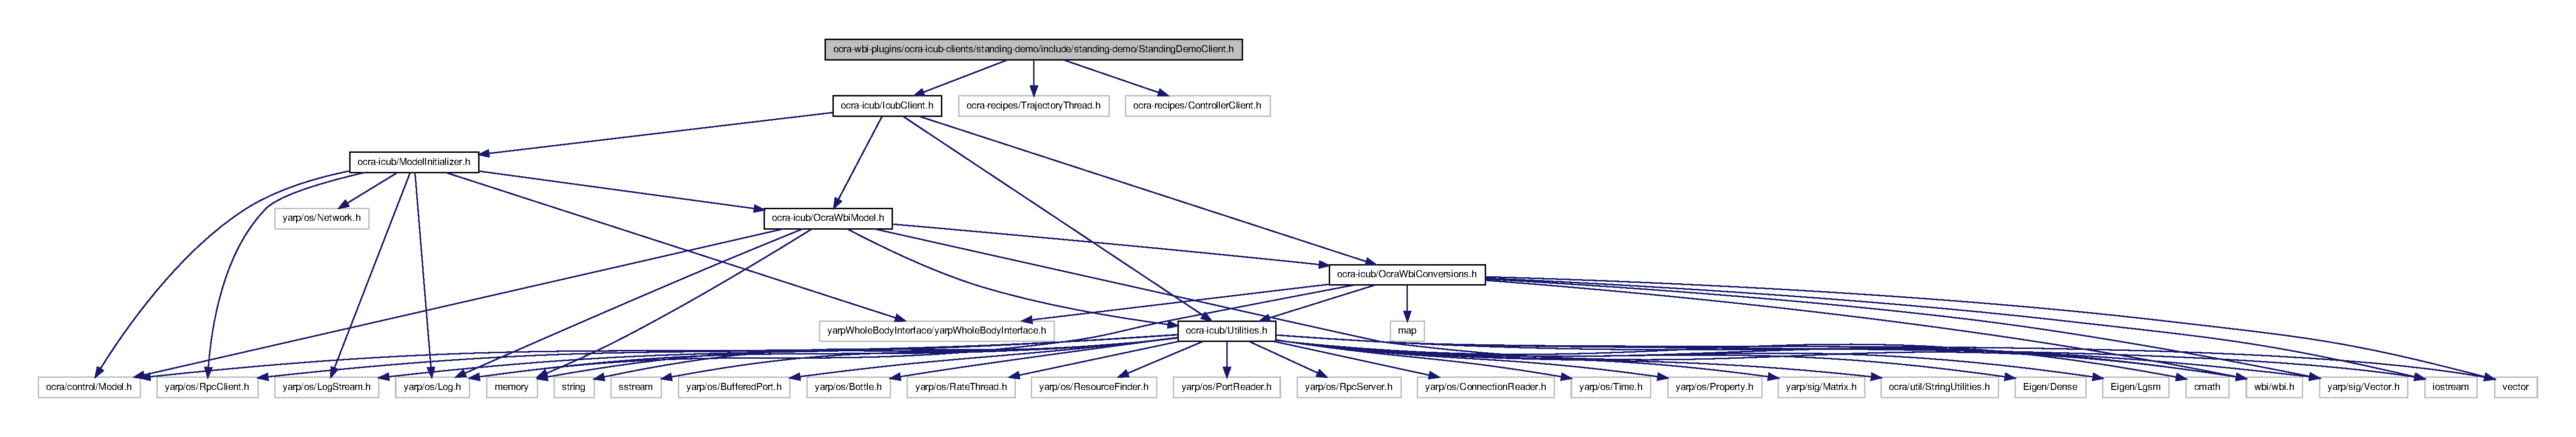
\includegraphics[width=350pt]{StandingDemoClient_8h__incl}
\end{center}
\end{figure}
\-This graph shows which files directly or indirectly include this file\-:
\nopagebreak
\begin{figure}[H]
\begin{center}
\leavevmode
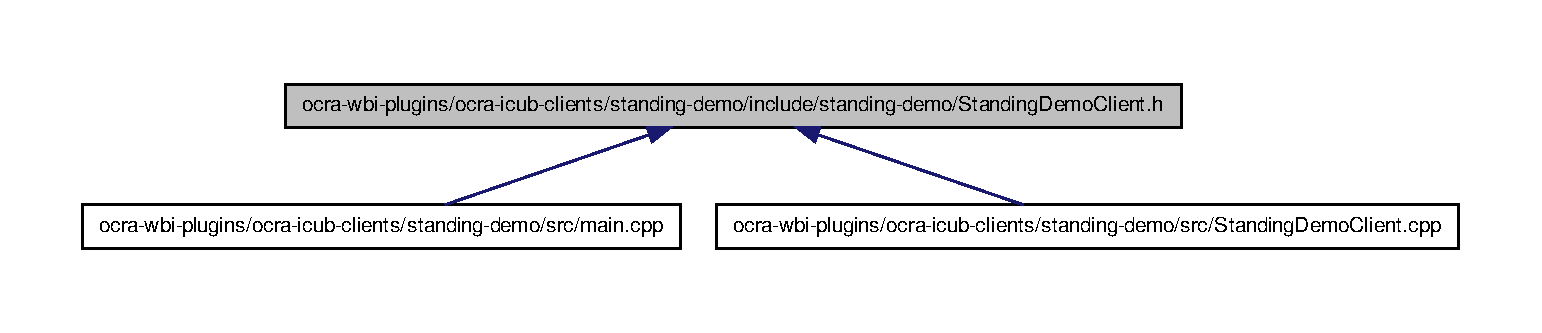
\includegraphics[width=350pt]{StandingDemoClient_8h__dep__incl}
\end{center}
\end{figure}
\subsection*{\-Classes}
\begin{DoxyCompactItemize}
\item 
class \hyperlink{classStandingDemoClient}{\-Standing\-Demo\-Client}
\end{DoxyCompactItemize}

\hypertarget{StandingDemoClient_8cpp}{\section{ocra-\/wbi-\/plugins/ocra-\/icub-\/clients/standing-\/demo/src/\-Standing\-Demo\-Client.cpp \-File \-Reference}
\label{StandingDemoClient_8cpp}\index{ocra-\/wbi-\/plugins/ocra-\/icub-\/clients/standing-\/demo/src/\-Standing\-Demo\-Client.\-cpp@{ocra-\/wbi-\/plugins/ocra-\/icub-\/clients/standing-\/demo/src/\-Standing\-Demo\-Client.\-cpp}}
}
{\ttfamily \#include \char`\"{}standing-\/demo/\-Standing\-Demo\-Client.\-h\char`\"{}}\*
\-Include dependency graph for \-Standing\-Demo\-Client.\-cpp\-:
\nopagebreak
\begin{figure}[H]
\begin{center}
\leavevmode
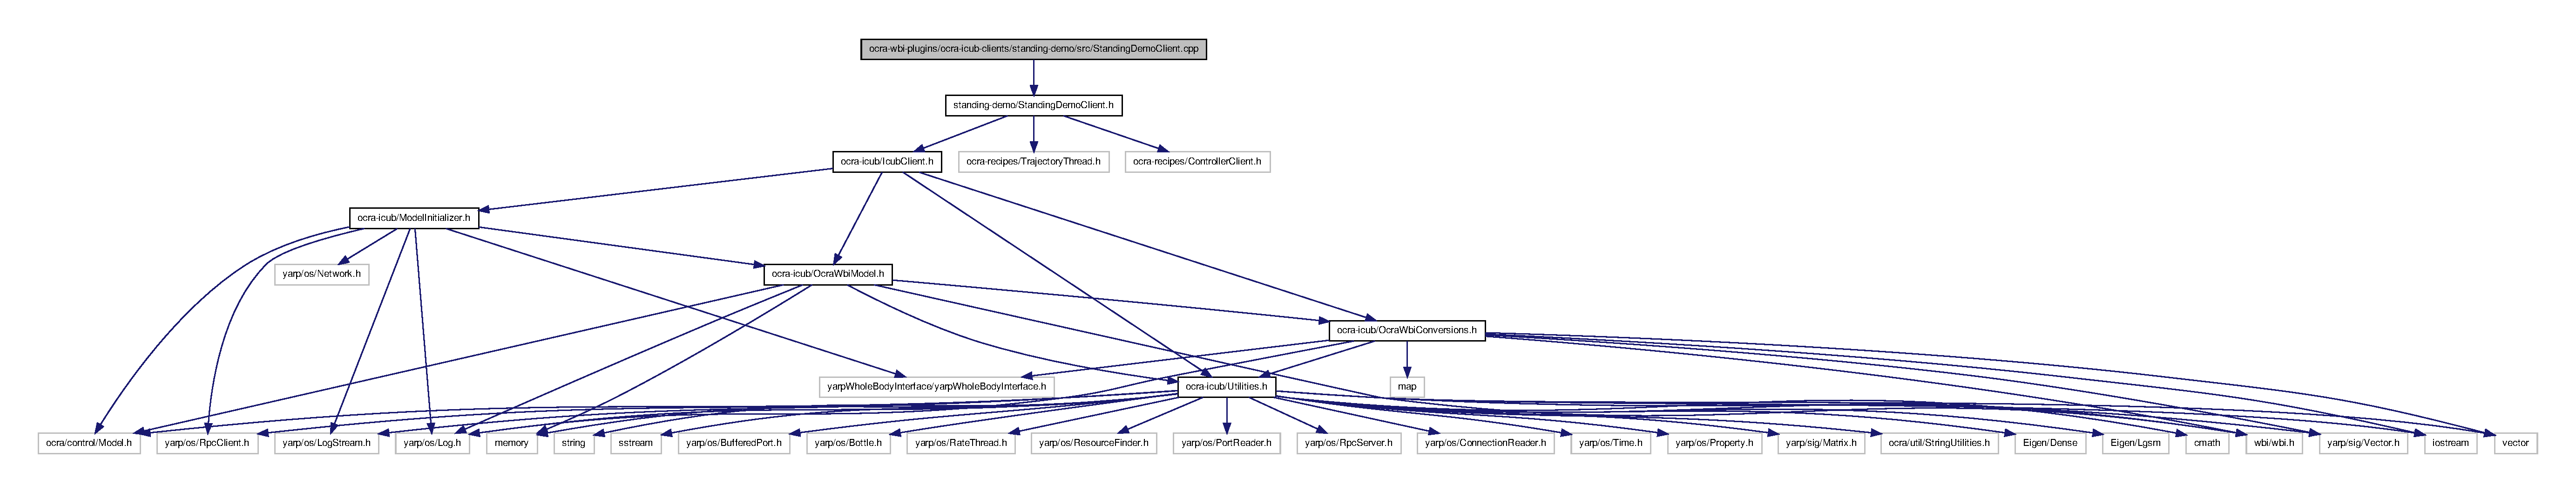
\includegraphics[width=350pt]{StandingDemoClient_8cpp__incl}
\end{center}
\end{figure}

\hypertarget{SteppingDemoClient_8h}{\section{ocra-\/wbi-\/plugins/ocra-\/icub-\/clients/stepping-\/demo/include/stepping-\/demo/\-Stepping\-Demo\-Client.h \-File \-Reference}
\label{SteppingDemoClient_8h}\index{ocra-\/wbi-\/plugins/ocra-\/icub-\/clients/stepping-\/demo/include/stepping-\/demo/\-Stepping\-Demo\-Client.\-h@{ocra-\/wbi-\/plugins/ocra-\/icub-\/clients/stepping-\/demo/include/stepping-\/demo/\-Stepping\-Demo\-Client.\-h}}
}
{\ttfamily \#include $<$ocra-\/icub/\-Icub\-Client.\-h$>$}\*
{\ttfamily \#include $<$ocra-\/recipes/\-Trajectory\-Thread.\-h$>$}\*
{\ttfamily \#include $<$ocra-\/recipes/\-Controller\-Client.\-h$>$}\*
{\ttfamily \#include $<$ocra/util/\-Errors\-Helper.\-h$>$}\*
\-Include dependency graph for \-Stepping\-Demo\-Client.\-h\-:
\nopagebreak
\begin{figure}[H]
\begin{center}
\leavevmode
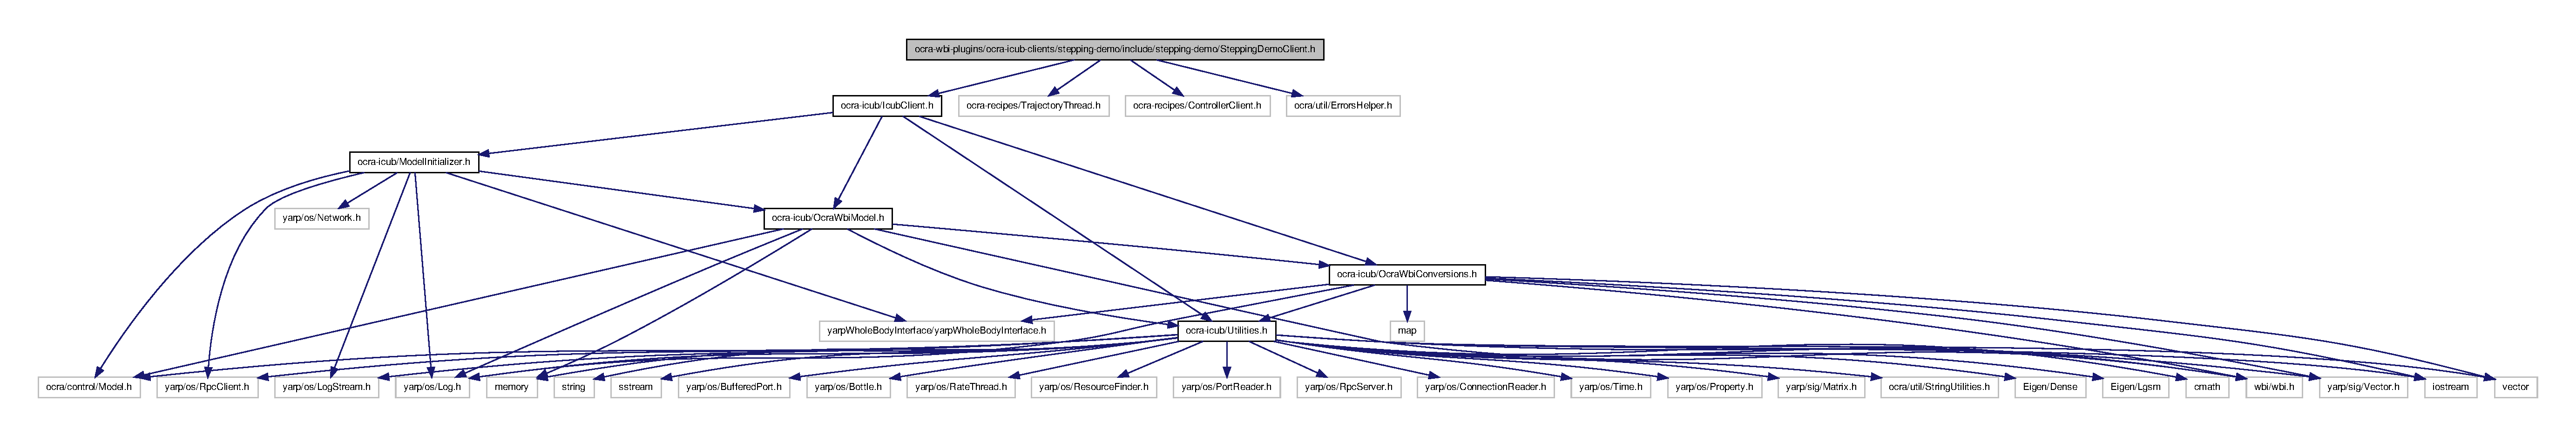
\includegraphics[width=350pt]{SteppingDemoClient_8h__incl}
\end{center}
\end{figure}
\-This graph shows which files directly or indirectly include this file\-:
\nopagebreak
\begin{figure}[H]
\begin{center}
\leavevmode
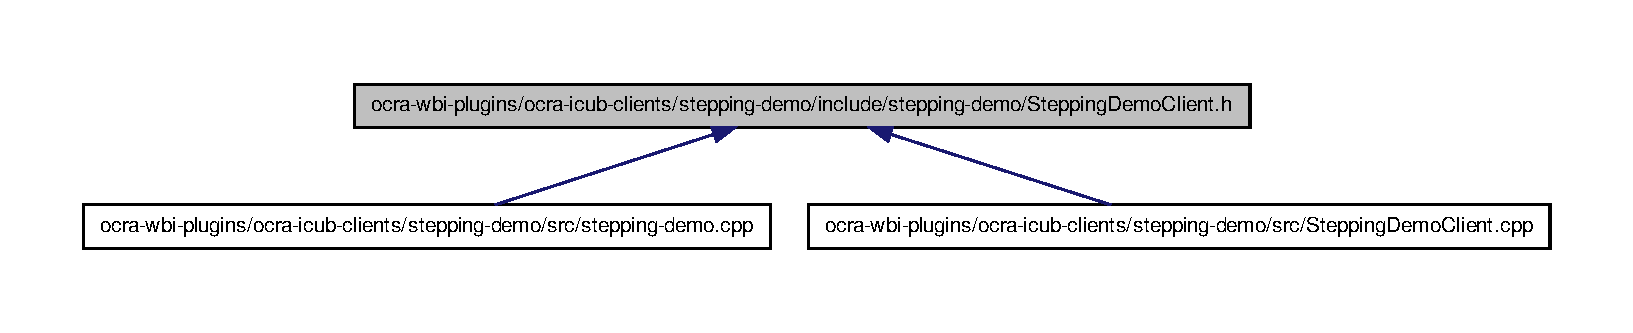
\includegraphics[width=350pt]{SteppingDemoClient_8h__dep__incl}
\end{center}
\end{figure}
\subsection*{\-Classes}
\begin{DoxyCompactItemize}
\item 
struct \hyperlink{structWalkingParams}{\-Walking\-Params}
\item 
class \hyperlink{classSteppingDemoClient}{\-Stepping\-Demo\-Client}
\end{DoxyCompactItemize}
\subsection*{\-Enumerations}
\begin{DoxyCompactItemize}
\item 
enum \hyperlink{SteppingDemoClient_8h_ac0c3848a609566394821d9826e0fdd5b}{\-C\-O\-M\-\_\-\-S\-U\-P\-P\-O\-R\-T\-\_\-\-P\-O\-S\-I\-T\-I\-O\-N} \{ \hyperlink{SteppingDemoClient_8h_ac0c3848a609566394821d9826e0fdd5ba07cd79ee915be269a43f655f31cd3ccf}{\-L\-E\-F\-T\-\_\-\-F\-O\-O\-T\-\_\-\-X\-Y}, 
\hyperlink{SteppingDemoClient_8h_ac0c3848a609566394821d9826e0fdd5ba273605381ab0231d2abb4a8096faabfd}{\-R\-I\-G\-H\-T\-\_\-\-F\-O\-O\-T\-\_\-\-X\-Y}, 
\hyperlink{SteppingDemoClient_8h_ac0c3848a609566394821d9826e0fdd5bad32a9ea5bb598218529abf1a5b9b50cf}{\-C\-E\-N\-T\-E\-R\-E\-D\-\_\-\-B\-E\-T\-W\-E\-E\-N\-\_\-\-F\-E\-E\-T\-\_\-\-X\-Y}
 \}
\item 
enum \hyperlink{SteppingDemoClient_8h_af2a8507bf21c3ce9b0e67a23381251c6}{\-C\-O\-N\-T\-R\-O\-L\-\_\-\-P\-H\-A\-S\-E} \{ \hyperlink{SteppingDemoClient_8h_af2a8507bf21c3ce9b0e67a23381251c6afe7fc4a2f5d6778bbb96f412be37d63c}{\-M\-O\-V\-E\-\_\-\-T\-O\-\_\-\-L\-E\-F\-T\-\_\-\-S\-U\-P\-P\-O\-R\-T}, 
\hyperlink{SteppingDemoClient_8h_af2a8507bf21c3ce9b0e67a23381251c6a3b4335037acf972dd5d60348ca20d394}{\-M\-O\-V\-E\-\_\-\-T\-O\-\_\-\-R\-I\-G\-H\-T\-\_\-\-S\-U\-P\-P\-O\-R\-T}, 
\hyperlink{SteppingDemoClient_8h_af2a8507bf21c3ce9b0e67a23381251c6a362d8557e44bcc19f6b4d9096bb54401}{\-M\-O\-V\-E\-\_\-\-T\-O\-\_\-\-D\-O\-U\-B\-L\-E\-\_\-\-S\-U\-P\-P\-O\-R\-T}, 
\hyperlink{SteppingDemoClient_8h_af2a8507bf21c3ce9b0e67a23381251c6a4ff6c6ae9503ea4bca745c7d7819523e}{\-S\-T\-E\-P\-\_\-\-F\-O\-R\-W\-A\-R\-D}
 \}
\item 
enum \hyperlink{SteppingDemoClient_8h_ab0673d7f17cdd57b8fa124abb330287f}{\-F\-O\-O\-T\-\_\-\-C\-O\-N\-T\-A\-C\-T\-S} \{ \hyperlink{SteppingDemoClient_8h_ab0673d7f17cdd57b8fa124abb330287fa7760daad9db1ede8c57b06189deca9f3}{\-L\-E\-F\-T\-\_\-\-F\-O\-O\-T}, 
\hyperlink{SteppingDemoClient_8h_ab0673d7f17cdd57b8fa124abb330287face119c66af60ac0781b137aa87d7be62}{\-R\-I\-G\-H\-T\-\_\-\-F\-O\-O\-T}
 \}
\item 
enum \hyperlink{SteppingDemoClient_8h_abd6d177d63e98aa1b4ed4b8329e2a379}{\-M\-O\-T\-I\-O\-N\-\_\-\-T\-Y\-P\-E} \{ \hyperlink{SteppingDemoClient_8h_abd6d177d63e98aa1b4ed4b8329e2a379a55b57dce74f14a62104ae66e62789eb3}{\-L\-E\-F\-T\-\_\-\-T\-O\-\_\-\-R\-I\-G\-H\-T}, 
\hyperlink{SteppingDemoClient_8h_abd6d177d63e98aa1b4ed4b8329e2a379ada7017955bb1db9f0954017358028fa6}{\-S\-T\-A\-T\-I\-C\-\_\-\-W\-A\-L\-K\-I\-N\-G}
 \}
\end{DoxyCompactItemize}


\subsection{\-Enumeration \-Type \-Documentation}
\hypertarget{SteppingDemoClient_8h_ac0c3848a609566394821d9826e0fdd5b}{\index{\-Stepping\-Demo\-Client.\-h@{\-Stepping\-Demo\-Client.\-h}!\-C\-O\-M\-\_\-\-S\-U\-P\-P\-O\-R\-T\-\_\-\-P\-O\-S\-I\-T\-I\-O\-N@{\-C\-O\-M\-\_\-\-S\-U\-P\-P\-O\-R\-T\-\_\-\-P\-O\-S\-I\-T\-I\-O\-N}}
\index{\-C\-O\-M\-\_\-\-S\-U\-P\-P\-O\-R\-T\-\_\-\-P\-O\-S\-I\-T\-I\-O\-N@{\-C\-O\-M\-\_\-\-S\-U\-P\-P\-O\-R\-T\-\_\-\-P\-O\-S\-I\-T\-I\-O\-N}!SteppingDemoClient.h@{\-Stepping\-Demo\-Client.\-h}}
\subsubsection[{\-C\-O\-M\-\_\-\-S\-U\-P\-P\-O\-R\-T\-\_\-\-P\-O\-S\-I\-T\-I\-O\-N}]{\setlength{\rightskip}{0pt plus 5cm}enum {\bf \-C\-O\-M\-\_\-\-S\-U\-P\-P\-O\-R\-T\-\_\-\-P\-O\-S\-I\-T\-I\-O\-N}}}\label{SteppingDemoClient_8h_ac0c3848a609566394821d9826e0fdd5b}
\begin{Desc}
\item[\-Enumerator\-: ]\par
\begin{description}
\index{\-L\-E\-F\-T\-\_\-\-F\-O\-O\-T\-\_\-\-X\-Y@{\-L\-E\-F\-T\-\_\-\-F\-O\-O\-T\-\_\-\-X\-Y}!\-Stepping\-Demo\-Client.\-h@{\-Stepping\-Demo\-Client.\-h}}\index{\-Stepping\-Demo\-Client.\-h@{\-Stepping\-Demo\-Client.\-h}!\-L\-E\-F\-T\-\_\-\-F\-O\-O\-T\-\_\-\-X\-Y@{\-L\-E\-F\-T\-\_\-\-F\-O\-O\-T\-\_\-\-X\-Y}}\item[{\em 
\hypertarget{SteppingDemoClient_8h_ac0c3848a609566394821d9826e0fdd5ba07cd79ee915be269a43f655f31cd3ccf}{\-L\-E\-F\-T\-\_\-\-F\-O\-O\-T\-\_\-\-X\-Y}\label{SteppingDemoClient_8h_ac0c3848a609566394821d9826e0fdd5ba07cd79ee915be269a43f655f31cd3ccf}
}]\index{\-R\-I\-G\-H\-T\-\_\-\-F\-O\-O\-T\-\_\-\-X\-Y@{\-R\-I\-G\-H\-T\-\_\-\-F\-O\-O\-T\-\_\-\-X\-Y}!\-Stepping\-Demo\-Client.\-h@{\-Stepping\-Demo\-Client.\-h}}\index{\-Stepping\-Demo\-Client.\-h@{\-Stepping\-Demo\-Client.\-h}!\-R\-I\-G\-H\-T\-\_\-\-F\-O\-O\-T\-\_\-\-X\-Y@{\-R\-I\-G\-H\-T\-\_\-\-F\-O\-O\-T\-\_\-\-X\-Y}}\item[{\em 
\hypertarget{SteppingDemoClient_8h_ac0c3848a609566394821d9826e0fdd5ba273605381ab0231d2abb4a8096faabfd}{\-R\-I\-G\-H\-T\-\_\-\-F\-O\-O\-T\-\_\-\-X\-Y}\label{SteppingDemoClient_8h_ac0c3848a609566394821d9826e0fdd5ba273605381ab0231d2abb4a8096faabfd}
}]\index{\-C\-E\-N\-T\-E\-R\-E\-D\-\_\-\-B\-E\-T\-W\-E\-E\-N\-\_\-\-F\-E\-E\-T\-\_\-\-X\-Y@{\-C\-E\-N\-T\-E\-R\-E\-D\-\_\-\-B\-E\-T\-W\-E\-E\-N\-\_\-\-F\-E\-E\-T\-\_\-\-X\-Y}!\-Stepping\-Demo\-Client.\-h@{\-Stepping\-Demo\-Client.\-h}}\index{\-Stepping\-Demo\-Client.\-h@{\-Stepping\-Demo\-Client.\-h}!\-C\-E\-N\-T\-E\-R\-E\-D\-\_\-\-B\-E\-T\-W\-E\-E\-N\-\_\-\-F\-E\-E\-T\-\_\-\-X\-Y@{\-C\-E\-N\-T\-E\-R\-E\-D\-\_\-\-B\-E\-T\-W\-E\-E\-N\-\_\-\-F\-E\-E\-T\-\_\-\-X\-Y}}\item[{\em 
\hypertarget{SteppingDemoClient_8h_ac0c3848a609566394821d9826e0fdd5bad32a9ea5bb598218529abf1a5b9b50cf}{\-C\-E\-N\-T\-E\-R\-E\-D\-\_\-\-B\-E\-T\-W\-E\-E\-N\-\_\-\-F\-E\-E\-T\-\_\-\-X\-Y}\label{SteppingDemoClient_8h_ac0c3848a609566394821d9826e0fdd5bad32a9ea5bb598218529abf1a5b9b50cf}
}]\end{description}
\end{Desc}

\hypertarget{SteppingDemoClient_8h_af2a8507bf21c3ce9b0e67a23381251c6}{\index{\-Stepping\-Demo\-Client.\-h@{\-Stepping\-Demo\-Client.\-h}!\-C\-O\-N\-T\-R\-O\-L\-\_\-\-P\-H\-A\-S\-E@{\-C\-O\-N\-T\-R\-O\-L\-\_\-\-P\-H\-A\-S\-E}}
\index{\-C\-O\-N\-T\-R\-O\-L\-\_\-\-P\-H\-A\-S\-E@{\-C\-O\-N\-T\-R\-O\-L\-\_\-\-P\-H\-A\-S\-E}!SteppingDemoClient.h@{\-Stepping\-Demo\-Client.\-h}}
\subsubsection[{\-C\-O\-N\-T\-R\-O\-L\-\_\-\-P\-H\-A\-S\-E}]{\setlength{\rightskip}{0pt plus 5cm}enum {\bf \-C\-O\-N\-T\-R\-O\-L\-\_\-\-P\-H\-A\-S\-E}}}\label{SteppingDemoClient_8h_af2a8507bf21c3ce9b0e67a23381251c6}
\begin{Desc}
\item[\-Enumerator\-: ]\par
\begin{description}
\index{\-M\-O\-V\-E\-\_\-\-T\-O\-\_\-\-L\-E\-F\-T\-\_\-\-S\-U\-P\-P\-O\-R\-T@{\-M\-O\-V\-E\-\_\-\-T\-O\-\_\-\-L\-E\-F\-T\-\_\-\-S\-U\-P\-P\-O\-R\-T}!\-Stepping\-Demo\-Client.\-h@{\-Stepping\-Demo\-Client.\-h}}\index{\-Stepping\-Demo\-Client.\-h@{\-Stepping\-Demo\-Client.\-h}!\-M\-O\-V\-E\-\_\-\-T\-O\-\_\-\-L\-E\-F\-T\-\_\-\-S\-U\-P\-P\-O\-R\-T@{\-M\-O\-V\-E\-\_\-\-T\-O\-\_\-\-L\-E\-F\-T\-\_\-\-S\-U\-P\-P\-O\-R\-T}}\item[{\em 
\hypertarget{SteppingDemoClient_8h_af2a8507bf21c3ce9b0e67a23381251c6afe7fc4a2f5d6778bbb96f412be37d63c}{\-M\-O\-V\-E\-\_\-\-T\-O\-\_\-\-L\-E\-F\-T\-\_\-\-S\-U\-P\-P\-O\-R\-T}\label{SteppingDemoClient_8h_af2a8507bf21c3ce9b0e67a23381251c6afe7fc4a2f5d6778bbb96f412be37d63c}
}]\index{\-M\-O\-V\-E\-\_\-\-T\-O\-\_\-\-R\-I\-G\-H\-T\-\_\-\-S\-U\-P\-P\-O\-R\-T@{\-M\-O\-V\-E\-\_\-\-T\-O\-\_\-\-R\-I\-G\-H\-T\-\_\-\-S\-U\-P\-P\-O\-R\-T}!\-Stepping\-Demo\-Client.\-h@{\-Stepping\-Demo\-Client.\-h}}\index{\-Stepping\-Demo\-Client.\-h@{\-Stepping\-Demo\-Client.\-h}!\-M\-O\-V\-E\-\_\-\-T\-O\-\_\-\-R\-I\-G\-H\-T\-\_\-\-S\-U\-P\-P\-O\-R\-T@{\-M\-O\-V\-E\-\_\-\-T\-O\-\_\-\-R\-I\-G\-H\-T\-\_\-\-S\-U\-P\-P\-O\-R\-T}}\item[{\em 
\hypertarget{SteppingDemoClient_8h_af2a8507bf21c3ce9b0e67a23381251c6a3b4335037acf972dd5d60348ca20d394}{\-M\-O\-V\-E\-\_\-\-T\-O\-\_\-\-R\-I\-G\-H\-T\-\_\-\-S\-U\-P\-P\-O\-R\-T}\label{SteppingDemoClient_8h_af2a8507bf21c3ce9b0e67a23381251c6a3b4335037acf972dd5d60348ca20d394}
}]\index{\-M\-O\-V\-E\-\_\-\-T\-O\-\_\-\-D\-O\-U\-B\-L\-E\-\_\-\-S\-U\-P\-P\-O\-R\-T@{\-M\-O\-V\-E\-\_\-\-T\-O\-\_\-\-D\-O\-U\-B\-L\-E\-\_\-\-S\-U\-P\-P\-O\-R\-T}!\-Stepping\-Demo\-Client.\-h@{\-Stepping\-Demo\-Client.\-h}}\index{\-Stepping\-Demo\-Client.\-h@{\-Stepping\-Demo\-Client.\-h}!\-M\-O\-V\-E\-\_\-\-T\-O\-\_\-\-D\-O\-U\-B\-L\-E\-\_\-\-S\-U\-P\-P\-O\-R\-T@{\-M\-O\-V\-E\-\_\-\-T\-O\-\_\-\-D\-O\-U\-B\-L\-E\-\_\-\-S\-U\-P\-P\-O\-R\-T}}\item[{\em 
\hypertarget{SteppingDemoClient_8h_af2a8507bf21c3ce9b0e67a23381251c6a362d8557e44bcc19f6b4d9096bb54401}{\-M\-O\-V\-E\-\_\-\-T\-O\-\_\-\-D\-O\-U\-B\-L\-E\-\_\-\-S\-U\-P\-P\-O\-R\-T}\label{SteppingDemoClient_8h_af2a8507bf21c3ce9b0e67a23381251c6a362d8557e44bcc19f6b4d9096bb54401}
}]\index{\-S\-T\-E\-P\-\_\-\-F\-O\-R\-W\-A\-R\-D@{\-S\-T\-E\-P\-\_\-\-F\-O\-R\-W\-A\-R\-D}!\-Stepping\-Demo\-Client.\-h@{\-Stepping\-Demo\-Client.\-h}}\index{\-Stepping\-Demo\-Client.\-h@{\-Stepping\-Demo\-Client.\-h}!\-S\-T\-E\-P\-\_\-\-F\-O\-R\-W\-A\-R\-D@{\-S\-T\-E\-P\-\_\-\-F\-O\-R\-W\-A\-R\-D}}\item[{\em 
\hypertarget{SteppingDemoClient_8h_af2a8507bf21c3ce9b0e67a23381251c6a4ff6c6ae9503ea4bca745c7d7819523e}{\-S\-T\-E\-P\-\_\-\-F\-O\-R\-W\-A\-R\-D}\label{SteppingDemoClient_8h_af2a8507bf21c3ce9b0e67a23381251c6a4ff6c6ae9503ea4bca745c7d7819523e}
}]\end{description}
\end{Desc}

\hypertarget{SteppingDemoClient_8h_ab0673d7f17cdd57b8fa124abb330287f}{\index{\-Stepping\-Demo\-Client.\-h@{\-Stepping\-Demo\-Client.\-h}!\-F\-O\-O\-T\-\_\-\-C\-O\-N\-T\-A\-C\-T\-S@{\-F\-O\-O\-T\-\_\-\-C\-O\-N\-T\-A\-C\-T\-S}}
\index{\-F\-O\-O\-T\-\_\-\-C\-O\-N\-T\-A\-C\-T\-S@{\-F\-O\-O\-T\-\_\-\-C\-O\-N\-T\-A\-C\-T\-S}!SteppingDemoClient.h@{\-Stepping\-Demo\-Client.\-h}}
\subsubsection[{\-F\-O\-O\-T\-\_\-\-C\-O\-N\-T\-A\-C\-T\-S}]{\setlength{\rightskip}{0pt plus 5cm}enum {\bf \-F\-O\-O\-T\-\_\-\-C\-O\-N\-T\-A\-C\-T\-S}}}\label{SteppingDemoClient_8h_ab0673d7f17cdd57b8fa124abb330287f}
\begin{Desc}
\item[\-Enumerator\-: ]\par
\begin{description}
\index{\-L\-E\-F\-T\-\_\-\-F\-O\-O\-T@{\-L\-E\-F\-T\-\_\-\-F\-O\-O\-T}!\-Stepping\-Demo\-Client.\-h@{\-Stepping\-Demo\-Client.\-h}}\index{\-Stepping\-Demo\-Client.\-h@{\-Stepping\-Demo\-Client.\-h}!\-L\-E\-F\-T\-\_\-\-F\-O\-O\-T@{\-L\-E\-F\-T\-\_\-\-F\-O\-O\-T}}\item[{\em 
\hypertarget{SteppingDemoClient_8h_ab0673d7f17cdd57b8fa124abb330287fa7760daad9db1ede8c57b06189deca9f3}{\-L\-E\-F\-T\-\_\-\-F\-O\-O\-T}\label{SteppingDemoClient_8h_ab0673d7f17cdd57b8fa124abb330287fa7760daad9db1ede8c57b06189deca9f3}
}]\index{\-R\-I\-G\-H\-T\-\_\-\-F\-O\-O\-T@{\-R\-I\-G\-H\-T\-\_\-\-F\-O\-O\-T}!\-Stepping\-Demo\-Client.\-h@{\-Stepping\-Demo\-Client.\-h}}\index{\-Stepping\-Demo\-Client.\-h@{\-Stepping\-Demo\-Client.\-h}!\-R\-I\-G\-H\-T\-\_\-\-F\-O\-O\-T@{\-R\-I\-G\-H\-T\-\_\-\-F\-O\-O\-T}}\item[{\em 
\hypertarget{SteppingDemoClient_8h_ab0673d7f17cdd57b8fa124abb330287face119c66af60ac0781b137aa87d7be62}{\-R\-I\-G\-H\-T\-\_\-\-F\-O\-O\-T}\label{SteppingDemoClient_8h_ab0673d7f17cdd57b8fa124abb330287face119c66af60ac0781b137aa87d7be62}
}]\end{description}
\end{Desc}

\hypertarget{SteppingDemoClient_8h_abd6d177d63e98aa1b4ed4b8329e2a379}{\index{\-Stepping\-Demo\-Client.\-h@{\-Stepping\-Demo\-Client.\-h}!\-M\-O\-T\-I\-O\-N\-\_\-\-T\-Y\-P\-E@{\-M\-O\-T\-I\-O\-N\-\_\-\-T\-Y\-P\-E}}
\index{\-M\-O\-T\-I\-O\-N\-\_\-\-T\-Y\-P\-E@{\-M\-O\-T\-I\-O\-N\-\_\-\-T\-Y\-P\-E}!SteppingDemoClient.h@{\-Stepping\-Demo\-Client.\-h}}
\subsubsection[{\-M\-O\-T\-I\-O\-N\-\_\-\-T\-Y\-P\-E}]{\setlength{\rightskip}{0pt plus 5cm}enum {\bf \-M\-O\-T\-I\-O\-N\-\_\-\-T\-Y\-P\-E}}}\label{SteppingDemoClient_8h_abd6d177d63e98aa1b4ed4b8329e2a379}
\begin{Desc}
\item[\-Enumerator\-: ]\par
\begin{description}
\index{\-L\-E\-F\-T\-\_\-\-T\-O\-\_\-\-R\-I\-G\-H\-T@{\-L\-E\-F\-T\-\_\-\-T\-O\-\_\-\-R\-I\-G\-H\-T}!\-Stepping\-Demo\-Client.\-h@{\-Stepping\-Demo\-Client.\-h}}\index{\-Stepping\-Demo\-Client.\-h@{\-Stepping\-Demo\-Client.\-h}!\-L\-E\-F\-T\-\_\-\-T\-O\-\_\-\-R\-I\-G\-H\-T@{\-L\-E\-F\-T\-\_\-\-T\-O\-\_\-\-R\-I\-G\-H\-T}}\item[{\em 
\hypertarget{SteppingDemoClient_8h_abd6d177d63e98aa1b4ed4b8329e2a379a55b57dce74f14a62104ae66e62789eb3}{\-L\-E\-F\-T\-\_\-\-T\-O\-\_\-\-R\-I\-G\-H\-T}\label{SteppingDemoClient_8h_abd6d177d63e98aa1b4ed4b8329e2a379a55b57dce74f14a62104ae66e62789eb3}
}]\index{\-S\-T\-A\-T\-I\-C\-\_\-\-W\-A\-L\-K\-I\-N\-G@{\-S\-T\-A\-T\-I\-C\-\_\-\-W\-A\-L\-K\-I\-N\-G}!\-Stepping\-Demo\-Client.\-h@{\-Stepping\-Demo\-Client.\-h}}\index{\-Stepping\-Demo\-Client.\-h@{\-Stepping\-Demo\-Client.\-h}!\-S\-T\-A\-T\-I\-C\-\_\-\-W\-A\-L\-K\-I\-N\-G@{\-S\-T\-A\-T\-I\-C\-\_\-\-W\-A\-L\-K\-I\-N\-G}}\item[{\em 
\hypertarget{SteppingDemoClient_8h_abd6d177d63e98aa1b4ed4b8329e2a379ada7017955bb1db9f0954017358028fa6}{\-S\-T\-A\-T\-I\-C\-\_\-\-W\-A\-L\-K\-I\-N\-G}\label{SteppingDemoClient_8h_abd6d177d63e98aa1b4ed4b8329e2a379ada7017955bb1db9f0954017358028fa6}
}]\end{description}
\end{Desc}


\hypertarget{stepping-demo_8cpp}{\section{ocra-\/wbi-\/plugins/ocra-\/icub-\/clients/stepping-\/demo/src/stepping-\/demo.cpp \-File \-Reference}
\label{stepping-demo_8cpp}\index{ocra-\/wbi-\/plugins/ocra-\/icub-\/clients/stepping-\/demo/src/stepping-\/demo.\-cpp@{ocra-\/wbi-\/plugins/ocra-\/icub-\/clients/stepping-\/demo/src/stepping-\/demo.\-cpp}}
}
{\ttfamily \#include $<$yarp/os/\-Resource\-Finder.\-h$>$}\*
{\ttfamily \#include $<$yarp/os/\-Network.\-h$>$}\*
{\ttfamily \#include $<$yarp/os/\-Log.\-h$>$}\*
{\ttfamily \#include $<$yarp/os/\-Log\-Stream.\-h$>$}\*
{\ttfamily \#include $<$yarp/os/\-Time.\-h$>$}\*
{\ttfamily \#include \char`\"{}stepping-\/demo/\-Stepping\-Demo\-Client.\-h\char`\"{}}\*
{\ttfamily \#include $<$ocra-\/icub/\-Icub\-Client.\-h$>$}\*
{\ttfamily \#include $<$ocra-\/recipes/\-Controller\-Client.\-h$>$}\*
{\ttfamily \#include $<$ocra-\/recipes/\-Client\-Manager.\-h$>$}\*
\-Include dependency graph for stepping-\/demo.cpp\-:\nopagebreak
\begin{figure}[H]
\begin{center}
\leavevmode
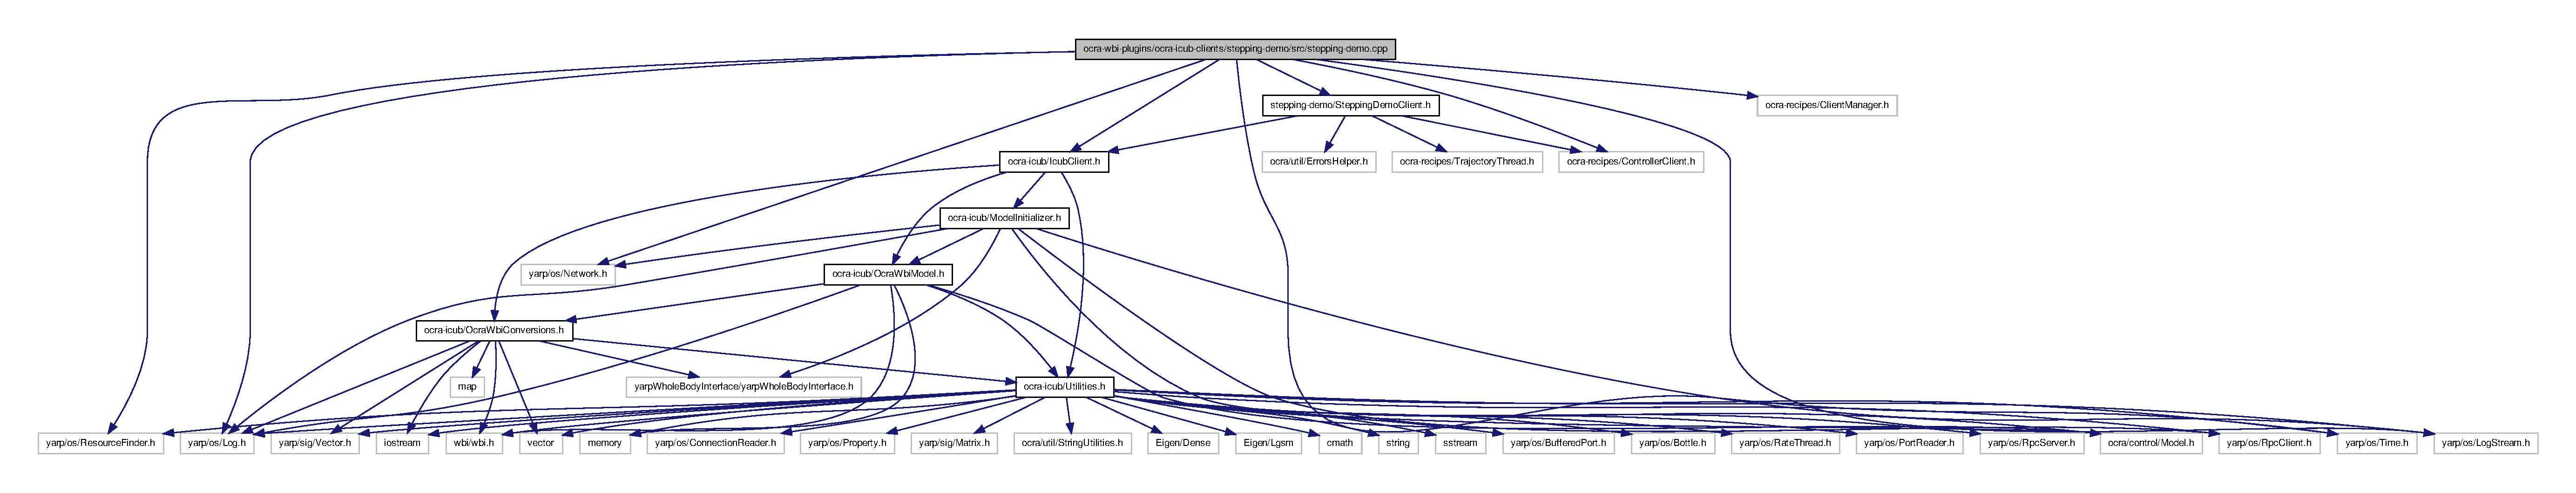
\includegraphics[width=350pt]{stepping-demo_8cpp__incl}
\end{center}
\end{figure}
\subsection*{\-Functions}
\begin{DoxyCompactItemize}
\item 
int \hyperlink{stepping-demo_8cpp_a0ddf1224851353fc92bfbff6f499fa97}{main} (int argc, char $\ast$argv\mbox{[}$\,$\mbox{]})
\end{DoxyCompactItemize}


\subsection{\-Detailed \-Description}
\begin{DoxyAuthor}{\-Author}
\mbox{[}\-Ryan \-Lober\mbox{]}(\href{http://www.ryanlober.com}{\tt http\-://www.\-ryanlober.\-com}) 

\mbox{[}\-Antoine \-Hoarau\mbox{]}(\href{http://ahoarau.github.io}{\tt http\-://ahoarau.\-github.\-io}) 

\mbox{[}\-Jorhabib \-Eljaik\mbox{]}(\href{https://github.com/jeljaik}{\tt https\-://github.\-com/jeljaik}) 
\end{DoxyAuthor}
\begin{DoxyDate}{\-Date}
\-Feb 2016 
\end{DoxyDate}
\begin{DoxyCopyright}{\-Copyright}
\-G\-N\-U \-General \-Public \-License. 
\end{DoxyCopyright}


\subsection{\-Function \-Documentation}
\hypertarget{stepping-demo_8cpp_a0ddf1224851353fc92bfbff6f499fa97}{\index{stepping-\/demo.\-cpp@{stepping-\/demo.\-cpp}!main@{main}}
\index{main@{main}!stepping-demo.cpp@{stepping-\/demo.\-cpp}}
\subsubsection[{main}]{\setlength{\rightskip}{0pt plus 5cm}int {\bf main} (
\begin{DoxyParamCaption}
\item[{int}]{argc, }
\item[{char $\ast$}]{argv\mbox{[}$\,$\mbox{]}}
\end{DoxyParamCaption}
)}}\label{stepping-demo_8cpp_a0ddf1224851353fc92bfbff6f499fa97}

\hypertarget{SteppingDemoClient_8cpp}{\section{ocra-\/wbi-\/plugins/ocra-\/icub-\/clients/stepping-\/demo/src/\-Stepping\-Demo\-Client.cpp \-File \-Reference}
\label{SteppingDemoClient_8cpp}\index{ocra-\/wbi-\/plugins/ocra-\/icub-\/clients/stepping-\/demo/src/\-Stepping\-Demo\-Client.\-cpp@{ocra-\/wbi-\/plugins/ocra-\/icub-\/clients/stepping-\/demo/src/\-Stepping\-Demo\-Client.\-cpp}}
}
{\ttfamily \#include \char`\"{}stepping-\/demo/\-Stepping\-Demo\-Client.\-h\char`\"{}}\*
\-Include dependency graph for \-Stepping\-Demo\-Client.\-cpp\-:\nopagebreak
\begin{figure}[H]
\begin{center}
\leavevmode
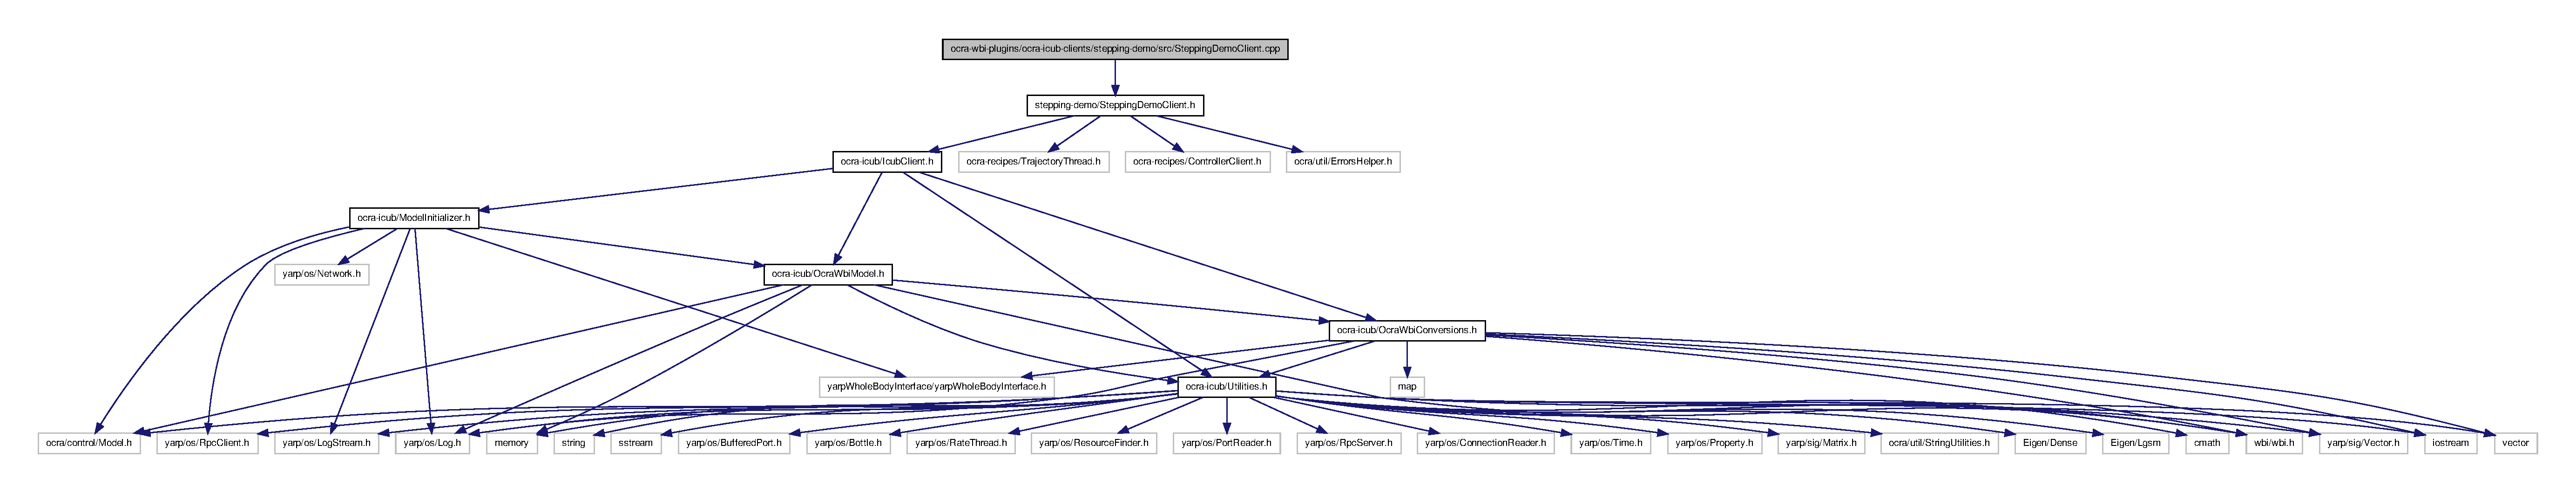
\includegraphics[width=350pt]{SteppingDemoClient_8cpp__incl}
\end{center}
\end{figure}

\hypertarget{TaskOpsClient_8h}{\section{ocra-\/wbi-\/plugins/ocra-\/icub-\/clients/task-\/operations-\/demo/include/task-\/operations-\/demo/\-Task\-Ops\-Client.h \-File \-Reference}
\label{TaskOpsClient_8h}\index{ocra-\/wbi-\/plugins/ocra-\/icub-\/clients/task-\/operations-\/demo/include/task-\/operations-\/demo/\-Task\-Ops\-Client.\-h@{ocra-\/wbi-\/plugins/ocra-\/icub-\/clients/task-\/operations-\/demo/include/task-\/operations-\/demo/\-Task\-Ops\-Client.\-h}}
}
{\ttfamily \#include $<$ocra-\/icub/\-Icub\-Client.\-h$>$}\*
{\ttfamily \#include $<$ocra-\/recipes/\-Trajectory\-Thread.\-h$>$}\*
{\ttfamily \#include $<$ocra-\/recipes/\-Controller\-Client.\-h$>$}\*
\-Include dependency graph for \-Task\-Ops\-Client.\-h\-:\nopagebreak
\begin{figure}[H]
\begin{center}
\leavevmode
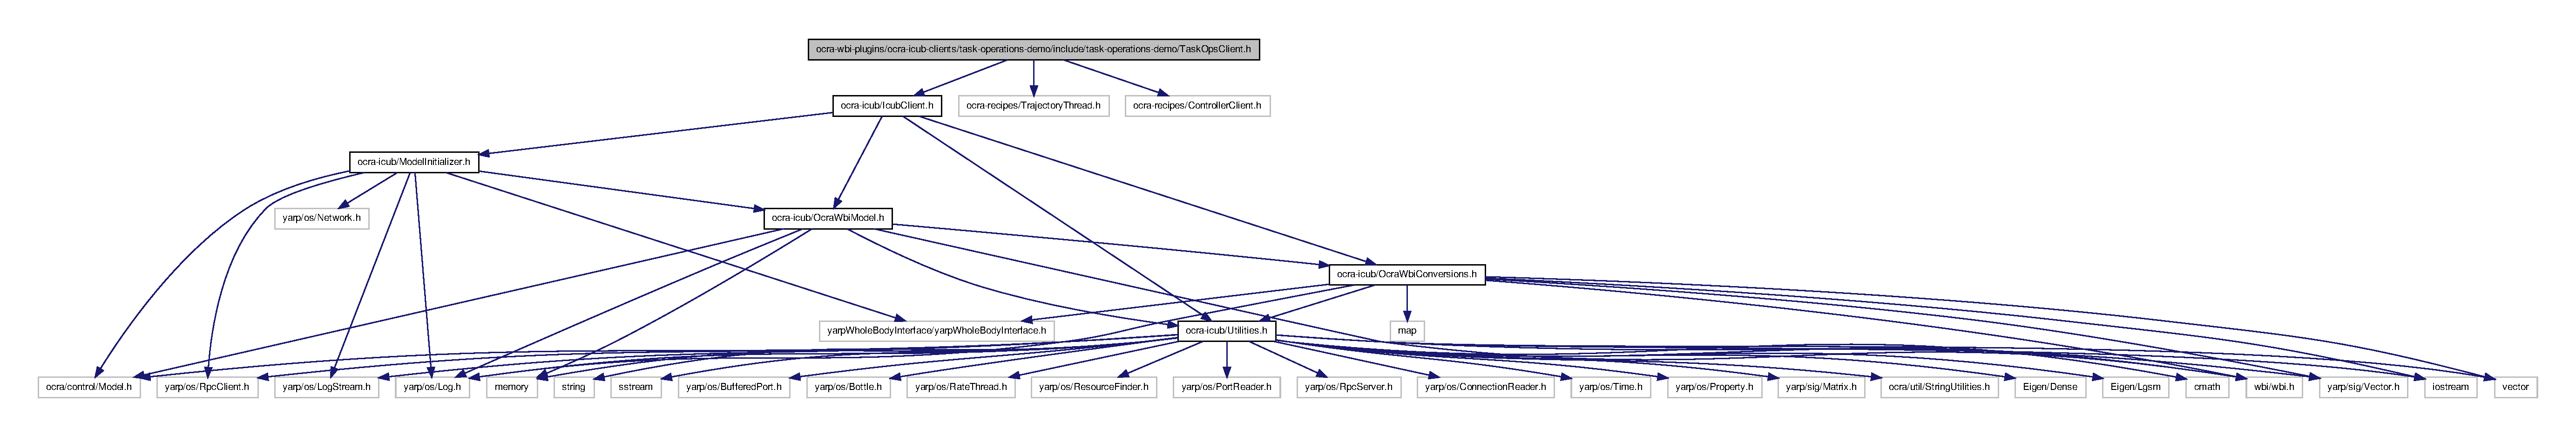
\includegraphics[width=350pt]{TaskOpsClient_8h__incl}
\end{center}
\end{figure}
\-This graph shows which files directly or indirectly include this file\-:\nopagebreak
\begin{figure}[H]
\begin{center}
\leavevmode
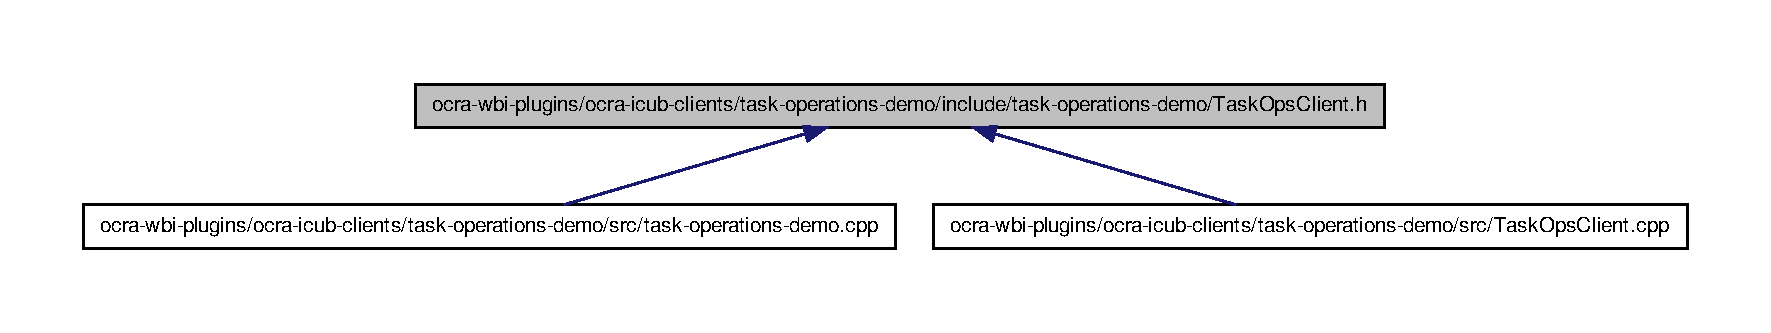
\includegraphics[width=350pt]{TaskOpsClient_8h__dep__incl}
\end{center}
\end{figure}
\subsection*{\-Classes}
\begin{DoxyCompactItemize}
\item 
class \hyperlink{classTaskOpsClient}{\-Task\-Ops\-Client}
\end{DoxyCompactItemize}
\subsection*{\-Enumerations}
\begin{DoxyCompactItemize}
\item 
enum \hyperlink{TaskOpsClient_8h_a0140057ae3fbe1db5f5c418dfc67d9db}{\-T\-H\-I\-N\-G\-S\-\_\-\-T\-O\-\_\-\-D\-O} \{ \*
\hyperlink{TaskOpsClient_8h_a0140057ae3fbe1db5f5c418dfc67d9dbaf831abed77e2c76cacc256b8b16f2b2a}{\-R\-E\-M\-O\-V\-E\-\_\-\-T\-A\-S\-K}, 
\hyperlink{TaskOpsClient_8h_a0140057ae3fbe1db5f5c418dfc67d9dba6aa666a68fed72da5438e0ef9b7cba8f}{\-A\-D\-D\-\_\-\-N\-E\-W\-\_\-\-T\-A\-S\-K}, 
\hyperlink{TaskOpsClient_8h_a0140057ae3fbe1db5f5c418dfc67d9dba8ffc9eba853106ab798ee2a0c5763d1b}{\-A\-D\-D\-\_\-\-E\-X\-I\-S\-T\-I\-N\-G\-\_\-\-T\-A\-S\-K}, 
\hyperlink{TaskOpsClient_8h_a0140057ae3fbe1db5f5c418dfc67d9dba7eaf30861bc723f003ea1a8e4a7a4977}{\-A\-D\-D\-\_\-\-E\-X\-I\-S\-T\-I\-N\-G\-\_\-\-T\-A\-S\-K\-\_\-\-N\-O\-\_\-\-O\-V\-E\-R\-W\-R\-I\-T\-E}, 
\*
\hyperlink{TaskOpsClient_8h_a0140057ae3fbe1db5f5c418dfc67d9dbacfe24a7b308a82835c8a9a9a89bc4ca2}{\-N\-O\-T\-H\-I\-N\-G}
 \}
\end{DoxyCompactItemize}


\subsection{\-Enumeration \-Type \-Documentation}
\hypertarget{TaskOpsClient_8h_a0140057ae3fbe1db5f5c418dfc67d9db}{\index{\-Task\-Ops\-Client.\-h@{\-Task\-Ops\-Client.\-h}!\-T\-H\-I\-N\-G\-S\-\_\-\-T\-O\-\_\-\-D\-O@{\-T\-H\-I\-N\-G\-S\-\_\-\-T\-O\-\_\-\-D\-O}}
\index{\-T\-H\-I\-N\-G\-S\-\_\-\-T\-O\-\_\-\-D\-O@{\-T\-H\-I\-N\-G\-S\-\_\-\-T\-O\-\_\-\-D\-O}!TaskOpsClient.h@{\-Task\-Ops\-Client.\-h}}
\subsubsection[{\-T\-H\-I\-N\-G\-S\-\_\-\-T\-O\-\_\-\-D\-O}]{\setlength{\rightskip}{0pt plus 5cm}enum {\bf \-T\-H\-I\-N\-G\-S\-\_\-\-T\-O\-\_\-\-D\-O}}}\label{TaskOpsClient_8h_a0140057ae3fbe1db5f5c418dfc67d9db}
\begin{Desc}
\item[\-Enumerator\-: ]\par
\begin{description}
\index{\-R\-E\-M\-O\-V\-E\-\_\-\-T\-A\-S\-K@{\-R\-E\-M\-O\-V\-E\-\_\-\-T\-A\-S\-K}!\-Task\-Ops\-Client.\-h@{\-Task\-Ops\-Client.\-h}}\index{\-Task\-Ops\-Client.\-h@{\-Task\-Ops\-Client.\-h}!\-R\-E\-M\-O\-V\-E\-\_\-\-T\-A\-S\-K@{\-R\-E\-M\-O\-V\-E\-\_\-\-T\-A\-S\-K}}\item[{\em 
\hypertarget{TaskOpsClient_8h_a0140057ae3fbe1db5f5c418dfc67d9dbaf831abed77e2c76cacc256b8b16f2b2a}{\-R\-E\-M\-O\-V\-E\-\_\-\-T\-A\-S\-K}\label{TaskOpsClient_8h_a0140057ae3fbe1db5f5c418dfc67d9dbaf831abed77e2c76cacc256b8b16f2b2a}
}]\index{\-A\-D\-D\-\_\-\-N\-E\-W\-\_\-\-T\-A\-S\-K@{\-A\-D\-D\-\_\-\-N\-E\-W\-\_\-\-T\-A\-S\-K}!\-Task\-Ops\-Client.\-h@{\-Task\-Ops\-Client.\-h}}\index{\-Task\-Ops\-Client.\-h@{\-Task\-Ops\-Client.\-h}!\-A\-D\-D\-\_\-\-N\-E\-W\-\_\-\-T\-A\-S\-K@{\-A\-D\-D\-\_\-\-N\-E\-W\-\_\-\-T\-A\-S\-K}}\item[{\em 
\hypertarget{TaskOpsClient_8h_a0140057ae3fbe1db5f5c418dfc67d9dba6aa666a68fed72da5438e0ef9b7cba8f}{\-A\-D\-D\-\_\-\-N\-E\-W\-\_\-\-T\-A\-S\-K}\label{TaskOpsClient_8h_a0140057ae3fbe1db5f5c418dfc67d9dba6aa666a68fed72da5438e0ef9b7cba8f}
}]\index{\-A\-D\-D\-\_\-\-E\-X\-I\-S\-T\-I\-N\-G\-\_\-\-T\-A\-S\-K@{\-A\-D\-D\-\_\-\-E\-X\-I\-S\-T\-I\-N\-G\-\_\-\-T\-A\-S\-K}!\-Task\-Ops\-Client.\-h@{\-Task\-Ops\-Client.\-h}}\index{\-Task\-Ops\-Client.\-h@{\-Task\-Ops\-Client.\-h}!\-A\-D\-D\-\_\-\-E\-X\-I\-S\-T\-I\-N\-G\-\_\-\-T\-A\-S\-K@{\-A\-D\-D\-\_\-\-E\-X\-I\-S\-T\-I\-N\-G\-\_\-\-T\-A\-S\-K}}\item[{\em 
\hypertarget{TaskOpsClient_8h_a0140057ae3fbe1db5f5c418dfc67d9dba8ffc9eba853106ab798ee2a0c5763d1b}{\-A\-D\-D\-\_\-\-E\-X\-I\-S\-T\-I\-N\-G\-\_\-\-T\-A\-S\-K}\label{TaskOpsClient_8h_a0140057ae3fbe1db5f5c418dfc67d9dba8ffc9eba853106ab798ee2a0c5763d1b}
}]\index{\-A\-D\-D\-\_\-\-E\-X\-I\-S\-T\-I\-N\-G\-\_\-\-T\-A\-S\-K\-\_\-\-N\-O\-\_\-\-O\-V\-E\-R\-W\-R\-I\-T\-E@{\-A\-D\-D\-\_\-\-E\-X\-I\-S\-T\-I\-N\-G\-\_\-\-T\-A\-S\-K\-\_\-\-N\-O\-\_\-\-O\-V\-E\-R\-W\-R\-I\-T\-E}!\-Task\-Ops\-Client.\-h@{\-Task\-Ops\-Client.\-h}}\index{\-Task\-Ops\-Client.\-h@{\-Task\-Ops\-Client.\-h}!\-A\-D\-D\-\_\-\-E\-X\-I\-S\-T\-I\-N\-G\-\_\-\-T\-A\-S\-K\-\_\-\-N\-O\-\_\-\-O\-V\-E\-R\-W\-R\-I\-T\-E@{\-A\-D\-D\-\_\-\-E\-X\-I\-S\-T\-I\-N\-G\-\_\-\-T\-A\-S\-K\-\_\-\-N\-O\-\_\-\-O\-V\-E\-R\-W\-R\-I\-T\-E}}\item[{\em 
\hypertarget{TaskOpsClient_8h_a0140057ae3fbe1db5f5c418dfc67d9dba7eaf30861bc723f003ea1a8e4a7a4977}{\-A\-D\-D\-\_\-\-E\-X\-I\-S\-T\-I\-N\-G\-\_\-\-T\-A\-S\-K\-\_\-\-N\-O\-\_\-\-O\-V\-E\-R\-W\-R\-I\-T\-E}\label{TaskOpsClient_8h_a0140057ae3fbe1db5f5c418dfc67d9dba7eaf30861bc723f003ea1a8e4a7a4977}
}]\index{\-N\-O\-T\-H\-I\-N\-G@{\-N\-O\-T\-H\-I\-N\-G}!\-Task\-Ops\-Client.\-h@{\-Task\-Ops\-Client.\-h}}\index{\-Task\-Ops\-Client.\-h@{\-Task\-Ops\-Client.\-h}!\-N\-O\-T\-H\-I\-N\-G@{\-N\-O\-T\-H\-I\-N\-G}}\item[{\em 
\hypertarget{TaskOpsClient_8h_a0140057ae3fbe1db5f5c418dfc67d9dbacfe24a7b308a82835c8a9a9a89bc4ca2}{\-N\-O\-T\-H\-I\-N\-G}\label{TaskOpsClient_8h_a0140057ae3fbe1db5f5c418dfc67d9dbacfe24a7b308a82835c8a9a9a89bc4ca2}
}]\end{description}
\end{Desc}


\hypertarget{task-operations-demo_8cpp}{\section{ocra-\/wbi-\/plugins/ocra-\/icub-\/clients/task-\/operations-\/demo/src/task-\/operations-\/demo.cpp \-File \-Reference}
\label{task-operations-demo_8cpp}\index{ocra-\/wbi-\/plugins/ocra-\/icub-\/clients/task-\/operations-\/demo/src/task-\/operations-\/demo.\-cpp@{ocra-\/wbi-\/plugins/ocra-\/icub-\/clients/task-\/operations-\/demo/src/task-\/operations-\/demo.\-cpp}}
}
{\ttfamily \#include $<$yarp/os/\-Resource\-Finder.\-h$>$}\*
{\ttfamily \#include $<$yarp/os/\-Network.\-h$>$}\*
{\ttfamily \#include $<$yarp/os/\-Log.\-h$>$}\*
{\ttfamily \#include $<$yarp/os/\-Log\-Stream.\-h$>$}\*
{\ttfamily \#include $<$yarp/os/\-Time.\-h$>$}\*
{\ttfamily \#include \char`\"{}task-\/operations-\/demo/\-Task\-Ops\-Client.\-h\char`\"{}}\*
{\ttfamily \#include $<$ocra-\/icub/\-Icub\-Client.\-h$>$}\*
{\ttfamily \#include $<$ocra-\/recipes/\-Controller\-Client.\-h$>$}\*
{\ttfamily \#include $<$ocra-\/recipes/\-Client\-Manager.\-h$>$}\*
\-Include dependency graph for task-\/operations-\/demo.cpp\-:
\nopagebreak
\begin{figure}[H]
\begin{center}
\leavevmode
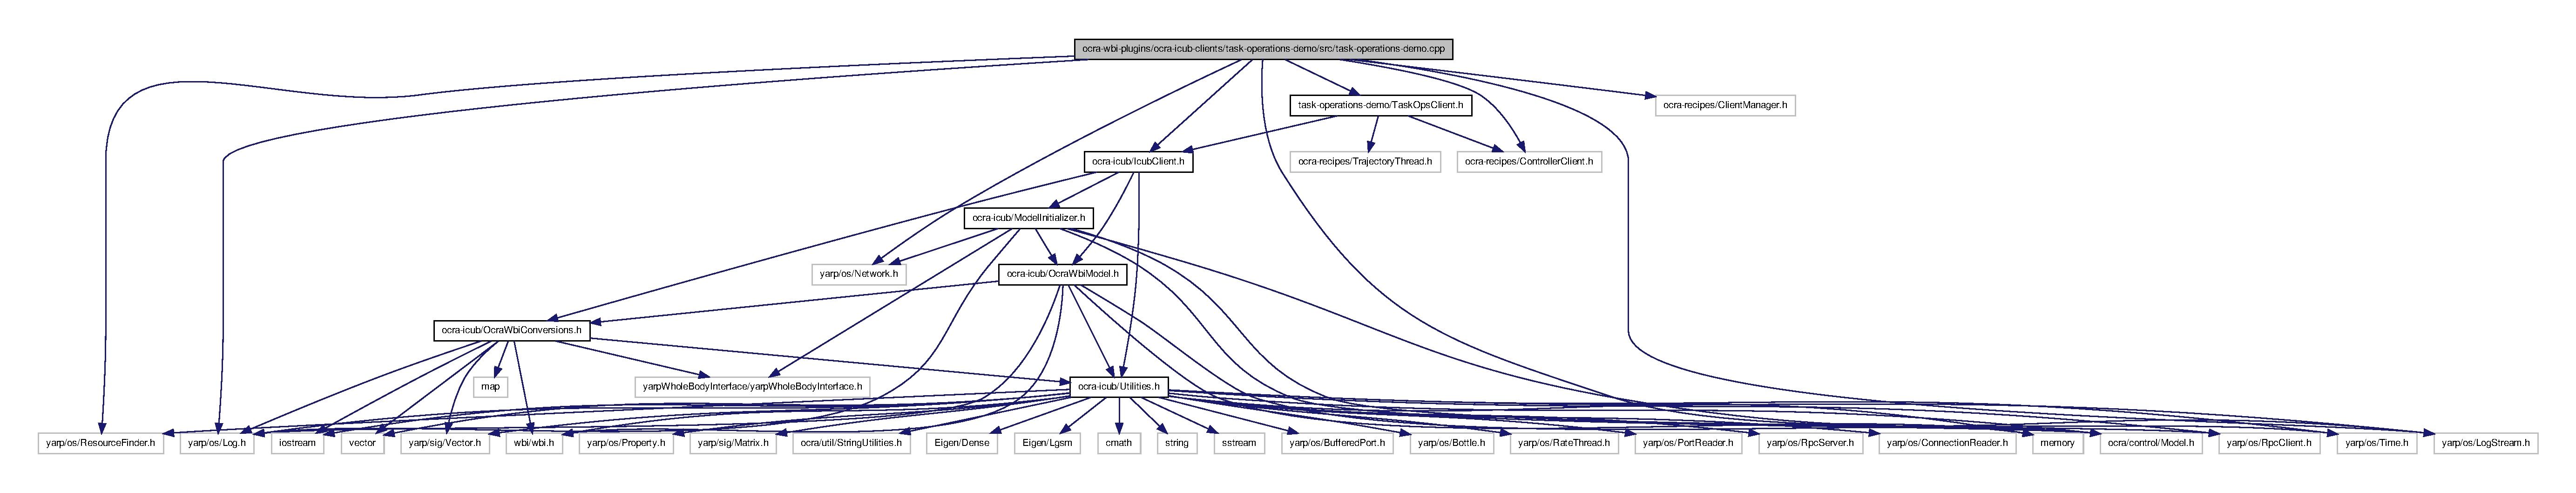
\includegraphics[width=350pt]{task-operations-demo_8cpp__incl}
\end{center}
\end{figure}
\subsection*{\-Functions}
\begin{DoxyCompactItemize}
\item 
int \hyperlink{task-operations-demo_8cpp_a0ddf1224851353fc92bfbff6f499fa97}{main} (int argc, char $\ast$argv\mbox{[}$\,$\mbox{]})
\end{DoxyCompactItemize}


\subsection{\-Function \-Documentation}
\hypertarget{task-operations-demo_8cpp_a0ddf1224851353fc92bfbff6f499fa97}{\index{task-\/operations-\/demo.\-cpp@{task-\/operations-\/demo.\-cpp}!main@{main}}
\index{main@{main}!task-operations-demo.cpp@{task-\/operations-\/demo.\-cpp}}
\subsubsection[{main}]{\setlength{\rightskip}{0pt plus 5cm}int {\bf main} (
\begin{DoxyParamCaption}
\item[{int}]{argc, }
\item[{char $\ast$}]{argv\mbox{[}$\,$\mbox{]}}
\end{DoxyParamCaption}
)}}\label{task-operations-demo_8cpp_a0ddf1224851353fc92bfbff6f499fa97}

\hypertarget{TaskOpsClient_8cpp}{\section{ocra-\/wbi-\/plugins/ocra-\/icub-\/clients/task-\/operations-\/demo/src/\-Task\-Ops\-Client.cpp \-File \-Reference}
\label{TaskOpsClient_8cpp}\index{ocra-\/wbi-\/plugins/ocra-\/icub-\/clients/task-\/operations-\/demo/src/\-Task\-Ops\-Client.\-cpp@{ocra-\/wbi-\/plugins/ocra-\/icub-\/clients/task-\/operations-\/demo/src/\-Task\-Ops\-Client.\-cpp}}
}
{\ttfamily \#include \char`\"{}task-\/operations-\/demo/\-Task\-Ops\-Client.\-h\char`\"{}}\*
\-Include dependency graph for \-Task\-Ops\-Client.\-cpp\-:
\nopagebreak
\begin{figure}[H]
\begin{center}
\leavevmode
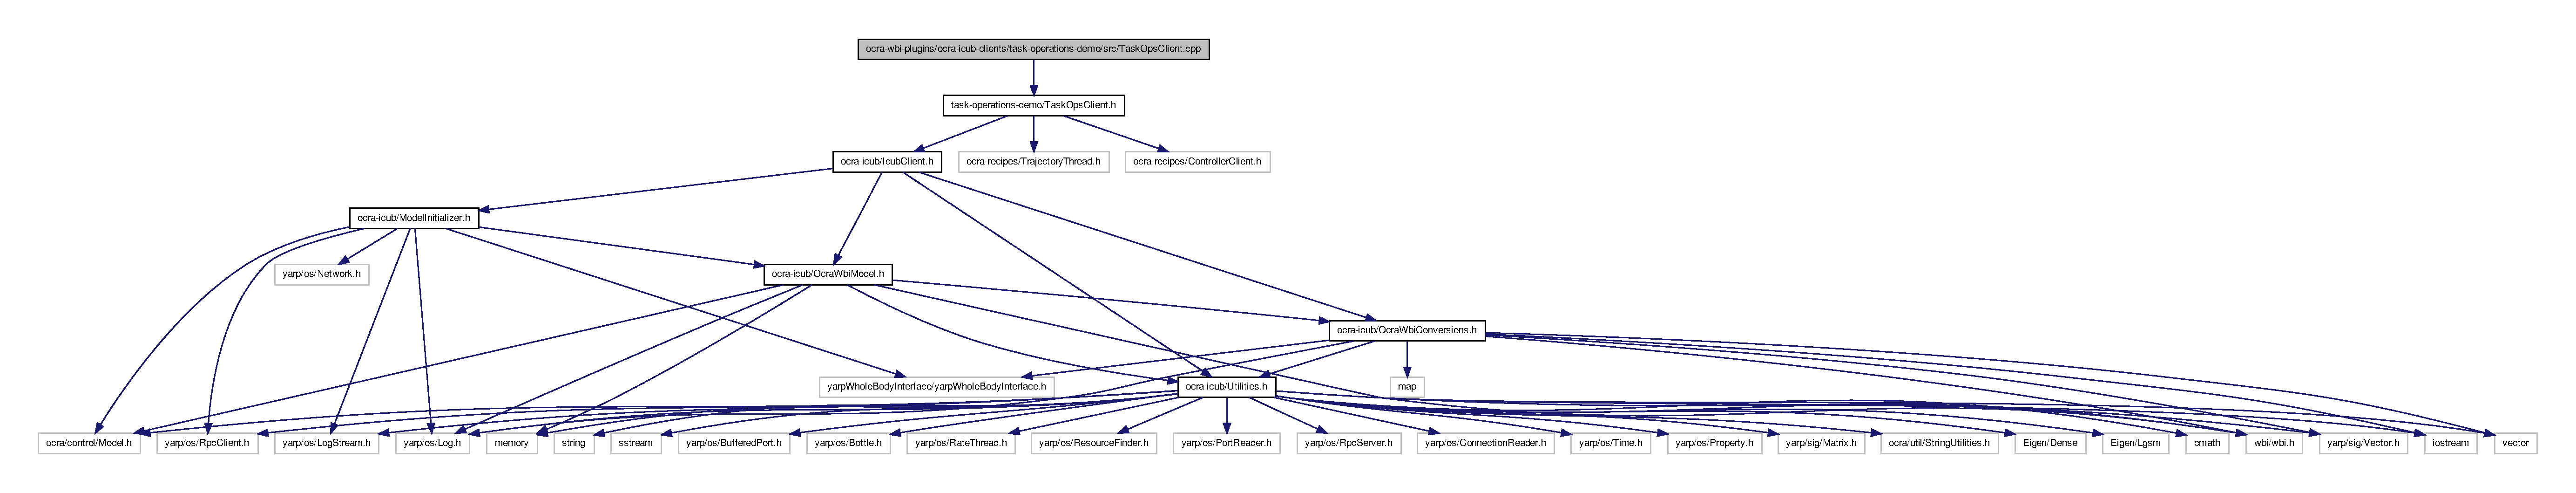
\includegraphics[width=350pt]{TaskOpsClient_8cpp__incl}
\end{center}
\end{figure}

\hypertarget{WalkingClient_8h}{\section{ocra-\/wbi-\/plugins/ocra-\/icub-\/clients/walking-\/client/include/walking-\/client/\-Walking\-Client.h \-File \-Reference}
\label{WalkingClient_8h}\index{ocra-\/wbi-\/plugins/ocra-\/icub-\/clients/walking-\/client/include/walking-\/client/\-Walking\-Client.\-h@{ocra-\/wbi-\/plugins/ocra-\/icub-\/clients/walking-\/client/include/walking-\/client/\-Walking\-Client.\-h}}
}
{\ttfamily \#include $<$ocra-\/icub/\-Icub\-Client.\-h$>$}\*
{\ttfamily \#include $<$ocra-\/recipes/\-Trajectory\-Thread.\-h$>$}\*
{\ttfamily \#include $<$ocra-\/recipes/\-Controller\-Client.\-h$>$}\*
{\ttfamily \#include $<$ocra/util/\-Eigen\-Utilities.\-h$>$}\*
{\ttfamily \#include \char`\"{}walking-\/client/\-Zmp\-Preview\-Controller.\-h\char`\"{}}\*
{\ttfamily \#include \char`\"{}walking-\/client/\-Zmp\-Controller.\-h\char`\"{}}\*
{\ttfamily \#include $<$ocra/util/\-File\-Operations.\-h$>$}\*
{\ttfamily \#include $<$yarp/os/\-Time.\-h$>$}\*
\-Include dependency graph for \-Walking\-Client.\-h\-:
\nopagebreak
\begin{figure}[H]
\begin{center}
\leavevmode
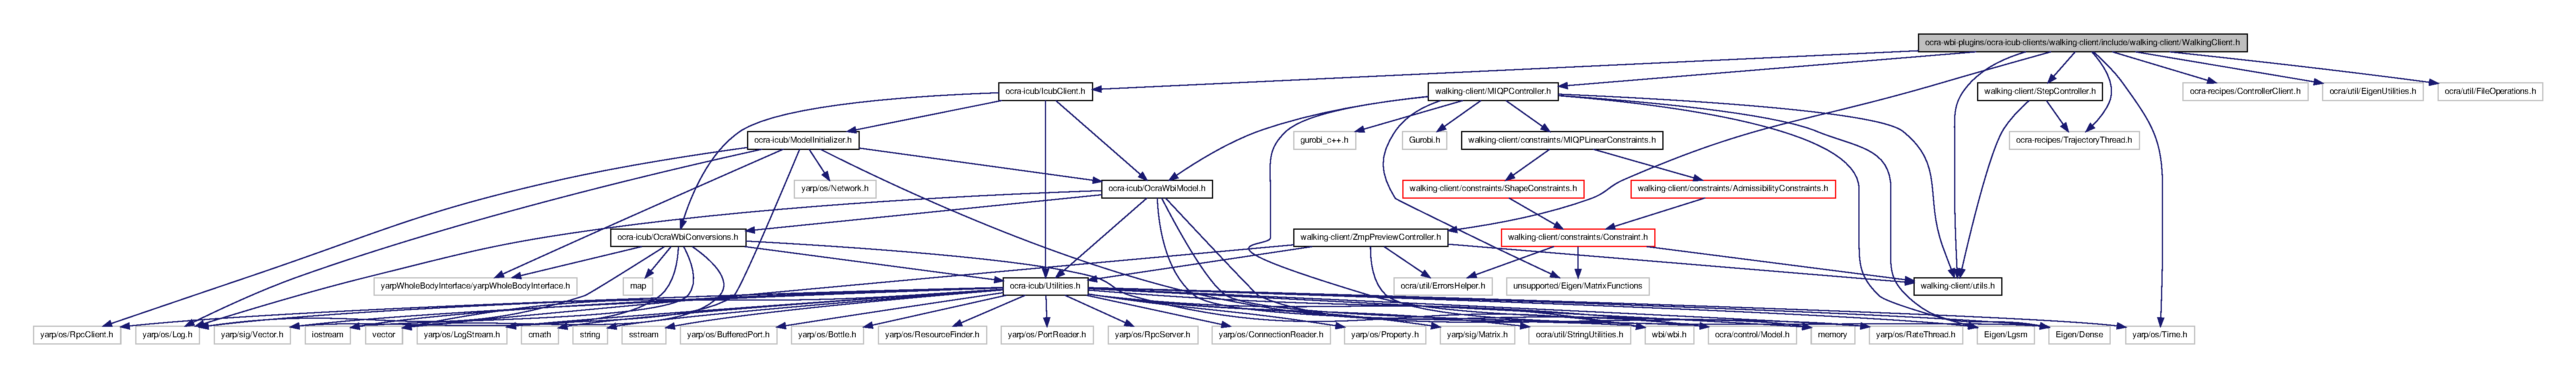
\includegraphics[width=350pt]{WalkingClient_8h__incl}
\end{center}
\end{figure}
\-This graph shows which files directly or indirectly include this file\-:
\nopagebreak
\begin{figure}[H]
\begin{center}
\leavevmode
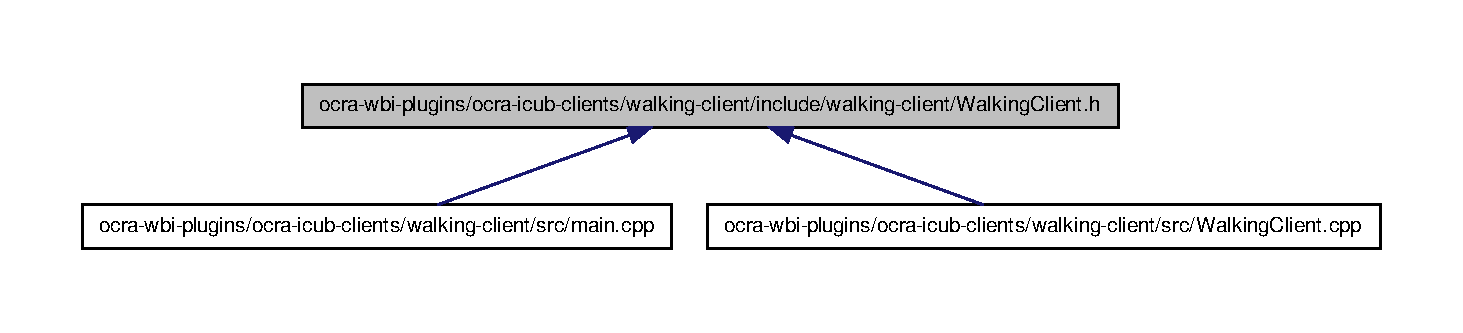
\includegraphics[width=350pt]{WalkingClient_8h__dep__incl}
\end{center}
\end{figure}
\subsection*{\-Classes}
\begin{DoxyCompactItemize}
\item 
class \hyperlink{classWalkingClient}{\-Walking\-Client}
\end{DoxyCompactItemize}
\subsection*{\-Enumerations}
\begin{DoxyCompactItemize}
\item 
enum \hyperlink{WalkingClient_8h_afc01479a47f5a87462a54b6a9e11fffa}{\-Zmp\-Test\-Type} \{ \hyperlink{WalkingClient_8h_afc01479a47f5a87462a54b6a9e11fffaa648ff770c850b8352c3306c1659e8157}{\-Z\-M\-P\-\_\-\-C\-O\-N\-S\-T\-A\-N\-T\-\_\-\-R\-E\-F\-E\-R\-E\-N\-C\-E} = 0, 
\hyperlink{WalkingClient_8h_afc01479a47f5a87462a54b6a9e11fffaa97cb99b5fec95c1f2945d3b33455b139}{\-Z\-M\-P\-\_\-\-V\-A\-R\-Y\-I\-N\-G\-\_\-\-R\-E\-F\-E\-R\-E\-N\-C\-E}, 
\hyperlink{WalkingClient_8h_afc01479a47f5a87462a54b6a9e11fffaad20e2ca429f4e3ba50e1de174c92af60}{\-C\-O\-M\-\_\-\-L\-I\-N\-\_\-\-V\-E\-L\-\_\-\-C\-O\-N\-S\-T\-A\-N\-T\-\_\-\-R\-E\-F\-E\-R\-E\-N\-C\-E}
 \}
\end{DoxyCompactItemize}


\subsection{\-Enumeration \-Type \-Documentation}
\hypertarget{WalkingClient_8h_afc01479a47f5a87462a54b6a9e11fffa}{\index{\-Walking\-Client.\-h@{\-Walking\-Client.\-h}!\-Zmp\-Test\-Type@{\-Zmp\-Test\-Type}}
\index{\-Zmp\-Test\-Type@{\-Zmp\-Test\-Type}!WalkingClient.h@{\-Walking\-Client.\-h}}
\subsubsection[{\-Zmp\-Test\-Type}]{\setlength{\rightskip}{0pt plus 5cm}enum {\bf \-Zmp\-Test\-Type}}}\label{WalkingClient_8h_afc01479a47f5a87462a54b6a9e11fffa}
\-Performs tests helpful to tune the gains used by the zmp and zmp preview controllers as well as the \-C\-O\-M task. \-See configure() for additional information. \begin{Desc}
\item[\-Enumerator\-: ]\par
\begin{description}
\index{\-Z\-M\-P\-\_\-\-C\-O\-N\-S\-T\-A\-N\-T\-\_\-\-R\-E\-F\-E\-R\-E\-N\-C\-E@{\-Z\-M\-P\-\_\-\-C\-O\-N\-S\-T\-A\-N\-T\-\_\-\-R\-E\-F\-E\-R\-E\-N\-C\-E}!\-Walking\-Client.\-h@{\-Walking\-Client.\-h}}\index{\-Walking\-Client.\-h@{\-Walking\-Client.\-h}!\-Z\-M\-P\-\_\-\-C\-O\-N\-S\-T\-A\-N\-T\-\_\-\-R\-E\-F\-E\-R\-E\-N\-C\-E@{\-Z\-M\-P\-\_\-\-C\-O\-N\-S\-T\-A\-N\-T\-\_\-\-R\-E\-F\-E\-R\-E\-N\-C\-E}}\item[{\em 
\hypertarget{WalkingClient_8h_afc01479a47f5a87462a54b6a9e11fffaa648ff770c850b8352c3306c1659e8157}{\-Z\-M\-P\-\_\-\-C\-O\-N\-S\-T\-A\-N\-T\-\_\-\-R\-E\-F\-E\-R\-E\-N\-C\-E}\label{WalkingClient_8h_afc01479a47f5a87462a54b6a9e11fffaa648ff770c850b8352c3306c1659e8157}
}]\index{\-Z\-M\-P\-\_\-\-V\-A\-R\-Y\-I\-N\-G\-\_\-\-R\-E\-F\-E\-R\-E\-N\-C\-E@{\-Z\-M\-P\-\_\-\-V\-A\-R\-Y\-I\-N\-G\-\_\-\-R\-E\-F\-E\-R\-E\-N\-C\-E}!\-Walking\-Client.\-h@{\-Walking\-Client.\-h}}\index{\-Walking\-Client.\-h@{\-Walking\-Client.\-h}!\-Z\-M\-P\-\_\-\-V\-A\-R\-Y\-I\-N\-G\-\_\-\-R\-E\-F\-E\-R\-E\-N\-C\-E@{\-Z\-M\-P\-\_\-\-V\-A\-R\-Y\-I\-N\-G\-\_\-\-R\-E\-F\-E\-R\-E\-N\-C\-E}}\item[{\em 
\hypertarget{WalkingClient_8h_afc01479a47f5a87462a54b6a9e11fffaa97cb99b5fec95c1f2945d3b33455b139}{\-Z\-M\-P\-\_\-\-V\-A\-R\-Y\-I\-N\-G\-\_\-\-R\-E\-F\-E\-R\-E\-N\-C\-E}\label{WalkingClient_8h_afc01479a47f5a87462a54b6a9e11fffaa97cb99b5fec95c1f2945d3b33455b139}
}]\index{\-C\-O\-M\-\_\-\-L\-I\-N\-\_\-\-V\-E\-L\-\_\-\-C\-O\-N\-S\-T\-A\-N\-T\-\_\-\-R\-E\-F\-E\-R\-E\-N\-C\-E@{\-C\-O\-M\-\_\-\-L\-I\-N\-\_\-\-V\-E\-L\-\_\-\-C\-O\-N\-S\-T\-A\-N\-T\-\_\-\-R\-E\-F\-E\-R\-E\-N\-C\-E}!\-Walking\-Client.\-h@{\-Walking\-Client.\-h}}\index{\-Walking\-Client.\-h@{\-Walking\-Client.\-h}!\-C\-O\-M\-\_\-\-L\-I\-N\-\_\-\-V\-E\-L\-\_\-\-C\-O\-N\-S\-T\-A\-N\-T\-\_\-\-R\-E\-F\-E\-R\-E\-N\-C\-E@{\-C\-O\-M\-\_\-\-L\-I\-N\-\_\-\-V\-E\-L\-\_\-\-C\-O\-N\-S\-T\-A\-N\-T\-\_\-\-R\-E\-F\-E\-R\-E\-N\-C\-E}}\item[{\em 
\hypertarget{WalkingClient_8h_afc01479a47f5a87462a54b6a9e11fffaad20e2ca429f4e3ba50e1de174c92af60}{\-C\-O\-M\-\_\-\-L\-I\-N\-\_\-\-V\-E\-L\-\_\-\-C\-O\-N\-S\-T\-A\-N\-T\-\_\-\-R\-E\-F\-E\-R\-E\-N\-C\-E}\label{WalkingClient_8h_afc01479a47f5a87462a54b6a9e11fffaad20e2ca429f4e3ba50e1de174c92af60}
}]\end{description}
\end{Desc}


\hypertarget{ZmpController_8h}{\section{ocra-\/wbi-\/plugins/ocra-\/icub-\/clients/walking-\/client/include/walking-\/client/\-Zmp\-Controller.h \-File \-Reference}
\label{ZmpController_8h}\index{ocra-\/wbi-\/plugins/ocra-\/icub-\/clients/walking-\/client/include/walking-\/client/\-Zmp\-Controller.\-h@{ocra-\/wbi-\/plugins/ocra-\/icub-\/clients/walking-\/client/include/walking-\/client/\-Zmp\-Controller.\-h}}
}
{\ttfamily \#include $<$ocra-\/icub/\-Utilities.\-h$>$}\*
{\ttfamily \#include $<$ocra/util/\-Errors\-Helper.\-h$>$}\*
{\ttfamily \#include $<$ocra/util/\-Eigen\-Utilities.\-h$>$}\*
{\ttfamily \#include $<$ocra/control/\-Task\-State.\-h$>$}\*
{\ttfamily \#include $<$ocra-\/recipes/\-Task\-Connection.\-h$>$}\*
{\ttfamily \#include $<$\-Eigen/\-Dense$>$}\*
{\ttfamily \#include $<$vector$>$}\*
\-Include dependency graph for \-Zmp\-Controller.\-h\-:\nopagebreak
\begin{figure}[H]
\begin{center}
\leavevmode
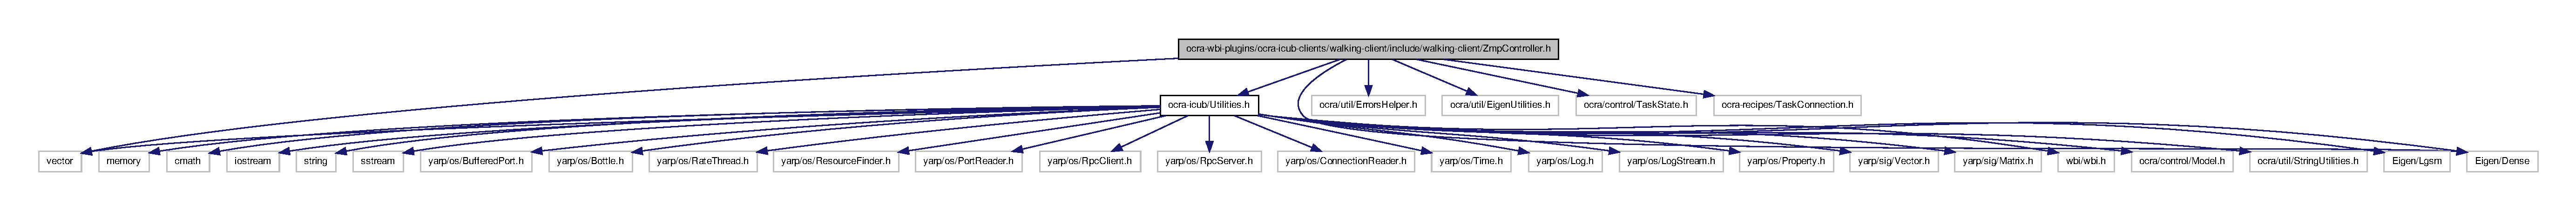
\includegraphics[width=350pt]{ZmpController_8h__incl}
\end{center}
\end{figure}
\-This graph shows which files directly or indirectly include this file\-:\nopagebreak
\begin{figure}[H]
\begin{center}
\leavevmode
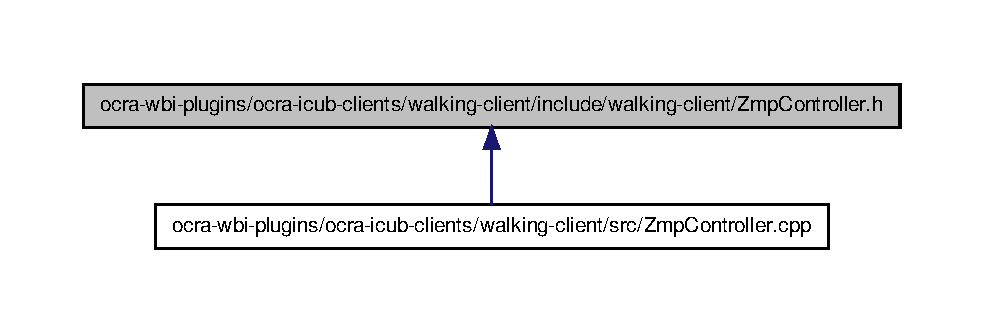
\includegraphics[width=350pt]{ZmpController_8h__dep__incl}
\end{center}
\end{figure}
\subsection*{\-Classes}
\begin{DoxyCompactItemize}
\item 
struct \hyperlink{structZmpControllerParams}{\-Zmp\-Controller\-Params}
\item 
class \hyperlink{classZmpController}{\-Zmp\-Controller}
\begin{DoxyCompactList}\small\item\em \-Implementes a \-Z\-M\-P controller as a force set point regulator. \end{DoxyCompactList}\end{DoxyCompactItemize}
\subsection*{\-Enumerations}
\begin{DoxyCompactItemize}
\item 
enum \hyperlink{ZmpController_8h_a4b6a8e135f90bd56e5a57a60efb42529}{\-F\-O\-O\-T} \{ \hyperlink{ZmpController_8h_a4b6a8e135f90bd56e5a57a60efb42529a7760daad9db1ede8c57b06189deca9f3}{\-L\-E\-F\-T\-\_\-\-F\-O\-O\-T}, 
\hyperlink{ZmpController_8h_a4b6a8e135f90bd56e5a57a60efb42529ace119c66af60ac0781b137aa87d7be62}{\-R\-I\-G\-H\-T\-\_\-\-F\-O\-O\-T}
 \}
\end{DoxyCompactItemize}


\subsection{\-Enumeration \-Type \-Documentation}
\hypertarget{ZmpController_8h_a4b6a8e135f90bd56e5a57a60efb42529}{\index{\-Zmp\-Controller.\-h@{\-Zmp\-Controller.\-h}!\-F\-O\-O\-T@{\-F\-O\-O\-T}}
\index{\-F\-O\-O\-T@{\-F\-O\-O\-T}!ZmpController.h@{\-Zmp\-Controller.\-h}}
\subsubsection[{\-F\-O\-O\-T}]{\setlength{\rightskip}{0pt plus 5cm}enum {\bf \-F\-O\-O\-T}}}\label{ZmpController_8h_a4b6a8e135f90bd56e5a57a60efb42529}
\begin{Desc}
\item[\-Enumerator\-: ]\par
\begin{description}
\index{\-L\-E\-F\-T\-\_\-\-F\-O\-O\-T@{\-L\-E\-F\-T\-\_\-\-F\-O\-O\-T}!\-Zmp\-Controller.\-h@{\-Zmp\-Controller.\-h}}\index{\-Zmp\-Controller.\-h@{\-Zmp\-Controller.\-h}!\-L\-E\-F\-T\-\_\-\-F\-O\-O\-T@{\-L\-E\-F\-T\-\_\-\-F\-O\-O\-T}}\item[{\em 
\hypertarget{ZmpController_8h_a4b6a8e135f90bd56e5a57a60efb42529a7760daad9db1ede8c57b06189deca9f3}{\-L\-E\-F\-T\-\_\-\-F\-O\-O\-T}\label{ZmpController_8h_a4b6a8e135f90bd56e5a57a60efb42529a7760daad9db1ede8c57b06189deca9f3}
}]\index{\-R\-I\-G\-H\-T\-\_\-\-F\-O\-O\-T@{\-R\-I\-G\-H\-T\-\_\-\-F\-O\-O\-T}!\-Zmp\-Controller.\-h@{\-Zmp\-Controller.\-h}}\index{\-Zmp\-Controller.\-h@{\-Zmp\-Controller.\-h}!\-R\-I\-G\-H\-T\-\_\-\-F\-O\-O\-T@{\-R\-I\-G\-H\-T\-\_\-\-F\-O\-O\-T}}\item[{\em 
\hypertarget{ZmpController_8h_a4b6a8e135f90bd56e5a57a60efb42529ace119c66af60ac0781b137aa87d7be62}{\-R\-I\-G\-H\-T\-\_\-\-F\-O\-O\-T}\label{ZmpController_8h_a4b6a8e135f90bd56e5a57a60efb42529ace119c66af60ac0781b137aa87d7be62}
}]\end{description}
\end{Desc}


\hypertarget{ZmpPreviewController_8h}{\section{ocra-\/wbi-\/plugins/ocra-\/icub-\/clients/walking-\/client/include/walking-\/client/\-Zmp\-Preview\-Controller.h \-File \-Reference}
\label{ZmpPreviewController_8h}\index{ocra-\/wbi-\/plugins/ocra-\/icub-\/clients/walking-\/client/include/walking-\/client/\-Zmp\-Preview\-Controller.\-h@{ocra-\/wbi-\/plugins/ocra-\/icub-\/clients/walking-\/client/include/walking-\/client/\-Zmp\-Preview\-Controller.\-h}}
}
{\ttfamily \#include $<$ocra-\/icub/\-Utilities.\-h$>$}\*
{\ttfamily \#include $<$ocra/util/\-Errors\-Helper.\-h$>$}\*
{\ttfamily \#include $<$\-Eigen/\-Dense$>$}\*
{\ttfamily \#include $<$vector$>$}\*
\-Include dependency graph for \-Zmp\-Preview\-Controller.\-h\-:\nopagebreak
\begin{figure}[H]
\begin{center}
\leavevmode
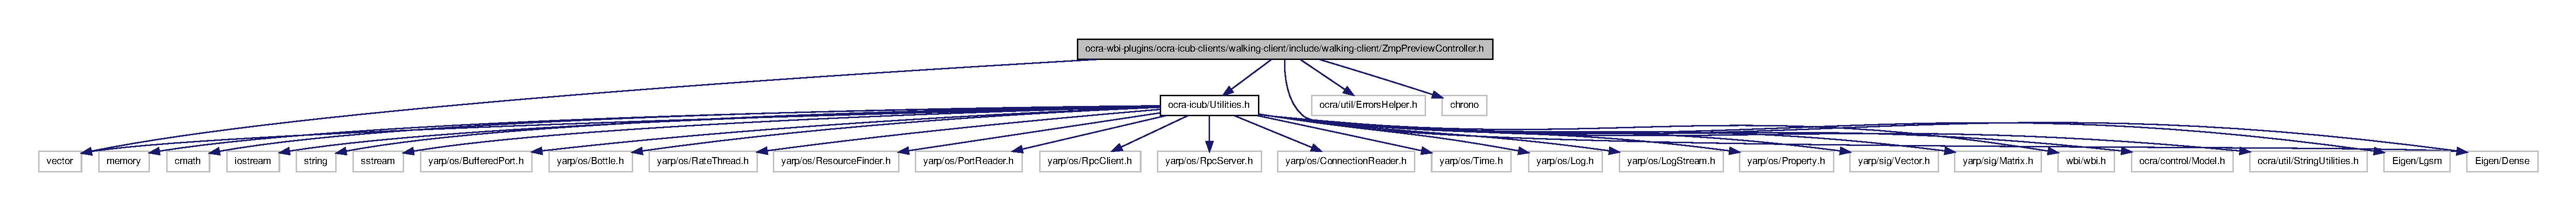
\includegraphics[width=350pt]{ZmpPreviewController_8h__incl}
\end{center}
\end{figure}
\-This graph shows which files directly or indirectly include this file\-:\nopagebreak
\begin{figure}[H]
\begin{center}
\leavevmode
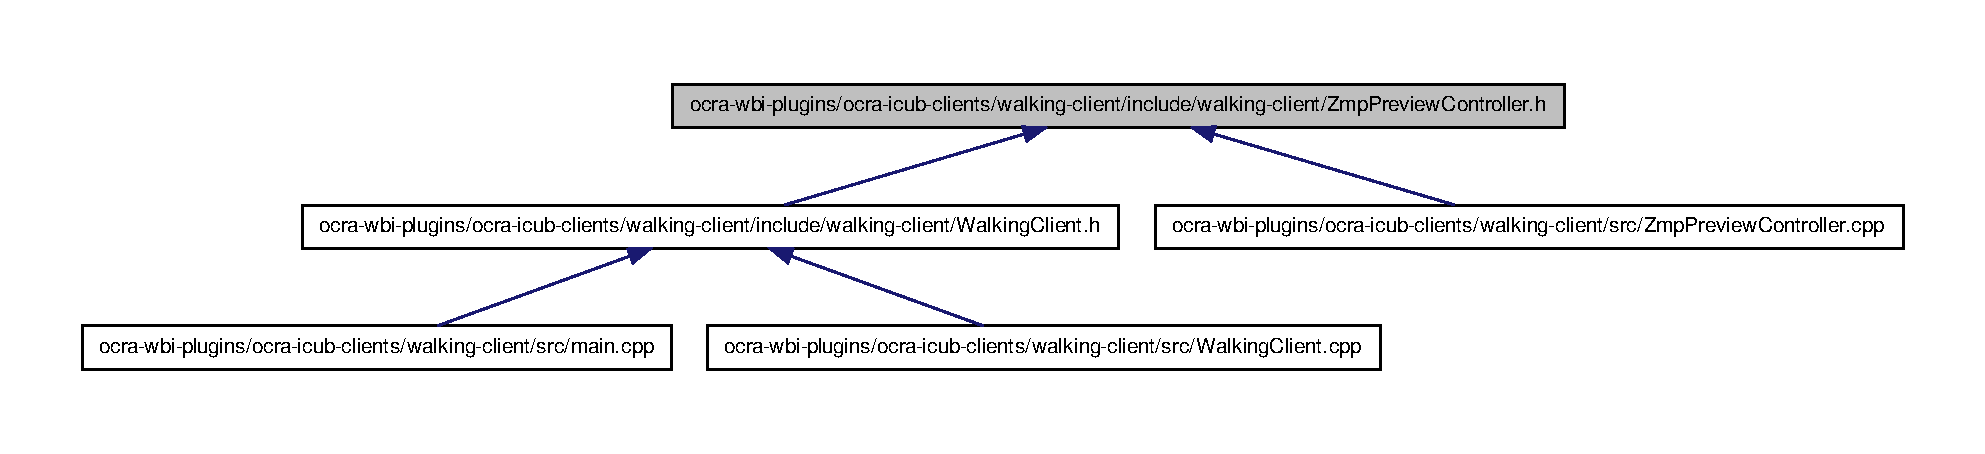
\includegraphics[width=350pt]{ZmpPreviewController_8h__dep__incl}
\end{center}
\end{figure}
\subsection*{\-Classes}
\begin{DoxyCompactItemize}
\item 
struct \hyperlink{structZmpPreviewParams}{\-Zmp\-Preview\-Params}
\item 
class \hyperlink{classZmpPreviewController}{\-Zmp\-Preview\-Controller}
\begin{DoxyCompactList}\small\item\em \-Implementes an extended \-Z\-M\-P preview controller as an unconstrained \-Q\-P problem. \end{DoxyCompactList}\end{DoxyCompactItemize}

\hypertarget{WalkingClient_8cpp}{\section{ocra-\/wbi-\/plugins/ocra-\/icub-\/clients/walking-\/client/src/\-Walking\-Client.cpp \-File \-Reference}
\label{WalkingClient_8cpp}\index{ocra-\/wbi-\/plugins/ocra-\/icub-\/clients/walking-\/client/src/\-Walking\-Client.\-cpp@{ocra-\/wbi-\/plugins/ocra-\/icub-\/clients/walking-\/client/src/\-Walking\-Client.\-cpp}}
}
{\ttfamily \#include \char`\"{}walking-\/client/\-Walking\-Client.\-h\char`\"{}}\*
\-Include dependency graph for \-Walking\-Client.\-cpp\-:\nopagebreak
\begin{figure}[H]
\begin{center}
\leavevmode
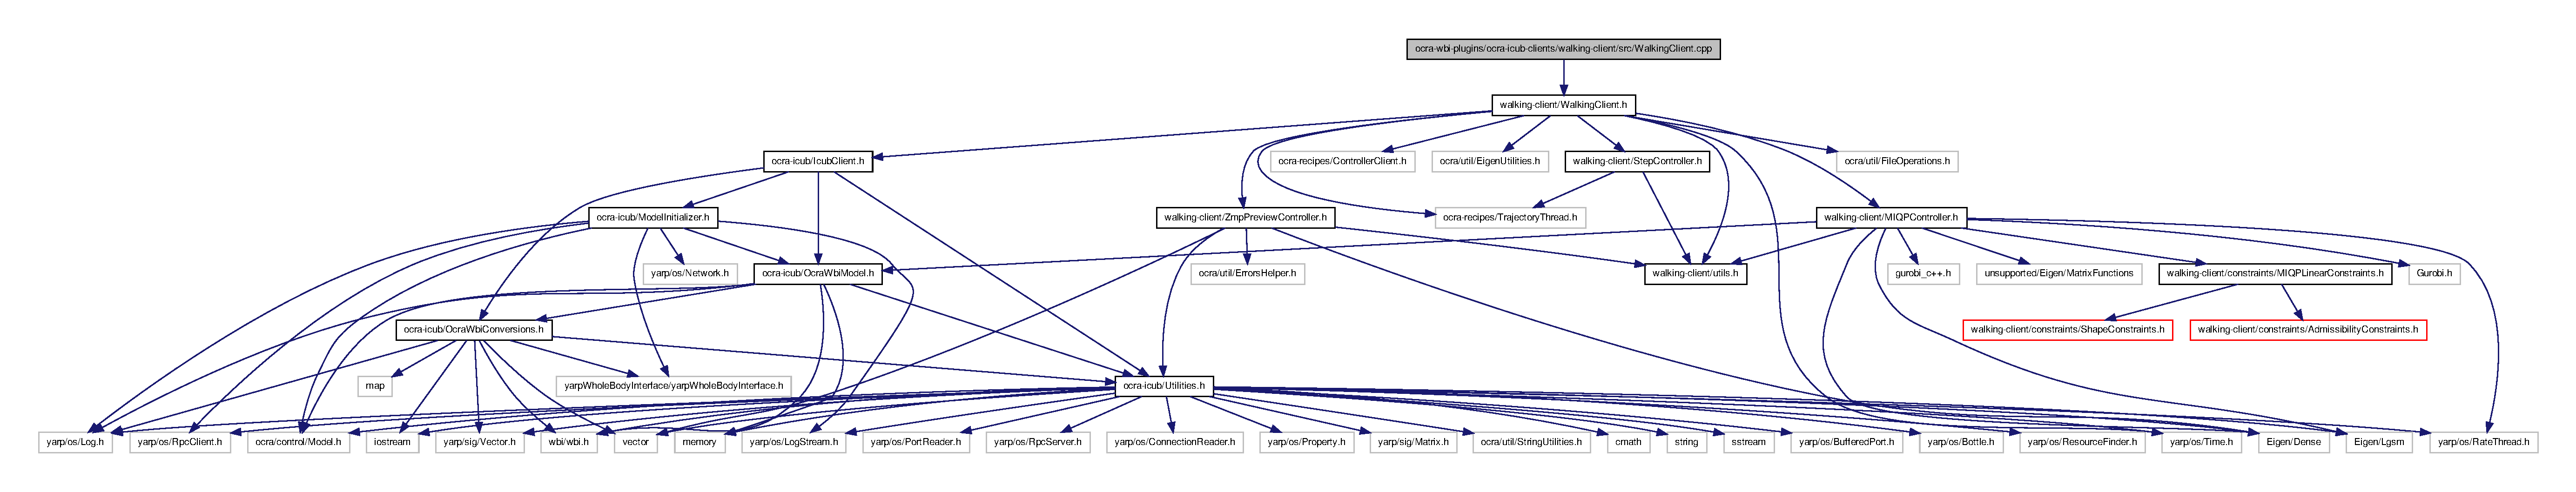
\includegraphics[width=350pt]{WalkingClient_8cpp__incl}
\end{center}
\end{figure}

\hypertarget{ZmpController_8cpp}{\section{ocra-\/wbi-\/plugins/ocra-\/icub-\/clients/walking-\/client/src/\-Zmp\-Controller.cpp \-File \-Reference}
\label{ZmpController_8cpp}\index{ocra-\/wbi-\/plugins/ocra-\/icub-\/clients/walking-\/client/src/\-Zmp\-Controller.\-cpp@{ocra-\/wbi-\/plugins/ocra-\/icub-\/clients/walking-\/client/src/\-Zmp\-Controller.\-cpp}}
}
{\ttfamily \#include \char`\"{}walking-\/client/\-Zmp\-Controller.\-h\char`\"{}}\*
\-Include dependency graph for \-Zmp\-Controller.\-cpp\-:\nopagebreak
\begin{figure}[H]
\begin{center}
\leavevmode
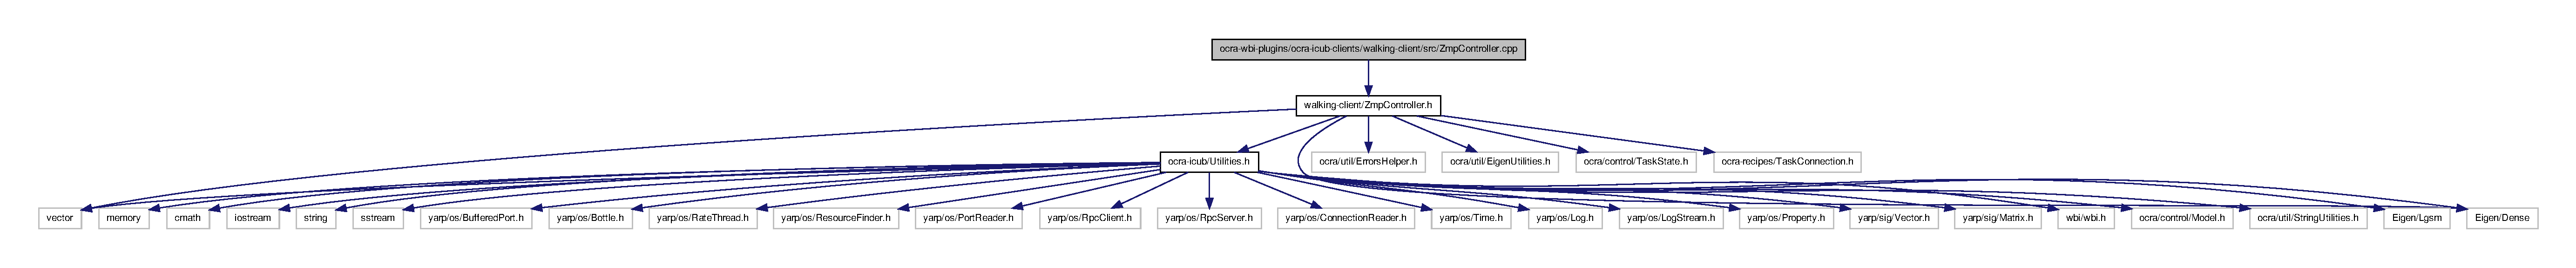
\includegraphics[width=350pt]{ZmpController_8cpp__incl}
\end{center}
\end{figure}

\hypertarget{ZmpPreviewController_8cpp}{\section{ocra-\/wbi-\/plugins/ocra-\/icub-\/clients/walking-\/client/src/\-Zmp\-Preview\-Controller.cpp \-File \-Reference}
\label{ZmpPreviewController_8cpp}\index{ocra-\/wbi-\/plugins/ocra-\/icub-\/clients/walking-\/client/src/\-Zmp\-Preview\-Controller.\-cpp@{ocra-\/wbi-\/plugins/ocra-\/icub-\/clients/walking-\/client/src/\-Zmp\-Preview\-Controller.\-cpp}}
}
{\ttfamily \#include \char`\"{}walking-\/client/\-Zmp\-Preview\-Controller.\-h\char`\"{}}\*
{\ttfamily \#include \char`\"{}unsupported/\-Eigen/\-Matrix\-Functions\char`\"{}}\*
\-Include dependency graph for \-Zmp\-Preview\-Controller.\-cpp\-:\nopagebreak
\begin{figure}[H]
\begin{center}
\leavevmode
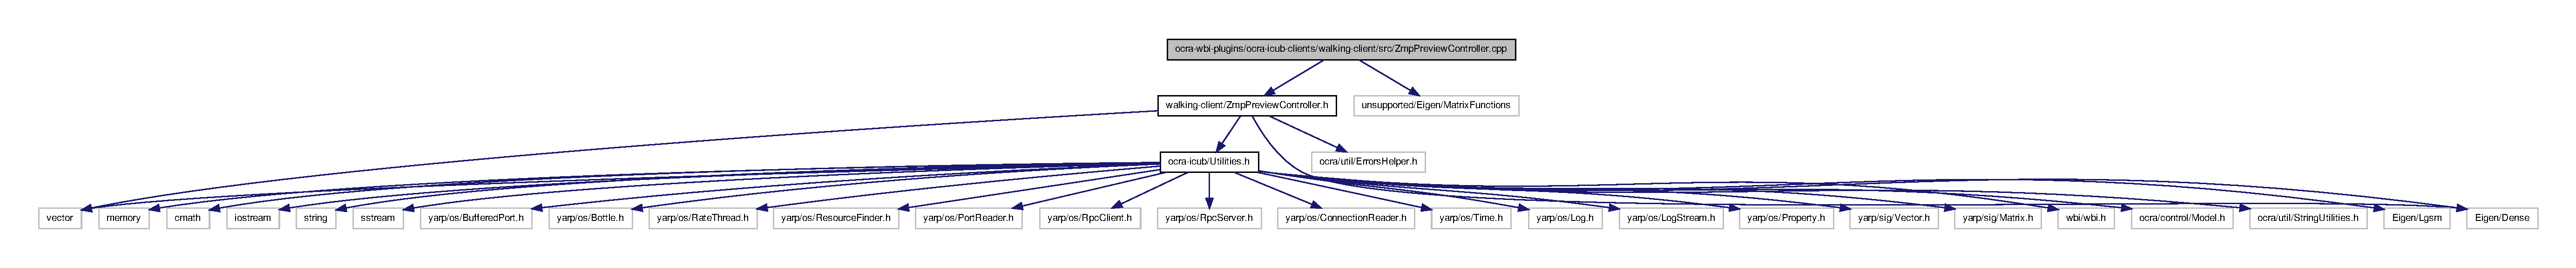
\includegraphics[width=350pt]{ZmpPreviewController_8cpp__incl}
\end{center}
\end{figure}

\hypertarget{IcubControllerServer_8h}{\section{ocra-\/wbi-\/plugins/ocra-\/icub-\/server/include/ocra-\/icub-\/server/\-Icub\-Controller\-Server.h \-File \-Reference}
\label{IcubControllerServer_8h}\index{ocra-\/wbi-\/plugins/ocra-\/icub-\/server/include/ocra-\/icub-\/server/\-Icub\-Controller\-Server.\-h@{ocra-\/wbi-\/plugins/ocra-\/icub-\/server/include/ocra-\/icub-\/server/\-Icub\-Controller\-Server.\-h}}
}
{\ttfamily \#include $<$wbi/wbi.\-h$>$}\*
{\ttfamily \#include $<$ocra-\/recipes/\-Controller\-Server.\-h$>$}\*
{\ttfamily \#include $<$\-Eigen/\-Dense$>$}\*
{\ttfamily \#include $<$ocra-\/icub/\-Ocra\-Wbi\-Model.\-h$>$}\*
{\ttfamily \#include $<$i\-Dyn\-Tree/\-Estimation/\-Simple\-Legged\-Odometry.\-h$>$}\*
{\ttfamily \#include $<$ocra/util/\-Errors\-Helper.\-h$>$}\*
\-Include dependency graph for \-Icub\-Controller\-Server.\-h\-:\nopagebreak
\begin{figure}[H]
\begin{center}
\leavevmode
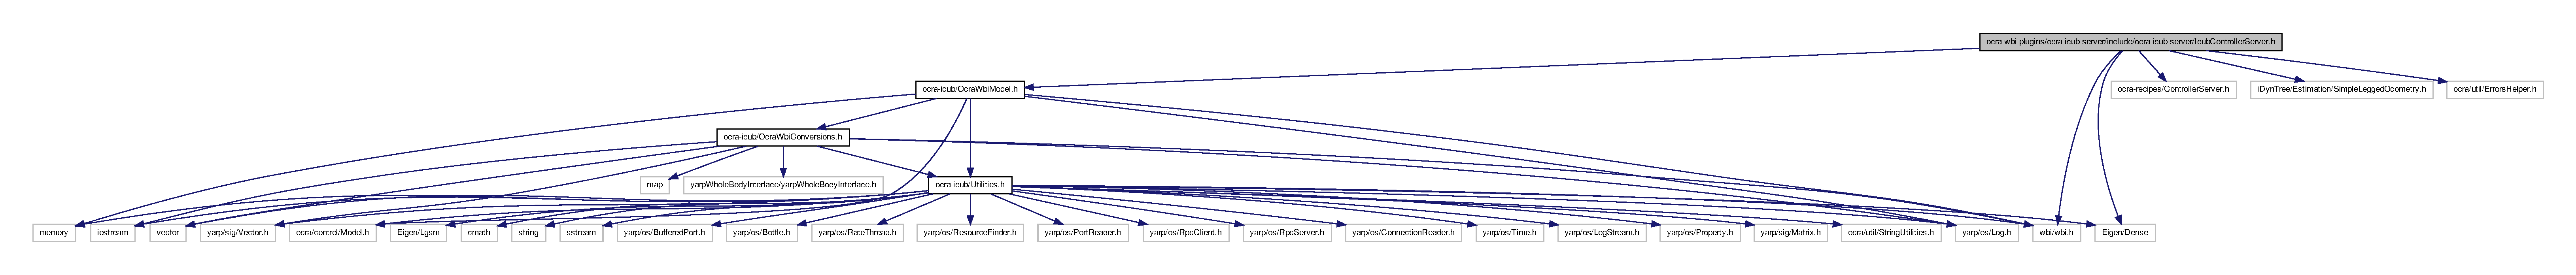
\includegraphics[width=350pt]{IcubControllerServer_8h__incl}
\end{center}
\end{figure}
\-This graph shows which files directly or indirectly include this file\-:\nopagebreak
\begin{figure}[H]
\begin{center}
\leavevmode
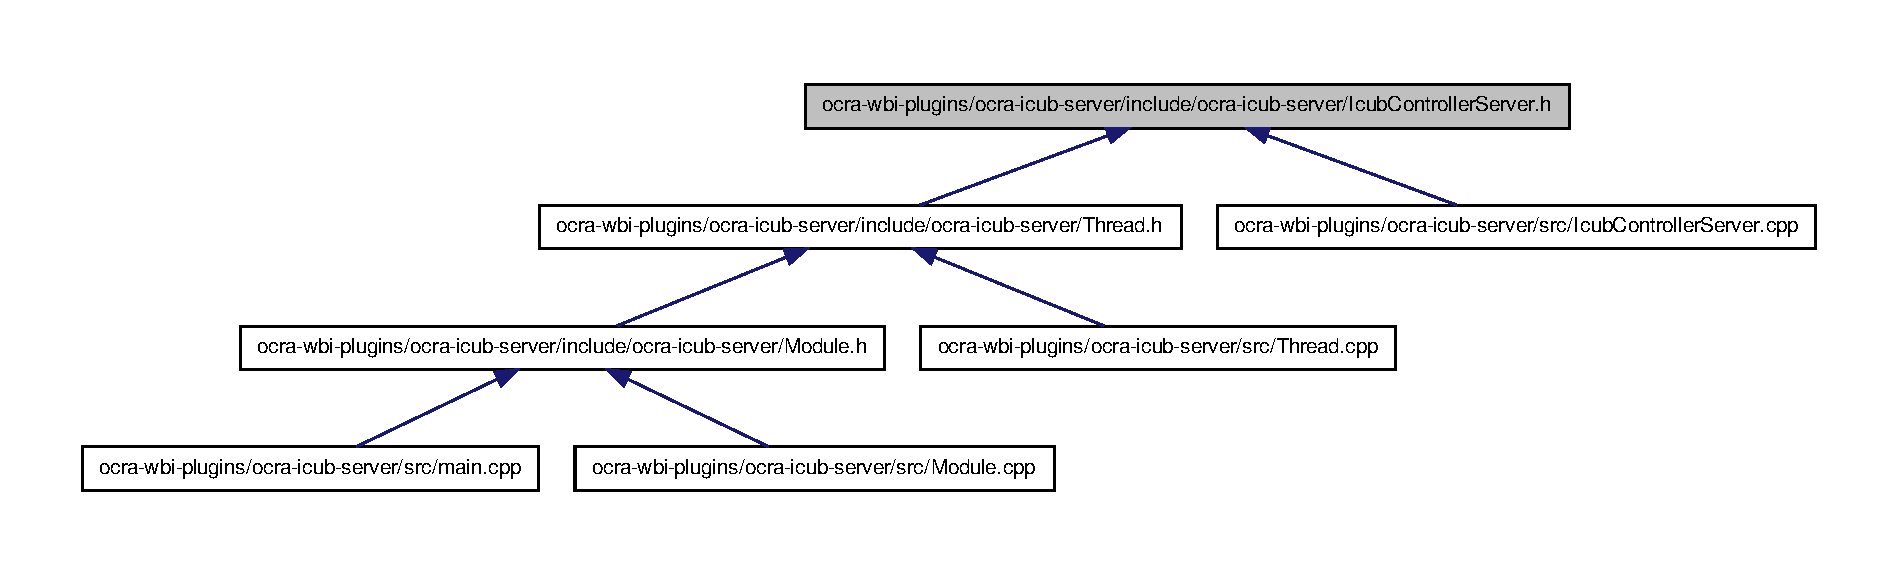
\includegraphics[width=350pt]{IcubControllerServer_8h__dep__incl}
\end{center}
\end{figure}
\subsection*{\-Classes}
\begin{DoxyCompactItemize}
\item 
class \hyperlink{classIcubControllerServer}{\-Icub\-Controller\-Server}
\end{DoxyCompactItemize}

\hypertarget{Module_8h}{\section{ocra-\/wbi-\/plugins/ocra-\/icub-\/server/include/ocra-\/icub-\/server/\-Module.h \-File \-Reference}
\label{Module_8h}\index{ocra-\/wbi-\/plugins/ocra-\/icub-\/server/include/ocra-\/icub-\/server/\-Module.\-h@{ocra-\/wbi-\/plugins/ocra-\/icub-\/server/include/ocra-\/icub-\/server/\-Module.\-h}}
}


\hyperlink{classModule}{\-Module} class for the controller server.  


{\ttfamily \#include $<$iostream$>$}\*
{\ttfamily \#include $<$memory$>$}\*
{\ttfamily \#include $<$algorithm$>$}\*
{\ttfamily \#include $<$locale$>$}\*
{\ttfamily \#include $<$yarp/os/\-R\-F\-Module.\-h$>$}\*
{\ttfamily \#include $<$yarp\-Whole\-Body\-Interface/yarp\-Whole\-Body\-Interface.\-h$>$}\*
{\ttfamily \#include \char`\"{}ocra-\/icub-\/server/\-Thread.\-h\char`\"{}}\*
{\ttfamily \#include \char`\"{}ocra-\/icub/\-Utilities.\-h\char`\"{}}\*
\-Include dependency graph for \-Module.\-h\-:\nopagebreak
\begin{figure}[H]
\begin{center}
\leavevmode
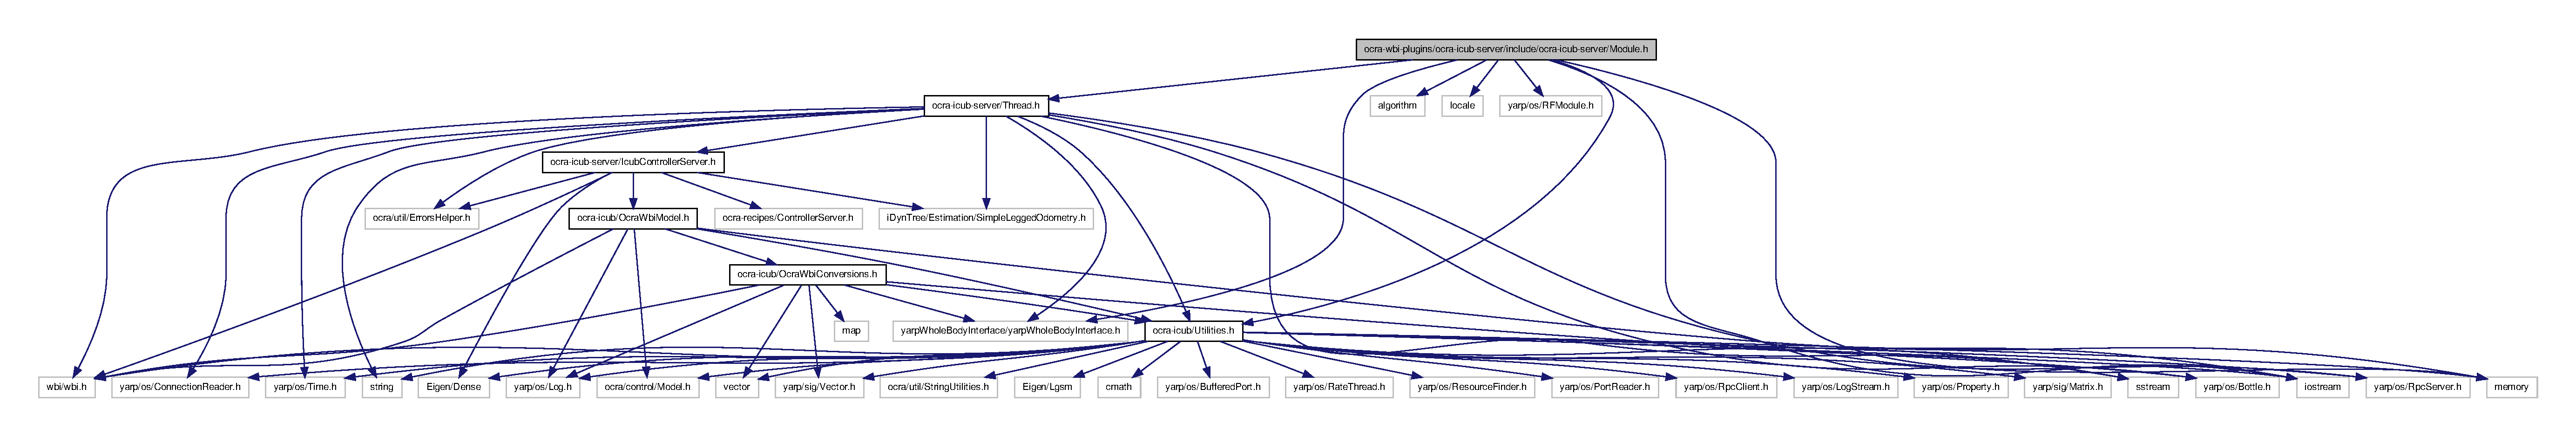
\includegraphics[width=350pt]{Module_8h__incl}
\end{center}
\end{figure}
\-This graph shows which files directly or indirectly include this file\-:\nopagebreak
\begin{figure}[H]
\begin{center}
\leavevmode
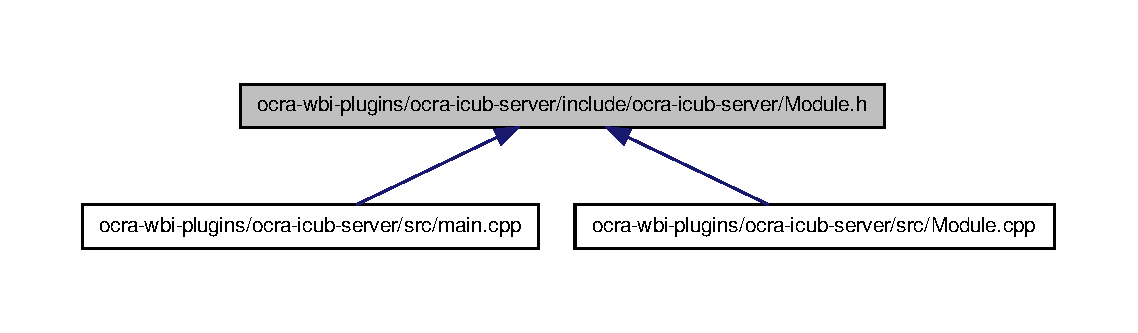
\includegraphics[width=350pt]{Module_8h__dep__incl}
\end{center}
\end{figure}
\subsection*{\-Classes}
\begin{DoxyCompactItemize}
\item 
class \hyperlink{classModule}{\-Module}
\begin{DoxyCompactList}\small\item\em \-The controller module which launches the controller thread. \end{DoxyCompactList}\end{DoxyCompactItemize}


\subsection{\-Detailed \-Description}
\hyperlink{classModule}{\-Module} class for the controller server. \begin{DoxyAuthor}{\-Author}
\mbox{[}\-Ryan \-Lober\mbox{]}(\href{http://www.ryanlober.com}{\tt http\-://www.\-ryanlober.\-com}) 

\mbox{[}\-Antoine \-Hoarau\mbox{]}(\href{http://ahoarau.github.io}{\tt http\-://ahoarau.\-github.\-io}) 
\end{DoxyAuthor}
\begin{DoxyDate}{\-Date}
\-Feb 2016 
\end{DoxyDate}
\begin{DoxyCopyright}{\-Copyright}
\-G\-N\-U \-General \-Public \-License. 
\end{DoxyCopyright}

\hypertarget{Thread_8h}{\section{ocra-\/wbi-\/plugins/ocra-\/icub-\/server/include/ocra-\/icub-\/server/\-Thread.h \-File \-Reference}
\label{Thread_8h}\index{ocra-\/wbi-\/plugins/ocra-\/icub-\/server/include/ocra-\/icub-\/server/\-Thread.\-h@{ocra-\/wbi-\/plugins/ocra-\/icub-\/server/include/ocra-\/icub-\/server/\-Thread.\-h}}
}


\-The thread class for the controller server.  


{\ttfamily \#include $<$yarp\-Whole\-Body\-Interface/yarp\-Whole\-Body\-Interface.\-h$>$}\*
{\ttfamily \#include $<$wbi/wbi.\-h$>$}\*
{\ttfamily \#include $<$ocra-\/icub-\/server/\-Icub\-Controller\-Server.\-h$>$}\*
{\ttfamily \#include $<$ocra-\/icub/\-Utilities.\-h$>$}\*
{\ttfamily \#include $<$ocra/util/\-Errors\-Helper.\-h$>$}\*
{\ttfamily \#include $<$yarp/os/\-Bottle.\-h$>$}\*
{\ttfamily \#include $<$yarp/os/\-Rpc\-Server.\-h$>$}\*
{\ttfamily \#include $<$yarp/os/\-Connection\-Reader.\-h$>$}\*
{\ttfamily \#include $<$yarp/os/\-Time.\-h$>$}\*
{\ttfamily \#include $<$sstream$>$}\*
{\ttfamily \#include $<$string$>$}\*
{\ttfamily \#include $<$i\-Dyn\-Tree/\-Estimation/\-Simple\-Legged\-Odometry.\-h$>$}\*
\-Include dependency graph for \-Thread.\-h\-:
\nopagebreak
\begin{figure}[H]
\begin{center}
\leavevmode
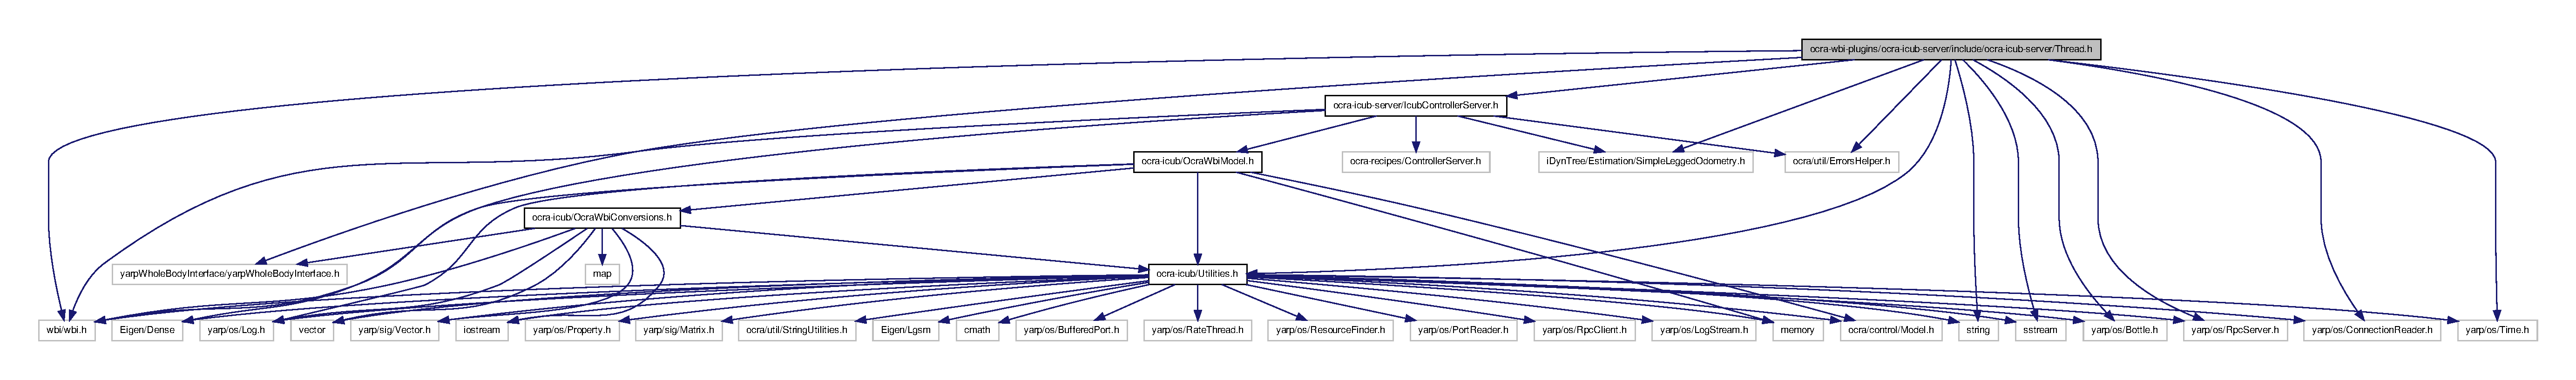
\includegraphics[width=350pt]{Thread_8h__incl}
\end{center}
\end{figure}
\-This graph shows which files directly or indirectly include this file\-:
\nopagebreak
\begin{figure}[H]
\begin{center}
\leavevmode
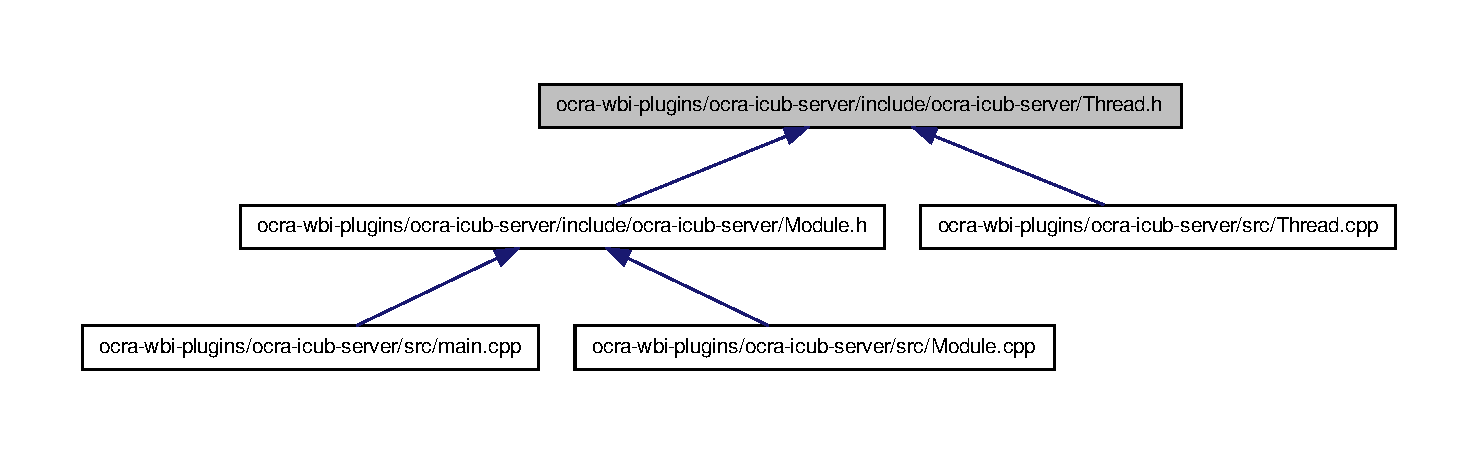
\includegraphics[width=350pt]{Thread_8h__dep__incl}
\end{center}
\end{figure}
\subsection*{\-Classes}
\begin{DoxyCompactItemize}
\item 
class \hyperlink{classOcraControllerOptions}{\-Ocra\-Controller\-Options}
\item 
class \hyperlink{classThread}{\-Thread}
\begin{DoxyCompactList}\small\item\em \-The meat and potatoes of the controller server. \end{DoxyCompactList}\item 
class \hyperlink{classThread_1_1ControllerRpcServerCallback}{\-Thread\-::\-Controller\-Rpc\-Server\-Callback}
\begin{DoxyCompactList}\small\item\em \-A callback function which binds the rpc server port opened in the contoller server module to the controller thread's parsing function. \end{DoxyCompactList}\item 
class \hyperlink{classThread_1_1DebugRpcServerCallback}{\-Thread\-::\-Debug\-Rpc\-Server\-Callback}
\begin{DoxyCompactList}\small\item\em \-A callback function which binds the rpc server port opened in the contoller server module to the controller thread's parsing function. \end{DoxyCompactList}\end{DoxyCompactItemize}


\subsection{\-Detailed \-Description}
\-The thread class for the controller server. \begin{DoxyAuthor}{\-Author}
\mbox{[}\-Ryan \-Lober\mbox{]}(\href{http://www.ryanlober.com}{\tt http\-://www.\-ryanlober.\-com}) 

\mbox{[}\-Antoine \-Hoarau\mbox{]}(\href{http://ahoarau.github.io}{\tt http\-://ahoarau.\-github.\-io}) 
\end{DoxyAuthor}
\begin{DoxyDate}{\-Date}
\-Feb 2016 
\end{DoxyDate}
\begin{DoxyCopyright}{\-Copyright}
\-G\-N\-U \-General \-Public \-License. 
\end{DoxyCopyright}

\hypertarget{IcubControllerServer_8cpp}{\section{ocra-\/wbi-\/plugins/ocra-\/icub-\/server/src/\-Icub\-Controller\-Server.cpp \-File \-Reference}
\label{IcubControllerServer_8cpp}\index{ocra-\/wbi-\/plugins/ocra-\/icub-\/server/src/\-Icub\-Controller\-Server.\-cpp@{ocra-\/wbi-\/plugins/ocra-\/icub-\/server/src/\-Icub\-Controller\-Server.\-cpp}}
}
{\ttfamily \#include $<$ocra-\/icub-\/server/\-Icub\-Controller\-Server.\-h$>$}\*
\-Include dependency graph for \-Icub\-Controller\-Server.\-cpp\-:\nopagebreak
\begin{figure}[H]
\begin{center}
\leavevmode
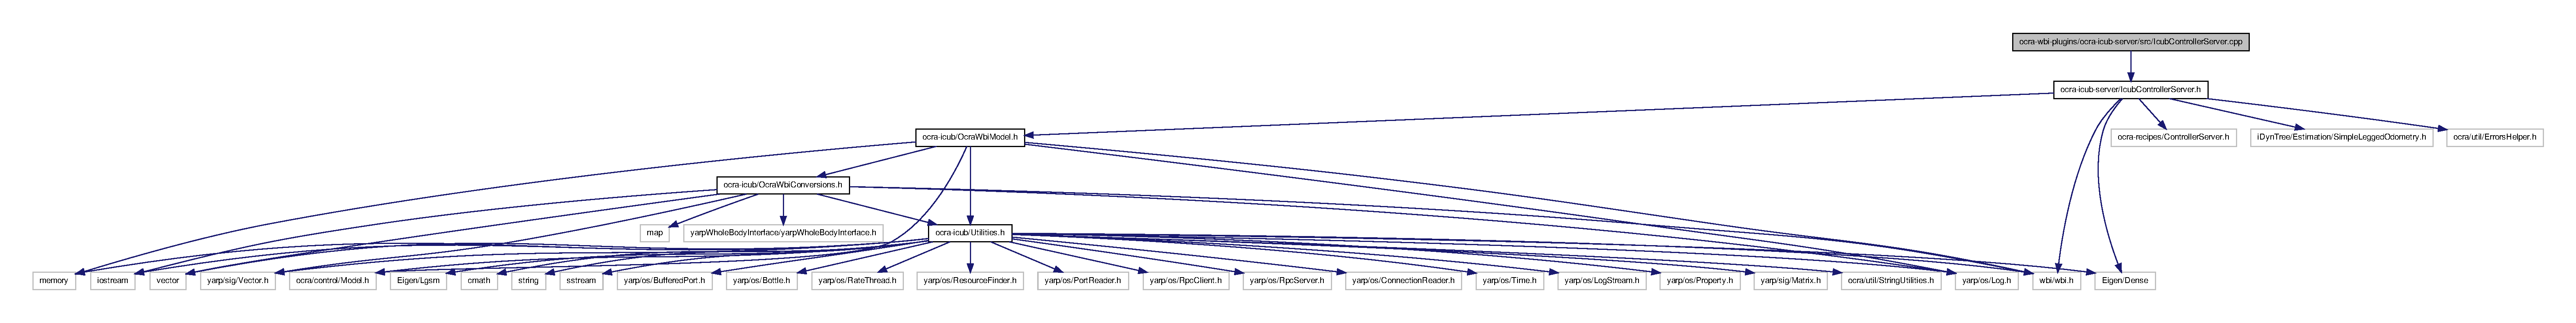
\includegraphics[width=350pt]{IcubControllerServer_8cpp__incl}
\end{center}
\end{figure}

\hypertarget{ocra-icub-server_2src_2main_8cpp}{\section{ocra-\/wbi-\/plugins/ocra-\/icub-\/server/src/main.cpp \-File \-Reference}
\label{ocra-icub-server_2src_2main_8cpp}\index{ocra-\/wbi-\/plugins/ocra-\/icub-\/server/src/main.\-cpp@{ocra-\/wbi-\/plugins/ocra-\/icub-\/server/src/main.\-cpp}}
}
{\ttfamily \#include $<$yarp/os/\-Resource\-Finder.\-h$>$}\*
{\ttfamily \#include $<$yarp/os/\-Network.\-h$>$}\*
{\ttfamily \#include $<$yarp/os/\-Log.\-h$>$}\*
{\ttfamily \#include $<$ocra-\/icub-\/server/\-Module.\-h$>$}\*
\-Include dependency graph for main.\-cpp\-:
\nopagebreak
\begin{figure}[H]
\begin{center}
\leavevmode
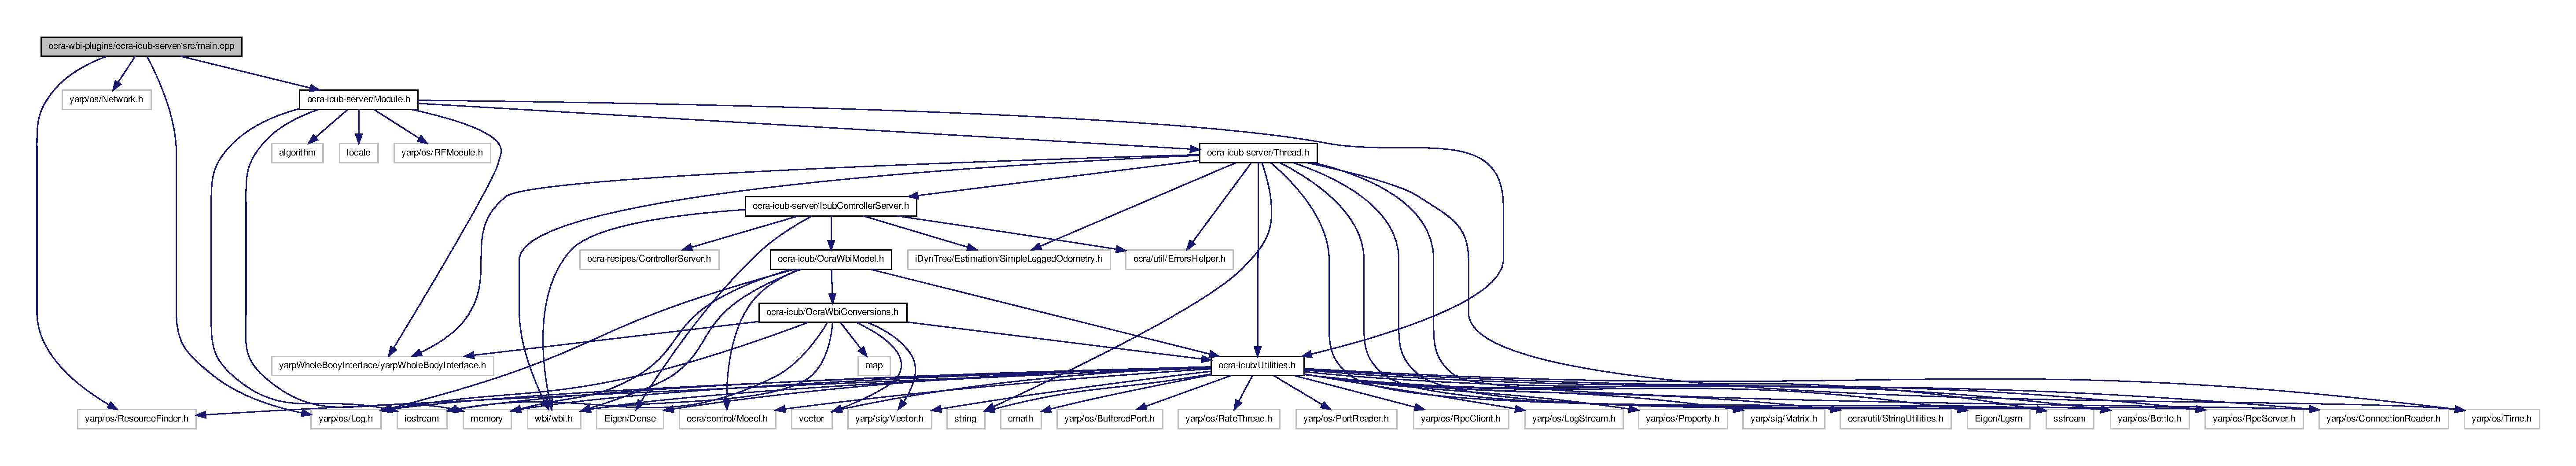
\includegraphics[width=350pt]{ocra-icub-server_2src_2main_8cpp__incl}
\end{center}
\end{figure}
\subsection*{\-Defines}
\begin{DoxyCompactItemize}
\item 
\#define \hyperlink{ocra-icub-server_2src_2main_8cpp_aacf7b13861a4ce37b8dec1979eb6450c}{\-D\-E\-F\-A\-U\-L\-T\-\_\-\-Y\-A\-R\-P\-\_\-\-C\-O\-N\-T\-E\-X\-T}~\char`\"{}ocra-\/icub-\/server\char`\"{}
\end{DoxyCompactItemize}
\subsection*{\-Functions}
\begin{DoxyCompactItemize}
\item 
int \hyperlink{ocra-icub-server_2src_2main_8cpp_a0ddf1224851353fc92bfbff6f499fa97}{main} (int argc, char $\ast$argv\mbox{[}$\,$\mbox{]})
\end{DoxyCompactItemize}


\subsection{\-Define \-Documentation}
\hypertarget{ocra-icub-server_2src_2main_8cpp_aacf7b13861a4ce37b8dec1979eb6450c}{\index{ocra-\/icub-\/server/src/main.\-cpp@{ocra-\/icub-\/server/src/main.\-cpp}!\-D\-E\-F\-A\-U\-L\-T\-\_\-\-Y\-A\-R\-P\-\_\-\-C\-O\-N\-T\-E\-X\-T@{\-D\-E\-F\-A\-U\-L\-T\-\_\-\-Y\-A\-R\-P\-\_\-\-C\-O\-N\-T\-E\-X\-T}}
\index{\-D\-E\-F\-A\-U\-L\-T\-\_\-\-Y\-A\-R\-P\-\_\-\-C\-O\-N\-T\-E\-X\-T@{\-D\-E\-F\-A\-U\-L\-T\-\_\-\-Y\-A\-R\-P\-\_\-\-C\-O\-N\-T\-E\-X\-T}!ocra-icub-server/src/main.cpp@{ocra-\/icub-\/server/src/main.\-cpp}}
\subsubsection[{\-D\-E\-F\-A\-U\-L\-T\-\_\-\-Y\-A\-R\-P\-\_\-\-C\-O\-N\-T\-E\-X\-T}]{\setlength{\rightskip}{0pt plus 5cm}\#define {\bf \-D\-E\-F\-A\-U\-L\-T\-\_\-\-Y\-A\-R\-P\-\_\-\-C\-O\-N\-T\-E\-X\-T}~\char`\"{}ocra-\/icub-\/server\char`\"{}}}\label{ocra-icub-server_2src_2main_8cpp_aacf7b13861a4ce37b8dec1979eb6450c}


\subsection{\-Function \-Documentation}
\hypertarget{ocra-icub-server_2src_2main_8cpp_a0ddf1224851353fc92bfbff6f499fa97}{\index{ocra-\/icub-\/server/src/main.\-cpp@{ocra-\/icub-\/server/src/main.\-cpp}!main@{main}}
\index{main@{main}!ocra-icub-server/src/main.cpp@{ocra-\/icub-\/server/src/main.\-cpp}}
\subsubsection[{main}]{\setlength{\rightskip}{0pt plus 5cm}int {\bf main} (
\begin{DoxyParamCaption}
\item[{int}]{argc, }
\item[{char $\ast$}]{argv\mbox{[}$\,$\mbox{]}}
\end{DoxyParamCaption}
)}}\label{ocra-icub-server_2src_2main_8cpp_a0ddf1224851353fc92bfbff6f499fa97}

\hypertarget{ocra-icub-clients_2sitting-demo_2src_2main_8cpp}{\section{ocra-\/wbi-\/plugins/ocra-\/icub-\/clients/sitting-\/demo/src/main.cpp \-File \-Reference}
\label{ocra-icub-clients_2sitting-demo_2src_2main_8cpp}\index{ocra-\/wbi-\/plugins/ocra-\/icub-\/clients/sitting-\/demo/src/main.\-cpp@{ocra-\/wbi-\/plugins/ocra-\/icub-\/clients/sitting-\/demo/src/main.\-cpp}}
}
{\ttfamily \#include $<$yarp/os/\-Resource\-Finder.\-h$>$}\*
{\ttfamily \#include $<$yarp/os/\-Network.\-h$>$}\*
{\ttfamily \#include $<$yarp/os/\-Log.\-h$>$}\*
{\ttfamily \#include $<$yarp/os/\-Log\-Stream.\-h$>$}\*
{\ttfamily \#include $<$yarp/os/\-Time.\-h$>$}\*
{\ttfamily \#include $<$ocra-\/icub/\-Icub\-Client.\-h$>$}\*
{\ttfamily \#include $<$ocra-\/recipes/\-Controller\-Client.\-h$>$}\*
{\ttfamily \#include $<$ocra-\/recipes/\-Client\-Manager.\-h$>$}\*
{\ttfamily \#include \char`\"{}sitting-\/demo/\-Sitting\-Demo\-Client.\-h\char`\"{}}\*
\-Include dependency graph for main.\-cpp\-:\nopagebreak
\begin{figure}[H]
\begin{center}
\leavevmode
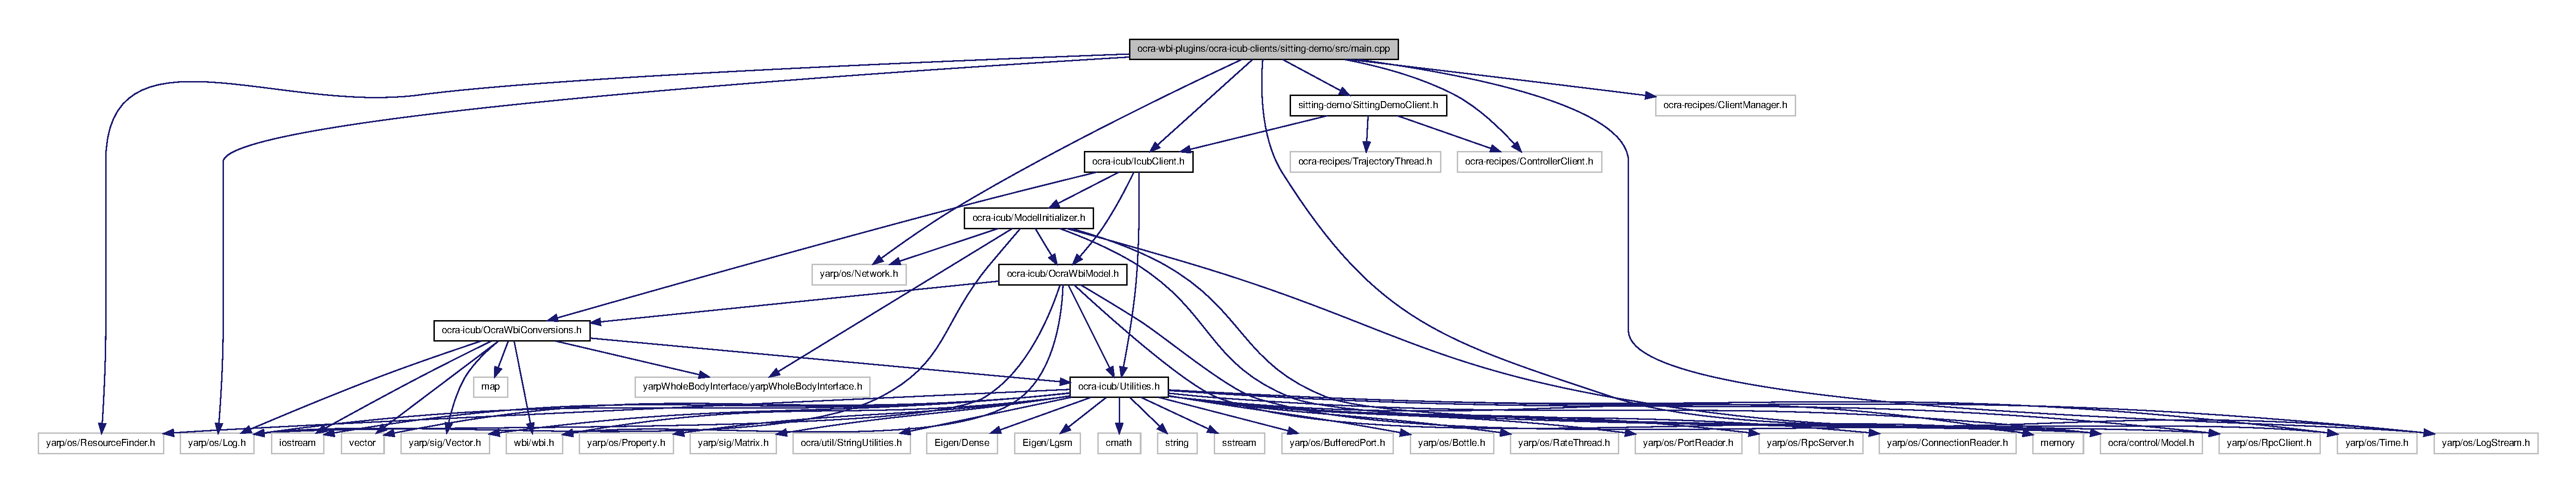
\includegraphics[width=350pt]{ocra-icub-clients_2sitting-demo_2src_2main_8cpp__incl}
\end{center}
\end{figure}
\subsection*{\-Functions}
\begin{DoxyCompactItemize}
\item 
int \hyperlink{ocra-icub-clients_2sitting-demo_2src_2main_8cpp_a0ddf1224851353fc92bfbff6f499fa97}{main} (int argc, char $\ast$argv\mbox{[}$\,$\mbox{]})
\end{DoxyCompactItemize}


\subsection{\-Function \-Documentation}
\hypertarget{ocra-icub-clients_2sitting-demo_2src_2main_8cpp_a0ddf1224851353fc92bfbff6f499fa97}{\index{ocra-\/icub-\/clients/sitting-\/demo/src/main.\-cpp@{ocra-\/icub-\/clients/sitting-\/demo/src/main.\-cpp}!main@{main}}
\index{main@{main}!ocra-icub-clients/sitting-demo/src/main.cpp@{ocra-\/icub-\/clients/sitting-\/demo/src/main.\-cpp}}
\subsubsection[{main}]{\setlength{\rightskip}{0pt plus 5cm}int {\bf main} (
\begin{DoxyParamCaption}
\item[{int}]{argc, }
\item[{char $\ast$}]{argv\mbox{[}$\,$\mbox{]}}
\end{DoxyParamCaption}
)}}\label{ocra-icub-clients_2sitting-demo_2src_2main_8cpp_a0ddf1224851353fc92bfbff6f499fa97}
ile main.\-cpp rief

uthor \mbox{[}\-Your \-Name\mbox{]}(url of your github site) \begin{DoxyDate}{\-Date}
\mbox{[}date\mbox{]} 
\end{DoxyDate}
\begin{DoxyCopyright}{\-Copyright}
\-G\-N\-U \-General \-Public \-License. 
\end{DoxyCopyright}

\hypertarget{ocra-icub-clients_2standing-demo_2src_2main_8cpp}{\section{ocra-\/wbi-\/plugins/ocra-\/icub-\/clients/standing-\/demo/src/main.cpp \-File \-Reference}
\label{ocra-icub-clients_2standing-demo_2src_2main_8cpp}\index{ocra-\/wbi-\/plugins/ocra-\/icub-\/clients/standing-\/demo/src/main.\-cpp@{ocra-\/wbi-\/plugins/ocra-\/icub-\/clients/standing-\/demo/src/main.\-cpp}}
}
{\ttfamily \#include $<$yarp/os/\-Resource\-Finder.\-h$>$}\*
{\ttfamily \#include $<$yarp/os/\-Network.\-h$>$}\*
{\ttfamily \#include $<$yarp/os/\-Log.\-h$>$}\*
{\ttfamily \#include $<$yarp/os/\-Log\-Stream.\-h$>$}\*
{\ttfamily \#include $<$yarp/os/\-Time.\-h$>$}\*
{\ttfamily \#include $<$ocra-\/icub/\-Icub\-Client.\-h$>$}\*
{\ttfamily \#include $<$ocra-\/recipes/\-Controller\-Client.\-h$>$}\*
{\ttfamily \#include $<$ocra-\/recipes/\-Client\-Manager.\-h$>$}\*
{\ttfamily \#include \char`\"{}standing-\/demo/\-Standing\-Demo\-Client.\-h\char`\"{}}\*
\-Include dependency graph for main.\-cpp\-:\nopagebreak
\begin{figure}[H]
\begin{center}
\leavevmode
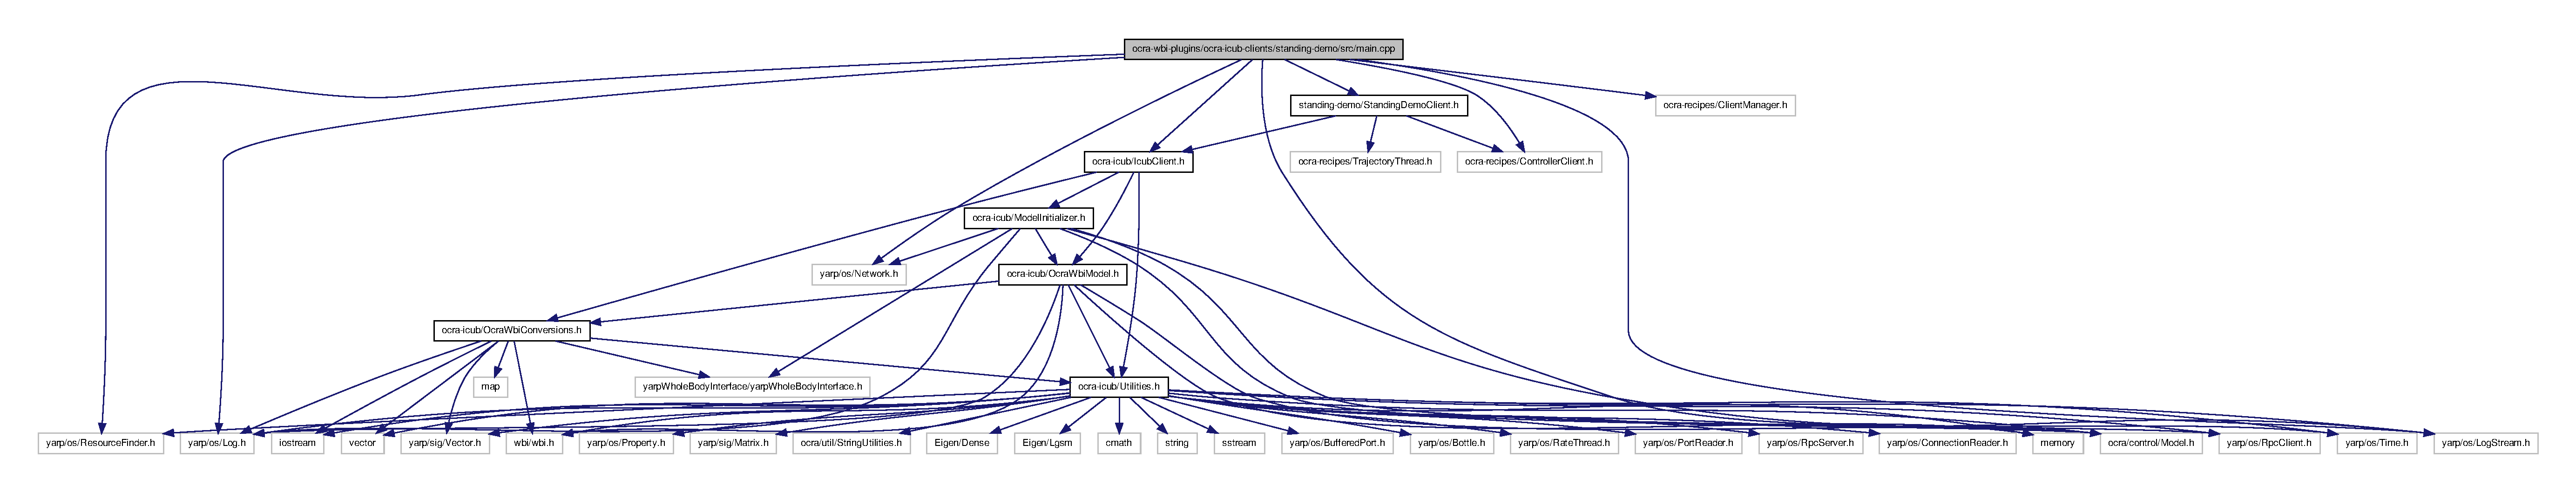
\includegraphics[width=350pt]{ocra-icub-clients_2standing-demo_2src_2main_8cpp__incl}
\end{center}
\end{figure}
\subsection*{\-Functions}
\begin{DoxyCompactItemize}
\item 
int \hyperlink{ocra-icub-clients_2standing-demo_2src_2main_8cpp_a0ddf1224851353fc92bfbff6f499fa97}{main} (int argc, char $\ast$argv\mbox{[}$\,$\mbox{]})
\end{DoxyCompactItemize}


\subsection{\-Function \-Documentation}
\hypertarget{ocra-icub-clients_2standing-demo_2src_2main_8cpp_a0ddf1224851353fc92bfbff6f499fa97}{\index{ocra-\/icub-\/clients/standing-\/demo/src/main.\-cpp@{ocra-\/icub-\/clients/standing-\/demo/src/main.\-cpp}!main@{main}}
\index{main@{main}!ocra-icub-clients/standing-demo/src/main.cpp@{ocra-\/icub-\/clients/standing-\/demo/src/main.\-cpp}}
\subsubsection[{main}]{\setlength{\rightskip}{0pt plus 5cm}int {\bf main} (
\begin{DoxyParamCaption}
\item[{int}]{argc, }
\item[{char $\ast$}]{argv\mbox{[}$\,$\mbox{]}}
\end{DoxyParamCaption}
)}}\label{ocra-icub-clients_2standing-demo_2src_2main_8cpp_a0ddf1224851353fc92bfbff6f499fa97}
ile main.\-cpp rief

uthor \mbox{[}\-Your \-Name\mbox{]}(url of your github site) \begin{DoxyDate}{\-Date}
\mbox{[}date\mbox{]} 
\end{DoxyDate}
\begin{DoxyCopyright}{\-Copyright}
\-G\-N\-U \-General \-Public \-License. 
\end{DoxyCopyright}

\hypertarget{ocra-icub-clients_2walking-client_2src_2main_8cpp}{\section{ocra-\/wbi-\/plugins/ocra-\/icub-\/clients/walking-\/client/src/main.cpp \-File \-Reference}
\label{ocra-icub-clients_2walking-client_2src_2main_8cpp}\index{ocra-\/wbi-\/plugins/ocra-\/icub-\/clients/walking-\/client/src/main.\-cpp@{ocra-\/wbi-\/plugins/ocra-\/icub-\/clients/walking-\/client/src/main.\-cpp}}
}
{\ttfamily \#include $<$yarp/os/\-Resource\-Finder.\-h$>$}\*
{\ttfamily \#include $<$yarp/os/\-Network.\-h$>$}\*
{\ttfamily \#include $<$yarp/os/\-Log.\-h$>$}\*
{\ttfamily \#include $<$yarp/os/\-Log\-Stream.\-h$>$}\*
{\ttfamily \#include $<$yarp/os/\-Time.\-h$>$}\*
{\ttfamily \#include $<$ocra-\/icub/\-Icub\-Client.\-h$>$}\*
{\ttfamily \#include $<$ocra-\/recipes/\-Controller\-Client.\-h$>$}\*
{\ttfamily \#include $<$ocra-\/recipes/\-Client\-Manager.\-h$>$}\*
{\ttfamily \#include \char`\"{}walking-\/client/\-Walking\-Client.\-h\char`\"{}}\*
\-Include dependency graph for main.\-cpp\-:
\nopagebreak
\begin{figure}[H]
\begin{center}
\leavevmode
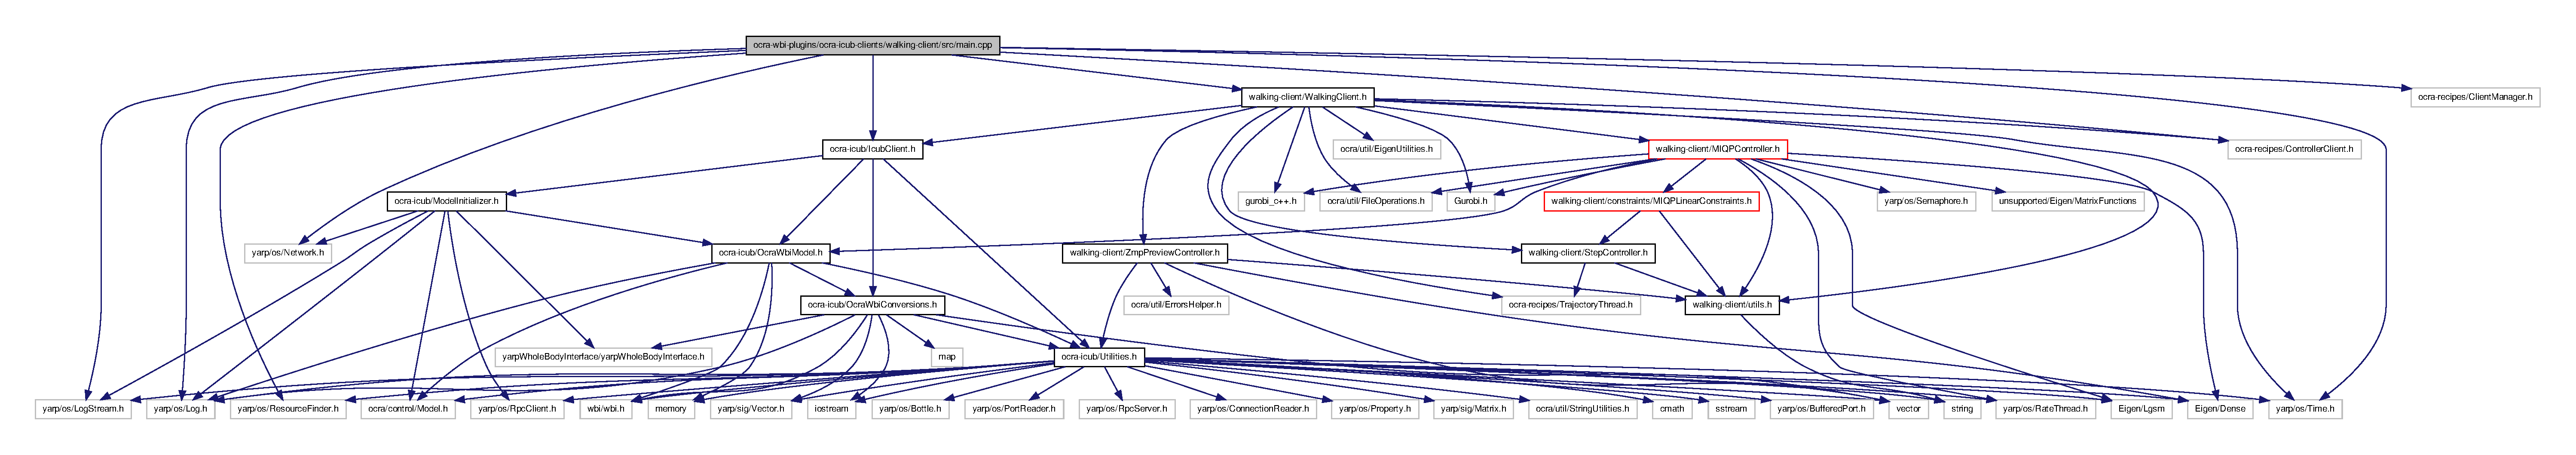
\includegraphics[width=350pt]{ocra-icub-clients_2walking-client_2src_2main_8cpp__incl}
\end{center}
\end{figure}
\subsection*{\-Functions}
\begin{DoxyCompactItemize}
\item 
int \hyperlink{ocra-icub-clients_2walking-client_2src_2main_8cpp_a0ddf1224851353fc92bfbff6f499fa97}{main} (int argc, char $\ast$argv\mbox{[}$\,$\mbox{]})
\end{DoxyCompactItemize}


\subsection{\-Function \-Documentation}
\hypertarget{ocra-icub-clients_2walking-client_2src_2main_8cpp_a0ddf1224851353fc92bfbff6f499fa97}{\index{ocra-\/icub-\/clients/walking-\/client/src/main.\-cpp@{ocra-\/icub-\/clients/walking-\/client/src/main.\-cpp}!main@{main}}
\index{main@{main}!ocra-icub-clients/walking-client/src/main.cpp@{ocra-\/icub-\/clients/walking-\/client/src/main.\-cpp}}
\subsubsection[{main}]{\setlength{\rightskip}{0pt plus 5cm}int {\bf main} (
\begin{DoxyParamCaption}
\item[{int}]{argc, }
\item[{char $\ast$}]{argv\mbox{[}$\,$\mbox{]}}
\end{DoxyParamCaption}
)}}\label{ocra-icub-clients_2walking-client_2src_2main_8cpp_a0ddf1224851353fc92bfbff6f499fa97}

\hypertarget{Module_8cpp}{\section{ocra-\/wbi-\/plugins/ocra-\/icub-\/server/src/\-Module.cpp \-File \-Reference}
\label{Module_8cpp}\index{ocra-\/wbi-\/plugins/ocra-\/icub-\/server/src/\-Module.\-cpp@{ocra-\/wbi-\/plugins/ocra-\/icub-\/server/src/\-Module.\-cpp}}
}
{\ttfamily \#include \char`\"{}ocra-\/icub-\/server/\-Module.\-h\char`\"{}}\*
\-Include dependency graph for \-Module.\-cpp\-:\nopagebreak
\begin{figure}[H]
\begin{center}
\leavevmode
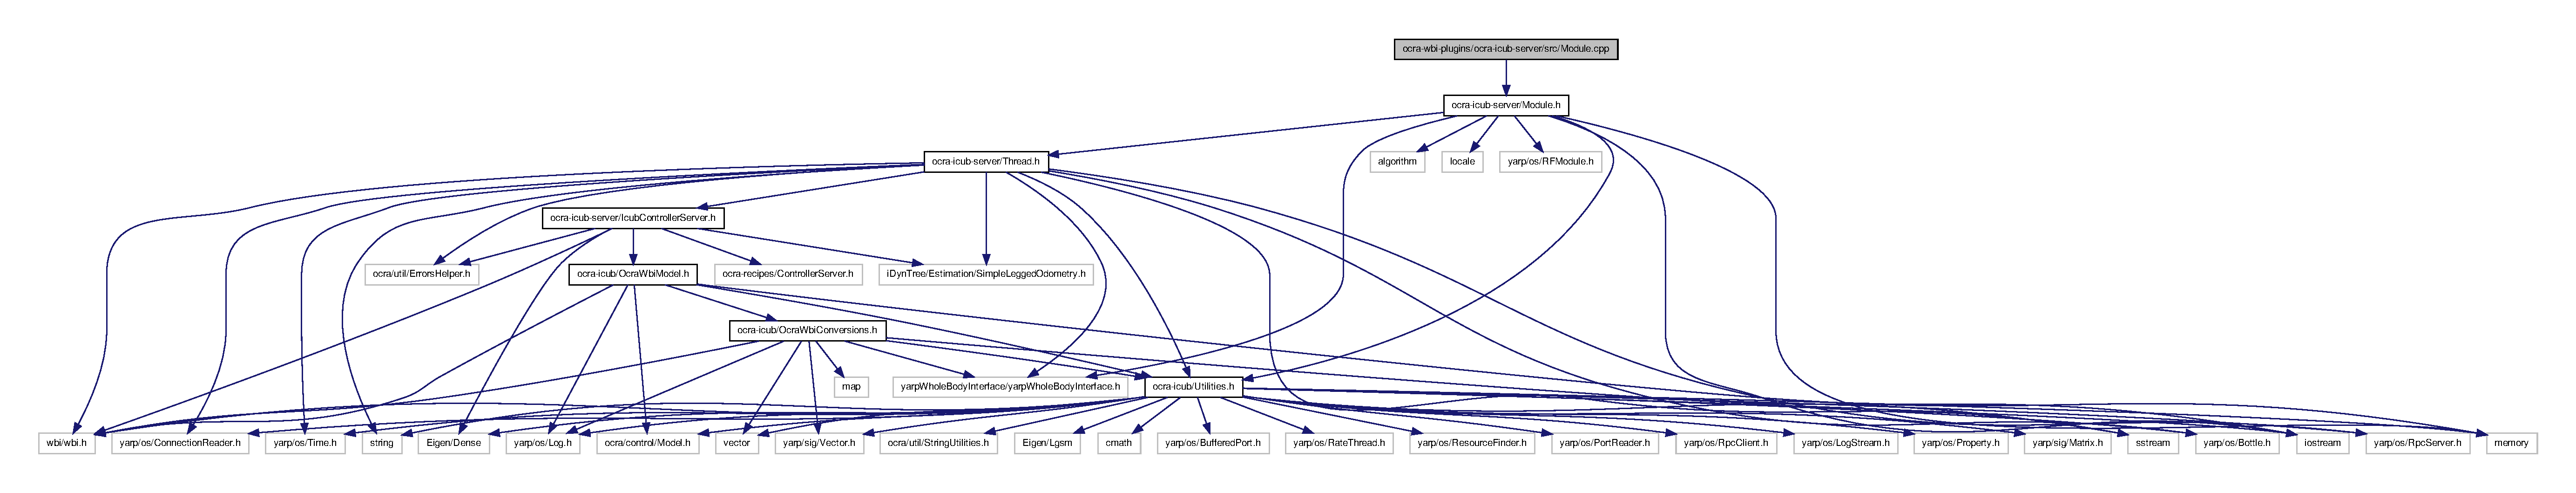
\includegraphics[width=350pt]{Module_8cpp__incl}
\end{center}
\end{figure}

\hypertarget{Thread_8cpp}{\section{ocra-\/wbi-\/plugins/ocra-\/icub-\/server/src/\-Thread.cpp \-File \-Reference}
\label{Thread_8cpp}\index{ocra-\/wbi-\/plugins/ocra-\/icub-\/server/src/\-Thread.\-cpp@{ocra-\/wbi-\/plugins/ocra-\/icub-\/server/src/\-Thread.\-cpp}}
}


\-The thread class for the controller server.  


{\ttfamily \#include \char`\"{}ocra-\/icub-\/server/\-Thread.\-h\char`\"{}}\*
\-Include dependency graph for \-Thread.\-cpp\-:
\nopagebreak
\begin{figure}[H]
\begin{center}
\leavevmode
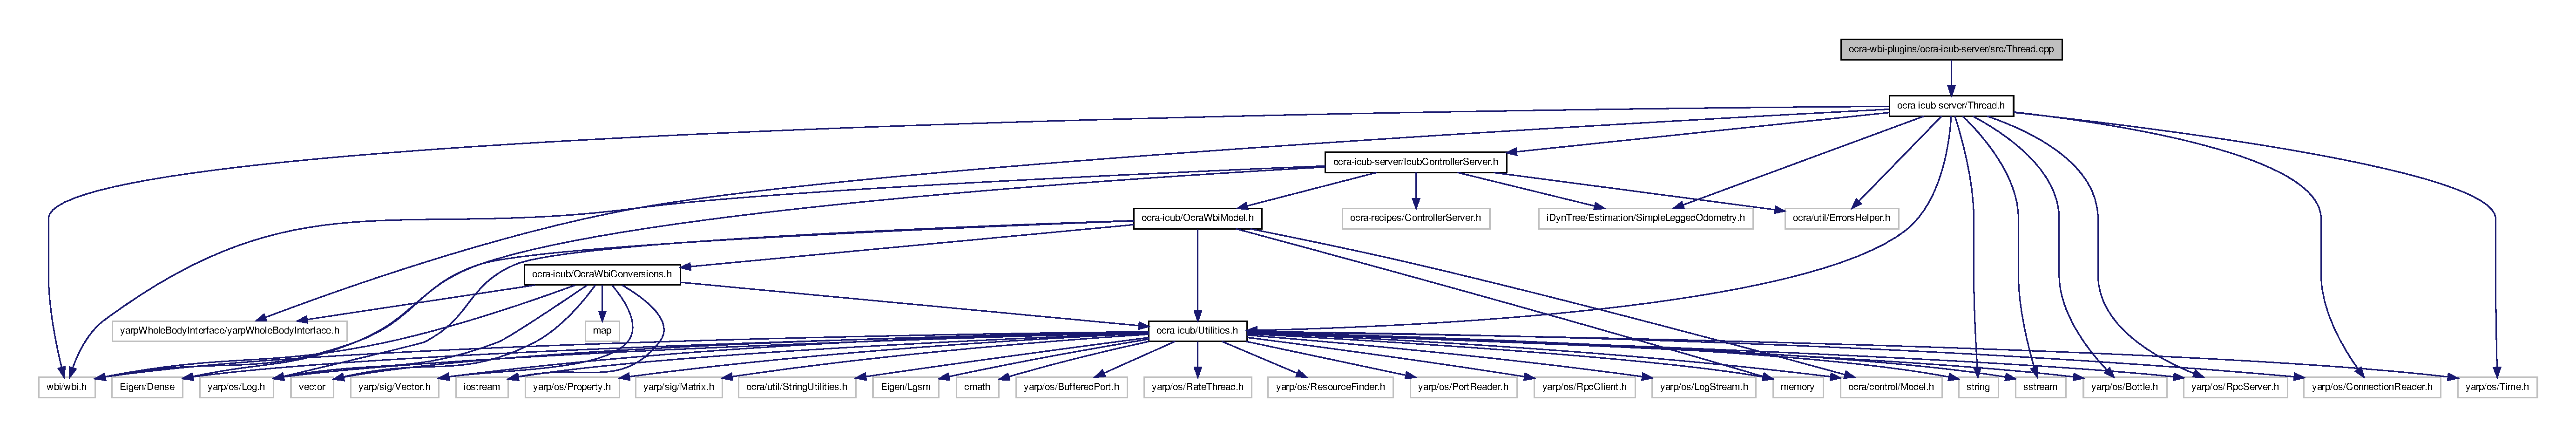
\includegraphics[width=350pt]{Thread_8cpp__incl}
\end{center}
\end{figure}
\subsection*{\-Functions}
\begin{DoxyCompactItemize}
\item 
std\-::ostream \& \hyperlink{Thread_8cpp_a30ab3a18ec4f8101aa6f1df6926888f6}{operator$<$$<$} (std\-::ostream \&out, const \hyperlink{classOcraControllerOptions}{\-Ocra\-Controller\-Options} \&opts)
\end{DoxyCompactItemize}


\subsection{\-Detailed \-Description}
\-The thread class for the controller server. \begin{DoxyAuthor}{\-Author}
\mbox{[}\-Ryan \-Lober\mbox{]}(\href{http://www.ryanlober.com}{\tt http\-://www.\-ryanlober.\-com}) 

\mbox{[}\-Antoine \-Hoarau\mbox{]}(\href{http://ahoarau.github.io}{\tt http\-://ahoarau.\-github.\-io}) 
\end{DoxyAuthor}
\begin{DoxyDate}{\-Date}
\-Feb 2016 
\end{DoxyDate}
\begin{DoxyCopyright}{\-Copyright}
\-G\-N\-U \-General \-Public \-License. 
\end{DoxyCopyright}


\subsection{\-Function \-Documentation}
\hypertarget{Thread_8cpp_a30ab3a18ec4f8101aa6f1df6926888f6}{\index{\-Thread.\-cpp@{\-Thread.\-cpp}!operator$<$$<$@{operator$<$$<$}}
\index{operator$<$$<$@{operator$<$$<$}!Thread.cpp@{\-Thread.\-cpp}}
\subsubsection[{operator$<$$<$}]{\setlength{\rightskip}{0pt plus 5cm}std\-::ostream\& operator$<$$<$ (
\begin{DoxyParamCaption}
\item[{std\-::ostream \&}]{out, }
\item[{const {\bf \-Ocra\-Controller\-Options} \&}]{opts}
\end{DoxyParamCaption}
)}}\label{Thread_8cpp_a30ab3a18ec4f8101aa6f1df6926888f6}

\hypertarget{IcubClient_8h}{\section{ocra-\/wbi-\/plugins/ocra-\/icub/include/ocra-\/icub/\-Icub\-Client.h \-File \-Reference}
\label{IcubClient_8h}\index{ocra-\/wbi-\/plugins/ocra-\/icub/include/ocra-\/icub/\-Icub\-Client.\-h@{ocra-\/wbi-\/plugins/ocra-\/icub/include/ocra-\/icub/\-Icub\-Client.\-h}}
}
{\ttfamily \#include $<$ocra-\/icub/\-Model\-Initializer.\-h$>$}\*
{\ttfamily \#include $<$ocra-\/icub/\-Ocra\-Wbi\-Conversions.\-h$>$}\*
{\ttfamily \#include $<$ocra-\/icub/\-Ocra\-Wbi\-Model.\-h$>$}\*
{\ttfamily \#include $<$ocra-\/icub/\-Utilities.\-h$>$}\*
\-Include dependency graph for \-Icub\-Client.\-h\-:\nopagebreak
\begin{figure}[H]
\begin{center}
\leavevmode
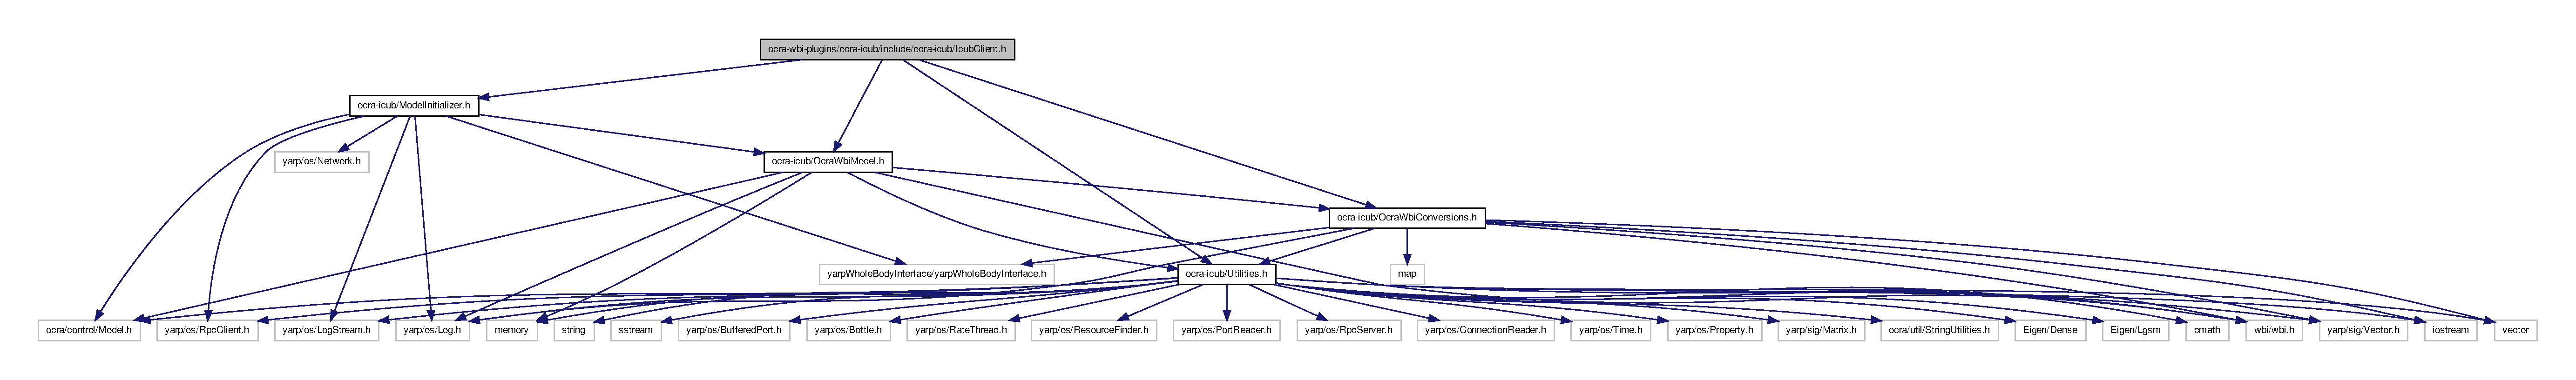
\includegraphics[width=350pt]{IcubClient_8h__incl}
\end{center}
\end{figure}
\-This graph shows which files directly or indirectly include this file\-:\nopagebreak
\begin{figure}[H]
\begin{center}
\leavevmode
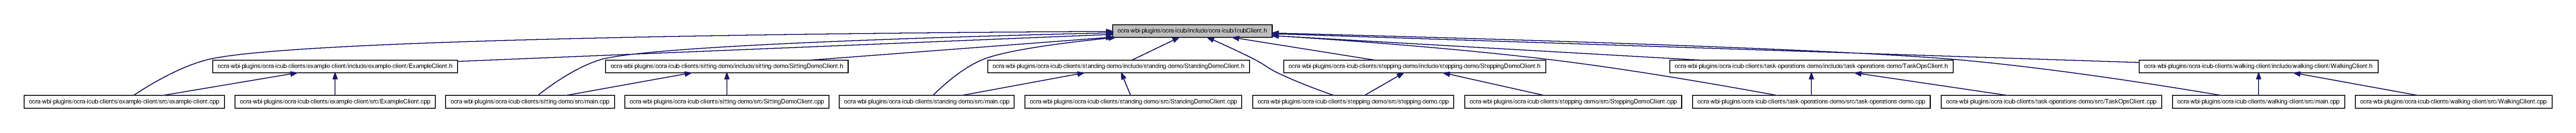
\includegraphics[width=350pt]{IcubClient_8h__dep__incl}
\end{center}
\end{figure}

\hypertarget{ModelInitializer_8h}{\section{ocra-\/wbi-\/plugins/ocra-\/icub/include/ocra-\/icub/\-Model\-Initializer.h \-File \-Reference}
\label{ModelInitializer_8h}\index{ocra-\/wbi-\/plugins/ocra-\/icub/include/ocra-\/icub/\-Model\-Initializer.\-h@{ocra-\/wbi-\/plugins/ocra-\/icub/include/ocra-\/icub/\-Model\-Initializer.\-h}}
}
{\ttfamily \#include $<$ocra-\/icub/\-Ocra\-Wbi\-Model.\-h$>$}\*
{\ttfamily \#include $<$ocra/control/\-Model.\-h$>$}\*
{\ttfamily \#include $<$yarp\-Whole\-Body\-Interface/yarp\-Whole\-Body\-Interface.\-h$>$}\*
{\ttfamily \#include $<$yarp/os/\-Rpc\-Client.\-h$>$}\*
{\ttfamily \#include $<$yarp/os/\-Network.\-h$>$}\*
{\ttfamily \#include $<$yarp/os/\-Log\-Stream.\-h$>$}\*
{\ttfamily \#include $<$yarp/os/\-Log.\-h$>$}\*
\-Include dependency graph for \-Model\-Initializer.\-h\-:\nopagebreak
\begin{figure}[H]
\begin{center}
\leavevmode
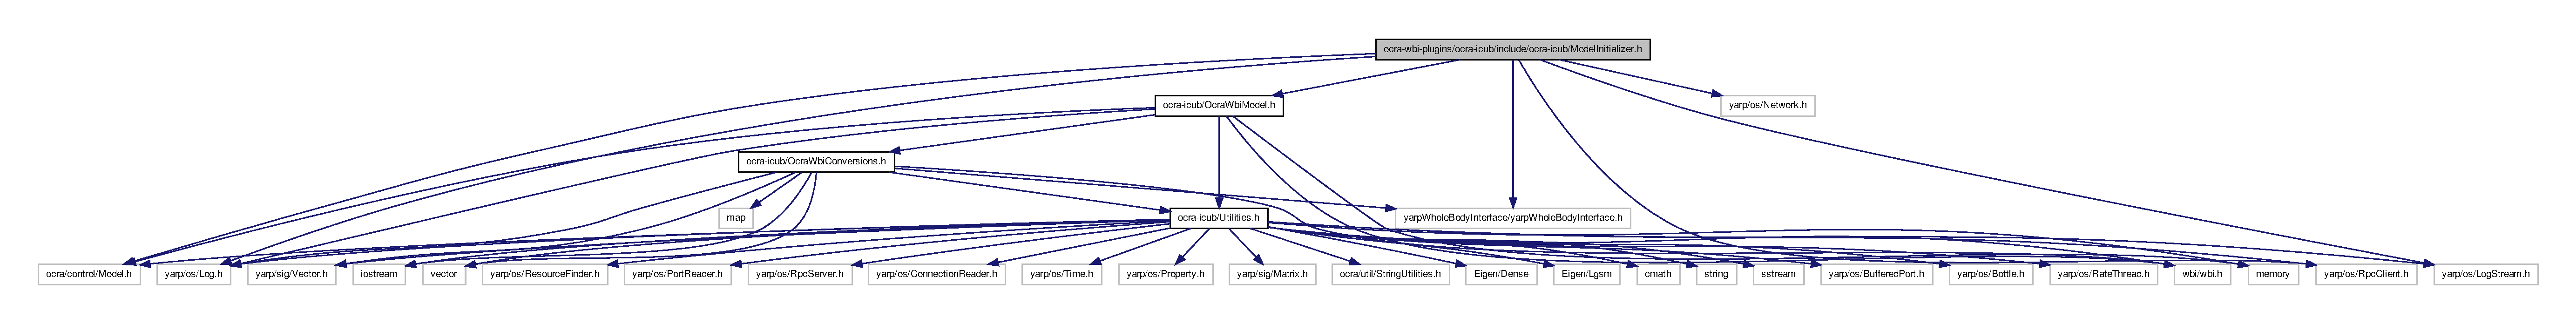
\includegraphics[width=350pt]{ModelInitializer_8h__incl}
\end{center}
\end{figure}
\-This graph shows which files directly or indirectly include this file\-:\nopagebreak
\begin{figure}[H]
\begin{center}
\leavevmode
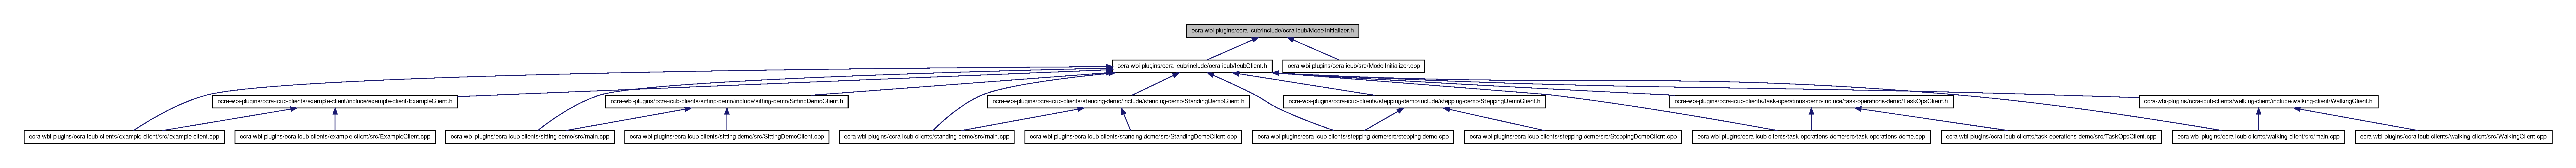
\includegraphics[width=350pt]{ModelInitializer_8h__dep__incl}
\end{center}
\end{figure}
\subsection*{\-Classes}
\begin{DoxyCompactItemize}
\item 
class \hyperlink{classocra__icub_1_1ModelInitializer}{ocra\-\_\-icub\-::\-Model\-Initializer}
\end{DoxyCompactItemize}
\subsection*{\-Namespaces}
\begin{DoxyCompactItemize}
\item 
namespace \hyperlink{namespaceocra__icub}{ocra\-\_\-icub}
\end{DoxyCompactItemize}

\hypertarget{OcraWbiConversions_8h}{\section{ocra-\/wbi-\/plugins/ocra-\/icub/include/ocra-\/icub/\-Ocra\-Wbi\-Conversions.h \-File \-Reference}
\label{OcraWbiConversions_8h}\index{ocra-\/wbi-\/plugins/ocra-\/icub/include/ocra-\/icub/\-Ocra\-Wbi\-Conversions.\-h@{ocra-\/wbi-\/plugins/ocra-\/icub/include/ocra-\/icub/\-Ocra\-Wbi\-Conversions.\-h}}
}


\-A utility class full of static conversion functions.  


{\ttfamily \#include $<$iostream$>$}\*
{\ttfamily \#include $<$map$>$}\*
{\ttfamily \#include $<$vector$>$}\*
{\ttfamily \#include $<$yarp/sig/\-Vector.\-h$>$}\*
{\ttfamily \#include $<$yarp/os/\-Log.\-h$>$}\*
{\ttfamily \#include $<$wbi/wbi.\-h$>$}\*
{\ttfamily \#include $<$yarp\-Whole\-Body\-Interface/yarp\-Whole\-Body\-Interface.\-h$>$}\*
{\ttfamily \#include \char`\"{}ocra-\/icub/\-Utilities.\-h\char`\"{}}\*
\-Include dependency graph for \-Ocra\-Wbi\-Conversions.\-h\-:\nopagebreak
\begin{figure}[H]
\begin{center}
\leavevmode
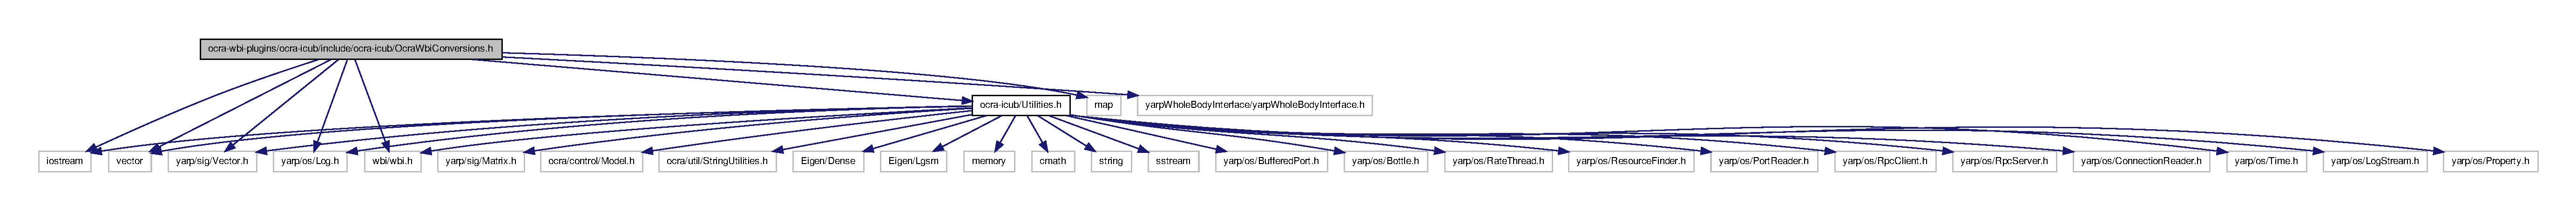
\includegraphics[width=350pt]{OcraWbiConversions_8h__incl}
\end{center}
\end{figure}
\-This graph shows which files directly or indirectly include this file\-:\nopagebreak
\begin{figure}[H]
\begin{center}
\leavevmode
\includegraphics[width=350pt]{OcraWbiConversions_8h__dep__incl}
\end{center}
\end{figure}
\subsection*{\-Classes}
\begin{DoxyCompactItemize}
\item 
class \hyperlink{classocra__icub_1_1OcraWbiConversions}{ocra\-\_\-icub\-::\-Ocra\-Wbi\-Conversions}
\end{DoxyCompactItemize}
\subsection*{\-Namespaces}
\begin{DoxyCompactItemize}
\item 
namespace \hyperlink{namespaceocra__icub}{ocra\-\_\-icub}
\end{DoxyCompactItemize}
\subsection*{\-Typedefs}
\begin{DoxyCompactItemize}
\item 
typedef \-Eigen\-::\-Matrix$<$ double, \*
\-Eigen\-::\-Dynamic, \-Eigen\-::\-Dynamic, \*
\-Eigen\-::\-Row\-Major $>$ \hyperlink{namespaceocra__icub_aa5e36a19ed031c28ca83c207bd7dd83f}{ocra\-\_\-icub\-::\-Matrix\-Xd\-Rm}
\end{DoxyCompactItemize}


\subsection{\-Detailed \-Description}
\-A utility class full of static conversion functions. \begin{DoxyAuthor}{\-Author}
\mbox{[}\-Ryan \-Lober\mbox{]}(\href{http://www.ryanlober.com}{\tt http\-://www.\-ryanlober.\-com}) 

\mbox{[}\-Antoine \-Hoarau\mbox{]}(\href{http://ahoarau.github.io}{\tt http\-://ahoarau.\-github.\-io}) 
\end{DoxyAuthor}
\begin{DoxyDate}{\-Date}
\-Feb 2016 
\end{DoxyDate}
\begin{DoxyCopyright}{\-Copyright}
\-G\-N\-U \-General \-Public \-License. 
\end{DoxyCopyright}

\hypertarget{OcraWbiModel_8h}{\section{ocra-\/wbi-\/plugins/ocra-\/icub/include/ocra-\/icub/\-Ocra\-Wbi\-Model.h \-File \-Reference}
\label{OcraWbiModel_8h}\index{ocra-\/wbi-\/plugins/ocra-\/icub/include/ocra-\/icub/\-Ocra\-Wbi\-Model.\-h@{ocra-\/wbi-\/plugins/ocra-\/icub/include/ocra-\/icub/\-Ocra\-Wbi\-Model.\-h}}
}


\-Implementation of ocra\-::\-Model using whole\-Body\-Interface.  


{\ttfamily \#include $<$memory$>$}\*
{\ttfamily \#include \char`\"{}ocra/control/\-Model.\-h\char`\"{}}\*
{\ttfamily \#include $<$wbi/wbi.\-h$>$}\*
{\ttfamily \#include $<$yarp/os/\-Log.\-h$>$}\*
{\ttfamily \#include \char`\"{}ocra-\/icub/\-Ocra\-Wbi\-Conversions.\-h\char`\"{}}\*
{\ttfamily \#include \char`\"{}ocra-\/icub/\-Utilities.\-h\char`\"{}}\*
\-Include dependency graph for \-Ocra\-Wbi\-Model.\-h\-:\nopagebreak
\begin{figure}[H]
\begin{center}
\leavevmode
\includegraphics[width=350pt]{OcraWbiModel_8h__incl}
\end{center}
\end{figure}
\-This graph shows which files directly or indirectly include this file\-:
\nopagebreak
\begin{figure}[H]
\begin{center}
\leavevmode
\includegraphics[width=350pt]{OcraWbiModel_8h__dep__incl}
\end{center}
\end{figure}
\subsection*{\-Classes}
\begin{DoxyCompactItemize}
\item 
class \hyperlink{classocra__icub_1_1OcraWbiModel}{ocra\-\_\-icub\-::\-Ocra\-Wbi\-Model}
\end{DoxyCompactItemize}
\subsection*{\-Namespaces}
\begin{DoxyCompactItemize}
\item 
namespace \hyperlink{namespaceocra__icub}{ocra\-\_\-icub}
\end{DoxyCompactItemize}


\subsection{\-Detailed \-Description}
\-Implementation of ocra\-::\-Model using whole\-Body\-Interface. \begin{DoxyAuthor}{\-Author}
\mbox{[}\-Ryan \-Lober\mbox{]}(\href{http://www.ryanlober.com}{\tt http\-://www.\-ryanlober.\-com}) 

\mbox{[}\-Antoine \-Hoarau\mbox{]}(\href{http://ahoarau.github.io}{\tt http\-://ahoarau.\-github.\-io}) 
\end{DoxyAuthor}
\begin{DoxyDate}{\-Date}
\-Feb 2016 
\end{DoxyDate}
\begin{DoxyCopyright}{\-Copyright}
\-G\-N\-U \-General \-Public \-License. 
\end{DoxyCopyright}

\hypertarget{Utilities_8h}{\section{ocra-\/wbi-\/plugins/ocra-\/icub/include/ocra-\/icub/\-Utilities.h \-File \-Reference}
\label{Utilities_8h}\index{ocra-\/wbi-\/plugins/ocra-\/icub/include/ocra-\/icub/\-Utilities.\-h@{ocra-\/wbi-\/plugins/ocra-\/icub/include/ocra-\/icub/\-Utilities.\-h}}
}


\-Some useful tools for the ocra-\/icub lib.  


{\ttfamily \#include $<$memory$>$}\*
{\ttfamily \#include $<$cmath$>$}\*
{\ttfamily \#include $<$iostream$>$}\*
{\ttfamily \#include $<$string$>$}\*
{\ttfamily \#include $<$vector$>$}\*
{\ttfamily \#include $<$sstream$>$}\*
{\ttfamily \#include $<$yarp/os/\-Buffered\-Port.\-h$>$}\*
{\ttfamily \#include $<$yarp/os/\-Bottle.\-h$>$}\*
{\ttfamily \#include $<$yarp/os/\-Rate\-Thread.\-h$>$}\*
{\ttfamily \#include $<$yarp/os/\-Resource\-Finder.\-h$>$}\*
{\ttfamily \#include $<$yarp/os/\-Port\-Reader.\-h$>$}\*
{\ttfamily \#include $<$yarp/os/\-Rpc\-Client.\-h$>$}\*
{\ttfamily \#include $<$yarp/os/\-Rpc\-Server.\-h$>$}\*
{\ttfamily \#include $<$yarp/os/\-Connection\-Reader.\-h$>$}\*
{\ttfamily \#include $<$yarp/os/\-Time.\-h$>$}\*
{\ttfamily \#include $<$yarp/os/\-Log.\-h$>$}\*
{\ttfamily \#include $<$yarp/os/\-Log\-Stream.\-h$>$}\*
{\ttfamily \#include $<$yarp/os/\-Property.\-h$>$}\*
{\ttfamily \#include $<$yarp/sig/\-Vector.\-h$>$}\*
{\ttfamily \#include $<$yarp/sig/\-Matrix.\-h$>$}\*
{\ttfamily \#include $<$wbi/wbi.\-h$>$}\*
{\ttfamily \#include \char`\"{}ocra/control/\-Model.\-h\char`\"{}}\*
{\ttfamily \#include \char`\"{}ocra/util/\-String\-Utilities.\-h\char`\"{}}\*
{\ttfamily \#include $<$\-Eigen/\-Dense$>$}\*
{\ttfamily \#include $<$\-Eigen/\-Lgsm$>$}\*
\-Include dependency graph for \-Utilities.\-h\-:
\nopagebreak
\begin{figure}[H]
\begin{center}
\leavevmode
\includegraphics[width=350pt]{Utilities_8h__incl}
\end{center}
\end{figure}
\-This graph shows which files directly or indirectly include this file\-:
\nopagebreak
\begin{figure}[H]
\begin{center}
\leavevmode
\includegraphics[width=350pt]{Utilities_8h__dep__incl}
\end{center}
\end{figure}
\subsection*{\-Namespaces}
\begin{DoxyCompactItemize}
\item 
namespace \hyperlink{namespaceocra__icub}{ocra\-\_\-icub}
\end{DoxyCompactItemize}
\subsection*{\-Defines}
\begin{DoxyCompactItemize}
\item 
\#define \hyperlink{Utilities_8h_a986e6d54948ebf3007dc52bd0fc737be}{\-C\-L\-A\-S\-S\-\_\-\-P\-O\-I\-N\-T\-E\-R\-\_\-\-T\-Y\-P\-E\-D\-E\-F\-S}(\-Class)
\end{DoxyCompactItemize}
\subsection*{\-Enumerations}
\begin{DoxyCompactItemize}
\item 
enum \hyperlink{namespaceocra__icub_afbd2db66b68005fb7cfac19210caf83f}{ocra\-\_\-icub\-::\-O\-C\-R\-A\-\_\-\-I\-C\-U\-B\-\_\-\-M\-E\-S\-S\-A\-G\-E} \{ \*
\hyperlink{namespaceocra__icub_afbd2db66b68005fb7cfac19210caf83fafa982af27b4e13f109d8769472d75217}{ocra\-\_\-icub\-::\-S\-T\-R\-I\-N\-G\-\_\-\-M\-E\-S\-S\-A\-G\-E} =  -\/1, 
\hyperlink{namespaceocra__icub_afbd2db66b68005fb7cfac19210caf83faa0c1832978fad84ef108d48265af68d2}{ocra\-\_\-icub\-::\-F\-A\-I\-L\-U\-R\-E} =  0, 
\hyperlink{namespaceocra__icub_afbd2db66b68005fb7cfac19210caf83fa67c96e3afcb39533f69c97dc5e9734e5}{ocra\-\_\-icub\-::\-S\-U\-C\-C\-E\-S\-S}, 
\hyperlink{namespaceocra__icub_afbd2db66b68005fb7cfac19210caf83fae8fe02f5f3b1b11d4749e720b9ec3636}{ocra\-\_\-icub\-::\-G\-E\-T\-\_\-\-M\-O\-D\-E\-L\-\_\-\-C\-O\-N\-F\-I\-G\-\_\-\-I\-N\-F\-O}, 
\*
\hyperlink{namespaceocra__icub_afbd2db66b68005fb7cfac19210caf83fa772ab917d1ff28db029af9271208a69a}{ocra\-\_\-icub\-::\-G\-E\-T\-\_\-\-C\-O\-N\-T\-R\-O\-L\-L\-E\-R\-\_\-\-S\-E\-R\-V\-E\-R\-\_\-\-S\-T\-A\-T\-U\-S}, 
\hyperlink{namespaceocra__icub_afbd2db66b68005fb7cfac19210caf83fa5dee3cfa0ab6c29f5546bc9e30c0aef5}{ocra\-\_\-icub\-::\-C\-O\-N\-T\-R\-O\-L\-L\-E\-R\-\_\-\-S\-E\-R\-V\-E\-R\-\_\-\-R\-U\-N\-N\-I\-N\-G}, 
\hyperlink{namespaceocra__icub_afbd2db66b68005fb7cfac19210caf83fafd31e40d18e553fc09105d360455bc49}{ocra\-\_\-icub\-::\-C\-O\-N\-T\-R\-O\-L\-L\-E\-R\-\_\-\-S\-E\-R\-V\-E\-R\-\_\-\-S\-T\-O\-P\-P\-E\-D}, 
\hyperlink{namespaceocra__icub_afbd2db66b68005fb7cfac19210caf83fa48ad7962d035a58257a0381872ce27b1}{ocra\-\_\-icub\-::\-C\-O\-N\-T\-R\-O\-L\-L\-E\-R\-\_\-\-S\-E\-R\-V\-E\-R\-\_\-\-P\-A\-U\-S\-E\-D}, 
\*
\hyperlink{namespaceocra__icub_afbd2db66b68005fb7cfac19210caf83fafd78d107914396f475c3b12d2b31ea2a}{ocra\-\_\-icub\-::\-G\-E\-T\-\_\-\-L\-\_\-\-F\-O\-O\-T\-\_\-\-P\-O\-S\-E}, 
\hyperlink{namespaceocra__icub_afbd2db66b68005fb7cfac19210caf83fae7c9fa2563b6c0b14e5b05d1794dac36}{ocra\-\_\-icub\-::\-H\-E\-L\-P}
 \}
\end{DoxyCompactItemize}
\subsection*{\-Functions}
\begin{DoxyCompactItemize}
\item 
void \hyperlink{namespaceocra__icub_a07ffe33877389b6b111944e8a666e221}{ocra\-\_\-icub\-::get\-Nominal\-Posture} (const ocra\-::\-Model \&model, \-Eigen\-::\-Vector\-Xd \&q)
\item 
void \hyperlink{namespaceocra__icub_a91c3caf94014ea9988e56dd2572768ce}{ocra\-\_\-icub\-::get\-Home\-Posture} (const ocra\-::\-Model \&model, \-Eigen\-::\-Vector\-Xd \&q)
\end{DoxyCompactItemize}
\subsection*{\-Variables}
\begin{DoxyCompactItemize}
\item 
static constexpr double \hyperlink{namespaceocra__icub_ab06477ded34ed5514b911a3511b22e3d}{ocra\-\_\-icub\-::\-D\-E\-G\-\_\-\-T\-O\-\_\-\-R\-A\-D} = \-M\-\_\-\-P\-I/180.\-0
\end{DoxyCompactItemize}


\subsection{\-Detailed \-Description}
\-Some useful tools for the ocra-\/icub lib. \-This file is for all the various macros and helper classes that are generic to ocra-\/icub. \-It is also a place for all the repeated includes like standard stl includes etc. \begin{DoxyAuthor}{\-Author}
\mbox{[}\-Ryan \-Lober\mbox{]}(\href{http://www.ryanlober.com}{\tt http\-://www.\-ryanlober.\-com}) 
\end{DoxyAuthor}
\begin{DoxyDate}{\-Date}
\-Feb 2016 
\end{DoxyDate}
\begin{DoxyCopyright}{\-Copyright}
\-G\-N\-U \-General \-Public \-License. 
\end{DoxyCopyright}


\subsection{\-Define \-Documentation}
\hypertarget{Utilities_8h_a986e6d54948ebf3007dc52bd0fc737be}{\index{\-Utilities.\-h@{\-Utilities.\-h}!\-C\-L\-A\-S\-S\-\_\-\-P\-O\-I\-N\-T\-E\-R\-\_\-\-T\-Y\-P\-E\-D\-E\-F\-S@{\-C\-L\-A\-S\-S\-\_\-\-P\-O\-I\-N\-T\-E\-R\-\_\-\-T\-Y\-P\-E\-D\-E\-F\-S}}
\index{\-C\-L\-A\-S\-S\-\_\-\-P\-O\-I\-N\-T\-E\-R\-\_\-\-T\-Y\-P\-E\-D\-E\-F\-S@{\-C\-L\-A\-S\-S\-\_\-\-P\-O\-I\-N\-T\-E\-R\-\_\-\-T\-Y\-P\-E\-D\-E\-F\-S}!Utilities.h@{\-Utilities.\-h}}
\subsubsection[{\-C\-L\-A\-S\-S\-\_\-\-P\-O\-I\-N\-T\-E\-R\-\_\-\-T\-Y\-P\-E\-D\-E\-F\-S}]{\setlength{\rightskip}{0pt plus 5cm}\#define {\bf \-C\-L\-A\-S\-S\-\_\-\-P\-O\-I\-N\-T\-E\-R\-\_\-\-T\-Y\-P\-E\-D\-E\-F\-S}(
\begin{DoxyParamCaption}
\item[{}]{\-Class}
\end{DoxyParamCaption}
)}}\label{Utilities_8h_a986e6d54948ebf3007dc52bd0fc737be}
{\bfseries \-Value\-:}
\begin{DoxyCode}
public:\
using ptr           = std::shared_ptr   <Class>;  \
using shared_ptr    = std::shared_ptr   <Class>;  \
using unique_ptr    = std::unique_ptr   <Class>;  \
using weak_ptr      = std::weak_ptr     <Class>;  \
using const_ptr           = const std::shared_ptr   <Class>;  \
using const_shared_ptr    = const std::shared_ptr   <Class>;  \
using const_unique_ptr    = const std::unique_ptr   <Class>;  \
using const_weak_ptr      = const std::weak_ptr     <Class>;
\end{DoxyCode}
\-Macro function which basically just defines pointer typdefs for classes. \-Note that normally macros are evil monsters but \-I think this is a perfect usage case to cut down on repeated code. 
\begin{DoxyParams}{\-Parameters}
{\em \-Class} & \-Just pop this bad boy below the class definition and it will do the rest. \\
\hline
\end{DoxyParams}

\hypertarget{ModelInitializer_8cpp}{\section{ocra-\/wbi-\/plugins/ocra-\/icub/src/\-Model\-Initializer.cpp \-File \-Reference}
\label{ModelInitializer_8cpp}\index{ocra-\/wbi-\/plugins/ocra-\/icub/src/\-Model\-Initializer.\-cpp@{ocra-\/wbi-\/plugins/ocra-\/icub/src/\-Model\-Initializer.\-cpp}}
}
{\ttfamily \#include $<$ocra-\/icub/\-Model\-Initializer.\-h$>$}\*
\-Include dependency graph for \-Model\-Initializer.\-cpp\-:
\nopagebreak
\begin{figure}[H]
\begin{center}
\leavevmode
\includegraphics[width=350pt]{ModelInitializer_8cpp__incl}
\end{center}
\end{figure}

\hypertarget{OcraWbiConversions_8cpp}{\section{ocra-\/wbi-\/plugins/ocra-\/icub/src/\-Ocra\-Wbi\-Conversions.cpp \-File \-Reference}
\label{OcraWbiConversions_8cpp}\index{ocra-\/wbi-\/plugins/ocra-\/icub/src/\-Ocra\-Wbi\-Conversions.\-cpp@{ocra-\/wbi-\/plugins/ocra-\/icub/src/\-Ocra\-Wbi\-Conversions.\-cpp}}
}


\-A utility class full of static conversion functions.  


{\ttfamily \#include $<$ocra-\/icub/\-Ocra\-Wbi\-Conversions.\-h$>$}\*
\-Include dependency graph for \-Ocra\-Wbi\-Conversions.\-cpp\-:\nopagebreak
\begin{figure}[H]
\begin{center}
\leavevmode
\includegraphics[width=350pt]{OcraWbiConversions_8cpp__incl}
\end{center}
\end{figure}


\subsection{\-Detailed \-Description}
\-A utility class full of static conversion functions. \begin{DoxyAuthor}{\-Author}
\mbox{[}\-Ryan \-Lober\mbox{]}(\href{http://www.ryanlober.com}{\tt http\-://www.\-ryanlober.\-com}) 

\mbox{[}\-Antoine \-Hoarau\mbox{]}(\href{http://ahoarau.github.io}{\tt http\-://ahoarau.\-github.\-io}) 
\end{DoxyAuthor}
\begin{DoxyDate}{\-Date}
\-Feb 2016 
\end{DoxyDate}
\begin{DoxyCopyright}{\-Copyright}
\-G\-N\-U \-General \-Public \-License. 
\end{DoxyCopyright}

\hypertarget{OcraWbiModel_8cpp}{\section{ocra-\/wbi-\/plugins/ocra-\/icub/src/\-Ocra\-Wbi\-Model.cpp \-File \-Reference}
\label{OcraWbiModel_8cpp}\index{ocra-\/wbi-\/plugins/ocra-\/icub/src/\-Ocra\-Wbi\-Model.\-cpp@{ocra-\/wbi-\/plugins/ocra-\/icub/src/\-Ocra\-Wbi\-Model.\-cpp}}
}


\-Implementation of ocra\-::\-Model using whole\-Body\-Interface.  


{\ttfamily \#include $<$ocra-\/icub/\-Ocra\-Wbi\-Model.\-h$>$}\*
\-Include dependency graph for \-Ocra\-Wbi\-Model.\-cpp\-:\nopagebreak
\begin{figure}[H]
\begin{center}
\leavevmode
\includegraphics[width=350pt]{OcraWbiModel_8cpp__incl}
\end{center}
\end{figure}
\subsection*{\-Classes}
\begin{DoxyCompactItemize}
\item 
struct \hyperlink{structOcraWbiModel_1_1OcraWbiModel__pimpl}{ocra\-\_\-icub\-::\-Ocra\-Wbi\-Model\-::\-Ocra\-Wbi\-Model\-\_\-pimpl}
\end{DoxyCompactItemize}
\subsection*{\-Defines}
\begin{DoxyCompactItemize}
\item 
\#define \hyperlink{OcraWbiModel_8cpp_a7f4e728fa0fd89911a2c60c42c0d4560}{\-A\-L\-L\-\_\-\-J\-O\-I\-N\-T\-S}~-\/1
\item 
\#define \hyperlink{OcraWbiModel_8cpp_a29de1200631802e23f75bbd14adcc082}{\-F\-R\-E\-E\-\_\-\-R\-O\-O\-T\-\_\-\-D\-O\-F}~6
\item 
\#define \hyperlink{OcraWbiModel_8cpp_a72cb22de2538ae949cc73fa3d7c33bdc}{\-C\-O\-M\-\_\-\-P\-O\-S\-\_\-\-D\-I\-M}~3
\item 
\#define \hyperlink{OcraWbiModel_8cpp_ab4a87cb824ceff256c6b8bce7701af58}{\-T\-R\-A\-N\-S\-\_\-\-R\-O\-T\-\_\-\-D\-I\-M}~6
\item 
\#define \hyperlink{OcraWbiModel_8cpp_afbb98f526272c46369f405eee4e9d9aa}{\-G\-R\-A\-V\-I\-T\-Y\-\_\-\-C\-O\-N\-S\-T\-A\-N\-T}~-\/9.\-81
\end{DoxyCompactItemize}
\subsection*{\-Typedefs}
\begin{DoxyCompactItemize}
\item 
typedef \*
\hyperlink{OcraWbiModel_8cpp_a2ee3f7feea423a8bc6b8fbcea1d4e217}{\-Eigen\-::\-Displacementd\-::\-Adjoint\-Matrix} \hyperlink{OcraWbiModel_8cpp_a2ee3f7feea423a8bc6b8fbcea1d4e217}{\-Adjoint\-Matrix}
\end{DoxyCompactItemize}
\subsection*{\-Variables}
\begin{DoxyCompactItemize}
\item 
const double \hyperlink{OcraWbiModel_8cpp_a3cdc4ec85b339c11e5b34ce069bf7077}{g\-\_\-vector} \mbox{[}3\mbox{]} = \{0, 0, \hyperlink{OcraWbiModel_8cpp_afbb98f526272c46369f405eee4e9d9aa}{\-G\-R\-A\-V\-I\-T\-Y\-\_\-\-C\-O\-N\-S\-T\-A\-N\-T}\}
\end{DoxyCompactItemize}


\subsection{\-Detailed \-Description}
\-Implementation of ocra\-::\-Model using whole\-Body\-Interface. \begin{DoxyAuthor}{\-Author}
\mbox{[}\-Ryan \-Lober\mbox{]}(\href{http://www.ryanlober.com}{\tt http\-://www.\-ryanlober.\-com}) 

\mbox{[}\-Antoine \-Hoarau\mbox{]}(\href{http://ahoarau.github.io}{\tt http\-://ahoarau.\-github.\-io}) 
\end{DoxyAuthor}
\begin{DoxyDate}{\-Date}
\-Feb 2016 
\end{DoxyDate}
\begin{DoxyCopyright}{\-Copyright}
\-G\-N\-U \-General \-Public \-License. 
\end{DoxyCopyright}


\subsection{\-Define \-Documentation}
\hypertarget{OcraWbiModel_8cpp_a7f4e728fa0fd89911a2c60c42c0d4560}{\index{\-Ocra\-Wbi\-Model.\-cpp@{\-Ocra\-Wbi\-Model.\-cpp}!\-A\-L\-L\-\_\-\-J\-O\-I\-N\-T\-S@{\-A\-L\-L\-\_\-\-J\-O\-I\-N\-T\-S}}
\index{\-A\-L\-L\-\_\-\-J\-O\-I\-N\-T\-S@{\-A\-L\-L\-\_\-\-J\-O\-I\-N\-T\-S}!OcraWbiModel.cpp@{\-Ocra\-Wbi\-Model.\-cpp}}
\subsubsection[{\-A\-L\-L\-\_\-\-J\-O\-I\-N\-T\-S}]{\setlength{\rightskip}{0pt plus 5cm}\#define {\bf \-A\-L\-L\-\_\-\-J\-O\-I\-N\-T\-S}~-\/1}}\label{OcraWbiModel_8cpp_a7f4e728fa0fd89911a2c60c42c0d4560}
\hypertarget{OcraWbiModel_8cpp_a72cb22de2538ae949cc73fa3d7c33bdc}{\index{\-Ocra\-Wbi\-Model.\-cpp@{\-Ocra\-Wbi\-Model.\-cpp}!\-C\-O\-M\-\_\-\-P\-O\-S\-\_\-\-D\-I\-M@{\-C\-O\-M\-\_\-\-P\-O\-S\-\_\-\-D\-I\-M}}
\index{\-C\-O\-M\-\_\-\-P\-O\-S\-\_\-\-D\-I\-M@{\-C\-O\-M\-\_\-\-P\-O\-S\-\_\-\-D\-I\-M}!OcraWbiModel.cpp@{\-Ocra\-Wbi\-Model.\-cpp}}
\subsubsection[{\-C\-O\-M\-\_\-\-P\-O\-S\-\_\-\-D\-I\-M}]{\setlength{\rightskip}{0pt plus 5cm}\#define {\bf \-C\-O\-M\-\_\-\-P\-O\-S\-\_\-\-D\-I\-M}~3}}\label{OcraWbiModel_8cpp_a72cb22de2538ae949cc73fa3d7c33bdc}
\hypertarget{OcraWbiModel_8cpp_a29de1200631802e23f75bbd14adcc082}{\index{\-Ocra\-Wbi\-Model.\-cpp@{\-Ocra\-Wbi\-Model.\-cpp}!\-F\-R\-E\-E\-\_\-\-R\-O\-O\-T\-\_\-\-D\-O\-F@{\-F\-R\-E\-E\-\_\-\-R\-O\-O\-T\-\_\-\-D\-O\-F}}
\index{\-F\-R\-E\-E\-\_\-\-R\-O\-O\-T\-\_\-\-D\-O\-F@{\-F\-R\-E\-E\-\_\-\-R\-O\-O\-T\-\_\-\-D\-O\-F}!OcraWbiModel.cpp@{\-Ocra\-Wbi\-Model.\-cpp}}
\subsubsection[{\-F\-R\-E\-E\-\_\-\-R\-O\-O\-T\-\_\-\-D\-O\-F}]{\setlength{\rightskip}{0pt plus 5cm}\#define {\bf \-F\-R\-E\-E\-\_\-\-R\-O\-O\-T\-\_\-\-D\-O\-F}~6}}\label{OcraWbiModel_8cpp_a29de1200631802e23f75bbd14adcc082}
\hypertarget{OcraWbiModel_8cpp_afbb98f526272c46369f405eee4e9d9aa}{\index{\-Ocra\-Wbi\-Model.\-cpp@{\-Ocra\-Wbi\-Model.\-cpp}!\-G\-R\-A\-V\-I\-T\-Y\-\_\-\-C\-O\-N\-S\-T\-A\-N\-T@{\-G\-R\-A\-V\-I\-T\-Y\-\_\-\-C\-O\-N\-S\-T\-A\-N\-T}}
\index{\-G\-R\-A\-V\-I\-T\-Y\-\_\-\-C\-O\-N\-S\-T\-A\-N\-T@{\-G\-R\-A\-V\-I\-T\-Y\-\_\-\-C\-O\-N\-S\-T\-A\-N\-T}!OcraWbiModel.cpp@{\-Ocra\-Wbi\-Model.\-cpp}}
\subsubsection[{\-G\-R\-A\-V\-I\-T\-Y\-\_\-\-C\-O\-N\-S\-T\-A\-N\-T}]{\setlength{\rightskip}{0pt plus 5cm}\#define {\bf \-G\-R\-A\-V\-I\-T\-Y\-\_\-\-C\-O\-N\-S\-T\-A\-N\-T}~-\/9.\-81}}\label{OcraWbiModel_8cpp_afbb98f526272c46369f405eee4e9d9aa}
\hypertarget{OcraWbiModel_8cpp_ab4a87cb824ceff256c6b8bce7701af58}{\index{\-Ocra\-Wbi\-Model.\-cpp@{\-Ocra\-Wbi\-Model.\-cpp}!\-T\-R\-A\-N\-S\-\_\-\-R\-O\-T\-\_\-\-D\-I\-M@{\-T\-R\-A\-N\-S\-\_\-\-R\-O\-T\-\_\-\-D\-I\-M}}
\index{\-T\-R\-A\-N\-S\-\_\-\-R\-O\-T\-\_\-\-D\-I\-M@{\-T\-R\-A\-N\-S\-\_\-\-R\-O\-T\-\_\-\-D\-I\-M}!OcraWbiModel.cpp@{\-Ocra\-Wbi\-Model.\-cpp}}
\subsubsection[{\-T\-R\-A\-N\-S\-\_\-\-R\-O\-T\-\_\-\-D\-I\-M}]{\setlength{\rightskip}{0pt plus 5cm}\#define {\bf \-T\-R\-A\-N\-S\-\_\-\-R\-O\-T\-\_\-\-D\-I\-M}~6}}\label{OcraWbiModel_8cpp_ab4a87cb824ceff256c6b8bce7701af58}


\subsection{\-Typedef \-Documentation}
\hypertarget{OcraWbiModel_8cpp_a2ee3f7feea423a8bc6b8fbcea1d4e217}{\index{\-Ocra\-Wbi\-Model.\-cpp@{\-Ocra\-Wbi\-Model.\-cpp}!\-Adjoint\-Matrix@{\-Adjoint\-Matrix}}
\index{\-Adjoint\-Matrix@{\-Adjoint\-Matrix}!OcraWbiModel.cpp@{\-Ocra\-Wbi\-Model.\-cpp}}
\subsubsection[{\-Adjoint\-Matrix}]{\setlength{\rightskip}{0pt plus 5cm}typedef {\bf \-Eigen\-::\-Displacementd\-::\-Adjoint\-Matrix} {\bf \-Adjoint\-Matrix}}}\label{OcraWbiModel_8cpp_a2ee3f7feea423a8bc6b8fbcea1d4e217}


\subsection{\-Variable \-Documentation}
\hypertarget{OcraWbiModel_8cpp_a3cdc4ec85b339c11e5b34ce069bf7077}{\index{\-Ocra\-Wbi\-Model.\-cpp@{\-Ocra\-Wbi\-Model.\-cpp}!g\-\_\-vector@{g\-\_\-vector}}
\index{g\-\_\-vector@{g\-\_\-vector}!OcraWbiModel.cpp@{\-Ocra\-Wbi\-Model.\-cpp}}
\subsubsection[{g\-\_\-vector}]{\setlength{\rightskip}{0pt plus 5cm}const double {\bf g\-\_\-vector}\mbox{[}3\mbox{]} = \{0, 0, {\bf \-G\-R\-A\-V\-I\-T\-Y\-\_\-\-C\-O\-N\-S\-T\-A\-N\-T}\}}}\label{OcraWbiModel_8cpp_a3cdc4ec85b339c11e5b34ce069bf7077}

\hypertarget{Utilities_8cpp}{\section{ocra-\/wbi-\/plugins/ocra-\/icub/src/\-Utilities.cpp \-File \-Reference}
\label{Utilities_8cpp}\index{ocra-\/wbi-\/plugins/ocra-\/icub/src/\-Utilities.\-cpp@{ocra-\/wbi-\/plugins/ocra-\/icub/src/\-Utilities.\-cpp}}
}


\-Some useful tools for the ocra-\/icub lib.  


{\ttfamily \#include \char`\"{}ocra-\/icub/\-Utilities.\-h\char`\"{}}\*
\-Include dependency graph for \-Utilities.\-cpp\-:
\nopagebreak
\begin{figure}[H]
\begin{center}
\leavevmode
\includegraphics[width=350pt]{Utilities_8cpp__incl}
\end{center}
\end{figure}
\subsection*{\-Functions}
\begin{DoxyCompactItemize}
\item 
void \hyperlink{Utilities_8cpp_a666768e3a20bb81b9df67e3814a783bb}{get\-Nominal\-Posture} (const ocra\-::\-Model \&model, \-Eigen\-::\-Vector\-Xd \&q)
\item 
void \hyperlink{Utilities_8cpp_aeeff320b9cc14a9a7cf72fcfbdada2f6}{get\-Home\-Posture} (const ocra\-::\-Model \&model, \-Eigen\-::\-Vector\-Xd \&q)
\end{DoxyCompactItemize}


\subsection{\-Detailed \-Description}
\-Some useful tools for the ocra-\/icub lib. \-This file is for all the various macros and helper classes that are generic to ocra-\/icub. \-It is also a place for all the repeated includes like standard stl includes etc. \begin{DoxyAuthor}{\-Author}
\mbox{[}\-Ryan \-Lober\mbox{]}(\href{http://www.ryanlober.com}{\tt http\-://www.\-ryanlober.\-com}) 
\end{DoxyAuthor}
\begin{DoxyDate}{\-Date}
\-Feb 2016 
\end{DoxyDate}
\begin{DoxyCopyright}{\-Copyright}
\-G\-N\-U \-General \-Public \-License. 
\end{DoxyCopyright}


\subsection{\-Function \-Documentation}
\hypertarget{Utilities_8cpp_aeeff320b9cc14a9a7cf72fcfbdada2f6}{\index{\-Utilities.\-cpp@{\-Utilities.\-cpp}!get\-Home\-Posture@{get\-Home\-Posture}}
\index{get\-Home\-Posture@{get\-Home\-Posture}!Utilities.cpp@{\-Utilities.\-cpp}}
\subsubsection[{get\-Home\-Posture}]{\setlength{\rightskip}{0pt plus 5cm}void {\bf get\-Home\-Posture} (
\begin{DoxyParamCaption}
\item[{const ocra\-::\-Model \&}]{model, }
\item[{\-Eigen\-::\-Vector\-Xd \&}]{q}
\end{DoxyParamCaption}
)}}\label{Utilities_8cpp_aeeff320b9cc14a9a7cf72fcfbdada2f6}
\hypertarget{Utilities_8cpp_a666768e3a20bb81b9df67e3814a783bb}{\index{\-Utilities.\-cpp@{\-Utilities.\-cpp}!get\-Nominal\-Posture@{get\-Nominal\-Posture}}
\index{get\-Nominal\-Posture@{get\-Nominal\-Posture}!Utilities.cpp@{\-Utilities.\-cpp}}
\subsubsection[{get\-Nominal\-Posture}]{\setlength{\rightskip}{0pt plus 5cm}void {\bf get\-Nominal\-Posture} (
\begin{DoxyParamCaption}
\item[{const ocra\-::\-Model \&}]{model, }
\item[{\-Eigen\-::\-Vector\-Xd \&}]{q}
\end{DoxyParamCaption}
)}}\label{Utilities_8cpp_a666768e3a20bb81b9df67e3814a783bb}

\hypertarget{README_8md}{\section{ocra-\/wbi-\/plugins/\-R\-E\-A\-D\-M\-E.md \-File \-Reference}
\label{README_8md}\index{ocra-\/wbi-\/plugins/\-R\-E\-A\-D\-M\-E.\-md@{ocra-\/wbi-\/plugins/\-R\-E\-A\-D\-M\-E.\-md}}
}
\subsection*{\-Functions}
\begin{DoxyCompactItemize}
\item 
\-Controller implementations and \*
plugins for communicating \*
between the whole body \*
controller libraries developed \*
at calls the \hyperlink{README_8md_ae8b57eb96384b7265d50bd361b6e1a3e}{compute\-Torque} ()`function and then sends it to the robot.\-The rest of the code is designed around yarp`\-R\-F\-Module`and`\-Rate\-Thread`
\end{DoxyCompactItemize}
\subsection*{\-Variables}
\begin{DoxyCompactItemize}
\item 
\-Controller implementations and \*
plugins for communicating \*
between the whole body \*
controller libraries developed \*
at \hyperlink{README_8md_a5b08a8c96b07654a96b4a53b36d91f57}{\-I\-S\-I\-R}
\item 
\-Controller implementations and \*
plugins for communicating \*
between the whole body \*
controller libraries developed \*
at \hyperlink{README_8md_a504ae18f7038ea6e495dcd4d13a5039d}{https}
\item 
\-Controller implementations and \*
plugins for communicating \*
between the whole body \*
controller libraries developed \*
at calls the to parse command \*
line \hyperlink{README_8md_ae7fe72c1608a83b1bac9259edeb8d53d}{args}
\end{DoxyCompactItemize}


\subsection{\-Function \-Documentation}
\hypertarget{README_8md_ae8b57eb96384b7265d50bd361b6e1a3e}{\index{\-R\-E\-A\-D\-M\-E.\-md@{\-R\-E\-A\-D\-M\-E.\-md}!compute\-Torque@{compute\-Torque}}
\index{compute\-Torque@{compute\-Torque}!README.md@{\-R\-E\-A\-D\-M\-E.\-md}}
\subsubsection[{compute\-Torque}]{\setlength{\rightskip}{0pt plus 5cm}\-Controller implementations and plugins for communicating between the whole body controller libraries developed at calls the {\bf compute\-Torque} (
\begin{DoxyParamCaption}
{}
\end{DoxyParamCaption}
)}}\label{README_8md_ae8b57eb96384b7265d50bd361b6e1a3e}


\subsection{\-Variable \-Documentation}
\hypertarget{README_8md_ae7fe72c1608a83b1bac9259edeb8d53d}{\index{\-R\-E\-A\-D\-M\-E.\-md@{\-R\-E\-A\-D\-M\-E.\-md}!args@{args}}
\index{args@{args}!README.md@{\-R\-E\-A\-D\-M\-E.\-md}}
\subsubsection[{args}]{\setlength{\rightskip}{0pt plus 5cm}\-Controller implementations and plugins for communicating between the whole body controller libraries developed at calls the to parse command line {\bf args}}}\label{README_8md_ae7fe72c1608a83b1bac9259edeb8d53d}
\hypertarget{README_8md_a504ae18f7038ea6e495dcd4d13a5039d}{\index{\-R\-E\-A\-D\-M\-E.\-md@{\-R\-E\-A\-D\-M\-E.\-md}!https@{https}}
\index{https@{https}!README.md@{\-R\-E\-A\-D\-M\-E.\-md}}
\subsubsection[{https}]{\setlength{\rightskip}{0pt plus 5cm}\-Controller implementations and plugins for communicating between the whole body controller libraries developed at {\bf https}}}\label{README_8md_a504ae18f7038ea6e495dcd4d13a5039d}
\hypertarget{README_8md_a5b08a8c96b07654a96b4a53b36d91f57}{\index{\-R\-E\-A\-D\-M\-E.\-md@{\-R\-E\-A\-D\-M\-E.\-md}!\-I\-S\-I\-R@{\-I\-S\-I\-R}}
\index{\-I\-S\-I\-R@{\-I\-S\-I\-R}!README.md@{\-R\-E\-A\-D\-M\-E.\-md}}
\subsubsection[{\-I\-S\-I\-R}]{\setlength{\rightskip}{0pt plus 5cm}\-Controller implementations and plugins for communicating between the whole body controller libraries developed at {\bf \-I\-S\-I\-R}}}\label{README_8md_a5b08a8c96b07654a96b4a53b36d91f57}

\newpage \bibliographystyle{plain}
\bibliography{/home/travis/build/ocra-recipes/web/ocra-wbi-plugins/docs/wbipluginsReferences}
\printindex
\end{document}
